\pdfobjcompresslevel 0
\documentclass{mimosis}

\usepackage[ruled,vlined]{algorithm2e}
\usepackage{algorithmic}
%\usepackage{geometry}
\usepackage{xcolor}
\usepackage{comment}
\usepackage{metalogo}
\usepackage{enumerate}
\usepackage{mathtools,amssymb,amsmath} 
\usepackage{physics}
\usepackage{makecell}
\usepackage{makeidx}
\usepackage{isomath}
\usepackage[framemethod=TikZ]{mdframed}
\usepackage{enumitem}
\usepackage{relsize}
\usepackage{minitoc}
\usepackage{caption}
\usepackage{tcolorbox}
\usepackage{bm}

%\usepackage[pdftex]{graphicx}
\allowdisplaybreaks


\usepackage{amsfonts}
\usepackage{xspace}
\usepackage{array}
\usepackage{multirow}
\usepackage{booktabs}
\usepackage{pgfplots}
\usepackage{pdfpages}
\usepgfplotslibrary{groupplots}
\pgfplotsset{compat=newest}
\usepackage{dsfont}


\newcolumntype{C}[1]{>{\centering\arraybackslash}p{#1}}
\newcolumntype{L}[1]{>{\arraybackslash}p{#1}}

\newcommand{\textred}[1]{\textcolor{red}{#1}}
\newcommand{\rem}[1]{{\color{red}\sout{#1}}}
\newcommand{\add}[1]{{\color{green}#1}}
\newcommand{\replace}[2]{\rem{#1}\add{#2}}
\newcommand{\com}[1]{{\color{gray}\footnotesize ({\it #1})}}
\newcommand{\Omit}[1]{}

\newcommand{\cmark}{\ding{51}}
\newcommand{\xmark}{\ding{55}}



\setkomafont{disposition}{\color{black}\bfseries}
\definecolor{PSLBlue}{RGB}{47,68,134}
\definecolor{grund}{RGB}{238,241,251}          
\definecolor{schrift}{RGB}{0,73,114}
\definecolor{newnavy}{RGB}{0,46,73}
\definecolor{rahmen}{RGB}{0,73,114}
 
\surroundwithmdframed[
   topline=false,
   rightline=false,
   bottomline=false,
   leftline=false,
   skipabove=\medskipamount,
   skipbelow=\medskipamount,
   backgroundcolor=grund,
]{proof}


\def\table{\def\figurename{Table}\figure}
\let\endtable\endfigure

%%%%%%%%%%%%%%%%%%%%%%%%
% Table setup
%%%%%%%%%%%%%%%%
\renewcommand{\arraystretch}{1.2}



%%%%%%%%%%%%%%%%%%%%%%%%%%%%%%%%%%%%%%%%%%%%%%%%%%%%%%%%%%%%%%%%%%%%%%%%
% Some of my favourite personal adjustments
%%%%%%%%%%%%%%%%%%%%%%%%%%%%%%%%%%%%%%%%%%%%%%%%%%%%%%%%%%%%%%%%%%%%%%%%
%
% These are the adjustments that I consider necessary for typesetting
% a nice thesis. However, they are *not* included in the template, as
% I do not want to force you to use them.

% This ensures that I am able to typeset bold font in table while still aligning the numbers
% correctly.
\usepackage{etoolbox}
\usepackage[binary-units=true]{siunitx}
\DeclareSIUnit\px{px}

\sisetup{%
  detect-all           = true,
  detect-family        = true,
  detect-mode          = true,
  detect-shape         = true,
  detect-weight        = true,
  detect-inline-weight = math,
}

%%%%%%%%%%%%%%%%%%%%%%%%%%%%%%%%%%%%%%%%%%%%%%%%%%%%%%%%%%%%%%%%%%%%%%%%
% Hyperlinks & bookmarks
%%%%%%%%%%%%%%%%%%%%%%%%%%%%%%%%%%%%%%%%%%%%%%%%%%%%%%%%%%%%%%%%%%%%%%%%


\usepackage[%
  colorlinks = true,
  citecolor  = PSLBlue,
  linkcolor  = PSLBlue,
  urlcolor   = blue,
  unicode,
  ]{hyperref}



% \renewcommand*{\backref}[1]{}
% \renewcommand*{\backrefalt}[4]{%
%     \ifcase #1 (Not cited.)%
%     \or        (Cited on page~#2.)%
%     \else      (Cited on pages~#2.)%
%     \fi}


\usepackage{bookmark}

%%%%%%%%%%%%%%%%%%%%%%%%%%%%%%%%%%%%%%%%%%%%%%%%%%%%%%%%%%%%%%%%%%%%%%%%
% Bibliography
%%%%%%%%%%%%%%%%%%%%%%%%%%%%%%%%%%%%%%%%%%%%%%%%%%%%%%%%%%%%%%%%%%%%%%%%
%
% I like the bibliography to be extremely plain, showing only a numeric
% identifier and citing everything in simple brackets. The first names,
% if present, will be initialized. DOIs and URLs will be preserved.

% \usepackage[%
%   autocite     = plain,
%   backend      = biber,
%   doi          = false,
%   url          = true,
%   giveninits   = true,
%   hyperref     = true,
%   maxbibnames  = 200,
%   maxcitenames = 200,
%   sortcites    = true,
%   style        = numeric,
%   backref,
%   backrefstyle = none,
%   hyperref,
%   ]{biblatex}
\usepackage{natbib}
 
% %%%%%%%%%%%%%%%%%%%%%%%%%%%%%%%%%%%%%%%%%%%%%%%%%%%%%%%%%%%%%%%%%%%%%%%%
% Some adjustments to make the bibliography more clean
%%%%%%%%%%%%%%%%%%%%%%%%%%%%%%%%%%%%%%%%%%%%%%%%%%%%%%%%%%%%%%%%%%%%%%%%
%
% The subsequent commands do the following:
%  - Removing the month field from the bibliography
%  - Fixing the Oxford commma
%  - Suppress the "in" for journal articles
%  - Remove the parentheses of the year in an article
%  - Delimit volume and issue of an article by a colon ":" instead of
%    a dot ""
%  - Use commas to separate the location of publishers from their name
%  - Remove the abbreviation for technical reports
%  - Display the label of bibliographic entries without brackets in the
%    bibliography
%  - Ensure that DOIs are followed by a non-breakable space
%  - Use hair spaces between initials of authors
%  - Make the font size of citations smaller
%  - Fixing ordinal numbers (1st, 2nd, 3rd, and so) on by using
%    superscripts

% Remove the month field from the bibliography. It does not serve a good
% purpose, I guess. And often, it cannot be used because the journals
% have some crazy issue policies.
\AtEveryBibitem{\clearfield{month}}
\AtEveryCitekey{\clearfield{month}}
% Remove the url field from the bibliography. In my opinion it is unnecessary.
% Furthermore, it is not always provided; hence removing it unifies the references.

\AtEveryBibitem{\clearfield{url}}
\AtEveryCitekey{\clearfield{url}}

% Change the way the backreferencing appears in the bibliography

\DefineBibliographyStrings{english}{%
  backrefpage = {cited on page},% originally "cited on page"
  backrefpages = {cited on pages},% originally "cited on pages"
}

% Fixing the Oxford comma. Not sure whether this is the proper solution.
% More information is available under [1] and [2].
%
% [1] http://tex.stackexchange.com/questions/97712/biblatex-apa-style-is-missing-a-comma-in-the-references-why
% [2] http://tex.stackexchange.com/questions/44048/use-et-al-in-biblatex-custom-style
%
\AtBeginBibliography{%
  \renewcommand*{\finalnamedelim}{%
    \ifthenelse{\value{listcount} > 2}{%
      \addcomma
      \addspace
      \bibstring{and}%
    }{%
      \addspace
      \bibstring{and}%
    }
  }
}

% Suppress "in" for journal articles. This is unnecessary in my opinion
% because the journal title is typeset in italics anyway.
\renewbibmacro{in:}{%
  \ifentrytype{article}
  {%
  }%
  % else
  {%
    \printtext{\bibstring{in}\intitlepunct}%
  }%
}

% Remove the parentheses for the year in an article. This removes a lot
% of undesired parentheses in the bibliography, thereby improving the
% readability. Moreover, it makes the look of the bibliography more
% consistent.
\renewbibmacro*{issue+date}{%
  \setunit{\addcomma\space}
    \iffieldundef{issue}
      {\usebibmacro{date}}
      {\printfield{issue}%
       \setunit*{\addspace}%
       \usebibmacro{date}}%
  \newunit}

% Delimit the volume and the number of an article by a colon instead of
% by a dot, which I consider to be more readable.
\renewbibmacro*{volume+number+eid}{%
  \printfield{volume}%
  \setunit*{\addcolon}%
  \printfield{number}%
  \setunit{\addcomma\space}%
  \printfield{eid}%
}

% Do not use a colon for the publisher location. Instead, connect
% publisher, location, and date via commas.
\renewbibmacro*{publisher+location+date}{%
  \printlist{publisher}%
  \setunit*{\addcomma\space}%
  \printlist{location}%
  \setunit*{\addcomma\space}%
  \usebibmacro{date}%
  \newunit%
}

% Ditto for other entry types.
\renewbibmacro*{organization+location+date}{%
  \printlist{location}%
  \setunit*{\addcomma\space}%
  \printlist{organization}%
  \setunit*{\addcomma\space}%
  \usebibmacro{date}%
  \newunit%
}

% Display the label of a bibliographic entry in bare style, without any
% brackets. I like this more than the default.
%
% Note that this is *really* the proper and official way of doing this.
\DeclareFieldFormat{labelnumberwidth}{#1\adddot}

% Ensure that DOIs are followed by a non-breakable space.
\DeclareFieldFormat{doi}{%
  \mkbibacro{DOI}\addcolon\addnbspace
    \ifhyperref
      {\href{http://dx.doi.org/#1}{\nolinkurl{#1}}}
      %
      {\nolinkurl{#1}}
}

% Use proper hair spaces between initials as suggested by Bringhurst and
% others.
\renewcommand*\bibinitdelim {\addnbthinspace}
\renewcommand*\bibnamedelima{\addnbthinspace}
\renewcommand*\bibnamedelimb{\addnbthinspace}
\renewcommand*\bibnamedelimi{\addnbthinspace}

% Make the font size of citations smaller. Depending on your selected
% font, you might not need this.
\renewcommand*{\citesetup}{%
  \biburlsetup
  \small
}

\DeclareLanguageMapping{english}{english-mimosis}

% \addbibresource{biblio.bib}


\pdfoutput=1


% \newtheorem{coro}{Corollary}[section]
% \newtheorem{lemme}{Lemma}[section]
% \newtheorem{defn}{Definition}[section]
% \newtheorem{prop}{Proposition}[section]
% \newtheorem{thm}{Theorem}[section]
% \newtheorem{property}{Property}[section]
% \newtheorem{rmq}{Remark}
% \newtheorem{corol}{Corollary}
% \newtheorem{proposition}{Proposition}[section]
% \newtheorem{prv}{Proof}[section]
\newtheorem{coro}{Corollary}
\newtheorem{prop}{Proposition}
\newtheorem{thm}{Theorem}
\newtheorem{property}{Property}
\newtheorem{corol}{Corollary}
\newtheorem{assump}{Assumption}
\newtheorem{corollary}{Corollary}
\newtheorem{lemma}{Lemma}
\newtheorem{definition}{Definition}
\newtheorem{example}{Example}
\newtheorem{rmq}{Remark}
\newtheorem*{counterexample*}{Counterexample}
\newtheorem*{consequence*}{Consequence}

\newtheorem*{assump*}{Assumption}

\newtheorem*{example*}{Example}
\newtheorem*{prop*}{Proposition}
\newtheorem*{thm*}{Theorem}
\newtheorem*{prv*}{Proof}

% Notations

%\newcommand{\GOT}{\textsc{MS}\xspace}
\newcommand{\MOT}{\textsc{EOT}\xspace}
\newcommand{\MOTe}{\textsc{EOT}^{\bm{\varepsilon}}\xspace}
% \newcommand{\DOT}{\textsc{MOT}\xspace}
\newcommand{\KL}{\textsc{KL}\xspace}
\newcommand{\TV}{\textsc{TV}\xspace}
\newcommand{\ent}{\textsc{H}\xspace}
\newcommand{\wass}{\textsc{W}\xspace}
\newcommand{\riskemp}{\widehat{\mathcal{R}}}

\newcommand{\riskadv}{\mathcal{R}_{\epsilon}}
\newcommand{\valuerand}{\mathcal{V}_{rand}}
\newcommand{\valuedet}{\mathcal{V}_{det}}
\newcommand{\dualvalue}{\mathcal{D}}

\DeclareMathOperator*{\supp}{supp}   
\DeclareMathOperator*{\sign}{sign}   
\DeclareMathOperator*{\essinf}{essinf}   

\newcommand{\QQ}{\mathbb{Q}}
\newcommand{\PP}{\mathbb{P}}
\newcommand{\EE}{\mathbb{E}}
\newcommand{\RR}{\mathbb{R}}

\newcommand{\XX}{\mathcal{X}}
\newcommand{\YY}{\mathcal{Y}}


\newcommand{\risk}{\mathcal{R}}
\newcommand{\loss}{L}

\newcommand{\probmap}{h}




\newcommand{\bookboxx}[1]{\small
\par\medskip\noindent
\framebox[0.99\textwidth]{
\begin{minipage}{0.97\dimexpr\textwidth-\parindent\relax} {#1} \end{minipage} } \par\medskip }
\newcommand{\forceindent}{\leavevmode{\parindent=1em\indent}}

\DeclareMathOperator*{\argminB}{argmin}   
\DeclareMathOperator*{\esssup}{ess\text{  }sup}  
\DeclareMathOperator*{\argmaxB}{argmax} 


\newcommand{\lints}{\textsc{LinTS}\xspace}
\newcommand{\expfour}{\textsc{Exp}$4$\xspace}
\newcommand{\expthree}{\textsc{Exp}$3$\xspace}
\newcommand{\oful}{\textsc{OFUL}\xspace}
\newcommand{\linucb}{\textsc{LinUCB}\xspace}
\newcommand{\ucb}{\textsc{UCB}\xspace}
\newcommand{\epsgreedy}{\textsc{$\varepsilon$-greedy}\xspace}


\DeclareRobustCommand{\eg}{e.g.,\@\xspace}
\DeclareRobustCommand{\ie}{i.e.,\@\xspace}
\DeclareRobustCommand{\aka}{a.k.a.\@\xspace}
\DeclareRobustCommand{\wrt}{w.r.t.\@\xspace}
\DeclareRobustCommand{\wp}{w.p.\@\xspace}
\DeclareRobustCommand{\st}{s.t.\@\xspace}
\newcommand{\wt}[1]{\widetilde{#1}}
\newcommand{\wh}[1]{\widehat{#1}}
\newcommand{\wb}[1]{\overline{#1}}


\newcommand{\PCadvRisk}{\text{PC-Risk}_{\alpha}}
\newcommand{\EoT}{\text{EoT}}


\newcommand{\numsamples}{N}

% TODO: numlabels, inputspace, labelspace, 
%%%%%%%%%%%%%%%%%%%%%%%%%%%%%%%%%%%%%%%%%%%%%%%%%%%%%%%%%%%%%%%%%%%%%%%%
% Fonts
%%%%%%%%%%%%%%%%%%%%%%%%%%%%%%%%%%%%%%%%%%%%%%%%%%%%%%%%%%%%%%%%%%%%%%%%

\ifxetexorluatex
  \setmainfont{Minion Pro}
\else
  \usepackage[lf]{ebgaramond}
  \usepackage[oldstyle,scale=0.7]{sourcecodepro}
  \singlespacing
\fi


%%%%%%%%%%%%%%%%%%%%%%%%%%%%%%%%%%%%%%%%%%%%%%%%%%%%%%
%Acronyms
%%%%%%%%%%%%%%%%%%%%%%%%%%%%%%%%%%%%%%%%%%%%%%%%%%%%%%


\newacronym[description={Empirical Risk Minimization}]{ERM}{ERM}{Empirical Risk Minimization}
\newacronym[description={Projected Gradient Decent}]{PGD}{PGD}{Projected Gradient Descent}


%%%%%%%%%%%%%%%%%%%%%%%%%%%%%%%%%%%%%%%%%%%%%%%%%%%%%%
%Glossary
%%%%%%%%%%%%%%%%%%%%%%%%%%%%%%%%%%%%%%%%%%%%%%%%%%%%%%

\newglossaryentry{Integers}{%
  name        = {$\mathbb{N}$},
  description = {The set of natural integers},
  sort        = {Natural Integers},
}
\newglossaryentry{Real numbers}{%
  name        = {$\mathbb{R}$},
  description = {The set of real numbers},
  sort        = {Real numbers},
}


\makeindex
\makeglossaries

%%%%%%%%%%%%%%%%%%%%%%%%%%%%%%%%%%%%%%%%%%%%%%%%%%%%%%
%Operators and commands
%%%%%%%%%%%%%%%%%%%%%%%%%%%%%%%%%%%%%%%%%%%%%%%%%%%%%%

%%%%%%%%%%%%%%%%%%%%%%%%%%%%%%%%%%%%%%%%%%%%%%%%%%%%%%%%%%%%%%%%%%%%%%%%%




%%%%%%%%%%%%%%%%%%%%%%%%%%%%%%%%%%%%%%%%%%%%%%%%%%%%%%%%%%%%%%%%%%%%%%%%
% Incipit
%%%%%%%%%%%%%%%%%%%%%%%%%%%%%%%%%%%%%%%%%%%%%%%%%%%%%%%%%%%%%%%%%%%%%%%%

\title{xxx}
\subtitle{xxx}
\author{Laurent Meunier}

\begin{document}
 

\frontmatter
\chapter*{Remerciements}


% Pour commencer, je souhaiterais remercier Julien Mairal et Panayotis Mertikopoulos d’avoir accepté d’être rapporteur de cette thèse ainsi qu xxx  de s’être intéressés à mes travaux de recherche
% et d’avoir accepté d’être exam du jury. Nos échanges pendant la relecture ainsi
% que la soutenance ont été très enrichissants.


% Je remercie chaleureusement et amicalement mes maîtres de thèse Jamal Atif et Olivier Teytaud pour les trois ans effectués de travail ensemble et leur précieux encadrement. C'est grâce à eux que j'ai pu m'épanouir d'un point de vue personnel et professionel au cours de cette thèse. Jamal 

% Cette thèse n’aurait pas été possible sans les financements de Meta. Ainsi, je
% souhaite remercier Facebook AI Research pour m’avoir donné cette opportunité. 
\chapter*{Abstract}
This thesis investigates the problem of classification in presence of advesarial attacks. An adversarial attack is a small and humanly imperceptible perturbation of input designed to fool start-of-the-art machine learning classifiers. In particular, deep learning systems, used in safety critical AI systems as self-driving cars are at stake with the eventuality of such attacks. What is even more striking is the ease to create such adversarial examples and the difficulty to defend against them while keeping a high level of accuracy. Robustness to adversarial perturbations is a still misunderstood field in academics. In this thesis, we aim at understanding better the nature of the adversarial attacks problem from a theoretical perspective.

\begin{center}
    Can we find a principled way to defend against adversarial examples?
\end{center}


In a first part, we tackle the problem of adversarial examples from a game theoretic point of view. We
study the open question of the existence of mixed
Nash equilibria in the zero-sum game formed by
the attacker and the classifier. To that extent, we consider a randomized classifier and we introduce a more general attacker that can move each point randomly in the vinicity of original points. While previous
game theoretic approaches usually allow only one player to use randomized strategies, we show the necessity of considering randomization for both the classifier and
the attacker. We demonstrate that this game has
no duality gap, meaning that it always admits approximate Nash equilibria. We also provide the
first optimization algorithms to learn a mixture of
a finite number of classifiers that approximately
realizes the value of this game, i.e. procedures to
build an optimally robust randomized classifier.





In a second part, we study the problem of surrogate losses in the adversarial examples case. In classification, the goal is to maximize the accuracy, but in practice, the accuracy is not efficiently optimizable. Instead, it is usual to minimize a convex and continuous loss that satisfy what is called the \emph{consistency property}. In the adversarial case, we tackle this problem and show that a wide range of usually consistent losses cannot be consistent. In particular, convex losses are not good  surrogate losses for the adversarial attack problem.  Finally, we pave a way towards designing a class of consistent losses, but this question is partially treated and left as further work.

In a final section, we study the robustness of neural networks from a dynamical system perspective. Residual Networks can indeed be interepreted as a discretization of a first order parametric differential equation. By studying this system, we provide a generic method to build 1-Lipschitz Neural Networks and show that some previous approaches are special cases of this framework. We extend this reasoning and show that ResNet flows derived from convex potentials define 1-Lipschitz transformations, that lead us to define the Convex Potential Layer (CPL). 

%  Besides security issues, this shows how
% little we know about the worst-case behaviors of models the industry uses daily. Accordingly, it
% became increasingly important for the machine learning community to understand the nature
% of this failure mode to mitigate the attacks. One can always build trivial classiers that will not
% change decision under adversarial manipulation – e.g. constant classers– but this comes at odds
% with standard accuracy of the model. This raises several questions. Among them, we tackle the
\chapter*{Résumé}





\dominitoc
\tableofcontents

 \renewcommand\listfigurename{List of Figures and Tables}
 \listoffigures
 
%----------------------------------------------------------------------------------------
%	SYMBOLS
%----------------------------------------------------------------------------------------
%\begin{comment}
 
% \chapter*{Notations and Symbols}
% \markboth{Notations and Symbols}{Notations and Symbols}

% We use bold lower-case to denote vectors and functions with multidimensional outputs and standard lower-case to denote scalars and real-value functions. Depending on the context, we either use calligraphic font or upper-case to denote ensembles -- most of the times calligraphic, sometimes upper-case to denote sub-sets or elements of a set of sets. 

% \section*{Algebra}
% \begin{tabular}{lll} % Include a list of Symbols (a three column table)
% $\mathbb{R}$  & Set of real numbers & \\
% $\mathbb{N}$ & Set of natural integers & \\
% $\mathbb{R}^d$ & Set of $d$-dimensional real-valued vectors & \\
% $\mathcal{M}_{d \times d'} (\R)$ & Set of $d \times d'$ real-valued matrices \\
% $I_d$ & $d \times d$ identity matrix \\
% $[a]$ & Set of integers between $1$ and $a$ & $[a] \equaldef \{1, \ldots, a \}$ \\
% $\Simplex(K)$ & $K$ dimensional simplex & $\Simplex(K) \equaldef \{ \vectorsym{z} \in \R^K ~\st~ \norm{\vectorsym{z}}_1 =1 \}$ \\
% $\| \vectorsym{v} \|_{p}$ & $\ell_p$-norm of $\vectorsym{v} \in \mathbb{R}^d$ for $p \in [1,+\infty)$ & $ \norm{\vectorsym{v}}_p = \left(\sum_{i = 1}^d \abs{\vectorsym{v}_i}^p \right)^{1/p}$ \\
% $\| \vectorsym{v} \|_{\infty}$ & Infinite norm of $\vectorsym{v} \in \mathbb{R}^d$ & $\| \vectorsym{v} \|_{\infty} = \max_{i \in [d]} ( |\vectorsym{v}_i|) $ \\ 
% $\norm{\vectorsym{v}}_{M}$ & Mahalanobis norm of $\vectorsym{v} \in \mathbb{R}^d$ with $M \in \mathcal{M}_{d \times d}(\mathbb{R})$  & $\norm{\vectorsym{v}}_{M} = \sqrt{ \vectorsym{v}^\intercal M \vectorsym{v}}$\\
% $B_p(\vectorsym{v} ,\alpha)$  & $\ell_p$ ball with center $\vectorsym{v} \in \R^d$ and radius $\alpha \geq 0$ & $\{\vectorsym{u} ~\st~ \norm{\vectorsym{u} -\vectorsym{v}}_p \leq \alpha \}$ \\
% $B_p(\alpha)$  & $\ell_p$ ball with center $0$ and radius $\alpha \geq 0$ & $\{\vectorsym{u} ~\st~ \norm{\vectorsym{u}}_p \leq \alpha \}$ \\
% $\Vol(B)$ & Volume of the sub-space $B \subset \R^d$
% \end{tabular}
% \section*{Probability}
% \begin{tabular}{lll} 
% $\mathcal{A}\left(\mathcal{Z}\right)$ & $\sigma$-algebra of an arbitrary space $\mathcal{Z}$ \\
% $\mathcal{P}\left(\mathcal{Z} \right)$ & Set of probability distribution over $(\mathcal{A}\left(\mathcal{Z}\right),\mathcal{Z})$ \\
% $\mathcal{F}_{\mathcal{Z} \times \mathcal{Z}' }$ & Set of measurable functions from $\mathcal{Z}$ to $\mathcal{Z}'$ \\
% $\vectorsym{\psi} \# \rho$ & Push-forward of $\rho \in \mathcal{P}\left(\mathcal{Z} \right)$ by $\vectorsym{\psi} \in \mathcal{F}_{\mathcal{Z} \times \mathcal{Z}' }$ \\
% $\expect[.]$ & Expectation of a random event \\
% $\proba[.]$ & Probability of a random event \\
% $\mathcal{N}(. , .)$ & Gaussian distribution \\
% $\text{Lap}(.,.)$ & Laplace distribution \\
% $\Phi$ & cdf of the standard Gaussian distribution $\mathcal{N}(0,1)$\\ 
% \end{tabular}

% \section*{Classification and Learning theory}
% \begin{tabular}{lll} 
% $\inputspace$ & Input space \\
% $d$ & Dimension of the input space \\
% $\outputspace$ & Output space \\
% $K$ & Number of classes \\
% $\groundDistrib$ & Ground-truth distribution \\
% $\fullSample$ & Training sample \\
% $\Hypothesisspace$ & Hypothesis space \\ 
% $\loss$ & Loss function \\
% \end{tabular}

% \section*{Functions}
% \begin{tabular}{lll}
%      $\1\{.\}$ & Indicator function of an event & $\1\{A\} = 1$ if $A$ is true, $0$ otherwise  \\
%      $\sign(x)$ & Sign function applied on $x$ & $\sign(x)= 1$ if $x>0$, $-1$ if $x<0$ and $0$ if $x=0$ \\
% \end{tabular}

 
% %----------------------------------------------------------------------------------------
% %	ABBREVIATIONS
% %----------------------------------------------------------------------------------------
% %\begin{comment}
% \chapter*{Abbreviations}
% \markboth{Abbreviations}{Abbreviations}

% \begin{tabular}{ll} 
% \emph{\textbf{a}.\textbf{k}.\textbf{a}.} & \textbf{a}lso \textbf{k}nown \textbf{a}s\\
% \textbf{cdf} & \textbf{c}umulative \textbf{d}ensity \textbf{f}unction \\
% \textbf{C \& W} & \textbf{C}arlini and \textbf{W}agner (attack)\\
% \emph{\textbf{e}.\textbf{g}.} & \emph{\textbf{e}xempli \textbf{g}ratia} \\
% \textbf{Eq.} & \textbf{Eq}uation \\
% \textbf{ERM} & \textbf{E}mpirical \textbf{R}isk \textbf{M}inimization\\
% \textbf{FGM} & \textbf{F}ast \textbf{G}radient \textbf{M}ethod (attack)\\
% \emph{\textbf{i}.\textbf{e}.} & \emph{\textbf{i}d \textbf{e}st} \\
% \emph{\textbf{i}.\textbf{i}.\textbf{d}.} & \textbf{i}dentically and \textbf{i}ndependently \textbf{d}istributed \\
% \textbf{PGD} & \textbf{P}rojected \textbf{G}radient \textbf{D}escent (attack)\\
% \textbf{resp.} & \textbf{resp}ectively \\
% \emph{\textbf{s}.\textbf{t}.} & \textbf{s}uch \textbf{t}hat \\
% \textbf{SRM} & \textbf{S}tructural \textbf{R}isk \textbf{M}inimization \\  
% \textbf{std} & \textbf{st}andard \textbf{d}eviation \\
% \textbf{w}.\textbf{r}.\textbf{t}. & \textbf{w}ith \textbf{r}espect \textbf{t}o 
% \end{tabular}



\dominitoc
\tableofcontents
\mainmatter
\chapter{Introduction}
\minitoc
\section{Artificial Intelligence foundations}

Machine Learning, the computer science subdomain dedicated to building and studying computer systems that automatically improve with experience, is at the very core of the recent advances in Artificial Intelligence. Finding its roots in statistical analysis, it has been widely studied over the past thirty years from algorithmic and mathematical perspectives, giving rise to a new discipline, computational learning theory. With the availability of massive amounts of data and computing power at low price, the last two decades have witnessed a growing interest in  real-world applications of the domain. This interest is even stronger since 2012, with the remarkable success of of AlexNet~\citep{krizhevsky2012imagenet} on the ImageNet challenge~\citep{imagenet_cvpr09}, using neural networks with several layers. The era of Deep Learning started then, with  unexpected achievements in several domains: generative modeling~\citep{goodfellow2014generative}, natural language processing~\citep{vaswani2017attention}, etc. The success of Deep Learning (artificial neural networks with a large number of layers) can be explained by the conjunction of the following factors: 

%Machine learning can be defined with the following question: ``How can we build computer systems that automatically improve with experience, and what are the fundamental laws that govern  all learning processes?''. For instance, credit scoring are computed rules that are learnt from previous defaulting consumers. Machine Learning have been widely studied for the $30$ past years using advanced statistical tools and taking profits of more and more powerful computers.  The last $10$ years have seen an exponentially increasing public interest for machine learning systems. Firstly, this incredible growth of interest to AI is also linked to the availability of huge amounts of data at low price, the so-called ``Big Data'' era.  Secondly, the advent of Deep Learning, i.e. Machine Learning using Artificial Neural Networks with a lot of layers, came with the extraordinary success of AlexNet~\citep{krizhevsky2012imagenet} on the ImageNet challenge~\citep{imagenet_cvpr09} in 2012. Since, exceptional progresses were made in generative modeling~\citep{goodfellow2014generative}, natural language processing~\citep{vaswani2017attention}, etc. Machine learning has become the most active research fields in Artificial Intelligence. Therefore the number of industrial application has also exploded. The recent renewal in Machine Learning is due to the conjunction of many factors:
\begin{itemize}
    \item \textbf{Availability of data:} the amount and the cost of data have largely decreased since the emergence of web platforms, and tools for large-scale data management.
    \item \textbf{Computational power:} new specialised hardware architectures such as GPUs and TPUs allow faster and larger training algorithms.
    \item \textbf{Algorithmic scalability:} algorithms are scalable to large models (Distributed Computing, etc.) and large number of data (Stochastic Gradient Descent~\citep{bottou2010large}, etc.)
    \item \textbf{Open Source projects:} Large projects in Machine Learning are nowadays open-sourced (TensorFlow~\citep{abadi2016deep}, PyTorch~\citep{paszke2017automatic}, Scikit Learn~\citep{sklearn}, etc.) stimulating the emergence of large communities.
\end{itemize}

It is worth noting here that Artificial Intelligence, as a scientific domain, exists since early 20th century. Protean in nature, it encompasses several notions and fields, beyond Machine Learning, and Deep Learning.  Its birth is inseparable from the development of computer science. The first efficient computer was built by Charles Babbage and ran Ada Lovelace's algorithm.  Computer Science was formalized and theoretized in the Church-Turing thesis~\citep{turing1950computing}, which defines the notion of computability, i.e. functions are computable if they can be out as a list of predefined instructions to be followed. Such instructions are called algorithms. Artificial Intelligence, or at the least the term,  was  ``officially founded'' as a research field in 1956 at the Dartmouth Workshop~\citep{mccarthy2006proposal}, organized by Marvin Minsky, John McCarthy, Claude Shannon and Nathan Rochester. During this conference, the term ``Artificial intelligence'' was proposed and adopted by the community of researchers. Since then, the field has oscillated between hype and disappointment, with no less than two major period of disinterest  as the AI winters. This thesis is clearly developed during the third hype's period, but we keep in mind the very enlightening  history of the discipline.  

%Following this conference and thanks to (military) fundings, substantial advances in the field were made in problem solving and natural language processing. However the results, being far from meeting the funders' expectations, the domain   entered in a first ``AI winter'' during late sixties and the seventies. The second wave of AI occured thanks to the fundamental limits of symbolic AI and expert systems that allow focus on new designs of Artificial Neural Networks thanks to the algorithm of backpropagation~\citep{rumelhart1985learning} and the first well performing convolutional networks~\citep{lecun1995convolutional}. In the 1980s, theoretical analysis of machine learning also appeared with the theory of learning~\citep{valiant1984theory,vapnik1998} with the first generalization bounds on learning algorithms. Until the success of Deep Learning, Support Vector Machines~\citep{vapnik1998} and kernel methods~\citep{vert2004primer} were the most popular methods in Learning problems.


% TALK ABOUT CYBERNETICS

\section{Risks with Learning Systems}
% The idea of building artificial intelligence dates back to the first automatons that dates back to Ancient Egypt and Greece mythology. At the time, automatons were movable statue as Talos' one in Crete. Artificial Intelligence relies on the idea that human reasoning can be automatized, e.g. building a machine that can replicate human reasoning without external intervention. The study of automatized reasoning has a long stand history, and was the research subject of many mathematicians or philosophers. QUOTE A BIT
% A ENLEVER PE





\subsection{Common Threats}
Cybersecurity is at the core of computer science. Cryptography has been one of the hottest topics during the last thirty years. Despite their performances, learning systems are subject to many types of vulnerabilities and, by their popularity, are then prone to malicious attacks. Probably, the most known vulnerability that got public attention is privacy. While the amount of available data is exponentially growing, recovering identities by crossing datasets is easier when data are not protected. As it was exhibited in the de-anonymization of the Netflix 1M\$ prize dataset~\citep{narayanan2008robust}, hiding identities in datasets is not sufficient to protect the privacy data. Computer scientists have then intensified their effort so as to propose ways to protect data, leading to the emergence to what is considered as a gold standard for data protection: Differential Privacy~\citep{dwork2008differential}. It barely consists in adding noise to data to make them unrecoverable without too much deteriorating the their utility. It is appealing because it comes with strong theoretical guarantees, while being simple to manipulate,  allowing to tradeoff between the degree of privacy through noise injection and the quality of the information one can infer from the data.  Common privacy attacks are:
\begin{itemize}

    \item  \textbf{Model stealing~\citep{tramer2016stealing}:} An attacker aims at stealing the parameters of a given model.
    \item \textbf{Membership inference~\citep{shokri2017membership}:} Inferring whether a data sample was present or not in a training set. 

\end{itemize}
    

Consequently to privacy threats, European authorities conceived the GDPR (General Data Protection Regulation)\footnote{\url{https://eur-lex.europa.eu/eli/reg/2016/679/oj}}, adopted in 2016, which defines new rules on the use of data and on privacy. Today, GDPR is part of any data management plan of private companies. 
%Indeed, the fine for a company not respecting this law can be up to $4\%$ of the revenues of the company. To comply with this new regulation, companies and government must respect privacy in the implementation of any system with regards to the data they use.  While the initial aim of such a law was to discourage multinational companies using personal data, these companies has adapted easier than smaller ones thanks to the budget they could allocate for respecting GDPR. To counter this,
As an update of the GDPR, a second law proposition regarding data sharing from public and private companies has been introduced by the European Commission on The Governance of Data\footnote{\url{https://eur-lex.europa.eu/legal-content/EN/TXT/?uri=CELEX\%3A52020PC0767}} in 2020.

    
    
Another type of vulnerability in Machine Learning is model failure. A malicious user, by modifying either the model or the data, can make it performs very poorly. The most known attacks aiming at model failures are:
\begin{itemize}
    \item \textbf{Data poisoning attacks~\citep{kearns1993learning}:} changing some data in the training set so that the model performs very poorly on the hold-out set. 
    \item \textbf{Evasion attacks~\citep{biggio2013evasion,Szegedy2013IntriguingPO}}: small imperceptible perturbations at inference time. We will refer them to \emph{``adversarial attacks''}.
\end{itemize}
    
Known and gaining interest in academia, these threats are not very known by most of the companies~\citep{kumar2020adversarial}. More importantly, such vulnerabilities  hinder the use of state of the art models in critical systems (autonomous vehicles, healthcare, etc.). In the manuscript we will focus on adversarial attacks.  We introduce this threat more in details in the next paragraph.

\begin{tcolorbox}[colback=grund,colframe=rahmen,title=References to adversarial examples in European Commission in law proposal on Artificial Intelligence systems]
\label{ref:adversarial_law}
As part of the introduction: \textit{``Cybersecurity plays a crucial role in ensuring that AI systems are resilient against attempts to alter their use, behaviour, performance or compromise their security properties by malicious third parties exploiting the system’s vulnerabilities. Cyberattacks against AI systems can leverage AI specific assets, such as training data sets (e.g. data poisoning) or trained models (e.g. adversarial attacks), or exploit vulnerabilities in the AI system’s digital assets or the underlying ICT infrastructure. To ensure a level of cybersecurity appropriate to the risks, suitable measures should therefore be taken by the providers of high-risk AI systems, also taking into account as appropriate the underlying ICT infrastructure.''}

\medskip
Title III (High risk AI systems), Chapter II (Requirements for high risk AI system), Article 14.52 (Human oversight): \textit{``High-risk AI systems shall be resilient as regards attempts by unauthorised third parties to alter their use or performance by exploiting the system vulnerabilities.
The technical solutions aimed at ensuring the cybersecurity of high-risk AI systems shall be appropriate to the relevant circumstances and the risks.
The technical solutions to address AI specific vulnerabilities shall include, where appropriate, measures to prevent and control for attacks trying to manipulate the training dataset (‘data poisoning’), inputs designed to cause the model to make a mistake (‘adversarial examples’), or model flaws.''}
\end{tcolorbox}
\medskip
A first regulation text on Artificial Intelligence\footnote{\url{https://eur-lex.europa.eu/legal-content/EN/TXT/?uri=CELEX\%3A52021PC0206}} systems was proposed by the European commission in April 2021. This text includes a large section dedicated to ``High Risk AI''. High risk AI is referred to any autonomous system than can endanger human lives.  This text aims at dealing with many threats in Learning Systems. Two direct references are made to adversarial attacks, underlying the need for companies to deal with them. The difficulty is to unify and create precise rules in a domain where results and certificates are mostly empirical. As mentioned earlier, it is known that robust models are often less performing and can make autonomous systems unusable in real world scenarii. Thus, this text is a first step towards a unified regulation on autonomous systems but might miss precise requirements for models to be used in production.


\subsection{Adversarial attacks against Machine Learning Systems}

Despite the recent gain of interest in studying adversarial attacks in Machine Learning, the problematic exists however for a while and takes its source in SPAM classification where adversaries were spammers whose goal was to evade from the taken decision\footnote{\cite{dalvi2004adversarial} showed that linear classifiers used in spam classification could be fooled by simple ``evasion attacks'' as spammers inserted ``good words'' into their spam emails.}.

With the recent success of Deep Learning algorithms, in particular in computer vision, several authors~\citep{biggio2013evasion,Szegedy2013IntriguingPO} have  highlighted their vulnerability to adversarial attacks. Adversarial attacks in this case are widely understood as ``imperceptible'' perturbations of an image, i.e. slight changes in the pixels, so that this image remains unchanged from human sights. This characteristic might be surprising but is actually a severe curb in applying state-of-the-art deep learning methods in critical systems. There are number of issues that makes difficult building and evaluating robust models for real life applications:
\begin{enumerate}
    \item The notion of imperceptibility is not well understood: numerically measuring human perception is still an open problem. Hence, detecting the change of perception due to adversarial attacks is an ill-posed problem. Most of the  research in the domain focused on pixel-wise perturbations (e.g. $\ell_p$ norms), while real world threats would be crafted by inserting some misleading objects in the environment (e.g. patches~\citep{brown2017adversarial}, T-shirts~\citep{xu2020adversarial}, textures~\citep{wiyatno2019physical},etc.).
    \item Robustness is often empirically measured: there exist only a few methods with formal guarantees on the robustness and these guarantees are often loose. Robustness is usually measured on a set of possible attacks and not all possible perturbations are spanned by these attacks, leaving rooms for potential blind spots.
    \item There exists a trade-off between robustness and accuracy. Most models that are robust suffer from a performance drop on natural data. For instance, a robustly trained robot will perform much lower on natural tasks than an accurate non-robust robot. That makes robust models unusable in real world applications~\citep{lechner2021adversarial}. 
\end{enumerate}

%ENLEVER CE QU Il Y A EN DESSOUS ?

%The substantial gap between academic research on adversarial attacks and ``real world'' attacks is difficult to bridge and it is one of the reasons authorities are reluctant authorizing autonomous systems as driver-free cars~\citep{eykholt2018robust}, automated face recognition as biometry checks~\citep{dong2019efficient}, etc.  The proposal from European Commission on AI highlights the risk of Adversarial Examples on algorithms  in production. 



\section{Adversarial Classification in Machine Learning}

In this manuscript, we will focus on the task of classification in Machine Learning. The purpose of this task is to ``learn'' how to classify some input $x$ into some label(s). The input can be an image, a text, an audio, etc. For instance, in computer vision, a known dataset is ImageNet where the goal is to learn how to classify high quality images into $1000$ labels~\citep{imagenet_cvpr09}. In natural language processing, the IMDB Movie Review Sentiment Classification dataset~\citep{maas-EtAl:2011:ACL-HLT2011} aims at classifying positive or negative sentiments from movie reviews. To learn a classifier, the task is often supervised, i.e, we have access to labeled inputs, which constitutes the so-called training set. To assess the quality of the learnt model, we evaluate it on other images that constitute the test set.

\subsection{A Learning Approach for Classification}
\begin{figure}
    \centering
    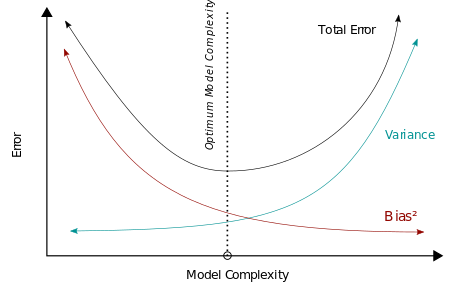
\includegraphics[width=0.7\textwidth]{Images/tradeoff_bias_variance.png}
    \caption{Bias-Complexiry tradeoff. A model with low complexity will have a low variance but an high bias. A model with high complexity will have a low bias but an high variance.}
    \label{fig:tradeoff_bias_accuracy}
\end{figure}
From now, we will assume that the inputs are in some space $\XX$ and the labels form a set $\mathcal{Y}:=\{1,\dots,K\}$. To learn an adequate classification model, we denote $\{(x_1,y_1),\dots,(x_\numsamples,y_\numsamples)\}$ the $\numsamples$ elements of $\XX\times\YY$ forming the training set. We furthermore assume that these inputs are independent and identically distributed (i.i.d.) from some distribution $\PP$ on $\XX\times\YY$. The aim is now to learn a function/hypothesis from these samples $h:\XX\to\YY$ to classify an input $x$ with a label $y$. To assess the quality of a classifier, the metric of interest is often the misclassification rate of the model, or the $0/1$ loss risk, and it is defined as:
\begin{align*}
\risk_{0/1}(h):=\PP(h(x)\neq y) = \EE_{(x,y)\sim\PP}\left[\mathbf{1}_{h(x)\neq y}\right]
\end{align*}
The optimal classifier, minimizing the standard risk is called the Bayes optimal classifier and is defined as $h(x) = \argmaxB_k\PP(y=k\mid x)$.
As the sampling distribution $\PP$ is usually unknown, the optimal Bayes classifier is also unknown. The accuracy is often empirically evaluated on a test set $\{(x'_1,y'_1),\dots,(x'_M,y'_M)\}$ independent from the training set and i.i.d. sampled from $\PP$.  To find this classifier $h$, we learn a function $\mathbf{f}:\XX\to\mathbb{R}^K$ returning scores, or logits, $(f_1(x),\dots,f_K(x))$ corresponding to each label. Then $h$ is set to $h(x)=\argmaxB_k f_k(x)$. The function $\mathbf{f}$ is usually learned by minimizing the empirical risk for a certain convenient loss function $\loss$ over some class of functions $\mathcal{H}$.
\begin{align*}
\inf_{\mathbf{f}\in\mathcal{H}}\riskemp_{\numsamples}(\mathbf{f}):= \frac{1}{\numsamples}\sum_{i=1}^\numsamples \loss(\mathbf{f}(x_i),y_i).
\end{align*}

This problem is called Empirical Risk Minimization (ERM). The theory of this problem has been widely studied and is well understood. It is often argued that there is a tradeoff on the ``size'' of $\mathcal{H}$: having a too small $\mathcal{H}$ may lead to underfitting, i.e. not enough parameters to describe the optimal possible function while a too large $\mathcal{H}$ may lead to overfitting, i.e. fitting too much training data. We often talk about bias-complexity tradeoff (see Figure~\ref{fig:tradeoff_bias_accuracy}). A penalty term $\Omega_{\mathcal{H}}(\mathbf{f})$ can also be added to the ERM objective to prevent from overfitting. This tradeoff was recently questioned by the double descent~\citep{belkin2019reconciling} phenomenon where overparametrized (i.e. number of parameters largely over the number of training samples) regimes lower the risk.

The presence of adversaries in classification questions the knowledge we have in standard statistical learning. Indeed most standard results do not hold in presence of adversaries, hence, opening a new research area dedicated to studying and understanding the classification problem in presence of adversarial attacks, and more importantly, deepens our understanding of  machine learning/deep learning in high dimensional regimes.




\subsection{Classification in Presence of Adversarial Attacks}

Though a model can be very well performing on natural samples, small perturbations of these natural samples can lead to unexpected and critical behaviours of classification models~\citep{biggio2013evasion,Szegedy2013IntriguingPO}. To formalize that, we will assume the existence of a ``perception'' distance $d:\XX^2\to\mathbb{R}$ such that a perturbation $x'$ of an input $x$ remains imperceptible if $d(x,x')\leq \varepsilon$ for some constant $\varepsilon\geq0$. This ``perception'' distance is difficult to define in practice. For images, the $\lVert\cdot\rVert_\infty$ distance over pixels is often used, but is not able to capture all imperceptible perturbations.  This choice is purely arbitrary: for instance, we will highlight in the manuscript that $\lVert\cdot\rVert_2$ perturbations can also be imperceptible while having a large $\lVert\cdot\rVert_\infty$. Image classification algorithms are also vulnerable to geometric perturbations, i.e. rotations and translations~\citep{kanbak2018geometric,engstrom2019exploring}. A typical example of an adversarial attack is shown in Figure~\ref{fig:adv-example}.


\begin{figure}
    \centering
    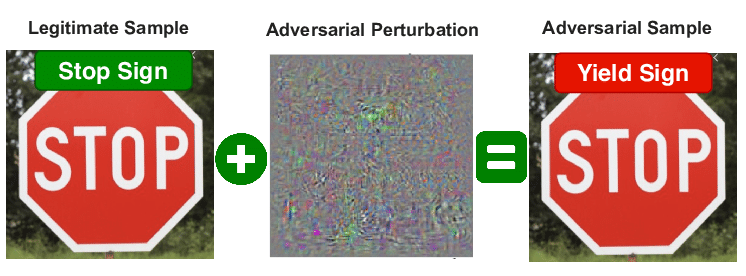
\includegraphics[width=0.9\textwidth]{Images/adv_image.png}
    \caption{Example of a pixel-level adversarial attack on a Stop Sign. It underlines the safety issues triggered by the possibility of such attacks.}
    \label{fig:adv-example}
\end{figure}

Therefore, the goal of an attacker is to craft an adversarial input $x'$ from an input $x$ that is imperceptible , i.e. $d(x,x')\leq \varepsilon$ and misclassifies the input, i.e. $h(x')\neq y$. Such a sample $x'$ is called an adversarial attack. The used criterion cannot be the misclassification rate anymore, we need to take into account the possible presence of an adversary that maliciously perturbs the input. We then define the robust/adversarial misclassification rate or robust/adversarial $0/1$ loss risk: 
\begin{align*}
\risk_{0/1}^{\varepsilon}(h)&:=\PP_{(x,y)}(\exists x'\in\XX\text{ s.t. } d(x,x')\leq \varepsilon \text{ and } h(x')\neq y)\\
&= \EE_{(x,y)\sim\PP}\left[\sup_{x'\in\XX\text{ s.t. } d(x,x')\leq \varepsilon}\mathbf{1}_{h(x')\neq y}\right]
\end{align*}
Akin standard risk minimization, we aim to learn a function $\mathbf{f}:\mathcal{X}\to\mathbb{R}^K$ such that $h(x)=\argmaxB_k f_k(x)$. Usually in adversarial classification we aim at solving the following optimization problem, that we will call adversarial empirical risk minimization:
\begin{align*}
\inf_{\mathbf{f}\in\mathcal{H}}\riskemp^\varepsilon_{\numsamples}(\mathbf{f}):= \frac{1}{\numsamples}\sum_{i=1}^\numsamples\sup_{x'\in\XX\text{ s.t. } d(x,x')\leq \varepsilon} \loss(\mathbf{f}(x_i),y_i).
\end{align*}
This problem is more challenging to tackle than the standard risk minimization  since it involves a hard inner supremum problem~\citep{madry2018towards}. Guarantees in the adversarial setting are therefore difficult to obtain both in terms of convergence and statistical guarantees. The usual technique to solve this problem is called Adversarial Training~\citep{goodfellow2014explaining,madry2018towards}. It consists in alternating inner and outer optimization problems. Such a technique improves in practice adversarial robustness but lacks theoretical guarantees. So far, most results and advances in understanding and harnessing adversarial attacks are empirical~\citep{ilyas2019adversarial,rice2020overfitting}, leaving many theoretical and practical questions open.  Moreover, robust models suffer from a performance drop and vulnerablity of models is currently still very high (see Table~\ref{table:sota-cifar}), which leaves room for substantial improvements.

\begin{table}[ht]
    \centering
    \begin{tabular}{c|c|c|c}
       \textbf{Attacker}  &  \textbf{Paper reference} & \textbf{Standard Acc.} & \textbf{Robust Acc.}  \\ \hline
        None & \citep{ZagoruykoK16} & 94.78\% & 0\%\\
        $\ell_\infty (\varepsilon=8/255)$&  \citep{rebuffi2021fixing}& 89.48\% & 62.76\%\\
        $\ell_2 (\varepsilon=0.5)$&  \citep{rebuffi2021fixing}& 91.79\% & 78.80\%\\
    \end{tabular}
    \caption{State of the art accuracies on adversarial tasks on a WideResNet 28x10~\citep{ZagoruykoK16}. Results are reported from~\citep{croce2020robustbench}}
\label{table:sota-cifar}
\end{table}

\section{Outline and Contributions}
We will first introduce in Chapter~\ref{chap:background} the necessary  background regarding Machine Learning and Adversarial Examples. We will then analyze  adversarial attacks from three complementary points of view outlined as follows.
\subsection{A Game Theoretic Approach to Adversarial Attacks}

A line of research, following~\cite{pinot2020randomization}, to understand adversarial classification is to rely on game theory. In Chapter~\ref{chap:game},  we will build on this approach and define precisely the motivations for both the attacker and the classifier. We will cast it naturally as a zero sum game. We will in particular, study the problem  of the existence of equilibria. More precisely, we will answer the following open question.
\medskip
\begin{tcolorbox}[colback=grund,colframe=rahmen,title=Question 1]
\textbf{What is the nature of equilibria in the adversarial examples game?}
\end{tcolorbox}
\medskip

In game theory, there are many types of equilibria. In this manuscript, we will focus on Stackelberg and Nash equilibria. We will show the existence of both when both the classifier and the attacker play randomized strategies. To reach such equilibria, the classifier will be random, and the attacker will move randomly the samples at a maximum distance of $\varepsilon$. Then, we will propose two different algorithms to compute the optimal randomized classifier in the case of a finite number of possible classifiers. We will finally propose a heuristic algorithm to train a mixture of neural networks and show experimentally the improvements we achieve over standard methods. This work was published at ICML2021~\citep{pmlr-v139-meunier21a}.




\subsection{Loss Consistency in Classification in Presence of an Adversary}
In standard classification, consistency with regards to $0/1$ loss is a desired property for the surrogate loss $\loss$ used to train the model. In short, a loss $\loss$ is said to be consistent if for every probability distribution, a sequence of classifiers $(f_n)$ that minimizes the risk associated with the loss $\loss$, it also minimizes the $0/1$ loss risk. Usually, in standard classification, the problem is simplified thanks to the notion of calibration. We will see that the question of consistency in the adversarial case is much harder. 
\medskip
\begin{tcolorbox}[colback=grund,colframe=rahmen,title=Question 2]
\textbf{Which losses are consistent with regards to the $0/1$ loss in the adversarial classification setting?}
\end{tcolorbox}
\medskip
We tackle this question by showing that usual convex losses are not calibrated for the adversarial classification loss. Hence this negative result emphasizes the difficulty of understanding the adversarial attack problem, and building provable defense mechanisms. We pave a way towards solving this question by proposing candidate losses and giving arguments for their consistency. This work has not been submitted for peer-reviewing yet. 
\subsection{Building Certifiable Models}

The last problem we deal with in this manuscript is the implementation of robust certifiable models. In short, a classifier is said to be certifiable at an input $x$ at level $\varepsilon$ if one can ensure there exist no adversarial examples in the ball of radius $\varepsilon$. This problem is challenging since it is far from trivial to come up with non vacuous bounds that are exploitable in practice.
\medskip
\begin{tcolorbox}[colback=grund,colframe=rahmen,title=Question 3]
\textbf{How to efficiently implement certifiable models with non-vacuous guarantees?}
\end{tcolorbox}
\medskip
To this end, we propose  a general method that enforces Lipschitzness on the predictions of neural networks. This method draws its inspiration from the continuous flow interpretation of residual networks. We provide discretization strategies and recover many existing methods to build $1$-Lipschitz layers in neural networks. In particular, we show that using a gradient flow of a convex function, our network is $1$-Lipschitz. Based on this insight, we design a Lipschitz layer, that we call Convex Potential Layer (CPL). We showing empirically and theoretically the robustness benefits of this approach. This work is under review and its preprint is available~\citep{meunier2021scalable}

% \section{Other Works in Appendix}
\subsection{Additional Works}
Additionally to the works we present in the main document, we also present some other contributions we made during the thesis. These are deferred to the appendices. 

Regarding adversarial examples, we will present additional works complete the study we lead in the main document:
\begin{itemize}
    \item \textbf{On the robustness of randomized classifiers to adversarial examples
    (see Appendix~\ref{paper:rando}):} we show that by adding a noise on an input of a classifier, we are able to get guarantees on the decision up to some level $\varepsilon$. This work was published at NeurIPS2019~\citep{pinot2019theoretical} and under review in an extended journal version~\citep{pinot2021robustness}.
    \item \textbf{Yet another but more efficient black-box adversarial attack: tiling and evolution strategies (see Appendix~\ref{paper:dfo-attacks}):} we provide a method based on evolutionary strategies to craft black-box adversarial attacks. This work is a preprint and has not been published~\citep{meunier2019yet}.
    \item \textbf{Advocating for Multiple Defense Strategies against Adversarial Examples    (see Appendix~\ref{paper:ecml_rat}):} We show that, in high-dimensional settings, the balls overlaps for two different $\ell^p$ norms are fundammentally different. This induces to rethink robustness against attacks using different norms. This work was published at a workshop at ECML2020~\citep{araujo2020advocating}.
    \item \textbf{Adversarial Attacks on Linear Contextual Bandits (see Appendix~\ref{paper:banditsattacks}):} we build provable attacks against online recommendation systems, namely Linear Contextual Bandits. This work was published at NeurIPS2020~\citep{garcelon2020adversarial}.
    \item \textbf{ROPUST: Improving Robustness through Fine-tuning with Photonic Processors and Synthetic Gradients (see Appendix~\ref{paper:ropust}):} we use an Optical Processor Unit (OPU) over existing SOTA defenses to improve adversarial robustness. This work was published at ICASSP2022~\citep{cappelli2021ropust}.
\end{itemize}
We  published a paper in optimal transport on \textbf{Equitable and Optimal Transport with Multiple Agents (see Appendix~\ref{paper:eot})} at AISTATS 2021~\citep{scetbon2021equitable} where we introduce a way to deal with multiple costs in optimal transport by equitably partitioning transport among costs. We also a published a paper at xxx on Conditional Indepedence Testing~\citep{scetbon2021ell} on \textbf{ an $\ell^p$-based Kernel Conditional Independence Test (see Appendix~\ref{paper:kerneltest})}. In this paper we present a new kernel-based Conditional Indepedence Test. Its advantages are its computational simplicity and a very simple asymptotic distribution under null hypothesis. Moreover, it performs competitively with other test for Conditional Independence.

With Olivier Teytaud, research scientist at Meta AI and co-supervisor of this thesis, we also published some works in the field of evolutionary algorithms:
\begin{itemize}

    \item \textbf{Variance Reduction for Better Sampling in Continuous Domains (see Appendix~\ref{paper:ppsn-rescaling})}: we show that, in one shot optimization, the optimal search distribution, used for the sampling, might be more peaked around the center of the distribution than the prior distribution modelling our uncertainty about the location of the optimum. This work was published at PPSN2020~\citep{ppsnrescaling}.
    \item \textbf{On averaging the best samples in evolutionary computation (see Appendix~\ref{paper:ppsn-kbest}):}  we prove mathematically that a single parent leads to a sub-optimal simple regret in the case of the sphere function. We provide a theoretically-based selection rate that leads to better progress rates. This work was published at PPSN2020~\citep*{ppsnkbest}.
    \item \textbf{Asymptotic convergence rates for averaging strategies (see Appendix~\ref{paper:foga}):} we extend the results from the previous paper to a wide class of functions including $C^3$ functions with unique optima. This work was published at FOGA2021~\citep{meunier2021asymptotic}.
    \item  \textbf{Black-Box Optimization Revisited: Improving Algorithm Selection Wizards through Massive Benchmarking (see Appendix~\ref{paper:benchmark}):} We propose a wide range of benchmarks integrated in Nevergrad~\citep{nevergrad} platform. This work was published in the journal TEVC~\citep{meunier2021black}.
    
\end{itemize}
% In addition to these works, we also add interest in adversarial attacks against online recommendation systems, namely Linear Contextual Bandits. We designed algorithms that provably fool in 

% We also published works in the field of Derivative Free Optimization FOLLOW
\chapter{Background}
\minitoc
\section{Classification}
First, we formalize the classification task:
\begin{itemize}
    \item Consider an input space $\mathcal{X}$, typically images. We assume this space is endowed an arbitrary metric $d$ possibly the perception distance or any $\ell_p$ norm. In the remaining of the manuscript, unless it is specified, $(\mathcal{X},d)$ will be a \textit{proper} (i.e. closed balls are compact) \textit{Polish} (i.e. completely separable) metric space. Note that for any norm $\lVert\cdot\rVert$,  $(\mathbb{R}^d,\lVert\cdot\rVert)$ is a proper Polish metric space.
    \item Each image $x\in \mathcal{X}$ has to be classified to a label $y$. We describe the set of labels $\mathcal{Y}:=\{1,\dots,K\}$ as descriptors of an input. For instance the label of an image will be the description of it. $\mathcal{Y}$ will be endowed with the trivial metric  $d'(y,y') = \mathbf{1}_{y\neq y'}$. Note that $(\mathcal{X}\times\mathcal{Y},d\oplus d')$ is a proper Polish space.
\end{itemize}
With such spaces, the space $(\mathcal{X}\times\mathcal{Y},d\oplus d')$ is also a proper Polish space. As in every classification problem, the data is sampled from probability distribution $\PP$. We will assume from now that the distribution we consider are Borel. For any Polish Space $\mathcal{Z}$, we will denot $\mathcal{B}(\mathcal{Z})$ the Borel $\sigma$-algebra and the set of Borel distributions $\mathcal{Z}$ over will be denoted $\mathcal{M}_+^1(\mathcal{Z})$. We also recall the notion of \textit{universal measurability}: a set $A\subset \mathcal{Z}$ is said to be universally measurable if it measurable for every \textit{complete} Borel probability measures.

In standard classification, we aim at learning a (universally or Borel) measurable function $h:\mathcal{X}\to\mathcal{Y}$ minimizing the $0/1$ loss risk:
\begin{align}
   \risk_{0/1}(h):=\PP(h(x)\neq y) = \EE_{(x,y)\sim\PP}\left[\mathbf{1}_{h(x)\neq y}\right]
\end{align}
Note that this quantity is well defined when $h$ is measurable. The optimal classifier is called the Bayes Optimal classifier and is defined as $h(x) = \argmaxB_k\PP(y=k\mid x)$. One can note, using disintegration theorem that $h$ is indeed Borel measurable.

However in practice, the access to the Bayes Optimal classifier is impossible because it requires full knowledge on the probability distribution $\PP$ which is not the case in general. Let assume having access to a training set of $n$ data points $\{(x_1,y_1),\dots,(x_n,y_n)\}$. The knowledge of the Bayes classifier on training points would not be sufficient to have generalization properties for the classifier on out-of-sample data points because such functions would overfit the training set. Hence one need to reduce the search space of measurable functions to a much smaller one, we will denote $\mathcal{H}$. More precisely, for binary classification (i.e $\mathcal{Y}:=\{-1,+1\})$, we aim at learning a function $\mathbf{f}:\XX\to\mathbb{R}$ such that $h(x)=\sign(f(x))$ (with a convention on $sign(0)$). In multilabel classification (i.e $|\mathcal{Y}|\geq2$), we learn a function $\mathbf{f}:\XX\to\mathbb{R}^K$ and $h$ is set to $h(x)=\argmaxB_k f_k(x)$. Minimizing directly the $0/1$ loss risk is a NP-hard problem in general CITE. Then one needs to minimize a well-chosen loss function $L$. A \textit{loss function} $L:\mathbb{R}^K\times\mathcal{Y}\to\mathbb{R}$ will be without loss of generality a non negative Borel measurable function. An example of such a loss is the cross entropy loss defined as:
\begin{align*}
    L(\mathbf{f}(x),y)=\sum_{i=1}^n
\end{align*}

The study of which loss is suited for classification has been a widely studied topic. Hence the learning objective is then defined as:

\begin{align*}
\inf_{\mathbf{f}\in\mathcal{H}}\riskemp_{n}(\mathbf{f}):= \frac{1}{n}\sum_{i=1}^nL(\mathbf{f}(x_i),y_i).
\end{align*}

define 


% Instead, we aim at learning either a classifier $h\in\mathcal{H}$ such that:



\section{Background in adversarial classification}
Adversarial classification, we aim at learning a a (universally or Borel) measurable function $h:\mathcal{X}\to\mathcal{Y}$ minimizing the $0/1$ loss risk: 
\begin{align*}
\risk^\varepsilon_{0/1}(h)&:=\PP_{(x,y)}(\exists x'\in\XX\text{ s.t. } d(x,x')\leq \varepsilon \text{ and } h(x')\neq y)\\
&= \EE_{(x,y)\sim\PP}\left[\sup_{x'\in\XX\text{ s.t. } d(x,x')\leq \varepsilon}\mathbf{1}_{h(x')\neq y}\right]
\end{align*}
The definition of this quantity is not immediate and requires a proposition.

\begin{prop}
For any $h$ Borel measurable, the adversarial risk is well defined $\risk^\varepsilon_{0/1}(h)$.
\end{prop}

The existence of a minimizer for adversarial risk is a difficult question, that was partially answered in CITE, which states, under some mild conditions, that the minimum is attained over the set of universally measurable functions.


 define general adversarial loss.



The question of the loss function 


\subsection{Standard datasets in Classification}
Images are embedding in pixels laying in $[0,255]$ and then normalized to $[0,1]$. These images can be black and white, hence encoded on only one channel, or colorful and then encoded on three channels, often, Red, Green, Blue (RGB). The images are of diverse qualities, the number of pixels quantifies this quality.  In image classification evaluation, three datasets are mainly used:
\begin{itemize}
    \item \textbf{MNIST~\citep{lecun1998mnist}:} A dataset of black and white low-quality images representing the $10$ digits. The training set contains $50000$ images and test set $10000$ images. These images are of dimension $28\times28\times 1$ ($784$ in total). This dataset is known to be easy ($>99\%$ can be obtained using simple classifiers). In adversarial classification, the problem is also easy to be solved. Evaluation MNIST is not sufficient to assess the performance of a classifier or even a defense against adversarial examples.
    \item \textbf{CIFAR10 and CIFAR100~\citep{krizhevsky2009learning}:} Datasets of colored low-quality images representing the $10$ labels and $100$ labels for respectively CIFAR10 and CIFAR100. Each training set contains $50000$ images and test set $10000$ images. These images are of dimension $32\times32\times 1$ ($3072$ in total). The current state-of-the-art on CIFAR10 in standard classification is $>99\%$ of accuracy, but asks advanced methods to reach such a score. On CIFAR100, the current state-of-the-art is around $94\%$. In adversarial classification both datasets are challenging and difficult. The evolution of state-of-the-art in adversarial classification is available in RobustBench\footnote{\url{https://robustbench.github.io/}}. Benchmark in adversarial classification are often made on these datasets.
    \item \textbf{ImageNet~\citep{imagenet_cvpr09}:} ImageNet refers to a dataset containing $1.2$ million of images labeled into $1000$ classes. Images are of diverse qualities, but often $224\times224\times 3$ (dimension $150528$ in total). The current state-of-the-art on ImageNet is about $87\%$. There is no need to say that adversarial classification on ImageNet is still a very-challenging task. Further than the standard dataset, ImageNet project is still in development: the project gathers $14197122$ images and $21841$ labels on August 31th, 2021.   


\end{itemize}
\section{Background on adversarial examples}
\subsection{Crafting adversarial examples}

What is the more striking about adversarial examples is the facility to craft them. Let consider an attacker that aim  finding an adversarial perturbation $x'$ of an input $x$ for a given classifier $\mathbf{f}$.  Given a differentiable loss $L$, typically the cross-entropy, the attacker usually maximize the following objective:

\begin{align}
    \max_{x'\in\XX\text{ s.t. } d(x,x')\leq \varepsilon}L\left(\mathbf{f}(x'), y)\right).
\end{align}
To do so, many attacks were proposed that we will categorize in two parts: 
\begin{itemize}
    \item \textbf{White box attacks:} the attacker have the full knowledge of the function $\mathbf{f}$ and its parameters. Hence this attacks are often based on the gradient of the former objective. The most popular white box attacks are CITE
    \item \textbf{Black box attacks:} the attacker have no knowledge on the classifier parameters. The attacker have limited access to the classifier, e.g. he can only access logits or predicted class for instance.
    
\end{itemize}

\subsection{Which Perception Distance to Use?}

The choice of the 
% \section{Optimal Transportation}

% As seen Optimal Transportation seems to play a central role in understanding adversarial attacks, 
% For any Polish space $\mathcal{Z}$, we denote $\mathcal{M}_+^1(\mathcal{Z})$ the Polish space of Borel probability measures on $\mathcal{Z}$. Let us assume the data is drawn from $\PP\in\mathcal{M}_+^1(\mathcal{X}\times\mathcal{Y})$. Let $(\Theta,d_\Theta)$ be a Polish space (not necessarily proper) representing the set of classifier parameters (for instance neural networks). We also define a loss function: $l:\Theta\times (\mathcal{X}\times\mathcal{Y})\to [0,\infty)$ satisfying the following set of assumptions.
\chapter{Related Work}
\label{chap:rw}
\minitoc
\section{Q1}

\subsection{Optimal Transport}
Optimal Transport have gained interest in Machine Learning applications during the past years. Indeed, Optimal Transport has the ability to model many problems as Generative Adversarial Networks~\citep{arjovsky2017wasserstein}, or in Robust Learning~\citep{xxx}. The computation methods for optimal transport problems have also been considerably improved recently.  We recall the main concepts from the Optimal Transport Theory. Originally introduced by Monge, this Optimal Transport was a problem where the aim was to move some quantity $x$ to some places $y$ while minimizing the total cost of transport. Formally, the problem was c



\begin{definition}[Couplings between distributions] 
    Let $\ZZ$ be a Polish space. Let $\PP$ and $\QQ$ be two Borel probability distributions over $\ZZ$. The set of coupling distributions between $\PP$ and $\QQ$ is defined as:
    \begin{align*}
        \Gamma_{\PP,\QQ}:=\left\{\gamma\in\mathcal{M}^1_+(\ZZ^2)\mid~ \Pi_{1,\sharp}\gamma = \PP,~\Pi_{2,\sharp}\gamma = \QQ\right\}
    \end{align*}
where $\Pi_{i,\sharp}$ represents the push-forward of the projection on the $i$-th component.
\end{definition}
\begin{definition}[Optimal Transport]
Let $\ZZ$ be a Polish space. Let $c:\ZZ\to\bar{\RR}_+$ be a lower semi-continuous non-negative function. Let $\PP$ and $\QQ$ be two  Borel probability distributions over $\ZZ$. The Optimal Transport problem or Wasserstein problem between $\PP$ and $\QQ$ associated with cost function $c$ is defined as:
\begin{align*}
    W_c(\PP,\QQ):=\inf_{\gamma\in\Gamma_{\PP,\QQ}}\int c(x,y) d\gamma(x,y) = \inf_{\gamma\in\Gamma_{\PP,\QQ}}\mathbb{E}_{(x,y)\sim\gamma}\left[c(x,y) \right]
\end{align*} 
\end{definition}
The infimum is attained.
When $\XX$ is endowed with ground metric $d$, one can endow the space of probability distributions with bounded $p$-moments with a metric named the Wasserstein-$p$ metric defined as:
\begin{align*}
    D_p(\PP,\QQ):=\inf_{\gamma\in\Gamma_{\PP,\QQ}}\mathbb{E}_{(x,y)\sim\gamma}\left[d^p(x,y) \right]^{1/p}
\end{align*}
With this metric, the space of probability distributions with bounded $p$-moments metrizes the weak topology of measures. When $p=\infty$, the $D_\infty$ be be defined in the limit as:
\begin{align*}
    D_\infty(\PP,\QQ):=\inf_{\gamma\in\Gamma_{\PP,\QQ}}\gamma-\esssup_{(x,y)} d(x,y) 
\end{align*}
\paragraph{Kantorovich Duality.} A fundammental theorem in Optimal Transportation is the Kantorovich duality theorem as follows:

\begin{thm}[Kantorovich duality]
    Let $\ZZ$ be a Polish space. Let $c:\ZZ\to\bar{\RR}_+$ be a lower semi-continuous non-negative function. Let $\PP$ and $\QQ$ be two Borel probability distributions over $\ZZ$. Then   the following strong duality theorem holds:
\begin{align*}
    W_c(\PP,\QQ)=\sup_{f,g\in C(\ZZ),~f\oplus g\leq c}   \int fd\PP+\int fd\QQ
\end{align*}
where for all $x,y\in\ZZ$, $f\oplus g(x,y):=f(x)+g(y)$. 
\end{thm}
One can find a proof of this result in~\citep{villani2003topics}. The main arguments are that the dual of continuous functions on  a compact space is the space of Radon measures, and the Rockafellar duality theorem. 

\paragraph{Adversarial Risk Minimization as an Optimal Transport Pronlem.} Let $\PP$ be a distribution over the input-label space $\XX\times\YY$. We recall that the problem of adversarial risk minimization is defined as
\begin{align*}
    \risk_{\varepsilon,\PP}^\star = \inf_{h} \PP_{(x,y)}\left[\exists x'\in B_\varepsilon(x),~h(x')\neq y\right]
\end{align*}
A recent line of work draw important links between   $\risk_{\varepsilon,\PP}^\star$ and Optimal Transport problems in the case of binary classification ($\YY=\{-1,+1\}$) the space $\XX$ satisfy a midpoint property, i.e. TODO. It was shown that in this case:
\begin{align*}
\risk_{\varepsilon,\PP}^\star = \frac12-\frac12 W_{c_\varepsilon}(\PP,\PP^S)
\end{align*}
where $\PP^S := T^S_\sharp \PP$ with $T^S(x,y) = (x,-y)$ and
\begin{align*}
    c_\varepsilon\left((x,y),(x',y')\right) = xxx
\end{align*}

Note that $T^S$ only switches the label of pair $(x,y)$. When $\varepsilon=0$, $W_{c_\varepsilon}(\PP,\PP^S)$ equals the total variation distance between $\PP$ and $\PP^S$, which was a result proved in~\citep{xxx}.
While this property does not have practical properties yet, there is a hope that this relation might help at building more robust classifiers to adversarial examples. 

\subsection{Distributionally Robust Optimization}

In this section, we give an introduction to distributionally robust optimization problems. We see these problems are related to adversarial attacks problems. We draw links in this introduction.  Let $\ZZ$ and $\Theta$ be Polish spaces. Let $\PP$ be a Borel probability distribution over $\ZZ$. Let $f:\Theta\times\ZZ\to\RR$ be an upper semi continuous function in its second variable. Let us consider the following problem:
\begin{align}
    \label{eq:min-objective}
    \min_{\theta\in\Theta} \mathbb{E}_{z\sim\PP}\left[f(z)\right] = \min_{\theta\in\Theta} \int f(\theta,z)d\PP(z)
\end{align}
This problem can typically be a risk minimization problem in Machine Learning when $\PP$ is a distribution over input-label pairs and $\Theta$ is a parameter space for the classifier. A distributionally robust optimization (DRO) problem is a problem similar to Equation~\eqref{eq:min-objective}, but the learner aims at being robust to a change in the distribution $\PP$. Typically if $D$ is an uncertainty metric for distribubtions. Formally, the DRO problem is casted as follows:
\begin{align*}
    \min_{\theta\in\Theta}\sup_{\QQ\in\mathcal{M}^1_+(\ZZ)\mid~D(\PP,\QQ)\leq \varepsilon}\mathbb{E}_{z\sim\QQ}\left[f(z)\right]
\end{align*}
For instance, $D$ be a Kullback-Leibler etc CITE

In the case of Wasserstein uncertainty sets, let $c:\ZZ\to\bar{\RR}_+$ be a lower semi-continuous non-negative function. Then a  Wasserstein distributionally robust optimization (DRO) problem is defined as follows:
\begin{align*}
    \min_{\theta\in\Theta}\sup_{\QQ\in\mathcal{M}^1_+(\ZZ)\mid~W_c(\PP,\QQ)\leq \varepsilon}\mathbb{E}_{z\sim\QQ}\left[f(z)\right]
\end{align*}

Then we can define the Wasserstein balls as 
\begin{align*}
    \mathcal{B}_{c}(\PP,\varepsilon) := \left\{\QQ\in \mathcal{M}^+_1(\mathcal{Z})\mid W_c(\PP,\QQ)\leq \varepsilon\right\}
\end{align*}
This problem induces an attack on the distribution $\PP$. Informally, one can interpret a Wassertein ball as an attacker moving each point $x$ of the distribution $\PP$ to a distribution $\QQ_x$ so that the average ``distance'' $\mathbb{E}_{x\sim\PP}\left[\mathbb{E}_{y\sim\QQ_x}\left[c(x,y)\right]\right]$ at most equal to $\varepsilon$. With this interpretation, we can start linking the Wasserstein DRO problem to the adversarial learning problem. Indeed in the adversarial attack problem, the attacker is authorized to move each point to another at distance at most $\varepsilon$, i.e. he is authorized a mapping $T$ such that $d(x,T(x))\leq \varepsilon$ for every $x$ almost surely. 
\paragraph{Properties of Wasserstein balls.} The Wasserstein balls inherits from nice properties. Since $\QQ\mapsto  W_c(\PP,\QQ)$ is convex, they are convex sets. Moreover the function $\QQ\mapsto  W_c(\PP,\QQ)$ is lower semi-continuous for the narrow topology of measures, then the set $\mathcal{B}_{c}(\PP,\eta) $ is closed for the narrow topology too. Concerning the compactness of this set, if $\ZZ$ is compact then the set $\mathcal{B}_{c}(\PP,\eta) $ is also compact as a closed subset of the compact set $\mathcal{M}^+_1(\mathcal{Z})$.~\cite{yue2020linear} proved the compactness for $l^p$ distances. In general, compactness is a case by case question. 


\paragraph{Duality results} The problem of computing DRO solutions is difficult become it concerns optimization over distribution. A strong duality leading to a relaxation of the problem was proved by~\cite{blanchet2019quantifying}. We state this theorem as follows.


\begin{thm}[Wasserstein DRO duality]
    Let $\PP$ be a Borel probability distribution over $\ZZ$. Let $f:\ZZ\to\RR$ be an upper semi continuous function. Let $c:\ZZ\to\RR_+$ be a lower semi-continuous non-negative function. 
    \begin{align*}
        \sup_{\QQ\in\mathcal{M}^1_+(\ZZ)\mid~W_c(\PP,\QQ)\leq \varepsilon}\mathbb{E}_{z\sim\QQ}\left[f(z)\right] = \inf_{\lambda\geq 0}\mathbb{E}_{z\sim\PP}\left[\sup_{z'\in\ZZ}f(z')-\lambda c(z,z')\right] +\lambda\varepsilon
    \end{align*}
  
\end{thm}

This theorem was proved by~\citep{blanchet2019quantifying} using similar arguments to Kantorovich duality. The link with the adversarial attack problem is made clearer with this theorem. Indeed $\mathbb{E}_{z\sim\PP}\left[\sup_{z'\in\ZZ}f(z')-\lambda c(z,z')\right]$ is closed to the adversarial attacks problem. We will make a direct link in the Chapter~\ref{chap:game}.


\paragraph{Adversarial classification as a Wasserstein-$\infty$ DRO problem.} It has been shown recently that the Adversarial classification problem could be casted as a Wasserstein-$\infty$ problem associated with a well-suited cost function. The previous result from~\citep{blanchet2019quantifying} does not directly apply to Wasserstein-$\infty$ distances but can be adapted. The Wasserstein-$\infty$ DRO problem can be understood as follows: each point $x$ of the distribution $\PP$ can be moved to a distribution $\QQ_x$ so that the worst-case ``distance'' $c(x,y)$ is smaller that $\varepsilon$. In general, one can prove the following result that proves that the adversarial classification problem is actually a Wasserstein-$\infty$ DRO problem.

\begin{thm}[Duality for Wasserstein-$\infty$ DRO]
Let $\ZZ$ be a Polish space. Let $\PP$ be a probability distribubtion over $\ZZ$. Let $c$ be a non-negative lower-semicontinuous function over $\ZZ^2$ and $f:\ZZ\to \RR$ be a Borel measurable function. Then the following strong duality holds
    \begin{align*}
        \sup_{\QQ|~W_{\infty,c}(\PP,\QQ)\leq \varepsilon}\mathbb{E}_{z\sim\QQ}\left[f(z)\right] = \mathbb{E}_{z\sim\PP}\left[\sup_{z'\in \ZZ|~c(z,z')\leq\varepsilon} f(z')\right]
    \end{align*}  
\end{thm}
This result can be found in special case in~\citep{xxx}. For sake of completeness, we provide a proof of the result. 
\begin{proof}
    TODO
\end{proof}

When the problem is a classification problem (i.e., $\ZZ=\XX\times\YY$ with $\YY = [K]$), one can replace $f$ with  $\loss(f(x),y)$ with $\loss$ a measurable loss function and set the cost $c$ equals to:
\begin{align*}
    c((x,y),(x',y')) := \left\{
        \begin{array}{ll}
            d(x,x') & \mbox{if } y = y'\\
            +\infty & \mbox{otherwise.}
        \end{array}
    \right.
\end{align*} 
Hence, we recover the Adversarial classification problem using a Wasserstein-$\infty$ DRO problem. We will see in Chapter~\ref{xxx}, the geometric and topological properties of this set. 


\subsection{Game Theory and Adversarial Learning}

A recent line of work focus on the game theory of adversarial examples. 
\section{Surrogate losses in the Adversarial Setting}
\label{sec:rw-q2}
To account for the possibility of an adversary manipulating the inputs at test time, we need to revisit the standard risk minimization problem by penalizing any classification model that might change its decision when the point of interest is slightly changed. Essentially, this is done by replacing the standard (pointwise) $0/1$ loss with an adversarial version that mimics its behavior locally but also penalizes any error in a given region around the point on which it is evaluated.


Yet, just like the $0/1$ loss, its adversarial counterpart is not convex, which renders the risk minimization difficult. To circumvent this limitation, we take inspiration from the standard learning theory approach which consists in solving a simpler optimization problem where the non-convex loss function is replaced by a convex surrogate. In general, the surrogate loss is chosen to have a property called \emph{consistency}~\citep{zhang2004statistical,bartlett2006convexity,steinwart2007compare}, which essentially guarantees that any sequence of classifiers that minimizes the surrogate objective must also be a sequence that minimizes the Bayes risk. In the context of standard classification, a large family of convex losses, called \textit{classifier-consistent}, exhibits this property. This class notoriously includes the hinge loss, the logistic loss and the square loss. 

However, the adversarial version of these surrogate losses needs not to have the same consistency properties with respect to the adversarial $0/1$ loss. In fact, most existing results in the standard framework rely on a reduction of the global consistency problem to a local point-wise problem, called \textit{calibration}. However, the same approach is not feasible in the adversarial setting, because the new losses are by nature non-point-wise. Then the optimum for a given input may depend on yet a whole other set of inputs~\citep{awasthi2021calibration,awasthi2021finer}. Studying the concepts of calibration and consistency in an adversarial context remains an open and understudied issue. 
%In fact, this is a rather complex area of research as the results can easily become meaningless or inaccurate when obtained without scrupulous and rigorous analysis. 
Furthermore, this is a complex and technical area of research, that requires a rigorous analysis, since small tweaks in definitions can quickly make results meaningless or inaccurate.
This difficulty is illustrated in the literature, where articles published in high profile conferences tend to contradict or refute each other~\cite{bao2020calibrated,awasthi2021calibration,awasthi2021finer}. 





%\subsection{Setting and Notations}

%\subsection{Setting and Notations}
\paragraph{Notations.} In this section, let us consider a classification task with input space $\mathcal{X}$ and output space $\mathcal{Y}=\{-1,+1\}$. Let $(\mathcal{X},d)$ be a proper Polish (i.e. completely separable) metric space representing the inputs space. For all $x\in\mathcal{X}$ and $\delta>0$, we denote $B_\delta(x)$ the closed ball of radius $\delta$ and center $x$. We also assume that for all $x\in\mathcal{X}$ and $\delta>0$,  $B_\delta(x)$ contains at least two points\footnote{For instance, for any norm $\lVert\cdot\rVert$,  $(\mathbb{R}^d,\lVert \cdot \rVert)$ is a Polish metric space satisfying this property.}. Let us also endow $\mathcal{Y}$ with the trivial metric  $d'(y,y') = \mathbf{1}_{y\neq y'}$. Then the space $(\mathcal{X}\times\mathcal{Y},d\oplus d')$ is a proper Polish space. For any Polish space $\mathcal{Z}$, we denote $\mathcal{M}_+^1(\mathcal{Z})$ the Polish space of Borel probability measures on $\mathcal{Z}$. We will denote $\mathcal{F}(\mathcal{Z})$ the space of real valued Borel measurable functions on $\mathcal{Z}$. Finally, we denote $\bar{\RR}:=\RR\cup\{\-\infty,+\infty\}$.


\subsection{Notions of Calibration and Consistency}

The $0/1$-loss is both non-continuous and non-convex, and its direct minimization is a difficult problem. The concepts of calibration and consistency aim at identifying the properties that a loss must satisfy in order to be a good surrogate for the minimization of the $0/1$-loss. In this section, we define these two concepts and explain the difference between them. First of all, we need to give a general definition of a loss function.

\begin{definition}[Loss function] A loss function is a function $L:\mathcal{X}\times\mathcal{Y}\times \mathcal{F}(\mathcal{X})\to \mathbb{R}$ such that $L(\cdot,\cdot,f)$ is a Borel measurable for all $f\in\mathcal{F}(\mathcal{X})$. 
\end{definition}
Note that this definition is not specific to the standard neither adversarial case. In general, a loss can either depend only on $f(x)$, or on other points related to $x$ (e.g. the set of points within a distance $\varepsilon$ of $x$). We now recall the definition of the risk associated with a loss $L$ and a distribution $\PP$. 
\begin{definition}[$L$-risk of a classifier]
For a given loss function $L$, and a Borel probability distribution $\PP$ over $\XX\times\YY$ we define the risk of a classifier $f$ associated with the loss $L$ and a distribution $\PP$ as
\begin{align*}
     \risk_{L,\PP}(f) := \mathbb{E}_{(x,y)\sim\PP}\left[L(x,y,f)\right].
\end{align*}
We also define the optimal risk associated with the loss $L$ as
\begin{align*}
         \risk_{L,\PP}^\star := \inf_{f\in\mathcal{F}(\XX)}\risk_{L,\PP}(f)\quad.
\end{align*}
\end{definition}

Essentially, the risk of a classifier is defined as the average loss over the distribution $\PP$. When the loss $L$ is difficult to optimize in practice (e.g when it is non-convex or non-differentiable),  it is often preferred to optimize a surrogate loss function instead. In the literature~\citep{zhang2004statistical,bartlett2006convexity,steinwart2007compare}, the notion of surrogate losses has been studied as a consistency problem. In a nutshell, a surrogate loss is said to be consistent if any minimizing sequence of classifiers for the risk associated with the surrogate loss is also one for the risk associated with $L$. Formally, the notion of consistency is as  follows.

\begin{definition}[Consistency]
Let $L_1$ and $L_2$ be two loss functions. For a given $\PP\in\mathcal{M}_1^+(\XX\times\YY)$, $L_2$ is said to be consistent for $\PP$ with respect to $L_1$ if for all sequences $(f_n)_n \in \mathcal{F}(\mathcal{X})^\mathbb{N}$ :
\begin{align}
    \risk_{L_2,\PP}(f_n)\to \risk_{L_2,\PP}^\star\implies\risk_{L_1,\PP}(f_n)\to \risk_{L_1,\PP}^\star
\end{align}
Furthermore, $L_2$ is said consistent with respect to a loss $L_1$ the above holds for any distribution $\PP$.
\end{definition}

\textcolor{black}{
Note that one can reformulate equivalently the previous definition as follows.  For all $\epsilon>0$, there exists $\delta>0$ such that for every $f\in\mathcal{F}(\XX)$,
\begin{align*}
    \risk_{L_2,\PP}(f)- \risk_{L_2,\PP}^\star\leq\delta\implies\risk_{L_1,\PP}(f)-\risk_{L_1,\PP}^\star\leq\epsilon
\end{align*}
}

Consistency is in general a difficult problem to study because of its high dependency on the distribution $\PP$ at hand. Accordingly, several previous works~\citep{zhang2004statistical,bartlett2002rademacher,steinwart2007compare} introduced a weaker notion to study consistency from pointwise viewpoint. The simplified notion is called \textit{calibration} and corresponds to consistency when $\PP$ is a combination of Dirac distributions. The main building block in the analysis of the calibration problem is the calibration function, defined as follows.

\begin{definition}[Calibration function]
Let $L$ be a loss function. The calibration function $\mathcal{C}_L$ is 
\begin{align*}
    \mathcal{C}_L(x,\eta,f):=\eta L(x,1,f) +(1-\eta) L(x,-1,f),
\end{align*}
for any $\eta\in[0,1]$, $x\in\mathcal{X}$ and $f\in\mathcal{F}(\mathcal{X})$. We also define the optimal calibration function as
\begin{align*}
        \mathcal{C}^\star_L(x,\eta):=\inf_{f\in\mathcal{\mathcal{F}(\mathcal{X})}}\mathcal{C}_L(x,\eta,f).
\end{align*}

\end{definition}

Note that for any $x\in\XX$ and $\eta\in[0,1]$, $\mathcal{C}_L(x,\eta,f) =\risk_{L,\PP}(f)$ with $\PP = \eta \delta_{(x,+1)}+ (1-\eta)\delta_{(x,-1)}$. The calibration function thus corresponds then to a pointwise notion of the risk, evaluated at point $x$. We now define what one means by calibration of a surrogate loss.

\begin{definition}[Calibration]
Let $L_1$ and $L_2$ be two loss functions. We say that $L_2$ is \emph{calibrated} with regards to $L_1$ if for every $\epsilon>0$, $\eta\in[0,1]$ and $x\in\mathcal{X}$, there exists $ \delta>0$ such that for all $f\in\mathcal{F}(\mathcal{X})$,
\begin{align*}
    \mathcal{C}_{L_2}(x,\eta,f)- &\mathcal{C}^\star_{L_2}(x,\eta)\leq\delta\implies\mathcal{C}_{L_1}(x,\eta,f)- \mathcal{C}^\star_{L_1}(x,\eta)\leq \epsilon.
\end{align*}

Furthermore, we say that $L_2$ is \emph{uniformly calibrated} with regards to $L_1$ if for every $\epsilon>0$, there exists $ \delta>0$ such that for all $\eta\in[0,1]$, $x\in\mathcal{X}$ and $f\in\mathcal{F}(\mathcal{X})$ we have
\begin{align*}
    \mathcal{C}_{L_2}(x,\eta,f)- \mathcal{C}^\star_{L_2}(x,\eta)\leq\delta\implies\mathcal{C}_{L_1}(x,\eta,f)- \mathcal{C}^\star_{L_1}(x,\eta)\leq \epsilon.
\end{align*}
\end{definition}

\textcolor{black}{
Similarly to consistency, one also give a sequential characterization for calibration and uniform calibration: $L_2$ is \emph{calibrated} with regards to $L_1$ if for all $\eta\in[0,1]$, $x\in\mathcal{X}$, for all $(f_n)_n\in\mathcal{F}(\XX)^\mathbb{N}$:
\begin{align*}
   \mathcal{C}_{L_2}(x,\eta,f)&- \mathcal{C}^\star_{L_2}(x,\eta)\xrightarrow[n\to\infty]{} 0
   \implies \mathcal{C}_{L_1}(x,\eta,f)- \mathcal{C}^\star_{L_1}(x,\eta)\xrightarrow[n\to\infty]{} 0\quad.
\end{align*}
} 
\textcolor{black}{
Also, $L_2$ is \emph{uniformly calibrated} with regards to $L_1$ if for all $(f_n)_n\in\mathcal{F}(\XX)^\mathbb{N}$:
\begin{align*}
    \sup_{\eta\in[0,1],x\in\mathcal{X}} &\mathcal{C}_{L_2}(x,\eta,f)- \mathcal{C}^\star_{L_2}(x,\eta)\xrightarrow[n\to\infty]{} 0\\\
    &\implies\sup_{\eta\in[0,1],x\in\mathcal{X}} \mathcal{C}_{L_1}(x,\eta,f)- \mathcal{C}^\star_{L_1}(x,\eta)\xrightarrow[n\to\infty]{} 0\quad.
\end{align*} }

%\textcolor{blue}{Raf: I would choose one of the characterization (sequential or not) and use it for both calibration and consictency.}

\textbf{Connection between calibration and consistency.}
It is always true that calibration is a necessary condition for consistency. Yet there is no reason, in general, for the converse to be true. However, in the specific context usually studied in the literature (i.e., the standard classification with a well-defined $0/1$-loss), the notions of consistency and calibration have been shown to be equivalent.~\citep{zhang2004statistical,bartlett2006convexity,steinwart2007compare}. In the next section, we come back on existing results regarding calibration and consistency in this specific (standard) classification setting. 


\subsection{Existing Results in the Standard Classification Setting}

Classification is a standard task in machine learning that consists in finding a classification function $h:\XX\to\YY$ that maps an input $x$ to a label $y$. In binary classification, $h$ is often defined as the sign of a real valued function $f \in \mathcal{F}(\XX)$. The loss usually used to characterize classification tasks corresponds to the accuracy of the classifier $h$. When $h$ is defined as above, this loss is defined as follows.




\begin{definition}[$0/1$ loss]
Let $f \in \mathcal{F}(\XX)$. We define the \emph{$0/1$ loss} as follows
\begin{align*}
     l_{0/1}(x,y,f)=\mathbf{1}_{y\times\text{sign}(f(x))\leq 0}
\end{align*}
 with a convention for the sign, e.g. $sign(0) = 1$.  We will denote $\risk_{\PP}(f) :=\risk_{l_{0/1},\PP}(f)$,  $\risk_{\PP}^\star :=\risk_{l_{0/1},\PP}^\star$, $\mathcal{C}(x,\eta,f):= \mathcal{C}_{l_{0/1}}(x,\eta,f)$ and $\mathcal{C}^\star(x,\eta):= \mathcal{C}^\star_{l_{0/1}}(x,\eta)$.
\end{definition}

Note that this $0/1$-loss is different from the one introduced by~\citet{bao2020calibrated,awasthi2021calibration,awasthi2021finer}: they used $\mathbf{1}_{y\times f(x)\leq 0}$ which is an usual $0/1$ loss but unadapted to consistency and calibrated study. This loss penalizes indecision: i.e. predicting $0$ would lead to a pointwise risk of $1$ for $y=1$ and $y=-1$ while the $0/1$ loss $l_{0/1}$ returns $1$ for $y=1$ and $0$ for $y=-1$. This definition was used by~\citet{bao2020calibrated,awasthi2021calibration,awasthi2021finer} to prove their calibration and consistency results. While~\citet{bartlett2006convexity} was not explicit on the choice for the $0/1$ loss,~\citet{steinwart2007compare} explicitly mentions that the $0/1$ loss is not a margin loss. The use of this loss is not suited for studying consistency and leads to inaccurate results as shown in the following counterexample. On $\mathcal{X}= \RR$, let $\PP$ defined as 
$\PP = \frac12\left(\delta_{x=0,y=1}+\delta_{x=0,y=-1}\right)$ and $\phi:\mathbb{R}\to\mathbb{R}$ be a margin based loss. The $\phi$-risk minimization problem writes $\inf_{\alpha} \frac{1}{2} (\phi(\alpha)+\phi(-\alpha))$. For any convex functional $\phi$ the optimum is attained for $\alpha=0$. $f_n:x\mapsto 0$ is a minimizing sequence for the $\phi$-risk. However $R_{l_{\leq}}(f_n)=1$ for all $n$ and $R_{l_{\leq}}^*=\frac{1}{2}$. Then we deduce that no convex margin based loss is consistent wrt $l_{\leq}$. Consequently, the $0/1$ loss to be used in adversarial consistency needs to be $l_{0/1,\varepsilon}(x,y,f) = \sup_{x'\in B_\varepsilon(x)} \mathbf{1}_{y\text{sign}(f(x))\leq 0}$, otherwise the obtained results might be innacurate.



Some of the most prominent works~\citep{zhang2004statistical,bartlett2006convexity,steinwart2007compare} among them focus on the concept of margin losses, as defined below. 

\begin{definition}[Margin loss]
A loss $L$ is said to be a \emph{margin loss} if there exists a measurable function $\phi:\RR\to\RR_+$ such that: 
\begin{align*}
    L(x,y,f) = \phi(yf(x))
\end{align*}
\end{definition}
For simplicity, we will shortly say that $\phi$ is a margin loss function and we will denote $\risk_\phi$ and $\mathcal{C}_\phi$ the risk associated with the margin loss $\phi$. Notably, it has been demonstrated in several previous works\citet{zhang2004statistical,bartlett2006convexity,steinwart2007compare} that, for a margin loss $\phi$, we have always have
$ \mathcal{C}^\star_\phi(x,\eta) = \inf_{\alpha\in\RR}\eta \phi(\alpha)+(1-\eta)\phi(-\alpha)$. This is in particular one of the main observation allowing to show the following strong result about the connection between consistency and calibration.

\begin{thm}[\citet{zhang2004statistical,bartlett2006convexity,steinwart2007compare}]
\label{thm:cal-standard}
Let $\phi:\RR\to\RR_+$ be  a continuous margin loss. Then the three following assertions are equivalent.
    \begin{enumerate}
    \item $\phi$ is calibrated with regards to $l_{0/1}$,
    \item $\phi$ is uniformly calibrated $l_{0/1}$,
    \item $\phi$ is consistent with regards to $l_{0/1}$.
    \end{enumerate} 
Moreover, if $\phi$ is convex and differentiable at $0$, then $\phi$ is calibrated if and only $\phi'(0)<0$.
\end{thm}


The Hinge loss $\phi(t) = \max (1-t,0)$ and the logistic loss $\phi(t) = \log(1+e^{-t})$ are classical examples of convex consistent losses. Convexity is a desirable property for faster optimization of the loss, but there exist other non-convex losses that are calibrated as the ramp loss ($\phi(t) = xxx$) or the sigmoid loss ($\phi(t) = (1+e^t)^{-1}$). In the next section, we present the adversarial classification setting for which Theorem~\ref{thm:cal-standard} may not hold anymore. 



\begin{rmq}
The equivalence between calibration and consistency is a consequence from the fact that, over the large space of measurable functions, minimizing the loss pointwisely in the input by desintegrating with regards to $x$ is equivalent to minimize the whole risk over measurable functions. This result is very powerful and simplify the study of calibration in the standard setting. 
\end{rmq}



\subsection{Calibration and Consistency in the Adversarial Setting.}

%Thanks to Remark~\ref{xxx}, we remove any doubt on which $0/1$ loss to consider when studying consistency. Hence, the loss used when studying consistency in the adversarial setting. We then define the adversarial $0/1$ loss as follows.

We now consider the adversarial classification setting where an adversary tries to manipulate the inputs at test time. Given  $\varepsilon>0$, they can move each point $x \sim \mathbb{P}$ to another point $x'$ which is at distance at most $\epsilon$ from $x$\footnote{Note that after shifting $x$ to $x'$, the point need not be in the support of $\PP$ anymore.}. The goal of this adversary is to maximize the $0/1$ risk the shifted points from $\mathbb{P}$. Formally, the loss associated to adversarial classification is defined as follows.

\begin{definition}[Adversarial $0/1$ loss]
Let $\varepsilon\geq0$. We define the adversarial $0/1$ loss of level $\varepsilon$ associated as:
\begin{align*}
    l_{0/1,\varepsilon}(x,y,f) = \sup_{x'\in B_\varepsilon(x)} \mathbf{1}_{y\text{sign}(f(x))\leq 0}
\end{align*}
We will denote $\risk_{\varepsilon,\PP}(f) :=\risk_{l_{0/1,\varepsilon},\PP}^\star(f)$,  $\risk_{\varepsilon,\PP}^\star :=\risk_{l_{0/1,\varepsilon},\PP}^\star$, $\mathcal{C}_\varepsilon(x,\eta,f):= \mathcal{C}_{l_{0/1,\varepsilon}}(x,\eta,f)$ and $\mathcal{C}^\star_\varepsilon(x,\eta):= \mathcal{C}^\star_{l_{0/1},\varepsilon}(x,\eta)$ for every $\PP$, $x$, $f$ and $\eta$. 
\end{definition}




\paragraph{Specificity of the adversarial case}
The adversarial risk minimization problem is much more challenging than its standard counterpart because an inner supremum is added to the optimization objective. With this inner supremum, it is no longer possible to reduce the distributional problem to a pointwise minimization as it is usually done in the standard classification framework. In fact, the notions of consistency and calibration are significantly different in the adversarial setting. This means that the results obtained in the standard classification may no longer be valid in the adversarial setting (e.g., the calibration need not be sufficient for consistency), which makes the study of consistency much more complicated. As a first step towards analyzing the adversarial classification problem, we now adapt the notion of margin loss to the adversarial setting.

\begin{definition}[Adversarial margin loss]
Let $\phi:\RR\to\RR_+$ be a margin loss and $\varepsilon\geq0$. We define the adversarial loss of level $\varepsilon$ associated with $\phi$ as:
\begin{align*}
    \phi_\varepsilon(x,y,f) = \sup_{x'\in B_\varepsilon(x)} \phi(yf(x'))
\end{align*}
We say that $\phi$ is adversarially calibrated (resp. uniformly calibrated, resp. consistent) at level $\varepsilon$ if $\phi_\varepsilon$ is calibrated (resp. uniformly calibrated, resp. consistent) wrt $l_{0/1,\varepsilon}$.
\end{definition}




We can make a first observation: the calibration functions for $\phi$ and $\phi_\varepsilon$ are actually equal. This property might seem counter-intuitive at first sight as the adversarial risk is most of the time strictly larger than its standard counterpart. However, the calibration functions are only pointwise dependent, hence having the same prediction for any element of the ball $B_\varepsilon(x)$ suffices to reach the optimal calibration $\mathcal{C}^\star_\phi(x,\eta)$.



\begin{prop}
\label{prop:calib-equality}
Let $\varepsilon>0$. Let $\phi$ be a continuous classification margin loss.  For all $x\in\mathcal{X}$ and $\eta\in[0,1]$, we have
\begin{align*}
    \mathcal{C}^\star_{\phi_\varepsilon}(x,\eta)&= \inf_{\alpha\in\RR}\eta \phi(\alpha)+(1-\eta)\phi(-\alpha)
    =\mathcal{C}^\star_\phi(x,\eta)\quad.
\end{align*}
The last equality also holds for the adversarial $0/1$ loss.
\end{prop}

\paragraph{$\mathcal{H}$-consistency and  $\mathcal{H}$-calibration}
\citet{bao2020calibrated,awasthi2021calibration,awasthi2021finer} proposed to study $\mathcal{H}$-calibration and $\mathcal{H}$-consistency in the adversarial setting, i.e. calibration and consistency when minimizing sequences are in $\mathcal{H}$.  Similarly to the calibration function, the $\mathcal{H}$-calibration function is defined as follows.

\begin{definition}[$\mathcal{H}$-calibration function]
    Let $\mathcal{H}\subset \mathcal{F}(\mathcal{X})$. Let $L$ be a loss function. We also define the optimal $\mathcal{H}$-calibration function:
    \begin{align*}
            \mathcal{C}^\star_{L,\mathcal{H}}(x,\eta):=\inf_{f\in\mathcal{H}}\mathcal{C}_L(x,\eta,f)
    \end{align*}
    
\end{definition}
    
We also define what are $\mathcal{H}$-calibrated losses.
    
\begin{definition}[$\mathcal{H}$-calibration]
Let $\mathcal{H}\subset \mathcal{F}(\mathcal{X})$. Let $\mathcal{H}\subset \mathcal{F}(\mathcal{X})$. Let $L_1$ and $L_2$ be two loss functions. We say that $L_2$ is \emph{$\mathcal{H}$-calibrated} with regards to $L_1$ if for every $\epsilon>0$,  for all $\eta\in[0,1]$, $x\in\mathcal{X}$, there exists $ \delta>0$ for every $f\in\mathcal{H}$: 
\begin{align*}
    \mathcal{C}_{L_2}(x,\eta,f)- &\mathcal{C}^\star_{L_2,\mathcal{H}}(x,\eta)\leq\delta\implies\mathcal{C}_{L_1}(x,\eta,f)- \mathcal{C}^\star_{L_1,\mathcal{H}}(x,\eta)\leq \epsilon\quad.
\end{align*}
Furthermore, we say that $L_2$ is \emph{uniformly $\mathcal{H}$-calibrated} with regards to $L_1$ if for every $\epsilon>0$, there exists $ \delta>0$, for all $\eta\in[0,1]$, $x\in\mathcal{X}$, for every $f\in\mathcal{H}$: 
\begin{align*}
    \mathcal{C}_{L_2}(x,\eta,f)- \mathcal{C}^\star_{L_2,\mathcal{H}}(x,\eta)\leq\delta\implies\mathcal{C}_{L_1}(x,\eta,f)- \mathcal{C}^\star_{L_1,\mathcal{H}}(x,\eta)\leq \epsilon\quad.
\end{align*}
\end{definition}
    

However, even in the standard classification setting, the link between both notions in this extended setting is not clear at all since a pointwise minimization of the risk cannot be done. To our knowledge, there is only one research paper~\citep{long2013consistency} that focuses on this notion in standard setting. They do it in the restricted case of realisability, i.e. when the standard optimal risk associated with the $0/1$ loss equals $0$.  We believe that studying  $\mathcal{H}$-consistency and  $\mathcal{H}$-calibration in the adversarial setting is a bit anticipated. For these reasons, in Chapter~\ref{chap:calibration}) we mainly focus on calibration and consistency on the space of measurable functions $\mathcal{F}(\XX)$ although some results can be adapted to $\mathcal{H}$-calibration. 

% \section{Related Work}

% % \begin{enumerate}
% %     \item argmin phi loss inclus dans argmin 0/1
% %     \item attaques optimales de l'un vers lautre
% %     \item equilibre de nash sur les losses
% %     \item mettre au propre que minimiser universellement  measurable euqiv minim C0
% %     \item finir calibration study
% % \end{enumerate}


% \paragraph{Calibration and Consistency.} The $0/1$ loss is both non-continuous and non-convex, and its direct minimization is known to be an NP-hard problem~\cite{xxx}. The concepts of calibration and consistency aim at identifying the proprieties that a loss should satisfy in order to be a good surrogate for the minimization of the $0/1$-loss. The problem of consistency consists in finding loss for which minimizing sequences are also minimizing sequences for the $0/1$ loss for a given distribution on an $(x,y)$ input-label space. In the binary classification setting, when minimizing over the space of all measurable classifiers, the problem has been shown~\citep{bartlett2006convexity,steinwart2007compare} to be equivalent to the calibration problem, that aims minimizing the loss pointwisely for each $x$. Surrogate loss are expected to have nice optimization properties as differentiability and convexity.~\citep{zhang2004statistical,bartlett2006convexity,steinwart2007compare} have shown that a wide class of convex margin losses are calibrated with regards to the $0/1$ loss. 




% \paragraph{Calibration and Consistency in the Adversarial Setting.} The adversarial setting is more complex since an inner supremum is added in the problem. With this inner supremum, it is not possible to reduce the problem to a pointwise minimization problem. Hence results in the non-adversarial setting might not be valid in the adversarial setting and calibration might be sufficient in the adversarial setting.~\citet{bao2020calibrated,awasthi2021calibration,awasthi2021finer} have started studying the problem from the point of view of $\mathcal{H}$-consistency which aims at studying minimization over a set $\mathcal{H}$ of functions instead of the whole set of measurable functions. In our opinion, reaching results for  $\mathcal{H}$-consistency is a challenge even in the non-adversarial setting since the class functions $\mathcal{H}$ might not be rich enough for allowing to reduce the problem to pointwise minimization.



% \section{Related Work and Discussions}
% We now explain the differences between our approach and the one proposed by~\citet{bao2020calibrated,awasthi2021calibration,awasthi2021finer}. The two main differences are the choice of the $0/1$ loss and the studied notion of consistency and calibration.
% \paragraph{Alternative $0/1$ loss}
% An alternative $0/1$ loss would the following: $l_{\leq}(f(x),y)=\mathbf{1}_{yf(x)\leq 0}$. This loss penalizes indecision: i.e. predicting $0$ would lead to a pointwise risk of $1$ for $y=1$ and $y=-1$ while the $0/1$ loss $l_{0/1}$ returns $1$ for $y=1$ and $0$ for $y=-1$. This definition was used by~\citet{bao2020calibrated,awasthi2021calibration,awasthi2021finer} to prove their calibration and consistency results. While~\citet{bartlett2006convexity} was not explicit on the choice for the $0/1$ loss,~\citet{steinwart2007compare} explicitly mentions that the $0/1$ loss is not a margin loss. The use of this loss is not suited for studying consistency and leads to inaccurate results as shown in the following counterexample. On $\mathcal{X}= \RR$, let $\PP$ defined as 
% $\PP = \frac12\left(\delta_{x=0,y=1}+\delta_{x=0,y=-1}\right)$ and $\phi:\mathbb{R}\to\mathbb{R}$ be a margin based loss. The $\phi$-risk minimization problem writes $\inf_{\alpha} \frac{1}{2} (\phi(\alpha)+\phi(-\alpha))$. For any convex functional $\phi$ the optimum is attained for $\alpha=0$. $f_n:x\mapsto 0$ is a minimizing sequence for the $\phi$-risk. However $R_{l_{\leq}}(f_n)=1$ for all $n$ and $R_{l_{\leq}}^*=\frac{1}{2}$. Then we deduce that no convex margin based loss is consistent wrt $l_{\leq}$. Consequently, the $0/1$ loss to be used in adversarial consistency needs to be $l_{0/1,\varepsilon}(x,y,f) = \sup_{x'\in B_\varepsilon(x)} \mathbf{1}_{y\text{sign}(f(x))\leq 0}$, otherwise the obtained results might be innacurate.







% \begin{enumerate}
%     \item realisable case (ie R =0), 
%     "uniform smoothing" (or at least of support of the ball smoothing) of consistent loss (for standard problem) should be consistent for the adversarial problem. (it is false, we must replace by esssup with uniform distrib). should work for max of consistent losses.

    
% \end{enumerate}


\section{Q3}

We recall a classifier $h$ is \emph{certifiably robust at level $\varepsilon$} at input $x$ with label $y$ if there exist a property depending on $h$, $x$, $y$ and $\varepsilon$ that implies that for all $x'$ such that $d(x,x')\leq\varepsilon$, $h(x') = y$. 

\subsection{Lipschitz Property of Neural Networks}


The Lipschitz constant has seen a growing interest in the last few years in the field of deep learning~\citep{scaman2018lipschitz,fazlyab2019efficient,combettes2020lipschitz,bethune2021many}.
Indeed, numerous results have shown that neural networks with a small Lipschitz constant exhibit better generalization~\citep{bartlett2017spectrally}, higher robustness to adversarial attacks~\citep{szegedy2014intriguing,farnia2018generalizable,tsuzuku2018lipschitz}, better training stability~\citep{xiao2018dynamical,trockman2021orthogonalizing}, improved Generative Adversarial Networks~\citep{arjovsky2017wasserstein}, etc.
Formally, we define the Lipschitz constant with respect to the $\ell_2$ norm of a Lipschitz continuous function $f$ as follows:
\begin{equation*}
  Lip_{2}{(f)} = \sup_{\substack{x, x' \in \XX \\ x \neq x'}} \frac{\lVert f(x) - f(x') \rVert_2}{\lVert x - x' \rVert_2} \enspace.
\end{equation*}

Intuitively, if a classifier is Lipschitz, one can bound the impact of a given input variation on the output, hence obtaining guarantees on the adversarial robustness.
We can formally characterize the robustness of a neural network with respect to its Lipschitz constant with the following proposition:
\begin{prop}[\citet{tsuzuku2018lipschitz}] \label{proposition:tsuzuku}
Let $f:\XX\to\RR^K$ be an $L$-Lipschitz continuous classifier for the $\ell_2$ norm.
Let $\varepsilon > 0$, $x \in \XX$ and $y \in \YY$ the label of $x$.
If at point $x$, the margin $\mathcal{M}_{\mathbf{f}}(x)$ satisfies:
\begin{equation*}
  \mathcal{M}_{\mathbf{f}}(x):=\max(0,f_y(x)-\max_{y'\neq y}f_{y'}(x)) > \sqrt{2} L \varepsilon
\end{equation*}
then we have for every $\tau$ such that $\lVert \tau \rVert_2 \leq \varepsilon$:
\begin{equation*}
  \argmaxB_{k}f_k(x + \tau) = y
\end{equation*}
\end{prop}
From Proposition~\ref{proposition:tsuzuku}, it is straightforward to compute a robustness certificate for a given point.
Consequently, in order to build robust neural networks the margin needs to be large and the Lipschitz constant small to get optimal guarantees on the robustness for neural networks.


Hence, many research proposed methods to build 1-Lipschitz layers in order to boost adversarial robustness. These approaches provide deterministic guarantees for adversarial robustness. One can either normalize the weight matrices by their largest singular values making the layer $1$-Lipschitz, \emph{e.g.}~\citep{yoshida2017spectral,miyato2018spectral,farnia2018generalizable,anil2019sorting} or project the weight matrices on the Stiefel manifold \citep{li2019preventing,trockman2021orthogonalizing,skew2021sahil}.
The work of \citet{li2019preventing}, \citet{trockman2021orthogonalizing} and \citet{skew2021sahil} (denoted BCOP, Cayley and SOC respectively) are examples of approaches that aims at building orthogonal weights in layers.
Indeed, their approaches consist of projecting the weights matrices onto an orthogonal space in order to preserve gradient norms and enhance adversarial robustness by guaranteeing low Lipschitz constants. 
While both works have similar objectives, their execution is different.
The BCOP layer (Block Convolution Orthogonal Parameterization) uses an iterative algorithm proposed by \citet{bjorck1971iterative} to orthogonalize the linear transform performed by a convolution.
The SOC layer (Skew Orthogonal Convolutions) uses the property that if $A$ is a skew symmetric matrix then $Q=\exp{A}$ is an orthogonal matrix. To approximate the exponential, the authors proposed to use a finite number of terms in its Taylor series expansion.
Finally, the method proposed by~\citet{trockman2021orthogonalizing} use the Cayley transform to orthogonalize the weights matrices.
Given a skew symmetric matrix $A$, the Cayley transform consists in computing the orthogonal matrix $Q = (I - A)^{-1} (I + A)$. Both methods are well adapted to convolutional layers and are able to reach high accuracy levels on CIFAR datasets. Also, several works~\cite{anil2019sorting,singla2021householder,huang2021local} proposed methods leveraging the properties of activation functions to constraints the Lipschitz of Neural Networks. These works are usually useful to help  improving the performance of linear orthogonal layers.


% \section{Surrogate losses in the Adversarial Setting}
\label{sec:rw-q2}
To account for the possibility of an adversary manipulating the inputs at test time, we need to revisit the standard risk minimization problem by penalizing any classification model that might change its decision when the point of interest is slightly changed. Essentially, this is done by replacing the standard (pointwise) $0/1$ loss with an adversarial version that mimics its behavior locally but also penalizes any error in a given region around the point on which it is evaluated.


Yet, just like the $0/1$ loss, its adversarial counterpart is not convex, which renders the risk minimization difficult. To circumvent this limitation, we take inspiration from the standard learning theory approach which consists in solving a simpler optimization problem where the non-convex loss function is replaced by a convex surrogate. In general, the surrogate loss is chosen to have a property called \emph{consistency}~\citep{zhang2004statistical,bartlett2006convexity,steinwart2007compare}, which essentially guarantees that any sequence of classifiers that minimizes the surrogate objective must also be a sequence that minimizes the Bayes risk. In the context of standard classification, a large family of convex losses, called \textit{classifier-consistent}, exhibits this property. This class notoriously includes the hinge loss, the logistic loss and the square loss. 

However, the adversarial version of these surrogate losses needs not to have the same consistency properties with respect to the adversarial $0/1$ loss. In fact, most existing results in the standard framework rely on a reduction of the global consistency problem to a local point-wise problem, called \textit{calibration}. However, the same approach is not feasible in the adversarial setting, because the new losses are by nature non-point-wise. Then the optimum for a given input may depend on yet a whole other set of inputs~\citep{awasthi2021calibration,awasthi2021finer}. Studying the concepts of calibration and consistency in an adversarial context remains an open and understudied issue. 
%In fact, this is a rather complex area of research as the results can easily become meaningless or inaccurate when obtained without scrupulous and rigorous analysis. 
Furthermore, this is a complex and technical area of research, that requires a rigorous analysis, since small tweaks in definitions can quickly make results meaningless or inaccurate.
This difficulty is illustrated in the literature, where articles published in high profile conferences tend to contradict or refute each other~\cite{bao2020calibrated,awasthi2021calibration,awasthi2021finer}. 





%\subsection{Setting and Notations}

%\subsection{Setting and Notations}
\paragraph{Notations.} In this section, let us consider a classification task with input space $\mathcal{X}$ and output space $\mathcal{Y}=\{-1,+1\}$. Let $(\mathcal{X},d)$ be a proper Polish (i.e. completely separable) metric space representing the inputs space. For all $x\in\mathcal{X}$ and $\delta>0$, we denote $B_\delta(x)$ the closed ball of radius $\delta$ and center $x$. We also assume that for all $x\in\mathcal{X}$ and $\delta>0$,  $B_\delta(x)$ contains at least two points\footnote{For instance, for any norm $\lVert\cdot\rVert$,  $(\mathbb{R}^d,\lVert \cdot \rVert)$ is a Polish metric space satisfying this property.}. Let us also endow $\mathcal{Y}$ with the trivial metric  $d'(y,y') = \mathbf{1}_{y\neq y'}$. Then the space $(\mathcal{X}\times\mathcal{Y},d\oplus d')$ is a proper Polish space. For any Polish space $\mathcal{Z}$, we denote $\mathcal{M}_+^1(\mathcal{Z})$ the Polish space of Borel probability measures on $\mathcal{Z}$. We will denote $\mathcal{F}(\mathcal{Z})$ the space of real valued Borel measurable functions on $\mathcal{Z}$. Finally, we denote $\bar{\RR}:=\RR\cup\{\-\infty,+\infty\}$.


\subsection{Notions of Calibration and Consistency}

The $0/1$-loss is both non-continuous and non-convex, and its direct minimization is a difficult problem. The concepts of calibration and consistency aim at identifying the properties that a loss must satisfy in order to be a good surrogate for the minimization of the $0/1$-loss. In this section, we define these two concepts and explain the difference between them. First of all, we need to give a general definition of a loss function.

\begin{definition}[Loss function] A loss function is a function $L:\mathcal{X}\times\mathcal{Y}\times \mathcal{F}(\mathcal{X})\to \mathbb{R}$ such that $L(\cdot,\cdot,f)$ is a Borel measurable for all $f\in\mathcal{F}(\mathcal{X})$. 
\end{definition}
Note that this definition is not specific to the standard neither adversarial case. In general, a loss can either depend only on $f(x)$, or on other points related to $x$ (e.g. the set of points within a distance $\varepsilon$ of $x$). We now recall the definition of the risk associated with a loss $L$ and a distribution $\PP$. 
\begin{definition}[$L$-risk of a classifier]
For a given loss function $L$, and a Borel probability distribution $\PP$ over $\XX\times\YY$ we define the risk of a classifier $f$ associated with the loss $L$ and a distribution $\PP$ as
\begin{align*}
     \risk_{L,\PP}(f) := \mathbb{E}_{(x,y)\sim\PP}\left[L(x,y,f)\right].
\end{align*}
We also define the optimal risk associated with the loss $L$ as
\begin{align*}
         \risk_{L,\PP}^\star := \inf_{f\in\mathcal{F}(\XX)}\risk_{L,\PP}(f)\quad.
\end{align*}
\end{definition}

Essentially, the risk of a classifier is defined as the average loss over the distribution $\PP$. When the loss $L$ is difficult to optimize in practice (e.g when it is non-convex or non-differentiable),  it is often preferred to optimize a surrogate loss function instead. In the literature~\citep{zhang2004statistical,bartlett2006convexity,steinwart2007compare}, the notion of surrogate losses has been studied as a consistency problem. In a nutshell, a surrogate loss is said to be consistent if any minimizing sequence of classifiers for the risk associated with the surrogate loss is also one for the risk associated with $L$. Formally, the notion of consistency is as  follows.

\begin{definition}[Consistency]
Let $L_1$ and $L_2$ be two loss functions. For a given $\PP\in\mathcal{M}_1^+(\XX\times\YY)$, $L_2$ is said to be consistent for $\PP$ with respect to $L_1$ if for all sequences $(f_n)_n \in \mathcal{F}(\mathcal{X})^\mathbb{N}$ :
\begin{align}
    \risk_{L_2,\PP}(f_n)\to \risk_{L_2,\PP}^\star\implies\risk_{L_1,\PP}(f_n)\to \risk_{L_1,\PP}^\star
\end{align}
Furthermore, $L_2$ is said consistent with respect to a loss $L_1$ the above holds for any distribution $\PP$.
\end{definition}

\textcolor{black}{
Note that one can reformulate equivalently the previous definition as follows.  For all $\epsilon>0$, there exists $\delta>0$ such that for every $f\in\mathcal{F}(\XX)$,
\begin{align*}
    \risk_{L_2,\PP}(f)- \risk_{L_2,\PP}^\star\leq\delta\implies\risk_{L_1,\PP}(f)-\risk_{L_1,\PP}^\star\leq\epsilon
\end{align*}
}

Consistency is in general a difficult problem to study because of its high dependency on the distribution $\PP$ at hand. Accordingly, several previous works~\citep{zhang2004statistical,bartlett2002rademacher,steinwart2007compare} introduced a weaker notion to study consistency from pointwise viewpoint. The simplified notion is called \textit{calibration} and corresponds to consistency when $\PP$ is a combination of Dirac distributions. The main building block in the analysis of the calibration problem is the calibration function, defined as follows.

\begin{definition}[Calibration function]
Let $L$ be a loss function. The calibration function $\mathcal{C}_L$ is 
\begin{align*}
    \mathcal{C}_L(x,\eta,f):=\eta L(x,1,f) +(1-\eta) L(x,-1,f),
\end{align*}
for any $\eta\in[0,1]$, $x\in\mathcal{X}$ and $f\in\mathcal{F}(\mathcal{X})$. We also define the optimal calibration function as
\begin{align*}
        \mathcal{C}^\star_L(x,\eta):=\inf_{f\in\mathcal{\mathcal{F}(\mathcal{X})}}\mathcal{C}_L(x,\eta,f).
\end{align*}

\end{definition}

Note that for any $x\in\XX$ and $\eta\in[0,1]$, $\mathcal{C}_L(x,\eta,f) =\risk_{L,\PP}(f)$ with $\PP = \eta \delta_{(x,+1)}+ (1-\eta)\delta_{(x,-1)}$. The calibration function thus corresponds then to a pointwise notion of the risk, evaluated at point $x$. We now define what one means by calibration of a surrogate loss.

\begin{definition}[Calibration]
Let $L_1$ and $L_2$ be two loss functions. We say that $L_2$ is \emph{calibrated} with regards to $L_1$ if for every $\epsilon>0$, $\eta\in[0,1]$ and $x\in\mathcal{X}$, there exists $ \delta>0$ such that for all $f\in\mathcal{F}(\mathcal{X})$,
\begin{align*}
    \mathcal{C}_{L_2}(x,\eta,f)- &\mathcal{C}^\star_{L_2}(x,\eta)\leq\delta\implies\mathcal{C}_{L_1}(x,\eta,f)- \mathcal{C}^\star_{L_1}(x,\eta)\leq \epsilon.
\end{align*}

Furthermore, we say that $L_2$ is \emph{uniformly calibrated} with regards to $L_1$ if for every $\epsilon>0$, there exists $ \delta>0$ such that for all $\eta\in[0,1]$, $x\in\mathcal{X}$ and $f\in\mathcal{F}(\mathcal{X})$ we have
\begin{align*}
    \mathcal{C}_{L_2}(x,\eta,f)- \mathcal{C}^\star_{L_2}(x,\eta)\leq\delta\implies\mathcal{C}_{L_1}(x,\eta,f)- \mathcal{C}^\star_{L_1}(x,\eta)\leq \epsilon.
\end{align*}
\end{definition}

\textcolor{black}{
Similarly to consistency, one also give a sequential characterization for calibration and uniform calibration: $L_2$ is \emph{calibrated} with regards to $L_1$ if for all $\eta\in[0,1]$, $x\in\mathcal{X}$, for all $(f_n)_n\in\mathcal{F}(\XX)^\mathbb{N}$:
\begin{align*}
   \mathcal{C}_{L_2}(x,\eta,f)&- \mathcal{C}^\star_{L_2}(x,\eta)\xrightarrow[n\to\infty]{} 0
   \implies \mathcal{C}_{L_1}(x,\eta,f)- \mathcal{C}^\star_{L_1}(x,\eta)\xrightarrow[n\to\infty]{} 0\quad.
\end{align*}
} 
\textcolor{black}{
Also, $L_2$ is \emph{uniformly calibrated} with regards to $L_1$ if for all $(f_n)_n\in\mathcal{F}(\XX)^\mathbb{N}$:
\begin{align*}
    \sup_{\eta\in[0,1],x\in\mathcal{X}} &\mathcal{C}_{L_2}(x,\eta,f)- \mathcal{C}^\star_{L_2}(x,\eta)\xrightarrow[n\to\infty]{} 0\\\
    &\implies\sup_{\eta\in[0,1],x\in\mathcal{X}} \mathcal{C}_{L_1}(x,\eta,f)- \mathcal{C}^\star_{L_1}(x,\eta)\xrightarrow[n\to\infty]{} 0\quad.
\end{align*} }

%\textcolor{blue}{Raf: I would choose one of the characterization (sequential or not) and use it for both calibration and consictency.}

\textbf{Connection between calibration and consistency.}
It is always true that calibration is a necessary condition for consistency. Yet there is no reason, in general, for the converse to be true. However, in the specific context usually studied in the literature (i.e., the standard classification with a well-defined $0/1$-loss), the notions of consistency and calibration have been shown to be equivalent.~\citep{zhang2004statistical,bartlett2006convexity,steinwart2007compare}. In the next section, we come back on existing results regarding calibration and consistency in this specific (standard) classification setting. 


\subsection{Existing Results in the Standard Classification Setting}

Classification is a standard task in machine learning that consists in finding a classification function $h:\XX\to\YY$ that maps an input $x$ to a label $y$. In binary classification, $h$ is often defined as the sign of a real valued function $f \in \mathcal{F}(\XX)$. The loss usually used to characterize classification tasks corresponds to the accuracy of the classifier $h$. When $h$ is defined as above, this loss is defined as follows.




\begin{definition}[$0/1$ loss]
Let $f \in \mathcal{F}(\XX)$. We define the \emph{$0/1$ loss} as follows
\begin{align*}
     l_{0/1}(x,y,f)=\mathbf{1}_{y\times\text{sign}(f(x))\leq 0}
\end{align*}
 with a convention for the sign, e.g. $sign(0) = 1$.  We will denote $\risk_{\PP}(f) :=\risk_{l_{0/1},\PP}(f)$,  $\risk_{\PP}^\star :=\risk_{l_{0/1},\PP}^\star$, $\mathcal{C}(x,\eta,f):= \mathcal{C}_{l_{0/1}}(x,\eta,f)$ and $\mathcal{C}^\star(x,\eta):= \mathcal{C}^\star_{l_{0/1}}(x,\eta)$.
\end{definition}

Note that this $0/1$-loss is different from the one introduced by~\citet{bao2020calibrated,awasthi2021calibration,awasthi2021finer}: they used $\mathbf{1}_{y\times f(x)\leq 0}$ which is an usual $0/1$ loss but unadapted to consistency and calibrated study. This loss penalizes indecision: i.e. predicting $0$ would lead to a pointwise risk of $1$ for $y=1$ and $y=-1$ while the $0/1$ loss $l_{0/1}$ returns $1$ for $y=1$ and $0$ for $y=-1$. This definition was used by~\citet{bao2020calibrated,awasthi2021calibration,awasthi2021finer} to prove their calibration and consistency results. While~\citet{bartlett2006convexity} was not explicit on the choice for the $0/1$ loss,~\citet{steinwart2007compare} explicitly mentions that the $0/1$ loss is not a margin loss. The use of this loss is not suited for studying consistency and leads to inaccurate results as shown in the following counterexample. On $\mathcal{X}= \RR$, let $\PP$ defined as 
$\PP = \frac12\left(\delta_{x=0,y=1}+\delta_{x=0,y=-1}\right)$ and $\phi:\mathbb{R}\to\mathbb{R}$ be a margin based loss. The $\phi$-risk minimization problem writes $\inf_{\alpha} \frac{1}{2} (\phi(\alpha)+\phi(-\alpha))$. For any convex functional $\phi$ the optimum is attained for $\alpha=0$. $f_n:x\mapsto 0$ is a minimizing sequence for the $\phi$-risk. However $R_{l_{\leq}}(f_n)=1$ for all $n$ and $R_{l_{\leq}}^*=\frac{1}{2}$. Then we deduce that no convex margin based loss is consistent wrt $l_{\leq}$. Consequently, the $0/1$ loss to be used in adversarial consistency needs to be $l_{0/1,\varepsilon}(x,y,f) = \sup_{x'\in B_\varepsilon(x)} \mathbf{1}_{y\text{sign}(f(x))\leq 0}$, otherwise the obtained results might be innacurate.



Some of the most prominent works~\citep{zhang2004statistical,bartlett2006convexity,steinwart2007compare} among them focus on the concept of margin losses, as defined below. 

\begin{definition}[Margin loss]
A loss $L$ is said to be a \emph{margin loss} if there exists a measurable function $\phi:\RR\to\RR_+$ such that: 
\begin{align*}
    L(x,y,f) = \phi(yf(x))
\end{align*}
\end{definition}
For simplicity, we will shortly say that $\phi$ is a margin loss function and we will denote $\risk_\phi$ and $\mathcal{C}_\phi$ the risk associated with the margin loss $\phi$. Notably, it has been demonstrated in several previous works\citet{zhang2004statistical,bartlett2006convexity,steinwart2007compare} that, for a margin loss $\phi$, we have always have
$ \mathcal{C}^\star_\phi(x,\eta) = \inf_{\alpha\in\RR}\eta \phi(\alpha)+(1-\eta)\phi(-\alpha)$. This is in particular one of the main observation allowing to show the following strong result about the connection between consistency and calibration.

\begin{thm}[\citet{zhang2004statistical,bartlett2006convexity,steinwart2007compare}]
\label{thm:cal-standard}
Let $\phi:\RR\to\RR_+$ be  a continuous margin loss. Then the three following assertions are equivalent.
    \begin{enumerate}
    \item $\phi$ is calibrated with regards to $l_{0/1}$,
    \item $\phi$ is uniformly calibrated $l_{0/1}$,
    \item $\phi$ is consistent with regards to $l_{0/1}$.
    \end{enumerate} 
Moreover, if $\phi$ is convex and differentiable at $0$, then $\phi$ is calibrated if and only $\phi'(0)<0$.
\end{thm}


The Hinge loss $\phi(t) = \max (1-t,0)$ and the logistic loss $\phi(t) = \log(1+e^{-t})$ are classical examples of convex consistent losses. Convexity is a desirable property for faster optimization of the loss, but there exist other non-convex losses that are calibrated as the ramp loss ($\phi(t) = xxx$) or the sigmoid loss ($\phi(t) = (1+e^t)^{-1}$). In the next section, we present the adversarial classification setting for which Theorem~\ref{thm:cal-standard} may not hold anymore. 



\begin{rmq}
The equivalence between calibration and consistency is a consequence from the fact that, over the large space of measurable functions, minimizing the loss pointwisely in the input by desintegrating with regards to $x$ is equivalent to minimize the whole risk over measurable functions. This result is very powerful and simplify the study of calibration in the standard setting. 
\end{rmq}



\subsection{Calibration and Consistency in the Adversarial Setting.}

%Thanks to Remark~\ref{xxx}, we remove any doubt on which $0/1$ loss to consider when studying consistency. Hence, the loss used when studying consistency in the adversarial setting. We then define the adversarial $0/1$ loss as follows.

We now consider the adversarial classification setting where an adversary tries to manipulate the inputs at test time. Given  $\varepsilon>0$, they can move each point $x \sim \mathbb{P}$ to another point $x'$ which is at distance at most $\epsilon$ from $x$\footnote{Note that after shifting $x$ to $x'$, the point need not be in the support of $\PP$ anymore.}. The goal of this adversary is to maximize the $0/1$ risk the shifted points from $\mathbb{P}$. Formally, the loss associated to adversarial classification is defined as follows.

\begin{definition}[Adversarial $0/1$ loss]
Let $\varepsilon\geq0$. We define the adversarial $0/1$ loss of level $\varepsilon$ associated as:
\begin{align*}
    l_{0/1,\varepsilon}(x,y,f) = \sup_{x'\in B_\varepsilon(x)} \mathbf{1}_{y\text{sign}(f(x))\leq 0}
\end{align*}
We will denote $\risk_{\varepsilon,\PP}(f) :=\risk_{l_{0/1,\varepsilon},\PP}^\star(f)$,  $\risk_{\varepsilon,\PP}^\star :=\risk_{l_{0/1,\varepsilon},\PP}^\star$, $\mathcal{C}_\varepsilon(x,\eta,f):= \mathcal{C}_{l_{0/1,\varepsilon}}(x,\eta,f)$ and $\mathcal{C}^\star_\varepsilon(x,\eta):= \mathcal{C}^\star_{l_{0/1},\varepsilon}(x,\eta)$ for every $\PP$, $x$, $f$ and $\eta$. 
\end{definition}




\paragraph{Specificity of the adversarial case}
The adversarial risk minimization problem is much more challenging than its standard counterpart because an inner supremum is added to the optimization objective. With this inner supremum, it is no longer possible to reduce the distributional problem to a pointwise minimization as it is usually done in the standard classification framework. In fact, the notions of consistency and calibration are significantly different in the adversarial setting. This means that the results obtained in the standard classification may no longer be valid in the adversarial setting (e.g., the calibration need not be sufficient for consistency), which makes the study of consistency much more complicated. As a first step towards analyzing the adversarial classification problem, we now adapt the notion of margin loss to the adversarial setting.

\begin{definition}[Adversarial margin loss]
Let $\phi:\RR\to\RR_+$ be a margin loss and $\varepsilon\geq0$. We define the adversarial loss of level $\varepsilon$ associated with $\phi$ as:
\begin{align*}
    \phi_\varepsilon(x,y,f) = \sup_{x'\in B_\varepsilon(x)} \phi(yf(x'))
\end{align*}
We say that $\phi$ is adversarially calibrated (resp. uniformly calibrated, resp. consistent) at level $\varepsilon$ if $\phi_\varepsilon$ is calibrated (resp. uniformly calibrated, resp. consistent) wrt $l_{0/1,\varepsilon}$.
\end{definition}




We can make a first observation: the calibration functions for $\phi$ and $\phi_\varepsilon$ are actually equal. This property might seem counter-intuitive at first sight as the adversarial risk is most of the time strictly larger than its standard counterpart. However, the calibration functions are only pointwise dependent, hence having the same prediction for any element of the ball $B_\varepsilon(x)$ suffices to reach the optimal calibration $\mathcal{C}^\star_\phi(x,\eta)$.



\begin{prop}
\label{prop:calib-equality}
Let $\varepsilon>0$. Let $\phi$ be a continuous classification margin loss.  For all $x\in\mathcal{X}$ and $\eta\in[0,1]$, we have
\begin{align*}
    \mathcal{C}^\star_{\phi_\varepsilon}(x,\eta)&= \inf_{\alpha\in\RR}\eta \phi(\alpha)+(1-\eta)\phi(-\alpha)
    =\mathcal{C}^\star_\phi(x,\eta)\quad.
\end{align*}
The last equality also holds for the adversarial $0/1$ loss.
\end{prop}

\paragraph{$\mathcal{H}$-consistency and  $\mathcal{H}$-calibration}
\citet{bao2020calibrated,awasthi2021calibration,awasthi2021finer} proposed to study $\mathcal{H}$-calibration and $\mathcal{H}$-consistency in the adversarial setting, i.e. calibration and consistency when minimizing sequences are in $\mathcal{H}$.  Similarly to the calibration function, the $\mathcal{H}$-calibration function is defined as follows.

\begin{definition}[$\mathcal{H}$-calibration function]
    Let $\mathcal{H}\subset \mathcal{F}(\mathcal{X})$. Let $L$ be a loss function. We also define the optimal $\mathcal{H}$-calibration function:
    \begin{align*}
            \mathcal{C}^\star_{L,\mathcal{H}}(x,\eta):=\inf_{f\in\mathcal{H}}\mathcal{C}_L(x,\eta,f)
    \end{align*}
    
\end{definition}
    
We also define what are $\mathcal{H}$-calibrated losses.
    
\begin{definition}[$\mathcal{H}$-calibration]
Let $\mathcal{H}\subset \mathcal{F}(\mathcal{X})$. Let $\mathcal{H}\subset \mathcal{F}(\mathcal{X})$. Let $L_1$ and $L_2$ be two loss functions. We say that $L_2$ is \emph{$\mathcal{H}$-calibrated} with regards to $L_1$ if for every $\epsilon>0$,  for all $\eta\in[0,1]$, $x\in\mathcal{X}$, there exists $ \delta>0$ for every $f\in\mathcal{H}$: 
\begin{align*}
    \mathcal{C}_{L_2}(x,\eta,f)- &\mathcal{C}^\star_{L_2,\mathcal{H}}(x,\eta)\leq\delta\implies\mathcal{C}_{L_1}(x,\eta,f)- \mathcal{C}^\star_{L_1,\mathcal{H}}(x,\eta)\leq \epsilon\quad.
\end{align*}
Furthermore, we say that $L_2$ is \emph{uniformly $\mathcal{H}$-calibrated} with regards to $L_1$ if for every $\epsilon>0$, there exists $ \delta>0$, for all $\eta\in[0,1]$, $x\in\mathcal{X}$, for every $f\in\mathcal{H}$: 
\begin{align*}
    \mathcal{C}_{L_2}(x,\eta,f)- \mathcal{C}^\star_{L_2,\mathcal{H}}(x,\eta)\leq\delta\implies\mathcal{C}_{L_1}(x,\eta,f)- \mathcal{C}^\star_{L_1,\mathcal{H}}(x,\eta)\leq \epsilon\quad.
\end{align*}
\end{definition}
    

However, even in the standard classification setting, the link between both notions in this extended setting is not clear at all since a pointwise minimization of the risk cannot be done. To our knowledge, there is only one research paper~\citep{long2013consistency} that focuses on this notion in standard setting. They do it in the restricted case of realisability, i.e. when the standard optimal risk associated with the $0/1$ loss equals $0$.  We believe that studying  $\mathcal{H}$-consistency and  $\mathcal{H}$-calibration in the adversarial setting is a bit anticipated. For these reasons, in Chapter~\ref{chap:calibration}) we mainly focus on calibration and consistency on the space of measurable functions $\mathcal{F}(\XX)$ although some results can be adapted to $\mathcal{H}$-calibration. 

% \section{Related Work}

% % \begin{enumerate}
% %     \item argmin phi loss inclus dans argmin 0/1
% %     \item attaques optimales de l'un vers lautre
% %     \item equilibre de nash sur les losses
% %     \item mettre au propre que minimiser universellement  measurable euqiv minim C0
% %     \item finir calibration study
% % \end{enumerate}


% \paragraph{Calibration and Consistency.} The $0/1$ loss is both non-continuous and non-convex, and its direct minimization is known to be an NP-hard problem~\cite{xxx}. The concepts of calibration and consistency aim at identifying the proprieties that a loss should satisfy in order to be a good surrogate for the minimization of the $0/1$-loss. The problem of consistency consists in finding loss for which minimizing sequences are also minimizing sequences for the $0/1$ loss for a given distribution on an $(x,y)$ input-label space. In the binary classification setting, when minimizing over the space of all measurable classifiers, the problem has been shown~\citep{bartlett2006convexity,steinwart2007compare} to be equivalent to the calibration problem, that aims minimizing the loss pointwisely for each $x$. Surrogate loss are expected to have nice optimization properties as differentiability and convexity.~\citep{zhang2004statistical,bartlett2006convexity,steinwart2007compare} have shown that a wide class of convex margin losses are calibrated with regards to the $0/1$ loss. 




% \paragraph{Calibration and Consistency in the Adversarial Setting.} The adversarial setting is more complex since an inner supremum is added in the problem. With this inner supremum, it is not possible to reduce the problem to a pointwise minimization problem. Hence results in the non-adversarial setting might not be valid in the adversarial setting and calibration might be sufficient in the adversarial setting.~\citet{bao2020calibrated,awasthi2021calibration,awasthi2021finer} have started studying the problem from the point of view of $\mathcal{H}$-consistency which aims at studying minimization over a set $\mathcal{H}$ of functions instead of the whole set of measurable functions. In our opinion, reaching results for  $\mathcal{H}$-consistency is a challenge even in the non-adversarial setting since the class functions $\mathcal{H}$ might not be rich enough for allowing to reduce the problem to pointwise minimization.



% \section{Related Work and Discussions}
% We now explain the differences between our approach and the one proposed by~\citet{bao2020calibrated,awasthi2021calibration,awasthi2021finer}. The two main differences are the choice of the $0/1$ loss and the studied notion of consistency and calibration.
% \paragraph{Alternative $0/1$ loss}
% An alternative $0/1$ loss would the following: $l_{\leq}(f(x),y)=\mathbf{1}_{yf(x)\leq 0}$. This loss penalizes indecision: i.e. predicting $0$ would lead to a pointwise risk of $1$ for $y=1$ and $y=-1$ while the $0/1$ loss $l_{0/1}$ returns $1$ for $y=1$ and $0$ for $y=-1$. This definition was used by~\citet{bao2020calibrated,awasthi2021calibration,awasthi2021finer} to prove their calibration and consistency results. While~\citet{bartlett2006convexity} was not explicit on the choice for the $0/1$ loss,~\citet{steinwart2007compare} explicitly mentions that the $0/1$ loss is not a margin loss. The use of this loss is not suited for studying consistency and leads to inaccurate results as shown in the following counterexample. On $\mathcal{X}= \RR$, let $\PP$ defined as 
% $\PP = \frac12\left(\delta_{x=0,y=1}+\delta_{x=0,y=-1}\right)$ and $\phi:\mathbb{R}\to\mathbb{R}$ be a margin based loss. The $\phi$-risk minimization problem writes $\inf_{\alpha} \frac{1}{2} (\phi(\alpha)+\phi(-\alpha))$. For any convex functional $\phi$ the optimum is attained for $\alpha=0$. $f_n:x\mapsto 0$ is a minimizing sequence for the $\phi$-risk. However $R_{l_{\leq}}(f_n)=1$ for all $n$ and $R_{l_{\leq}}^*=\frac{1}{2}$. Then we deduce that no convex margin based loss is consistent wrt $l_{\leq}$. Consequently, the $0/1$ loss to be used in adversarial consistency needs to be $l_{0/1,\varepsilon}(x,y,f) = \sup_{x'\in B_\varepsilon(x)} \mathbf{1}_{y\text{sign}(f(x))\leq 0}$, otherwise the obtained results might be innacurate.







% \begin{enumerate}
%     \item realisable case (ie R =0), 
%     "uniform smoothing" (or at least of support of the ball smoothing) of consistent loss (for standard problem) should be consistent for the adversarial problem. (it is false, we must replace by esssup with uniform distrib). should work for max of consistent losses.

    
% \end{enumerate}


% \section{Q3}

We recall a classifier $h$ is \emph{certifiably robust at level $\varepsilon$} at input $x$ with label $y$ if there exist a property depending on $h$, $x$, $y$ and $\varepsilon$ that implies that for all $x'$ such that $d(x,x')\leq\varepsilon$, $h(x') = y$. 

\subsection{Lipschitz Property of Neural Networks}


The Lipschitz constant has seen a growing interest in the last few years in the field of deep learning~\citep{scaman2018lipschitz,fazlyab2019efficient,combettes2020lipschitz,bethune2021many}.
Indeed, numerous results have shown that neural networks with a small Lipschitz constant exhibit better generalization~\citep{bartlett2017spectrally}, higher robustness to adversarial attacks~\citep{szegedy2014intriguing,farnia2018generalizable,tsuzuku2018lipschitz}, better training stability~\citep{xiao2018dynamical,trockman2021orthogonalizing}, improved Generative Adversarial Networks~\citep{arjovsky2017wasserstein}, etc.
Formally, we define the Lipschitz constant with respect to the $\ell_2$ norm of a Lipschitz continuous function $f$ as follows:
\begin{equation*}
  Lip_{2}{(f)} = \sup_{\substack{x, x' \in \XX \\ x \neq x'}} \frac{\lVert f(x) - f(x') \rVert_2}{\lVert x - x' \rVert_2} \enspace.
\end{equation*}

Intuitively, if a classifier is Lipschitz, one can bound the impact of a given input variation on the output, hence obtaining guarantees on the adversarial robustness.
We can formally characterize the robustness of a neural network with respect to its Lipschitz constant with the following proposition:
\begin{prop}[\citet{tsuzuku2018lipschitz}] \label{proposition:tsuzuku}
Let $f:\XX\to\RR^K$ be an $L$-Lipschitz continuous classifier for the $\ell_2$ norm.
Let $\varepsilon > 0$, $x \in \XX$ and $y \in \YY$ the label of $x$.
If at point $x$, the margin $\mathcal{M}_{\mathbf{f}}(x)$ satisfies:
\begin{equation*}
  \mathcal{M}_{\mathbf{f}}(x):=\max(0,f_y(x)-\max_{y'\neq y}f_{y'}(x)) > \sqrt{2} L \varepsilon
\end{equation*}
then we have for every $\tau$ such that $\lVert \tau \rVert_2 \leq \varepsilon$:
\begin{equation*}
  \argmaxB_{k}f_k(x + \tau) = y
\end{equation*}
\end{prop}
From Proposition~\ref{proposition:tsuzuku}, it is straightforward to compute a robustness certificate for a given point.
Consequently, in order to build robust neural networks the margin needs to be large and the Lipschitz constant small to get optimal guarantees on the robustness for neural networks.


Hence, many research proposed methods to build 1-Lipschitz layers in order to boost adversarial robustness. These approaches provide deterministic guarantees for adversarial robustness. One can either normalize the weight matrices by their largest singular values making the layer $1$-Lipschitz, \emph{e.g.}~\citep{yoshida2017spectral,miyato2018spectral,farnia2018generalizable,anil2019sorting} or project the weight matrices on the Stiefel manifold \citep{li2019preventing,trockman2021orthogonalizing,skew2021sahil}.
The work of \citet{li2019preventing}, \citet{trockman2021orthogonalizing} and \citet{skew2021sahil} (denoted BCOP, Cayley and SOC respectively) are examples of approaches that aims at building orthogonal weights in layers.
Indeed, their approaches consist of projecting the weights matrices onto an orthogonal space in order to preserve gradient norms and enhance adversarial robustness by guaranteeing low Lipschitz constants. 
While both works have similar objectives, their execution is different.
The BCOP layer (Block Convolution Orthogonal Parameterization) uses an iterative algorithm proposed by \citet{bjorck1971iterative} to orthogonalize the linear transform performed by a convolution.
The SOC layer (Skew Orthogonal Convolutions) uses the property that if $A$ is a skew symmetric matrix then $Q=\exp{A}$ is an orthogonal matrix. To approximate the exponential, the authors proposed to use a finite number of terms in its Taylor series expansion.
Finally, the method proposed by~\citet{trockman2021orthogonalizing} use the Cayley transform to orthogonalize the weights matrices.
Given a skew symmetric matrix $A$, the Cayley transform consists in computing the orthogonal matrix $Q = (I - A)^{-1} (I + A)$. Both methods are well adapted to convolutional layers and are able to reach high accuracy levels on CIFAR datasets. Also, several works~\cite{anil2019sorting,singla2021householder,huang2021local} proposed methods leveraging the properties of activation functions to constraints the Lipschitz of Neural Networks. These works are usually useful to help  improving the performance of linear orthogonal layers.


\chapter{Game Theory of Adversarial Examples}
\label{chap:game}
\minitoc

\section{The Adversarial Attack Problem}
\label{sec:adv-problem}
\subsection{A Motivating Example}
\label{sec:motiv-ex}

\begin{figure*}[!ht]
    \centering
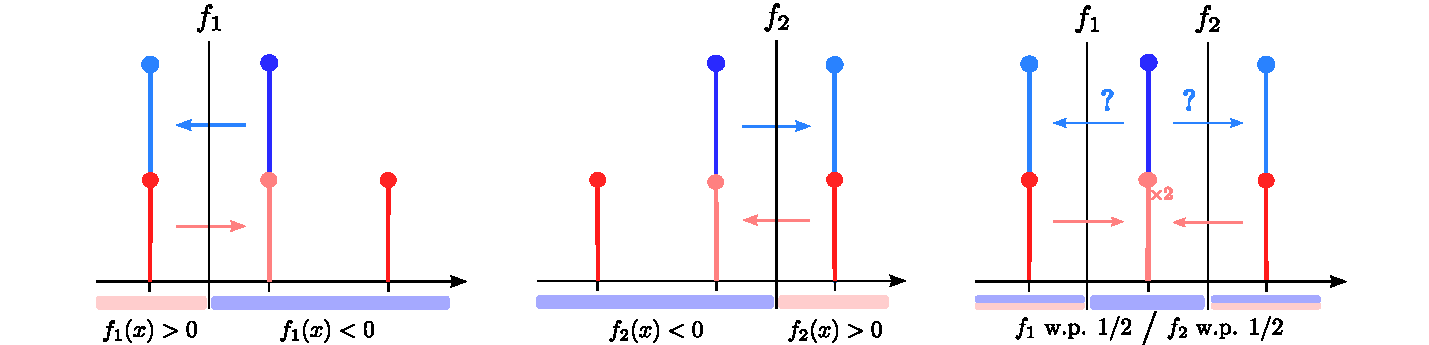
\includegraphics[width=\textwidth]{Images/Drawing-Intro-Mixte-Nash-on-a-line.pdf}   \caption{Motivating example: blue distribution represents label $-1$ and the red one, label $+1$.  The height of columns represents their mass. The red and blue arrows represent the attack on the given classifier. On left: deterministic classifiers ($f_1$ on the left, $f_2$ in the middle) for whose, the blue point can always be attacked. On right: a randomized classifier, where the attacker has a probability $1/2$ of failing, regardless of the attack it selects. }
    \label{fig:motivating_ex}
\end{figure*}
Consider the binary classification task illustrated in Figure~\ref{fig:motivating_ex}. We assume that all input-output pairs $(X,Y)$ are sampled from a distribution $\PP$ defined as follows
$$ 
\PP\left(Y =\pm 1\right)=1/2 \ \mbox{ and }\left\{
    \begin{array}{ll}
        \PP\left(X=0 \mid Y=-1\right) = 1 \\
        \PP\left(X= \pm 1 \mid Y=1\right) = 1/2 
    \end{array}
\right.
$$ 
Given access to $\PP$, the adversary aims to maximize the expected risk, but can only move each point by at most $1$ on the real line. In this context, we study two classifiers: $f_1(x) = -x -1/2$ and $f_2(x)=x-1/2$\footnote{$(X,Y) \sim \PP$ is misclassified by $f_i$ if and only if $f_i(X)Y \leq 0$}. Both $f_1$ and $f_2$ have a standard risk of $1/4$. In the presence of an adversary, the risk (\emph{a.k.a.} the adversarial risk) increases to $1$. Here, using a randomized classifier can make the system more robust. Consider $f$ where $f=f_1$ w.p. $1/2$ and $f_2$ otherwise. The standard risk of $f$ remains $1/4$ but its adversarial risk is $3/4<1$. Indeed, when attacking $f$, any adversary will have to choose between moving points from $0$ to $1$ or to $-1$. Either ways, the attack only works half of the time; hence an overall adversarial risk of $3/4$. Furthermore, if $f$ knows the strategy the adversary uses, it can always update the probability it gives to $f_1$ and $f_2$ to get a better (possibly deterministic) defense. For example, if the adversary chooses to always move $0$ to $1$, the classifier can set $f=f_1$ w.p. $1$ to retrieve an adversarial risk of $1/2$ instead of $3/4$. %In other words, if the adversary can only use a deterministic attack, then there exists no equilibrium in the game.

Now, what happens if the adversary can use randomized strategies, meaning that for each point it can flip a coin before deciding where to move? In this case, the adversary could decide to move points from $0$ to $1$ w.p. $1/2$ and to $-1$ otherwise. This strategy is still optimal with an adversarial risk of $3/4$ but now the classifier cannot use its knowledge of the adversary's strategy to lower the risk. We are in a state where neither the adversary nor the classifier can benefit from unilaterally changing its strategy. In the game theory terminology, this state is called a Mixed Nash equilibrium. %Previous works studying adversarial examples from the scope of game theory investigated the existence of Mixed Nash equilibria in restricted settings where the adversary can by reduced to a set of parameters~\citep{7533509,DBLP:journals/corr/abs-1906-02816,bose2021adversarial}. But, as pointed out in \citep{pinot2020randomization} and \citep{pydi2019adversarial}, studying the existence of a Mixed Nash equilibrium in a more general framework is a challenging open problem. In the present paper we tackle the following question.

\subsection{General setting}
Let us consider a loss function: $\loss:\Theta\times (\XX\times\YY)\to [0,\infty)$ satisfying the following set of assumptions.
\begin{assump}[Loss function]
\label{ass:loss}
1) The loss function $\loss$ is a non negative Borel measurable function. 2) For all $\theta\in\Theta$, $\loss(\theta,\cdot)$ is upper-semi continuous. 3) There exists $M>0$ such that for all $\theta\in\Theta$, $(x,y)\in\XX\times\YY$, $0\leq \loss(\theta,(x,y))\leq M$.
\end{assump}
It is usual to assume upper-semi continuity when studying optimization over distributions~\citep{villani2003topics,blanchet2019quantifying}. Furthermore, considering bounded (and positive) loss functions is also very common in learning theory~\citep{bartlett2002rademacher} and is not restrictive. 

In the adversarial examples framework, the loss of interest is the $0/1$ loss, for whose surrogates are misunderstood  and is the object of Chapter~\ref{chap:calibration}; hence it is essential that a $0/1$ loss satisfies Assumption~\ref{ass:loss}. In the binary classification setting (\emph{i.e.} $\YY=\{-1,+1\}$) a possible $0/1$ loss writes $\loss_{0/1}(\theta,(x,y)) = \mathbf{1}_{yf_\theta(x)\leq 0}$. Then, assuming that for all $\theta$, $f_\theta(\cdot)$ is continuous and for all $x$, $f_\cdot(x)$ is continuous, the $0/1$ loss satisfies Assumption~\ref{ass:loss}. In particular, it is the case for neural networks with continuous activation functions.


\subsection{Measure Theoretic Lemmas}

We first recall and prove some important lemmas about measure theory.
\begin{lemma}[Fubini's theorem]
\label{lem:fubini}
Let $\loss:\Theta\times(\XX\times\YY)\rightarrow [0,\infty)$ satisfying Assumption~\ref{ass:loss}. Then for all $\mu\in\mathcal{M}^1_+(\Theta)$, $\int \loss(\theta,\cdot)d\mu(\theta)$ is Borel measurable; for  $\QQ\in\mathcal{M}^1_+(\XX\times\YY)$, $\int \loss(\cdot,(x,y))d\QQ(x,y)$ is Borel measurable. Moreover: $\int \loss(\theta,(x,y))d\mu(\theta)d\QQ(x,y)=\int \loss(\theta,(x,y))d\QQ(x,y)d\mu(\theta)$
\end{lemma}

\begin{lemma}
\label{lem:usc1}
Let $\loss:\Theta\times(\XX\times\YY)\rightarrow [0,\infty)$ satisfying Assumption~\ref{ass:loss}.
Then for all $\mu\in\mathcal{M}^1_+(\Theta)$, $(x,y)\mapsto\int \loss(\theta,(x,y))d\mu(\theta)$ is upper semi-continuous and hence Borel measurable.  
\end{lemma}
\begin{proof}
Let $(x_n,y_n)_n$ be a sequence of $\XX\times\YY$ converging to $(x,y)\in\XX\times\YY$.  Let $M$ be an upper bound on the loss $\loss$. For all $\theta\in\Theta$, $M-\loss(\theta,\cdot)$ is non negative and lower semi-continuous. Then by Fatou's Lemma :
\begin{align*}
   \int M-\loss(\theta,(x,y))d\mu(\theta)&\leq\int \liminf_{n\to\infty}  M-\loss(\theta,(x_n,y_n))d\mu(\theta)\\
   &\leq  \liminf_{n\to\infty}  \int M-\loss(\theta,(x_n,y_n))d\mu(\theta) 
\end{align*}

We then have: $\int M- \loss(\theta,\cdot)d\mu(\theta)$ is lower semi-continuous and then $\int \loss(\theta,\cdot)d\mu(\theta)$ is upper-semi continuous.
\end{proof}


\begin{lemma}
\label{lem:usc2}

Let $\loss:\Theta\times(\XX\times\YY)\rightarrow [0,\infty)$ satisfying Assumption~\ref{ass:loss}.
Then for all $\mu\in\mathcal{M}^1_+(\Theta)$, $\QQ\mapsto\int \loss(\theta,(x,y))d\mu(\theta)d\QQ(x,y)$ is upper semi-continuous for the weak topology of measures. 
\end{lemma}
\begin{proof}
 $-\int \loss(\theta,\cdot)d\mu(\theta) $ is lower semi-continuous from Lemma~\ref{lem:usc1}. Then $M-\int \loss(\theta,\cdot)d\mu(\theta) $ is lower semi-continuous and non negative. Letus  denote $v$ this function. Let $(v_n)_n$ be a non-decreasing sequence of continuous bounded functions such that $v_n\to v$. Let $(\QQ_k)_k$ converge weakly towards $\QQ$. Then by monotone convergence theorem:
 
 \begin{align*}
     \int vd\QQ = \lim_n \int v_nd\QQ =\lim_n \lim_k\int v_nd\QQ_k\leq \liminf_k \int vd\QQ_k
 \end{align*}
 Then $\QQ\mapsto\int vd\QQ$ is lower semi-continuous and then 
 \begin{align*}
    \QQ\mapsto\int \loss(\theta,(x,y))d\mu(\theta)d\QQ(x,y)
 \end{align*}
  is upper semi-continuous for weak topology of measures. 
 \end{proof}



% \begin{lemma}
% \label{lem:measure-sup}
% Let $\loss:\Theta\times(\XX\times\YY)\rightarrow [0,\infty)$ satisfying Assumption~\ref{ass:loss}.
% Then for all $\mu\in\mathcal{M}^1_+(\Theta)$, $(x,y)\mapsto \sup_{(x',y'),d(x,x')\leq\varepsilon,y=y'} \int \loss(\theta,(x',y'))d\mu(\theta)$ is universally measurable (i.e. measurable for all Borel probability measures). And hence the adversarial risk is well defined. 
% \end{lemma}
% \begin{proof}
% Let $\phi :(x,y)\mapsto \sup_{(x',y'),d(x,x')\leq\varepsilon,y=y'} \int \loss(\theta,(x',y'))d\mu(\theta)$. Then for $u\in\bar{\mathbb{R}}$:
% \begin{align*}
% &\left\{\phi(x,y)>u\right\}\\
% &=\text{Proj}_1\left\{((x,y),(x',y'))\mid\int \loss(\theta,(x',y'))d\mu(\theta)-c_\varepsilon((x,y),(x',y'))>u\right\}
% \end{align*}
% By Lemma~\ref{lem:usc2}: $((x,y),(x',y'))\mapsto \int \loss(\theta,(x',y'))d\mu(\theta)-c_\varepsilon((x,y),(x',y'))$ is upper-semicontinuous hence Borel measurable. So its level sets are Borel sets, and by~\citet[Proposition 7.39]{bertsekas2004stochastic}, the projection of a Borel set is analytic. And then $\left\{\phi(x,y)>u\right\}$ universally measurable thanks to~\citet[Corollary 7.42.1]{bertsekas2004stochastic}. We deduce that $\phi$ is universally measurable.
% \end{proof}



\subsection{Adversarial Risk Minimization}
The standard risk for a single classifier $\theta$ associated with the loss $\loss$ satisfying Assumption~\ref{ass:loss} writes: $\risk(\theta):=\mathbb{E}_{(x,y)\sim \PP}\left[\loss(\theta,(x,y))\right]$. Similarly, the adversarial risk of $\theta$ at level $\varepsilon$ associated with the loss $\loss$ is defined as\footnote{For the well-posedness, see Lemma~\ref{lem:measure-sup}.}
\begin{align*}
    \risk_\varepsilon(\theta):=\mathbb{E}_{(x,y)\sim \PP}\left[\sup_{x'\in\XX,~d(x,x')\leq\varepsilon}\loss(\theta,(x',y))\right].
\end{align*}
 It is clear that $\risk_0(\theta) =\risk(\theta)$ for all $\theta$. We can generalize these notions with distributions of classifiers. In other terms the classifier is then randomized according to some distribution $\mu\in\mathcal{M}^1_+(\Theta)$. A classifier is randomized if for a given input, the output of the classifier is a probability distribution.
 The standard risk of a randomized classifier $\mu$ writes $\risk(\mu) = \mathbb{E}_{\theta\sim\mu}\left[\risk (\theta)\right]$. Similarly, the adversarial risk of the randomized classifier $\mu$ at level $\varepsilon$ is\footnote{This risk is also well posed (see Lemma~\ref{lem:measure-sup}).}
\begin{align*}
    \risk_\varepsilon(\mu):=\mathbb{E}_{(x,y)\sim \PP}\left[\sup_{x'\in\XX,~d(x,x')\leq\varepsilon}\mathbb{E}_{\theta\sim\mu}\left[\loss(\theta,(x',y))\right]\right].
\end{align*}
For instance, for the $0/1$ loss, the inner maximization problem, consists in maximizing the probability of misclassification for a given pair $(x,y)$. Note that $\risk(\delta_\theta)=\risk(\theta)$ and $\risk_\varepsilon(\delta_\theta)=\risk_\varepsilon(\theta)$. In the remainder of this section, we study the adversarial risk minimization problems with randomized and deterministic classifiers and denote
\begin{align}
\label{eq:advriskmin}
    \valuerand_\varepsilon:=\inf_{\mu\in\mathcal{M}^1_+(\Theta)} \risk_\varepsilon(\mu),~\valuedet_\varepsilon:=\inf_{\theta\in\Theta} \risk_\varepsilon(\theta)
\end{align}
Note that we can show that the standard risk infima are equal :  $\valuerand_0=\valuedet_0$. 
\begin{prop}
\label{prop:eqstandardrisk}
Let $\PP$ be a Borel probability distribution on $\XX\times\YY$, and $\loss$ a loss satisfying Assumption~\ref{ass:loss}, then:
\begin{align*}
        \inf_{\mu\in\mathcal{M}^1_+(\Theta)} \risk(\mu) =\inf_{\theta\in\Theta} \risk(\theta)
\end{align*}
\end{prop}
\begin{proof}
We have $\inf_{\mu\in\mathcal{M}^1_+(\Theta)} \risk(\mu) \leq \inf_{\theta\in\Theta} \risk(\theta)$. Now, let $\mu\in\mathcal{M}^1_+(\Theta)$, then:
\begin{align*}
    \risk(\mu)= \mathbb{E}_{\theta\sim\mu}(\risk(\theta))&\geq \essinf_\mu \mathbb{E}_{\theta\sim\mu} \left(\risk(\theta)\right)\\
    &\geq\inf_{\theta\in\Theta} \risk(\theta).
\end{align*}
where $\essinf$ denotes the essential infimum.
\end{proof}
\begin{rmq}
No randomization is needed for minimizing the standard risk. Denoting $\mathcal{V}$ this common value, we also have the following inequalities for any $\varepsilon>0$, $\mathcal{V}\leq \valuerand_\varepsilon\leq \valuedet_\varepsilon$.
\end{rmq}



\subsection{Distributional Formulation of the Adversarial Risk} 

To account for the possible randomness of the adversary, we rewrite the adversarial attack problem as a convex optimization problem over distributions. Let us first introduce the set of adversarial distributions.
\begin{definition}[Set of adversarial distributions]
Let $\PP$ be a Borel probability distribution on $\XX\times\YY$ and $\varepsilon>0$. We define the set of adversarial distributions as
\begin{align*}
\mathcal{A}_{\varepsilon}&(\PP) := \left\{\QQ\in\mathcal{M}^+_1(\XX\times\YY)\mid\exists \gamma\in\mathcal{M}^+_1\left((\XX\times\YY)^2\right),\right.\\
&\left.d(x,x')\leq\varepsilon,~y=y'~~ \gamma\text{-a.s.},~\Pi_{1\sharp}\gamma=\PP,~\Pi_{2\sharp}\gamma=\QQ\right\} 
\end{align*}
where $\Pi_i$ denotes the projection on the $i$-th component, and $g_\sharp$ the push-forward measure by a measurable function $g$.
\end{definition}
An attacker that can move the initial distribution $\PP$ anywhere in $\mathcal{A}_\varepsilon(\PP)$ is not applying a point-wise deterministic perturbation as considered in the standard adversarial risk. %For every point $(x,y)$ in the support of $\PP$, the attacker is allowed to move $(x,y)$ according to a ``random mapping'' in the ball of radius $\varepsilon$, and not to a single other point $(x',y)$ like the usual attacker in adversarial attacks. 
In other words, for a point $(x,y)\sim\PP$, the attacker could choose a distribution $q(\cdot\mid(x,y))$ whose support is included in $\{(x',y')\mid d(x,x')\leq \epsilon,~y=y'\}$ from which he will sample the adversarial attack. In this sense, we say the attacker is allowed to be randomized.
% This set allows to move every single point in the support of $\PP$ and moving its mass everywhere as far as the perturbation is smaller than $\varepsilon$ and does not change the `true' label. In this problem, the attacker can then play randomized strategies to move the samples inside the balls of radius $\varepsilon$. \textcolor{red}{Pas hyper limpide je trouve}

\textbf{Link with DRO.} We immediately remark that $\mathcal{A}_\varepsilon(\PP)$ corresponds to the Wasserstein-$\infty$ set associated with
the cost
\begin{align*}
    d'((x,y),(x',y'))\mapsto \left\{
        \begin{array}{ll}
            d(x,x') & \mbox{if } y = y'\\
            +\infty & \mbox{otherwise.}
        \end{array}
    \right.
\end{align*}
Such a set can be defined from usual (not $\infty$) Wasserstein uncertainty sets:  for an arbitrary $\varepsilon>0$, we define the cost $c_\varepsilon$ as follows
\begin{align*}
c_\varepsilon((x,y),(x',y')) := \left\{
    \begin{array}{ll}
        0 & \mbox{if } d(x,x')\leq\varepsilon\mbox{ and }y = y'\\
        +\infty & \mbox{otherwise.}
    \end{array}
\right.
\end{align*}
This cost is lower semi-continuous and penalizes to infinity perturbations that change the label or move the input by a distance greater than $\varepsilon$. As Proposition~\ref{prop:wass_ball} shows, the Wasserstein ball associated with $c_\varepsilon$ is equal to $\mathcal{A}_{\varepsilon}(\PP)$.
\begin{prop}
\label{prop:wass_ball}
Let $\PP$ be a Borel probability distribution on $\XX\times\YY$ and $\varepsilon>0$ and $\eta\geq 0$, then
    $\mathcal{B}_{c_\varepsilon}(\PP,\eta) =\mathcal{A}_{\varepsilon}(\PP)$.
Moreover, $\mathcal{A}_{\varepsilon}(\PP)$ is convex and compact for the weak topology of $\mathcal{M}^+_1(\XX\times\YY)$.
\end{prop}
\begin{proof}
Let $\eta>0$. Let $\QQ\in\mathcal{A}_\varepsilon(\PP)$. There exists $\gamma\in
\mathcal{M}^+_1\left((\XX\times\YY)^2\right)$ such that, $d(x,x')\leq\varepsilon$, $y=y'$ $\gamma$-almost surely, and $\Pi_{1\sharp}\gamma=\PP$, and $\Pi_{2\sharp}\gamma=\QQ$. Then $\int c_\varepsilon d \gamma = 0\leq \eta$. Then, $W_{c_\varepsilon}(\PP,\QQ)\leq \eta$, and $\QQ\in\mathcal{B}_{c_\varepsilon}(\PP,\eta)$. Reciprocally, let $\QQ\in\mathcal{B}_{c_\varepsilon}(\PP,\eta)$. Then, since the infimum is attained in the Wasserstein definition, there exists $\gamma\in
\mathcal{M}^+_1\left((\XX\times\YY)^2\right)$ such that $\int c_\varepsilon d \gamma \leq \eta$. Since $c_\varepsilon((x,x'),(y,y'))=+\infty$ when $d(x,x')>\varepsilon$ and $y\neq y'$, we deduce that, $d(x,x')\leq\varepsilon$ and $y=y'$, $\gamma$-almost surely. Then $\QQ\in\mathcal{A}_\varepsilon(\PP)$. We have then shown that: $\mathcal{A}_\varepsilon(\PP)=\mathcal{B}_{c_\varepsilon}(\PP,\eta)$.

The convexity of $\mathcal{A}_\varepsilon(\PP)$ is  immediate from the relation with the Wasserstein uncertainty set.

Let us show first that $\mathcal{A}_\varepsilon(\PP)$ is relatively compact for the weak topology. To do so we will show that $\mathcal{A}_\varepsilon(\PP)$ is tight and apply Prokhorov theorem. Let $\delta>0$, $(\XX\times \YY,d\oplus d')$ being a Polish space, $\{\PP\}$ is tight then there exists $K_\delta$ compact such that $\PP(K_\delta)\geq1-\delta$.
Let $\Tilde{K}_\delta:=\left\{(x',y')\mid \exists (x,y)\in K_\delta,~ d(x',x)\leq\varepsilon,~y=y'\right\}$.  Recalling that $(\XX,d)$ is proper (i.e. the closed balls are compact), so $\Tilde{K}_\delta$ is compact. Moreover for $\QQ\in\mathcal{A}_\varepsilon(\PP)$, $\QQ(\Tilde{K}_\delta)\geq \PP(K_\delta)\geq 1-\delta$. And then, Prokhorov's theorem holds, and $\mathcal{A}_\varepsilon(\PP)$ is relatively compact for the weak topology.

Let us now prove that $\mathcal{A}_\varepsilon(\PP)$ is closed to conclude.  Let $(\QQ_n)_n$ be a sequence of $\mathcal{A}_\varepsilon(\PP)$ converging towards some $\QQ$ for weak topology. For each $n$, there exists $\gamma_n\in \mathcal{M}^1_+(\XX\times\YY)$ such that $d(x,x')\leq\varepsilon$ and $y=y'$ $\gamma_n$-almost surely and $\Pi_{1\sharp}\gamma_n=\PP$, $\Pi_{2\sharp}\gamma_n=\QQ_n$. $\{\QQ_n,n\geq0\}$ is relatively compact, then tight, then $\bigcup_n \Gamma_{\PP,\QQ_n}$ is tight, then relatively compact by Prokhorov's theorem. $(\gamma_n)_n\in\bigcup_n \Gamma_{\PP,\QQ_n}$, then up to an extraction,  $\gamma_n\to\gamma$. Then $d(x,x')\leq\varepsilon$ and $y=y'$ $\gamma$-almost surely, and by continuity, $\Pi_{1\sharp}\gamma=\PP$ and by continuity, $\Pi_{2\sharp}\gamma=\QQ$. And hence $\mathcal{A}_\varepsilon(\PP)$ is closed.

Finally $\mathcal{A}_\varepsilon(\PP)$ is a convex compact set for the weak topology. 
\end{proof}




% Next proposition shows that the set $\mathcal{A}_{\varepsilon}(\PP)$ satisfies interesting topological properties. See proof in Appendix~\ref{prv:a_eps}.
% \begin{prop}
% \label{prop:a_eps}
% Let $\PP$ be a Borel probability distribution on $\XX\times\YY$ and $\varepsilon>0$. $\mathcal{A}_{\varepsilon}(\PP)$ is convex and compact for the weak topology of $\mathcal{M}^+_1(\XX\times\YY)$.
% \end{prop}
Thanks to this result, we can reformulate the adversarial risk as the value of a convex problem over $\mathcal{A}_\varepsilon(\PP)$. %See proof in Appendix~\ref{prv:duality-rand}.
\begin{prop} 
\label{prop:dro_adv}
Let $\PP$ be a Borel probability distribution on $\XX\times\YY$ and $\mu$ a Borel probability distribution on $\Theta$. Let $\loss:\Theta\times(\XX\times\YY)\to [0,\infty)$ satisfying Assumption~\ref{ass:loss}. Let $\varepsilon>0$. Then:
\begin{align}
\label{eq:dro-adv}
\risk_\varepsilon(\mu)= \sup_{\QQ\in \mathcal{A}_{\varepsilon}(\PP)}\mathbb{E}_{(x',y')\sim\QQ,\theta\sim\mu}\left[\loss(\theta,(x',y'))\right].
\end{align}
The supremum is attained. Moreover $\QQ^*\in \mathcal{A}_{\varepsilon}(\PP)$ is an optimum of Problem~\eqref{eq:dro-adv} if and only if there exists $\gamma^*\in\mathcal{M}^+_1\left((\XX\times\YY)^2\right)$ such that: $\Pi_{1\sharp}\gamma^*=\PP$, $\Pi_{2\sharp}\gamma^*=\QQ^*$, $d(x,x')\leq\varepsilon$, $y=y'$ and  $\loss(x',y')=\sup_{\substack{u\in\XX,d(x,u)\leq\varepsilon}}\loss(u,y)$ $\gamma^*$-almost surely.
\end{prop}

\begin{proof}
Let $\mu\in\mathcal{M}^1_+(\Theta)$. Let us define $\Tilde{f}$ as
\begin{align*}
    \Tilde{f}:((x,y),(x',y'))\mapsto \mathbb{E}_{\theta\sim\mu}\left[\loss(\theta,(x,y))\right]-c_\varepsilon((x,y),(x',y'))\quad. 
\end{align*}
 $\Tilde{f}$ is upper-semi continuous, hence upper semi-analytic. Then, by upper semi continuity of $\mathbb{E}_{\theta\sim\mu}\left[\loss(\theta,\cdot)\right]$ on the compact $\{(x',y')\mid~d(x,x')\leq\varepsilon,y=y'\}$ and~\citep[Proposition 7.50]{bertsekas2004stochastic}, there exists a universally measurable mapping $T$ such that $\mathbb{E}_{\theta\sim\mu}\left[\loss(\theta,T(x,y))\right]=\sup_{(x',y'),~d(x,x')\leq\varepsilon,y=y'}\mathbb{E}_{\theta\sim\mu}\left[\loss(\theta,(x,y))\right]$.  Let $\QQ = T_{\sharp}\PP$, then $\QQ\in\mathcal{A}_\varepsilon(\PP)$. And then 
 \begin{align*}
      \mathbb{E}_{(x,y)\sim\PP}&\left[\sup_{(x',y'),~d(x,x')\leq\varepsilon,y=y'}\mathbb{E}_{\theta\sim\mu}\left[\loss(\theta,(x',y'))\right]\right]\\
      &\leq \sup_{\QQ\in\mathcal{A}_\varepsilon(\PP)}\mathbb{E}_{(x,y)\sim\QQ}\left[\mathbb{E}_{\theta\sim\mu}\left[\loss(\theta,(x,y))\right]\right]\quad.
\end{align*}


Reciprocally, let $\QQ\in\mathcal{A}_\varepsilon(\PP)$. There exists $\gamma\in\mathcal{M}^1_+((\XX\times\YY)^2)$, such that $d(x,x')\leq\varepsilon$ and $y=y'$ $\gamma$-almost surely, and, $\Pi_{1\sharp}\gamma=\PP$ and  $\Pi_{2\sharp}\gamma=\QQ$. Then:
$\mathbb{E}_{\theta\sim\mu}\left[\loss(\theta,(x',y'))\right]\leq\sup_{(u,v),~d(x,u)\leq\varepsilon,y=v}\mathbb{E}_{\theta\sim\mu}\left[\loss(\theta,(u,v))\right]$ $\gamma$-almost surely. Then, we deduce that:
\begin{align*}
    \mathbb{E}_{(x',y')\sim\QQ}&\left[\mathbb{E}_{\theta\sim\mu}\left[\loss(\theta,(x',y'))\right]\right]\\
    & =     \mathbb{E}_{(x,y,x',y')\sim\gamma}\left[\mathbb{E}_{\theta\sim\mu}\left[\loss(\theta,(x',y'))\right]\right] \\
    &\leq\mathbb{E}_{(x,y,x',y')\sim\gamma}\left[\sup_{(u,v),~d(x,u)\leq\varepsilon,y=v}\mathbb{E}_{\theta\sim\mu}\left[\loss(\theta,(u,v))\right]\right]\\
    &\leq\mathbb{E}_{(x,y)\sim\PP}\left[\sup_{(u,v),~d(x,u)\leq\varepsilon,y=v}\mathbb{E}_{\theta\sim\mu}\left[\loss(\theta,(u,v))\right]\right]
\end{align*}

Then we deduce the expected result:
\begin{align*}
\risk_\varepsilon(\mu)= \sup_{\QQ\in\mathcal{A}_\varepsilon(\PP)}\mathbb{E}_{(x,y)\sim\QQ}\left[\mathbb{E}_{\theta\sim\mu}\left[\loss(\theta,(x,y))\right]\right]
\end{align*}
Let us show that the optimum is attained. $\QQ\mapsto\mathbb{E}_{(x,y)\sim\QQ}\left[\mathbb{E}_{\theta\sim\mu}\left[\loss(\theta,(x,y))\right]\right]$ is upper semi continuous by Lemma~\ref{lem:usc2} for the weak topology of measures, and $\mathcal{A}_\varepsilon(\PP)$ is compact by Proposition~\ref{prop:wass_ball}, then by Prop. 7.32 from ~\citep{bertsekas2004stochastic}, the supremum is attained for a certain $\QQ^*\in\mathcal{A}_\varepsilon(\PP)$. 

\end{proof}

The adversarial attack problem is a DRO problem for the cost $c_\varepsilon$.
Proposition~\ref{prop:dro_adv} means that, against a fixed classifier $\mu$, the randomized attacker that can move the distribution in $\mathcal{A}_\varepsilon(\PP)$ has exactly the same power as an attacker that moves every single point $x$ in the ball of radius $\varepsilon$.  By Proposition~\ref{prop:dro_adv}, we also  deduce that the adversarial risk can be casted as a linear optimization problem over distributions.

\begin{rmq}
  In a recent work,~\citep{pydi2019adversarial} proposed a similar adversary using Markov kernels but left as an open question the link with the classical adversarial risk, due to measurability issues. Proposition~\ref{prop:dro_adv} solves these issues. The result is similar to~\citep{blanchet2019quantifying}. Although we believe its proof might be extended for infinite valued costs,~\citep{blanchet2019quantifying} did not treat that case. We provide an alternative proof in this special case. 
\end{rmq}


 %In the next section we show how Proposition~\ref{prop:dro_adv} helps casting the adversarial risk minimization problem as a game between the classifier and the attacker for which we study the Nash equilibria.

% \paragraph{Link with distributionally robust optimization (DRO). } The optimization problem over $\mathcal{A}_\varepsilon(\PP)$ is very close to a DRO problem ~\citep{blanchet2019quantifying}. 
% When $(\mathcal{Z},d)$ a Polish space and $c:\mathcal{Z}^2\rightarrow\mathbb{R}^+\cup\{+\infty\}$ be a lower semi-continuous function, for $\PP,\QQ\in\mathcal{M}^+_1(\mathcal{Z})$ , the primal Optimal Transport problem is defined as:
% \begin{align*}
%   W_c(\PP,\QQ):=\inf_{\gamma\in\Gamma_{\PP,\QQ}}  \int_{\mathcal{Z}^2} c(z,z')d\gamma(z,z')
% \end{align*}
% with $\Gamma_{\PP,\QQ}:=\left\{\gamma\in\mathcal{M}^+_1(\mathcal{Z}^2)\mid~\Pi_{1\sharp}\gamma = \PP,~\Pi_{2\sharp}\gamma = \QQ \right\}$. When $\delta>0$ and for $\PP\in\mathcal{M}^+_1(\mathcal{Z})$, the associated Wasserstein uncertainty set is defined as: 
% \begin{align*}
%     \mathcal{B}_{c}(\PP,\delta) := \left\{\QQ\in \mathcal{M}^+_1(\mathcal{Z})\mid W_c(\PP,\QQ)\leq \delta\right\}
% \end{align*}
% A DRO problem is a linear optimization problem over Wasserstein uncertainty sets. We can show that $\mathcal{A}_{\varepsilon}(\PP)$ is actually a Wasserstein uncertainty set for a well-suited cost on $(\XX\times\YY)^2$. For $\varepsilon$, we define $c_\varepsilon$ the cost defined as $c_\varepsilon((x,y),(x',y')) = d(x,x')$ if $d(x,x')\leq\varepsilon$ and $y = y'$, and $+\infty$ otherwise. The cost for perturbations that changing the label and the input by a distance greater than $\varepsilon$ would be infinite. Next proposition link the Wasserstein ball associated with $c_\varepsilon$ and $\mathcal{A}_{\varepsilon}(\PP)$.
% \begin{prop}
% Let $\PP$ be a Borel probability distribution on $\XX\times\YY$ and $\varepsilon>0$ and $\delta>\varepsilon$, then:
% \begin{align*}
%     \mathcal{B}_{c_\varepsilon}(\PP,\delta) =\mathcal{A}_{\varepsilon}(\PP)
% \end{align*}
% \end{prop}
% One may have thought to apply directy Theorem 1 from~\citep{blanchet2019quantifying} to prove Proposition~\ref{prop:dro_adv}; however, the result holds for real-valued costs (i.e. $<\infty$). We believe it can be extended to infinite valued costs, but it is out of the scope of this paper. 
% \begin{prop} 
% \label{prop:dro_adv}
% Let $\PP$ be a Borel probability distribution on $\XX\times\YY$ and $\mu$ a Borel probability distribution on $\Theta$. Let $l:\Theta\times(\XX\times\YY)\to [0,+\infty]$ satisfying Assumption~\ref{ass:loss}. Let $\varepsilon>0$. Then:
% \begin{align*}
% \risk^\epsilon(\mu)= \sup_{\QQ\in \mathcal{A}_{\varepsilon}(\PP)}\mathbb{E}_{(x',y')\sim\QQ,\theta\sim\mu}\left[\loss(\theta,(x',y'))\right]
% \end{align*}
% \begin{align*}
% \mathbb{E}_{(x,y)\sim \PP}\left[\sup_{\substack{u\in\XX,\\d(x,u)\leq\varepsilon}}l(u,y)\right] = \sup_{\QQ\in \mathcal{A}_{\varepsilon}(\PP)}\mathbb{E}_{(x',y')\sim\QQ}\left[\loss(x',y')\right]
% \end{align*}
% The supremum is attained. Moreover $\QQ^*\in \mathcal{A}_{\varepsilon}(\PP)$ is an optimum if and only if there exists $\gamma^*\in\mathcal{M}^+_1\left((\XX\times\YY)^2\right)$ such that: $\Pi_{1\sharp}\gamma^*=\PP$, $\Pi_{2\sharp}\gamma^*=\QQ^*$, $d(x,x')\leq\varepsilon$, $y=y'$ and  $l(x',y')=\sup_{\substack{u\in\XX,d(x,u)\leq\varepsilon}}l(u,y)$ $\gamma^*$-almost surely.
% \end{prop}


% say that the program is linear blabla + link with latest pydi
% One can also recast the adversarial problem as an infinite linear problem:
% \begin{align*}
%   \risk^\epsilon(\mu) = \sup_{\gamma\in \Tilde{\mathcal{A}}_{\varepsilon}(\PP)}\mathbb{E}_{(x,y,x',y')\sim\gamma}\left[\loss(x',y')\right]
% \end{align*}

% where 
% \begin{align*}
% \Tilde{\mathcal{A}}_{\varepsilon}&(\PP) := \left\{\gamma\in\mathcal{M}^+_1\left((\XX\times\YY)^2\right)\mid~\Pi_{1\sharp}\gamma=\PP\right.\\
% &\left.\int \delta\{d(x,x')\leq\varepsilon,~y=y'\}d\gamma(x,y,x'y')=0\right\}
% \end{align*}
% with $\delta$ is the indicator function. Remark that $\mathcal{A}_{\varepsilon}(\PP)=\Pi_{2\sharp}\Tilde{\mathcal{A}}_{\varepsilon}(\PP)$

% \paragraph{A primal-dual formulation of risk minimization.}Let $\mu\in\mathcal{M}^1_+(\Theta)$ a possibly randomized classifier. Thanks to Proposition~\ref{prop:dro_adv}, we have that for $\varepsilon>0$:
% \begin{align*}
%     \risk^\varepsilon(\mu)=\sup_{\QQ\in\mathcal{A}_{\varepsilon}(\PP)}\mathbb{E}_{(x,y)\sim\QQ,\theta\sim\mu}\left[\loss(\theta,(x,y))\right]
% \end{align*}
% Following the definition of the risk minimization objective,  one can define the dual of this problem for randomized classifiers:
% \begin{align}
%     \sup_{\QQ\in\mathcal{A}_{\varepsilon}(\PP)}\inf_{\mu\in\mathcal{M}^1_+(\Theta)}\mathbb{E}_{(x,y)\sim\QQ,\theta\sim\mu}\left[\loss(\theta,(x,y))\right]
% \label{eq:dual_pb}
% \end{align}
% and its analog for deterministic classifiers:
% \begin{align*}
%     \sup_{\QQ\in\mathcal{A}_{\varepsilon}(\PP)}\inf_{\theta\in\Theta}\mathbb{E}_{(x,y)\sim\QQ}\left[\loss(\theta,(x,y))\right]
% \end{align*}
% Then, one can notice that the dual problems for deterministic and randomized classifiers are equivalent\footnote{See Appendix XXX for more details}. We denote $\dualvalue^\varepsilon$ the value of the dual problem.
% Weak duality is always satisfied:
% \begin{align}
% \label{eq:weak_duality}
% \dualvalue^\varepsilon\leq \valuerand^\varepsilon\leq \valuedet^\varepsilon
% \end{align}
% We will show in the next section, that, under Assumption~\ref{ass:loss}, strong duality always holds for this min-max problem.


% \begin{definition}[Optimal transport problem] Let $(\mathcal{Z},d)$ be a Polish space. Let $c:\mathcal{Z}^2\rightarrow\mathbb{R}^+\cup\{+\infty\}$ be a lower semi-continuous function. For $\PP,\QQ\in\mathcal{M}^+_1(\mathcal{Z})$, the primal optimal transport problem is defined as:
% \begin{align*}
%   W_c(\PP,\QQ):=\inf_{\gamma\in\Gamma_{\PP,\QQ}}  \int_{\mathcal{Z}^2} c(z,z')d\gamma(z,z')
% \end{align*}
% with $\Gamma_{\PP,\QQ}:=\left\{\gamma\in\mathcal{M}^+_1(\mathcal{Z}^2)\mid~\Pi_{1\sharp}\gamma = \PP,~\Pi_{2\sharp}\gamma = \QQ \right\}$ 
% \end{definition}

% We now define the Wasserstein uncertainty set.
% \begin{definition}[Wasserstein uncertainty set]Let $(\mathcal{Z},d)$ be a Polish space. Let $c:\mathcal{Z}^2\rightarrow\mathbb{R}^+\cup\{+\infty\}$ be a lower semi-continuous function. For $\PP\in\mathcal{M}^+_1(\mathcal{Z})$ and $\delta>0$, we define the Wasserstein uncertainty set:
% \begin{align*}
%     \mathcal{B}_{c}(\PP,\delta) := \left\{\QQ\in \mathcal{M}^+_1(\mathcal{Z})\mid W_c(\PP,\QQ)\leq \delta\right\}
% \end{align*}

% \end{definition}
% We recall that since for all $\PP$, $\QQ\mapsto W_c(\PP,\QQ)$ is convex, the Wasserstein uncertainty sets are convex. Moreover, $\QQ\mapsto W_c(\PP,\QQ)$ is a lower semi-continuous function for the weak topology then $\mathcal{B}_{c}(\PP,\delta)$ is a closed set. Under some mild assumptions the Wasserstein uncertainty balls are compact for weak topology. See details in App. 

% We now connect this problem to that of designing adversarial attacks for a given classification task. Let $(\XX,d_{\XX})$ be a proper Polish metric space representing the input space. Let $\YY=\{1,\dots,K\}$ be the labels set, endowed with trivial metric  $d_{\YY}(y,y') = \mathrm{1}_{y\neq y'}$. Then the space  $(\XX\times\YY,d_\XX\oplus d_\YY)$ is a proper Polish space. We denote $c_\varepsilon$ the cost defined as $c_\varepsilon((x,y),(x',y')) = d(x,x')$ if $d(x,x')\leq\varepsilon$ and $y = y'$, and $+\infty$. The cost for perturbations that changing the label and the input by a distance greater than $\varepsilon$ would be infinite. For $\delta>\epsilon$, next proposition shows that $\mathcal{B}_{c_{\varepsilon}}(\PP,\delta)$ allows all perturbations smaller than $\epsilon$.

% \begin{prop}
% Let $\PP$ be a distribution on $\XX\times\YY$ and $\varepsilon>0$ and $\delta>\varepsilon$, then:
% \begin{align*}
% \mathcal{B}_{c_{\varepsilon}}&(\PP,\delta) = \left\{\QQ\in\mathcal{M}^+_1(\XX\times\YY)\mid\exists \gamma\in\mathcal{M}^+_1\left((\XX\times\YY)^2\right),\right.\\
% &\left.d(x,x')\leq\varepsilon,~y=y'~~ \gamma\text{-a.s.},~\Pi_{1\sharp}\gamma=\PP,~\Pi_{2\sharp}\gamma=\QQ\right\} 
% \end{align*}
% This set will be denoted $\mathcal{A}_\varepsilon(\PP)$ this set. The set $\mathcal{A}_\varepsilon(\PP)$ is a convex and compact for weak topology.
% \end{prop}
 
% \begin{prop} 
% \label{prop:dro_adv}
% Let $\PP$ be a distribution on $\XX\times\YY$. Let $l:\XX\times\YY\mapsto\mathbb{R}$ be an upper semi continuous measurable function. We suppose that $l\in L^1(\PP)$. Let $\varepsilon>0$. Then:
% \begin{align*}
% \mathbb{E}_{(x,y)\sim \PP}\left[\sup_{\substack{u\in\XX,\\d(x,u)\leq\varepsilon}}l(u,y)\right] = \sup_{\QQ\in \mathcal{A}_{\varepsilon}(\PP)}\mathbb{E}_{(x',y')\sim\QQ}\left[\loss(x',y')\right]
% \end{align*}
% The supremum is attained. Moreover $\QQ^*\in \mathcal{A}_{\varepsilon}(\PP)$ is an optimum if and only if there exists $\gamma^*\in\mathcal{M}^+_1\left((\XX\times\YY)^2\right)$ such that: $\Pi_{1\sharp}\gamma^*=\PP$, $\Pi_{2\sharp}\gamma^*=\QQ^*$, $d(x,x')\leq\varepsilon$, $y=y'$ and  $l(x',y')=\sup_{\substack{u\in\XX,d(x,u)\leq\varepsilon}}l(u,y)$ $\gamma^*$-almost surely.
% \end{prop}

% \laurent{can we prove this result without using blanchet, i think so no? It is the result of blanchet}

\section{Nash Equilibria in the Adversarial Game}
\label{sec:nash-eq}

\subsection{Adversarial Attacks as a Zero-Sum Game}

Thanks to Proposition~\ref{sec:adv-problem}, the adversarial risk minimization problem can  be seen as a two-player zero-sum game that writes as follows,
\begin{align}
    \inf_{\mu\in\mathcal{M}^1_+(\Theta)} \sup_{\QQ\in\mathcal{A}_{\varepsilon}(\PP)}\mathbb{E}_{(x,y)\sim\QQ,\theta\sim\mu}\left[\loss(\theta,(x,y))\right].
\label{eq:primal_pb}
\end{align}
In this game, the classifier's objective is to find the best distribution $\mu \in \mathcal{M}_1^+(\Theta)$ while the adversary is manipulating the data distribution. For the classifier, solving the infimum problem in Equation~\eqref{eq:primal_pb} simply amounts to solving the adversarial risk minimization problem -- Problem~\eqref{eq:advriskmin}, whether the classifier is randomized or not. Then, given a randomized classifier $\mu \in \mathcal{M}_1^+(\Theta)$, the goal of the attacker is to find a new data-set distribution $\mathbb{Q}$ in the set of adversarial distributions $\mathcal{A}_{\varepsilon}(\PP)$ that maximizes the risk of $\mu$. More formally, the adversary looks for $$\mathbb{Q} \in \argmaxB_{\QQ\in\mathcal{A}_{\varepsilon}(\PP)} \mathbb{E}_{(x,y)\sim\QQ,\theta\sim\mu}\left[\loss(\theta,(x,y))\right]. $$
In the game theoretic terminology, $\mathbb{Q}$ is also called the best response of the attacker to the classifier $\mu$.

\begin{rmq}
Note that for a given classifier $\mu$ there always exists a ``deterministic'' best response, i.e. every single point $(x,y)$ is mapped to another single point $T(x,y)$. Let $T:\XX\times\YY\to\XX\times\YY$ be defined such that for all $(x,y)\in\XX\times\YY$, $\EE_{\theta\sim\mu}\left[\loss(T(x,y))\right] = \sup_{x',~d(x,x')\leq\varepsilon}\EE_{\theta\sim\mu}\left[ L(x',y)\right]$. Thanks to Prop. 7.50 from ~\citep{bertsekas2004stochastic}, $T$ is $\PP$-measurable. Moreover, we get that $\QQ = (T,id)_\sharp \PP$ belongs to the best response to $\mu$. Therefore, $T$ is the optimal ``deterministic'' attack against the classifier $\mu$.
\end{rmq}


%The classifier cannot play a best response against the attacker since the attacker is usually unknown. Thanks to the inequality~\eqref{eq:weak_duality}, the lowest risk, the classifier can hope is $\mathcal{D}^\varepsilon$. But as seen in the motivating example, it might not been attained by a deterministic classifier. We show in this section, that randomized classifiers can approach $\mathcal{D}^\varepsilon$ arbitrary closely.

%\begin{itemize}
%    \item 3.1 0 sum game , mininmizer = jeu
%    \item in this game: classifier oblivious to the attacker -> standard setting, attacker is whitebox
%    \item 3.2 dual formulation: sup inf, attackant adaptif, and Black box attacks
%    \item 3.3 evaluating duality gap
%\end{itemize}

\subsection{Dual Formulation of the Game}

Every zero sum game has a dual formulation that allows a deeper understanding of the framework. Here, from Proposition~\ref{prop:dro_adv}, we can define the dual problem of adversarial risk minimization for randomized classifiers. This dual problem also characterizes a two-player zero-sum game that writes as follows,
\begin{align}
    \sup_{\QQ\in\mathcal{A}_{\varepsilon}(\PP)}\inf_{\mu\in\mathcal{M}^1_+(\Theta)}\mathbb{E}_{(x,y)\sim\QQ,\theta\sim\mu}\left[\loss(\theta,(x,y))\right].
\label{eq:dual_pb}
\end{align}
In this dual game problem, the adversary plays first and seeks an adversarial distribution that has the highest possible risk when faced with an arbitrary classifier. This means that it has to select an adversarial perturbation for every input $x$, without seeing the classifier first. In this case, as pointed out by the motivating example in Section~\ref{sec:motiv-ex}, the attack can (and should) be randomized to ensure maximal harm against several classifiers. Then, given an adversarial distribution, the classifier objective is to find the best possible classifier on this distribution. Let us denote $\dualvalue^\varepsilon$ the value of the dual problem. Since the weak duality is always satisfied, we get
\begin{align}
\label{eq:weak_duality}
\dualvalue_\varepsilon\leq \valuerand_\varepsilon\leq \valuedet_\varepsilon.
\end{align}
Inequalities in Equation~\eqref{eq:weak_duality} mean that the lowest risk the classifier can get (regardless of the game we look at) is $\mathcal{D}^\varepsilon$. In particular, this means that the primal version of the game, \emph{i.e.} the adversarial risk minimization problem, will always have a value greater or equal to $\mathcal{D}^\varepsilon$. As we discussed in Section~\ref{sec:motiv-ex}, this lower bound may not be attained by a deterministic classifier. As we will demonstrate in the next section, optimizing over randomized classifiers allows to approach $\mathcal{D}^\varepsilon$ arbitrary closely.

Note that, we can always define the dual problem when the classifier is deterministic, \begin{align*}
    \sup_{\QQ\in\mathcal{A}_{\varepsilon}(\PP)}\inf_{\theta\in\Theta}\mathbb{E}_{(x,y)\sim\QQ}\left[\loss(\theta,(x,y))\right].
\end{align*}


We can deduce an immediate corollary from Proposition~\ref{prop:eqstandardrisk}
that the dual problems for deterministic and randomized classifiers have the same value.
\begin{corollary}
Under Assumption~\ref{ass:loss}, the dual for randomized and deterministic classifiers are equal.
\end{corollary}


%This primal-dual formulation highlights the profound link between  game theory and adversarial examples. Indeed, the adversarial risk minimization can be seen as a zero-sum game. In this section we study the Nash equilibrium of this game in the randomized setting. \textcolor{red}{pas tres clair, en quoi c'est la formulation dual qui fait apparaitre le jeu?} %We show in the next section, that, under Assumption~\ref{ass:loss}, strong duality always holds for this min-max problem, and hence study the Nash equilibrium of the related game.
%We now define the adversarial examples game, as a zero-sum game, where one player is the attacker and the other is the classifier. We study the Nash equilibria of this game in both randomized and deterministic cases.




%\textbf{Attacker Objective.}
%Given a possibly  randomized classifier $\mu\in \mathcal{M}^1_+(\Theta)$, the goal of the attacker is to find a possibly random perturbation for each single pair $(x,y)\in \supp(\PP)$, such that this perturbation maximizes $\mathbb{E}_{\theta\sim\mu}[\loss(\theta,(x',y))]$ over $x'$ under the constraint that $d(x,x')\leq\varepsilon$. In other words, thanks to Proposition $1$, the set of best responses to $\mu$ writes
%\begin{align*}
%    \text{BR}(\mu) := \argmaxB_{\QQ\in\mathcal{A}_{\varepsilon}(\PP)} \mathbb{E}_{(x,y)\sim\QQ,\theta\sim\mu}\left[ l(\theta,(x,y))\right] 
%\end{align*}




%In a white-box setting, the adversary knows the classifier $\mu$ before attacking then he only needs to perform a best response. In the black-box setting, it is different: since the adversary does not know the classifier $\mu$, he needs to compute a solution to the sup-inf problem to get its attack the most effective. Note that in this case, the attack can be possibly random: a single point $x$ can be mapped to a distribution of attacks.



%\textbf{Classifier Objective.} In the standard adversarial examples setting, since the attacker plays after the classifier, the goal of the classifier is to find the best classifier against every possible attacks at level $\varepsilon$, i.e. solving the adversarial risk minimization problem~\eqref{eq:advriskmin}, whether the classifier is randomized or not. The classifier cannot play a best response against the attacker since the attacker is usually unknown. Thanks to the inequality~\eqref{eq:weak_duality}, the lowest risk, the classifier can hope is $\mathcal{D}^\varepsilon$. But as seen in the motivating example, it might not been attained by a deterministic classifier. We show in this section, that randomized classifiers can approach $\mathcal{D}^\varepsilon$ arbitrary closely.

\subsection{Nash Equilibria for Randomized Strategies}

In the adversarial examples game, a Nash equilibrium is a couple $(\mu^*,\QQ^*)\in\mathcal{M}^1_+(\Theta)\times\mathcal{A}_\varepsilon(\PP)$ where both the classifier and the attacker have no incentive to deviate unilaterally from their strategies $\mu^*$ and $\QQ^*$. More formally, $(\mu^*,\QQ^*)$ is a Nash equilibrium of the adversarial examples game if $(\mu^*,\QQ^*)$ is a saddle point of the objective function $$(\mu,\QQ)\mapsto \mathbb{E}_{(x,y)\sim\QQ,\theta\sim\mu}\left[\loss(\theta,(x,y))\right].$$ Alternatively, we can say that $(\mu^*,\QQ^*)$ is a Nash equilibrium if and only if $\mu^*$ solves the adversarial risk minimization problem -- Problem~\eqref{eq:advriskmin}, $\QQ^*$ the dual problem -- Problem~\eqref{eq:duality}, and $\mathcal{D}^\varepsilon=\mathcal{V}_{rand}^\varepsilon$. In our problem, $\QQ^*$ always exists but it might not be the case for $\mu^*$. Then for any $\delta>0$, we say that  $(\mu_\delta,\QQ^*)$ is a $\delta$-approximate Nash equilibrium if $\QQ^*$ solves the dual problem and $\mu_\delta$ satisfies $\mathcal{D}^\varepsilon\geq\risk_\varepsilon(\mu_\delta)-\delta$. 
% \begin{align*}
%     \text{BR}(\QQ) := \argmaxB_{\mu\in\mathcal{A}_{\varepsilon}(\PP)} \int l(\theta,(x,y))d\QQ(x,y)d\mu(\theta)
% \end{align*}

% \begin{align*}
%     \inf_{\theta\in\Theta} \sup_{\QQ\in \mathcal{A}_{\varepsilon}(\PP))} \mathbb{E}_{z\sim\QQ }\left[\loss(\theta,z)\right]:=\int l(\theta,z)d\QQ(z)
% \end{align*}
% where: 
% \begin{align*}
%     \mathcal{A}_{\varepsilon}(\PP)) := \left\{\QQ\in \mathcal{M}^+_1(\mathcal{Z})\text{ s.t. } D(\PP,\QQ)\leq \varepsilon\right\}
% \end{align*}

% We will study:

% \begin{align*}
%     \inf_{\mu\in \mathcal{M}^+_1(\Theta)} \sup_{\QQ\in \mathcal{A}_{\varepsilon}(\PP))} \mathbb{E}_{\theta \sim \mu, z\sim\QQ }\left[\loss(\theta,z)\right] \\
%     =\int l(\theta,z)d\mu(\theta)d\QQ(z):=L(\mu,\QQ)
% \end{align*}

%Meyer{generalise to any sub convex set of the set of distributions of $\Theta$}

We now state our main result: the existence of approximate Nash equilibria in the adversarial examples game when both the classifier and the adversary can use randomized strategies. More precisely, we demonstrate that the duality gap between the adversary and the classifier problems is zero, which gives as a corollary the existence of Nash equilibria. 

\begin{thm}
\label{thm:duality-rand}
Let $\PP\in\mathcal{M}^1_+(\XX\times\YY)$. Let $\varepsilon>0$. Let $\loss:\Theta\times(\XX\times\YY)\to [0,\infty)$ satisfying Assumption~\ref{ass:loss}. %Let assume that for all $\mu\in\mathcal{M}^1_+(\Theta)$ and $(x,y)\in\XX\times\YY$, $l(\cdot,(x,y))$ is $\mu$-measurable.
Then strong duality always holds in the randomized  setting:
\begin{align}
 \label{eq:duality}\inf_{\mu\in \mathcal{M}^+_1(\Theta)} \max_{\QQ\in \mathcal{A}_{\varepsilon}(\PP)} \mathbb{E}_{\theta \sim \mu, (x,y)\sim\QQ }\left[\loss(\theta,(x,y))\right]\\
=
\nonumber\max_{\QQ\in \mathcal{A}_{\varepsilon}(\PP)}\inf_{\mu\in \mathcal{M}^+_1(\Theta)}  \mathbb{E}_{\theta \sim \mu, (x,y)\sim\QQ }\left[\loss(\theta,(x,y))\right]
\end{align}
The supremum is always attained. If $\Theta$ is a compact set, and for all $(x,y)\in\XX\times\YY$, $\loss(\cdot,(x,y))$ is lower semi-continuous, the infimum is also attained.
\end{thm}


\begin{proof}
$\mathcal{A}_\varepsilon(\PP)$, endowed with the weak topology of measures, is a Hausdorff compact convex space, thanks to Proposition~\ref{prop:wass_ball}. Moreover, $\mathcal{M}^1_+(\Theta)$ is clearly convex and $(\QQ,\mu)\mapsto \int \loss d\mu d\QQ$ is bilinear, hence concave-convex. Moreover thanks to Lemma~\ref{lem:usc2}, for all $\mu$, $\QQ\mapsto \int \loss d\mu d\QQ$ is upper semi-continuous. Then Fan's theorem applies and strong duality holds.
\end{proof}
 \begin{corollary}
\label{cor:nash-eq}
Under Assumption~\ref{ass:loss}, for any $\delta>0$, there exists a $\delta$-approximate Nash-Equibilrium $(\mu_\delta,\QQ^*)$. Moreover, if the infimum is attained, there exists a Nash equilibrium $(\mu^*,\QQ^*)$ to the adversarial examples game.
\end{corollary}



\cite{bose2021adversarial} mentioned a particular form of Theorem~\ref{thm:duality-rand} for convex cases.  It is still a direct corollary of Fan's theorem. This theorem can be stated as follows: 
\begin{thm}Let $\PP\in\mathcal{M}^1_+(\XX\times\YY)$, $\varepsilon>0$ and $\Theta$ a convex set. Let $\loss$ be a loss satisfying Assumption~\ref{ass:loss}, and also, $(x,y)\in\XX\times\YY$, $\loss(\cdot,(x,y))$ is a convex function, then we have the following:
\begin{align*}
\inf_{\theta\in\Theta} \sup_{\QQ\in \mathcal{A}_{\varepsilon}(\PP)} \mathbb{E}_{ \QQ }\left[\loss(\theta,(x,y))\right]
=
\sup_{\QQ\in \mathcal{A}_{\varepsilon}(\PP)}\inf_{\theta\in \Theta}  \mathbb{E}_{\QQ }\left[\loss(\theta,(x,y))\right]
\end{align*}
The supremum is always attained. If $\Theta$ is a compact set then, the infimum is also attained.
\end{thm}


Theorem~\ref{thm:duality-rand} shows that $\mathcal{D}^\varepsilon=\mathcal{V}_{rand}^\varepsilon$. From a game theoretic perspective, this means that the minimal adversarial risk for a randomized classifier against any attack (primal problem) is the same as the maximal risk an adversary can get by using an attack strategy that is oblivious to the classifier it faces (dual problem). This suggests that playing randomized strategies for the classifier could substantially improve robustness to adversarial examples.
%Second, Corollary~\ref{cor:nash-eq} says that there always exists a randomized classifier that gets arbitrarily close this minimal adversarial risk. Hence, if we can design an algorithm that efficiently learn this classifier, we will get improve adversarial robustness over classical deterministic defenses. 
In the next section, we will design an algorithm that efficiently learn a randomized classifier and show improved adversarial robustness over classical deterministic defenses.


\begin{rmq}
Theorem~\ref{thm:duality-rand} remains true if one replaces $\mathcal{A}_\varepsilon(\PP)$ with any other Wasserstein compact uncertainty sets (see~\citep{yue2020linear} for conditions of compactness). 
\end{rmq}

%Meyer{Add discrete case also}
% \paragraph{Case of $0/1$ loss.} The $0/1$ loss is particularly interesting in adversarial attacks since in this case the goal of the attacker would be to maximize the probability of misclassification. We can prove that our duality result also holds for the $0/1$ loss. 

% For $\theta\in\Theta$, we define $f_\theta:x\in\XX\mapsto (f_\theta(x)_1,\dots,f_\theta(x)_K)\in\mathbb{R}^K$ such that the predicted class is $y\in\YY$ if and only if: $f_\theta(x)_y>\max_{i\neq y} f_\theta(x)_i$. The corresponding $0/1$ loss is then: 
% \begin{align*}
% l(\theta,(x,y))=\mathbf{1}_{f_\theta(x)_y\leq\max_{i\neq y} f_\theta(x)_i}
% \end{align*}

% Assuming that for all $\theta$, $f_\theta(\cdot)$ is continuous, and that for all $\mu\in\mathcal{M}^1_+(\Theta)$ and $(x,y)\in\XX\times\YY$, $l(\cdot,(x,y))$ is $\mu$-measurable (for instance, for all $x\in\XX$, $f_{\cdot}(x)$ is continuous),  then the duality result~\eqref{eq:duality} holds for the $0/1$ loss. However the existence of a minimizing distribution $\mu^*\in\mathcal{M}^1_+(\Theta)$ is not guaranteed. See Appendix XXX for more details.
% \begin{prop}Let $\lambda>0$. For all $\theta\in \Theta$, $f_\theta:\XX\mapsto \mathbb{R}^k$. be classifier 
% \begin{align*}
% \sigma_\lambda(\theta,(x,y)) =\left(1+\exp\left\{-\lambda\left(f_\theta^y(x)-\max_{i\neq y}f_\theta^i(x)\right)\right\}\right)^{-1}
% \end{align*}
% \end{prop}






% \paragraph{Example where randomization is needed}Let now exhibit a simple example where randomization is needed. We assume that $\XX = \mathbb{R}$ and $\YY=\{-1,1\}$. Let assume the following distribution $\PP$: $Y = 1$ with probability $1/2$ and $-1$ with probability $1/2$. Conditionally to $Y=1$, $X$ always equals $0$ and conditionally to $Y=-1$, $X=1$ with probability $1/2$ and $-1$ otherwise.

% We assume that $d_\XX(x,x') =\lvert x-x'\rvert$. We now fix $\varepsilon=1$. Let consider the $0/1$ loss: $l(f,(x,y)) =\mathbf{1}_{f(x)\neq y}$.

% In this example, every Bayes optimal classifier have a zero natural risk, but the its adversarial risk is actually equal to $1$. Let now reduce the hypothesis class to two classifiers: $f_1(x) = \sign\left\{x\leq 1/2\right\}$ and $f_2(x) = \sign\left\{x\geq -1/2\right\}$. Then for $i=1,2$, $\risk(f_i)=1/4$ and $\risk(f_i)=3/4$. Let now define the randomized classifier $f=f_1$ with probability $1/2$ and $f_2$ with probability $1/2$. In this case we have $\risk(f)=1/4$ and $\risk(f)=1/2$.


% \section{todo}
% \begin{itemize}

%     \item unicity of Nash equilbrium?  no a priori
%     \item statistical study of the nash equilibrium
%     \item big part: algo...
% \end{itemize}



\section{Finding the Optimal Classifiers}
\label{sec:algo}

\subsection{An Entropic Regularization}
\label{sec:entropic-reg}


% From now on, we focus on finite class of classifiers. Let $\Theta = \{\theta_1,\dots,\theta_K\}$, we aim to learn the optimal mixture of classifiers in this case. The adversarial risk  is defined as:
% \begin{align*}
%     \risk^\varepsilon(\lambda)=\mathbb{E}_{(x,y)\sim \PP}\left[\sup_{x'\in\mathcal{X},~d(x,x')\leq\varepsilon}\sum_{k=1}^K\lambda_kl(\theta_k,(x',y))\right]
% \end{align*}
% for $\lambda\in\Delta_K: = \{\lambda\in\mathbb{R}_+^K~\mathrm{s.t.}~\sum_{i=1}^K\lambda_i=1\}$, the probability simplex of $\mathbb{R}^K$. One can notice $\risk^\varepsilon(\cdot)$ is a continuous convex function, hence $\min_{\lambda\in\Delta_K}\risk^\varepsilon(\lambda)$ is attained for a certain $\lambda^*$. Then, thanks to Corollary XXX, there always exists a Nash equilbrium to the advarsarial game when $\Theta$ is finite. In this section, we present two algorithms to learn the find the optimum of the adversarial risk minimization problem.
% \subsection{Algorithm}
% The first algorithm we present is inspired from~\citep{sinha2017certifying} and the convergence of projected sub-gradient methods CITE. The computation of the inner supremum problem is usually NP-hard~\footnote{See App XXX for details.}, but one may assume the existence of an approximate oracle to this supremum. The algorithm is presented in Algorithm~\ref{algo:duchi}. We get the following guarantees on this algorithm. See proof in Appendix XXX.
% \begin{prop}
% Let $\PP\in\mathcal{M}^1_+(\mathcal{X}\times\mathcal{Y})$. Let $l:\Theta\times(\mathcal{X}\times\mathcal{Y})\to [0,\infty)$ satisfying Assumption~\ref{ass:loss}. Then, Algorithm~\ref{algo:duchi} satisfies:  
% \begin{align*}
%     \min_{t\in[T]}\risk^\varepsilon(\lambda_t)-\risk^\varepsilon(\lambda^*)\leq2\delta+ 2\sqrt{\frac{M}{T}}
%     % \delta\sqrt{K}+ \frac{M\sum_{t=1}^T \eta_t^2+\rVert\lambda_0-\lambda^*\lVert^2}{\sum_{t=1}^T\eta_t}
% \end{align*}
% % In particular for $\eta_t =\frac{\eta}{t^{1/2}}$, we get: $\min_{t\in[T]}\risk^\varepsilon(\lambda_t)-\risk^\varepsilon(\lambda^*)\in O\left(\delta+\frac{\log T}{\sqrt{T}}\right)$
% \end{prop}
% \begin{algorithm}[H]
% \SetAlgoLined
%  $\lambda_0 = \frac{\mathbf{1}_K}{K}; T;~\eta = \sqrt{\frac{4}{MT}}$\\
%  \For{$t=1,\dots,T$}{

%   $\Tilde{\QQ}$ s.t. $\exists\QQ^*\in\mathcal{A}_\varepsilon(\PP)$,  $\mathbb{E}_{\QQ^*,\lambda}(l(\theta_k,(x,y)))= \max_{\QQ\in \mathcal{A}_\varepsilon(\PP)}\mathbb{E}_{\QQ,\lambda}(l(\theta_k,(x,y)))$ and for all $k\in[K]$, $\lvert\mathbb{E}_{\Tilde{\QQ}}(l(\theta_k,(x,y)))-\mathbb{E}_{\QQ^*}(l(\theta_k,(x,y))) \rvert\leq\delta$\\
  
%   $g_t=\left(\mathbb{E}_{\Tilde{\QQ}}(l(\theta_1,(x,y)),\dots,\mathbb{E}_{\Tilde{\QQ}}(l(\theta_K,(x,y))\right)^T$\\
%   $\lambda_t = \Pi_{\Delta_K}\left(\lambda_{t-1}-\eta g_t\right)$
%   }
%  \caption{Mixture optimization by PGD}
 
%  \label{algo:duchi}

% \end{algorithm}
% \subsection{Entropic regularization}
Let $\{(x_i,y_i)\}_{i=1}^\numsamples$ samples independently drawn from $\PP$ and denote  $\widehat{\mathbb
{P}}:=\frac{1}{\numsamples}\sum_{i=1}^\numsamples \delta_{(x_i,y_i)}$ the associated empirical distribution. %In fact for such distribution we have a simple characterization of the set  of adversarial distributions which is:
% \begin{align*}
%     \mathcal{A}_{\varepsilon}&(\widehat{\mathbb
% {P}})=\Big\{\QQ~|\exists \QQ_1,\dots,\QQ_N\in\mathcal{M}_{+}(\mathcal{X}\times\mathcal{Y}),\QQ=\sum_{i=1}^N \QQ_i,\\
% & \int_{\mathcal{X}\times\mathcal{Y}}d\QQ_i=\frac{1}{N},~\int c_{\varepsilon}((x_i,y_i),\cdot)d\QQ_i=0\Big\}.
% \end{align*}
% where 
% \begin{align*}
% \delta_{B((x_i,y_i),\varepsilon)}(x,y) = \left\{
%     \begin{array}{ll}
%         0 & \mbox{if } d(x_i,x)\leq\varepsilon\mbox{ and }y_i = y\\
%         +\infty & \mbox{otherwise.}
% %     \end{array}
% % \right.
% % \end{align*}
% Therefore by denoting
% \begin{align*}
%     \Gamma_{\varepsilon}&(\widehat{\mathbb
%  {P}})=\Big\{(\QQ_1,\dots,\QQ_N)\mid\lvert \QQ_i\rvert =\frac{1}{N},~\int c_{\varepsilon}((x_i,y_i),\cdot)d\QQ_i=0\Big\}
% \end{align*}
% the problem of interest can be written as
% \begin{align*}
% \inf_{\mu\in \mathcal{M}^+_1(\Theta)}\sup_{(Q_1,\dots,Q_N)\in\Gamma_{\varepsilon}(\widehat{\mathbb
% {P}})}\sum_{i=1}^N\mathbb{E}_{(x,y)\sim Q_i,\theta \sim \mu}\left[\loss(\theta,(x,y))\right]
% \end{align*}
One can show the adversarial empirical risk minimization can be casted as:
\begin{align*}
\widehat{\mathcal{R}}_{adv}^{\varepsilon,*}:=\inf_{\mu\in \mathcal{M}^+_1(\Theta)}\sum_{i=1}^\numsamples\sup_{\QQ_i\in\Gamma_{i,\varepsilon}}\mathbb{E}_{(x,y)\sim \QQ_i,\theta \sim \mu}\left[\loss(\theta,(x,y))\right]
\end{align*}
where $\Gamma_{i,\varepsilon}$ is defined as : 
\begin{align*}
    \Gamma_{i,\varepsilon}:=\Big\{\QQ_i\mid~\int d\QQ_i=\frac{1}{\numsamples},~\int c_{\varepsilon}((x_i,y_i),\cdot) d\QQ_i=0\Big\}.
\end{align*}
\begin{prop}
    Let $\hat{\PP}:=\frac1N\sum_{i=1}^N \delta_{(x_i,y_i)}$. Let $l$ be a loss satisfying Assumption~\ref{ass:loss}. Then we have:
    \begin{align*}
    \frac{1}{N}\sum_{i=1}^N\sup_{x,~d(x,x_i)\leq\varepsilon}\mathbb{E}_{\theta \sim \mu}\left[l(\theta,(x,y))\right]=\sum_{i=1}^N\sup_{\QQ_i\in\Gamma_{i,\varepsilon}}\mathbb{E}_{(x,y)\sim \QQ_i,\theta \sim \mu}\left[l(\theta,(x,y))\right]
    \end{align*}
    where $\Gamma_{i,\varepsilon}$ is defined as : 
    \begin{align*}
        \Gamma_{i,\varepsilon}:=\Big\{\QQ_i\mid~\int d\QQ_i=\frac{1}{N},~\int c_{\varepsilon}((x_i,y_i),\cdot) d\QQ_i=0\Big\}.
    \end{align*}\end{prop}
    
    \begin{proof}
    This proposition is a direct application of Proposition~\ref{prop:dro_adv} for diracs $\delta_{(x_i,y_i)}$.
    \end{proof}
    
In the following, we regularize the above objective by adding an entropic term to each inner supremum problem. Let $\bm{\alpha}:=(\alpha_i)_{i=1}^\numsamples\in\mathbb{R}_+^\numsamples$ such that for all $i\in\{1,\dots,\numsamples\}$, and let us consider the following optimization problem:
\begin{equation*}
\begin{aligned}
\label{eq-legendre-KL}
\widehat{\mathcal{R}}_{adv,\bm{\alpha}}^{\varepsilon,*}:=\inf_{\mu\in \mathcal{M}^+_1(\Theta)}\sum_{i=1}^\numsamples&\sup_{\QQ_i\in\Gamma_{i,\varepsilon}}\mathbb{E}_{ \QQ_i, \mu}\left[\loss(\theta,(x,y))\right]\\
&-\alpha_i\text{KL}\left(\QQ_i\Big|\Big|\frac{1}{\numsamples}\mathbb{U}_{(x_i,y_i)}\right)
\end{aligned}
\end{equation*}
where $\mathbb{U}_{(x,y)}$ is an arbitrary distribution of support equal to:
\begin{align*}
    S_{(x,y)}^{(\varepsilon)}:=\Big\{(x',y'):~\text{s.t.}~c_{\varepsilon}((x,y),(x',y'))=0\Big\},
\end{align*}
and for all $\QQ,\mathbb{U}\in\mathcal{M}_{+}(\mathcal{X}\times\mathcal{Y})$,
\begin{align*}
\text{KL}(\QQ||\mathbb{U}):=  \left\{
    \begin{array}{lll}
        \int\log(\frac{d\QQ}{d\mathbb{U}})d\QQ+|\mathbb{U}| - |\QQ| &  \mbox{if } \QQ\ll \mathbb{U}\\
        +\infty & \mbox{otherwise.}
    \end{array}
\right.
\end{align*}
Note that when $\bm{\alpha}=0$, we recover the problem of interest $\widehat{\mathcal{R}}_{adv,\bm{\alpha}}^{\varepsilon,*}=\widehat{\mathcal{R}}_{adv}^{\varepsilon,*}$. Moreover, we show the regularized supremum tends to the standard supremum when $\bm{\alpha}\to 0$.
\begin{prop}
\label{prop:limit-eps}
For $\mu\in\mathcal{M}_{1}^{+}(\Theta)$, one has
\begin{align*}
    &\lim_{\alpha_i\rightarrow 0}\sup_{\QQ_i\in\Gamma_{i,\varepsilon}}\mathbb{E}_{\QQ_i,\mu}\left[\loss(\theta,(x,y))\right]-\alpha_i\text{KL}\left(\QQ\Big|\Big|\frac{1}{\numsamples}\mathbb{U}_{(x_i,y_i)}\right)\\
    &=\sup_{\QQ_i\in\Gamma_{i,\varepsilon}}\mathbb{E}_{(x,y)\sim \QQ_i,\theta \sim \mu}\left[\loss(\theta,(x,y))\right].
\end{align*}
\end{prop}
\begin{proof}
Let us first show that for $\alpha\geq 0$, $\sup_{\QQ_i\in\Gamma_{i,\varepsilon}}\mathbb{E}_{\QQ_i,\mu}\left[\loss(\theta,(x,y))\right]-\alpha\text{KL}\left(\QQ_i\Big|\Big|\frac{1}{\numsamples}\mathbb{U}_{(x_i,y_i)}\right)$ admits a solution. Let $\alpha\geq 0$,
$(\QQ_{\alpha,i}^{n})_{n\geq 0}$ a sequence such that
\begin{align*}
  \mathbb{E}_{\QQ_{\alpha,i}^{n},\mu}\left[\loss(\theta,(x,y))\right]-\alpha\text{KL}\left(\QQ_{\alpha,i}^{n}\Big|\Big|\frac{1}{\numsamples}\mathbb{U}_{(x_i,y_i)}\right)\xrightarrow[n]{} \sup_{\QQ_i\in\Gamma_{i,\varepsilon}}\mathbb{E}_{\QQ_i,\mu}\left[\loss(\theta,(x,y))\right]-\alpha\text{KL}\left(\QQ_i\Big|\Big|\frac{1}{\numsamples}\mathbb{U}_{(x_i,y_i)}\right).
\end{align*}
As $\Gamma_{i,\varepsilon}$ is tight ($(\mathcal{X},d)$ is a proper metric space therefore all the closed ball are compact) and by Prokhorov's theorem, we can extract a subsequence which converges  toward  $\QQ^{*}_{\alpha,i}$. Moreover, $\loss$ is upper semi-continuous (u.s.c), thus $\QQ\rightarrow \mathbb{E}_{\QQ,\mu}\left[\loss(\theta,(x,y))\right]$ is also u.s.c.\footnote{Indeed by considering a decreasing sequence of continuous and bounded functions which converge towards $\mathbb{E}_{\mu}\left[\loss(\theta,(x,y))\right]$ and by definition of the weak convergence the result follows.} Moreover 
$\QQ\rightarrow - \alpha \text{KL}\left(\QQ\Big|\Big|\frac{1}{\numsamples}\mathbb{U}_{(x_i,y_i)}\right)$ is also u.s.c. \footnote{for $\alpha=0$ the result is clear, and if $\alpha>0$, note that $\text{KL}\left(\cdot\Big|\Big|\frac{1}{\numsamples}\mathbb{U}_{(x_i,y_i)}\right)$ is lower semi-continuous}, therefore, by considering the limit superior as $n$ goes to infinity we obtain that
\begin{align*}
    &\limsup_{n\to+\infty}\mathbb{E}_{\QQ_{\alpha,i}^{n},\mu}\left[\loss(\theta,(x,y))\right]-\alpha\text{KL}\left(\QQ_{\alpha,i}^{n}\Big|\Big|\frac{1}{\numsamples}\mathbb{U}_{(x_i,y_i)}\right)\\
    &=\sup_{\QQ_i\in\Gamma_{i,\varepsilon}}\mathbb{E}_{\QQ_i,\mu}\left[\loss(\theta,(x,y))\right]-\alpha\text{KL}\left(\QQ_i\Big|\Big|\frac{1}{\numsamples}\mathbb{U}_{(x_i,y_i)}\right)\\
    &\leq \mathbb{E}_{\QQ_{\alpha,i}^{*},\mu}\left[\loss(\theta,(x,y))\right]-\alpha\text{KL}\left(\QQ_{\alpha,i}^{*}\Big|\Big|\frac{1}{\numsamples}\mathbb{U}_{(x_i,y_i)}\right)
\end{align*}
from which we deduce that $\QQ_{\alpha,i}^{*}$ is optimal.

Let us now show the result. We consider a positive sequence of $(\alpha_i^{(\ell)})_{\ell\geq0}$ such that $\alpha_i^{(\ell)}\to 0$.
Let us denote $\QQ^{*}_{\alpha_i^{(\ell)},i}$ and $\QQ^{*}_i$ the solutions of  $\max_{\QQ_i\in\Gamma_{i,\varepsilon}}\mathbb{E}_{\QQ_i,\mu}\left[\loss(\theta,(x,y))\right]-\alpha_i^{(\ell)}\text{KL}\left(\QQ_i\Big|\Big|\frac{1}{\numsamples}\mathbb{U}_{(x_i,y_i)}\right)$
and 
$\max_{\QQ_i\in\Gamma_{i,\varepsilon}}\mathbb{E}_{\QQ_i,\mu}\left[\loss(\theta,(x,y))\right]$ respectively.  Since $\Gamma_{i,\varepsilon}$ is tight, $(\QQ^{*}_{\alpha_i^{(\ell)},i})_{\ell\geq 0}$ is also tight and we can extract by Prokhorov's theorem a subsequence which converges towards $\QQ^{*}$. Moreover we have
\begin{align*}
 \mathbb{E}_{\QQ^{*}_i,\mu}\left[\loss(\theta,(x,y))\right] -\alpha_i^{(\ell)}\text{KL}\left(\QQ^{*}_i\Big|\Big|\frac{1}{\numsamples}\mathbb{U}_{(x_i,y_i)}\right)\leq \mathbb{E}_{\QQ^{*}_{\alpha_i^{(\ell)},i},\mu}\left[\loss(\theta,(x,y))\right] -\alpha_i^{(\ell)}\text{KL}\left(\QQ^{*}_{\alpha_i^{(\ell)},i}\Big|\Big|\frac{1}{\numsamples}\mathbb{U}_{(x_i,y_i)}\right)
\end{align*}
from which follows that
\begin{align*}
0\leq \mathbb{E}_{\QQ^{*}_i,\mu}\left[\loss(\theta,(x,y))\right] -  \mathbb{E}_{\QQ^{*}_{\alpha_i^{(\ell)},i},\mu}\left[\loss(\theta,(x,y))\right]\leq \alpha_i^{(\ell)}\left(\text{KL}\left(\QQ^{*}_i\Big|\Big|\frac{1}{\numsamples}\mathbb{U}_{(x_i,y_i)}\right)- \text{KL}\left(\QQ^{*}_{\alpha_i^{(\ell)},i}\Big|\Big|\frac{1}{\numsamples}\mathbb{U}_{(x_i,y_i)}\right)\right)
\end{align*}
Then by considering the limit superior we obtain that
\begin{align*}
    \limsup_{\ell\to+\infty}\mathbb{E}_{\QQ^{*}_{\alpha_i^{(\ell)},i},\mu}\left[\loss(\theta,(x,y))\right] = \mathbb{E}_{\QQ^{*}_i,\mu}\left[\loss(\theta,(x,y))\right].
\end{align*}
from which follows that 
\begin{align*}
 \mathbb{E}_{\QQ^{*}_i,\mu}\left[\loss(\theta,(x,y))\right]\leq \mathbb{E}_{\QQ^{*},\mu}\left[\loss(\theta,(x,y))\right]
\end{align*}
and by optimality of $\QQ^{*}_i$ we obtain the desired result. 
\end{proof}



By adding an entropic term to the objective, we obtain an explicit formulation of the supremum involved in the sum: as soon as $\bm{\alpha}>0$ (which means that each $\alpha_i>0$), each sub-problem becomes just the Fenchel-Legendre transform of $\text{KL}(\cdot|\mathbb{U}_{(x_i,y_i)}/\numsamples)$ which has the following closed form:
\begin{align*}
 &\sup_{\QQ_i\in\Gamma_{i,\varepsilon}}\mathbb{E}_{\QQ_i, \mu}\left[\loss(\theta,(x,y))\right]-\alpha_i\text{KL}\left(\QQ_i||\frac{1}{\numsamples}\mathbb{U}_{(x_i,y_i)}\right)\\
 &=\frac{\alpha_i}{\numsamples}\log\left( \int_{\mathcal{X}\times\mathcal{Y}}\exp\left(\frac{\mathbb{E}_{\theta \sim \mu}\left[\loss(\theta,(x,y))\right]}{\alpha_i}\right)d\mathbb{U}_{(x_i,y_i)}\right).
\end{align*}
Finally, we end up with the following problem: 
\begin{align*}
  \inf_{\mu\in \mathcal{M}^+_1(\Theta)}\sum_{i=1}^\numsamples  \frac{\alpha_i}{\numsamples}\log\left( \int\exp\frac{\mathbb{E}_{ \mu}\left[\loss(\theta,(x,y))\right]}{\alpha_i}d\mathbb{U}_{(x_i,y_i)}\right).
\end{align*}
In order to solve the above problem, one needs to compute the integral involved in the objective. To do so, we estimate it by randomly sampling $m_i\geq 1$ samples $(u_1^{(i)},\dots,u_{m_i}^{(i)})\in(\mathcal{X}\times\mathcal{Y})^{m_i}$ from $\mathbb{U}_{(x_i,y_i)}$ for all $i\in\{1,\dots,\numsamples\}$ which leads to the following optimization problem
\begin{align}
\label{eq-obj-sample}
  \inf_{\mu\in \mathcal{M}^+_1(\Theta)}\sum_{i=1}^\numsamples  \frac{\alpha_i}{\numsamples}\log\left( \frac{1}{m_i}\sum_{j=1}^{m_i}\exp\frac{\mathbb{E}_{ \mu}\left[\loss(\theta,u_j^{(i)})\right]}{\alpha_i}\right)
\end{align}
denoted $\widehat{\mathcal{R}}_{adv,\bm{\alpha}}^{\varepsilon,\bm{m}}$ where $\bm{m}:=(m_i)_{i=1}^\numsamples$ in the following. Now we aim at controlling the error made with our approximations. We decompose the error into two terms
\begin{align*}
  |\widehat{\mathcal{R}}_{adv,\bm{\alpha}}^{\varepsilon,\bm{m}} - \widehat{\mathcal{R}}_{adv}^{\varepsilon,*}|
   \leq |\widehat{\mathcal{R}}_{adv,\bm{\alpha}}^{\varepsilon,*} - \widehat{\mathcal{R}}_{adv,\bm{\alpha}}^{\varepsilon,\bm{m}}| +|\widehat{\mathcal{R}}_{adv,\bm{\alpha}}^{\varepsilon,*} - \widehat{\mathcal{R}}_{adv}^{\varepsilon,*}|
\end{align*}
where the first one corresponds to the statistical error made by our estimation of the integral, and the second to the approximation error made by the entropic regularization of the objective. First, we show a control of the statistical error using Rademacher complexities~\citep{bartlett2002rademacher}. %See proof in Appendix~\ref{prv:control-error-stat}.
\begin{prop}
\label{prop:control-error-stat}
Let $m\geq 1$ and $\alpha>0$ and denote $\bm{\alpha}:=(\alpha,\dots,\alpha)\in\mathbb{R}^\numsamples$ and $\bm{m}:=(m,\dots,m)\in\mathbb{R}^\numsamples$.  \textcolor{black}{Then by denoting $\tilde{M}=\max(M,1)$}, we have with a probability of at least $1-\delta$
\begin{align*}
|\widehat{\mathcal{R}}_{adv,\bm{\alpha}}^{\varepsilon,*} - \widehat{\mathcal{R}}_{adv,\bm{\alpha}}^{\varepsilon,\bm{m}}|\leq& \frac{2e^{M/\alpha}}{\numsamples}\sum_{i=1}^\numsamples R_i + \color{black}{6\tilde{M}}\color{black}e^{M/\alpha}\sqrt{\frac{\log(\frac4\delta)}{2m\numsamples}}
\end{align*}
where $R_i:=\frac{1}{m}\mathbb{E}_{\bm{\sigma}}\left[\sup_{\theta\in\Theta}\sum_{j=1}^m \sigma_j l(\theta,u_j^{(i)})\right]$ and $\bm{\sigma}:=(\sigma_1,\dots,\sigma_m)$ with $\sigma_i$ i.i.d. sampled as $\mathbb{P}[\sigma_i=\pm1]=1/2$.
\end{prop}

\begin{proof}
Let us denote for all $\mu\in\mathcal{M}_1^{+}(\Theta)$,
\begin{align*}
  \widehat{\mathcal{R}}^{\bm{\varepsilon},\textbf{m}}_{adv,\bm{\alpha}}(\mu):=  \sum_{i=1}^\numsamples  \frac{\alpha_i}{\numsamples}\log\left( \frac{1}{m_i}\sum_{j=1}^{m_i}\exp\frac{\mathbb{E}_{ \mu}\left[\loss(\theta,u_j^{(i)})\right]}{\alpha_i}\right).
\end{align*}
Let also consider $(\mu^{(\textbf{m})}_n)_{n\geq 0}$ and $(\mu_n)_{n\geq 0}$ two sequences such that
\begin{align*}
 \widehat{\mathcal{R}}^{\bm{\varepsilon},\textbf{m}}_{adv,\bm{\alpha}}(\mu^{(\textbf{m})}_n) \xrightarrow[n \to +\infty]{}\widehat{\mathcal{R}}^{\bm{\varepsilon},\textbf{m}}_{adv,\bm{\alpha}},~\quad
\widehat{\mathcal{R}}^{\bm{\varepsilon}}_{adv,\bm{\alpha}}(\mu_n)\xrightarrow[n \to +\infty]{}\widehat{\mathcal{R}}^{\bm{\varepsilon},*}_{adv,\bm{\alpha}}.
\end{align*}
We first remarks that
\begin{align*}
\widehat{\mathcal{R}}^{\bm{\varepsilon},\textbf{m}}_{adv,\bm{\alpha}}- \widehat{\mathcal{R}}^{\bm{\varepsilon},*}_{adv,\bm{\alpha}}&\leq \widehat{\mathcal{R}}^{\bm{\varepsilon},\textbf{m}}_{adv,\bm{\alpha}} - \widehat{\mathcal{R}}^{\bm{\varepsilon},\textbf{m}}_{adv,\bm{\alpha}}(\mu_n) + \widehat{\mathcal{R}}^{\bm{\varepsilon},\textbf{m}}_{adv,\bm{\alpha}}(\mu_n) - \widehat{\mathcal{R}}^{\bm{\varepsilon}}_{adv,\bm{\alpha}}(\mu_n)+ \widehat{\mathcal{R}}^{\bm{\varepsilon}}_{adv,\bm{\alpha}}(\mu_n)-
\widehat{\mathcal{R}}^{\bm{\varepsilon},*}_{adv,\bm{\alpha}} \\
&\leq \sup_{\mu\in \mathcal{M}^+_1(\Theta)}\Big|\widehat{\mathcal{R}}^{\bm{\varepsilon},\textbf{m}}_{adv,\bm{\alpha}}(\mu) - \widehat{\mathcal{R}}^{\bm{\varepsilon}}_{adv,\bm{\alpha}}(\mu) \Big| + \widehat{\mathcal{R}}^{\bm{\varepsilon}}_{adv,\bm{\alpha}}(\mu_n)-
\widehat{\mathcal{R}}^{\bm{\varepsilon},*}_{adv,\bm{\alpha}},
\end{align*}
and by considering the limit, we obtain that
\begin{align*}
  \widehat{\mathcal{R}}^{\bm{\varepsilon},\textbf{m}}_{adv,\bm{\alpha}}- \widehat{\mathcal{R}}^{\bm{\varepsilon},*}_{adv,\bm{\alpha}}&\leq  \sup_{\mu\in \mathcal{M}^+_1(\Theta)}\Big|\widehat{\mathcal{R}}^{\bm{\varepsilon},\textbf{m}}_{adv,\bm{\alpha}}(\mu) - \widehat{\mathcal{R}}^{\bm{\varepsilon}}_{adv,\bm{\alpha}}(\mu) \Big| 
\end{align*}
Simarly we have that
\begin{align*}
\widehat{\mathcal{R}}^{\bm{\varepsilon},*}_{adv,\bm{\alpha}} - \widehat{\mathcal{R}}^{\bm{\varepsilon},\textbf{m}}_{adv,\bm{\alpha}}&\leq \widehat{\mathcal{R}}^{\bm{\varepsilon},*}_{adv,\bm{\alpha}} -
\widehat{\mathcal{R}}^{\bm{\varepsilon}}_{adv,\bm{\alpha}}(\mu_n^{(\bm{m})})
+\widehat{\mathcal{R}}^{\bm{\varepsilon}}_{adv,\bm{\alpha}}(\mu_n^{(\bm{m})}) - \widehat{\mathcal{R}}^{\bm{\varepsilon},\textbf{m}}_{adv,\bm{\alpha}}(\mu_n^{(\bm{m})}) + \widehat{\mathcal{R}}^{\bm{\varepsilon},\textbf{m}}_{adv,\bm{\alpha}}(\mu_n^{(\bm{m})}) - \widehat{\mathcal{R}}^{\bm{\varepsilon},\textbf{m}}_{adv,\bm{\alpha}}
\end{align*}
from which follows that 
\begin{align*}
\widehat{\mathcal{R}}^{\bm{\varepsilon},*}_{adv,\bm{\alpha}} - \widehat{\mathcal{R}}^{\bm{\varepsilon},\textbf{m}}_{adv,\bm{\alpha}}&\leq  \sup_{\mu\in \mathcal{M}^+_1(\Theta)}\Big|\widehat{\mathcal{R}}^{\bm{\varepsilon},\textbf{m}}_{adv,\bm{\alpha}}(\mu) - \widehat{\mathcal{R}}^{\bm{\varepsilon}}_{adv,\bm{\alpha}}(\mu) \Big| 
\end{align*}
Therefore we obtain that 
\begin{align*}
\Big| \widehat{\mathcal{R}}^{\bm{\varepsilon},*}_{adv,\bm{\alpha}} - \widehat{\mathcal{R}}^{\bm{\varepsilon},\textbf{m}}_{adv,\bm{\alpha}}\Big |\leq 
\sum_{i=1}^\numsamples\frac{\alpha}{\numsamples}  &\sup_{\mu\in \mathcal{M}^+_1(\Theta)}\Big|\log\left(\frac{1}{m_i}\sum_{j=1}^{m_i}\exp\left(\frac{\mathbb{E}_{\theta \sim \mu}\left[\loss(\theta,u_j^{(i)}))\right]}{\alpha}\right)\right)\\
    &- \log\left(\int_{\mathcal{X}\times\mathcal{Y}}\exp\left(\frac{\mathbb{E}_{\theta \sim \mu}\left[\loss(\theta,(x,y))\right]}{\alpha}\right) d\mathbb{U}_{(x_i,y_i)} \right)\Big|.
\end{align*}
Observe that $\loss\geq 0$, therefore because the $\log$ function is 1-Lipschitz on $[1,+\infty)$, we obtain that 
\begin{align*}
\Big| \widehat{\mathcal{R}}^{\bm{\varepsilon},*}_{adv,\bm{\alpha}} - \widehat{\mathcal{R}}^{\bm{\varepsilon},\textbf{m}}_{adv,\bm{\alpha}}\Big |
\leq 
\sum_{i=1}^\numsamples\frac{\alpha}{\numsamples}  \sup_{\mu\in \mathcal{M}^+_1(\Theta)}\Big | &\frac{1}{m_i}\sum_{j=1}^{m_i}\exp\left(\frac{\mathbb{E}_{\theta \sim \mu}\left[\loss(\theta,u_j^{(i)}))\right]}{\alpha}\right)\\
    &- \int_{\mathcal{X}\times\mathcal{Y}}\exp\left(\frac{\mathbb{E}_{\theta \sim \mu}\left[\loss(\theta,(x,y))\right]}{\alpha}\right) d\mathbb{U}_{(x_i,y_i)} \Big|.
\end{align*}
Let us now denote for all $i=1,\dots,\numsamples$,
\begin{align*}
    \widehat{R}_i(\mu,\bm{u}^{(i)})&:=\sum_{j=1}^{m_i}\exp\left(\frac{\mathbb{E}_{\theta \sim \mu}\left[\loss(\theta,u_j^{(i)}))\right]}{\alpha}\right)\\
    R_i(\mu)&:= \int_{\mathcal{X}\times\mathcal{Y}}\exp\left(\frac{\mathbb{E}_{\theta \sim \mu}\left[\loss(\theta,(x,y))\right]}{\alpha}\right) d\mathbb{U}_{(x_i,y_i)}.
\end{align*}
and let us define 
\begin{align*}
    f(\bm{u}^{(1)},\dots,\bm{u}^{(\numsamples)}):=\sum_{i=1}^\numsamples\frac{\alpha}{\numsamples}\sup_{\mu\in \mathcal{M}^+_1(\Theta)}\Big |\widehat{R}_i(\mu) -R_i(\mu)\Big |
\end{align*}
where $\bm{u}^{(i)}:=(u_1^{(i)},\dots,u_1^{(m)})$. By denoting $z^{(i)}=(u_1^{(i)},\dots,u_{k-1}^{(i)},z,u_{k+1}^{(i)},\dots,u_m^{(i)})$, we have that
\begin{align*}
  |f(\bm{u}^{(1)},\dots,\bm{u}^{(\numsamples)})& - f(\bm{u}^{(1)},\dots,\bm{u}^{(i-1)},\bm{z}^{(i)},\bm{u}^{(i+1)},\dots,\bm{u}^{(\numsamples)})|\\
  &\leq \frac{\alpha}{\numsamples}\Big | \sup_{\mu\in \mathcal{M}^+_1(\Theta)}\Big |\widehat{R}_i(\mu,\bm{u}^{(i)}) -R_i(\mu)\Big |
  - \sup_{\mu\in \mathcal{M}^+_1(\Theta)}\Big |\widehat{R}_i(\mu,\bm{z}^{(i)}) -R_i(\mu)\Big | \Big |\\
  &\leq \frac{\alpha}{\numsamples}\Big |\frac{1}{m}\left[\exp\left(\frac{\mathbb{E}_{\theta \sim \mu}\left[\loss(\theta,u_k^{(i)}))\right]}{\alpha}\right) - \exp\left(\frac{\mathbb{E}_{\theta \sim \mu}\left[\loss(\theta,z^{(i)}))\right]}{\alpha}\right) \right]\Big| \\
  &\leq \frac{2\exp(M/\alpha)}{\numsamples m}
\end{align*}
where the last inequality comes from the fact that the loss is upper bounded by $\loss\leq M$. Then by appling the McDiarmid’s Inequality, we obtain that with a probability of at least $1-\delta$,
\begin{align*}
 \Big| \widehat{\mathcal{R}}^{\bm{\varepsilon},*}_{adv,\bm{\alpha}} - \widehat{\mathcal{R}}^{\bm{\varepsilon},\textbf{m}}_{adv,\bm{\alpha}}\Big |\leq\mathbb{E}(f(\bm{u}^{(1)},\dots,\bm{u}^{(\numsamples)}))+\frac{2\exp(M/\alpha)}{\sqrt{m\numsamples}}\sqrt{\frac{\log(2/\delta)}{2}}.
\end{align*}
Thanks to~\citep[Lemma 26.2]{shalev2014understanding}, we have for all $i\in\{1,\dots,\numsamples\}$
\begin{align*}
\mathbb{E}(f(\bm{u}^{(1)},\dots,\bm{u}^{(\numsamples)}))\leq 2 \mathbb{E}(\text{Rad}(\mathcal{F}_i\circ \mathbf{u^{(i)}}))    
\end{align*}
where for any class of function $\mathcal{F}$ defined on $\mathcal{Z}$  and point $\bm{z}:(z_1,\dots,z_q)\in\mathcal{Z}^q$
\begin{align*}
    &\mathcal{F}\circ \bm{z}:=\Big\{(f(z_1),\dots,f(z_q)),~f\in\mathcal{F}\Big\} \quad,\quad \text{Rad}(\mathcal{F}\circ \bm{z}):=\frac{1}{q}\mathbb{E}_{\bm{\sigma}\sim\{\pm 1\}}\left[\sup_{f\in\mathcal{F}}\sum_{i=1}^q\sigma_if(z_i)\right]\\
    &\mathcal{F}_i:=\Big\{u\rightarrow\exp\left(\frac{\mathbb{E}_{\theta \sim \mu}\left[\loss(\theta,u))\right]}{\alpha}\right),~\mu\in\mathcal{M}_{1}^{+}(\Theta) \Big\}.
      \end{align*}
Moreover as $x\rightarrow\exp(x/\alpha)$ is $\frac{\exp(M/\alpha)}{\alpha}$-Lipstchitz on $(-\infty,M]$, by~\citep[Lemma 26.9]{shalev2014understanding}, we have 
\begin{align*}
   \text{Rad}(\mathcal{F}_i\circ \mathbf{u^{(i)}})\leq \frac{\exp(M/\alpha)}{\alpha} \text{Rad}(\mathcal{H}_i\circ \mathbf{u^{(i)}}) 
\end{align*}
where 
\begin{align*}
    \mathcal{H}_i:=\Big\{u\rightarrow \mathbb{E}_{\theta \sim \mu}\left[\loss(\theta,u))\right],~\mu\in\mathcal{M}_{1}^{+}(\Theta) \Big\}.
\end{align*}
Let us now define
\begin{align*}
    g(\bm{u}^{(1)},\dots,\bm{u}^{(\numsamples)}):=\sum_{j=1}^\numsamples\frac{2\exp(M/\alpha)}{\numsamples}\text{Rad}(\mathcal{H}_j\circ \mathbf{u^{(j)}}).
\end{align*}
We observe that 
\begin{align*}
|g(\bm{u}^{(1)},\dots,\bm{u}^{(\numsamples)}) &- g(\bm{u}^{(1)},\dots,\bm{u}^{(i-1)},\bm{z}^{(i)},\bm{u}^{(i+1)},\dots,\bm{u}^{(\numsamples)})|\\
&\leq \frac{2\exp(M/\alpha)}{\numsamples}|\text{Rad}(\mathcal{H}_i\circ \mathbf{u^{(i)}}) - \text{Rad}(\mathcal{H}_i\circ \mathbf{z^{(i)}})|\\
&\leq \frac{2\exp(M/\alpha)}{\numsamples}\frac{2M}{m}.
\end{align*}
By Applying the McDiarmid’s Inequality, we have that with a probability of at least $1-\delta$
\begin{align*}
\mathbb{E}(g(\bm{u}^{(1)},\dots,\bm{u}^{(\numsamples)}))\leq g(\bm{u}^{(1)},\dots,\bm{u}^{(\numsamples)}) +\frac{4\exp(M/\alpha)M}{\sqrt{m\numsamples}}\sqrt{\frac{\log(2/\delta)}{2}}.
\end{align*}
Remarks also that 
\begin{align*}
    \text{Rad}(\mathcal{H}_i\circ \mathbf{u^{(i)}})&=\frac{1}{m}\mathbb{E}_{\bm{\sigma}\sim\{\pm 1\}}\left[\sup_{\mu\in\mathcal{M}_1^{+}(\Theta)}\sum_{j=1}^m\sigma_i\mathbb{E}_{\mu}(l(\theta,u^{(i)}_j))\right]\\
    &=\frac{1}{m}\mathbb{E}_{\bm{\sigma}\sim\{\pm 1\}}\left[\sup_{\theta\in\Theta}\sum_{j=1}^m\sigma_i l(\theta,u^{(i)}_j)\right]
\end{align*}
Finally, applying a union bound leads to the desired result.

\end{proof}




We deduce from the above Proposition that in the particular case where $\Theta$ is finite such that $|\Theta|= l$, with probability of at least $1-\delta$
\begin{align*}
   |\widehat{\mathcal{R}}_{adv,\bm{\alpha}}^{\varepsilon,*} - \widehat{\mathcal{R}}_{adv,\bm{\alpha}}^{\varepsilon,\bm{m}}| \in \mathcal{O}\left(Me^{M/\alpha}\sqrt{\frac{\log(l)}{m}} \right).
\end{align*}
This case is of particular interest when one wants to learn the optimal mixture of some given classifiers in order to minimize the adversarial risk. In the following proposition, we control the approximation error made by adding an entropic term to the objective. %See proof in Appendix~\ref{prv:control-error-approx}.
\begin{prop}
\label{prop:control-error-approx}
Denote for $\beta>0$, $(x,y)\in\mathcal{X}\times\mathcal{Y}$ and $\mu\in\mathcal{M}_{1}^{+}(\Theta)$,
    $$A_{\beta,\mu}^{\left(  x,y\right)}:=\{u|\sup_{v\in  S_{(x,y)}^{(\varepsilon)}}\mathbb{E}_{\mu}[\loss(\theta,v)]\leq \mathbb{E}_{\mu}[\loss(\theta,u)]+\beta\}$$. 
    If there exists $C_{\beta}$ such that for all $(x,y)\in\mathcal{X}\times\mathcal{Y}$ and $\mu\in\mathcal{M}_{1}^{+}(\Theta)$, $\mathbb{U}_{(x,y)}\left(A_{\beta,\mu}^{\left(  x,y\right)}\right)\geq C_\beta$ then we have
\begin{align*}
   |\widehat{\mathcal{R}}_{adv,\bm{\alpha}}^{\varepsilon,*} - \widehat{\mathcal{R}}_{adv}^{\varepsilon,*}|\leq 2\alpha |\log(C_\beta)| + \beta.
\end{align*}
\end{prop}




The assumption made in the above Proposition states that for any given random classifier $\mu$, and any given point $(x,y)$, the set of $\beta$-optimal attacks at this point has at least a certain amount of mass depending on the $\beta$ chosen. This assumption is always met when $\beta$ is sufficiently large. However in order to obtain a tight control of the error, a trade-off exists between $\beta$ and the smallest amount of mass $C_{\beta}$ of $\beta$-optimal attacks.

\begin{proof}
Following the same steps than the proof of Proposition~\ref{prop:control-error-stat}, let $(\mu_n^{\varepsilon})_{n\geq 0}$ and $(\mu_n)_{n\geq 0}$ two sequences such that
\begin{align*}
    \widehat{\mathcal{R}}_{adv,\bm{\alpha}}^{\varepsilon}(\mu_n^{\varepsilon})\xrightarrow[n \to +\infty]{}\widehat{\mathcal{R}}_{adv,\bm{\alpha}}^{\varepsilon,*},~\quad \widehat{\mathcal{R}}_{adv}^{\varepsilon}(\mu_n)\xrightarrow[n \to +\infty]{}\widehat{\mathcal{R}}_{adv}^{\varepsilon,*}.
\end{align*}
Remarks that 
\begin{align*}
  \widehat{\mathcal{R}}_{adv,\bm{\alpha}}^{\varepsilon,*} - \widehat{\mathcal{R}}_{adv}^{\varepsilon,*}&\leq \widehat{\mathcal{R}}_{adv,\bm{\alpha}}^{\varepsilon,*} - \widehat{\mathcal{R}}_{adv,\bm{\alpha}}^{\varepsilon}(\mu_n) + \widehat{\mathcal{R}}_{adv,\bm{\alpha}}^{\varepsilon}(\mu_n) -   \widehat{\mathcal{R}}_{adv}^{\varepsilon}(\mu_n)+ \widehat{\mathcal{R}}_{adv}^{\varepsilon}(\mu_n)-\widehat{\mathcal{R}}_{adv}^{\varepsilon,*}\\
  &\leq \sup_{\mu\in\mathcal{M}_1^{+}(\Theta)}\Big|\widehat{\mathcal{R}}_{adv,\bm{\alpha}}^{\varepsilon}(\mu) -   \widehat{\mathcal{R}}_{adv}^{\varepsilon}(\mu)  \Big| + \widehat{\mathcal{R}}_{adv}^{\varepsilon}(\mu_n)-\widehat{\mathcal{R}}_{adv}^{\varepsilon,*}
\end{align*}
Then by considering the limit we obtain that 
\begin{align*}
    \widehat{\mathcal{R}}_{adv,\bm{\alpha}}^{\varepsilon,*} - \widehat{\mathcal{R}}_{adv}^{\varepsilon,*}&\leq \sup_{\mu\in\mathcal{M}_1^{+}(\Theta)}\Big|\widehat{\mathcal{R}}_{adv,\bm{\alpha}}^{\varepsilon}(\mu) -   \widehat{\mathcal{R}}_{adv}^{\varepsilon}(\mu)  \Big|.
\end{align*}
Similarly, we obtain that 
\begin{align*}
     \widehat{\mathcal{R}}_{adv}^{\varepsilon,*}-\widehat{\mathcal{R}}_{adv,\bm{\alpha}}^{\varepsilon,*}&\leq \sup_{\mu\in\mathcal{M}_1^{+}(\Theta)}\Big|\widehat{\mathcal{R}}_{adv,\bm{\alpha}}^{\varepsilon}(\mu) -   \widehat{\mathcal{R}}_{adv}^{\varepsilon}(\mu)  \Big|,
\end{align*}
from which follows that
\begin{align*}
 \Big| \widehat{\mathcal{R}}_{adv,\bm{\alpha}}^{\varepsilon,*} - \widehat{\mathcal{R}}_{adv}^{\varepsilon,*}\Big|&\leq \frac{1}{\numsamples}\sum_{i=1}^\numsamples\sup_{\mu\in\mathcal{M}_1^{+}(\Theta)}\Big|&\alpha\log\left(\int_{\mathcal{X}\times\mathcal{Y}}\exp\left(\frac{\mathbb{E}_{\mu}[\loss(\theta,(x,y))]}{\alpha} \right) d\mathbb{U}_{(x_i,y_i)}\right)\\
 &-\sup_{u\in S^{\varepsilon}_{(x_i,y_i)}}\mathbb{E}_{\mu}[\loss(\theta,u)] \Big|.
\end{align*}
Let $\mu\in\mathcal{M}_1^{+}(\Theta)$ and $i\in\{1,\dots,\numsamples\}$, then we have
\begin{align*}
 \Big|\alpha&\log\left(\int_{\mathcal{X}\times\mathcal{Y}}\exp\left(\frac{\mathbb{E}_{\mu}[\loss(\theta,(x,y))]}{\alpha} \right) d\mathbb{U}_{(x_i,y_i)}\right)-\sup_{u\in S^{\varepsilon}_{(x_i,y_i)}}\mathbb{E}_{\mu}[\loss(\theta,u)] \Big|\\
 &=\Big|\alpha\log\left(\int_{\mathcal{X}\times\mathcal{Y}}\exp\left(\frac{\mathbb{E}_{\mu}[\loss(\theta,(x,y))]-\sup_{u\in S^{\varepsilon}_{(x_i,y_i)}}\mathbb{E}_{\mu}[\loss(\theta,u)]}{\alpha} \right) d\mathbb{U}_{(x_i,y_i)}\right) \Big|  \\
 &=\alpha  \Big| \log\left(\int_{A_{\beta,\mu}^{(x_i,y_i)}}\exp\left(\frac{\mathbb{E}_{\mu}[\loss(\theta,(x,y))]-\sup_{u\in S^{\varepsilon}_{(x_i,y_i)}}\mathbb{E}_{\mu}[\loss(\theta,u)]}{\alpha} \right) d\mathbb{U}_{(x_i,y_i)}\right. \\
 &+ \left.\int_{(A_{\beta,\mu}^{(x_i,y_i)})^{c}}\exp\left(\frac{\mathbb{E}_{\mu}[\loss(\theta,(x,y))]-\sup_{u\in S^{\varepsilon}_{(x_i,y_i)}}\mathbb{E}_{\mu}[\loss(\theta,u)]}{\alpha} \right) d\mathbb{U}_{(x_i,y_i)}\right)  \Big|\\
 &\leq \alpha \Big | \log\left(\exp(-\frac\beta\alpha)\mathbb{U}_{(x_i,y_i)}\left(A_{\beta,\mu}^{(x_i,y_i)}\right) \right)\Big | \\
 &+ \alpha  \Big|\log\left(1+ \frac{\exp(\beta/\alpha)}{\mathbb{U}_{(x_i,y_i)}\left(A_{\beta,\mu}^{(x_i,y_i)}\right)}\int_{(A_{\beta,\mu}^{(x_i,y_i)})^{c}}\exp\left(\frac{\mathbb{E}_{\mu}[\loss(\theta,(x,y))]-\sup_{u\in S^{\varepsilon}_{(x_i,y_i)}}\mathbb{E}_{\mu}[\loss(\theta,u)]}{\alpha} \right) d\mathbb{U}_{(x_i,y_i)}\right)  \Big|\\
 &\leq \alpha\log(1/C_\beta)+\beta +\frac{\alpha}{C_\beta}\\
 &\leq 2\alpha\log(1/C_\beta)+\beta
\end{align*}
\end{proof}



Now that we have shown that solving~\eqref{eq-obj-sample} allows to obtain an approximation of the true solution $\widehat{\mathcal{R}}_{adv}^{\varepsilon,*}$, we next aim at deriving an algorithm to compute it. 

\subsection{Proposed Algorithms}
\label{sec:proposed-algo}
From now on, we focus on finite class of classifiers. Let $\Theta = \{\theta_1,\dots,\theta_l\}$, we aim to learn the optimal mixture of classifiers in this case. The adversarial empirical risk  is therefore defined as:
\begin{align*}
    \widehat{\mathcal{R}}_{adv}^\varepsilon(\bm{\lambda})= \sum_{i=1}^\numsamples\sup_{\QQ_i\in\Gamma_{i,\varepsilon}}\mathbb{E}_{(x,y)\sim \QQ_i}\left[\sum_{k=1}^l \lambda_k \loss(\theta_k,(x,y))\right]
\end{align*}
for $\bm{\lambda}\in\Delta_l: = \{\bm{\lambda}\in\mathbb{R}_+^l~\mathrm{s.t.}~\sum_{i=1}^l\lambda_i=1\}$, the probability simplex of $\mathbb{R}^l$. One can notice that $ \widehat{\mathcal{R}}_{adv}^\varepsilon(\cdot)$ is a continuous convex function, hence $\min_{\bm{\lambda}\in\Delta_l}\risk^\varepsilon(\bm{\lambda})$ is attained for a certain $\bm{\lambda}^*$. Then there exists a non-approximate Nash equilibrium $(\bm{\lambda}^*,\QQ^*)$ in the adversarial game when $\Theta$ is finite. Here, we present two algorithms to learn the optimal mixture of the adversarial risk minimization problem.


\begin{algorithm}[ht]
\SetAlgoLined
 $\bm{\lambda}_0 = \frac{\mathbf{1}_L}{L}; T;~\textcolor{black}{\eta=\frac{2}{M\sqrt{LT}}}$\\
 \For{$t=1,\dots,T$}{

  $\Tilde{\QQ}$ s.t. $\exists\QQ^*\in\mathcal{A}_\varepsilon(\PP)$ best response to \textcolor{black}{$\bm{\lambda}_{t-1}$} and for all $k\in[L]$, $\lvert\mathbb{E}_{\Tilde{\QQ}}(l(\theta_k,(x,y)))-\mathbb{E}_{\QQ^*}(l(\theta_k,(x,y))) \rvert\leq\delta$\\
  $\bm{g}_t=\left(\mathbb{E}_{\Tilde{\QQ}}(l(\theta_1,(x,y)),\dots,\mathbb{E}_{\Tilde{\QQ}}(l(\theta_L,(x,y))\right)^T$\\
  $\bm{\lambda}_t = \Pi_{\Delta_L}\left(\bm{\lambda}_{t-1}-\eta \bm{g}_t\right)$
  }
 \caption{Oracle-based Algorithm}
 \label{algo:duchi}
\end{algorithm}
% To validate 
\begin{figure*}[!ht]
    \centering
    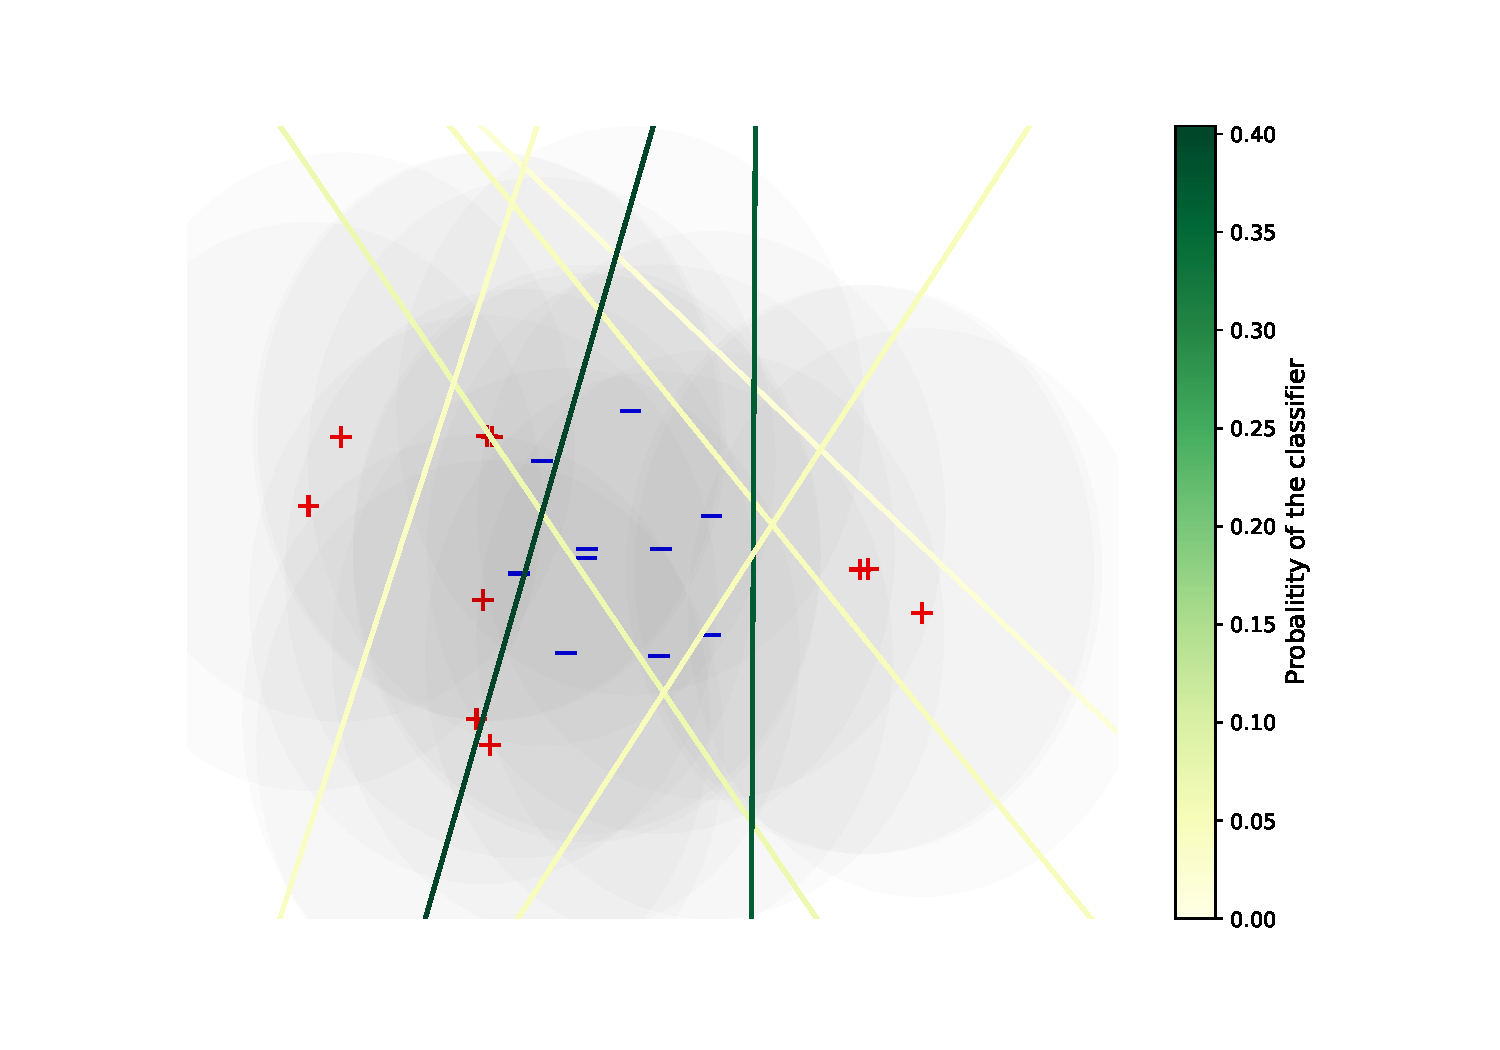
\includegraphics[width=0.32\textwidth]{Images/illustration.pdf}  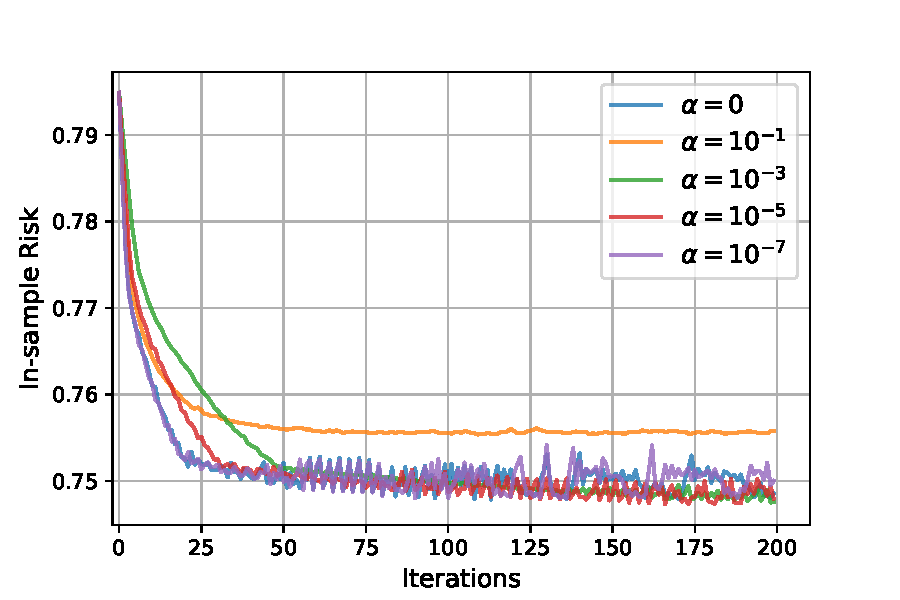
\includegraphics[width=0.32\textwidth]{Images/convergence_toy.pdf}     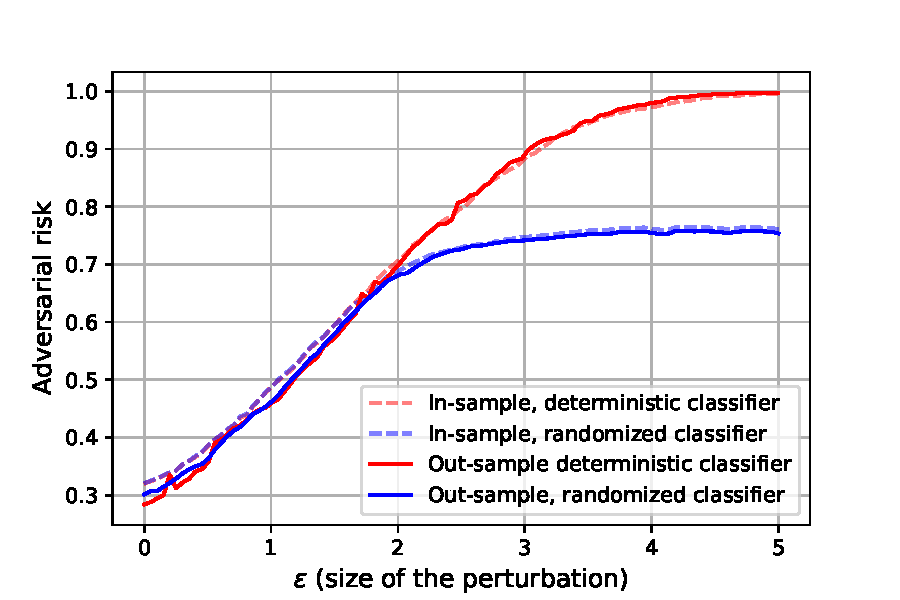
\includegraphics[width=0.32\textwidth]{Images/risk_toy.pdf}
    \caption{On left, $40$ data samples with their set of possible attacks represented in shadow and the optimal randomized classifier, with a color gradient representing the probability of the classifier. \textcolor{black}{In the middle}, convergence of the oracle ($\alpha=0$) and regularized algorithm for different values of regularization parameters. On right, in-sample and out-sample risk for randomized and deterministic minimum risk in function of the perturbation size $\varepsilon$. In the latter case, the randomized classifier is optimized with oracle Algorithm~\ref{algo:duchi}.}
    \label{fig:toy_example}
\end{figure*}


\textbf{An Entropic Relaxation.} Using the results from Section~\ref{sec:entropic-reg}, adding an entropic term to the objective allows to have a simple reformulation of the problem, as follows:
\begin{align*}
  \inf_{\bm{\lambda}\in \Delta_l}\sum_{i=1}^\numsamples  \frac{\varepsilon_i}{\numsamples}\log\left( \frac{1}{m_i}\sum_{j=1}^{m_i}\exp\left(\frac{\sum_{k=1}^l \lambda_k\loss(\theta_k,u_j^{(i)})}{\varepsilon_i}\right)\right)
\end{align*}
Note that in $\bm{\lambda}$, the objective is convex and smooth. One can  apply the accelerated PGD~\citep{beck2009fast,tseng2008accelerated} which enjoys an optimal convergence rate for first order methods of $\mathcal{O}(T^{-2})$ for $T$ iterations.

\textbf{A First Oracle Algorithm.} Indepedently from  the entropic regularization,we present an oracle-based algorithm inspired from~\citep{sinha2017certifying} and the convergence of projected sub-gradient methods~\citep{boyd2003subgradient}. The computation of the inner supremum problem is usually NP-hard. Let us justify it on a mixture of linear classifiers in binary classification: $f_{\theta_k,b_k}(x) = \langle \theta,x\rangle+b_k$ for $k\in [L]$ and $\bm{\lambda}=\mathbf{1}_L/L$. Let us consider the $\ell_2$ norm and $x=0$ and $y=1$. Then the problem of attacking $x$ is the following:
\begin{align*}
    \sup_{\tau,~\lVert \tau\rVert\leq\varepsilon} \frac{1}{L}\sum_{k=1}^L\mathbf{1}_{\langle \theta_k,x+\tau\rangle+b_k\leq0}
\end{align*}
This problem is equivalent to a linear binary classification problem on $\tau$, which is known to be NP-hard. Assuming the existence of a $\delta$-approximate oracle to this supremum, we algorithm is presented in Algorithm~\ref{algo:duchi}. We get the following guarantee for this algorithm. %See proof in Appendix~\ref{prv:algo-oracle}.
\begin{prop}
\label{prop:algo-oracle}
% Let $\PP\in\mathcal{M}^1_+(\mathcal{X}\times\mathcal{Y})$.
Let $\loss:\Theta\times(\mathcal{X}\times\mathcal{Y})\to [0,\infty)$ satisfying Assumption~\ref{ass:loss}. Then, Algorithm~\ref{algo:duchi} satisfies:  
\begin{align*}
    \min_{t\in[T]} \widehat{\mathcal{R}}_{adv}^{\varepsilon}(\bm{\lambda}_t)-\widehat{\mathcal{R}}_{adv}^{\varepsilon,*}\leq2\delta+\textcolor{black}{ \frac{2M\sqrt{l}}{\sqrt{T}}}
    % \delta\sqrt{K}+ \frac{M\sum_{t=1}^T \eta_t^2+\rVert\lambda_0-\lambda^*\lVert^2}{\sum_{t=1}^T\eta_t}
\end{align*}
% In particular for $\eta_t =\frac{\eta}{t^{1/2}}$, we get: $\min_{t\in[T]}\risk^\varepsilon(\lambda_t)-\risk^\varepsilon(\lambda^*)\in O\left(\delta+\frac{\log T}{\sqrt{T}}\right)$
\end{prop}

\begin{proof}
Thanks to Danskin theorem, if $\QQ^*$ is a best response to $\bm{\lambda}$, then $$\bm{g}^*:=\left(\mathbb{E}_{\QQ^*}\left[\loss(\theta_1,(x,y))\right],\dots,\mathbb{E}_{\QQ^*}\left[\loss(\theta_l,(x,y))\right]\right)^T$$ is a subgradient of $\bm{\lambda}\to \risk^\varepsilon(\bm{\lambda})$. Let $\eta\geq 0$ be the learning rate. Then we have for all $t\geq 1$:
\begin{align*}
\lVert \bm{\lambda}_t-\bm{\lambda}^*\rVert^2&\leq \lVert \bm{\lambda}_{t-1}-\eta \bm{g}_t-\bm{\lambda}^*\rVert^2\\
&=\lVert \bm{\lambda}_{t-1}-\bm{\lambda}^*\rVert^2-2\eta \langle\bm{g}_t, \bm{\lambda}_{t-1}-\bm{\lambda}^*\rangle+ \eta^2\lVert \bm{g}_t\rVert^2\\
&\leq \lVert \bm{\lambda}_{t-1}-\bm{\lambda}^*\rVert^2-2\eta \langle\bm{g}^*_t, \bm{\lambda}_{t-1}-\bm{\lambda}^*\rangle+2\eta\langle\bm{g}^*_t-\bm{g}_t, \bm{\lambda}_{t-1}-\bm{\lambda}^*\rangle+\eta^2 M^2 l\\
&\leq \lVert \bm{\lambda}_{t-1}-\bm{\lambda}^*\rVert^2-2\eta\left(\risk^\varepsilon(\bm{\lambda}_t)-\risk^\varepsilon(\bm{\lambda}^*)\right) +4\eta\delta+\eta^2  M^2 l%\lVert \bm{\lambda}_{t-1}-\bm{\lambda}^*\rVert_1
\end{align*}
We then deduce by summing:
\begin{align*}
   2\eta \sum_{t=1}^T \risk^\varepsilon(\bm{\lambda}_t)-\risk^\varepsilon(\bm{\lambda}^*) \leq 4\delta\eta T +\lVert \bm{\lambda}_{0}-\bm{\lambda}^*\rVert^2+\eta^2 M^2 lT
\end{align*}
Then we have:
\begin{align*}
    \min_{t\in[T]}\risk^\varepsilon(\bm{\lambda}_t)-\risk^\varepsilon(\bm{\lambda}^*)\leq 2\delta+\frac{4}{\eta T}+M^2l\eta
\end{align*}
The left-hand term is minimal for $\eta=\frac{2}{M\sqrt{lT}}$, and for this value:
\begin{align*}
    \min_{t\in[T]}\risk^\varepsilon(\bm{\lambda}_t)-\risk^\varepsilon(\bm{\lambda}^*)\leq 2\delta+\frac{2M\sqrt{l}}{\sqrt{T}}
\end{align*}
\end{proof}. 

The main drawback of the above algorithm is that one needs to have access to an oracle to guarantee the convergence of the proposed algorithm whereas its regularized version in order to approximate the solution and propose a simple algorithm to solve it.

 %In practice, we can change the distribution of sampling, to be more likely to find adversaries. 
% \begin{rmq}
% In general, one can use the exact same tools to obtain a proxy of the general DRO problem. Indeed thanks to~\citep{blanchet2019quantifying}, the dual can be approximated by adding an entropic term to the objective which leads to. We end-up with a minimization problem of a convex objective over the set of distribution. 
% \end{rmq}

\subsection{A General Heuristic Algorithm}

So far, our algorithms are not easily practicable in the case of deep learning. Adversarial examples are known to be easily transferrable from one model to another~\citep{tramer2017space,papernot2016transferability}. So we aim at learning diverse models. To this end, and support our theoretical claims, we propose an heuristic algorithm (see Algorithm~\ref{algo:heuristic}) to train a robust mixture of $l$ classifiers.   We alternatively train these classifiers with adversarial examples against the current mixture and update the probabilities of the mixture according to the algorithms we proposed in Section~\ref{sec:proposed-algo}. 


\begin{algorithm}[h!]
\SetAlgoLined
$l$: number of models, $T$: number of iterations,\\
$T_\theta$: number of updates for the models $\bm{\theta}$,\\
$T_\lambda$: number of updates for the mixture $\bm{\lambda}$,\\ $\bm{\lambda}_0=(\lambda_0^1,\dots\lambda_0^l),~\bm{\theta}_0=(\theta_0^1,\dots\theta_0^l)$\\
 \For{$t=1,\dots,T$}{
 Let $B_t$ be a batch of data.\\
\eIf{$t \mod (T_\theta l+1)\neq 0$}{
$k$ sampled uniformly in $\{1,\dots,l\}$\\
$\Tilde{B}_t\leftarrow$ Attack of images in $B_t$ for the  model $(\bm{\lambda}_t,\bm{\theta}_t)$\\
$\theta^t_k\leftarrow$ Update $\theta^{t-1}_k$ with $\Tilde{B}_t$ for fixed $\bm{\lambda}_t$ with a SGD step}{
$\bm{\lambda}_t\leftarrow$Update $\bm{\lambda}_{t-1}$ on $B_t$ for fixed $\bm{\theta}_t$
with oracle-based or regularized algorithm with $T_\lambda$ iterations.
}
  }
 \caption{Adversarial Training for Mixtures}
 
 \label{algo:heuristic}
\end{algorithm}


\section{Experiments}

\subsection{Synthetic Dataset}


To illustrate our theoretical findings, we start by testing our learning algorithm on the following synthetic two-dimensional problem. Let us consider the distribution $\PP$ defined as  $\PP\left(Y =\pm 1\right)=1/2$, $\PP\left(X\mid Y=-1\right) = \mathcal{N}(0,I_2)$ and $\PP\left(X \mid Y=1\right) = \frac12\left[\mathcal{N}((-3,0),I_2)+\mathcal{N}((3,0),I_2) \right]$.
% \begin{align*}
%   \left\{
%     \begin{array}{ll}
%   \\
%         \PP\left(X\mid Y=-1\right) = \mathcal{N}(0,I_2) \\
%         \PP\left(X \mid Y=1\right) = \frac12\left[\mathcal{N}((-3,0),I_2)+\mathcal{N}((3,0),I_2) \right].
%     \end{array}
% \right. 
% \end{align*}
We sample $1000$ training points from this distribution and randomly generate $10$ linear classifiers that achieves a standard training risk lower than $0.4$. To simulate an adversary with budget $\varepsilon$ in $\ell_2$ norm, we proceed as follows. For every sample $(x,y)\sim \PP$ we generate $1000$ points uniformly at random in the ball of radius $\varepsilon$ and select the one maximizing the risk for the $0/1$ loss. Figure~\ref{fig:toy_example} (left) illustrates the type of mixture we get after convergence of our algorithms. Note that in this toy problem, we are likely to find the optimal adversary with this sampling strategy if we sample enough attack points. 
% \begin{figure}[ht]
%     \centering
%     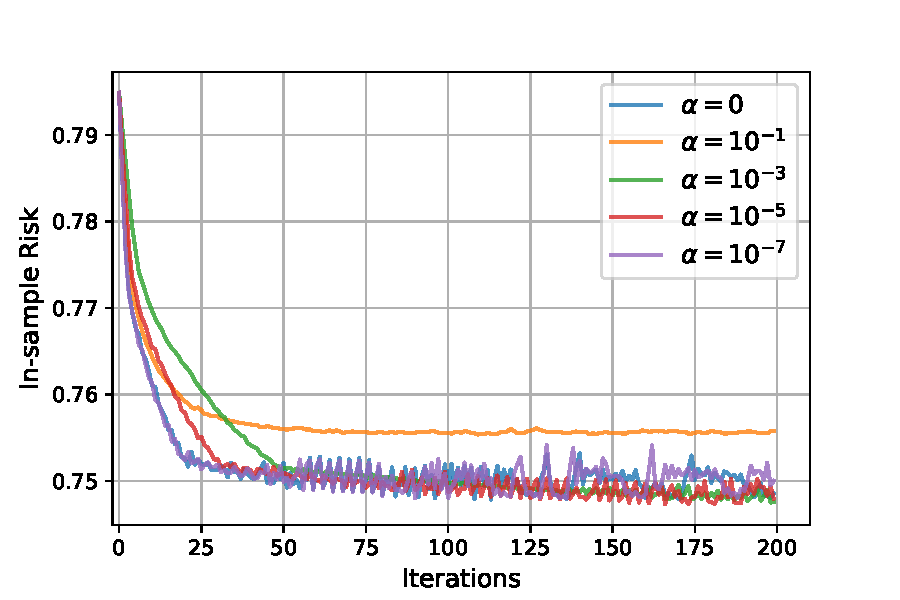
\includegraphics[width=0.46\textwidth]{Images/convergence_toy.pdf}
%     \caption{Caption}
%     \label{fig:toy_example_cvgence}
% \end{figure}
\begin{figure*}[!ht]
\begin{center}

\textbf{Adversarial Training, CIFAR-10 dataset results}
 \begin{small}
\begin{tabular}{c|c|ccc} 
\textbf{ Models} & \textbf{Acc. }&\textbf{$\textrm{APGD}_\textrm{CE}$}& \textbf{$\textrm{APGD}_\textrm{DLR}$} & \textbf{Rob. Acc.} \\ \hline
 1 & $81.9\%$ &	$47.6\%$ & $47.7\%$ & $45.6\%$ \\ 
 2 & $81.9\%$ & $49.0\%$ & ${49.6\%}$ & ${47.0\%}$\\ 
  3 & ${81.7\%}$& ${49.0\%}$ & $49.3\%$ & ${46.9\%}$\\
    4 & $\bm{82.6\%}$& $\bm{49.7\%}$ & $\bm{49.8}\%$ & $\bm{47.2\%}$\\

\end{tabular}
\end{small}\\
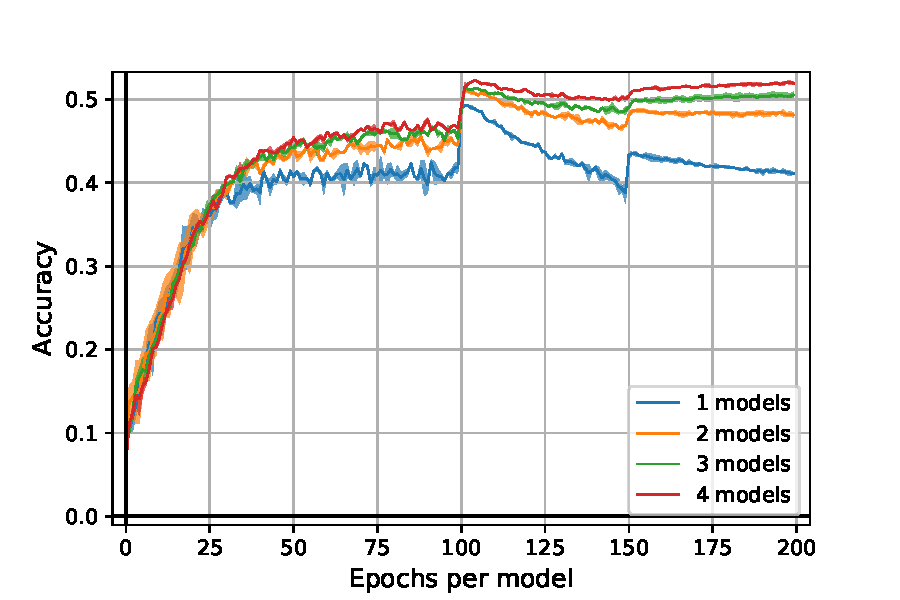
\includegraphics[width=0.35\textwidth]{Images/robust_acc_finalrun_ResNet18_1024_200_0.001.pdf}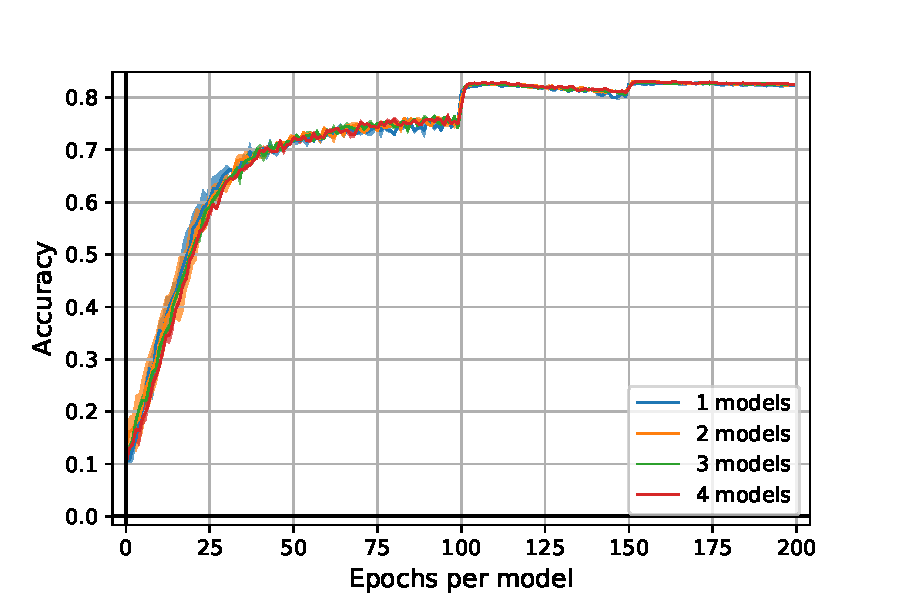
\includegraphics[width=0.35\textwidth]{Images/standard_acc_finalrun_ResNet18_1024_200_0.001.pdf} 
  

\textbf{TRADES, CIFAR-10 dataset results}

 \begin{small}
\begin{tabular}{c|c|ccc} 
\textbf{ Models} & \textbf{Acc. }&\textbf{$\textrm{APGD}_\textrm{CE}$}& \textbf{$\textrm{APGD}_\textrm{DLR}$} & \textbf{Rob. Acc.} \\ \hline
 1 &  $79.6\%$ &$50.9\%$& $48.9\%$ &$48.3\%$ \\ 
 2 & $80.3\%$& $52.3\%$ &$51.2\%$ &$50.2\%$\\ 
  3 & $80.7\%$& $52.8\%$ &$51.7\%$ &$50.7\%$\\
    4 & \bm{$80.9\%$} & \bm{$53.0\%$}& \bm{$51.8\%$}& \bm{$50.8\%$}\\

\end{tabular}
\end{small}

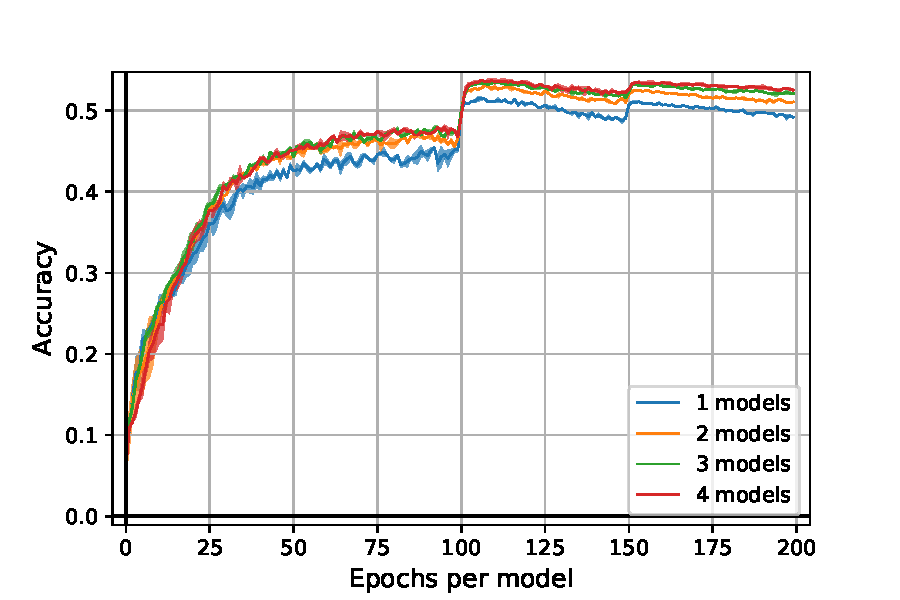
\includegraphics[width=0.35\textwidth]{Images/robust_acc_CIFAR10_final_cam_ready_bisss_ResNet18_1024_200_0.001.pdf}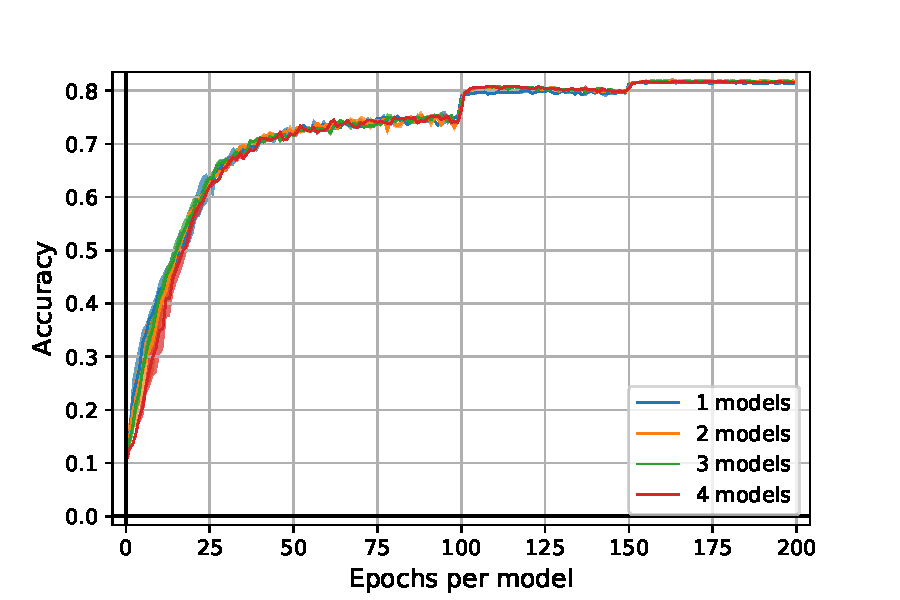
\includegraphics[width=0.35\textwidth]{Images/standard_acc_CIFAR10_final_cam_ready_bisss_ResNet18_1024_200_0.001.pdf} 
  

\textbf{Adversarial Training, CIFAR-100 dataset results}
 \begin{small}
\begin{tabular}{c|c|ccc} 
\textbf{ Models} & \textbf{Acc. }&\textbf{$\textrm{APGD}_\textrm{CE}$}& \textbf{$\textrm{APGD}_\textrm{DLR}$} & \textbf{Rob. Acc.} \\ \hline
 1 & $55.2\%$& $24.1\%$& $23.8\%$ & $22.5\%$\\ 
 2 & $55.2\%$ & $25.3\%$ &$26.1\%$ &$23.6\%$\\ 
  3 & \bm{$55.4\%$} & $25.7\%$ &$26.8\%$ &$24.2\%$\\
    4 & $55.3\%$ & \bm{$26.0\%$} & \bm{$27.5\%$}& \bm{$24.5\%$}\\

\end{tabular}
\end{small}
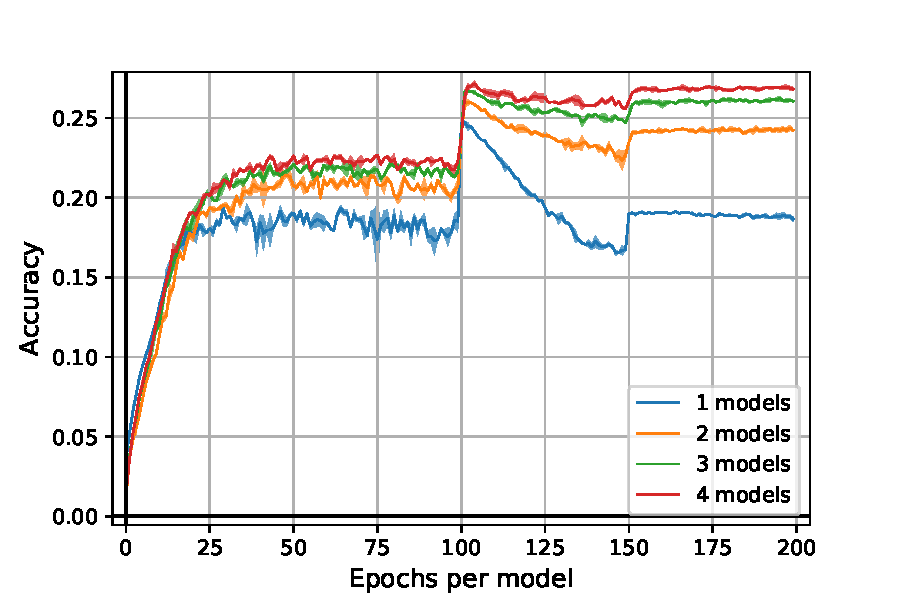
\includegraphics[width=0.35\textwidth]{Images/robust_acc_CIFAR100_finalrun_ResNet18_1024_200_0.001.pdf}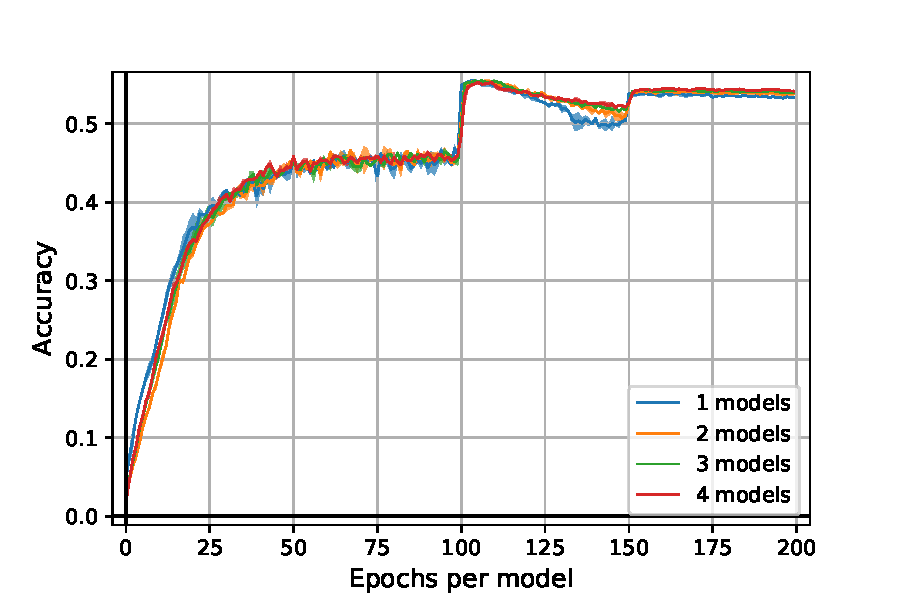
\includegraphics[width=0.35\textwidth]{Images/standard_acc_CIFAR100_finalrun_ResNet18_1024_200_0.001.pdf} 


 \caption{Upper plots: Adversarial Training, CIFAR-10 dataset results. Middle plots:  TRADES, CIFAR-10 dataset results. Bottom plots: CIFAR-100 dataset results. {On left}: Comparison of our algorithm with a standard adversarial training (one model). We reported the results for the model with the best robust accuracy obtained over two independent runs because adversarial training might be unstable. Standard and Robust accuracy (respectively in the middle and on right) on CIFAR-10 test images in function of the number of epochs per classifier with $1$ to $3$ ResNet18 models. The performed attack is PGD with $20$ iterations and $\varepsilon=8/255$.}
\label{fig:results_cifar}

\end{center}
\end{figure*}

To evaluate the convergence of our algorithms, we compute the adversarial risk of our mixture for each iteration of both the oracle and regularized algorithms. Figure~\ref{fig:toy_example} illustrates the convergence of the algorithms w.r.t the regularization parameter. We observe that the risk for both algorithms converge. Moreover, they converge towards the oracle minimizer when the regularization parameter $\alpha$ goes to $0$.

Finally, to demonstrate the improvement randomized techniques offer against deterministic defenses, we plot in Figure~\ref{fig:toy_example} (right) the minimum adversarial risk for both randomized and deterministic classifiers w.r.t. $\varepsilon$. The adversarial risk is strictly better for randomized classifier whenever the adversarial budget $\varepsilon$ is bigger than $2$. This illustration validates our analysis of Theorem~\ref{thm:duality-rand}, and motivates a in depth study of a more challenging framework, namely image classification with neural networks.

% \begin{figure}[ht]
%     \centering
%     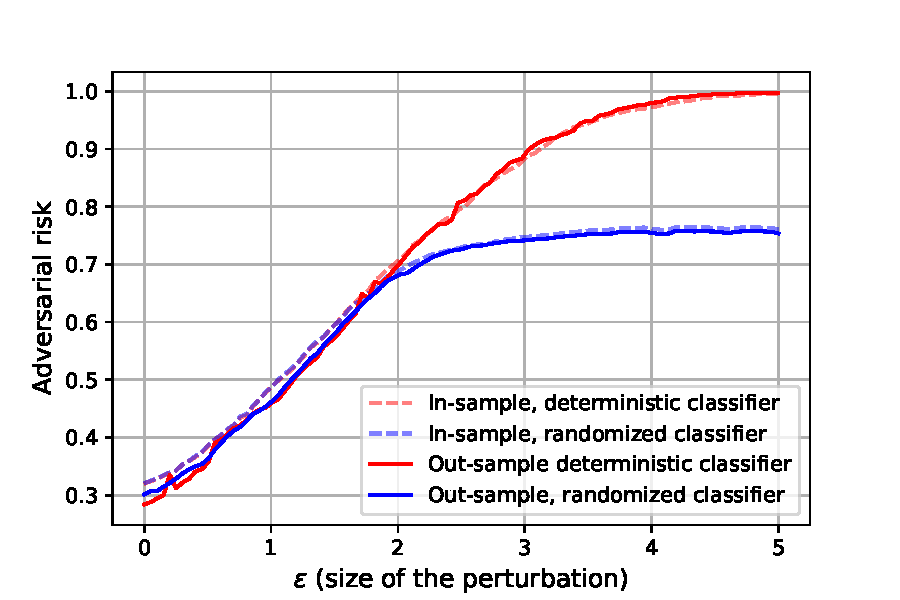
\includegraphics[width=0.46\textwidth]{Images/risk_toy.pdf}
%     \caption{Caption}
%     \label{fig:toy_example_risk}
% \end{figure}

\subsection{CIFAR Datasets}

% \begin{figure*}[!ht]
% \begin{center}

% \vskip 0.15in
%  \begin{minipage}[ht!]{0.39\textwidth}
%  \begin{scriptsize}
% \begin{tabular}{c|c|ccc} 
% \textbf{ Models} & \textbf{Acc. }&\textbf{$\textrm{APGD}_\textrm{CE}$}& \textbf{$\textrm{APGD}_\textrm{DLR}$} & \textbf{Rob. Acc.} \\ \hline
%  1 & $81.9\%$ &	$47.6\%$ & $47.7\%$ & $45.6\%$ \\ 
%  2 & $81.9\%$ & $49.0\%$ & ${49.6\%}$ & ${47.0\%}$\\ 
%   3 & ${81.7\%}$& ${49.0\%}$ & $49.3\%$ & ${46.9\%}$\\
%     4 & $\bm{82.6\%}$& $\bm{49.7\%}$ & $\bm{49.8}\%$ & $\bm{47.2\%}$\\

% \end{tabular}
% \end{scriptsize}
%   \end{minipage}\begin{minipage}[!ht]{0.61\textwidth}
% 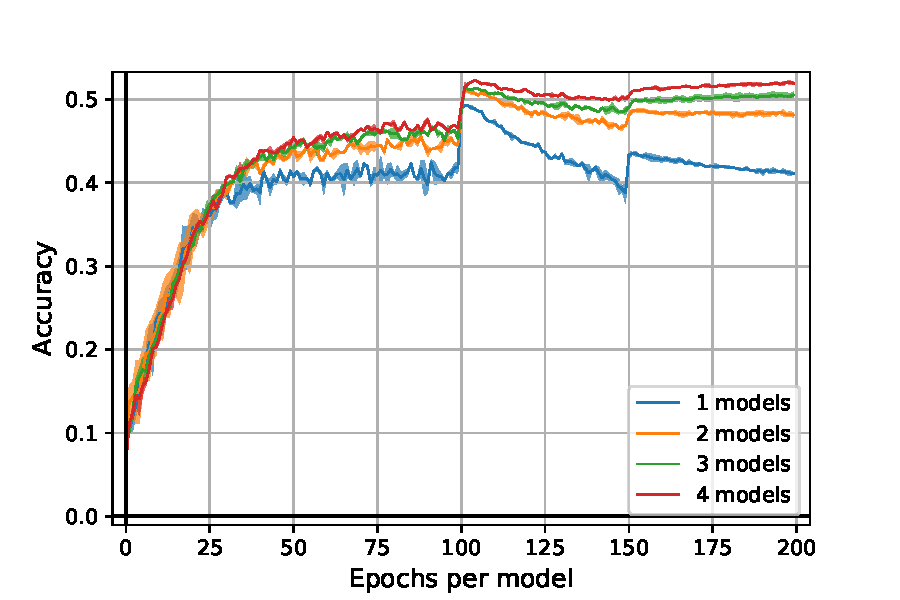
\includegraphics[width=0.49\textwidth]{Images/robust_acc_finalrun_ResNet18_1024_200_0.001.pdf}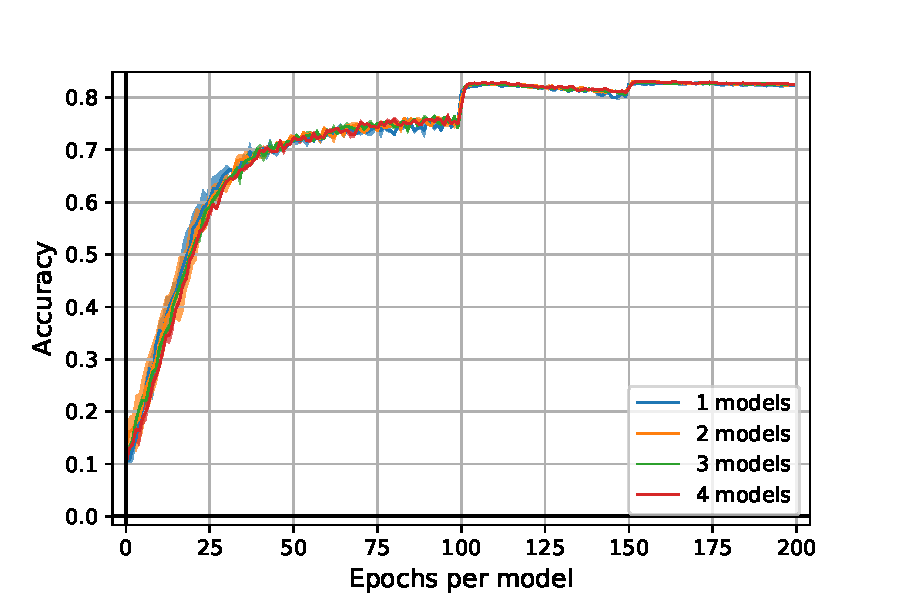
\includegraphics[width=0.49\textwidth]{Images/standard_acc_finalrun_ResNet18_1024_200_0.001.pdf} 
%   \end{minipage}
  
% Adversarial Training, CIFAR-10 dataset results

% \vskip 0.15in
%  \begin{minipage}[ht!]{0.39\textwidth}
%  \begin{scriptsize}
% \begin{tabular}{c|c|ccc} 
% \textbf{ Models} & \textbf{Acc. }&\textbf{$\textrm{APGD}_\textrm{CE}$}& \textbf{$\textrm{APGD}_\textrm{DLR}$} & \textbf{Rob. Acc.} \\ \hline
%  1 &  $79.6\%$ &$50.9\%$& $48.9\%$ &$48.3\%$ \\ 
%  2 & $80.3\%$& $52.3\%$ &$51.2\%$ &$50.2\%$\\ 
%   3 & $80.7\%$& $52.8\%$ &$51.7\%$ &$50.7\%$\\
%     4 & \bm{$80.9\%$} & \bm{$53.0\%$}& \bm{$51.8\%$}& \bm{$50.8\%$}\\

% \end{tabular}
% \end{scriptsize}
%   \end{minipage}\begin{minipage}[!ht]{0.61\textwidth}
% 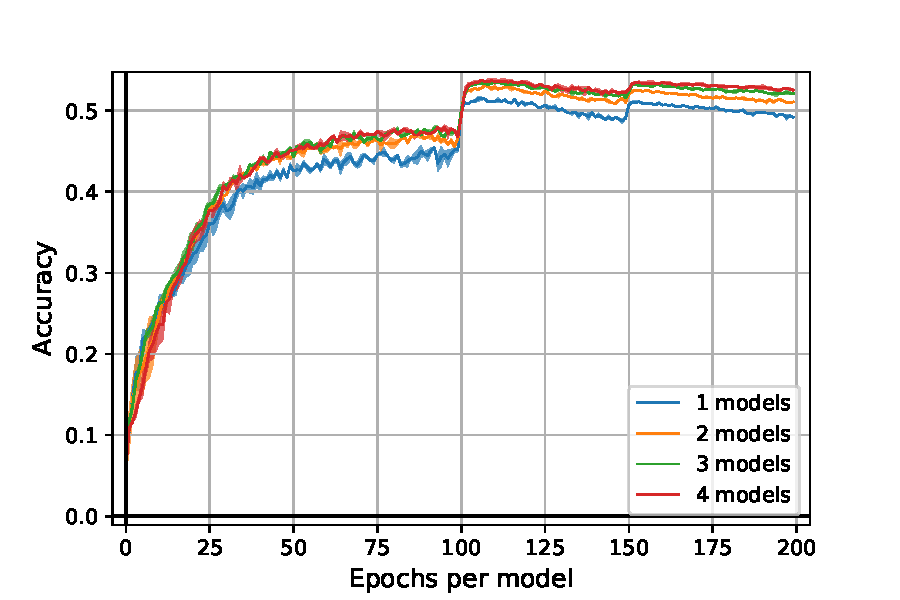
\includegraphics[width=0.49\textwidth]{Images/robust_acc_CIFAR10_final_cam_ready_bisss_ResNet18_1024_200_0.001.pdf}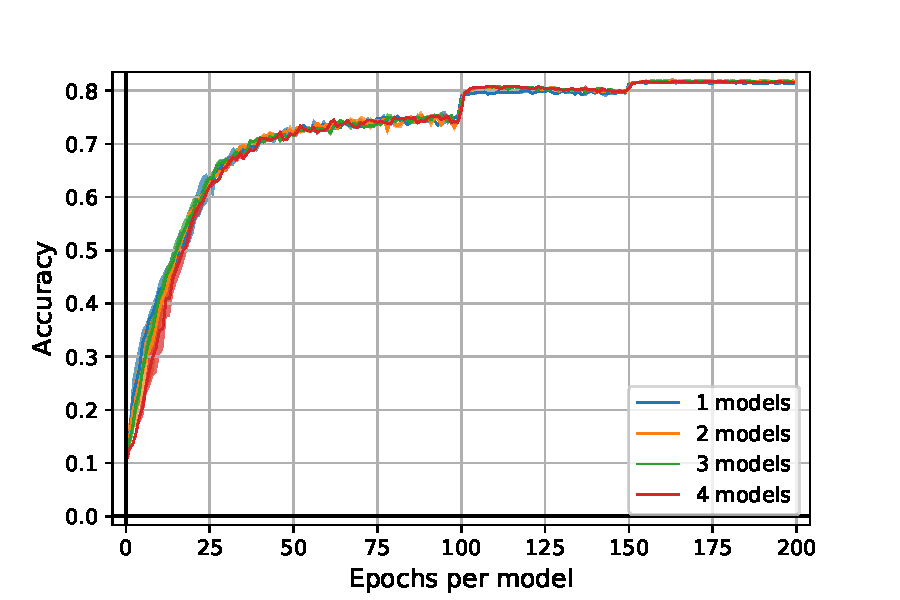
\includegraphics[width=0.49\textwidth]{Images/standard_acc_CIFAR10_final_cam_ready_bisss_ResNet18_1024_200_0.001.pdf} 
%   \end{minipage}
  
% TRADES, CIFAR-10 dataset results
% \vskip 0.15in
%  \begin{minipage}[ht!]{0.39\textwidth}
%  \begin{scriptsize}
% \begin{tabular}{c|c|ccc} 
% \textbf{ Models} & \textbf{Acc. }&\textbf{$\textrm{APGD}_\textrm{CE}$}& \textbf{$\textrm{APGD}_\textrm{DLR}$} & \textbf{Rob. Acc.} \\ \hline
%  1 & $55.2\%$& $24.1\%$& $23.8\%$ & $22.5\%$\\ 
%  2 & $55.2\%$ & $25.3\%$ &$26.1\%$ &$23.6\%$\\ 
%   3 & \bm{$55.4\%$} & $25.7\%$ &$26.8\%$ &$24.2\%$\\
%     4 & $55.3\%$ & \bm{$26.0\%$} & \bm{$27.5\%$}& \bm{$24.5\%$}\\

% \end{tabular}
% \end{scriptsize}
%   \end{minipage}\begin{minipage}[!ht]{0.61\textwidth}
% 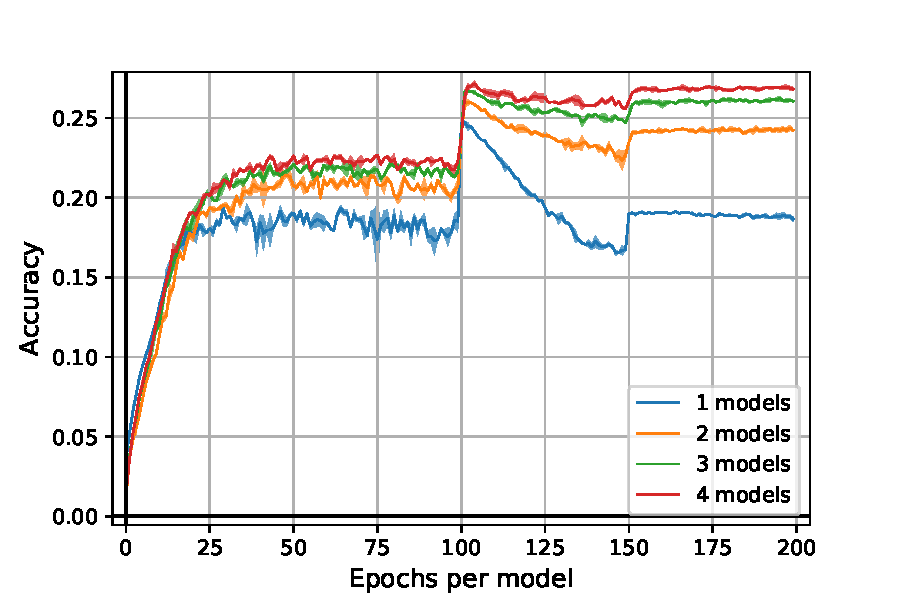
\includegraphics[width=0.49\textwidth]{Images/robust_acc_CIFAR100_finalrun_ResNet18_1024_200_0.001.pdf}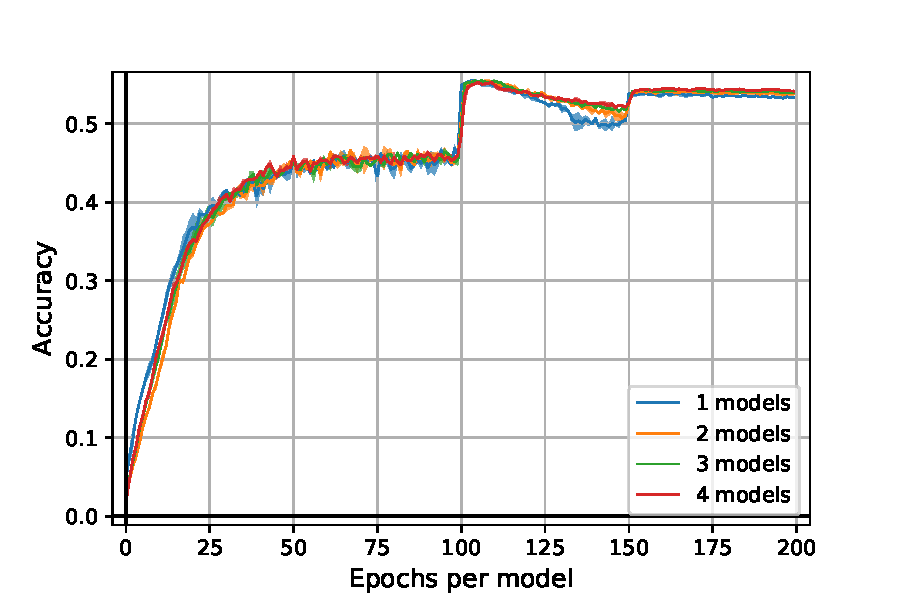
\includegraphics[width=0.49\textwidth]{Images/standard_acc_CIFAR100_finalrun_ResNet18_1024_200_0.001.pdf} 
%   \end{minipage}
%   Adversarial Training, CIFAR-100 dataset results

%  \caption{Upper plots: Adversarial Training, CIFAR-10 dataset results. Middle plots:  TRADES, CIFAR-10 dataset results. Bottom plots: CIFAR-100 dataset results. {On left}: Comparison of our algorithm with a standard adversarial training (one model). We reported the results for the model with the best robust accuracy obtained over two independent runs because adversarial training might be unstable. Standard and Robust accuracy (respectively in the middle and on right) on CIFAR-10 test images in function of the number of epochs per classifier with $1$ to $3$ ResNet18 models. The performed attack is PGD with $20$ iterations and $\varepsilon=8/255$.}
% \label{fig:results_cifar}

% \end{center}
% \end{figure*}

% Adversarial examples are known to be easily transferrable from one model to another~\cite{tramer2017space}. To counter this and support our theoretical claims, we propose an heuristic algorithm (see Algorithm~\ref{algo:heuristic}) to train a robust mixture of $L$ classifiers. We alternatively train these classifiers with adversarial examples against the current mixture and update the probabilities of the mixture according to the algorithms we proposed in Section~\ref{sec:proposed-algo}. More details on the heuristic algorithm are available in Appendix~\ref{sec:additional-xp}. 
% \begin{algorithm}[h!]
% \small
% \SetAlgoLined
% $L$: number of models, $T$: number of iterations,\\
% $T_\theta$: number of updates for the models $\bm{\theta}$,\\
% $T_\lambda$: number of updates for the mixture $\bm{\lambda}$,\\ $\bm{\lambda}_0=(\lambda_0^1,\dots\lambda_0^L),~\bm{\theta}_0=(\theta_0^1,\dots\theta_0^L)$\\
%  \For{$t=1,\dots,T$}{
%  Let $B_t$ be a batch of data.\\
% \eIf{$t \mod (T_\theta L+1)\neq 0$}{
% $k$ sampled uniformly in $\{1,\dots,L\}$\\
% $\Tilde{B}_t\leftarrow$ Attack of images in $B_t$ for the  model $(\bm{\lambda}_t,\bm{\theta}_t)$\\
% $\theta^t_k\leftarrow$ Update $\theta^{t-1}_k$ with $\Tilde{B}_t$ for fixed $\bm{\lambda}_t$ with a SGD step}{
% $\bm{\lambda}_t\leftarrow$Update $\bm{\lambda}_{t-1}$ on $B_t$ for fixed $\bm{\theta}_t$
% with oracle or regularized algorithm with $T_\lambda$ iterations.
% }
%   }
%  \caption{Adversarial Training for Mixtures}
 
%  \label{algo:heuristic}
% \end{algorithm}

\paragraph{Experimental Setup.} We now implement our heuristic algorithm (Alg.~\ref{algo:heuristic}) on CIFAR-10 and CIFAR-100 datasets for both Adversarial Traning~\citep{madry2017towards} and TRADES~\citep{zhang2019theoretically} loss. To evaluate the performance of Algorithm~\ref{algo:heuristic}, we trained from $1$ to $4$ ResNet18~\citep{He_2016_CVPR} models on $200$ epochs per model\footnote{$L\times200$ epochs in total, where $L$ is the number of models.}. We study the robustness with regards to $\ell_\infty$ norm and fixed adversarial budget $\varepsilon=8/255$. The attack we used in the inner maximization of the training is an adapted (adaptative) version of PGD for mixtures of classifiers with $10$ steps. Note that for one single model, Algorithm~\ref{algo:heuristic} exactly corresponds to adversarial training~\citep{madry2017towards} or TRADES. For each of our setups, we made two independent runs and select the  best one. The training time of our algorithm is around four times longer than a standard Adversarial Training (with PGD 10 iter.) with two models, eight times with three models and twelve times with four models. We trained our models with a batch of size  $1024$ on $8$ Nvidia V100 GPUs. 

\paragraph{Optimizer.} For each of our models, The optimizer we used in all our implementations is SGD with learning rate set to $0.4$ at epoch $0$ and is divided by $10$ at half training then by $10$ at the three quarters of training. The momentum is set to $0.9$ and the weight decay to $5\times10^{-4}$. The batch size is set to $1024$. 
\paragraph{Adaptation of Attacks.} Since our classifier is randomized, we need to adapt the attack accordingly. To do so we used the expected loss:
\begin{align*}
\Tilde{\loss}\left((\bm{\lambda},\bm{\theta}),(x,y)\right) = \sum_{k=1}^L \lambda_k \loss(\theta_k,(x,y))
\end{align*}
to compute the gradient in the attacks, regardless the loss (DLR or cross-entropy). For the inner maximization at training time, we used a PGD attack on the cross-entropy loss with $\varepsilon=0.03$. For the final evaluation, we used the untargeted $DLR$ attack with default parameters.
\paragraph{Regularization in Practice.} The entropic regularization in higher dimensional setting need to be adapted to be more likely to find adversaries. To do so, we computed PGD attacks with only $3$ iterations with $5$ different restarts instead of sampling uniformly $5$ points  in the $\ell_\infty$-ball. In our experiments in the main paper, we use a regularization parameter $\alpha=0.001$. The learning rate for the minimization on $\bm{\lambda}$ is always fixed to $0.001$. 
\paragraph{Alternate Minimization Parameters.} Algorithm~\ref{algo:heuristic} implies an alternate minimization algorithm. We set the number of updates of $\bm{\theta}$ to $T_\theta = 50$ and, the update of $\bm{\lambda}$ to $T_\lambda = 25$. 

\subsection{Effect of the Regularization}
In this subsection, we experimentally investigate the effect of the regularization. In Figure~\ref{fig:xp-regularization}, we notice, that the regularization has the effect of stabilizing, reducing the variance and improving the level of the robust accuracy for adversarial training for mixtures (Algorithm~\ref{algo:heuristic}). The standard accuracy curves are very similar in both cases.



\paragraph{Evaluation Protocol.} At each epoch, we evaluate the current mixture on test data against PGD attack  with $20$ iterations. To select our model and avoid overfitting~\citep{rice2020overfitting}, we kept the most robust against this PGD attack.
To make a final evaluation of our mixture of models, we used an adapted version of $\textrm{AutoPGD}$ untargeted attacks~\citep{croce2020reliable} for randomized classifiers with both Cross-Entropy (CE) and Difference of Logits Ratio (DLR) loss. For both attacks, we made $100$ iterations and $5$ restarts.

\paragraph{Results.} The results are presented in Figure~\ref{fig:results_cifar}. We remark our algorithm outperforms a standard adversarial training in all the cases by more $1\%$ on CIFAR-10 and CIFAR-100, without additional loss of standard accuracy as it is attested by the left figures. On TRADES, the gain is even more important by more than $2\%$ in robust accuracy. Moreover, it seems our algorithm, by adding more and more models, reduces the overfitting of adversarial training. It also appears that robustness increases as the number of models increases. So far, experiments are computationally very costful and it is difficult to raise precise conclusions. Further, hyperparameter tuning ~\citep{gowal2020uncovering} such as architecture, unlabeled data~\citep{carmon2019unlabeled} or activation function may still increase the results.





% \begin{figure*}[!ht]
% \begin{center}


% \label{table:results}
% \vskip 0.15in
%  \begin{minipage}[!ht]{0.39\textwidth}
%  \begin{scriptsize}
% \begin{tabular}{c|c|ccc} 
% \textbf{ Models} & \textbf{Acc. }&\textbf{$\textrm{APGD}_\textrm{CE}$}& \textbf{$\textrm{APGD}_\textrm{DLR}$} & \textbf{Rob. Acc.} \\ \hline
%  1 & $81.9\%$ &	$47.6\%$ & $47.7\%$ & $45.6\%$ \\ 
%  2 & $81.9\%$ & $49.0\%$ & ${49.6\%}$ & ${47.0\%}$\\ 
%   3 & ${81.7\%}$& ${49.0\%}$ & $49.3\%$ & ${46.9\%}$\\
%     4 & $\bm{82.6\%}$& $\bm{49.7\%}$ & $\bm{49.8}\%$ & $\bm{47.2\%}$\\

% \end{tabular}
% \end{scriptsize}
%   \end{minipage}\begin{minipage}[!ht]{0.61\textwidth}
% 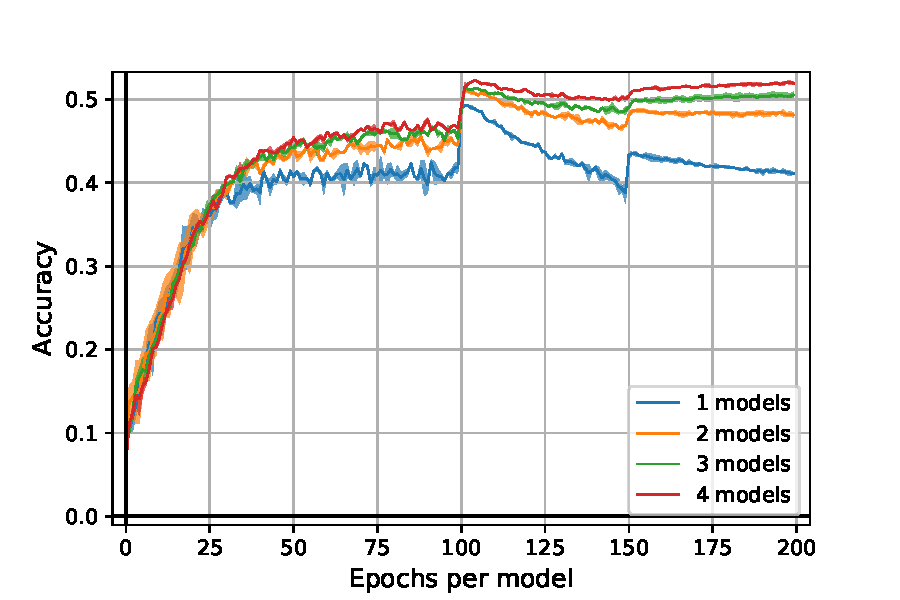
\includegraphics[width=0.49\textwidth]{Images/robust_acc_finalrun_ResNet18_1024_200_0.001.pdf}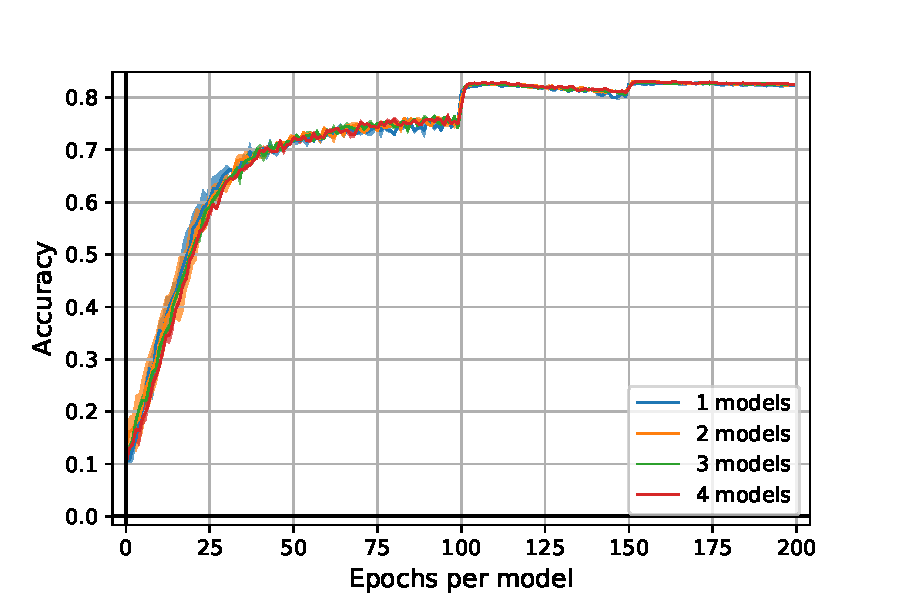
\includegraphics[width=0.49\textwidth]{Images/standard_acc_finalrun_ResNet18_1024_200_0.001.pdf} 
%   \end{minipage}
  
% \caption{On left: Comparison of our algorithm with a standard adversarial training (one model). We reported the results for the model with the best robust accuracy obtained over two independent runs because adversarial training might be unstable. Standard and Robust accuracy ( respectively in the center and on left) on CIFAR-10 test images in function of the number of epochs per classifier with $1$ to $3$ ResNet18 models. The performed attack is PGD with $20$ iterations and $\varepsilon=8/255$.}
% \label{fig:results_cifar}
% \end{center}
% \end{figure*}











% \begin{figure}[!ht]
% 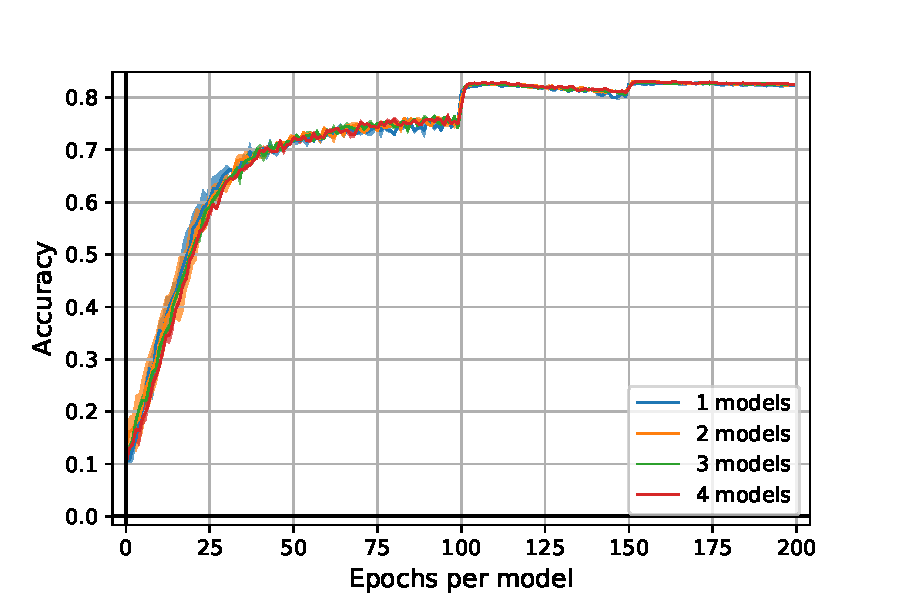
\includegraphics[width=0.46\textwidth]{Images/standard_acc_finalrun_ResNet18_1024_200_0.001.pdf}    \caption{Standard accuracy on CIFAR-10 test images in function of the number of epochs per classifier with $1$ to $3$ ResNet18 models.}
%     \label{fig:plot_standard_acc}
% \end{figure}

% \begin{figure}[!ht]
% 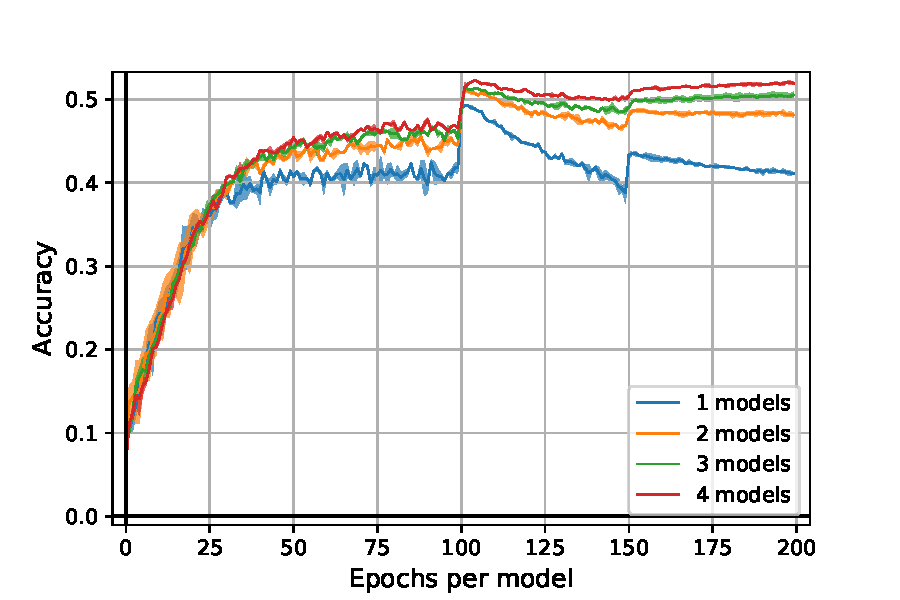
\includegraphics[width=0.46\textwidth]{Images/robust_acc_finalrun_ResNet18_1024_200_0.001.pdf}    \caption{Robust accuracy on CIFAR-10 test images in function of the number of epochs per classifier with $1$ to $3$ ResNet18 models. The attack performed is PGD with $20$ iterations and $\varepsilon=8/255$.}
%     \label{fig:plot_robust_acc}
% \end{figure}



% mettre ca au propre mais les resultats sont la!!

% setup: ResNet18 ou WRN28x10

% Details in supmat: loss +lr + format of training etc

% In supmat: 
% \begin{enumerate}
%     \item details HP (attack + training)
%     \item details runtime
%     \item additional results (with other attacks maybe + other archis...)
    
    
% \end{enumerate}
% Epochs 100

\chapter{Consistency Study of Adversarial loss}
\label{chap:calibration}

\minitoc
\textbf{Disclaimer: This section is still an unachieved work}

In this section we assume a binary classification task, i.e. an output space $\mathcal{Y}=\{-1,+1\}$. W extend the notion of loss functions to general cost functions.  A cost function is a function $\loss:\mathcal{X}\times\mathcal{Y}\times \mathcal{F}(\mathcal{X})\to \mathbb{R}$ such that $\loss(\cdot,\cdot,f)$ is universally measurable for all $f\in\mathcal{F}(\mathcal{X})$. We will denote $\mathcal{R}_{\loss}$ the risk associated with a loss $\loss$. 


\section{Loss Consistency in Classification}

\subsection{Consistency in Standard Classification}
In a standard classification setting,  given $(x,y)$, we recall  the classification loss is defined as:
\begin{align*}
    \loss_{0/1}(x,y,f) = \mathbf{1}_{y\sign(f(x))\leq 0}
\end{align*}
In the literature the notion of consistency with regards to the $0/1$ loss is defined as follows.
\begin{definition}[Classification Consistency]
A cost function $\loss$ is said to be consistent with respect to $0/1$ loss for a a probability distribution $\PP\in\mathcal{M}_1^+(\mathcal{X}\times\mathcal{Y})$ if and only if for all sequences $(f_n)_n $ of measurable functions:
\begin{align}
    \mathcal{R}_{\loss}(f_n)\to \mathcal{R}_{\loss}^\star\implies\mathcal{R}_{0/1}(f_n)\to \mathcal{R}_{0/1}^\star
\end{align}
\end{definition}


\paragraph{Standard results in classification.} Previous literature have focused, in standard classification, on margin losses, and it is defined as follows.

\begin{definition}[Margin loss] We say a loss $\loss$ is a margin loss if there exists a measurable function $\phi:\mathbb{R}\to\mathbb{R}_+$, such that for all $x\in\mathcal{X}$, $y\in\mathcal{Y}$, $f:\mathcal{X}\to\mathbb{R}$ a measurable function,
$$\loss(x,y,f)=\phi(yf(x))$$
\end{definition}
Without loss of generality, we will denote $\mathcal{R}_\phi$ the risk associated with a margin loss. Standard classification consistency highly relies on the fact that given a loss, the minimization can be made pointwisely, independently from the considered distribution $\PP$. The notion of consistency exactly matches with the notion of calibration, defined as follows:
\begin{definition}[Classification Calibration] A margin loss $\phi$ is said to be classification-calibrated if for all $\eta\in[0,1]$, $\eta\neq \frac12$:
\begin{align*}
    H(\eta)>H^-(\eta)
\end{align*}
where $H(\eta):=\inf_{\alpha\in\RR}C_\eta(\alpha)$,  $H^-(\eta) = \inf_{\alpha,~\alpha(2\eta-1)\leq0}C_\eta(\alpha)$ and $C_\eta(\alpha):=\eta\phi(\alpha)+(1-\eta)\phi(-\alpha)$.
\end{definition}

\cite{bartlett2006convexity} and \cite{steinwart2007compare} show that consistency and calibration are equivalent notions in standard classification.

\begin{thm} In standard calibration, a margin loss $\phi$ is consistent with regards to classification loss if and only if $\phi$ is classification calibrated. 
\end{thm}

In particular, one can state the following results on convex margin losses.
\begin{thm} Let $\phi$ be a convex margin differentiable in $0$. $\phi$ is consistent with regards to  classification loss if and only if $\phi'(0)<0$.
\end{thm}
\paragraph{What is the good 0/1 loss?}
In this paragraph, we precise why this $0/1$ loss is used in consistency/calibration study. Let $f:\mathcal{X}\to\mathbb{R}$ be a measurable function. In the literature,  we generally find three ways for defining the $0/1$ loss:
\begin{itemize}
    \item $\loss_{\leq}(x,y,f)=\mathbf{1}_{yf(x)\leq 0}$, the loss that penalizes indecision.
    \item $\loss_{<}(x,y,f)=\mathbf{1}_{yf(x)< 0}$, the loss that encourages indecision.
    \item $\loss_{0/1}(x,y,f)=\mathbf{1}_{y\text{sign}(f(x))\leq 0}$, with a sign convention ($sign(0) = 1$ for instance).
\end{itemize}

The original results from~\citep{bartlett2006convexity,steinwart2007compare} tackles the problem of the consistency with respect to the latter one. We can even remark that usual consistency results stated in the two previous papers are false for the two first losses, as shown in the following simple counterexample.

\begin{counterexample*}
Let $\PP$ defined as follows: $\PP(Y=-1)=\PP(Y=1)=\frac12$, and $\PP(X=0\mid Y)=1$. Let $\phi:\mathbb{R}\to\mathbb{R}$ be a margin  loss. The $\phi$-risk minimization problem writes $\inf_{\alpha} \frac{1}{2} (\phi(\alpha)+\phi(-\alpha))$. For a convex margin loss $\phi$ the optimum is attained in $\alpha=0$. 
\begin{enumerate}
    \item $f_n:x\mapsto 0$ is a minimizing sequence for the $\phi$-risk. However $R_{\loss_{\leq}}(f_n)=1$ for all $n$ and $R_{\loss_{\leq}}^*=\frac{1}{2}$. Then we deduce that no convex margin based loss can be calibrated for $\loss_{\leq}$.
    \item $f_n:x\mapsto \frac{1}{n}$ is a minimizing sequence for the $\phi$-risk. However $R_{\loss_{<}}(f_n)=1/2$ for all $n$ and $R_{\loss_{<}}^*=0$. Then we deduce that no convex margin based loss can be calibrated for $\loss_{<}$.
\end{enumerate}

\end{counterexample*}



\subsection{Consistency in adversarial setting}


Consistency in standard classification is studied with respect to the cost $\loss_{0/1}(x,y,f)=\mathbf{1}_{y\text{sign}(f(x))\leq 0}$. In the adversarial setting, the natural loss to consider then is  $$\loss_{0/1,\varepsilon}(x,y,f)=\sup_{x'\in B_\varepsilon(x)}\mathbf{1}_{y\text{sign}(f(x'))\leq 0}$$ 
with a sign convention (e.g. $sign(0)=1$). Otherwise, when $\varepsilon=0$, the consistency results would be wrong as stated in the previous counterexample. Previous works~\citep{pmlr-v125-bao20a,awasthi2021calibration,awasthi2021finer} focused on the loss $\sup_{x'\in B_\varepsilon(x)}\mathbf{1}_{yf(x')\leq 0}$ that consequently lead to misleading results because not compatible with standard classification when $\varepsilon=0$. We define the notion of consistency with regards to adversarial $0/1$ loss as follows.
\begin{definition}[Adversarial Consistency]
A cost function $\loss$ is said to be consistent with respect to $0/1$ loss for a distribution  $\PP\in\mathcal{M}_1^+(\mathcal{X}\times\mathcal{Y})$ if and only if for all sequences $(f_n)_n $ of measurable functions:
\begin{align}
    \mathcal{R}_{\loss}(f_n)\to \mathcal{R}_{\loss}^\star\implies\mathcal{R}_{0/1}^\varepsilon(f_n)\to \mathcal{R}_{0/1}^{\varepsilon,\star}
\end{align}
\end{definition}

\paragraph{Calibration in adversarial classification} One need to note that the notion of calibration in the adversarial setting is misleading.  

TODO.



Hence, one need to focus specifically on the notion of consistency in the adversarial setting. In the next section, we prove some results on adversarial consistency.

\section{Adversarial Consistency Results}

\subsection{Convex Losses are not Consistent}
Following the work on standard classification, natural candidate losses for adversarial consistency would be suprema of standardly calibrared margin losses:

$$\loss(x,y,f)=\sup_{x', d(x,x')\leq\varepsilon}\phi(yf(x))$$
including a wide range of  convex functions $\phi$. Next theorem shows the counter-intuitive result that no calibrated convex loss can define a consistent loss for adversarial classification
\begin{prop}
Let $\phi$ be a convex classification-calibrated margin loss (i.e. $\phi'(0) <0$). In $\RR$, for any $\varepsilon > 0$, there exists a distribution $\PP$ such that $x\to\sup_{x', d(x,x')\leq\varepsilon}\phi(yf(x))$ is not consistent for $\PP$ with regards to $\loss_{0/1,\varepsilon}$.
\end{prop}

\begin{proof}

Let $\epsilon$ > 0. We will construct a distribution $\mathcal{D}$ and a sequence of classifier $h_n$ so that the $\phi$-risk converges toward the optimal, while the $0-1$ loss remains constant at a non-optimal value.

\paragraph{}Let a such that $\epsilon < a < 2 \epsilon$. We define D by :
\[
\left\{ \begin{array}{ll}
\mathbb{P}(Y=1, X=0) = \frac{1}{2} & \\
\mathbb{P}(Y=-1, X=-a) = \frac{1}{4} & \\
\mathbb{P}(Y=-1, X=a) = \frac{1}{4} & \\
\mathbb{P}(X, Y) = 0 & \mbox{otherwise.} \\
\end{array} \right.
\]

Since $\phi$ is classification-calibrated, it is either non-increasing, or it has a minimum, attained on a point $u>0$. Let us consider both cases :

\paragraph{First case : $\phi$ non-increasing}

We define $Z_1 = [-\epsilon, -a + \epsilon]$ and $Z_2 = [a-\epsilon, \epsilon]$, the zones that can be attacked by two points at once.
Let us then define : 
\[
\forall x \in \mathbb{R}, h_n(x) = \left\{ \begin{array}{ll}
\frac{1}{n} & \mbox{if } x \in Z_1 \\
-1/n & \mbox{if } x \in Z_2 \\
1 & \mbox{if }x \in [-a+\epsilon, a-\epsilon] \\
-1 & \mbox{otherwise} \\
\end{array} \right.
\]

\begin{figure}
    \centering
    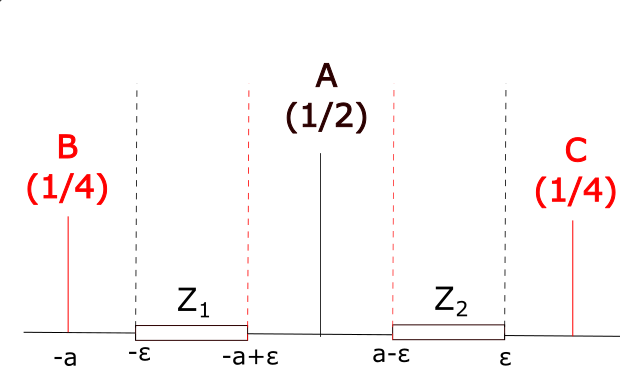
\includegraphics[scale=0.6]{sections/3_calibration/images/example.png}
    \caption{The distribution we use as a counter-example. For the $0-1$ loss, there are two optimal classifiers, putting either both $Z_1$ and $Z_2$ to $1$ (and saving point A), or both to $-1$ (saving points B and C). With convex surrogate losses however, the optimal is to bring values in both $Z_1$ and $Z_2$ to zero, which can be done while maintaining opposite signs on $Z_1$ and $Z_2$, and so ensuring the loss of both A and one of B and C for the $0-1$ loss. }
    \label{fig:my_label}
\end{figure}


Since the central point and the point $x=-a$ are attackable, but not the point $x=a$, we have $\mathbb{E}_{(x,y)\sim \mathcal{D}}\left[ \sup\limits_{z \in \mathcal{B}(x,\epsilon)} l_{0/1}(y,h_n(z))\right] = \frac{3}{4}$, which is worse than the constant classifier h=1, which gives a score of $\frac{1}{2}$. So $h_n$ is not a minimizing sequence for the $0-1$ loss.

Let us now show that $h_n$ is a minimizing sequence for the loss $\phi$ under attack, which will be proof of the non-consistency.

\begin{align*}
    \mathbb{E}_{(x,y)\sim \mathcal{D}}\left[ \sup\limits_{z \in \mathcal{B}(x,\epsilon)} \phi(y*h_n(z))\right] &= \frac{1}{2} \phi(\frac{-1}{n}) +\frac{1}{4}\phi(\frac{1}{n}) + \frac{1}{4}\phi(\frac{1}{n})\\
    &=\frac{1}{2}\phi(\frac{-1}{n}) + \frac{1}{2}\phi(\frac{1}{n}) \\
    &\underset{n\to +\infty}{\longrightarrow}\phi(0)
\end{align*}

We now need to show that $\phi(0)$ is a lower bound of the optimal adversarial risk for the loss $\phi$.
Let h be any  classifier. We define :
\begin{align*}
b &= \inf\limits_{z \in \left[ -a + \epsilon, a- \epsilon \right]} h(z) \\
c &= \sup\limits_{z \in \left[ -a - \epsilon, -\epsilon \right]} h(z) \\
d &= \sup\limits_{z \in \left[\epsilon, a + \epsilon \right]} h(z) \\
m_i &= \inf\limits_{z \in \mathcal{Z}_i} h(z) \mbox{  for  }i \in \left\{ 1,2\right\} \\
M_i &= \sup\limits_{z \in \mathcal{Z}_i} h(z) \mbox{  for  }i \in \left\{ 1,2\right\} \\
m &= \min(m_1,m_2)
\end{align*}

We then have :

\begin{align*}
    \mathbb{E}_{(x,y)\sim \mathcal{D}}\left[ \sup\limits_{z \in \mathcal{B}(x,\epsilon)} \phi(y*h_n(z))\right] &= \frac{1}{2} \sup\limits_{ z \in \left[ -\epsilon, \epsilon \right]} \phi(h(z))
            + \frac{1}{4}\sup\limits_{z \in \left[ -a-\epsilon, -a+\epsilon \right]} \phi(-h(z)) 
            + \frac{1}{4}\sup\limits_{z \in \left[ a-\epsilon, a+\epsilon \right]} \phi(-h(z)) \\
    &= \frac{1}{2} \max \left[ \sup\limits_{ z \in \left[ -a+\epsilon, a-\epsilon \right]} \phi(h(z)), \sup\limits_{ z \in \mathcal{Z}_1} \phi(h(z)), \sup\limits_{ z \in \mathcal{Z}_2} \phi(h(z)) \right] \\
    &+ \frac{1}{4} \max \left[ \sup\limits_{ z \in \left[ -a-\epsilon, -\epsilon \right]} \phi(-h(z)), \sup\limits_{ z \in \mathcal{Z}_1} \phi(-h(z)) \right] \\
    &+ \frac{1}{4} \max \left[ \sup\limits_{ z \in \left[ \epsilon, a+\epsilon \right]} \phi(-h(z)), \sup\limits_{ z \in \mathcal{Z}_2} \phi(-h(z)) \right] \\
    &= \frac{1}{2} \max \left[ \phi(b), \phi(m_1), \phi(m_2) \right]
    + \frac{1}{4} \max \left[ \phi(-M_1), \phi(-c) \right] \\
    &+ \frac{1}{4} \max \left[ \phi(-M_2), \phi(-c) \right] \\
    &\geq \frac{1}{2} \max \left[\phi(m_1), \phi(m_2) \right] + \frac{1}{4}\phi(-M_1) + \frac{1}{4}\phi(-M_2) \\
    &\geq \frac{1}{2} \phi(m) + \frac{1}{4}\phi(-m) + \frac{1}{4}\phi(-m) \\
    &\geq \phi(0)
\end{align*}

Hence the result.
\end{proof}


\subsection{Realisable case}
In this realisable case, i.e. $\mathcal{R}^{\varepsilon}_{0/1} = 0$, results about standard classification consistency still hold.
\begin{prop}
Let $\PP$ be a Borel probability distribution over $\mathcal{X}\times\mathcal{Y}$ such that $\mathcal{R}^{\varepsilon}_{0/1} = 0$. Then, let $\phi$ be a standard classification calibrated margin-based loss. Then $\Tilde{\phi}:(x,y,f)\mapsto\sup_{x'\in B_\varepsilon(x)}\phi(yf(x'))$ is adversarially consistent at level $\varepsilon$.
\end{prop}

\begin{proof}
Coming soon
\end{proof}
\chapter{Certification Methods for Adversarial Examples}
\minitoc

\section{Certification by noise injection}

\section{Certification of ResNets using Convex Potentials.}
\textbf{Disclaimer: This section is still an ongoing work}
\subsection{Certification of Lipschitz function}
A desirable property for function to be robust against adversarial examples is that the classifier $\mathbf{f}$ is a $L$-Lipschitz function i.e. $\lVert \mathbf{f}(x)-\mathbf{f}(x')\rVert\leq L\lVert x-x'\rVert$ for all $x,x'\in\mathcal{X}$
\subsection{Residual Networks}

Residual Networks~\citep{He_2016_CVPR} are a type of neural network were introduced in our to prevent from vanishing gradients. The architecture basis forward pass is defined as follows:
\begin{align*}
    \left\{
    \begin{array}{ll}
    x_0 &= x\\
    x_{t}& = x_t+f_{\theta_{t-1}}(x_{t-1})\text{ for } t\in\{1,\dots T\}\\
    y &= h_{\theta_T}(x_{T})\in \mathbb{R}^K
  \end{array}
    \right.
\end{align*}

where $f_{\theta_{i}}$ and $h_{\theta_T}$ are parametrized functions to learn. In practice there are often dimension reduction operation inside ResNets making the previous scheme not exactly true. But for the sake of our theory, we only focus on ResNets with the previous architecture. In this case, ResNets can have a continuous time interpretation as follows:
\begin{align*}
        \left\{
    \begin{array}{ll}
    x_0 &= x\\
    \frac{dx_{t}}{dt} &= f_{\theta_{t}}(x_{t})\text{ for } t\in[0, T]\\
    y &= h_{\theta_T}(x_{T-1})\in \mathbb{R}^K
  \end{array}
    \right.
\end{align*}

\subsection{Residual Networks with Convex Potentials}
From the previous continuous interpretation of ResNets, we can define continuous gradient flow ResNets. We even have the following property:

\begin{prop} 
Let $(f_{\theta_t})_{t\in[0,T]}$ be a family convex differentiable functions. Let define the following continuous flow:
\begin{align*}
    \begin{array}{ll}
    \frac{dx_{t}}{dt} &= -\nabla_xf_{\theta_{t}}(x_{t})\text{ for } t\in[0,T]\\
  \end{array}
 \end{align*}
Then, for two flows $x_t$ and $y_t$ with initial point $x$ and $y$ respectively, then, for $t\in[0,T]$, $\lVert x_t-y_t\rVert_2\leq \lVert x-y\rVert_2$ 
\end{prop}

\begin{proof}
Let define two flows $x_t$ and $y_t$ with initial point $x$ and $y$ respectively. Then we get:
\begin{align*}
   \frac{d}{dt} \lVert x_t-y_t\rVert_2^2& = \langle x_t-y_t,x_t'-y_t'\rangle\\
    &=- \langle x_t-y_t,\nabla_xf_{\theta_{t}}(x_{t})-\nabla_xf_{\theta_{t}}(y_{t})\rangle\leq 0
\end{align*}
The last inequality is a usual characterization of convexity. Then we get that $\lVert x_t-y_t\rVert_2$ is a decreasing function. In particular, $\lVert x_t-y_t\rVert_2\leq\lVert x-y\rVert_2 $ which concludes the proof.
\end{proof}
In other words, a continuous ResNet defined from gradient flows of convex functions defines a $1$-Lipschitz feature extraction. However, this property is not valid when discretizing. We need an additional smoothness property. We recall that a function $f$ is $L$-smooth if and only if it is differentiablel and $x\mapsto\nabla_x f(x)$ is $L$-Lipschitz.


\begin{prop} 
Let $(f_{\theta_t})_{t\in\{0\dots T-1\}}$ be a family convex differentiable functions such that for all $t$, $f_{\theta_t}$ is $L_t$-smooth. Let define the following discretized flow:
\begin{align*}
    \begin{array}{ll}
    x_{t} &= x_{t-1}-h_t\nabla_xf_{\theta_{t-1}}(x_{t-1})\text{ for } t\in\{1\dots T\}\\
  \end{array}
 \end{align*}
Then, for two flows $x_t$ and $y_t$ with initial point $x$ and $y$ respectively, then, if $0\leq h_t\leq \frac{2}{L_t}$ for $t\in\{0\dots T-1\}$,  then $\lVert x_t-y_t\rVert_2\leq \lVert x-y\rVert_2$  for all $t\in\{0\dots T\}$.
\end{prop}

\begin{proof}

\end{proof}
\subsection{Parametrizing Convex Potentials}

The previous result requires building gradient of convex functions. It is clear that for every $w_1,\dots w_k\in\mathbb{R}^d$, $b_1,\dots,b_k\in \mathbb{R}$ and a convex function $\phi$ that
\begin{align*}
    g:x\mapsto \sum_{i=1}^k\phi( w_i^Tx+b_i)
\end{align*}
is a convex function. Its gradient with regards to $x$is then:

\begin{align*}
    x\mapsto \sum_{i=1}^kw_i\phi'(w_i^Tx+b_i) = \mathbf{W}^T \sigma(\mathbf{W} x+\mathbf{b})
\end{align*}
with $\mathbf{W}\in \mathbb{R}^{k\times d}$ and $\mathbf{b}\mathbb{R}^{k}$ a the concatenation of, respectively, $w_i^T$ and $b_i$. Moreover, assuming $\phi'$ is $L$-Lipschitz. We get that $g$ is a $ L\sigma^2_{max}(\mathbf{W})$-smooth with  
$\sigma_{max}(\mathbf{W})$ the greatest singular value of $\mathbf{W}$. 

The previous reasoning is valid for any type of linear layers. For instance, if $\mathbf{W}$ is a convolutional operator, $\mathbf{W}^T$ can be easily coded using transposed convolutions. Thus the implementation of such a layer is simple and the operation is fastly made and easily differentiable when back-propagating in the network. The only operation that might be complicated is to provide an efficient differentiable computation of the stepsize $h_t$ that requires computing an upper bound on $\sigma_{max}(\mathbf{W})$.

\paragraph{Bounding singular values.} Efficient computation of singular values is often a demanding task. For linear layers, there exists many methods such that .... For upper bounding singular values of convolution layers, it can be done using results from 

\subsection{Preliminary Experimental Results}
\chapter{Conclusion}
\minitoc
\section{Summary of the Thesis}

In this thesis, we studied the problem of  classication in presernce of adversaries from different point of views for theoretical and practical finalities. We have tried to analyze the problem using both a high level
and a more precise analysis. We summarize our findings as follows.
\begin{tcolorbox}[colback=grund,colframe=rahmen,title=Summary of contributions]
\begin{enumerate}
    \item We provide a better understanding of the adversarial problem studying the nature of equilibria in this game. We proved the existence of mixed Nash equilibria for very general assumptions. We hope this research directions will lead to principled results that can be used in practice for better defending against adversarial examples.
    \item We studied and closed the problem of calibration in the adversarial binary-classification setting providing necessary and sufficient conditions. We paved a way to prove consistency results, and hope being able to conclude on consistency of shifted odd losses. It remains to find necessary and sufficient conditions for consistency.
    \item We derived a principled way based on dynamical system to build $1$-Lipschitz layers. Interestingly, we recovered some existing methods from the literature, but we were also able to build new interesting layers, namely the Convex Potential Layers. We hope this work would lead to study other possible dynamical systems and provide new provably robust neural networks.
\end{enumerate}
\end{tcolorbox}
Although this thesis proposed some solutions to the adversarial problem, we also opened many questions that would require further investigation. 
\section{Open Questions}



\subsection{Optimizing the Adversarial Attacks problem}

The optimization of the adversarial attacks problem is an open from multiple point of views.
The adversarial risk minimization problem writes
\begin{align*}
    \inf_{h\in\mathcal{H}} \mathbb{E}_{(x,y)\sim\PP}\left[\sup_{x'\in\XX\mid~d(x,x')\leq\varepsilon}\loss(h(x),y)\right]
\end{align*}
In classification, the end-objective is the accuracy, hence one need to optimize the $0/1$ loss. However, optimizing the $0/1$ loss is not computationally tractable. In the adversarial setting, the choice of a good surrogate loss $\loss$ to the $0/1$ loss  is a difficult question. In particular, we have shown that no convex losses can be a good surrogate in Chapter~\ref{chap:calibration}.   We paved a way that tends to show there might exist continuous and differentiable losses that are consistent with regards to the $0/1$ loss, but it is still an open problem.
\begin{tcolorbox}[colback=grund,colframe=rahmen]
    \begin{center}
        \emph{Does there exist a simple principled way to train the adversarial attacks problem for both the classifier and the attacker?}
    \end{center}
\end{tcolorbox}
Since no convex loss can be a good surrogate for the adversarial classification problem, the optimization of a suitable empirical risk  would be a  non-convex optimization problem which is misunderstood. The difficulty of this problem is also highlighted by the inner supremum which also non-convex. Then there is still a gap to bridge to understand the optimization of the adversarial problem. 
In Chapter~\ref{chap:game}, we proposed the following adversarial problem where the classifier and the attacker are 
\begin{align*}
    \inf_{\mu \in\mathcal{M}_1^+(\mathcal{H})}\sup_{\QQ\in\mathcal{A}_\varepsilon(\PP)} \mathbb{E}_{\mu\sim\mathcal{H},(x,y)\sim\QQ}\left[\loss(h(x),y)\right]
\end{align*}
This naturally leads to understand the adversarial problem as game between the attacker and the classifier with utility $\mathbb{E}_{\mu\sim\mathcal{H},(x,y)\sim\QQ}\left[L(h(x),y)\right]$. We show the existence of Nash equilibria for this game in Chapter~\ref{chap:game}. Although, we propose a way to learn the optimal mixtures of classifiers when their number is finite, the question of  computating equilibria has not been studied and would be a natural further step. On one hand, it would help building a robust classifier against every attacks in $\mathcal{A}_\varepsilon(\PP)$, and on the other hand, the  attacker that would be build would robust to change in the mixture of classifiers. This problem is a min-max optimization problem over the state of distributions, hence a difficult problem. Although the problem writes as a convex-concave problem over the space of distributions, the utility is not geodisically convex-concave in the Wassertein-2 space. Applying directly results on Wasserstein Gradient Flow is not possible. Deriving a tractable algorithm with convergence guarantees seems difficult. There have been some attempts by the Machine Learning community to understand find mixed Nash equilibri aby optimizing  using optimization over distribution techniques~\citep{hsieh2019finding,domingo2020mean} with applications to Generative Adversarial Networks for instance. Understanding and finding equilibria in games  in Machine Learning as the adversarial attacks problem and GANs is essential for the community to understand better these problems. 

% As proven in Chapter~\ref{chap:game} we can restate it as  




% Beyond equilibria questions, it raises multiple questions. 
\subsection{Understansing the Learning Theory in the Adversarial Setting}
The learning theory have focused on analysing what can be infered on the error outside the training set, often called generalization error. To analyse it, the risk is decomposed with bias-complexity. This bias complexity tradeoff has been question recently by double descent phenomenon~\citep{belkin2018overfitting,belkin2019reconciling}, suggesting that higher complexity models might lead to lower generalization errors. These recent findings underline the lack of understanding we have about generalization of Neural Networks.

Analysing generalization in the adversarial setting case is an underdeveloped question. There have been some works using Rademacher complexity~\citep{yin2019rademacher,awasthi2020adversarialx} to craft uniform convergence bounds. But, to our knowledge, very few works have focused on  understanding the bias-complexity tradeoff in the adversarial case.

\begin{tcolorbox}[colback=grund,colframe=rahmen]
    \begin{center}
    \emph{How does statistical generalization work in the adversarial attacks setting?}
    \end{center}
\end{tcolorbox}

This problem can be attacked from different angles. First, understanding the need or not of randomization for obtaining optimally robust classifiers is an important problem. From Chapter~\ref{chap:game} and~\citet{pydi2021many}, the answer of this question depends mostly on two things: the set of hypotheses $\mathcal{H}$ and the distribution $\PP$. If $\mathcal{H}$ is small and cannot be optimal for $\PP$, there might be an interest for randomization, while when it is  complex and sufficiently expressice, for instance the set of measurable functions~\citep{pydi2021many}, there is no need for randomization. 

However, choosing complex set of hypothesese might lead to overfitting, justifying the need of understanding generalization properties of randomized classifiers in the adversarial setting. While the question of uniform convergence bounds have been treated, generalization of randomized classifiers in the adversaial setting has only been partly tackled by~\citet{viallard2021pac} under the PAC-Bayes framework~\citep{guedj2019primer} . 

Beyond PAC-like bounds,  convergence rates of optimal classifiers in the adversarial setting like it was done by~\citet{fischer2020sobolev} in the case of kernel least squares regression in an important and not studied problem. Even the question of the choice of the norm for the convergence is difficult since the adversarial settigs involves points outside the support of the distribution. 



\subsection{Scaling Provably Robust Neural Networks}

In Chapter~\ref{chap:calibration}, we provide a general method to build provably Lipschitz layers. However, every single methods only lead to limited results on CIFAR10 dataset~\citep{cifar-10} with standard accuracies under $80\%$ and certifiable accuracies under $65\%$ for $\varepsilon=36/255$. The performances are far under the state-of-the-art on CIFAR10 standard classification task ($>95\%$). There is still a huge gap we need to bridge to have performant certifiably robust neural networks. Since we are unable to reach decent performances on simple datasets, the question of being robust on larger datasets as ImageNet~\citep{imagenet_cvpr09} is a bit anticipated.

\begin{tcolorbox}[colback=grund,colframe=rahmen]
    \begin{center}
        \emph{Is it possible to build non-vacuous certifiable neural networks on highly-dimensional large-scale datasets?}   
    \end{center}

\end{tcolorbox}

Building robust neural networks with deterministic non-vacuous guarantees is an active research area and one may w. Current methods that scale on ImageNets relies on non-deterministic bounds using for instance randomized smoothing~\citep{KolterRandomizedSmoothing,salman2019provably}. The advantages and the weaknesses of these methods rely in the same fact. While deterministic methods highly rely on the structure of the networks, randomized smoothing methods are agnostic to the structure of neeural Networks. One may hope using the structure of deep neural networks to get provable strategies. The question of robustness is also understudied for the recent Transformers~\citep{vaswani2017attention} neural networks whose basic element is an attention block:
\begin{align*}
    \text{Attention}(Q,K,V) = \text{softmax}\left(\frac{QK^T}{\sqrt{d_K}}\right)V
\end{align*}
where $d_K$ is the common dimension of $Q$ and $K$. The Transformers architectures are today state of the art both in NLP tasks~\citep{devlin2018bert} and computer vision tasks~\citep{dosovitskiy2020image}. Due to the recency of these approaches, their robustness have not been investigated. This question definitely worth more attention! 


Beyond, this question of scalability and robustness of architectures, one may ask the question of the feasability of such tasks. Enforcing Lipschitz constraints on the networks may hinder the networks performances. In complex datasets like ImageNet, it might not be possible to get simultaneously nice performances and non-vacuous certificates. Moreover, the proposed defenses often rely on a single norm, often the $\ell^2$. Designing networks that are ``universarlly'' robust for human perception  is an utopia, that we may never reach.  




% \subsection{Understanding Randomization in Adversarial Classification}

% \begin{itemize}
%     \item Statistical Bounds for Adversarial Robustness in the Case of Randomized Classifiers
%     \item Designing an Algorithm for computing Nash Equilibria in the General Case
% \end{itemize}


% \subsection{Loss Calibration General Results}

% \begin{itemize}
%     \item The non realisable case is difficult: showing either negative/positive general results
%     \item Further developing the margin loss analysis
% \end{itemize}
% \subsection{Exploiting the architecture of Neural Networks to get Guarantees}
% \begin{itemize}
%     \item Exploiting Helmoltz decomposition of flows
%     \item Exploiting other flows (Hamiltonian, Momentum, etc.)
% \end{itemize}








 
\appendix
% \begin{appendices}

\chapter{Black-box adversarial attacks: tiling and evolution strategies}


\newcommand{\fix}{\marginpar{FIX}}
\newcommand{\new}{\marginpar{NEW}}

\newcommand{\nico}[1]{{\color{blue} #1}}

\def\fixme#1{\textcolor{red}{[#1]}\marginpar{\hspace*{-5pt}\textcolor{red}{FIXME}}}

%\iclrfinalcopy % Uncomment for camera-ready version, but NOT for submission.

We introduce a new black-box attack achieving state of the art performances. Our approach is based on a new objective function, borrowing ideas from $\ell_\infty$-white box attacks, and particularly designed to fit derivative-free optimization requirements. It only requires to have access to the logits of the classifier without any other information which is a more realistic scenario.  Not only we introduce a new objective function, we extend previous works on black box adversarial attacks to a larger spectrum of evolution strategies and other derivative-free optimization methods. We also highlight a new intriguing property that deep neural networks are not robust to single shot tiled attacks. Our models achieve, with a budget limited to $10,000$ queries, results up to $99.2\%$ of success rate against InceptionV3 classifier  with $630$  queries to the network on average in the untargeted attacks setting, which is an improvement by $90$ queries of  the current state of the art. In the targeted setting, we are able to reach, with a limited budget of $100,000$, $100\%$ of success rate with a budget of $6,662$ queries on average, i.e. we need $800$ queries less than the current state of the art.
%We propose a tiling method combined with state of the art derivative-free optimization methods for improving the efficiency of black-box adversarial attacks and compare many derivative-free optimization methods. This combination outperforms the state of the art.




\section{Introduction}
%\nico{my 2 cents: the paper looks very good, technically solid and overall very clear (adn the results are very good). I particularly liked, starting from the experiments section "NNs are not robust to tiled random noise" and then the message that this works particularly well with DFO. I think it would be great to add more clearly these elements in the intro/abstract because they are very simple and would make the reader curious (and also this would make the intro a bit more precise)}

Despite their success, deep learning algorithms have shown vulnerability to adversarial attacks~\citep{biggio2013evasion,Szegedy2013IntriguingPO}, \textit{i.e.} small imperceptible perturbations of the inputs, that lead the networks to misclassify the generated adversarial examples. Since their discovery, adversarial attacks and defenses have become one of the hottest research topics in the machine learning community as serious  security issues are raised in many critical fields. They also question our understanding of deep learning behaviors. Although some advances have been made to explain theoretically~\citep{Moosavi2016Robustnessofaclassifier,sinha2017certifying,KolterRandomizedSmoothing,pinot2019theoretical} and experimentally~\citep{goodfellow2014explaining,Xie2017MitigatingAE,meng2017magnet,Samangouei2018DefenseGAN,araujo2019robust} adversarial attacks, the phenomenon remains misunderstood and there is still a gap to come up with principled guarantees on the robustness of neural networks against maliciously crafted attacks. Designing new and stronger attacks helps building better defenses, hence the motivation of our work.%\nico{The reader may believe your working on guarantees against adversarial attacks at this point. Maybe focus more on what are good/bad attacks? Or maybe that better attacks can help build better defenses, so it is important to work on them?}

First attacks were generated in a setting where the attacker knows all the information of the network (architecture and parameters). In this \textit{white box} setting, the main idea is to perturb the input in the direction of the gradient of the loss w.r.t. the input~\citep{goodfellow2014explaining,kurakin2016adversarial,carlini2017towards,moosavi2016deepfool}.  This case is unrealistic because the attacker has only limited access to the network in practice. For instance, web services that propose commercial recognition systems such as Amazon or Google are backed by pretrained neural networks. A user can \textit{query} this system by sending an  image  to classify. For such a query, the user only has access to the inference results of the classifier which might be either the label, probabilities or logits. Such a setting is coined in the literature as the \textit{black box} setting. It is more realistic but also more challenging  from the attacker's standpoint.
%And as so, it has stimulated a large body of literature in the very recent years. 

%This is what we call the black box setting. This is a new line of research on the adversarial attacks topic. This is a more challenging setting for both attackers and defenders since it is more realistic.

As a consequence, several works proposed black box attacks by just querying the inference results of a given classifier. A natural way consists in exploiting the transferability of an adversarial attack, based on the idea that if an example fools a classifier, it is more likely that it fools another one~\citep{papernot2016transferability}. In this case, a white box attack is crafted on a fully known classifier.~\cite{Papernot2017PBA} exploited this property to derive practical black box attacks. Another approach within the black box setting consists in estimating the gradient of the loss by querying the classifier~\citep{chen2017zoo,ilyas2018black,ilyas2018prior}. For these attacks, the PGD attack~\citep{kurakin2016adversarial,madry2018towards} algorithm is used and the gradient is replaced by its estimation. %\nico{Not sure I agree -- white box vs black box is not a matter of technique but of what the attacker has access to. Is there any reason to use a specific terminology for these approaches?}

In this paper, we propose efficient black box adversarial attacks using stochastic derivative free optimization (DFO) methods with only access to the logits of the classifier. By efficient, we mean that our model requires a limited number of queries while outperforming the state of the art in terms of attack success rate. At the very core of our approach is a new objective function particularly designed to suit classical derivative free optimization.   We also highlight a new intriguing property that deep neural networks are not robust to single shot tiled attacks.  It leverages results and ideas from $\ell_\infty$-attacks. We also explore a large spectrum of evolution strategies and other derivative-free optimization methods thanks to the Nevergrad framework~\citep{nevergrad}. 

%we beat the state of art while we require a limited In this paper, we explore a large spectrum of evolutionary strategies for crafting $\ell_\infty$-attacks. We also highlight that convolutional neural networks are not robust against tiled random noise. By combining the tiling trick and  derivative free optimization methods, we are able to build adversarial attacks that reaches state of the art level in terms of number of queries and success rate of the attack.

\paragraph{Outline of the paper.} We present in Section~\ref{rw} the related work on adversarial attacks. Section~\ref{methods} presents the core of our approach. We introduce a new generic objective function and discuss two practical instantiations leading to a discrete and a continuous optimization problems. We then give more details on the best performing derivative-free optimization methods, and provide some insights on our models and optimization strategies. Section~\ref{expe} is dedicated to a thorough experimental analysis, where we show we reach state of the art performances by comparing our models with the most powerful black-box approaches on both targeted and untargeted attacks. We also assess our models against the most efficient so far defense strategy based on adversarial training. We finally conclude our paper in Section~\ref{sec:conc}. 
%    \item We  present our attack methodology in Section~\ref{methods}. We present a discrete and a continuous search space (Section \ref{top}) for adversarial attacks, and present the best of our methods in Section \ref{es} and discuss the state of the art in DFO, specifically in our context, in Section \ref{hypo}.%We first present a discrete and continuous framework in which we can apply the derivative free optimization methods, and then give a brief overview of existing methods in derivative.
 %   \item Finally, in Section~\ref{expe}, we present experimental results.
%\end{enumerate}

%\begin{enumerate}
%    \item We will first present the existing black box attacks and their methodology.  
%    \item We will present our method based on stochastic derivative free optimisation and a tiling method. 
%    \item We present a large spectrum of experiments describing the results of our methods. We will show that we reach the state of the art in most cases.
%\end{enumerate}


\section{Related work}
\label{rw}


%\subsection{Adversarial attacks}

Adversarial attacks have a long standing history in the machine learning community. Early works appeared in the mid 2000's where the authors were concerned about Spam classification~\citep{biggio2009evade}. % worked on spam attacks and defenses before proposing to adapt the same setting to image classification~\citep{biggio2013evasion}.
~\cite{Szegedy2013IntriguingPO} revives this research topic by highlighting that deep convolutional networks can be easily fooled. Many adversarial attacks against deep neural networks have been proposed since then. One can distinguish two classes of attacks: white box and black box attacks. In the white box setting, the adversary is supposed to have full knowledge of the network (architecture and parameters), while in the black box one, the adversary only has limited access to the network: she does not know the architecture, and can only query the network and gets labels, logits or probabilities from her queries.   An attack is said to have \textit{suceeded} (we also talk about Attack Success Rate), if the input was originally well classified and the generated example is classified to the targeted label.

The white box setting attracted more attention even if it is the more unrealistic between the two. The attacks are crafted by by back-propagating the gradient of the loss function w.r.t. the input. The problem writes as a non-convex optimization procedure that either constraints the perturbation or aims at minimizing its norm. Among the most popular ones, one can cite FGSM~\citep{goodfellow2014explaining}, PGD~\citep{kurakin2016adversarial,madry2018towards}, Deepfool~\citep{moosavi2016deepfool}, JSMA~\citep{Papernot2016TheLO}, Carlini\&Wagner attack~\citep{carlini2017towards} and EAD~\citep{chen2018ead}. 

The black box setting is more realistic, but also more challenging. Two strategies emerged in the literature to craft attacks within this setting: transferability from a substitute network, and gradient estimation algorithms. Transferability has been pointed out by~\cite{Papernot2017PBA}. It  consists in generating a white-box adversarial example on a fully known substitute neural network, i.e. a network trained on the same classification task.  This crafted adversarial example can be \textit{transferred} to the targeted unknown network. Leveraging this property,~\cite{moosavi2017universal} proposed an algorithm to craft a single adversarial attack that is the same for all examples and all networks. Despite the popularity of these methods, gradient estimation algorithms outperform transferability methods. \cite{chen2017zoo} proposed a variant of the powerful white-box attack introduced in~\citep{carlini2017towards}, based on  gradient estimation with finite differences. This method achieves good results  in practice but requires a high number of queries to the network. To reduce the number of queries, \cite{ilyas2018black}  proposed to rely rather on Natural Evolution Strategies (NES). These derivative-free optimization approaches consist in estimating the parametric distribution of the minima of a given objective function. This amounts for most of NES algorithms to perform a natural gradient descent in the space of distributions~\citep{ollivier17igo}. %In the same paper, the authors proposed a method to craft adversarial examples with only access to the predicted labels.  The NES attack has been improved in~\citep{ilyas2018black}:  they exploit the correlations between gradients between two iteration steps of the NES attack and also the correlations of two close pixels in the image input. 
In~\citep{aldujaili2019bit}, the authors propose to rather estimate the sign of the gradient instead of estimating the its magnitude suing zeroth-order optimization techniques. They show further how to reduce the search space from exponential to linear. The achieved results were state of the art at the publication date.  In~\cite{liu2019signsgd}, the authors introduced a zeroth-order version of the signSGD algorithm, studied its convergence properties and showed its efficiency in crafting adversarial black-box attacks. The results are promising but fail to beat the state of the art. In~\cite{tu2019autozoom}, the authors introduce the AutoZOOM framework combining gradient estimation and an auto-encoder trained offline with unlabeled data. The idea is appealing but requires training an auto-encoder with an available dataset, which an additional effort for the attacker. Besides, this may be unrealistic for several use cases.
More recently,~\cite{moon19aparsimonous} proposed a method based on discrete and combinatorial optimization where the perturbations are pushed towards the corners of the $\ell_\infty$ ball. This method is to the best of our knowledge the state of the art in the black box setting in terms of queries budget and success rate. We will focus in our experiments on this method and show how our approaches achieve better results. %\nico{I think it would be good to define "success rate". Maybe early on in the related work you can say that there are two dimensions along which attacks are evaluated? complexity/number of queries and success rate and define those?}

Several defense strategies have been proposed to diminish the impact of adversarial attacks on networks accuracies. A basic workaround, introduced in ~\citep{goodfellow2014explaining}, is to augment the learning set with adversarial attacks examples. Such an approach is called adversarial training in the literature. It helps recovering some accuracy but fails to fully defend the network, and lacks theoretical guarantees, in particular principled certificates. Defenses based on randomization at inference time were also proposed~\citep{lecuyer2018certified,KolterRandomizedSmoothing,pinot2019theoretical}. These methods are grounded theoretically, but the guarantees cannot ensure full protection against adversarial examples. The question of defenses and attacks is still widely open since our understanding of this phenomenon is still in its infancy. We evaluate our approach against adversarial training, the most powerful defense method so far.
%So far, the problem of adversarial examples is still deeply misunderstood and there exist no convincing arguments or defenses against them.

% \subsection{Derivative-free optimization methods}\label{dfo}
% \nico{After reading the beginning of the next section: this subsection is unclear because it is part of the related works but actually talks about what you did; maybe you can clarify or postpone the various DFO algorithms you tried to the "method" section?}
%  Derivative-free optimization methods are aimed at optimizing an objective function without access to the gradient.
%  There exists a large and wide literature around derivative free optimisation. In this setting, one algorithm aims to minimize some function $f$ on some space $\mathcal{X}$. The only thing that could be done by this algorithm is to query for some points $x$ the value of $f(x)$. As evaluating $f$ can be computationally expensive, the purpose of DFO methods is to get a good approximation of the optima using a moderate number of queries. 
% %The first ideas that were developed was finite differences algorithm where gradients are approximated. These methods ensure convergences but in practice they require a large number of queries to the networks. Evolution strategies and population based algorithms were proposed to get a smaller number of queries. Some of these algorithms can be interpreted as a natural gradient descent.
% %
% %
% % The Nevergrad library gather a large bunch of stochastic derivative free optimizers that fit for crafting black box adversarial attacks. 
% %
% %TODO COMPLETE A BIT THAT
% % In the black-box context, we can not use the full knowledge of the model and weights of the neural network to be attacked. We can just try a candidate attack and get a result, in terms of logits of classes.
% % We use the open source Nevergrad platform of derivative-free optimization for our experiments~\citep{nevergrad}. It includes the following families of optimization algorithms. 
% %  One-shot optimization methods, which use a number of computation units equal to the budget - all candidates are evaluated simultaneously:
% %   random, Halton \& Hammersley search~\citep{halton60,hammersley}, latin hypercube sampling~\citep{mckay}, and variants of these.
% We tested several evolution strategies~\citep{rechenberg73,Beyer:bookES}: the simple $(1+1)$-algorithm~\citep{opo1,opo2}, Covariance Matrix Adaptation (CMA~\citep{HAN}).
% For these methods, the underlying algorithm is to iteratively update some distribution $P_\theta$ defined on $\mathcal{X}$. Roughly speaking, the current  distribution $\mathbb{P}_\theta$ represents the current belief of the localization of the optimas of the goal function.  The parameters are updated using objective function values at different points.
% It turns out that this family of algorithms, than can be reinterpreted as natural evolution strategies, perform best. The two best performing methods will be detailed in Section \ref{es}; we refer to references above for other tested methods.
% % 	Some evolution strategies~\citep{rechenberg73} are included as well: the simple $(1+1)$-algorithm, Covariance Matrix Adaptation (CMA~\citep{HAN}), and other non-elitist $(\mu,\lambda)$-methods\citep{Beyer:bookES}.

% We include tools from mathematical programming, namely Cobyla~\citep{cobyla}, Powell~\citep{powell} as modified in PyOpt~\citep{pyopt}, Sequential Quadratic Programming (SQP~\citep{artelyssqp}). These methods use various approximators of the objective functions.

% Last, we included more specific methods:
% Nelder-Mead~\citep{NM}, a well known pattern search method, 
% Particle Swarm Optimization (PSO)~\citep{pso,rotinv4}, Bayesian Optimization\cite{ego,BO}, and
% Differential Evolution (DE) in various flavors~\citep{de} including rotationally invariant or almost invariant versions~\citep{crde}.
% % was considered but also suffers from a long initialization phase.

\section{Methods}
\label{methods}
\subsection{General framework}
Let us consider a classification task $\mathcal{X} \mapsto \left[K\right]$ where $\mathcal{X}\subseteq\mathbb{R}^d$ is the input space and $\left[K\right]=\{1,...,K\}$ is the corresponding label set. 
Let $f:\RR^d\to\RR^K$ be a classifier (a feed forward neural network in our paper) from an input space $\mathcal{X}$ returning the logits of each label in $\left[K\right]$ such that the predicted label for a given input is $\arg\max_{i\in\left[K\right]}f_i(x)$. The aim of $||.||_\infty$-bounded untargeted adversarial attacks is, for some input $x$ with label $y$, to find a perturbation $\tau$ such that $\arg\max_{i\in\left[K\right]}f_i(x)\neq y$. Classically, $||.||_\infty$-bounded untargeted adversarial attacks aims at optimizing the following objective:
\begin{equation}
    \max_{\tau : ||\tau||_\infty\leq \epsilon}L(f(x+\tau),y)\label{adv_pb}
\end{equation}

where $L$ is a loss function (typically the cross entropy) and $y$ the true label. For targeted attacks, the attacker targets a label $y_t$ by maximizing $-L(f(x+\tau),y_t)$. With access to the gradients of the network, gradient descent methods have proved their efficiency~\citep{kurakin2016adversarial,madry2018towards}. So far, the outline of most black box attacks was to estimate the gradient using either finite differences or natural evolution strategies. Here using evolutionary strategies heuristics, we do not want to take care of the gradient estimation problem.




\subsection{Two optimization problems}\label{top}
In some DFO approaches, the default search space is $\mathbb{R}^d$. In the $\ell_\infty$ bounded adversarial attacks setting, the search space is $B_\infty(\epsilon)=\{\tau:||\tau||_\infty\leq\epsilon\}$.  It requires to adapt the problem in Eq~\ref{adv_pb}. Two variants are proposed in the sequel leading to continuous and discretized versions of the problem.

\textbf{The continuous problem.} As in~\cite{carlini2017towards}, we use the hyperbolic tangent transformation to restate our problem since $B_\infty(\epsilon)= \epsilon\tanh{(\mathbb{R}^d)}$. This leads to a continuous search space on which evolutionary strategies apply. Hence our optimization problem writes:
\begin{equation}
    \max_{\tau\in \RR^d}L(f(x+\epsilon\tanh(\tau)),y).\label{eqcont}
\end{equation}
We will call this problem $\operatorname{DFO}_c-\operatorname{optimizer}$ where $\operatorname{optimizer}$ is the used black box derivative free optimization strategy.

\textbf{The discretized problem.} \cite{moon19aparsimonous} pointed out that PGD attacks~\citep{kurakin2016adversarial,madry2018towards} are mainly located on the corners of the $\ell_\infty$-ball. They consider optimizing the following
\begin{equation}
    \max_{\tau\in \{-\epsilon,+\epsilon\}^d}L(f(x+\tau),y).\label{eqtoto}
\end{equation}
%There exist many DFO methods; however some specificities of the problem at hand can help us for choosing.
The author in~\citep{moon19aparsimonous} proposed a purely discrete combinatorial optimization to solve this problem (Eq.~\ref{eqtoto}). 
As in \cite{ZophLe2017}, we here consider how to automatically convert an algorithm designed for continuous optimization to discrete optimization. To make the problem in Eq.~\ref{eqtoto} compliant with our evolutionary strategies setting, we rewrite our problem by considering a stochastic function $f(x+\epsilon\tau)$ where, for all $i$, $\tau_i\in\{-1,+1\}$ and $\mathbb{P}(\tau_i=1)=\operatorname{Softmax}(a_i,b_i)=\frac{e^{a_i}}{e^{a_i}+e^{b_i}}$. Hence our problem amounts to find the best parameters $a_i$ and $b_i$ that optimize:
\begin{equation}
\label{eq:dis}
    \min_{a,b} \mathbb{E}_{\tau\sim\mathbb{P}_{a,b}}(L(f(x+\epsilon\tau),y)
\end{equation}
We then rely on evolutionary strategies to find the parameters $a$ and $b$. As the optima are deterministic, the optimal values for $a$ and $b$ are at infinity. Some ES algorithms are well suited to such setting as will be discussed in the sequel. We will call this problem $\operatorname{DFO}_d-\operatorname{optimizer}$ where $\operatorname{optimizer}$ is the used black box derivative free optimization strategy for $a$ and $b$. In this case, one could reduce the problem to one variale $a_i$ with $\mathbb{P}(\tau_i=1)=\frac{1}{1+e^{-a_i}}$, but experimentally the results are comparable, so we concentrate on Problem~\ref{eq:dis}. %Thus the optimization strategy for $a$ and $b$ should fit high dimensional problem, optimisation of a stochastic functions, on convergence at infinity.


% \todo{remove en dessous?}
%Many optimization algorithms are designed for continuous variables.
% Eq. \ref{eqtoto} has discretized the problem at hand.
% As in \cite{nas}, we here consider how to automatically convert an algorithm designed for noisy continuous optimization to discrete or mixed (noisy or noise-free) optimization.
% Let us consider a variable with 3 (discrete) possible values $a$, $b$, $c$.
% A vector $x\in\R^3$ can be stochastically converted to such a discrete choice by choosing
% $a$, $b$ or $c$ with probability
% $P(a)=\exp(x_1)/\sum_i \exp(x_i)$,
% $P(b)=\exp(x_2)/\sum_i \exp(x_i)$,
% $P(c)=\exp(x_3)/\sum_i \exp(x_i)$ respectively. 
% This is a softmax transformation.
% Using this transformation, we can convert a (possibly noisy) objective function $f$ with $k$ continuous variables and $m$ discrete variables with $a_1,\dots,a_m$ possible values respectively, into a purely continuous objective function $f_c$ with $k+\sum_{i=1}^m a_i$ continuous variables.
% The obtained problem is noisy, but has variance converging to zero in the neighborhood of the optimum. The optimum is at infinity.
% This transformation, in the case of Eq. \ref{eqtoto}, boils down to
% $$\max_\theta \E_{\tau\sim P_\theta}(l(x+\tau))$$
% where $P(\tau_i)=SoftMax(a_i,b_i)$ is a probability distribution parametrized by two real variables $a_i$ and $b_i$, i.e. we have multiplied the problem dimensionality by 2.
% For smoothing the problem without adding stochasticity in the objective function we might also do
% \begin{equation}
%     \max_{x \in \R^d}l(f(x+\epsilon\tanh(x)),y).\label{eqcont}
% \end{equation}


%\subsubsection{Optima at infinity}
%\url{https://arxiv.org/pdf/1206.1208.pdf}

\subsection{Derivative-free optimization methods}
\label{dfo}
% \nico{After reading the beginning of the next section: this subsection is unclear because it is part of the related works but actually talks about what you did; maybe you can clarify or postpone the various DFO algorithms you tried to the "method" section?}

 Derivative-free optimization methods are aimed at optimizing an objective function without access to the gradient.
 There exists a large and wide literature around derivative free optimisation. In this setting, one algorithm aims to minimize some function $f$ on some space $\mathcal{X}$. The only thing that could be done by this algorithm is to query for some points $x$ the value of $f(x)$. As evaluating $f$ can be computationally expensive, the purpose of DFO methods is to get a good approximation of the optima using a moderate number of queries. 
%The first ideas that were developed was finite differences algorithm where gradients are approximated. These methods ensure convergences but in practice they require a large number of queries to the networks. Evolution strategies and population based algorithms were proposed to get a smaller number of queries. Some of these algorithms can be interpreted as a natural gradient descent.
%
%
% The Nevergrad library gather a large bunch of stochastic derivative free optimizers that fit for crafting black box adversarial attacks. 
%
%TODO COMPLETE A BIT THAT
% In the black-box context, we can not use the full knowledge of the model and weights of the neural network to be attacked. We can just try a candidate attack and get a result, in terms of logits of classes.
% We use the open source Nevergrad platform of derivative-free optimization for our experiments~\citep{nevergrad}. It includes the following families of optimization algorithms. 
%  One-shot optimization methods, which use a number of computation units equal to the budget - all candidates are evaluated simultaneously:
%   random, Halton \& Hammersley search~\citep{halton60,hammersley}, latin hypercube sampling~\citep{mckay}, and variants of these.
We tested several evolution strategies~\citep{rechenberg73,Beyer:bookES}: the simple $(1+1)$-algorithm~\citep{opo1,opo2}, Covariance Matrix Adaptation (CMA~\citep{HAN}).
For these methods, the underlying algorithm is to iteratively update some distribution $P_\theta$ defined on $\mathcal{X}$. Roughly speaking, the current  distribution $\mathbb{P}_\theta$ represents the current belief of the localization of the optimas of the goal function.  The parameters are updated using objective function values at different points.
It turns out that this family of algorithms, than can be reinterpreted as natural evolution strategies, perform best. The two best performing methods will be detailed in Section \ref{es}; we refer to references above for other tested methods.
% 	Some evolution strategies~\citep{rechenberg73} are included as well: the simple $(1+1)$-algorithm, Covariance Matrix Adaptation (CMA~\citep{HAN}), and other non-elitist $(\mu,\lambda)$-methods\citep{Beyer:bookES}.

%We include tools from mathematical programming, namely Cobyla~\citep{cobyla}, Powell~\citep{powell} as modified in PyOpt~\citep{pyopt}, Sequential Quadratic Programming (SQP~\citep{artelyssqp}). These methods use various approximators of the objective functions.

%Last, we included more specific methods:
%Nelder-Mead~\citep{NM}, a well known pattern search method, 
%Particle Swarm Optimization (PSO)~\citep{pso,rotinv4}, Bayesian Optimization~\citep{ego,BO}, and
%Differential Evolution (DE) in various flavors~\citep{de} including rotationally invariant or almost invariant versions~\citep{crde}.
% was considered but also suffers from a long initialization phase.

\subsubsection{Our best performing methods: evolution strategies}\label{es}
%\subsubsection{Diagonal-CMA}
\paragraph{The $(1+1)$-ES algorithm.}
The $(1+1)$-evolution strategy with one-fifth rule~\citep{opo1,opo2} is a simple but effective derivative-free optimization algorithm (in supplementary material, Alg. \ref{opo}). Compared to random search, this algorithm moves the center of the Gaussian sampling according to the best candidate and adapts its scale by taking into account their frequency. \cite{cauchy} proposed the use of Cauchy distributions instead of classical Gaussian sampling. This favors large steps, and improves the results in case of (possibly partial) separability of the problem, i.e. when it is meaningful to perform large steps in some directions and very moderate ones in the other directions. 

% \begin{algorithm}
% \caption{\label{opo}The $(1+1)$ evolution strategy.}
% \begin{algorithmic}
% \REQUIRE Function $f:\R^d\rightarrow\R$ to minimize%, number of steps $N$, population size $\lambda$
% \STATE $m\leftarrow 0$, $C\leftarrow \boldsymbol{I}_d$
% \FOR{$t=1 ...n$}
% \STATE (Generate candidates)
% \STATE Generate $m' \sim m+\sigma X$ where $X$ is sampled from a Cauchy or Gaussian distribution.
% \IF{$f(m')\leq f(m)$}
% \STATE{$m\leftarrow m'$, $\sigma\leftarrow 2\sigma$}
% \ELSE
% \STATE{$\sigma\leftarrow 2^{-\frac14}\sigma$}
% \ENDIF
% \ENDFOR
% \end{algorithmic}
% \end{algorithm}


\paragraph{CMA-ES algorithm.}
The Covariance Matrix Adaptation Evolution Strategy~\citep{HAN} combines
evolution strategies~\citep{Beyer:bookES}, Cumulative Step-Size Adaptation~\citep{csalinear}, and a specific method for adaptating the covariance matrix. %It is now well known that this algorithm belongs to a large family of natural gradient approaches, see for instance~\citep{ollivier17igo}.
An outline is provided in supplementary material, Alg.~\ref{cmaalg}. CMA-ES is an effective and robust algorithm, but it becomes catastrophically slow in high dimension due to the expensive computation of the square root of the matrix. As a workaround, \cite{diagcma} propose to  approximate the covariance matrix by a diagonal one. This leads to a computational cost linear in the dimension, rather than the original quadratic one. %The original case is, in addition, complicated by a significant number of function evaluations before learning the covariance matrix.


\textbf{Link with Natural Evolution Strategy (NES) attacks.} Both (1+1)-ES and CMA-ES can be seen as an instantiation of a natural  evolution strategy (see for instance~\cite{ollivier17igo,wierstra2014natural}). A natural evolution strategy consists in estimating iteratively the distribution of the optima. For most NES approaches, a fortiori CMA-ES, the iterative estimation consists in a second-order gradient descent (also known as natural gradient) in the space of distributions (e.g. Gaussians). (1+1)-ES can also be seen as a NES, where  the covariance matrix is restricted to be proportional to the identity. Note however that from an algorithmic perspective, both CME-ES and (1+1)-ES optimize the quantile of the objective function.%  In both approaches, the objective is to estimate some parameters of the distribution of the minima: the mean for the (1+1)-ES and the mean and covariance in CMA-ES.% update the underlying search distribution to optimize a black box function. ~\cite{ollivier17igo} and~\cite{wierstra2014natural} analysed these algorithms in the sense of natural gradient optimization. CMA-ES~\citep{ollivier17igo}  aims to optimze the quantiles of the functions whereas NES directly tries to optimize the function. 

\subsubsection{Hypotheses for DFO methods in the adversarial attacks context}\label{hypo}
The state of the art in DFO and intuition suggest the followings.
 Using $\operatorname{softmax}$ for exploring only points in the corner (Eq. \ref{eqtoto}) is better for moderate budget, as corners are known to be good adversarial candidates; however, for high precision attacks (with small $\tau$) a smooth continuous precision (Eq \ref{eqcont}) is more relevant.
 With or without $\operatorname{softmax}$, the optimum is at infinity~\footnote{i.e. the optima of the ball constrained problem~\ref{adv_pb}, would be close to the boundary or on the boundary of the $\ell_\infty$ ball.  In that case, the optimum of the continuous problem~\ref{eqcont} will be at $\infty$ or “close” to it. On the discrete case~\ref{eq:dis} it is easy to see that the optimum is when $a_i$ or $b_i \rightarrow \infty$.}, which is in favor of methods having fast step-size adaptation or samplings with heavy-tail distributions. With an optimum at infinity,~\citep{csalinear} has shown how fast is the adaptation of the step-size when using cumulative step-size adaptation (as in CMA-ES), as opposed to slower rates for most methods. Cauchy sampling~\citep{cauchy} in the $(1+1)$-ES is known for favoring fast changes; this is consistent with the superiority of Cauchy sampling in our setting compared to Gaussian sampling. 

Newuoa, Powell, SQP, Bayesian Optimization, Bayesian optimization are present in Nevergrad but they have an expensive (budget consumption linear is linear w.r.t. the dimension) initial sampling stage which is not possible in our high-dimensional / moderate budget context. 
%\fixme{Even in the noisy case (i.e. with softmax transformation) noise is moderate and variance goes to zero near the optimum, hence methods specifically robust to noise (such as population control\cite{beyerhellwignoise}) are not particularly relevant.}
 The targeted case needs more precision and favors algorithms such as Diagonal CMA-ES which adapt a step-size per coordinate whereas the untargeted case is more in favor of fast random exploration such as the $(1+1)$-ES.
 Compared to Diagonal-CMA, CMA with full covariance might be too slow; given a number of queries (rather than a time budget) it is however optimal for high precision.

% We will see that all these assumptions hold true in our experiments. 

\subsection{The tiling trick}
\begin{figure}
    \centering
    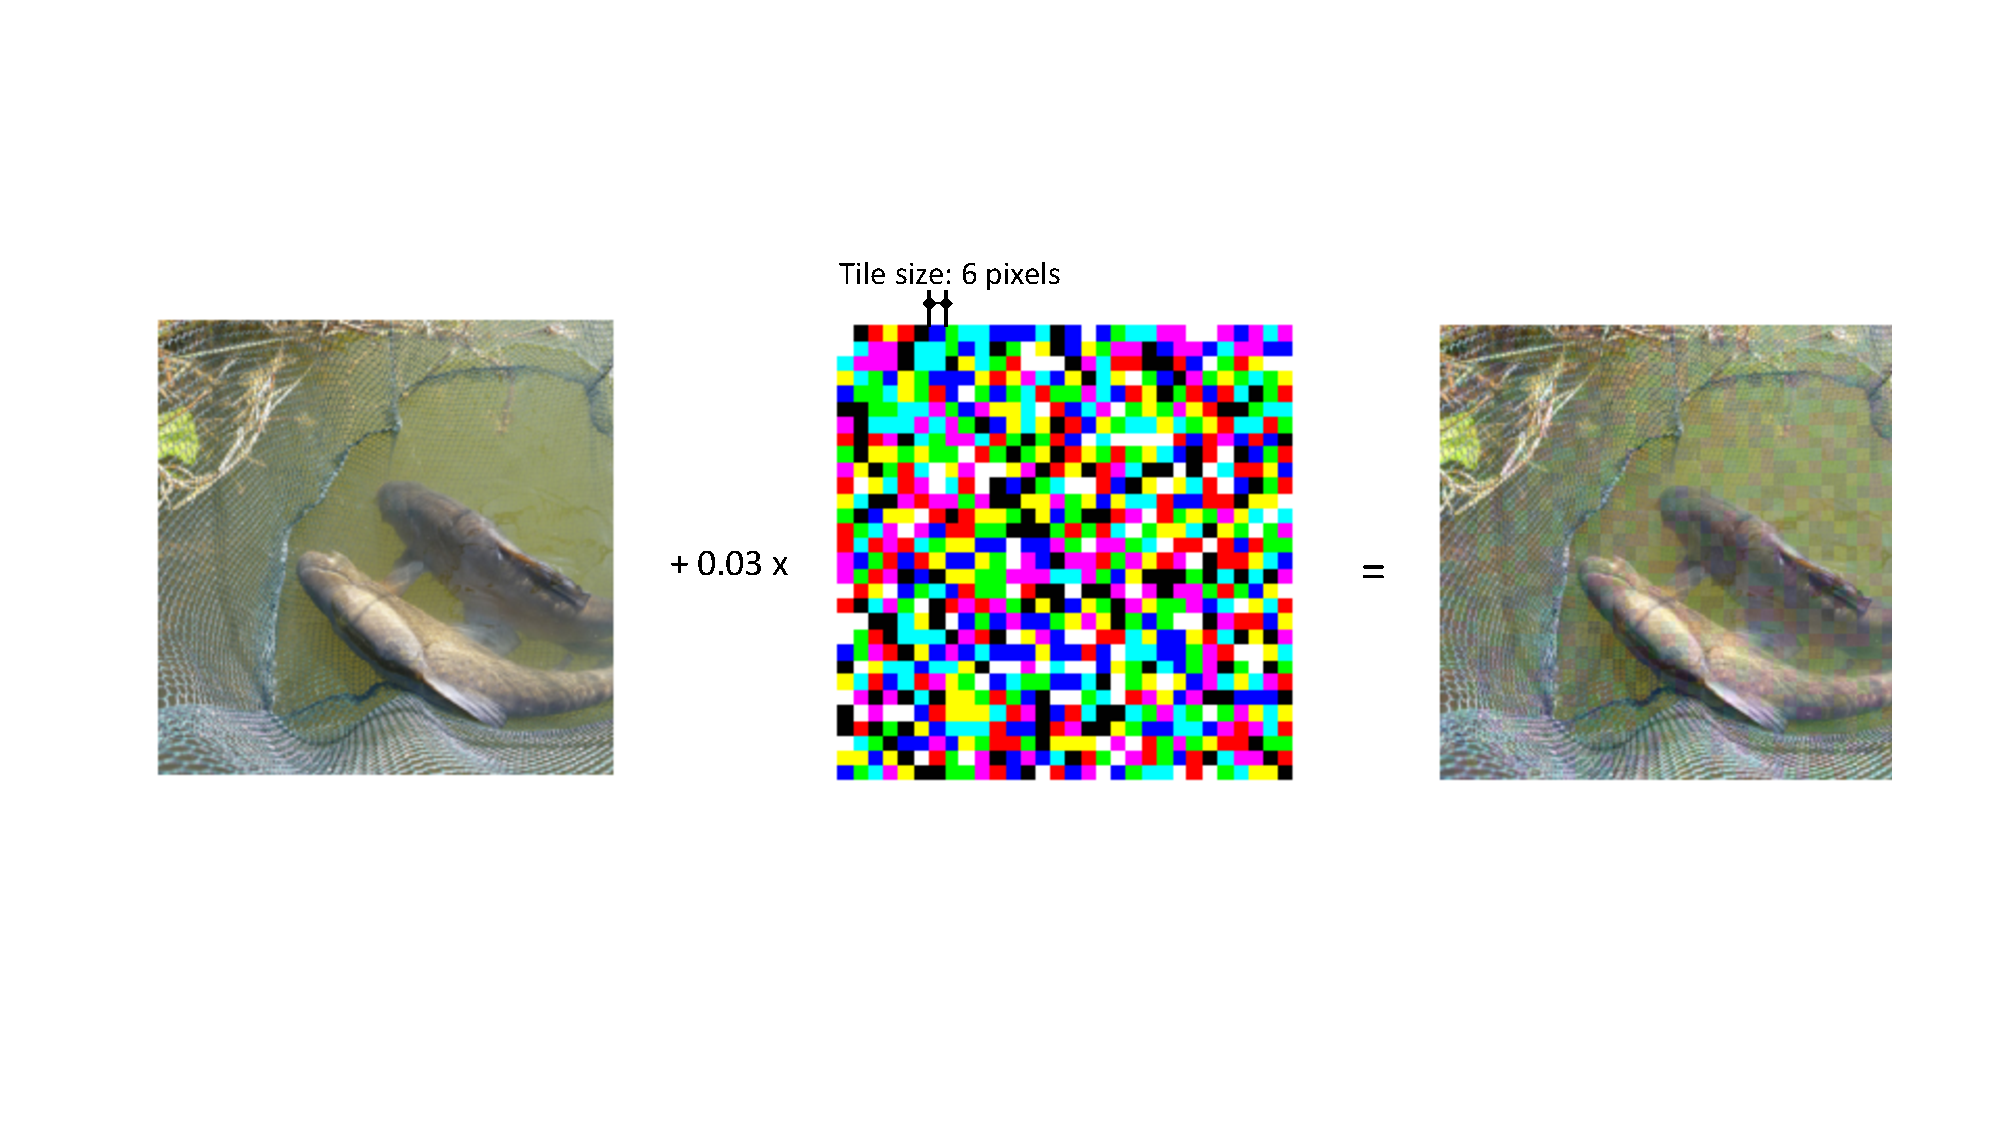
\includegraphics[width=0.8\textwidth]{sections/appendix/arxiv_dfo/images/tile_noise.pdf} \\
    \caption{Illustration of the tiling trick: the same noise is applied on small tile squares.}
    \label{rand}
\end{figure}
\cite{ilyas2018prior} suggested to tile the attack to lower the number of queries necessary to fool the network. Concretely, they observe that the gradient coordinates are correlated for close pixels in the images, so they suggested to add the same noise for small square tiles in the image (see Fig. \ref{rand}). We exploit the same trick since it reduces the dimensionality of the search space, and makes hence evolutionary strategies suited to the problem at hand. Besides breaking the curse of dimensionality, tiling leads surprisingly to a new property that we discovered during our experiments. At a given tiling scale, convolutional neural networks are not robust to random noise. Section~\ref{ahyes} is devoted to this intriguing property. Interestingly enough, initializing our optimization algorithms with a tiled noise at the appropriate scale drastically speeds up the convergence, leading to a reduced number of queries.

%This reduces the dimensionality of the noise space and hence makes evolutionary strategies applicable since they suffer  to scale with the dimensionality of the input space. Moreover we experimentally show that the classifiers are not robust to tiled random noise injection (see Fig. \ref{til}). Since evolution strategies first steps are in general close to random noise addition, the tiling trick  helps to reduce the queries budget. We exploit the same trick in our attacks.
%TODO \url{https://openreview.net/pdf?id=BkMiWhR5K7}
%\todo{Jam: renforcer notre apport/ Done}

\section{Experiments}
\label{expe}
\subsection{General setting and implementation details}
We compare our approach to the ``bandits'' method~\citep{ilyas2018prior} and the parsimonious attack~\citep{moon19aparsimonous}. The latter (parsimonious attack) is, to the best of our knowledge, the state of the art in the black-box setting from the literature; bandits method is also considered in our benchmark given its ties to our models. We reproduced the results from~\citep{moon19aparsimonous} in our setting for fair comparison. As explained in section~\ref{top}, our attacks can be interpreted as $\ell_\infty$ ones. We use the large-scale ImageNet dataset~\citep{imagenet_cvpr09}. As usually done in most frameworks, we quantify our success in terms of attack success rate, median queries and average queries. Here, the number of queries refers to the number of requests to the output logits of a classifier for a given image. For the success rate, we only consider the images that were correctly classified by our model. We use InceptionV3~\citep{szegedy2017inception} , VGG16~\citep{simonyan2014very} with batch normalization (VGG16bn) and ResNet50~\citep{he2016deep}  architectures to measure the performance of our algorithm on the ImageNet dataset. These models reach accuracy close to the the state of the art with around $75-80\%$ for the Top-1 accuracy and $95\%$ for the Top-5 accuracy. We use pretrained models from PyTorch~\citep{paszke2017automatic}. All images are normalized to $\left[0,1\right]$. Results on VGG16bn and ResNet50 are deferred in supplementary material~\ref{other_archi}. The  images to be attacked are selected at random.

We first show that convolutional networks are not robust to tiled random  noise, and more surprisingly that there exists an optimal tile size that is the same for all architectures and noise intensities. Then, we evaluate our methods on both targeted and untargeted objectives. We considered the following losses: the cross entropy $L(f(x),y)=-\log(\mathbb{P}(y|x))$ and a loss inspired from the ``Carlini\&Wagner'' attack: $L(f(x),y)=-\mathbb{P}(y|x)+\max_{y'\neq y}\mathbb{P}(y'|x)$ where $\mathbb{P}(y|x)=\left[\operatorname{Softmax}(f(x))\right]_y$, the probability for the classifier to classify the input $x$ to label $y$. The results for the second loss are deferred in supplementary material~\ref{cwsec}. For all our attacks, we use the Nevergrad~\citep{nevergrad} implementation of evolution strategies. We did not change the default parameters of the optimization strategies.

%\subsection{Ablation study}

\subsection{Convolutional neural networks are not robust to tiled  random noise}\label{ahyes}

\begin{figure}
\centering

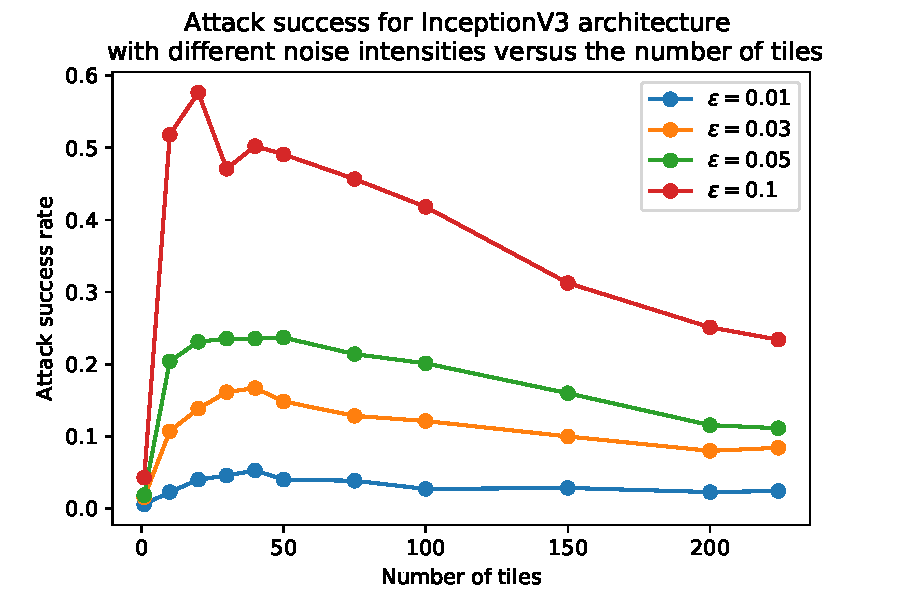
\includegraphics[width=.45\textwidth]{sections/appendix/arxiv_dfo/images/randnoise_inception.pdf}
\includegraphics[width=.45\textwidth]{sections/appendix/arxiv_dfo/images/rand_005.pdf}    

% \includegraphics[width=.3\textwidth]{Master-Template-ICLR2019/images/randnoise_resnet.pdf}
% \includegraphics[width=.3\textwidth]{Master-Template-ICLR2019/images/randnoise_vgg.pdf}
\caption{\label{til}Success rate of a single shot random attacks on ImageNet vs. the number of tiles used to craft the attack. On the left, attacks are plotted against InceptionV3 classifier with different noise intensities ($\epsilon\in\{0.01,0.03,0.05,0.1\}$). On the right, $\epsilon$ is fixed to $0.05$ and the single shot attack is evaluated on InceptionV3, ResNet50 and VGG16bn.}
\end{figure}

In this section, we highlight that neural neural networks are not robust to $\ell_\infty$ tiled random noise. A noise on an image is said to be tiled if the added noise on the image is the same on small squares of pixels (see Figure~\ref{til}). In practice, we divide our image in equally sized tiles.  For each tile, we add to the image a randomly chosen constant noise: $+\epsilon$ with probability $\frac12$ and $-\epsilon$ with probability $\frac12$, uniformly on the tile. The tile trick has been introduced in\cite{ilyas2018black} for dimensionality reduction. Here we exhibit a new behavior that we discovered during our experiments. As shown in Fig. \ref{rand} for reasonable noise intensity ($\epsilon=0.05$), the success rate of a one shot randomly tiled attack is quite high. This fact is observed on many  neural network architectures. We compared the number of tiles since the images input size are not the same for all architectures ($299\times299\times3$ for InceptionV3 and $224\times 224\times3$ for VGG16bn and ResNet50).  The optimal number of tiles (in the sense of attack success rate) is, surprisingly, independent from the architecture and the noise intensity. We also note that the InceptionV3 architecture is more robust to random tiled noise than VGG16bn and ResNet50 architectures. InceptionV3 blocks are parallel convolutions with different filter sizes that are concatenated. Using different filter sizes may attenuate the effect of the tiled noise since some convolution sizes might be less sensitive. We test this with a single random attack with various numbers of tiles (cf. Figure \ref{rand}, \ref{til}). We plotted additional graphs in  supplementary material~\ref{tilsup}.
% \begin{figure}
%     \centering
%     \includegraphics[width=.23\textwidth]{{Master-Template-ICLR2019/images/rand_001.pdf}}
%     \includegraphics[width=.23\textwidth]{Master-Template-ICLR2019/images/rand_003.pdf}
%     \includegraphics[width=.23\textwidth]{Master-Template-ICLR2019/images/rand_005.pdf}    
%     \includegraphics[width=.23\textwidth]{Master-Template-ICLR2019/images/rand_01.pdf}    
%     \caption{X-axis: number of tiles. Y-axis: attack success rate with one single random try. The bound on the $\ell^\infty$ norm of the attack is $0.01$, $0.03$, $0.05$ and $0.1$ respectively.}
%     \label{rand2}
% \end{figure}



\subsection{Untargeted adversarial attacks}
\label{unt_sota}

\begin{figure}
    \centering
    \includegraphics[width=.44\textwidth]{{sections/appendix/arxiv_dfo/images/untargeted_cum.pdf}}
    \includegraphics[width=.44\textwidth]{sections/appendix/arxiv_dfo/images/targeted_cum.pdf}
    \caption{The cumulative success rate in terms the number of queries for the number of queries required for attacks on ImageNet with $\epsilon = 0.05$ in the untargeted (left) and targeted setting (right). The number of queries (x-axis) is plotted with a logarithmic scale.}
    \label{cum}
\end{figure}


\begin{table}[t]
\caption{Comparison of our method with the parsimonious and bandits attacks in the untargeted setting on ImageNet on InceptionV3 pretrained network for $\epsilon=0.05$ and $10,000$ as budget limit.}
\label{untargeted_comp}
\begin{center}
\begin{tabular}{cc|cc|c}
\textbf{Method} & \textbf{\# of tiles} &  \textbf{Average queries} &\textbf{ Median queries }& \textbf{Success rate} \\
 \hline
Parsimonious & - & 702 &222& 98.4\% \\
\hline
Bandits & 30 & 1007 & 269& 95.3\% \\
Bandits & 50 & 995 & 249& 95.1\% \\

\hline
$\operatorname{DFO}_c-\operatorname{Cauchy (1+1)-ES}$ &30&	466& 60	&95.2\%\\
$\operatorname{DFO}_c-\operatorname{Cauchy (1+1)-ES}$&50&	510&	63	&97.3\% \\
\hline
$\operatorname{DFO}_c-\operatorname{DiagonalCMA}$ &30&	533	&189&	97.2\%\\
$\operatorname{DFO}_c-\operatorname{DiagonalCMA}$ &50&	623	&191&	98.7\%\\
\hline
$\operatorname{DFO}_c-\operatorname{CMA}$ & 30&	589	&232	&98.9\%\\
$\operatorname{DFO}_c-\operatorname{CMA}$ & 50&	630	&259&	{\bf{99.2\%}} \\
\hline
$\operatorname{DFO}_d-\operatorname{DiagonalCMA}$  & 30 &  {\bf{424}} & {\bf{20}}& 97.7\%\\

$\operatorname{DFO}_d-\operatorname{DiagonalCMA}$  & 50 & 485 & 38 & 97.4\%\\
\end{tabular}
\end{center}
\end{table}



We first evaluate our attacks in the untargeted setting. The aim is to change the predicted label of the classifier. Following~\citep{moon19aparsimonous,ilyas2018prior}, we use $10,000$ images that are initially correctly classified and we limit the budget to $10,000$ queries. We experimented with 30 and 50 tiles on the images. Only the best performing methods are reported in Table ~\ref{untargeted_comp}.
We compare our results with~\citep{moon19aparsimonous} and~\citep{ilyas2018prior} on InceptionV3 (cf. Table ~\ref{untargeted_comp}). We also plotted the cumulative success rate in terms of required budget in Figure~\ref{cum}. We also evaluated our attacks for smaller noise in supplementary material~\ref{smaller}. We achieve results outperforming or at least equal to  the state of the art in all cases. More remarkably, We improve by far the number of necessary queries to fool the classifiers. The tiling trick partially explains why the average and the median number of queries are low. Indeed, the first queries of our evolution strategies is in general close to random search and hence, according to the observation of Figs ~\ref{rand}-\ref{til}, the first steps are more likely to fool the network, which explains why the queries budget remains low. This Discrete strategies reach better median numbers of queries - which is consistent as we directly search on the limits of the $\ell_\infty$-ball; however, given the restricted search space (only corners of the search space are considered), the success rate is lower and on average the number of queries increases due to hard cases. 

% \begin{table}[t]
% \caption{Comparison of our method with the parsimonious and bandits attacks in the untargeted setting on InceptionV3 pretrained network for $\epsilon=0.05$ and $10,000$ as budget limit. Cont refers to using Eq. \ref{eqcont}, whereas Dis refers to using the discrete counterpart Eq. \ref{eqtoto}.}
% \label{untargeted_comp}
% \begin{center}
% \begin{tabular}{cc|cc|c}
% \textbf{Method} & \textbf{\# of tiles} &  \textbf{Average queries} &\textbf{ Median queries }& \textbf{Success rate} \\
%  \hline
% Parsimonious & - & 722 &237& 98.5\% \\

% Bandits & - & 1107 & 298& 95.1\% \\
% \hline
% cont Cauchy (1+1)-ES &30&	466& 60	&95.2\%\\
% cont Cauchy (1+1)-ES &50&	510&	63	&97.3\% \\
% \hline
% cont DiagonalCMA &30&	533	&189&	97.2\%\\
% cont DiagonalCMA &50&	623	&191&	98.7\%\\
% \hline
% cont CMA & 30&	589	&232	&98.9\%\\
% cont CMA & 50&	630	&259&	99.2\%\\
% \hline
% dis DiagonalCMA & 30 & 424& 20& 97.7\%\\

% dis DiagonalCMA & 50 & 485 & 38 & 97.4\%\\
% \end{tabular}
% \end{center}
% \end{table}

% \begin{figure}
%     \centering
%     \includegraphics[width=.45\textwidth]{{Master-Template-ICLR2019/images/untargeted_cum.pdf}}
%     \includegraphics[width=.45\textwidth]{Master-Template-ICLR2019/images/targeted_cum.pdf}
%     \caption{The cumulative success rate in terms the number of queries for the number of queries required for attacks on ImageNet with $\epsilon = 0.05$ in the untargeted (left) and targeted setting (right). The number of queries (x-axis) is plotted with a logarithmic scale.}
%     \label{cum}
% \end{figure}

% \subsubsection{Untargeted attacks against other architectures}

% We also evaluated our method on different  neural networks architectures. For each network we randomly selected $10,000$ images that were correctly classified. We limit our budget to $10,000$ queries and set the number of tiles to 50. Results with other parameters are deferred to the supplementary material. We achieve a success attack rate up to $100\%$ on every classifier with a budget as low as 8 median queries for the VGG16bn for instance (see Table~\ref{untargeted_archi}). One should notice  that the performances are lower on InceptionV3 as it is also reported for the bandit methods in~\citep{ilyas2018prior}. This possibly due to the fact that the tiling trick is less relevant on the Inception network than on the other networks (see Fig.~\ref{rand2}).




% \begin{table}[t]
% \caption{Comparison of our method on InceptionV3 (I), ResNet50 (R) and VGG16bn (V) for $\epsilon=0.05$ and $10,000$ as budget limit. Cont refers to using Eq. \ref{eqcont}, whereas Dis refers to using the discrete counterpart Eq. \ref{eqtoto}.}
% \label{untargeted_archi}
% \begin{center}
% \begin{tabular}{cc|ccc|ccc|ccc}
% \textbf{Method} &\textbf{Tile size}&\multicolumn{3}{c|}{\textbf{Avg queries}}&\multicolumn{3}{c|}{\textbf{Med. queries}}&\multicolumn{3}{c}{\textbf{Succ. Rate}}\\
% \hline
%  & & I & R & V &  I & R & V&  I & R & V\\
%  \hline
%  cont Cauchy (1+1)-ES &30 & 466&163&86 & 60&19&8 & 95.2\%&99.6\%&100\% \\

% cont Cauchy (1+1)-ES & 50 & 510&218&67& 63&32&4& 97.3\% &99.6\%&99.7\%\\
% \hline
% cont DiagonalCMA & 30 &533&263&174& 189&95&55 & 97.2\%&99.0\%&99.9\%\\
% cont DiagonalCMA & 50 & 623&373&227& 191&121&71 & 98.7\%&99.9\%&100\%\\

% \hline
% cont CMA & 30 &588&256&176& 232&138&72& 98.9\%&99.9\%&99.9\%\\
% cont CMA & 50 & 630&270&219& 259&143&107 & 99.2\%&100\%&99.9\%\\

% \hline
% dis DiagonalCMA & 50 & 485&617&345& 38& 62&6& 97.4\%&99.2\%&99.6\%\\
% dis DiagonalCMA & 30 & 424&417&211& 20&20&2& 97.7\%&98.8\%&99.5\%\\
% \end{tabular}
% \end{center}
% \end{table}


% \subsubsection{With smaller noise intensities}

% We evaluated our method on smaller noise intensities ($\epsilon\in\{0.01,0.03,0.05\}$) in the untargeted setting on ImageNet dataset. In this framework, we also picked up randomly $10,000$ images and limited our budget to $10,000$ queries. We compared to the bandits mehtod~\citep{ilyas2018prior} and to the parsimonious attack~\citep{moon19aparsimonous} on InceptionV3 network. We limited our experiments to a number of tiles of 50. We report our results in Table~\ref{untargeted_epsilon}. We remark our attacks reach state of the art for $\epsilon=0.03$ and $\epsilon=0.05$ both in terms of success rate and queries budget. For $\epsilon=0.01$, we reach results comparable to the state of the art.

% \begin{table}[t]
% \caption{Results of our method compared to the parsimonious and bandit attacks in the untargeted setting on InceptionV3 pretrained network for $\epsilon=0.05$ and a maximum of $10,000$ queries. } 
% \label{untargeted_epsilon}
% \begin{center}
% \begin{tabular}{c|cc|cc|c}
% \textbf{$\epsilon$} &\textbf{Method }&\textbf{ \# of tiles} &  \textbf{Avg. queries} & \textbf{Med. queries} & \textbf{Success rate} \\
%  \hline
% \multirow{5}{*}{$0.05$}&Parsimonious & - & 722 &237& 98.5\% \\
% &Bandits & - & 1107 & 298& 95.1\%  \\
% \cdashline{2-6}
% &cont Cauchy (1+1)-ES &50&	510&	63	&97.3\% \\
% &cont DiagonalCMA &50&	623	&191&	98.7\%\\
% &cont CMA & 50&	630	&259&	99.2\%\\
% &dis DiagonalCMA & 50 & 485 & 38 & 97.4\%\\

% \hline
% \multirow{5}{*}{$0.03$}&Parsimonious & - & 1129 &420&  95.9\% \\
% &Bandits & - & 1382& 520&91.3\%  \\
% \cdashline{2-6}

% &cont Cauchy (1+1)-ES & 50 & 846&	203	&93,2\% \\
% &cont DiagonalCMA & 50 & 971&	429&	96,5\%\\
% &cont CMA &50& 911&	404&	96.7\%\\

% &dis DiagonalCMA & 50 &799&	293&	94,1\% \\

% \hline
% \multirow{5}{*}{$0.01$}&Parsimonious & - & 2141 &1249& 81.3\% \\
% &Bandits & - &2318&1374& 72.4\% \\
% \cdashline{2-6}

% &cont Cauchy (1+1)-ES & 50 & 1668&	751&	72,1\% \\
% &cont DiagonalCMA & 50 & 1958 &1175 & 79.2\%\\
% &cont CMA & 50 & 1921 & 1107 & 80.4\%\\
% &dis DiagonalCMA & 50 & 1188&849&71,3\%\\

% \hline

% \end{tabular}
% \end{center}
% \end{table}




\subsection{Targeted adversarial attacks}

We also evaluate our methods in the targeted case on ImageNet dataset. We selected $1,000$ images, correctly classified. Since the targeted task is harder than the untargeted case, we set the maximum budget to $100,000$ queries, and  $\epsilon=0.05$. We uniformly chose the target class among the incorrect ones. We evaluated our attacks in comparison with the bandits methods~\citep{ilyas2018prior} and the parsimonious attack~\citep{moon19aparsimonous} on InceptionV3 classifier. We also plotted the cumulative success rate in terms of required budget in Figure~\ref{cum}. CMA-ES beats the state of the art on all criteria. DiagonalCMA-ES obtains acceptable results but is less powerful that CMA-ES in this specific case. The classical CMA optimizer is more precise, even if the run time is much longer. Cauchy $(1+1)$-ES and discretized optimization reach good results, but when the task is more complicated they do not reach as good results as the state of the art in black box targeted attacks.
\begin{table}[t]
\caption{Comparison of our method with the parsimonious and bandits attacks in the targeted setting on ImageNet  on InceptionV3 pretrained network for $\epsilon=0.05$ and $100,000$ as budget limit.}
\label{targeted_comp}
\begin{center}
\begin{tabular}{cc|cc|c}
\textbf{Method} &\textbf{ \# of tiles }& \textbf{ Average queries} & \textbf{Median queries} & \textbf{Success rate}\\
 \hline
Parsimonious & - & 7184 &5116& 100\% \\
Bandits &50 &  25341&18053&92.5\% \\
\hline
$\operatorname{DFO}_c-\operatorname{Cauchy (1+1)-ES}$ &50 & 9789 & 6049& 83.2\% \\
$\operatorname{DFO}_c-\operatorname{Diagonal CMA}$& 50 & 6768& {\bf{3797}} & 94.0\%\\
$\operatorname{DFO}_c-\operatorname{CMA}$& 50 & {\bf{6662}} &4692& {\bf{100\%}}\\
\hline
$\operatorname{DFO}_d-\operatorname{Diagonal CMA}$ & 50 & 8957 & 4619 & 64.2\%\\
\end{tabular}
\end{center}
\end{table}

\subsection{Untargeted attacks against an adversarially trained network}

In this section, we experiment our attacks against a defended network by adversarial training~\citep{goodfellow2014explaining}. Since adversarial training is computationally expensive, we restricted ourselves to the CIFAR10 dataset~\citep{krizhevsky2009cifar} for this experiment. Image size is $32\times32\times3$. We adversarially trained a WideResNet28x10~\citep{ZagoruykoK16} with PGD $\ell_\infty$ attacks~\citep{kurakin2016adversarial,madry2018towards} of norm $8/256$ and $10$ steps of size $2/256$. In this setting, we randomly selected $1,000$ images, and  limited the budget to $20,000$ queries. We ran PGD $\ell_\infty$ attacks~\citep{kurakin2016adversarial,madry2018towards} of norm $8/256$ and $20$ steps of size $1/256$ against our network, and achieved a success rate up to $36\%$, which is the the state of the art in the white box setting. We also compared our method to the Parsimonious and bandit attacks. Results are reported in Appendix~\ref{at_comp}. On this task, the parsimonious attack method is slightly better than our best approach.%Our attacks perform a slightly less than the white box PGD attack, but we still fool  results on an adversarially trained network.

% \begin{table}[t]
% \caption{Adversarial attacks against an adversarially trained WideResnet28x10 network on CIFAR10 dataset for $\epsilon=0.03125$ and $20,000$ as budget limit.}
% \label{at_comp}
% \begin{center}
% \begin{tabular}{cc|cc|c}
% \textbf{Method }& \textbf{\# of tiles} & \textbf{ Average queries} &\textbf{ Median queries} &\textbf{ Success rate}\\
%  \hline
% PGD (not black-box)& - & 20 &20& 36\% \\
% \hline
% $\operatorname{DFO}_c-\operatorname{Cauchy (1+1)-ES}$&10& 429& {\bf{60}} &29.5\%\\
% $\operatorname{DFO}_c-\operatorname{Cauchy (1+1)-ES}$ &20 &902&93& 31.5\%\\
% $\operatorname{DFO}_c-\operatorname{Cauchy (1+1)-ES}$&32 &1866& 764& 33.8\%\\
% \hdashline
% $\operatorname{DFO}_c-\operatorname{Diagonal CMA}$ &10&396& 85 &31.5\%\\
% $\operatorname{DFO}_c-\operatorname{Diagonal CMA}$&20 &624& 151& 32.3\% \\
% $\operatorname{DFO}_c-\operatorname{Diagonal CMA}$& 32 &1379 &860& 34.7\%\\
% \hdashline
% $\operatorname{DFO}_c-\operatorname{CMA}$ &10& {\bf{392}} & 87&32.2\%\\
% $\operatorname{DFO}_c-\operatorname{CMA}$&20 &694& 189& 33.5\% \\
% $\operatorname{DFO}_c-\operatorname{CMA}$& 32 &1467 &990& {\bf{35.7\%}}\\
% \end{tabular}
% \end{center}
% \end{table}
% ImageNet results: 10000 images, vgg 16n, top1-acc accuracy 0.73.
% TO ADD: resnet inception
% CIFAR
% \begin{tabular}{|c|c|c|c|c|} 
%   \hline
%     $\epsilon$ & Tile size & Method & Failure rate & Queries (Av/Med)\\
%     \hline
%     0.05& 20 & DiagCMA & 0.67\% & 209/1 \\
%     \hline
%     0.05& 20 & CMA &0.65\% & 290/2 \\
%     \hline
%     0.05& 20 & Bandits &5.31\% & 269/24 \\
%     \hline
%     0.05& 50 & Bandits &5.01\%  & 381/44 \\
%     \hline
% \end{tabular}


















\section{Conclusion}
\label{sec:conc}
In this paper, we proposed a new framework for crafting black box adversarial attacks based on derivative free optimization. Because of the high dimensionality and the characteristics of the problem (see Section~\ref{hypo}), not all optimization strategies give satisfying results. However, combined with the tiling trick, evolutionary strategies such as CMA, DiagonalCMA and  Cauchy (1+1)-ES beats the current state of the art in both targeted and untargeted settings.  In particular, $\operatorname{DFO}_c-\operatorname{CMA}$ improves the state of the art in terms of success rate in almost all settings. We also validated the robustness of our attack against an adversarially trained network. Future work will be devoted to better understanding the intriguing property of the effect that a neural network is not robust to a one shot randomly tiled attack.

% We show the effectiveness of tiled noise and CMA, Diagonal-CMA or Cauchy-$(1+1)$-ES for black-box adversarial attacks. Basically, CMA performs best if the computational cost is not an issue; the Cauchy-$(1+1)$-ES is faster than Diagonal-CMA which is faster than CMA, but top performance is for CMA if we neglect the computational cost and just compare numbers of queries and success rates. In all these methods do not use estimates of the gradient. Results are demonstrated on a wide range of networks and several noise tolerance levels. Results are obtained both by optimizing the attack in a continuous setting (Eq. \ref{eqcont}) and in a discrete setting (Eq. \ref{eqtoto}).
% Section \ref{ahyes} suggests a better robustness of methods combining parallel convolutional blocks; this suggests a direction for defense against adversarial attacks.







%\subsubsection*{Acknowledgments}

%Use unnumbered third level headings for the acknowledgments. All acknowledgments, including those to funding agencies, go at the end of the paper.

\begin{subappendices}
    

\section{Algorithms}
\subsection{The (1+1)-ES algorithm}
\begin{algorithm}
\caption{\label{opo}The $(1+1)$ Evolution Strategy.}
\begin{algorithmic}
\REQUIRE Function $f:\RR^d\to\RR$ to minimize%, number of steps $N$, population size $\lambda$
\STATE $m\leftarrow 0$, $C\leftarrow \boldsymbol{I}_d$, $\sigma\leftarrow 1$
\FOR{$t=1 ...n$}
\STATE (Generate candidates)
\STATE Generate $m' \sim m+\sigma X$ where $X$ is sampled from a Cauchy or Gaussian distribution.
\IF{$f(m')\leq f(m)$}
\STATE{$m\leftarrow m'$, $\sigma\leftarrow 2\sigma$}
\ELSE
\STATE{$\sigma\leftarrow 2^{-\frac14}\sigma$}
\ENDIF
\ENDFOR
\end{algorithmic}
\end{algorithm}

\subsection{CMA-ES algorithm}
\begin{algorithm}
\caption{\label{cmaalg}CMA-ES algorithm. The $T$ subscript denotes transposition.}
\begin{algorithmic}
\REQUIRE Function $f:\RR^d\to\RR$ to minimize, parameters $b$, $c$, $w_1>\dots,w_\mu>0$, $p_c$ and others as in e.g. \citep{HAN}.%, number of steps $N$, population size $\lambda$
\STATE $m\leftarrow 0$, $C\leftarrow \boldsymbol{I}_d$, $\sigma\leftarrow 1$
\FOR{$t=1 ...n$}
%\STATE (Generate candidates)
\STATE Generate $x_1,...,x_\lambda \sim m + \sigma \mathcal{N}(0,C)$.
\STATE Define $x'_{i}$ the $i^{th}$ best of the $x_i$.
%\STATE Cumulation for the covariance, i.e. increase $p_c$ if $p_c<1.5\sqrt{dimension}$ and the $\mu$ best points are far enough from $m$
\STATE{Update the cumulation for $C$: $p_c\leftarrow\mbox{ cumulation of }p_c$, overall direction of progress.}
\STATE Update the covariance matrix:
$$C\leftarrow (1-c)\underbrace{C}_{inertia}+\frac cb \underbrace{(p_c\times p_c^T)}_{\mbox{overall direction}} +c(1-\frac 1b)\sum_{i=1}^\mu w_i\underbrace{\frac{x'_i-m}\sigma\times \frac{(x'_i-m)^T}\sigma}_{\mbox{``covariance'' of the $\frac1\sigma x'_i$}}$$
\STATE Update mean:% candidates)
$$m\leftarrow \sum_{i=1}^\mu w_i x_{i:\lambda}$$
\STATE Update $\sigma$ by cumulative step-size adaptation~\citep{csalinear}.
%$$\sigma\leftarrow \sigma \times \exp(\frac cd ( || ) ).$$ too complicated
\ENDFOR
\end{algorithmic}
\end{algorithm}

\newpage
\section{Additional plots for the tiling trick}
\label{tilsup}
\begin{figure}[htb]
\centering
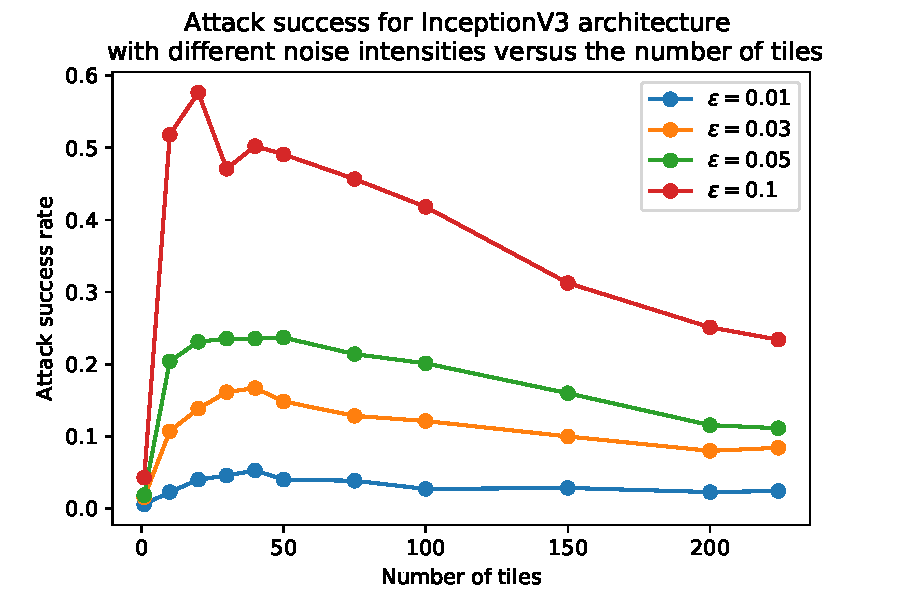
\includegraphics[width=.3\textwidth]{sections/appendix/arxiv_dfo/images/randnoise_inception.pdf}
\includegraphics[width=.3\textwidth]{sections/appendix/arxiv_dfo/images/randnoise_resnet.pdf}
\includegraphics[width=.3\textwidth]{sections/appendix/arxiv_dfo/images/randnoise_vgg.pdf}\\
\caption{\label{til1}Random attack success rate against InceptionV3 (left), ResNet50 (center), VGG16bn (right) for different noise intensities. We just randomly draw one tiled attack and check if it is successful.}
\end{figure}

\begin{figure}[htb]
\centering
\includegraphics[width=.23\textwidth]{sections/appendix/arxiv_dfo/images/rand_001.pdf}
\includegraphics[width=.23\textwidth]{sections/appendix/arxiv_dfo/images/rand_003.pdf}
\includegraphics[width=.23\textwidth]{sections/appendix/arxiv_dfo/images/rand_005.pdf}
\includegraphics[width=.23\textwidth]{sections/appendix/arxiv_dfo/images/rand_01.pdf}\\
\caption{\label{til2}Random attack success rate for different noise intensities $\epsilon\in\{0.01,0.03,0.05,0.1\}$ (from right to left) against different architectures. We just randomly draw one tiled attack and check if it is successful.}
\end{figure}

\section{Results with ``Carlini\&Wagner'' loss}
\label{cwsec}
In this section, we follow the same experimental setup as in Section~\ref{unt_sota}, but we built our attacks with the ``Carlini\&Wagner'' loss instead of the cross entropy. We remark the results are comparable and similar.

\begin{table}[htb]
\caption{Comparison of our method with``Carlini\&Wagner'' loss versus the parsimonious and bandits attacks in the untargeted setting on InceptionV3 pretrained network for $\epsilon=0.05$ and $10,000$ as budget limit. }
\label{untargeted_cw}
\begin{center}
\begin{tabular}{cc|cc|c}
\textbf{Method} & \textbf{\# of tiles} &  \textbf{Average queries} &\textbf{ Median queries }& \textbf{Success rate} \\
\hline
$\operatorname{DFO}_c-\operatorname{Cauchy (1+1)-ES}$ & 30&353	&57	&97.2\%\\
$\operatorname{DFO}_c-\operatorname{Cauchy (1+1)-ES}$ &50&\textbf{347}&	63&	98.8\%\\

\hline

$\operatorname{DFO}_c-\operatorname{DiagonalCMA}$ & 30&	483	&167&	98.8\%\\
$\operatorname{DFO}_c-\operatorname{DiagonalCMA}$  & 50&	528	&181&	99.2\%\\


\hline
$\operatorname{DFO}_c-\operatorname{CMA}$ & 30&	475	&225&	99.2\%\\
$\operatorname{DFO}_c-\operatorname{CMA}$ & 50&	491	&246	&\textbf{99.4\%}\\

\hline
$\operatorname{DFO}_d-\operatorname{DiagonalCMA}$  &30&	482 &	\textbf{27}&	98.0\%\\
$\operatorname{DFO}_d-\operatorname{DiagonalCMA}$  &50&	510& 37	&	98.0\%\\
\end{tabular}
\end{center}
\end{table}



\newpage
\section{Untargeted attacks with smaller noise intensities}
\label{smaller}
We evaluated our method on smaller noise intensities ($\epsilon\in\{0.01,0.03,0.05\}$) in the untargeted setting on ImageNet dataset. In this framework, we also picked up randomly $10,000$ images and limited our budget to $10,000$ queries. We compared to the bandits method~\citep{ilyas2018prior} and to the parsimonious attack~\citep{moon19aparsimonous} on InceptionV3 network. We limited our experiments to a number of tiles of 50. We report our results in Table~\ref{untargeted_epsilon}. We remark our attacks reach state of the art for $\epsilon=0.03$ and $\epsilon=0.05$ both in terms of success rate and queries budget. For $\epsilon=0.01$, we reach results comparable to the state of the art.

\begin{table}[htb]
\caption{Results of our method compared to the parsimonious and bandit attacks in the untargeted setting on InceptionV3 pretrained network for different values of noise intensities $\epsilon\in\{0.01,0.03,0.05\}$ and a maximum of $10,000$ queries. } 
\label{untargeted_epsilon}
\begin{center}
\begin{tabular}{c|cc|cc|c}
\textbf{$\epsilon$} &\textbf{Method }&\textbf{ \# of tiles} &  \textbf{Avg. queries} & \textbf{Med. queries} & \textbf{Success rate} \\
 \hline
\multirow{5}{*}{$0.05$}&Parsimonious & - & 722 &237& 98.5\% \\
% \cdashline{2-6}
&Bandits & 50 & 995 & 249& 95.1\% \\
% \cdashline{2-6}
&$\operatorname{DFO}_c-\operatorname{Cauchy (1+1)-ES}$ &50&	510&	63	&97.3\% \\
&$\operatorname{DFO}_c-\operatorname{DiagonalCMA}$  &50&	623	&191&	98.7\%\\
&$\operatorname{DFO}_c-\operatorname{CMA}$  & 50&	630	&259&	\textbf{99.2\%}\\
&$\operatorname{DFO}_d-\operatorname{DiagonalCMA}$  & 50 & \textbf{485} & \textbf{38} & 97.4\%\\

\hline
\multirow{5}{*}{$0.03$}&Parsimonious & - & 1104 &392&  95.7\% \\
% \cdashline{2-6}

&Bandits & 50 & 1376& 466&92.7\%  \\
% \cdashline{2-6}

&$\operatorname{DFO}_c-\operatorname{Cauchy (1+1)-ES}$ & 50 & 846&	\textbf{203}	&93,2\% \\
&$\operatorname{DFO}_c-\operatorname{DiagonalCMA}$ & 50 & 971&	429&	96,5\%\\
&$\operatorname{DFO}_c-\operatorname{CMA}$ &50& 911&	404&	\textbf{96.7\%}\\

&$\operatorname{DFO}_d-\operatorname{DiagonalCMA}$  & 50 &\textbf{799}&	293&	94,1\% \\

\hline
\multirow{5}{*}{$0.01$}&Parsimonious & - & 2104 &1174& 80.3\% \\
% \cdashline{2-6}
&Bandits & 50 &2018&992& 72.9\% \\
% \cdashline{2-6}

&$\operatorname{DFO}_c-\operatorname{Cauchy (1+1)-ES}$& 50 & 1668&	\textbf{751}&	72,1\% \\
&$\operatorname{DFO}_c-\operatorname{DiagonalCMA}$ & 50 & 1958 &1175 & 79.2\%\\
&$\operatorname{DFO}_c-\operatorname{CMA}$& 50 & 1921 & 1107 & \textbf{80.4\%}\\
&$\operatorname{DFO}_d-\operatorname{DiagonalCMA}$ & 50 & \textbf{1188} &849&71,3\%\\

\hline

\end{tabular}
\end{center}
\end{table}


\newpage

% \section{Table for attacks against adversarially tranined network}
% \begin{table}[htb]
% \caption{Adversarial attacks against an adversarially trained WideResnet28x10 network on CIFAR10 dataset for $\epsilon=0.03125$ and $20,000$ as budget limit.}
% \label{at_comp}
% \begin{center}
% \begin{tabular}{cc|cc|c}
% \textbf{Method }& \textbf{\# of tiles} & \textbf{ Average queries} &\textbf{ Median queries} &\textbf{ Success rate}\\
%  \hline
% PGD (not black-box)& - & 20 &20& 36\% \\
% \hline
% $\operatorname{DFO}_c-\operatorname{Cauchy (1+1)-ES}$&10& 429& {\bf{60}} &29.5\%\\
% $\operatorname{DFO}_c-\operatorname{Cauchy (1+1)-ES}$ &20 &902&93& 31.5\%\\
% $\operatorname{DFO}_c-\operatorname{Cauchy (1+1)-ES}$&32 &1866& 764& 33.8\%\\
% \hdashline
% $\operatorname{DFO}_c-\operatorname{Diagonal CMA}$ &10&396& 85 &31.5\%\\
% $\operatorname{DFO}_c-\operatorname{Diagonal CMA}$&20 &624& 151& 32.3\% \\
% $\operatorname{DFO}_c-\operatorname{Diagonal CMA}$& 32 &1379 &860& 34.7\%\\
% \hdashline
% $\operatorname{DFO}_c-\operatorname{CMA}$ &10& {\bf{392}} & 87&32.2\%\\
% $\operatorname{DFO}_c-\operatorname{CMA}$&20 &694& 189& 33.5\% \\
% $\operatorname{DFO}_c-\operatorname{CMA}$& 32 &1467 &990& {\bf{35.7\%}}\\
% \end{tabular}
% \end{center}
% \end{table}

% \newpage
\section{Untargeted attacks against other architectures}
\label{other_archi}

We also evaluated our method on different  neural networks architectures. For each network we randomly selected $10,000$ images that were correctly classified. We limit our budget to $10,000$ queries and set the number of tiles to 50. 
We achieve a success attack rate up to $100\%$ on every classifier with a budget as low as 8 median queries for the VGG16bn for instance (see Table~\ref{untargeted_archi}). One should notice  that the performances are lower on InceptionV3 as it is also reported for the bandit methods in~\citep{ilyas2018prior}. This possibly due to the fact that the tiling trick is less relevant on the Inception network than on the other networks (see Fig.~\ref{til}).




\begin{table}[htb]
\caption{Comparison of our method on the ImageNet dataset with InceptionV3 (I), ResNet50 (R) and VGG16bn (V) for $\epsilon=0.05$ and $10,000$ as budget limit.}
\label{untargeted_archi}
\begin{center}
\begin{tabular}{cc|ccc|ccc|ccc}
\textbf{Method} &\textbf{Tile size}&\multicolumn{3}{c|}{\textbf{Avg queries}}&\multicolumn{3}{c|}{\textbf{Med. queries}}&\multicolumn{3}{c}{\textbf{Succ. Rate}}\\
\hline
 & & I & R & V &  I & R & V&  I & R & V\\
 \hline
$\operatorname{DFO}_c-\operatorname{Cauchy (1+1)-ES }$ &30 & 466&\textbf{163}&86 & 60&\textbf{19}&8 & 95.2\%&99.6\%&\textbf{100\% }\\

$\operatorname{DFO}_c-\operatorname{Cauchy (1+1)-ES }$ & 50 & 510&218&\textbf{67}& 63&32&4& 97.3\% &99.6\%&99.7\%\\
\hline
$\operatorname{DFO}_c-\operatorname{DiagonalCMA}$& 30 &533&263&174& 189&95&55 & 97.2\%&99.0\%&99.9\%\\
$\operatorname{DFO}_c-\operatorname{DiagonalCMA}$ & 50 & 623&373&227& 191&121&71 & 98.7\%&99.9\%&\textbf{100\%}\\

\hline
$\operatorname{DFO}_c-\operatorname{CMA}$& 30 &588&256&176& 232&138&72& 98.9\%&99.9\%&99.9\%\\
$\operatorname{DFO}_c-\operatorname{CMA}$ & 50 & 630&270&219& 259&143&107 & \textbf{99.2\%}&\textbf{100\%}&99.9\%\\

\hline
$\operatorname{DFO}_d-\operatorname{DiagonalCMA}$& 50 & 485&617&345& 38& 62&6& 97.4\%&99.2\%&99.6\%\\
$\operatorname{DFO}_d-\operatorname{DiagonalCMA}$ & 30 & \textbf{424}&417&211& \textbf{20}&20&\textbf{2}& 97.7\%&98.8\%&99.5\%\\
\end{tabular}
\end{center}
\end{table}


\newpage


\section{Table for attacks against adversarially tranined network}
\begin{table}[htb]
\caption{Adversarial attacks against an adversarially trained WideResnet28x10 network on CIFAR10 dataset for $\epsilon=0.03125$ and $20,000$ as budget limit.}
\label{at_comp}
\begin{center}
\begin{tabular}{cc|cc|c}
\textbf{Method }& \textbf{\# of tiles} & \textbf{ Average queries} &\textbf{ Median queries} &\textbf{ Success rate}\\
 \hline
PGD (not black-box)& - & 20 &20& 36\% \\
\hline

Parsimonious&-&1130 & 450&\bf{42\%}\\
\hline
Bandits&10& 1429& {530} &29.1\%\\
 Bandits&20 &1802&798& 33.8\%\\
Bandits&32 &1993& 812& 34.8\%\\
\hline
$\operatorname{DFO}_c-\operatorname{Cauchy (1+1)-ES}$&10& 429& {\bf{60}} &29.5\%\\
$\operatorname{DFO}_c-\operatorname{Cauchy (1+1)-ES}$& 20&902 & 93  &30.5\%\\
$\operatorname{DFO}_c-\operatorname{Cauchy (1+1)-ES}$&32 &1865 &764 & 31.7\%\\
% \hdashline
$\operatorname{DFO}_c-\operatorname{Diagonal CMA}$ &10&395 &85&30.5\%\\
$\operatorname{DFO}_c-\operatorname{Diagonal CMA}$&20 &624& 151& 31.3\% \\
$\operatorname{DFO}_c-\operatorname{Diagonal CMA}$& 32 &1379 &860& 34.7\%\\
% \hdashline
$\operatorname{DFO}_c-\operatorname{CMA}$ &10& {\bf{363}} & 156&30.4\%\\
$\operatorname{DFO}_c-\operatorname{CMA}$&20 &1676&740& 40.2\% \\
$\operatorname{DFO}_c-\operatorname{CMA}$& 32 &2311 &1191& 40.2\%\\
\end{tabular}
\end{center}
\end{table}

\newpage


\section{Failing methods}

In this section, we compare our attacks to other optimization strategies. We run our experiments in the same setup as in Section~\ref{unt_sota}. Results are reported in Table~\ref{untargeted_fail}. DE and Normal (1+1)-ES performs poorly, probably because these optimization strategies converge slower when the optima are at ``infinity''.  We reformulate this sentence accordingly in the updated version of the paper. Finally, as the initialization of Powell is linear with the dimension and with less variance, it performs poorer than simple random search. Newuoa, SQP and Cobyla algorithms have also been tried on a smaller number images (we did not report the results), but their initialization is also linear in the dimension, so they reach very poor results too.

\begin{table}[htb]
\caption{Comparison with other DFO optimization strategies in the untargeted setting on ImageNet dataset InceptionV3 pretrained network for $\epsilon=0.05$ and $10,000$ as budget limit.}
\label{untargeted_fail}
\begin{center}
\begin{tabular}{cc|cc|c}
\textbf{Method} & \textbf{\# of tiles} &  \textbf{Average queries} &\textbf{ Median queries }& \textbf{Success rate} \\
 \hline

$\operatorname{DFO}_c-\operatorname{Cauchy (1+1)-ES }$ &30&	466& 60	&95.2\%\\
$\operatorname{DFO}_c-\operatorname{Cauchy (1+1)-ES }$ &50&	510&	63	&97.3\% \\
\hline
$\operatorname{DFO}_c-\operatorname{DiagonalCMA}$ &30&	533	&189&	97.2\%\\
$\operatorname{DFO}_c-\operatorname{DiagonalCMA}$ &50&	623	&191&	98.7\%\\
\hline

$\operatorname{DFO}_c-\operatorname{CMA}$& 30&	589	&232	&98.9\%\\
$\operatorname{DFO}_c-\operatorname{CMA}$ & 50&	630	&259&	99.2\%\\

\hline

$\operatorname{DFO}_c-\operatorname{DE}$ & 30&756&159&78.8\%\\
$\operatorname{DFO}_c-\operatorname{DE}$ & 50&699&149	&76.0\%\\
\hline

$\operatorname{DFO}_c-\operatorname{Normal(1+1)-ES}$ &30&	581&	45	&87.6\%\\
$\operatorname{DFO}_c-\operatorname{Normal(1+1)-ES}$ &50&661&66&92.8\%\\
\hline

$\operatorname{DFO}_c-\operatorname{RandomSearch}$  &30&	568	&6	&37.9\%\\
$\operatorname{DFO}_c-\operatorname{RandomSearch}$ &50&	527	&5&	38.2\%\\
\hline
$\operatorname{DFO}_c-\operatorname{Powell}$ &30&	4889&	5332&	14.4\%\\
$\operatorname{DFO}_c-\operatorname{Powell}$ &50&	4578	&4076&	7.3\%\\



\end{tabular}
\end{center}
\end{table}

\end{subappendices}





\newcommand{\todo}[2]{{\color{red}{\bf TODO (#1):} #2}}
\newcommand{\todoben}[1]{\todo{ben}{#1}}
\newcommand{\todoalex}[1]{\todo{alex}{#1}}
\newcommand{\todolau}[1]{\todo{lau}{#1}}
\newcommand{\todoraf}[1]{\todo{raf}{#1}}


\newtheorem{method}{Attack}
\newcommand{\E}{\mathbb{E}}




\chapter{Advocating for Multiple Defense Strategies against Adversarial Examples}
\label{paper:ecml_rat}

It has been empirically observed that defense mechanisms designed to protect neural networks against $\ell_\infty$ adversarial examples offer poor performance against $\ell_2$ adversarial examples and vice versa. In this paper we conduct a geometrical analysis that validates this observation. Then, we provide a number of empirical insights to illustrate the effect of this phenomenon in practice. 
Then, we review some of the existing defense mechanism that attempts to defend against multiple attacks by mixing defense strategies. Thanks to our numerical experiments, we discuss the relevance of this method and state open questions for the adversarial examples community.



\section{Introduction}
\label{intro}
Deep neural networks achieve state-of-the-art performances in a variety of domains such as natural language processing~\cite{radford2018Language}, image recognition~\cite{he2016deep} and speech
recognition~\cite{hinton2012deep}. However, it has been shown that such neural networks are vulnerable to {\em adversarial examples}, \emph{i.e.}, imperceptible variations of the natural examples, crafted to deliberately mislead the models~\cite{globerson2006nightmare,biggio2013evasion,Szegedy2013IntriguingPO}. Since their discovery, a variety of algorithms have been developed to generate adversarial examples (a.k.a. attacks), for example FGSM \citep{goodfellow2014explaining}, PGD \citep{madry2018towards} and C\&W \citep{carlini2017towards}, to mention the most popular ones.

Because it is difficult to characterize the space of visually imperceptible variations of a natural image, existing adversarial attacks use surrogates that can differ from one attack to another. For example, \cite{goodfellow2014explaining} use the $\ell_\infty$ norm to measure the distance between the original image and the adversarial image whereas \cite{carlini2017towards} use the $\ell_2$ norm.  When the input dimension is low, the choice of the norm is of little importance because the $\ell_\infty$ and $\ell_2$ balls overlap by a large margin, and the adversarial examples lie in the same space. An important insight in this paper is to observe that the overlap between the two balls  diminishes exponentially quickly as the dimensionality of the input space increases. For typical image datasets with large dimensionality, the two balls are mostly disjoint. As a consequence, the $\ell_\infty$ and the $\ell_2$ adversarial examples lie in different areas of the space, and it explains why $\ell_\infty$ defense mechanisms perform poorly against $\ell_2$ attacks and vice versa. 

Building on this insight, we advocate for designing models that incorporate defense mechanisms against both $\ell_\infty$ and $\ell_2$ attacks and review several ways of mixing existing defense mechanisms. In particular, we evaluate the performance of  {\em Mixed Adversarial Training} (MAT)~\cite{goodfellow2014explaining} which consists of  augmenting training batches using \emph{both} $\ell_\infty$ and $\ell_2$ adversarial examples, and {\em Randomized Adversarial Training} (RAT)~\cite{salman2019provably}, a solution to benefit from the advantages of both $\ell_\infty$ adversarial training, and $\ell_2$ randomized defense. 


\paragraph{Outline.} The rest is organized as follows. In Section~\ref{sec:preliminaries_rat}, we recall the principle of existing attacks and defense mechanisms. In Section~\ref{sec:no_free_lunch}, we conduct a theoretical analysis to show why  the $\ell_\infty$ defense mechanisms cannot be robust against $\ell_2$ attacks and vice versa. We then corroborate this analysis with empirical results using real adversarial attacks and defense mechanisms. In Section~\ref{sec:building_defense_mechanisms}, we discuss various strategies to mix defense mechanisms, conduct comparative experiments, and discuss the performance of each strategy. 



\section{Preliminaries on Adversarial Attacks and Defenses}
\label{sec:preliminaries_rat}

Let us first consider a standard classification task with an input space $\mathcal{X}=[0,1]^d$ of dimension $d$,  an output space $\mathcal{Y}=[K]$ and a data distribution $\mathcal D$ over $\mathcal X \times \mathcal Y$. We assume the model $f_\theta$ has been trained to minimize the expectation over $\mathcal{D}$ of a loss function $\mathcal{L}$ as follows:
\begin{equation}
    \min_{\theta} \mathbb{E}_{(x,y) \sim \mathcal{D}} \left[ \mathcal{L}(f_\theta(x), y) \right]. 
    \label{eqn:classification}
\end{equation}

\subsection{Adversarial attacks}
\label{subsec:adversarial_attacks}
 
Given an input-output pair $(x,y) \sim \mathcal{D}$, an {\em adversarial attack} is a procedure that produces a small perturbation $\tau \in  \mathcal X$  such that $f_\theta(x + \tau) \neq y$. To find the best perturbation $\tau$, existing attacks can adopt one of the two following strategies:  (i)  maximizing the loss $\mathcal L(f_\theta(x + \tau), y)$ under some constraint on $\lVert\tau\rVert_p$\footnote{with $p \in \{0, \cdots, \infty\}$.} (a.k.a. loss maximization); or (ii)  minimizing $\lVert\tau\rVert_p$ under some constraint on the loss $\mathcal L(f_\theta(x + \tau), y)$ (a.k.a. perturbation minimization). 

\paragraph{(i) Loss maximization.} In this scenario, the procedure maximizes the loss objective function, under the constraint that the $\ell_p$ norm of the perturbation remains bounded by some value $\epsilon$, as follows:  

\begin{equation}
  \argmaxB_{\lVert\tau\rVert_p \leq \epsilon} \mathcal{L}(f_\theta(x+\tau),y).
  \label{eqn::lossmax}
\end{equation}

The typical value of $\epsilon$ depends on the norm $\lVert\cdot\rVert_p$ considered in the problem setting. In order to compare $\ell_\infty$ and $\ell_2$ attacks of similar strength, we choose values of $\epsilon_\infty$ and $\epsilon_2$ (for $\ell_\infty$ and $\ell_2$ norms respectively) which result in $\ell_\infty$ and $\ell_2$ balls of equivalent volumes. For the particular case of CIFAR-10, this would lead us to choose $\epsilon_\infty = 0.03$ and $\epsilon_2 = 0.8$ which correspond to the maximum values chosen empirically to avoid the generation of visually detectable perturbations. 
The current state-of-the-art method to solve Problem~(\ref{eqn::lossmax}) is based on a projected gradient descent (PGD)~\cite{madry2018towards} of radius~$\epsilon$. Given a budget $\epsilon$, it recursively computes
\begin{equation}
    x^{t+1}=\prod_{B_p(x,\epsilon)}\left(x^t
+\alpha \argmaxB_{\delta\text{ s.t. }||\delta||_p\leq1} \left(\Delta^t|\delta \right)\right)
    \label{eqn::projectionPGD}
\end{equation}
where $B_p(x,\epsilon) = \{ x+\tau \text{~s.t.~} \lVert\tau\rVert_p \leq \epsilon\}$, $\Delta^t=\nabla_x\mathcal{L}\left(f_\theta\left(x^t\right),y\right)$, $\alpha$ is a gradient step size, and $\prod_S$ is the projection operator on $S$. Both PGD attacks with $p=2$, and $p=\infty$ are currently used in the literature as state-of-the-art attacks for the loss maximization problem. 


\paragraph{(ii) Perturbation minimization.}  This type of procedure search for the perturbation that has the minimal $\ell_p$ norm, under the constraint that $\mathcal{L}(f_\theta(x+\tau),y)$ is bigger than a given bound $c$:
    \begin{equation}
      \argminB_{\mathcal{L}(f_\theta(x+\tau),y) \geq c} 
      \lVert\tau\rVert_p.
      \label{eqn::normmin}
  \end{equation}
  The value of $c$ is typically chosen depending on the loss function $\mathcal{L}$\footnote{For example, if $\mathcal{L}$ is the $0/1$ loss, any $c>0$ is acceptable.}.
  Problem~(\ref{eqn::normmin}) has been tackled in~\cite{carlini2017towards}, leading to the following method, denoted C\&W attack in the rest of this appendix. It aims at solving the following Lagrangian relaxation of Problem~(\ref{eqn::normmin}):
  \begin{equation}
    \argminB_{\tau} \lVert\tau\rVert_p+ \lambda \times g(x+\tau)
    \label{eqn::CWproblem}
\end{equation}
where $g(x+\tau)<0$ if and only if $\mathcal{L}(f_\theta(x+\tau),y) \geq c$. 
The authors use a change of variable $\tau=\tanh(w)-x$ to ensure that $-1 \leq x+\tau \leq 1$, a binary search to optimize the constant $c$, and Adam or SGD to compute an approximated solution. The C\&W attack is well defined both for $p=2$, and $p=\infty$, but there is a clear empirical gap of efficiency in favor of the $\ell_2$ attack.

In this appendix, we focus on the {\em Loss Maximization} setting using the PGD attack. However we  conduct some of our experiments using {\em Perturbation Minimization} algorithms such as C\&W to capture more detailed information about the location of adversarial examples in the vector space\footnote{As it has a more flexible geometry than the {\em Loss Maximization} attacks.}. 

\subsection{Defense mechanisms}
\label{subsec:defense_mechanisms}

\paragraph{Adversarial Training (AT).}
\label{paragraph:adversarial_training}

Adversarial Training was introduced in \cite{goodfellow2014explaining} and later improved in \cite{madry2018towards} as a first defense mechanism to train robust neural networks. It consists in augmenting training batches with adversarial examples generated during the training procedure. The standard training procedure from Equation~(\ref{eqn:classification}) is thus replaced by the following  $\min$ $\max$ problem, where the classifier tries to minimize the expected loss under maximum perturbation of its input:
\begin{equation}
    \min_{\theta}\mathbb{E}_{(x, y)\sim \mathcal{D}} \left[ \max_{\lVert\tau\rVert_p \leq \epsilon} \mathcal{L} \left( f_{\theta}(x+\tau), y \right) \right].
\end{equation}
\noindent
In the case where $p=\infty$, this technique offers good robustness  against $\ell_\infty$ attacks \cite{athalye2018obfuscated}. AT can also be used with $\ell_2$ attacks but as we will discuss in Section~\ref{sec:no_free_lunch}, AT with one norm offers poor protection against the other.
The main weakness of Adversarial Training is its lack of formal guarantees. Despite some recent work providing great insights \cite{sinha2017certifying,zhang2019theoretically}, there is no worst case lower bound yet on the accuracy under attack of this method.


\paragraph{Noise injection mechanisms (NI).}\label{subsec:randomized_training}



Another important technique to defend against adversarial examples is to use Noise Injection. 
In contrast with Adversarial Training, Noise Injection mechanisms are usually deployed after training. In a nutshell, it works as follows. At inference time, given a unlabeled sample $x$, the network outputs
\begin{equation}
    \tilde{f}_\theta (x):= f_\theta(x + \eta) \ \ \ (\text{instead of  }f_\theta(x)) 
\end{equation}
where $\eta$ is a random variable on $\mathbb{R}^d$.
Even though, Noise Injection is often less efficient than Adversarial Training in practice (see \emph{e.g.}, Table~\ref{tab:results}), it benefits from strong theoretical background. In particular, recent work \cite{lecuyer2018certified}, followed by \cite{KolterRandomizedSmoothing,pinot2019theoretical} demonstrated that noise injection from a Gaussian distribution can give provable defense against $\ell_2$ adversarial attacks. In this work, besides the classical Gaussian noises already investigated in previous works, we evaluate the efficiency of Uniform distributions to defend against $\ell_2$ adversarial examples. 


\section{No Free Lunch for Adversarial Defenses}
\label{sec:no_free_lunch}

In this Section, we show both theoretically and empirically that defenses mechanisms intending to defend against $\ell_\infty$ attacks cannot provide suitable defense against $\ell_2$ attacks. Our reasoning is perfectly general; hence we can similarly demonstrate the reciprocal statement, but we focus on this side for simplicity. 

\begin{figure*}[ht]
  \centering
  \begin{minipage}{.32\linewidth}
    \centering
    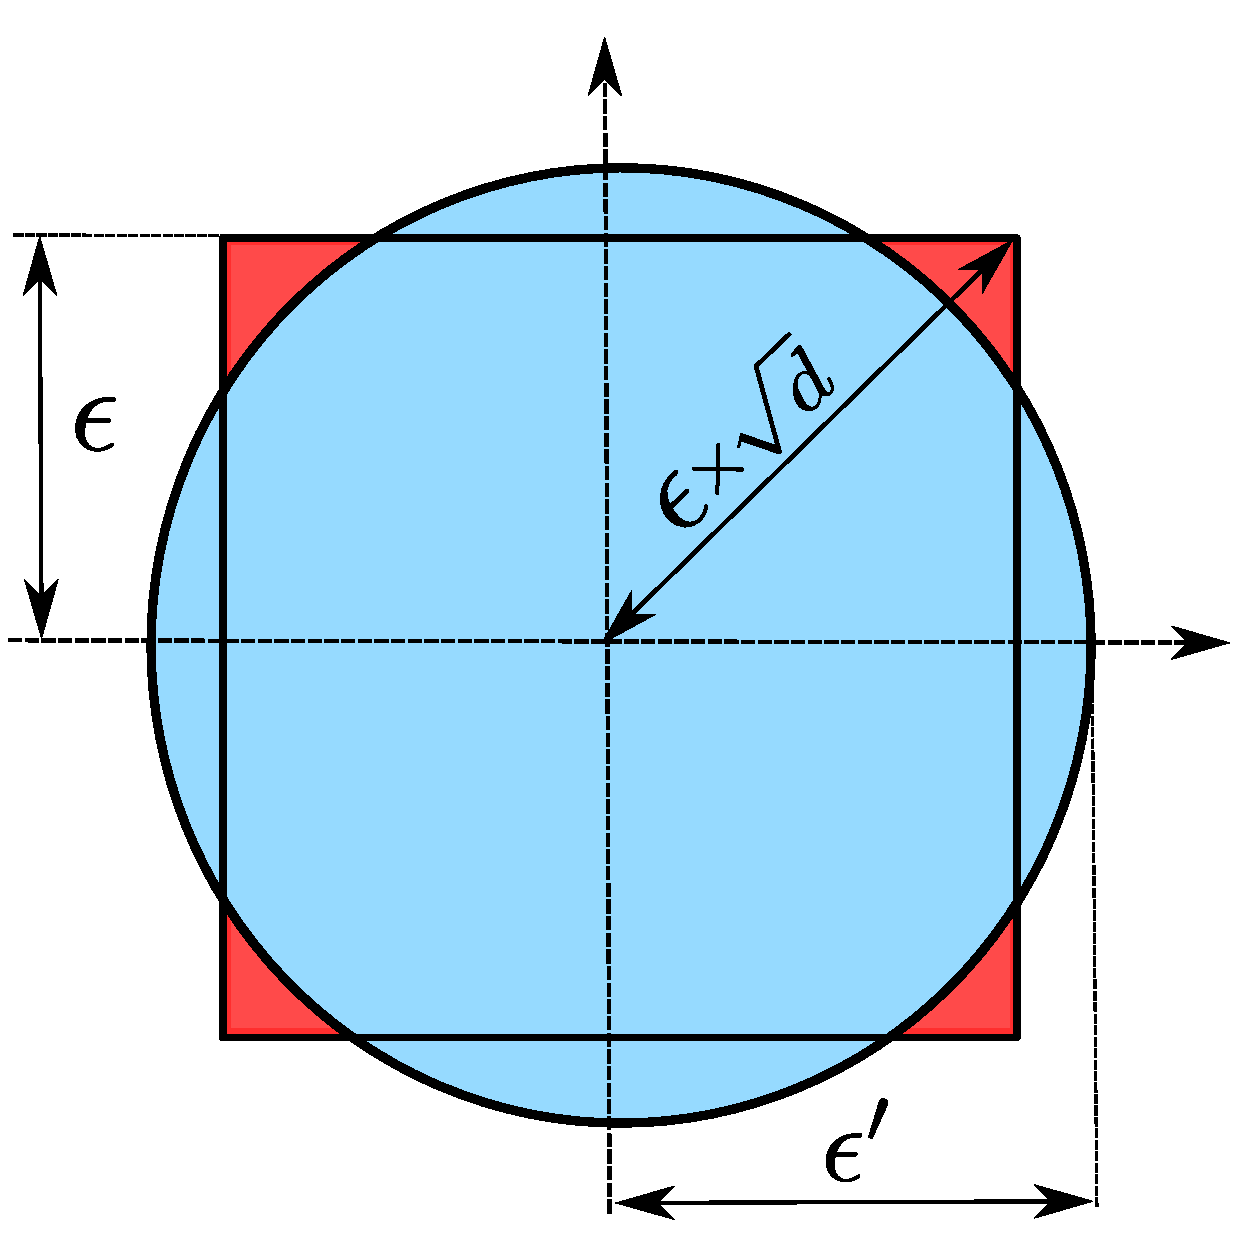
\includegraphics[scale=0.15]{sections/appendix/ecml_rat/graphs/BallInclusionAdversarialtraining2.pdf}\\(a)
  \end{minipage}
  \begin{minipage}{.32\linewidth}
    \centering
    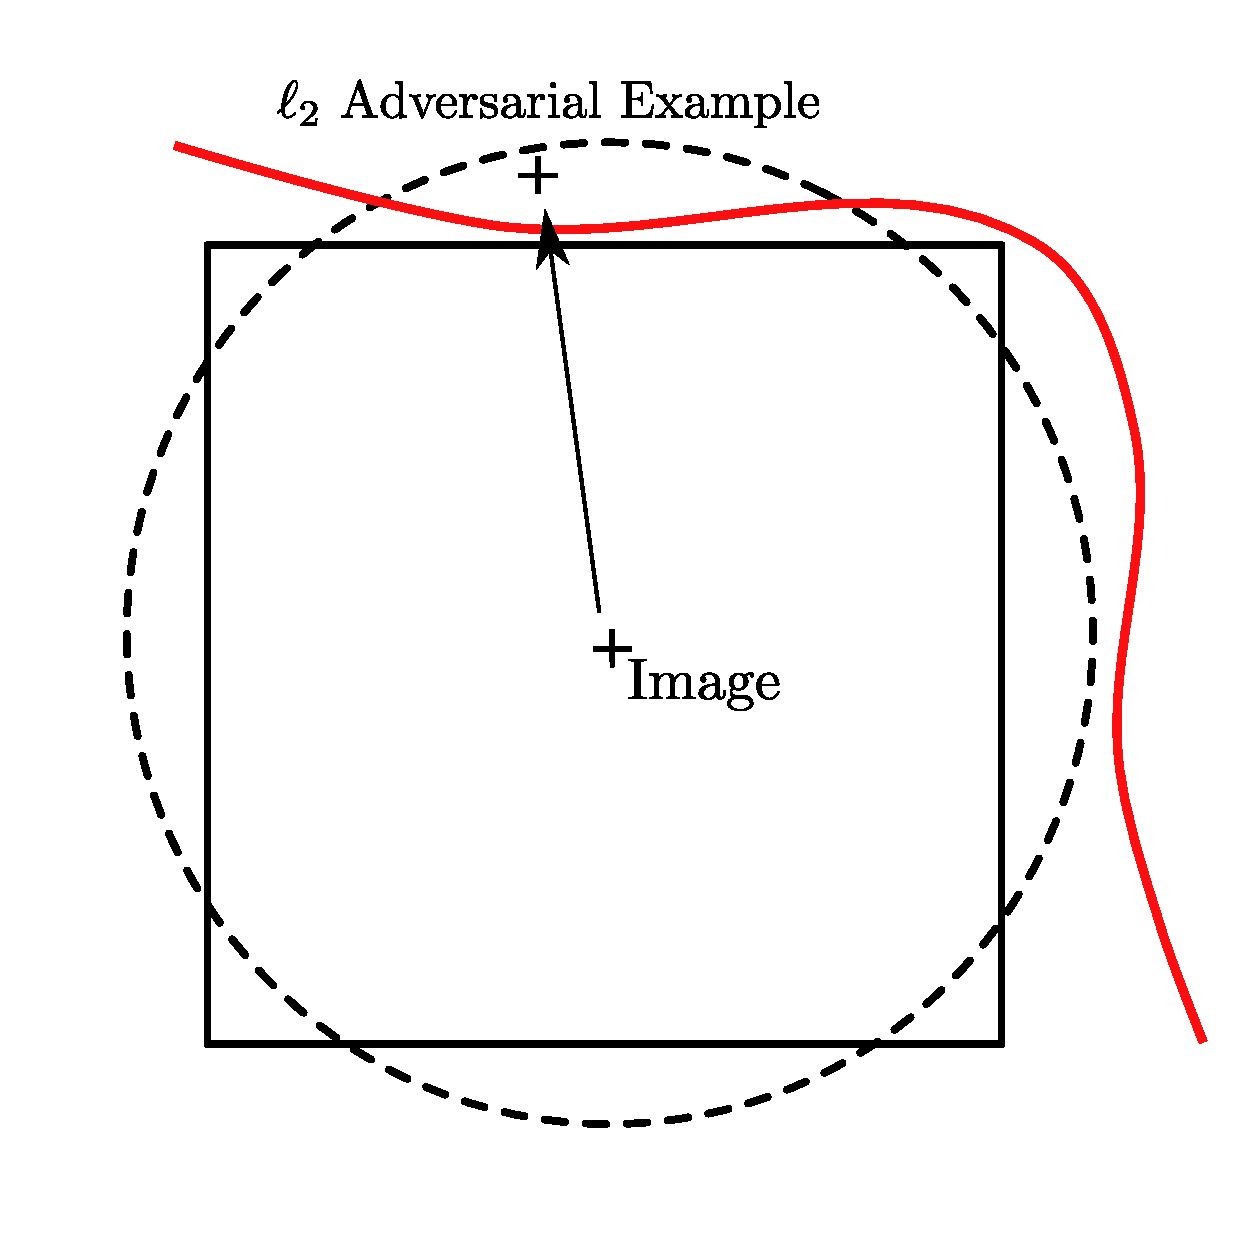
\includegraphics[scale=0.15]{sections/appendix/ecml_rat/graphs/BallAdversarialL2DecisionBoundary.pdf}\\(b)
  \end{minipage}
  \begin{minipage}{.32\linewidth}
      \centering
      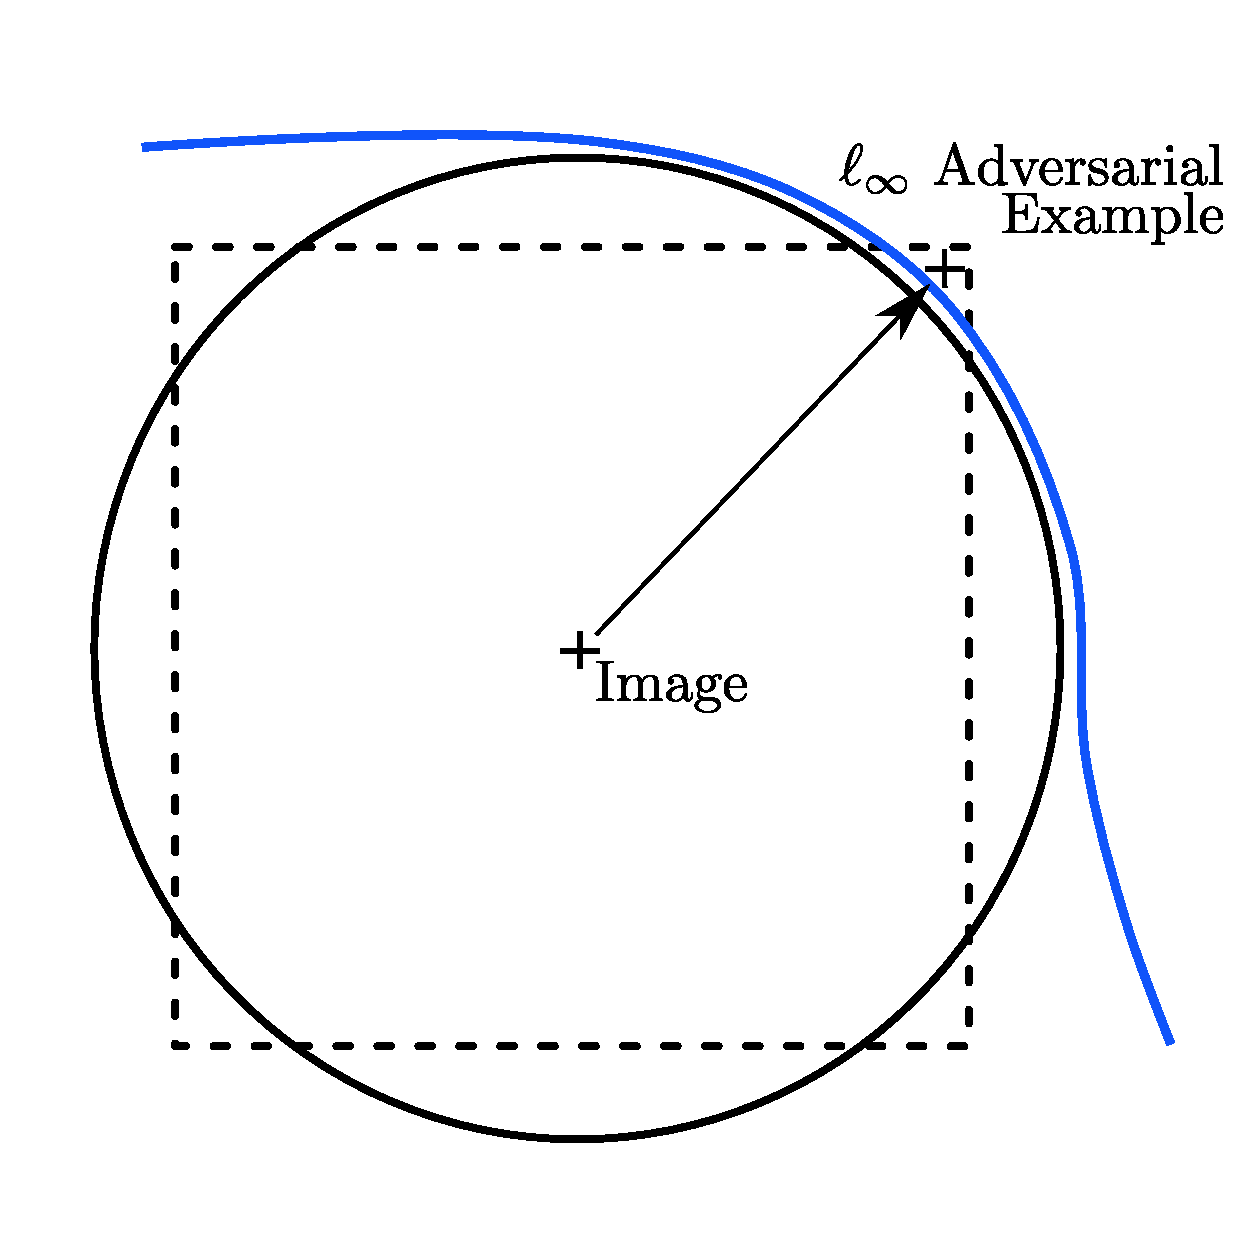
\includegraphics[scale=0.15]{sections/appendix/ecml_rat/graphs/BallAdversarialLinfDecisionBoundary.pdf}\\(c)
  \end{minipage}
    \caption{ Left: 2D representation of the $\ell_\infty$ and $\ell_2$ balls of respective radius $\epsilon$ and $\epsilon'$. 
    Middle: a classifier trained with $\ell_\infty$ adversarial perturbations  (materialized by the red line) remains vulnerable to $\ell_2$ attacks. 
    Right: a classifier trained with $\ell_2$ adversarial perturbations (materialized by the blue line) remains vulnerable to $\ell_\infty$ attacks.}
  \label{figure:balls}
\end{figure*}%

\subsection{Theoretical analysis}

Let us consider a classifier $f_{\infty}$ that is provably robust against adversarial examples with maximum $\ell_\infty$ norm of value $\epsilon_\infty$. It guarantees that for any input-output pair $(x,y) \sim \mathcal D$ and for any perturbation $\tau$ such that $\lVert\tau\rVert_\infty \leq \epsilon_\infty$, $f_{\infty}$ is not misled by the perturbation, \emph{i.e.}, $f_{\infty}(x + \tau) = f_{\infty}(x)$.
We now focus our study on the performance of this classifier against adversarial examples bounded with a $\ell_2$ norm of value $\epsilon_2$. Using Figure~\ref{figure:balls}(a), we observe that any $\ell_2$ adversarial example that is also in the $\ell_\infty$ ball, will not fool $f_{\infty}$. Conversely, if it is outside the ball, we have no guarantee.

To characterize the probability that such an  $\ell_2$ perturbation fools an $\ell_\infty$ defense mechanism in the general case (\emph{i.e.}, any dimension $d$), we measure the ratio between the volume of the intersection of the $\ell_\infty$ ball of radius $\epsilon_\infty$ and the $\ell_2$ ball of radius $\epsilon_2$. As Theorem~\ref{theorem:nullvolume} shows, this ratio depends on the dimensionality $d$ of the input vector $x$, and  rapidly converges to zero when $d$ increases. 
Therefore a defense mechanism that protects against all $\ell_\infty$ bounded adversarial examples is unlikely to be efficient against $\ell_2$ attacks. 


\begin{thm}[Probability of the intersection goes to $0$]
\label{theorem:nullvolume}
\noindent Let $B_{2,d}(\epsilon) :=\left \{\tau \in \mathbb{R}^d \text{ s.t } \lVert\tau\rVert_2 \leq  \epsilon \right \}$ and $B_{\infty,d}(\epsilon') :=\left \{\tau \in \mathbb{R}^d \text{ s.t } \lVert\tau\rVert_\infty \leq  \epsilon' \right\}$. If for all $d$, we select $\epsilon$ and $\epsilon$' such that $\Vol\left(B_{2,d}(\epsilon)\right) =\Vol\left(B_{\infty,d}(\epsilon')\right)$, then $$\frac{\Vol\left(B_{2,d}(\epsilon)\bigcap B_{\infty,d}(\epsilon')\right)}{\Vol\left(B_{\infty,d}(\epsilon')\right)} \rightarrow 0 \text{ when } d\rightarrow \infty. $$
\end{thm} 
\begin{proof} 
Without loss of generality, let us fix $\epsilon=1$. One can show that for all $d$, 
\begin{equation}
    \Vol\left( B_{2,d}\left(\frac{2}{\sqrt{\pi}}\Gamma\left(\frac{d}{2}+1\right)^{1/d}\right)\right) = \Vol\left(B_{\infty,d}\left(1\right)\right)
\end{equation}
where $\Gamma$ is the gamma function. Let us denote 
\begin{equation}
    r_2(d)=\frac{2}{\sqrt{\pi}}\Gamma\left(\frac{d}{2}+1\right)^{1/d}.
\end{equation}
Then, thanks to Stirling's formula
\begin{equation}
    r_2(d)\sim \sqrt{\frac{2}{\pi e}} d^{1/2}.
\end{equation}
Finally, if we denote $\mathcal{U}_S$, the uniform distribution on set $S$, by using  Hoeffding inequality between Equation~\ref{eq:Hoeffding1} and \ref{eq:Hoeffding2}, we get:
\begin{align}
&\frac{\Vol(B_{2,d}(r_2(d))\bigcap B_{\infty,d}(1))}{\Vol(B_{\infty,d}(1))} \\
=&\PP_{x\sim \mathcal{U}_{B_{\infty,d}(1)}}\left[x\in B_{2,d}(r_2(d))\right] \\
=&\PP_{x\sim \mathcal{U}_{B_{\infty,d}(1)}}\left[\textstyle \sum_{i=1}^d |x_i|^2\leq r_2^2(d)\right] \\
\leq &\exp{- d^{-1} \left( r_2^2(d)-d\mathbb{E}|x_1|^2\right)^2} \label{eq:Hoeffding1} \\
\leq &\exp{-\left( \frac{2}{\pi e}-\frac13\right)^2d+ o(d)} \label{eq:Hoeffding2}.
\end{align}
\noindent
Then the ratio between the volume of the intersection of the ball and the volume of the ball converges towards $0$ when $d$ goes to $\infty$.
\end{proof}

Theorem~\ref{theorem:nullvolume} states that, when $d$ is large enough, $\ell_2$ bounded perturbations have a null probability of being also in the $\ell_\infty$ ball of the same volume. As a consequence, for any value of $d$ that is large enough, a defense mechanism that offers full protection against $\ell_\infty$ adversarial examples is not guaranteed to offer any protection against $\ell_2$ attacks\footnote{Th. \ref{theorem:nullvolume} can easily be extended to any two balls with different norms. For clarity, we restrict to the case of $\ell_\infty$ and $\ell_2$ norms.}.

\begin{table}[ht]
\centering
\caption{ Bounds of Theorem~\ref{theorem:nullvolume} on the volume of the intersection of  $\ell_2$ and $\ell_\infty$ balls at equal volume for typical image classification datasets. When $d=2$, the bound is $ 10^{-0.009}\approx 0.98$.}
\begin{tabular}{c r r r l}
\toprule
\textbf{Dataset\ } & \phantom{....} & \textbf{Dim.} $\mathbf{(d)}$ & \phantom{....} & \textbf{Vol. of the intersection }\\
\midrule
-- & & 2\ \ & & $10^{-0.009}$ \quad ($\approx$ 0.98) \\
MNIST & & 784\ \  & & $10^{-144}$\\
CIFAR & & 3072\ \ & &  $10^{-578}$\\
ImageNet & & 150528\ \ & & $10^{-28946}$\\
\bottomrule
\end{tabular}
\label{table:datadim}
\end{table}

Note that this result defeats the 2-dimensional intuition: if we consider a 2 dimensional problem setting, the $\ell_\infty$ and the $\ell_2$ balls have an important overlap (as illustrated in Figure~\ref{figure:balls}(a)) and the probability of sampling at the intersection of the two balls is bounded by approximately 98\%. However, as we increase the dimensionality $d$, this probability quickly becomes negligible, even for very simple image datasets such as MNIST. An instantiation of  the bound for classical image datasets is presented in Table~\ref{table:datadim}. The probability of sampling at the intersection of the $\ell_\infty$ and $\ell_2$ balls is close to zero for any realistic image setting. In large dimensions, the volume of the corner of the $\ell_\infty$ ball is much bigger than it appears in Figure~\ref{figure:balls}(a).


\subsection{No Free Lunch in Practice}

Our theoretical analysis shows that if adversarial examples were uniformly distributed in a high-dimensional space, then any mechanism that perfectly defends against $\ell_\infty$ adversarial examples has a null probability of protecting against $\ell_2$-bounded adversarial attacks. Although existing defense mechanisms do not necessarily assume such a distribution of adversarial examples, we demonstrate that whatever distribution they use, it offers no favorable bias with respect to the result of Theorem~\ref{theorem:nullvolume}. 
As we discussed in Section~\ref{sec:preliminaries_rat}, there are two distinct attack settings: loss maximization (PGD) and perturbation minimization (C\&W). Our analysis is mainly focusing on loss maximization attacks. However, these attacks have a very strict geometry\footnote{Due to the projection operator, all PGD attacks saturate the constraint, which makes them all lies in a very small part of the ball.}. This is why, to present a deeper analysis of the behavior of adversarial attacks and defenses, we also present a set of experiments that use perturbation minimization attacks.

\begin{table}[htbp]
  \centering 
  \caption{Average norms of PGD-$\ell_2$ and PGD-$\ell_\infty$ adversarial examples with and without $\ell_\infty$ adversarial training on CIFAR-10 ($d=3072$).}
    \begin{tabular}{lrrrrrrrr}
    \toprule
      & \phantom{...}  & \multicolumn{3}{c}{Attack PGD-$\ell_2$} & \phantom{...}  & \multicolumn{3}{c}{Attack PGD-$\ell_\infty$} \\
\cmidrule{3-5}\cmidrule{7-9}      &   & \multicolumn{1}{l}{Unprotected} &  \phantom{...} & \multicolumn{1}{l}{AT-$\ell_\infty$} &   & \multicolumn{1}{l}{Unprotected} & \phantom{...}  & \multicolumn{1}{l}{AT-$\ell_2$} \\
    \midrule
    Average $\ell_2$ norm &   & 0.830 &   & 0.830 &   & 1.400 &   & 1.640 \\
    Average $\ell_\infty$ norm &   & 0.075 &   & 0.200 &   & 0.031 &   & 0.031 \\
    \bottomrule \\
    \end{tabular}%
  \label{tab:mean_norm_pgd_attack_ben}%
\end{table}%

\paragraph{Adversarial training vs. loss maximization attacks}

To demonstrate that $\ell_\infty$ adversarial training is not robust against PGD-$\ell_2$ attacks we measure the evolution of $\ell_2$ norm of adversarial examples generated with PGD-$\ell_\infty$ between an unprotected model and a model trained with AT-$\ell_\infty$, \emph{i.e.}, AT where adversarial examples are generated with PGD-$\ell_\infty$ \footnote{To do so, we use the same experimental setting as in Section~\ref{sec:building_defense_mechanisms} with $\epsilon_\infty$ and $\epsilon_2$ such that the volumes of the two balls are equal.}. 
Results are presented in  Table~\ref{tab:mean_norm_pgd_attack_ben}. \footnote{All experiments in this section are conducted on CIFAR-10, and the experimental setting is fully detailed in Section~\ref{sec:experimental_settings}. }

The analysis is unambiguous: the average $\ell_\infty$ norm of a bounded $\ell_2$ perturbation more than double between an unprotected model and a model trained with AT PGD-$\ell_\infty$. This phenomenon perfectly reflects the illustration of Figure~\ref{figure:balls} (c). The attack will generate an adversarial example on the corner of the $\ell_\infty$ ball thus increasing the $\ell_\infty$ norm while maintaining the same $\ell_2$ norm. 
We can observe the same phenomenon with AT-$\ell_2$ against PGD-$\ell_\infty$ attack (see Figure~\ref{figure:balls} (b) and Table \ref{tab:mean_norm_pgd_attack_ben}). PGD-$\ell_\infty$ attack increases the $\ell_2$ norm while maintaining the same $\ell_\infty$ perturbation thus generating the perturbation in the upper area. 

As a consequence, we cannot expect adversarial training $\ell_\infty$ to offer any guaranteed protection against $\ell_2$ adversarial examples .

\paragraph{Adversarial training vs. perturbation minimization attacks.}
To better capture the behavior of $\ell_2$ adversarial examples, we now study the performances of an $\ell_2$ perturbation minimization attack (C\&W) with and without AT-$\ell_\infty$. It allows us to understand in which area C\&W discovers adversarial examples and the impact of AT-$\ell_\infty$. In high dimensions, the red corners (see Figure~\ref{figure:balls} (a)) are very far away from the $\ell_2$ ball. Therefore, we hypothesize that a large proportion of the $\ell_2$ adversarial examples will remain unprotected. To validate this assumption, we measure the proportion of adversarial examples inside of the $\ell_2$ ball before and after $\ell_\infty$ adversarial training. The results are presented in Figure~\ref{fig:calotte} (left: without adversarial training, right: with adversarial training). 

\begin{figure}[htb]
    \centering
    \begin{tikzpicture}[scale=0.5]
    \begin{groupplot}[group style={
                        group name=myplot,
                        group size= 2 by 1},
                        grid style=dashed,
                        ymajorgrids=true]
       
    \nextgroupplot[stack plots=y,area style,ytick={0,5000,1000},ymin=0,ymax=10000,xmin=0.3,xmax=16.63,axis x line*=bottom, axis y line*=left,xtick={2,14},xticklabels={\Large $\epsilon'=\epsilon\phantom{\sqrt{d}}$, \Large $\epsilon'=\epsilon\times\sqrt{d}$},xtick style={draw=none}]
        \addplot table [x=eps,y=linf_ball] {sections/appendix/ecml_rat/graphs/data/ball_l2_base.dat}\closedcycle;
        \addplot table [x=eps,y=callote] {sections/appendix/ecml_rat/graphs/data/ball_l2_base.dat}\closedcycle;
        \addplot table [x=eps,y=outside] {sections/appendix/ecml_rat/graphs/data/ball_l2_base.dat}\closedcycle;

    \nextgroupplot[stack plots=y,area style,ytick={0,5000,1000},ymin=0,ymax=10000,xmin=0.3,xmax=16.63,axis x line*=bottom, axis y line*=left,xtick={2,14},xticklabels={\Large $\epsilon'=\epsilon\phantom{\sqrt{d}}$, \Large $\epsilon'=\epsilon\times\sqrt{d}$},xtick style={draw=none}]
        \addplot table [x=eps,y=linf_ball] {sections/appendix/ecml_rat/graphs/data/ball_l2_at.dat}\closedcycle;
        \addplot table [x=eps,y=callote] {sections/appendix/ecml_rat/graphs/data/ball_l2_at.dat}\closedcycle;
        \addplot table [x=eps,y=outside] {sections/appendix/ecml_rat/graphs/data/ball_l2_at.dat}\closedcycle;

    \end{groupplot}
% \matrix[
%     matrix of nodes,
%     anchor=north,
%     inner sep=0.2em,
%   ]at(11,-1.5)
%   {
%     \ref{plots:plot1} & \small R.N.\cite{pinot2019theoretical} & [5pt]
%     \ref{plots:plot2} & \small RAT (our approach) & [5pt]
%     \ref{plots:plot3} & \small LeRAT (our approach)\\};
\end{tikzpicture}

%%% Local Variables:
%%% mode: latex
%%% TeX-master: t
%%% End:

    \caption{Comparison of the number of adversarial examples found by C\&W, inside the $\ell_\infty$ ball (lower, blue area), outside the $\ell_\infty$ ball but inside the $\ell_2$ ball (middle, red area) and outside the $\ell_2$ ball (upper gray area). $\epsilon$ is set to $0.3$ and $\epsilon'$ varies along the x-axis. Left: without adversarial training, right: with adversarial training. Most adversarial examples have shifted from the $\ell_\infty$ ball to the cap of the $\ell_2$ ball, but remain at the same $\ell_2$ distance from the original example.}
    \label{fig:calotte}
\end{figure}

On both charts, the blue area represents the proportion of adversarial examples that are inside the $\ell_\infty$ ball. The red area represents the adversarial examples that are outside the $\ell_\infty$ ball but still inside the $\ell_2$ ball (valid $\ell_2$ adversarial examples). Finally, the brown-beige area represents the adversarial examples that are beyond the $\ell_2$ bound. The radius $\epsilon'$ of the $\ell_2$ ball varies along the x-axis from $\epsilon'$ to $\epsilon' \sqrt{d}$. On the left chart (without adversarial training) most $\ell_2$ adversarial examples generated by C\&W are inside both balls. On the right chart most of the adversarial examples have been shifted out the $\ell_\infty$ ball. This is the expected consequence of $\ell_\infty$ adversarial training. However, these adversarial examples remain in the $\ell_2$ ball, \emph{i.e.}, they are in the cap of the $\ell_2$ ball. These examples are equally good from the $\ell_2$ perspective. This means that even after adversarial training, it is still easy to find good $\ell_2$ adversarial examples, making the $\ell_2$ robustness of AT-$\ell_\infty$ almost null. 


\section{Reviewing Defenses Against Multiple Attacks}
\label{sec:building_defense_mechanisms}

\begin{table}[htbp]
  \centering
  \caption{This table shows a comprehensive list of results consisting of the accuracy of several defense mechanisms against $\ell_2$ and $\ell_\infty$ attacks. This table main objective is to compare the overall performance of ‘single‘ norm defense mechanisms (AT and NI presented in the Section~\ref{subsec:defense_mechanisms}) against mixed norms defense mechanisms (MAT \& RAT mixed defenses presented in Section~\ref{sec:building_defense_mechanisms}).}
    \begin{tabular}{lccccccccccccccccc}
    \toprule
      &   & \textbf{Baseline} & \phantom{...}  & \multicolumn{2}{c}{\textbf{AT}} & \phantom{...}  & \multicolumn{2}{c}{\textbf{MAT}} &  \phantom{...} & \multicolumn{2}{c}{\textbf{NI}} &  \phantom{...} & \multicolumn{2}{c}{\textbf{RAT}-$\ell_\infty$} &  \phantom{...} & \multicolumn{2}{c}{\textbf{RAT}-$\ell_2$} \\
\cmidrule{3-3}\cmidrule{5-6}\cmidrule{8-9}\cmidrule{11-12}\cmidrule{14-15}\cmidrule{17-18}      &   & -- &   & $\ell_\infty$ & $\ell_2$ &   & Max & Rand &   & $\mathcal{N}$ & $\mathcal{U}$ &   & $\mathcal{N}$ & $\mathcal{U}$ &   & $\mathcal{N}$ & $\mathcal{U}$ \\
    \midrule
    Natural &   & 0.94 &   & 0.85 & 0.85 &   & 0.80 & 0.80 &   & 0.79 & 0.87 &   & 0.74 & 0.80 &   & 0.79 & 0.87 \\
    PGD-$\ell_\infty$ &   & 0.00 &   & 0.43 & 0.37 &   & 0.37 & 0.40 &   & 0.23 & 0.22 &   & 0.35 & 0.40 &   & 0.23 & 0.22 \\
    PGD-$\ell_2$ &   & 0.00 &   & 0.37 & 0.52 &   & 0.50 & 0.55 &   & 0.34 & 0.36 &   & 0.43 & 0.39 &   & 0.34 & 0.37 \\
    \bottomrule
    \end{tabular}%
  \label{tab:results}
\end{table}%

Adversarial attacks have been an active topic in the machine learning community since their discovery~\cite{globerson2006nightmare, biggio2013evasion,Szegedy2013IntriguingPO}. Many attacks have been developed. Most of them solve a loss maximization problem with either $\ell_\infty$~\cite{goodfellow2014explaining,kurakin2016adversarial,madry2018towards}, $\ell_2$~\cite{carlini2017towards,kurakin2016adversarial,madry2018towards}, $\ell_1$~\cite{tramer2019adversarial} or $\ell_0$~\cite{papernot} surrogate norms. As we showed, these norms are really different in high dimension. Hence, defending against one norm-based attack is not sufficient to protect against another one. 
In order to solve this problem, we review several strategies to build defenses against multiple adversarial attacks. These strategies are based on the idea that both types of defense must be used simultaneously in order for the classifier to be protected against multiple attacks. The detailed description of the experimental setting is described in Section~\ref{sec:experimental_settings}. 



\subsection{Experimental Setting}
\label{sec:experimental_settings}

To compare the robustness provided by the different defense mechanisms, we use strong adversarial attacks and a conservative setting: the attacker has a total knowledge of the parameters of the model (white-box setting) and we only consider untargeted attacks  (a misclassification from one target to any other will be considered as adversarial). To evaluate defenses based on Noise Injection, we use {\em Expectation Over Transformation} (EOT), the rigorous experimental protocol  proposed by \cite{athalye2017synthesizing} and later used by \cite{athalye2018obfuscated,carlini2019evaluating} to identify flawed defense mechanisms. 

To attack the models, we use state-of-the-art algorithms PGD. We run PGD with 20 iterations to generate adversarial examples and with 10 iterations when it is used for adversarial training. The maximum $\ell_\infty$ bound is fixed to $0.031$ and the maximum $\ell_2$ bound is fixed to $0.83$. As discussed in Section~\ref{sec:preliminaries_rat}, we chose these values so that the $\ell_\infty$ and the $\ell_2$ balls have similar volumes. Note that $0.83$ is slightly above the values typically used in previous publications in the area, meaning the attacks are stronger, and thus  more difficult to defend against.

All experiments are conducted on CIFAR-10 with the Wide-Resnet 28-10 architecture. We use the training procedure and the hyper-parameters described in the original paper by~\cite{ZagoruykoK16}. Training time varies from 1 day (AT) to 2 days (MAT) on 4 GPUs-V100 servers. 


\subsection{MAT -- Mixed Adversarial Training}\label{subsec:mixed_adversarial_training}
Earlier results have shown that AT-$\ell_p$ improves the robustness against corresponding $\ell_p$-bounded adversarial examples, and the experiments we present in this section corroborate this observation (See Table~\ref{tab:results}, column: AT). Building on this, it is natural to examine the efficiency of \emph{Mixed Adversarial Training} (MAT) against mixed $\ell_\infty$ and $\ell_2$ attacks. MAT is a variation of AT that uses both $\ell_\infty$-bounded adversarial examples and $\ell_2$-bounded adversarial examples as training examples. As discussed in~\cite{tramer2019adversarial}, there are several possible strategies to mix the adversarial training examples. The first strategy (MAT-Rand) consists in randomly selecting one adversarial example among the two most damaging $\ell_\infty$ and $\ell_2$, and to use it as a training example, as described in Equation~(\ref{eq:mat-rand}): 
\paragraph{MAT-Rand}:
\begin{equation}
    \min_{\theta}\mathbb{E}_{(x, y) \sim \mathcal{D}} \left[\mathbb{E}_{p\sim\mathcal{U}({\{2, \infty\})}} \max_{\lVert\tau\rVert_p \leq \epsilon} \mathcal{L} \left( f_{\theta}(x+\tau), y \right) \right].
    \label{eq:mat-rand}
\end{equation}

\noindent
An alternative strategy is to systematically train the model with the most damaging adversarial example ($\ell_\infty$ or $\ell_2$). As described in Equation~(\ref{eq:mat-max}): 

\paragraph{MAT-Max}:
\begin{equation}
    \min_{\theta}\mathbb{E}_{(x, y) \sim \mathcal{D}} \left[ \max_{p \in \{2, \infty\}} \max_{\lVert\tau\rVert_p \leq \epsilon} \mathcal{L} \left( f_{\theta}(x+\tau), y \right) \right].
    \label{eq:mat-max}
\end{equation}

\noindent
The accuracy of MAT-Rand and MAT-Max are reported in Table~\ref{tab:results} (Column: MAT). As expected, we observe that MAT-Rand and MAT-Max offer better robustness both against PGD-$\ell_2$ and PGD-$\ell_\infty$ adversarial examples than the original AT does. More  generally, we can see that AT is a good strategy against loss maximization attacks, and thus it is not surprising that MAT is a good strategy against mixed loss maximization attacks. However efficient in practice, MAT (for the same reasons as AT) lacks theoretical arguments. In order to get the best of both worlds, \cite{salman2019provably} proposed to mix adversarial training with randomization.  


\subsection{RAT -- Randomized Adversarial Training}\label{subsec:randomized_adversarial_training}

We now examine the performance of Randomized Adversarial Training (RAT) first introduced in~\cite{salman2019provably}. This technique mixes Adversarial Training with Noise Injection. The corresponding loss function is defined as follows: \begin{equation}
    \min_{\theta}\mathbb{E}{(x, y) \sim \mathcal{D}} \left[ \max_{\lVert\tau\rVert_p \leq \epsilon} \mathcal{L} \left( \tilde{f}_{\theta}(x+\tau), y)  \right) \right].
\end{equation}
\noindent where $\tilde{f}_\theta$ is a randomized neural network with noise injection as described in Section~\ref{subsec:randomized_training}, and $\lVert\cdot\rVert_p$ define which kind of AT is used. For each setting, we consider two noise distributions, Gaussian and Uniform as we did with NI. We also consider two different Adversarial training AT-$\ell_\infty$ as well as AT-$\ell_2$. 

The results of RAT are reported in Table~\ref{tab:results}~(Columns: RAT-$\ell_\infty$ and RAT-$\ell_2$).
We can observe that RAT-$\ell_\infty$ offers the best extra robustness with both noises, which is consistent with previous experiments, since AT is generally more effective against $\ell_\infty$ attacks whereas NI is more effective against $\ell_2$-attacks. Overall, RAT-$\ell_\infty$ and a noise from uniform distribution offers the best performances but is still weaker than MAT-Rand.
These results are also consistent with the literature, since adversarial training (and its variants) is the best defense against adversarial examples so far.


\section{Conclusion \& Perspective}
In this paper, we tackled the problem of protecting neural networks against multiple attacks crafted from different norms. We demonstrated and gave a geometrical interpretation to explain why most defense mechanisms can only protect against one type of attack. Then we reviewed existing strategies that mix defense mechanisms in order to build models that are robust against multiple adversarial attacks. We conduct a rigorous and full comparison of {\em Randomized Adversarial Training} and {\em Mixed Adversarial Training} as defenses against multiple attacks. 

We could argue that both techniques offer benefits and limitations. We have observed that MAT offers the best empirical robustness against multiples adversarial attacks but this technique is computationally expensive which hinders its use in large-scale applications. Randomized techniques have the important advantage of providing theoretical guarantees of robustness and being computationally cheaper. However, the certificate provided by such defenses is still too small for strong attacks. Furthermore, certain Randomized defenses also suffer from the curse of dimensionality as recently shown by \cite{kumar2020curse}. 

Although, randomized defenses based on noise injection seem limited in terms of accuracy under attack and scalability, they could be improved either by Learning the best distribution to use or by leveraging different types of randomization such as discrete randomization first proposed in \cite{pinot2020randomization}. We believe that these certified defenses are the best solution to ensure the robustness of classifiers deployed into real-world applications. 




    
    

\chapter{Adversarial Attacks on Linear Contextual Bandits}
\label{paper:banditsattacks}
\newcommand{\mtb}[1]{\textcolor{black}{#1}}
\newcommand{\otc}[1]{\textcolor{black}{#1}}
\newcommand{\changede}[1]{\textcolor{black}{#1}}
\newcommand{\changebr}[1]{\textcolor{black}{#1}}
\newcommand{\changelm}[1]{\textcolor{black}{#1}}
\newcommand{\changebrtwo}[1]{\textcolor{black}{#1}}
\newcommand{\changee}[1]{\textcolor{black}{#1}}
\newcommand{\cmmnt}[1]{\ignorespaces}


\begin{abstract}
Contextual bandit algorithms are applied in a wide range of domains, from advertising to recommender systems, from clinical trials to education. In many of these domains, malicious agents may have incentives to {force a bandit algorithm into a desired behavior.} %attack the bandit algorithm to induce it to perform a desired behavior.
For instance, an unscrupulous ad publisher may try to increase their own revenue at the expense of the advertisers; a seller may want to increase the exposure of their products, or thwart a competitor's advertising campaign.
In this paper, we study several attack scenarios and show that a malicious agent can force a linear contextual bandit algorithm to pull any desired arm $T - o(T)$ times over a horizon of $T$ steps, while applying adversarial modifications to either rewards or contexts {with a cumulative cost} that only grow logarithmically as $O(\log T)$.
We also investigate the case when a malicious agent is interested in affecting the behavior of the bandit algorithm in a single context (e.g., a specific user). We first provide sufficient conditions for the feasibility of the attack and %we then propose 
an efficient algorithm to perform an attack. %test
{We empirically validate the proposed approaches in synthetic and real-world datasets.} %o  ur theoretical results on experiments performed on both synthetic and real-world datasets.
\end{abstract}





% !TEX root = main.tex
\section{Introduction}

% \todol{split the intro in two parts or make subtitles}

Recommender systems are at the heart of the business model of many industries like e-commerce or video streaming~\cite{davidson2010youtube,gomez2015netflix}. The two most common approaches for this task are based either on matrix factorization \cite{park2017comparative} or bandit algorithms \cite{li2010contextual}, which both
rely on a unaltered feedback loop between the recommender system and the user. In recent years, a fair amount of work has been dedicated to understanding how targeted perturbations in the feedback loop can fool a recommender system into recommending low quality items.

Following the line of research on adversarial attacks in supervised learning \cite{biggio2012poisoning,goodfellow2014explaining, jagielski2018manipulating, li2016data, liu2017robust}, attacks on recommender systems have been focused on filtering-based algorithms \cite{10.1145/3298689.3347031, mehta2008attack} and offline contextual bandits \cite{ma2018data}.
 % studying the effects of poisoning a dataset used by a learning algorithm. For recommender systems, those works are related to the study of attacks on Collaborative
The question of adversarial attacks for online bandit algorithms %(that is to say learning on the fly and not in batch)
has only \cmmnt{started being} \changee{been studied} quite recently \cite{jun2018adversarial, liu2019data, Immorlica2018AdversarialBW, guan2020robust}, and solely in the multi-armed stochastic setting.
Although the idea of online adversarial bandit algorithms is not new (see \expthree algorithm in \cite{auer2002finite}), the focus is different from what we are considering \changee{in this article}. Indeed, algorithms like \expthree or \expfour \cite{lattimore2018bandit} are designed to find optimal actions in hindsight in order to adapt to any rewards stream\cmmnt{ without any further assumptions}. 


 The opposition between adversarial and stochastic bandit settings has sparked interests in studying a middle ground.
 In \cite{bubeck2012best}, the learning algorithm has no knowledge of the type of feedback it receives \changee{(either stochastic or adversarial)}. In \cite{lykouris2018stochastic, li2019stochastic, gupta2019better, Lykouris2019CorruptionRE, kapoor2019corruption}, the rewards are assumed to be \changee{corrupted by adversarial rewards}\cmmnt{ but can be perturbed by some attacks}. The authors focus on \changee{building} algorithms able to find the optimal actions even in the presence of some non-random perturbations. \changee{This setting is different from what is studied in this article because} those perturbations are bounded and agnostic to \changee{arms pulled} by the learning algorithm, \changee{i.e., the adversary corrupt the rewards before the algorithm chooses an arm.}

% In addition, the opposition between the adversarial bandit setting and the stochastic setting %more classical one where the eward are assumed to be drawn from a stationary random distribution
% has sparked interests in studying a middle ground where the learning algorithm
% has no knowledge of the type of feedback it receives \citep[e.g.,][]{bubeck2012best} and %However, the recent growth in the use of bandit algorithms has
% % shown that the stochastic assumption is mostly true (up to some uncontrolled perturbations) in an overwhelming number of cases, the study of this setting where
% where rewards are assumed to be stochastic but can be perturbed by some attacks %has given birth to a very recent line of work
% \cite{li2019stochastic, gupta2019better, Lykouris2019CorruptionRE, kapoor2019corruption}. \changede{Those last works being focused} on constructing algorithms able to find the optimal actions even in the presence of some non-reward perturbations but bounded and agnostic to the choices of the learning algorithm.
% \todot{Previous sentence is not clear. You are referring to second work not ``best of both worlds'', right?}
In the broader Deep Reinforcement Learning (DRL) literature, the focus is placed on modifying the observations of different states to fool a DRL system at inference time
\cite{hussenot2019targeted, sunstealthy} \changee{or the rewards \cite{ma2019policy}.}
\paragraph{Contribution.}In this work, we first follow the research direction opened by \cite{jun2018adversarial} where the attacker has the objective of fooling a learning algorithm into taking a specific action as much as possible. \changee{For example} \cmmnt{Consider } in a news recommendation problem, as described in \cite{li2010contextual}, a bandit algorithm chooses between $K$ articles to recommend to a user, based on some information about them, \changee{called} context. We assume that an attacker sits between the user and the website, they can choose the reward (i.e., click or not) for the recommended article observed by the recommending algorithm. Their goal is to fool the bandit algorithm into recommending \changee{some articles} \cmmnt{\changelm{a particular or a set of target articles}} to most users. The contributions of our work can be summarized as follows:
\begin{itemize}
    \item We extend the work of~\cite{jun2018adversarial, liu2019data} to the contextual linear bandit setting showing how to perturb rewards for both stochastic and adversarial algorithms, forcing \textbf{any} bandit algorithms to pull a specific set of arms, $o(T)$ times for logarithmic cost for the attacker.
    \item We analyze, for the first time, the setting in which the attacker can only modify the context $x$ associated with the current user (the reward is not altered). The goal of the attacker is to fool the bandit algorithm into pulling arms of a target set for most users (\ie contexts) while minimizing the total norm of their attacks. We show that the widely known \linucb algorithm \cite{abbasi2011improved, lattimore2018bandit} is vulnerable to this new type of attack.
    \item We present a harder setting for the attacker, where the latter can only modify the context associated to a specific user. This situation may occur when a malicious agent has infected some computers with a Remote Access Trojan (RAT). The attacker can then modify the history of navigation of a specific user and, as a consequence, the information seen by the online recommender system.We show how the attacker can attack the two very common bandit algorithms \linucb and Linear Thompson Sampling (\lints) \cite{agrawal2013thompson,abeille2017linear} and, in certain cases, force them to pull a set of arms most of the time \changebr{when} a specific context (\ie user) is presented to the algorithm (\ie visits a website). 
\end{itemize}




% !TEX root = main.tex
\section{Preliminaries}\label{sec:preliminaries}
We consider the standard contextual linear bandit setting with $K\in \mathbb{N}$ arms. At each time $t$, the agent observes a context $x_{t}\in\mathbb{R}^{d}$, selects an action $a_{t}\in \llbracket 1, K\rrbracket$ and observes a reward: $r_{t,a_{t}} = \langle \theta_{a_{t}}, x_{t}\rangle + \eta_{a_{t}}^{t}$ where for each arm $a$, $\theta_{a}\in \mathbb{R}^{d}$ is a feature vector and $\eta_{a_{t}}^{t}$ is a conditionally independent zero-mean, $\sigma^{2}$-subgaussian noise.  \changee{The contexts are assumed to be sampled \textit{stochastically} except in App.~\ref{app:adversarial_rewards}.} \cmmnt{We also make the following assumptions on the contexts and parameter vectors.}
\begin{assump}\label{assumption1}
There exist $L>0$ and $\mathcal{D}\subset \mathbb{R}^{d}$, such that for all $t$, $x_{t}\in\mathcal{D}$ and, $\forall x\in\mathcal{D},\forall a\in\llbracket 1, K\rrbracket,~ \|x\|_{2} \leq L \text{ and } \langle \theta_{a}, x\rangle \in (0,1]$. In addition, we assume that there exists $S>0$ such that $\|\theta_{a}\|_{2}\leq S$ for all arms $a$.
\end{assump}
The agent minimizes the cumulative regret after $T$ steps $R_{T} = \sum_{t=1}^{T} \langle \theta_{a^{\star}_{t}}, x_{t}\rangle - \langle \theta_{a_{t}}, x_{t}\rangle$,
where $a_{t}^{\star} := \argmaxB_{a} \langle \theta_{a}, x_{t}\rangle$.
A bandit learning algorithm $\mathfrak{A}$ is said to be \emph{no-regret} when it satisfies $R_{T} = o(T)$, i.e., the average expected reward received by $\mathfrak{A}$ \changebr{converges} to the optimal one. Classical bandit algorithms (\eg \linucb and \lints) compute an estimate of the unknown parameters $\theta_a$ using past observations. Formally, for each arm $a \in [K]$ we define $S_a^t$ as the set of times up to $t-1$ (included) where the agent played arm $a$. Then, the estimated parameters are obtained through regularized least-squares regression as $\wh{\theta}_a^t = (X_{t,a} X_{t,a}^\top + \lambda I)^{-1} X_{t,a} Y_{t,a}$, where $\lambda > 0$, $X_{t,a} = (x_i)_{i \in S_a^t} \in \mathbb{R}^{d \times |S_a^t|}$ and $Y_{t,a} = (r_{i,a_i})_{i \in S_a^t} \in \mathbb{R}^{|S_a^t|}$.
Denote by $V_{t,a} = \lambda I + X_{t,a} X_{t,a}^\top$ the design matrix of the regularized least-square problem and by $\|x\|_{V} = \sqrt{x^\top V x}$ the weighted norm \wrt any positive matrix $V \in \mathbb{R}^{d \times d}$.
We define the confidence set:
\begin{equation}
\label{eq:confidence.intervals}
\mathcal{C}_{t,a} = \Big\{ \theta \in \mathbb{R}^d \,:\, \big\|\theta - \widehat{\theta}_{t,a} \big\|_{V_{t,a}} \leq \beta_{t,a} \Big\}
\end{equation}
% \begin{equation}
%         \label{eq:confidence.intervals}
%         \mathcal{C}_{t,a} = \left\{ \theta \in \mathbb{R}^d \,:\, \left\|\theta - \widehat{\theta}_{t,a} \right\|_{V_{t,a}} \leq \beta_{t,a} \right\}
% \end{equation}
 where 
%\begin{equation}
%\label{eq:beta_linucb}
        $\beta_{t,a} = \sigma\sqrt{d\log\big( (1 + L^2(1+|S_a^t|)/\lambda)/\delta \big)} + S\sqrt{\lambda},$
%\end{equation}
which guarantees that $\theta_{a}\in \mathcal{C}_{t,a}$, for all $t>0$, w.p.\ $1-\delta$.
%
This uncertainty is used to balance the exploration-exploitation trade-off either through optimism (\eg \linucb) or through randomization (\eg \lints). 



% \todot{add the confidence set property here}
% In this paper, we consider the case where a learning algorithm $\mathfrak{A}$ is attacked by an adversary that can modify different quantities in the learning process, like the rewards or the contexts observed by $\mathfrak{A}$. Similarly to \cite{liu2019data,jun2018adversarial} the goal of the attacker being to fool $\mathfrak{A}$ into pulling a target arm $a^{\dagger}$  $(T - o(T))$-times while maintaining the total number of modifications (i.e., cost) to be sub-linear. 



% !TEX root = main.tex
\section{Online Adversarial Attacks on Rewards}\label{sec:attacks_rewards}
The ultimate goal of a malicious agent is to force a bandit algorithm to perform a desired behavior. An attacker may simply want to induce the bandit algorithm to perform poorly\textemdash ruining the users' experience\textemdash or to force the algorithm to suggest a specific arm. The latter case is particularly interesting in advertising where a seller may want to increase the exposure of its product at the expense of the competitors. Note that the users' experience is also compromised by the latter attack since \changebr{ the suggestions they will receive will not be} tailored to their needs.
Similarly to~\cite{liu2019data,jun2018adversarial}, we focus on the latter objective, \ie to fool the bandit algorithm into pulling arms \changelm{ in $A^\dagger$, a set of target arms,} for $T-o(T)$ time steps (\emph{independently of the user}).

A way to obtain this behavior is to dynamically modify the reward in order to make the bandit algorithm believe that $a^\dagger$ is optimal, \changelm{for some $a^\dagger\in A^\dagger$.}
Clearly, the attacker has to pay a price in order to modify the perceived bandit problem and fool the algorithm.
If there is no restriction on when and how the attacker can alter the reward, the attacker can easily fool the algorithm.
However, this setting is not interesting since the attacker may pay a cost higher than the loss suffered by the attacked algorithm. An attack strategy is considered successful when the total cost of the attack is sublinear in $T$.
%\changebr{If there is no restriction on when and how they can attack, the attacker has complete control on the inputs of the bandit algorithm and can fool it easily. In practice, even though we restrict ourselves to attacking only the rewards or only the contexts,} we consider an attacker to be successful when the total cost of the attack is sublinear in $T$.%\todotout{explain better}

In this section, we show that under Assumption~\ref{assumption1}, there exists an attack algorithm that is successful against any bandit algorithm, stochastic or adverserial.

\textbf{Setting.} 
We assume that the attacker has the same knowledge as the bandit algorithm $\mathfrak{A}$ about the problem (\ie knows $\sigma$ and $L$). %\todotout{should know $L$ for $\beta$, right?}\todoeout{yes}
The attacker is assumed to be able to observe the context $x_t$, the arm $a_t$ pulled by $\mathfrak{A}$, and can modify the reward received by $\mathfrak{A}$.
When the attacker modifies the reward $r_{t, a_{t}}$ into $\wt{r}_{t, a_{t}}$ the \emph{instantaneous cost} of the attack is defined as $c_{t} :=\big| r_{t,a_{t}} - \wt{r}_{t, a_{t}}\big|$. The goal of the attacker is to fool algorithm $\mathfrak{A}$ such that \changelm{the arms in $A^\dagger$ are} pulled $T - o(T)$ times and $\sum_{t=1}^{T}  c_{t} = o(T)$. \changee{We also assume that the action for the arms in the target set is strictly positive for every context $x\in\mathcal{D}$. That is to say that $\Delta := \min_{x\in \mathcal{D}}\left\{ \langle x, \theta_{a_{\star}^{\dagger}(x)}\rangle - \max_{a\in A
^{\dagger}, a\neq a_{\star}^{\dagger}(x)} \langle x, \theta_{a}\rangle\right\}>0$ where $a_{\star}^{\dagger}(x) = \arg\max_{a\in A^{\dagger}} \langle x, \theta_{a}\rangle$ for every $x\in \mathcal{D}$}.


\textbf{Attack idea.} We leverage the idea presented in \cite{liu2019data} and \cite{jun2018adversarial} where the attacker lowers the reward of arms $a\notin A^{\dagger}$ so that algorithm $\mathfrak{A}$ learns that an arm of the target set is optimal for every context.
Since $\mathfrak{A}$ is assumed to be no-regret, the attacker only needs to modify the rewards $o(T)$ times to achieve this goal.
%As a consequence, the total cost of attacks is $o(T)$. 
%
Lowering the rewards has the effect of shifting
% Pushing down rewards consists in shifting  
the vectors $(\theta_{a})_{a\notin A^{\dagger}}$ to new vectors $(\theta'_{a})_{a\notin A^{\dagger}}$ such that for all arms $a\notin A^{\dagger}$ and all contexts $x\in\mathcal{D}$, there exists an arm $a^\dagger\in A^\dagger$  such that $\langle\theta'_{a}, x\rangle \leq \langle \theta_{a^{\dagger}}, x\rangle$. Since rewards are assumed to be bounded (see Asm.~\ref{assumption1}), this objective can be achieved by simply forcing the reward of non-target arms $a\notin A^\dagger$ to the minimum value.
Contextual ACE (see Fig.~\ref{alg:context_attack_protocol}) implements a soft version of this idea by leveraging the knowledge of the reward distribution.
At each round $t$, Contextual ACE modifies the reward perceived by $\mathfrak{A}$ as follows:
\vspace{-0.12cm}
 \begin{equation}
         \label{eq:perturbed.reward2}
 \widetilde{r}^{1}_{t,a_{t}} =\eta_{t}'\mathds{1}_{\{a_{t} \notin A^{\dagger}\}}+r_{t, a_t}\mathds{1}_{\{a_{t} \in A^{\dagger}\}} 
 \end{equation}
%  \begin{equation}
%          \label{eq:perturbed.reward2}
%  \widetilde{r}^{1}_{t,a_{t}} = \left\{\begin{matrix}
%  \eta_{t}'  & \text{if } a_{t} \neq a^{\dagger}\\ 
% 	 r_{t, a^{\dagger}} & \text{otherwise} 
% \end{matrix}\right.
%  \end{equation}

where $\eta_{t}'$ is a $\sigma$-subgaussian random variable generated by the attacker independently of all other random variables. Contextual ACE transforms the original problem into a \emph{stationary} bandit problem in which there is a targeted arm that is optimal for all contexts and all non targeted arms have expected reward of $0$. \changee{The following propostion shows that the cumulative cost of the attack is sublinear.}
%Despite this attack may seem expensive, the following proposition shows that its cumulative cost is sublinear.

% The approach used by the ACE algorithm \cite{liu2019data} effectively does this by constructing confidence intervals around the mean of each arm and feeding perturbed rewards to the bandit learner algorithm. However, the perturbed reward process seen by algorithm $\mathfrak{A}$ is non-stationary and in general there is no guarantee that an algorithm $\mathfrak{A}$ minimizing the regret in a stationary bandit problem keeps the same performance when the bandit problem is not stationary anymore. Nonetheless, transposing the idea of the ACE algorithm to our setting would give an attack of the following form, where at time $t$, Alg. $\mathfrak{A}$ pulls arm $a_{t}$ and receives rewards $\wt{r}^{1}_{t,a_{t}}$: 
% \begin{align*}
%         \wt{r}^{1}_{t, a_{t}} = \begin{cases}
%                 r_{t, a_{t}} + \max(-1, \min(0, C_{t, a_{t}})) & \textit{if } a_t \neq a^\dagger\\
%                 r_{t, a^{\dagger}} & \textit{otherwise}
%         \end{cases}
% \end{align*}
% with $C_{t,a_{t}} = (1 - \gamma)\min_{\theta \in \mathcal{C}_{t,a^{\dagger}}} \left\langle \theta, x_{t} \right\rangle - \max_{\theta\in\mathcal{C}_{t,a_t}} \left\langle \theta, x_{t}\right\rangle$.
% Note that $\mathcal{C}_{t,a}$ is defined as in Eq.~\ref{eq:confidence.intervals} using the \emph{non-perturbed} rewards, \ie $Y_{t,a} = (r_{i,a_i})_{i \in S_a^t}$.


%with $C_{t,a_{t}} = 0$ if $a_{t} = a^{\dagger}$ and $C_{t,a_{t}} = (1 - \gamma)\min_{\theta \in \mathcal{C}_{t,a^{\dagger}}} \left\langle \theta, x_{t} \right\rangle - \max_{\theta\in\mathcal{C}_{t,a_t}} \left\langle \theta, x_{t}\right\rangle$ where $\mathcal{C}_{t,a} = \big\{ \theta\in \mathbb{R}^{d} \mid ||\theta - \hat{\theta}_{a} ||_{\bar{V}_{a}(t)} \leq \beta_{a}(t)\big\}$ with $\bar{V}_{a,t} = \sum_{l, a_{l} = a} x_{l}x_{l}^{\intercal}$, $\beta_{a}(t)$ a real such that $\mathbb{P}\left( \theta_{a} \in \mathcal{C}_{t,a} \right) \geq 1 - \delta$ and $1 \geq \gamma \geq 0$ an attack parameter. For every time $t$, $\beta_{a}(t) = \sqrt{\lambda}S + \sigma\sqrt{d\log\left( (1 + N_{a}(t)L^{2}/\lambda)/\delta\right) }$ where $\lambda$ is regularization parameter and $N_{a}(t)$ is the number of times arm $a$ has been pulled before time $t$.
%\todot{Check if this version is reasonable.}

% Even though this approach works well in practice, we have no guarantees that all no-regret algorithms can adapt to a non-stationary bandit problem. This is why we analyze the following attack, defined as follows at time $t$: 
%  \begin{equation}
%          \label{eq:perturbed.reward2}
%  \widetilde{r}^{2}_{t,a_{t}} = \left\{\begin{matrix}
%  \eta_{t}'  & \text{if } a_{t} \neq a^{\dagger}\\ 
% 	 r_{t, a^{\dagger}} & \text{otherwise} 
% \end{matrix}\right.
%  \end{equation}
%   where $\eta_{t}'$ is a $\sigma$-subgaussian random variable generated by the attacker independently of all other random variables. With this new attack, Alg. $\mathfrak{A}$ ``sees'' the rewards from a bandit problem with $K$ arms, the optimal one being arm $a^{\dagger}$ with mean $\langle x, \theta_{a^{\dagger}}\rangle$ for all contexts $x$ and all the other arms appearing to have a reward of mean $0$ for all contexts. 

% \begin{algorithm}[t]
%   \caption{Contextual ACE}
%   \label{alg:attacker_rewards}
% \begin{algorithmic}
%   \FOR{$t=1,...,T$}
%   \STATE Alg. $\mathfrak{A}$ chooses arm $a_{t}$ based on context $x_{t}$
%   \STATE Environment generates reward: $r_{t,a_{t}} = \langle \theta_{a_{t}}, x_{t}\rangle + \eta_{t}$ with $\eta^{t}_{a_t}$ conditionally $\sigma^{2}$-subgaussian
%   \STATE Attacker observes reward $r_{t,a_{t}}$ and feeds the perturbed reward $\wt{r}^{1}_{t,a_{t}}$ (or $\wt{r}^{2}_{t,a_{t}}$) to $\mathfrak{A}$ 
%   \ENDFOR
% \end{algorithmic}
% \end{algorithm}

\begin{prop}\label{prop:reward_attack}
	For any $\delta\in(0, 1/K]$, when using Contextual ACE algorithm (Fig. ~\ref{alg:attacker_rewards}) with perturbed rewards $\wt{r}^{1}$, with probability at least $1-K\delta$, algorithm $\mathfrak{A}$ pulls \changelm{an arm in $A^{\dagger}$} for $T - o(T)$ time steps and the total cost of attacks is $o(T)$.
\end{prop}
The proof of this proposition is provided in App.~\ref{app:proof_prop_rewd_attack}. 
%It is based, on the fact that the rewards seen by the alg.~$\mathfrak{A}$ is similar to learning in a bandit environment where the arm $a^{\dagger}$ is optimal.
% \begin{proof}
% Let's consider the contextual bandit problem, $\mathcal{A}_{1}$ with $K$ arms with contexts $x\in \mathcal{D}$ such that the optimal arm has mean $\langle \theta_{a^{\dagger}}, x\rangle$ and every $K-1$ other arms has mean $0$. Then the regret of algorithm $\mathfrak{A}$ for this bandit problem is upper-bounded with probability at least $1 - \delta$ by a function $f_{\mathfrak{A}}(T)$ such that $f_{\mathfrak{A}}(T) = o(T)$. In addition, the reward process fed to alg. $\mathfrak{A}$ by the attacker is a stationary reward process with $\sigma^{2}$-subgaussian noise. Therefore, the number of times algorithm pulls an arm different from $a^{\dagger}$ is upper-bounded by $f_{\mathfrak{A}}(T)/\min_{x\in \mathcal{D}} \langle x, \theta_{a^{\dagger}}\rangle$. 
% In addition, the total cost of attack is upper-bounded by $\max_{a\in \llbracket 1, K\rrbracket} \max_{x\in \mathcal{D}} \langle x, \theta_{a}\rangle (T - N_{a^{\dagger}}(T))$ where $N_{a^{\dagger}}(T)$ is the number of times arm $a^{\dagger}$ has been pulled up to time $T$ but because of the previous argument $T - N_{a^{\dagger}}(T) \leq  f_{\mathfrak{A}}(T)/\min_{x\in \mathcal{D}} \langle x, \theta_{a^{\dagger}}\rangle$. 
% \end{proof}
While Prop.~\ref{prop:reward_attack} holds for any no-regret algorithm $\mathfrak{A}$, we can provide a more precise bound on the total cost by inspecting the algorithm.
% Prop.~\ref{prop:reward_attack} is true for every algorithm $\mathfrak{A}$ but the total number of pulls depends on the actual alg.~$\mathfrak{A}$. 
For example, we can show (see App.~\ref{app:algorithms}), that, with probability at least $1-K\delta$, \changebr{the number of times} \linucb~\cite{abbasi2011improved} pulls arms not in \changelm{$A^\dagger$ is at most $\sum_{j\notin A^{\dagger}} N_{j}(T) \leq  \frac{64K\sigma^{2}\lambda S^{2}}{\Delta^{2}}\Big( d\log\Big(\frac{\lambda + \frac{TL^{2}}{d}}{\delta^{2}}\Big) \Big)^{2}$} . 
% For example, when $\mathfrak{A}$ is \linucb from \cite{abbasi2011improved} (see also App~\ref{app:algorithms}), we have that with probability at least $1-K\delta$, arm $a^{\dagger}$ is not pulled at most:
% \begin{align*}
%     \sum_{j\neq a^{\dagger}} N_{j}(T) \leq  \frac{64K\sigma^{2}\lambda S^{2}}{\min_{x\in D} \langle \theta_{a^{\dagger}}, x\rangle^{2}}\Bigg( d\log\left(\frac{\lambda + \frac{TL^{2}}{d}}{\delta^{2}}\right) \Bigg)^{2}&
% \end{align*}
% where $\lambda$ is a regularization parameter. The total cost is bounded by the same upper-bound.
This directly translates \changebr{into} a bound on the total cost. % of the attacks.
% with a total cost of at most:
% \begin{align*}
% \frac{\min_{x\in D} \left\langle \theta_{a^{\dagger}}, x\right\rangle}{\left(\min_{x\in D} \left\langle \theta_{a^{\dagger}}, x\right\rangle\right)^{2}}64K\sigma^{2}\lambda S^{2}\Bigg( d\log\left(\frac{\lambda + \frac{TL^{2}}{d}}{\delta^{2}}\right)  \Bigg)^{2}&
% \end{align*}

\textbf{Comparison with ACE \cite{liu2019data}.} In the stochastic setting, the ACE algorithm~\cite{liu2019data} leverages a bound on the expected reward of each arm in order to modify the reward. 
However, the perturbed reward process seen by algorithm $\mathfrak{A}$ is non-stationary and in general there is no guarantee that an algorithm minimizing the regret in a stationary bandit problem keeps the same performance when the bandit problem is not stationary anymore. Nonetheless, transposing the idea of the ACE algorithm to our setting would give an attack of the following form, where at time $t$, Alg. $\mathfrak{A}$ pulls arm $a_{t}$ and receives rewards \changebr{$\wt{r}^{2}_{t,a_{t}}$}: 
\vspace{-0.2cm}
\begin{align*}
        \wt{r}^{2}_{t, a_{t}} =
                (r_{t, a_{t}} + \max(-1, \min(0, C_{t, a_{t}}))) \mathds{1}_{\{a_t \notin A^\dagger\}} + 
                r_{t, a_t} \mathds{1}_{\{a_t \in A^\dagger\}}
\end{align*}
with $C_{t,a_{t}} = (1 - \gamma)\min_{a^\dagger\in A^\dagger}\min_{\theta \in \mathcal{C}_{t,a^{\dagger}}} \left\langle \theta, x_{t} \right\rangle - \max_{\theta\in\mathcal{C}_{t,a_t}} \left\langle \theta, x_{t}\right\rangle$.
Note that $\mathcal{C}_{t,a}$ is defined as in Eq.~\ref{eq:confidence.intervals} using the \emph{non-perturbed} rewards, \ie $Y_{t,a} = (r_{i,a_i})_{i \in S_a^t}$. 

\textbf{Bounded Rewards.}  The bounded reward assumption is necessary in our analysis to prove a formal bound on the total cost of the attacks for \textit{any} no-regret bandit algorithm, otherwise we need more information about the attacked algorithm. In practice, the second attack on the rewards, $\wt{r}^{2}$, can be used in the case of unbounded rewards for any
algorithms. The difficulty for unbounded reward is that the attacker has to adapt to the environment reward but in order to do so the reward process observed by the bandit algorithm becomes non-stationary under the attack. Thus, there is no guarantee that an algorithm like \linucb will pull a target arm as the proof relies on the environment observed by the bandit algorithm being stationary. %To sum up, it is possible to construct an attack which does not assume bounded rewards but this comes at the price of a formal proof of the total cost for the attacker or knowing the bandit algorithm. 
We observe empirically that the total cost of attack is sublinear when using $\wt{r}^{2}$.
% In our setting, we make the assumption that the rewards are positive which is not necessary in the MAB setting of \cite{liu2019data}. This assumption comes from the linear structure of the rewards. Indeed the goal is to lower  rewards for every arm $a\not\in A^{\dagger}$ and every context $x\in\mathcal{D}$. But for a given vector $\theta$ and context $x\in\mathbb{R}^{d}$ \cmmnt{such that there exists a context $x\in \mathbb{R}^{d}$} such that, $\langle \theta_{a^{\dagger}} - \theta, x\rangle \geq 0$ for some $a^{\dagger} \in A^{\dagger}$, if $-x$ can be presented to the learning $\mathfrak{A}$ then it would learn not to pull $a^{\dagger}$ when presented with context $-x$. Hence it is not possible to find a parameter $\theta\neq 0$ dominated over the all space by some $\theta_{a^{\dagger}}$. Although for positive rewards, $\mathbf{0}^{d}$ is dominated by all parameters $(\theta_{a})_{a\in A^{\dagger}}$ under Assumption~\ref{assumption1}.
% To attack rewards between $[r_{\min}, r_{\max}]$, the attacker could use attacks similar to $\wt{r}_{t,a_{t}}^{2}$ (with $\gamma=0$ and small negative bias for arms not in $A^{\dagger}$), although there is no regret guarantee on the performance of this attack as the reward stream is non-stationary. Hence, the learning algorithm is not guaranteed to converge toward an environment where $A^{\dagger}$ contains an optimal arm for every context. In Sec.~\ref{sec:experiments}, we show that in practice this is not an issue as the attacker exhibits a logarithmic cumulative cost.

\cite{jun2018adversarial} does not assume that rewards are bounded but focus on attacking algorithms in the stochastic multi-armed setting. That is to say they study attacks only designed for $\varepsilon$-greedy and \ucb while we provide an efficient attack for any algorithms in the linear contextual case. We can extend their work, and thus remove the bounded reward assumption, in the linear contextual case by using the following attack, designed only for \linucb:
%If the bandit algorithm is \linucb then using the following attack:
\begin{align}
    \wt{r}^{3}_{t, a_{t}} = \left(r_{t, a_{t}} + \min_{a^\dagger\in A^\dagger}\min_{\theta \in \mathcal{C}_{t,a^{\dagger}}} \left\langle \theta, x_{t} \right\rangle - \max_{\theta\in\mathcal{C}_{t,a_t}} \left\langle \theta, x_{t}\right\rangle\right) \mathds{1}_{\{a_t \notin A^\dagger\}} + r_{t, a_t} \mathds{1}_{\{a_t \in A^\dagger\}}
\end{align}
with $C_{t,a}$ defined as in Eq.~\eqref{eq:confidence.intervals}. Although, the attack $\wt{r}^{3}$ is not stationary, it is possible to prove that the total cost of attack is $\mathcal{O}(\log(T))$ because we know that the attacked bandit algorithm is \linucb. 
% The attacker can fool \linucb algorithm into pulling arms $A^{\dagger}$ $o(T)$ times while keeping the total cost logarithmic in $T$.

\textbf{Constrained Attack.}
When the attacker has a constraint on the instantaneous cost of \changebr{the} attack, using the perturbed reward $\widetilde{r}^{1}$ may not be possible as the cost of the attack at time $t$ is not decreasing over time. Using the perturbed reward $\widetilde{r}^{2}$ offers a more flexible type of attack with more control on the instantaneous cost thanks to the parameter $\gamma$. \changede{But it still suffers from a minimal cost of attack from lowering rewards of arms not in $A^{\dagger}$.}%there is still a minimum of perturbations to apply. % I think the previous version of this sentence sounded bad. I'm not sure we even need this sentence so feel free to comment.

\textbf{Defense mechanism.}
The attack based on reward $\wt{r}_1$ is hardly detectable without prior knownledge about the problem.
In fact, the reward process associated to $\wt{r}_1$ is stationary and compatible with the assumption about the true reward (\eg subgaussian). While having very low rewards is reasonable in advertising, it can make the attack easily detectable in some other problems.
On the other hand, the fact that $\wt{r}_2$ is a non-stationary process makes this attack easier to detect.
%The learner cannot detect the attack solely based on the observed rewards and contexts. \changede{Although, because the perturbed reward process $\wt{r}^{1}$ is non-stationary, the attack could be easier to detect \changebr{by} monitoring the distribution of rewards.} However, 
When some data are already available on \changebr{each arm}, the learner can monitor the difference between the average reward\changebr{s} per action \changebr{computed on new and old data.}%based on previously collected data and the one from the online rewards. 
%\todobr{I'm not that happy about my new sentence here but I think the previous one was really unclear (it can still be seen in comments)}
%\todot{Maybe stress that $r^2$ is non-stationary while $r^1$ is stationary and compatible with the assumption about the true reward (subgaussian). Is it correct to say that $r^1$ is simpler to detect?}
% In a cold start problem, the learner will not be aware of the bias induced by the attacks.  Since this perturbation is ``small", it would be difficult for the learner to detect the attack. One possible way to detect tampering is for the learner to observe its average reward decrease over time. But in the case of a warm start, the learner has a prior estimation of the reward distribution for each arm given an input context. Hence, a bias on the real reward may be detected, i.e. the learner observes an ``extreme" reward  w.r.t. the one he expected. 

% \begin{remark}
%         It is possible to extend this attack to multiple target arms $a^\dagger \in A^\dagger$.
%         % This attack can be extended to the case of multiple targets arms. Let $A^\dagger$ be the set of target arms.
%         Similarly to~\eqref{eq:perturbed.reward2}, we can set $\widetilde{r}^1_{t,a_t} = \eta'_t\,$ when $a_t \notin A^\dagger$.
	%When there are several target arms, we can still apply the same type of attacks. One only needs to replace the reward $r_{t,a_t}$ if $a_t$ is not in the set of target arms.% Otherwise we pick a random arm inside this target set, instead of $a^{\dagger}$, in the attack.}
% \end{remark}



% !TEX root = main.tex
\section{Online Adversarial Attacks on Rewards}\label{sec:attacks_rewards}
The ultimate goal of a malicious agent is to force a bandit algorithm to perform a desired behavior. An attacker may simply want to induce the bandit algorithm to perform poorly\textemdash ruining the users' experience\textemdash or to force the algorithm to suggest a specific arm. The latter case is particularly interesting in advertising where a seller may want to increase the exposure of its product at the expense of the competitors. Note that the users' experience is also compromised by the latter attack since \changebr{ the suggestions they will receive will not be} tailored to their needs.
Similarly to~\cite{liu2019data,jun2018adversarial}, we focus on the latter objective, \ie to fool the bandit algorithm into pulling arms \changelm{ in $A^\dagger$, a set of target arms,} for $T-o(T)$ time steps (\emph{independently of the user}).

A way to obtain this behavior is to dynamically modify the reward in order to make the bandit algorithm believe that $a^\dagger$ is optimal, \changelm{for some $a^\dagger\in A^\dagger$.}
Clearly, the attacker has to pay a price in order to modify the perceived bandit problem and fool the algorithm.
If there is no restriction on when and how the attacker can alter the reward, the attacker can easily fool the algorithm.
However, this setting is not interesting since the attacker may pay a cost higher than the loss suffered by the attacked algorithm. An attack strategy is considered successful when the total cost of the attack is sublinear in $T$.
%\changebr{If there is no restriction on when and how they can attack, the attacker has complete control on the inputs of the bandit algorithm and can fool it easily. In practice, even though we restrict ourselves to attacking only the rewards or only the contexts,} we consider an attacker to be successful when the total cost of the attack is sublinear in $T$.%\todotout{explain better}

In this section, we show that under Assumption~\ref{assumption1}, there exists an attack algorithm that is successful against any bandit algorithm, stochastic or adverserial.

\textbf{Setting.} 
We assume that the attacker has the same knowledge as the bandit algorithm $\mathfrak{A}$ about the problem (\ie knows $\sigma$ and $L$). %\todotout{should know $L$ for $\beta$, right?}\todoeout{yes}
The attacker is assumed to be able to observe the context $x_t$, the arm $a_t$ pulled by $\mathfrak{A}$, and can modify the reward received by $\mathfrak{A}$.
When the attacker modifies the reward $r_{t, a_{t}}$ into $\wt{r}_{t, a_{t}}$ the \emph{instantaneous cost} of the attack is defined as $c_{t} :=\big| r_{t,a_{t}} - \wt{r}_{t, a_{t}}\big|$. The goal of the attacker is to fool algorithm $\mathfrak{A}$ such that \changelm{the arms in $A^\dagger$ are} pulled $T - o(T)$ times and $\sum_{t=1}^{T}  c_{t} = o(T)$. \changee{We also assume that the action for the arms in the target set is strictly positive for every context $x\in\mathcal{D}$. That is to say that $\Delta := \min_{x\in \mathcal{D}}\left\{ \langle x, \theta_{a_{\star}^{\dagger}(x)}\rangle - \max_{a\in A
^{\dagger}, a\neq a_{\star}^{\dagger}(x)} \langle x, \theta_{a}\rangle\right\}>0$ where $a_{\star}^{\dagger}(x) = \arg\max_{a\in A^{\dagger}} \langle x, \theta_{a}\rangle$ for every $x\in \mathcal{D}$}.


\textbf{Attack idea.} We leverage the idea presented in \cite{liu2019data} and \cite{jun2018adversarial} where the attacker lowers the reward of arms $a\notin A^{\dagger}$ so that algorithm $\mathfrak{A}$ learns that an arm of the target set is optimal for every context.
Since $\mathfrak{A}$ is assumed to be no-regret, the attacker only needs to modify the rewards $o(T)$ times to achieve this goal.
%As a consequence, the total cost of attacks is $o(T)$. 
%
Lowering the rewards has the effect of shifting
% Pushing down rewards consists in shifting  
the vectors $(\theta_{a})_{a\notin A^{\dagger}}$ to new vectors $(\theta'_{a})_{a\notin A^{\dagger}}$ such that for all arms $a\notin A^{\dagger}$ and all contexts $x\in\mathcal{D}$, there exists an arm $a^\dagger\in A^\dagger$  such that $\langle\theta'_{a}, x\rangle \leq \langle \theta_{a^{\dagger}}, x\rangle$. Since rewards are assumed to be bounded (see Asm.~\ref{assumption1}), this objective can be achieved by simply forcing the reward of non-target arms $a\notin A^\dagger$ to the minimum value.
Contextual ACE (see Fig.~\ref{alg:context_attack_protocol}) implements a soft version of this idea by leveraging the knowledge of the reward distribution.
At each round $t$, Contextual ACE modifies the reward perceived by $\mathfrak{A}$ as follows:
\vspace{-0.12cm}
 \begin{equation}
         \label{eq:perturbed.reward2}
 \widetilde{r}^{1}_{t,a_{t}} =\eta_{t}'\mathds{1}_{\{a_{t} \notin A^{\dagger}\}}+r_{t, a_t}\mathds{1}_{\{a_{t} \in A^{\dagger}\}} 
 \end{equation}
%  \begin{equation}
%          \label{eq:perturbed.reward2}
%  \widetilde{r}^{1}_{t,a_{t}} = \left\{\begin{matrix}
%  \eta_{t}'  & \text{if } a_{t} \neq a^{\dagger}\\ 
% 	 r_{t, a^{\dagger}} & \text{otherwise} 
% \end{matrix}\right.
%  \end{equation}

where $\eta_{t}'$ is a $\sigma$-subgaussian random variable generated by the attacker independently of all other random variables. Contextual ACE transforms the original problem into a \emph{stationary} bandit problem in which there is a targeted arm that is optimal for all contexts and all non targeted arms have expected reward of $0$. \changee{The following propostion shows that the cumulative cost of the attack is sublinear.}
%Despite this attack may seem expensive, the following proposition shows that its cumulative cost is sublinear.

% The approach used by the ACE algorithm \cite{liu2019data} effectively does this by constructing confidence intervals around the mean of each arm and feeding perturbed rewards to the bandit learner algorithm. However, the perturbed reward process seen by algorithm $\mathfrak{A}$ is non-stationary and in general there is no guarantee that an algorithm $\mathfrak{A}$ minimizing the regret in a stationary bandit problem keeps the same performance when the bandit problem is not stationary anymore. Nonetheless, transposing the idea of the ACE algorithm to our setting would give an attack of the following form, where at time $t$, Alg. $\mathfrak{A}$ pulls arm $a_{t}$ and receives rewards $\wt{r}^{1}_{t,a_{t}}$: 
% \begin{align*}
%         \wt{r}^{1}_{t, a_{t}} = \begin{cases}
%                 r_{t, a_{t}} + \max(-1, \min(0, C_{t, a_{t}})) & \textit{if } a_t \neq a^\dagger\\
%                 r_{t, a^{\dagger}} & \textit{otherwise}
%         \end{cases}
% \end{align*}
% with $C_{t,a_{t}} = (1 - \gamma)\min_{\theta \in \mathcal{C}_{t,a^{\dagger}}} \left\langle \theta, x_{t} \right\rangle - \max_{\theta\in\mathcal{C}_{t,a_t}} \left\langle \theta, x_{t}\right\rangle$.
% Note that $\mathcal{C}_{t,a}$ is defined as in Eq.~\ref{eq:confidence.intervals} using the \emph{non-perturbed} rewards, \ie $Y_{t,a} = (r_{i,a_i})_{i \in S_a^t}$.


%with $C_{t,a_{t}} = 0$ if $a_{t} = a^{\dagger}$ and $C_{t,a_{t}} = (1 - \gamma)\min_{\theta \in \mathcal{C}_{t,a^{\dagger}}} \left\langle \theta, x_{t} \right\rangle - \max_{\theta\in\mathcal{C}_{t,a_t}} \left\langle \theta, x_{t}\right\rangle$ where $\mathcal{C}_{t,a} = \big\{ \theta\in \mathbb{R}^{d} \mid ||\theta - \hat{\theta}_{a} ||_{\bar{V}_{a}(t)} \leq \beta_{a}(t)\big\}$ with $\bar{V}_{a,t} = \sum_{l, a_{l} = a} x_{l}x_{l}^{\intercal}$, $\beta_{a}(t)$ a real such that $\mathbb{P}\left( \theta_{a} \in \mathcal{C}_{t,a} \right) \geq 1 - \delta$ and $1 \geq \gamma \geq 0$ an attack parameter. For every time $t$, $\beta_{a}(t) = \sqrt{\lambda}S + \sigma\sqrt{d\log\left( (1 + N_{a}(t)L^{2}/\lambda)/\delta\right) }$ where $\lambda$ is regularization parameter and $N_{a}(t)$ is the number of times arm $a$ has been pulled before time $t$.
%\todot{Check if this version is reasonable.}

% Even though this approach works well in practice, we have no guarantees that all no-regret algorithms can adapt to a non-stationary bandit problem. This is why we analyze the following attack, defined as follows at time $t$: 
%  \begin{equation}
%          \label{eq:perturbed.reward2}
%  \widetilde{r}^{2}_{t,a_{t}} = \left\{\begin{matrix}
%  \eta_{t}'  & \text{if } a_{t} \neq a^{\dagger}\\ 
% 	 r_{t, a^{\dagger}} & \text{otherwise} 
% \end{matrix}\right.
%  \end{equation}
%   where $\eta_{t}'$ is a $\sigma$-subgaussian random variable generated by the attacker independently of all other random variables. With this new attack, Alg. $\mathfrak{A}$ ``sees'' the rewards from a bandit problem with $K$ arms, the optimal one being arm $a^{\dagger}$ with mean $\langle x, \theta_{a^{\dagger}}\rangle$ for all contexts $x$ and all the other arms appearing to have a reward of mean $0$ for all contexts. 

% \begin{algorithm}[t]
%   \caption{Contextual ACE}
%   \label{alg:attacker_rewards}
% \begin{algorithmic}
%   \FOR{$t=1,...,T$}
%   \STATE Alg. $\mathfrak{A}$ chooses arm $a_{t}$ based on context $x_{t}$
%   \STATE Environment generates reward: $r_{t,a_{t}} = \langle \theta_{a_{t}}, x_{t}\rangle + \eta_{t}$ with $\eta^{t}_{a_t}$ conditionally $\sigma^{2}$-subgaussian
%   \STATE Attacker observes reward $r_{t,a_{t}}$ and feeds the perturbed reward $\wt{r}^{1}_{t,a_{t}}$ (or $\wt{r}^{2}_{t,a_{t}}$) to $\mathfrak{A}$ 
%   \ENDFOR
% \end{algorithmic}
% \end{algorithm}

\begin{prop}\label{prop:reward_attack}
	For any $\delta\in(0, 1/K]$, when using Contextual ACE algorithm (Fig. ~\ref{alg:attacker_rewards}) with perturbed rewards $\wt{r}^{1}$, with probability at least $1-K\delta$, algorithm $\mathfrak{A}$ pulls \changelm{an arm in $A^{\dagger}$} for $T - o(T)$ time steps and the total cost of attacks is $o(T)$.
\end{prop}
The proof of this proposition is provided in App.~\ref{app:proof_prop_rewd_attack}. 
%It is based, on the fact that the rewards seen by the alg.~$\mathfrak{A}$ is similar to learning in a bandit environment where the arm $a^{\dagger}$ is optimal.
% \begin{proof}
% Let's consider the contextual bandit problem, $\mathcal{A}_{1}$ with $K$ arms with contexts $x\in \mathcal{D}$ such that the optimal arm has mean $\langle \theta_{a^{\dagger}}, x\rangle$ and every $K-1$ other arms has mean $0$. Then the regret of algorithm $\mathfrak{A}$ for this bandit problem is upper-bounded with probability at least $1 - \delta$ by a function $f_{\mathfrak{A}}(T)$ such that $f_{\mathfrak{A}}(T) = o(T)$. In addition, the reward process fed to alg. $\mathfrak{A}$ by the attacker is a stationary reward process with $\sigma^{2}$-subgaussian noise. Therefore, the number of times algorithm pulls an arm different from $a^{\dagger}$ is upper-bounded by $f_{\mathfrak{A}}(T)/\min_{x\in \mathcal{D}} \langle x, \theta_{a^{\dagger}}\rangle$. 
% In addition, the total cost of attack is upper-bounded by $\max_{a\in \llbracket 1, K\rrbracket} \max_{x\in \mathcal{D}} \langle x, \theta_{a}\rangle (T - N_{a^{\dagger}}(T))$ where $N_{a^{\dagger}}(T)$ is the number of times arm $a^{\dagger}$ has been pulled up to time $T$ but because of the previous argument $T - N_{a^{\dagger}}(T) \leq  f_{\mathfrak{A}}(T)/\min_{x\in \mathcal{D}} \langle x, \theta_{a^{\dagger}}\rangle$. 
% \end{proof}
While Prop.~\ref{prop:reward_attack} holds for any no-regret algorithm $\mathfrak{A}$, we can provide a more precise bound on the total cost by inspecting the algorithm.
% Prop.~\ref{prop:reward_attack} is true for every algorithm $\mathfrak{A}$ but the total number of pulls depends on the actual alg.~$\mathfrak{A}$. 
For example, we can show (see App.~\ref{app:algorithms}), that, with probability at least $1-K\delta$, \changebr{the number of times} \linucb~\cite{abbasi2011improved} pulls arms not in \changelm{$A^\dagger$ is at most $\sum_{j\notin A^{\dagger}} N_{j}(T) \leq  \frac{64K\sigma^{2}\lambda S^{2}}{\Delta^{2}}\Big( d\log\Big(\frac{\lambda + \frac{TL^{2}}{d}}{\delta^{2}}\Big) \Big)^{2}$} . 
% For example, when $\mathfrak{A}$ is \linucb from \cite{abbasi2011improved} (see also App~\ref{app:algorithms}), we have that with probability at least $1-K\delta$, arm $a^{\dagger}$ is not pulled at most:
% \begin{align*}
%     \sum_{j\neq a^{\dagger}} N_{j}(T) \leq  \frac{64K\sigma^{2}\lambda S^{2}}{\min_{x\in D} \langle \theta_{a^{\dagger}}, x\rangle^{2}}\Bigg( d\log\left(\frac{\lambda + \frac{TL^{2}}{d}}{\delta^{2}}\right) \Bigg)^{2}&
% \end{align*}
% where $\lambda$ is a regularization parameter. The total cost is bounded by the same upper-bound.
This directly translates \changebr{into} a bound on the total cost. % of the attacks.
% with a total cost of at most:
% \begin{align*}
% \frac{\min_{x\in D} \left\langle \theta_{a^{\dagger}}, x\right\rangle}{\left(\min_{x\in D} \left\langle \theta_{a^{\dagger}}, x\right\rangle\right)^{2}}64K\sigma^{2}\lambda S^{2}\Bigg( d\log\left(\frac{\lambda + \frac{TL^{2}}{d}}{\delta^{2}}\right)  \Bigg)^{2}&
% \end{align*}

\textbf{Comparison with ACE \cite{liu2019data}.} In the stochastic setting, the ACE algorithm~\cite{liu2019data} leverages a bound on the expected reward of each arm in order to modify the reward. 
However, the perturbed reward process seen by algorithm $\mathfrak{A}$ is non-stationary and in general there is no guarantee that an algorithm minimizing the regret in a stationary bandit problem keeps the same performance when the bandit problem is not stationary anymore. Nonetheless, transposing the idea of the ACE algorithm to our setting would give an attack of the following form, where at time $t$, Alg. $\mathfrak{A}$ pulls arm $a_{t}$ and receives rewards \changebr{$\wt{r}^{2}_{t,a_{t}}$}: 
\vspace{-0.2cm}
\begin{align*}
        \wt{r}^{2}_{t, a_{t}} =
                (r_{t, a_{t}} + \max(-1, \min(0, C_{t, a_{t}}))) \mathds{1}_{\{a_t \notin A^\dagger\}} + 
                r_{t, a_t} \mathds{1}_{\{a_t \in A^\dagger\}}
\end{align*}
with $C_{t,a_{t}} = (1 - \gamma)\min_{a^\dagger\in A^\dagger}\min_{\theta \in \mathcal{C}_{t,a^{\dagger}}} \left\langle \theta, x_{t} \right\rangle - \max_{\theta\in\mathcal{C}_{t,a_t}} \left\langle \theta, x_{t}\right\rangle$.
Note that $\mathcal{C}_{t,a}$ is defined as in Eq.~\ref{eq:confidence.intervals} using the \emph{non-perturbed} rewards, \ie $Y_{t,a} = (r_{i,a_i})_{i \in S_a^t}$. 

\textbf{Bounded Rewards.}  The bounded reward assumption is necessary in our analysis to prove a formal bound on the total cost of the attacks for \textit{any} no-regret bandit algorithm, otherwise we need more information about the attacked algorithm. In practice, the second attack on the rewards, $\wt{r}^{2}$, can be used in the case of unbounded rewards for any
algorithms. The difficulty for unbounded reward is that the attacker has to adapt to the environment reward but in order to do so the reward process observed by the bandit algorithm becomes non-stationary under the attack. Thus, there is no guarantee that an algorithm like \linucb will pull a target arm as the proof relies on the environment observed by the bandit algorithm being stationary. %To sum up, it is possible to construct an attack which does not assume bounded rewards but this comes at the price of a formal proof of the total cost for the attacker or knowing the bandit algorithm. 
We observe empirically that the total cost of attack is sublinear when using $\wt{r}^{2}$.
% In our setting, we make the assumption that the rewards are positive which is not necessary in the MAB setting of \cite{liu2019data}. This assumption comes from the linear structure of the rewards. Indeed the goal is to lower  rewards for every arm $a\not\in A^{\dagger}$ and every context $x\in\mathcal{D}$. But for a given vector $\theta$ and context $x\in\mathbb{R}^{d}$ \cmmnt{such that there exists a context $x\in \mathbb{R}^{d}$} such that, $\langle \theta_{a^{\dagger}} - \theta, x\rangle \geq 0$ for some $a^{\dagger} \in A^{\dagger}$, if $-x$ can be presented to the learning $\mathfrak{A}$ then it would learn not to pull $a^{\dagger}$ when presented with context $-x$. Hence it is not possible to find a parameter $\theta\neq 0$ dominated over the all space by some $\theta_{a^{\dagger}}$. Although for positive rewards, $\mathbf{0}^{d}$ is dominated by all parameters $(\theta_{a})_{a\in A^{\dagger}}$ under Assumption~\ref{assumption1}.
% To attack rewards between $[r_{\min}, r_{\max}]$, the attacker could use attacks similar to $\wt{r}_{t,a_{t}}^{2}$ (with $\gamma=0$ and small negative bias for arms not in $A^{\dagger}$), although there is no regret guarantee on the performance of this attack as the reward stream is non-stationary. Hence, the learning algorithm is not guaranteed to converge toward an environment where $A^{\dagger}$ contains an optimal arm for every context. In Sec.~\ref{sec:experiments}, we show that in practice this is not an issue as the attacker exhibits a logarithmic cumulative cost.

\cite{jun2018adversarial} does not assume that rewards are bounded but focus on attacking algorithms in the stochastic multi-armed setting. That is to say they study attacks only designed for $\varepsilon$-greedy and \ucb while we provide an efficient attack for any algorithms in the linear contextual case. We can extend their work, and thus remove the bounded reward assumption, in the linear contextual case by using the following attack, designed only for \linucb:
%If the bandit algorithm is \linucb then using the following attack:
\begin{align}
    \wt{r}^{3}_{t, a_{t}} = \left(r_{t, a_{t}} + \min_{a^\dagger\in A^\dagger}\min_{\theta \in \mathcal{C}_{t,a^{\dagger}}} \left\langle \theta, x_{t} \right\rangle - \max_{\theta\in\mathcal{C}_{t,a_t}} \left\langle \theta, x_{t}\right\rangle\right) \mathds{1}_{\{a_t \notin A^\dagger\}} + r_{t, a_t} \mathds{1}_{\{a_t \in A^\dagger\}}
\end{align}
with $C_{t,a}$ defined as in Eq.~\eqref{eq:confidence.intervals}. Although, the attack $\wt{r}^{3}$ is not stationary, it is possible to prove that the total cost of attack is $\mathcal{O}(\log(T))$ because we know that the attacked bandit algorithm is \linucb. 
% The attacker can fool \linucb algorithm into pulling arms $A^{\dagger}$ $o(T)$ times while keeping the total cost logarithmic in $T$.

\textbf{Constrained Attack.}
When the attacker has a constraint on the instantaneous cost of \changebr{the} attack, using the perturbed reward $\widetilde{r}^{1}$ may not be possible as the cost of the attack at time $t$ is not decreasing over time. Using the perturbed reward $\widetilde{r}^{2}$ offers a more flexible type of attack with more control on the instantaneous cost thanks to the parameter $\gamma$. \changede{But it still suffers from a minimal cost of attack from lowering rewards of arms not in $A^{\dagger}$.}%there is still a minimum of perturbations to apply. % I think the previous version of this sentence sounded bad. I'm not sure we even need this sentence so feel free to comment.

\textbf{Defense mechanism.}
The attack based on reward $\wt{r}_1$ is hardly detectable without prior knownledge about the problem.
In fact, the reward process associated to $\wt{r}_1$ is stationary and compatible with the assumption about the true reward (\eg subgaussian). While having very low rewards is reasonable in advertising, it can make the attack easily detectable in some other problems.
On the other hand, the fact that $\wt{r}_2$ is a non-stationary process makes this attack easier to detect.
%The learner cannot detect the attack solely based on the observed rewards and contexts. \changede{Although, because the perturbed reward process $\wt{r}^{1}$ is non-stationary, the attack could be easier to detect \changebr{by} monitoring the distribution of rewards.} However, 
When some data are already available on \changebr{each arm}, the learner can monitor the difference between the average reward\changebr{s} per action \changebr{computed on new and old data.}%based on previously collected data and the one from the online rewards. 
%\todobr{I'm not that happy about my new sentence here but I think the previous one was really unclear (it can still be seen in comments)}
%\todot{Maybe stress that $r^2$ is non-stationary while $r^1$ is stationary and compatible with the assumption about the true reward (subgaussian). Is it correct to say that $r^1$ is simpler to detect?}
% In a cold start problem, the learner will not be aware of the bias induced by the attacks.  Since this perturbation is ``small", it would be difficult for the learner to detect the attack. One possible way to detect tampering is for the learner to observe its average reward decrease over time. But in the case of a warm start, the learner has a prior estimation of the reward distribution for each arm given an input context. Hence, a bias on the real reward may be detected, i.e. the learner observes an ``extreme" reward  w.r.t. the one he expected. 

% \begin{remark}
%         It is possible to extend this attack to multiple target arms $a^\dagger \in A^\dagger$.
%         % This attack can be extended to the case of multiple targets arms. Let $A^\dagger$ be the set of target arms.
%         Similarly to~\eqref{eq:perturbed.reward2}, we can set $\widetilde{r}^1_{t,a_t} = \eta'_t\,$ when $a_t \notin A^\dagger$.
	%When there are several target arms, we can still apply the same type of attacks. One only needs to replace the reward $r_{t,a_t}$ if $a_t$ is not in the set of target arms.% Otherwise we pick a random arm inside this target set, instead of $a^{\dagger}$, in the attack.}
% \end{remark}



% !TEX root = main.tex

\vspace{-.1in}
\section{Offline attacks on a Single Context}\label{sec:attack_one_context}
Previous sections focused on the man-in-the-middle (MITM) attack either on reward or context.
{The} MITM attack allows the attacker to arbitrarily change the information observed by the recommender system at each round.
{This attack may be hardly feasible in practice, since the exchange channels are generally protected by authentication and cryptographic systems.} %This scenario may be not possible in many applications where authentication methods (e.g., cryptographic systems) are used to secure the exchange of messages.
In this section, we consider the scenario where the attacker has control over a single user $u$.
As an example, consider the case where the device of the user is infected by a malware (e.g., Trojan horse), giving full control of the system to the malicious agent.
% \todot{This example is not more related to attacks on the reward? why do we not consider the reward?}
% \todoe{At first, the attacker was not suppose to be able to control the clicks of the user otherwise it would be easily detectable}
The attacker can thus modify the context of the specific user (e.g., by altering the cookies) that is perceived by the recommender system. %\footnote{MAYBE THIS INSTEAD OF RED\todot{We believe that changes to the context (\eg cookies) are more subtle and less easily detectable than changes to the reward (\eg signal). Moreover, if the reward is a purchase, this cannot be easily altered by taking control of the user's device.}} 
We believe that changes to the context (\eg cookies) are more subtle and less easily detectable than changes to the reward (\eg click). Moreover, if the reward is a purchase, it cannot be altered easily by taking control of the user's device.
% \changebr{\otc{Still, we consider that the attacker cannot modify} the rewards, since it would imply controlling the clicks of the user and \otc{would }be easily detectable.} 
Clearly, the impact of the attacker on the overall performance of the recommender system depends on the frequency of the specific user, that is out of the attacker's control. It may be thus difficult to obtain guarantees on the cumulative regret of algorithm $\mathfrak{A}$.
For this reason, we mainly focus on the study of the feasibility of the attack.

The attacker targets a specific user (i.e., the infected user) associated to a context $x^\dagger$.
Similarly to Sec.~\ref{sec:attack_all_context}, the objective of the attacker is to find the minimal change to the context presented to the recommender system $\mathfrak{A}$ such that $\mathfrak{A}$ {selects an arm in $A^\dagger$}.
$\mathfrak{A}$ observes a modified context $\wt{x}$ instead of $x^\dagger$. After selecting an arm $a_t$, $\mathfrak{A}$ observes the true noisy reward $r_{t,a_t} = \langle \theta_{a_t}, x^{\dagger}\rangle + \eta^t_{a_t}$.
We still study a white-box setting: the attacker can access all the \changebr{parameters of} $\mathfrak{A}$.

In this section, we show under which condition it is possible for an attacker to fool both an optimistic and posterior sampling algorithm.



%% \otc{The two previous sections focused} on attacks where the attacker could modify all rewards or all contexts. However, in a more practical setting, this assumption is a bit strong if, for example, a large number of contexts are available.
%% %as it assumes that the attacker can modify the reward/context associated with every user.
%% In this section, we consider a weaker attack where one user is infected by a Trojan, giving the attacker the possibility to modify the context associated with this particular user. That way, the attacker is weaker than what is previously assumed in the literature.
%% %But also more realistic as modifying the rewards (resp. context) associated with each arm (resp. contexts) means that an attacker can control the information pipeline between all users and a recommender system.
%%
%% Because the attacker \otc{now depends} on the visiting times of a specific user, they can not have a long-term impact on \otc{A}lgorithm $\mathfrak{A}$. Now, the attacker targets a specific user $u^\dagger$  (the infected user) associated with a target context $x^{\dagger}$, the goal of the attacker is to modify the context $x^{\dagger}$ presented to a bandit algorithm such that a target arm $a^{\dagger}$ is presented to the user $u^{\dagger}$ as \otc{often} as possible. \otc{While the bandit algorithm observes a modified context}, the expected reward observed by algorithm $\mathfrak{A}$ \otc{is still} $\langle \theta_{a^{\dagger}}, x^{\dagger}\rangle$. Although, we do not enforce any \otc{constraint} on the cumulative cost of an attack, as the attack is localized on the user side. The attacker still aims to have a minimal instantaneous cost for an attack. Furthermore, we study a white-box setting where the attacker has access to all the statistics used by alg. $\mathfrak{A}$.
%%
%% %This algorithm is also assumed to be either $\varepsilon$-greedy or \linucb \cite{abbasi2011improved}. We also investigate this type of attack for random exploration based algorithms like \lints \cite{agrawal2013thompson}.


\subsection{Optimistic Algorithm: \linucb}
\label{sec:optimistic_algorithms}
% The objective of the attacker is to force \linucb to pull arm $a^\dagger$ once presented with context $x^\dagger$.
% Since \linucb pulls the optimistic arm, this means to find the perturbation to the context $x^\dagger$ that makes $a^\dagger$ the most optimistic arm.
We consider the \linucb algorithm which chooses the arm to pull by maximizing an upper-confidence bound on the expected reward.
For each arm $a$ and context $x$, the UCB value is given by $\max_{\theta \in \mathcal{C}_{t,a}}  \langle x, \theta \rangle = \langle x, \hat{\theta}_{a}^t \rangle + \beta_{t,a} \|x \|_{\wt{V}_{t,a}^{-1}}$ (see Sec.~\ref{sec:preliminaries}).
% At any time $t$, the score of a context-arm pair $(x_t, a)$ is defined as $\phi(x_t, a) = \langle \hat{\theta}_{a}^t, x_t  \rangle + \beta_a(t)\|x_t \|_{\wt{V}_a^{-1}(t)}$ where we leverage the least-squares regression for the estimate of $\hat{\theta}_{a}^t$ (see Sec.~\ref{sec:preliminaries}).
%
The objective of the attacker is to force \linucb to pull \changebrtwo{an arm in $A^\dagger$} once presented with context $x^\dagger$.
This means to find a perturbation of context $x^\dagger$ that makes \changebrtwo{any arm in $A^\dagger$} the most optimistic arm.
Clearly, we would like to keep the perturbation as small as possible to reduce the cost for the attacker and the probability of being detected. Formally, the attacker needs to solve the following \emph{non-convex} optimization problem:
\begin{equation}\label{eq:attack_one_user}
\begin{aligned}
\min_{y\in \mathbb{R}^{d}} \quad & \|y\|_2 \quad \quad \text{s.t }\quad &  \changelm{\max_{a\notin A^\dagger}}\max_{\theta \in \wt{\mathcal{C}}_{t,a}}  \langle x^\dagger + y, \theta \rangle + \xi \leq \changebrtwo{\max_{a^\dagger \in A^\dagger}} \max_{\theta \in \widetilde{\mathcal{C}}_{t,a^\dagger}}  \langle x^\dagger + y, \theta \rangle \\
%\min_{y\in \mathbb{R}^{d}} \quad & \|y\|_2 \\
%        \text{s.t }\quad &  \max_{\theta \in \wt{\mathcal{C}}_{t,a}}  \langle x^\dagger + y, \theta \rangle + \xi \leq \max_{\theta \in \widetilde{\mathcal{C}}_{t,a^\dagger}}  \langle x^\dagger + y, \theta \rangle \\
\end{aligned}
\end{equation}
where $\xi>0$ is a parameter of the attacker and $\wt{\mathcal{C}}_{t,a} := \big\{\theta \mid \|\theta - \hat{\theta}_{a}^t\|_{\wt{V}_{t,a}} \leq \beta_{t,a} \big\}$ is the confidence set constructed by \linucb. We use the notation $\wt{\mathcal{C}}, \widetilde{V}$ to stress the fact that \linucb observes only the modified context.
%
% \todot{Fix notation for the estimated parameter, $t$ is missing}
%At time $t$ when context $x^\dagger$ is presented, the attacker needs to modify it so that $\mathfrak{A}$ decides to pull arm $a^{\dagger}$. The attacker needs to solve the following optimization problem:
%
%\begin{equation}\label{eq:attack_one_user}
%\begin{aligned}
%\min_{y\in \mathbb{R}^{d}} \quad & ||y|| \\
% \text{s.t }\quad &  \forall a\neq a^{\dagger}, \phi(x_t, a) + \xi \leq \phi(x_t, a^{\dagger}) \\
%\end{aligned}
%\end{equation}
%
% \begin{equation}\label{eq:attack_one_user}
% \begin{aligned}
% \min_{y\in \mathbb{R}^{d}} \quad & ||y|| \\
%  \text{s.t }\quad &  \forall a\neq a^{\dagger}, \langle \hat{\theta}_{a}^t - \hat{\theta}_{a^\dagger}^t, x^{\dagger}+y \rangle + \beta_{a}(t)||x^{\dagger}+y||_{\wt{V}_{a}^{-1}(t)} \\
% 	&+ \xi\leq \beta_{a^{\dagger}}(t)||x^{\dagger}+y||_{\wt{V}_{a^\dagger}^{-1}(t)}
% \end{aligned}
% \end{equation}
%where $\wt{V}_{a}(t)$ the \say{perturbed} design matrix of arm $a$ (\say{perturbed} because of the attacks on the context $x^{\dagger}$), $\beta_{a}(t)$ (as described in App.~\ref{app:algorithms}) are exploration bonus and $\xi > 0$ is a parameter of the attacker.
% For \linucb, $\beta_{a}(t) = \sqrt{\lambda}S + \sigma\sqrt{d\log\left( (1 + N_{a}(t)L^{2}/\lambda)/\delta\right) } $ and $\beta_{a}(t) = 0$ for $\varepsilon$-greedy with for all arm $a$, $||\theta_{a}||\leq S$, for all (unattacked) context $||x||_{2}\leq L$ and $\lambda>0$ a regularization parameter.
% Problem \eqref{eq:attack_one_user} is not convex. 
In contrast to Sec.~\ref{sec:attacks_rewards} \changebr{and}~\ref{sec:attack_all_context}, the attacker may not be able to force the algorithm to pull \changebrtwo{any of the target arms in $A^\dagger$}. In other words, Problem~\ref{eq:attack_one_user} may not be feasible. 
% Finally, we need to investigate under which condition those two problems are feasible. This is the object of the following theorem.
However, we are able to characterize the feasibility of~\eqref{eq:attack_one_user}.
%
\begin{thm}\label{thm:feasibility_attack_one_user}
        %For $\xi>0$, 
        Problem \eqref{eq:attack_one_user} is feasible at time $t$ \emph{iff.} 
        \begin{equation}\label{eq:feasibilty_condition}
        \exists \theta \in \changelm{\cup_{a^\dagger\in A^{\dagger}}}\wt{\mathcal{C}}_{t, a^{\dagger}}, ~ \theta\not\in \text{Conv}\Big( \cup_{\changelm{a\notin A^{\dagger}}} \wt{\mathcal{C}}_{t,a}\Big)
        \end{equation}
% \begin{align}\label{eq:feasibilty_condition}
%         \exists \theta \in \wt{\mathcal{C}}_{t, a^{\dagger}}, \qquad \theta\not\in \text{Conv}\left( \bigcup_{a\neq a^{\dagger}} \wt{\mathcal{C}}_{t,a}\right)
% \end{align}
%	where for every arm $a$,  $\mathcal{C}_{t,a} := \big\{\theta \mid ||\theta - \hat{\theta}_{a}(t)||_{\wt{V}_{a,t}} \leq \beta_{a}(t) \big\}$, $\wt{V}_{a,t}$ is the design matrix of \linucb at time $t$ and $\hat{\theta}_{a}(t)$ is the least squares estimate for arm $a$ built by \linucb.
\end{thm}

The condition given by Theorem \ref{thm:feasibility_attack_one_user} says that this attack can be done when there exists a vector $x$ for which \changebrtwo{an arm in $A^{\dagger}$} is assumed to be optimal according to \linucb. The condition mainly stems from the fact that optimizing a linear product on a convex compact set will reach its maximum on the edge of this set. In our case this set is the convex hull of the confidence ellipsoids of \linucb. Although it is possible to use \otc{an} optimization algorithm for this class of non-convex problems\textemdash \eg DC programming~\cite{tuy1995dc}\textemdash they are still slow compared to convex algorithms. Therefore, we present a simple convex relaxation of the previous problem \changebrtwo{for a single target arm $a^\dagger \in A^\dagger$} that still enjoys some empirical performance compared to Problem \eqref{eq:attack_one_user}. \changebrtwo{The final attack can then be computed as the minimum of the attacks obtained for each $a^\dagger \in A^\dagger$.} The relaxed problem is the following \changebrtwo{for each $a^\dagger\in A^\dagger$}:
\begin{equation}\label{eq:relaxed_attack_one_user}
\begin{aligned}
\min_{y\in \mathbb{R}^{d}} \quad & \| y \|_2 \quad \quad \text{s.t }\quad &  \max_{a\neq a^{\dagger}, \changee{a\not\in A^{\dagger}}} \max_{\theta \in \mathcal{C}_{t,a}} \langle x^{\dagger} + y, \theta - \hat{\theta}_{a^{\dagger}}^t \rangle \leq -\xi
%\min_{y\in \mathbb{R}^{d}} \quad & \| y \|_2 \\
%	\text{s.t }\quad &  \max_{a\neq a^{\dagger}} \max_{\theta \in \mathcal{C}_{t,a}} \langle x^{\dagger} + y, \theta - \hat{\theta}_{a^{\dagger}}^t \rangle \leq -\xi
\end{aligned}
\end{equation}
Since the RHS of the constraint in Problem \eqref{eq:attack_one_user} can be written as $\max_{\theta\in\mathcal{C}_{t,a^{\dagger}}} \langle \theta, x^{\dagger} + y \rangle$ for any $y$, the relaxation here consists in using $\langle\theta, x^{\dagger}+y\rangle$ as a lower-bound to this maximum for any $\theta\in\mathcal{C}_{t,a^{\dagger}}$. 

% \begin{proof}
% The proof of Theorem \ref{thm:feasibility_attack_one_user} is decomposed in two parts.

% First, let's assume that Equation \eqref{eq:feasibilty_condition} is satisfied. Then let $\theta \in \mathcal{C}_{t,a^{\dagger}}\setminus \text{Conv}\left( \bigcup_{a\neq a^{\dagger}} \mathcal{C}_{t,a}\right) $, then by the theorem of separation of convex sets applied to $\mathcal{C}_{t,a^{\dagger}}$ and $\{ \theta \}$. There exists a vector $v$ and $c_{1}< c_{2}$ such that for all $y \in \text{Conv}\left( \bigcup_{a\neq a^{\dagger}} \mathcal{C}_{t,a}\right)$:
% \begin{align*}
% \left\langle y, v\right\rangle \leq c_{1} < c_{2} \leq \left\langle \theta,v\right\rangle
% \end{align*}.
% Hence, for $\xi>0$ we have that for $\wt{v} = \frac{\xi}{c_{2}-c_{1}} v$ that:
% \begin{align*}
%     \left\langle y, \wt{v}\right\rangle + \xi \leq \left\langle \theta, \wt{v} \right\rangle
% \end{align*}

% Now let's assume that an attack is feasible then there exists a vector $y$ such that:
% \begin{align*}
%     \max_{\theta\in \mathcal{C}_{t,a^{\dagger}}} \left\langle y, \theta\right\rangle > c_{1} := \max_{a\neq a^{\dagger}} \max_{\theta\in \mathcal{C}_{t,a}} \left\langle y, \theta\right\rangle
% \end{align*}
% Let's reason by contradiction and assume that $\mathcal{C}_{t,a^{\dagger}} \subset \text{Conv}\left( \bigcup_{a\neq a^{\dagger}} \mathcal{C}_{t,a}\right)$ and consider $\theta\in \mathcal{C}_{t,a^{\dagger}}$. There exists $n\in\mathbb{N}^{\dagger}$, $\lambda_{1},\cdots, \lambda_{n}\geq 0$ and $\theta_{1}, \cdots, \theta_{n}\in \bigcup_{a\neq a^{\dagger}} \mathcal{C}_{t,a}$ such that $\theta = \sum_{i=1}^{n} \lambda_{i}\theta_{i}$ and $\sum_{i=1}^{n} \lambda_{i} = 1$. Thus
% \begin{align*}
%     \left\langle y, \theta\right\rangle = \sum_{i} \lambda_{i} \left\langle y, \theta_{i} \right\rangle \leq c_{1}\sum_{i=1}^{n} \lambda_{i} = c_{1}
% \end{align*}
% But because the problem is feasible we have that $c_{1}<  \max_{\theta\in \mathcal{C}_{t,a^{\dagger}}} \left\langle y, \theta\right\rangle$. We have a contradiction.
% \end{proof}
% \begin{remark}
% For \epsgreedy, but with $\mathcal{C}_{t,a} = \{\hat{\theta}_{a}(t)\}$ for all arm $a$.
% \end{remark}
For the relaxed Problem \eqref{eq:relaxed_attack_one_user}, the same type of reasoning as for Problem \eqref{eq:attack_one_user} gives that Problem \eqref{eq:relaxed_attack_one_user} is feasible if and only if $     \hat{\theta}_{a^{\dagger}}(t)\not\in \text{Conv}\left( \bigcup_{a\neq a^{\dagger}, \changee{a\not\in A^{\dagger}}} \mathcal{C}_{t,a}\right)$. 
% \begin{equation*}
%     \hat{\theta}_{a^{\dagger}}(t)\not\in \text{Conv}\left( \bigcup_{a\neq a^{\dagger}} \mathcal{C}_{t,a}\right)
% \end{equation*}
% Proposition \ref{thm:feasibility_attack_one_user} shows that it may not be possible to attack \linucb (or similar algorithms) if the bandit problem exhibit some special structure. For example, if $\theta_{a^{\dagger}} \in \text{Conv}\left( \theta_{a}, a\neq a^{\dagger} \right)$, it is not possible for the attacker to  solve either of problems \ref{eq:relaxed_attack_one_user} and \ref{eq:attack_one_user}.

% \begin{remark}
% When a set of target arms is available, the feasibility condition is the same except that the attacker cares about the union of the confidence ellipsoids for each arm in the set of target arms.
% \end{remark}

If Condition \eqref{eq:feasibilty_condition} is not met, \changebrtwo{no arm $a^{\dagger} \in A^\dagger$} can be pulled by \linucb. Indeed, the proof of Theorem \ref{thm:feasibility_attack_one_user} shows that the upper-confidence of \changebrtwo{every arm in $A^{\dagger}$} is always dominated by another arm for any context. In other words, if \changebrtwo{any arm in $A^{\dagger}$} is optimal for some contexts then the condition is satisfied a linear number of times for \linucb (for formal proof of this fact see App.~\ref{app:condition_linear}).


 \subsection{Random Exploration Algorithm: \lints}

The previous subsection focused on \linucb, however we can obtain similar guarantees for  algorithms with random exploration such as \lints. In this case, it is not possible to guarantee that a specific arm will be pulled for a given context because of the randomness in the arm selection process. The objective is to guarantee that \changebrtwo{an arm from $A^{\dagger}$} is pulled with probability at least $1-\delta$.
% \begin{algorithm}[tb]
%   \caption{Linear Thompson Sampling with Gaussian prior}
%   \label{alg:linTS}
% \begin{algorithmic}
%   \STATE {\bfseries Input:} regularization  $\lambda$, number of arms $K$, number of rounds $T$, variance $\nu$
%   \STATE Initialize for all arm $a$, $\bar{V}_{a}^{-1}(t) = \lambda I_{d}$ and $\hat{\theta}_{a}(t) = 0$
%   \FOR{$t=1,..., T$}
%   \STATE Observe context $x_{t}$
%   \STATE Draw $\wt{\theta}_{a}\sim\mathcal{N}(\hat{\theta}_{a}(t), \nu^{2}\bar{V}_{a}^{-1}(t))$
%   \STATE Pull arm $a_{t} = \argmax_{a\in \llbracket 1, K\rrbracket} \left\langle \wt{\theta}_{a}, x_{t}\right\rangle$
%   \STATE Observe reward $r_{t}$ and update parameters $\hat{\theta}_{a}(t)$ and $\bar{V}_{a}^{-1}(t)$
%   \ENDFOR
% \end{algorithmic}
% \end{algorithm}
Similarly to the previous subsection, the problem of the attacker can be written as: %$ \min_{\delta\in \mathbb{R}^{d}} \quad & || y ||$
\begin{equation}\label{eq:TS_attack_one_user}
\begin{aligned}
\min_{y\in \mathbb{R}^{d}} \quad & \| y \| \quad \quad \text{s.t }\quad &  \mathbb{P}\left( \exists {a^\dagger\in A^\dagger},~\forall \changebrtwo{a\not\in A^{\dagger},~} \langle x^{\dagger} + y, \wt{\theta}_{a} - \wt{\theta}_{a^{\dagger}} \rangle \leq - \xi\right) \geq 1 - \delta
%\min_{y\in \mathbb{R}^{d}} \quad & \| y \| \\
% \text{s.t }\quad &  \mathbb{P}\left( \forall a\neq a^{\dagger}, \langle x^{\dagger} + y, \wt{\theta}_{a} - \wt{\theta}_{a^{\dagger}} \rangle \leq - \xi\right)
% \geq 1 - \delta
\end{aligned}
\end{equation}
% \changebrtwo{TODO: Not 100\% sure about this equation. Should we write the relaxation to a single arm directly ?}\changelm{I am OK perso} 
% \changee{Try this instead:
% \begin{equation}
% \begin{aligned}
% \min_{y\in \mathbb{R}^{d}} \quad & \| y \| \quad \quad \text{s.t }\quad &  \max_{a^\dagger\in A^\dagger}\mathbb{P}\left( \forall a\not\in A^{\dagger}, \langle x^{\dagger} + y, \wt{\theta}_{a} - \wt{\theta}_{a^{\dagger}} \rangle \leq - \xi\right) \geq 1 - \delta
% %\min_{y\in \mathbb{R}^{d}} \quad & \| y \| \\
% % \text{s.t }\quad &  \mathbb{P}\left( \forall a\neq a^{\dagger}, \langle x^{\dagger} + y, \wt{\theta}_{a} - \wt{\theta}_{a^{\dagger}} \rangle \leq - \xi\right)
% % \geq 1 - \delta
% \end{aligned}
% \end{equation}}

where the $\wt{\theta}_{a}$ for different arms $a$ are independently drawn from a normal distribution with mean $\hat{\theta}_{a}(t)$ and covariance matrix $\upsilon^{2}\bar{V}_{a}^{-1}(t)$ with $\upsilon = \sigma\sqrt{9d\ln(T/\delta)}$. Solving this problem is not easy and in general not possible, \changebrtwo{even for a single arm}. For a given $x$ and arm $a$, the random variable $\langle x, \wt{\theta}_{a}\rangle$ is normally distributed with mean $\mu_{a}(x) := \langle \hat{\theta}_{a}(t), x\rangle$ and variance $\sigma_{a}^{2}(x) := \nu^{2}||x||_{\bar{V}_{a}^{-1}(t)}^{2}$. We can then write $\langle x,\wt{\theta}_{a}\rangle = \mu_{a}(x) + \sigma_{a}(x)Z_{a}$ with $(Z_{a})_{a}\sim\mathcal{N}(0, I_{K})$. For \changelm{the sake of} clarity, we drop the variable $x$ when writing $\mu_{a}(x)$ and $\sigma_{a}(x)$. 


Let's imagine (just for this paragraph) that $A^{\dagger} = \{ a^{\dagger}\}$, then the constraint in Problem \eqref{eq:TS_attack_one_user} becomes $\changebrtwo{\left[1-\mathbb{E}_{Z_{a^{\dagger}}}\left( \Pi_{\changebrtwo{a\not\in A^{\dagger}}} \Phi\left( \frac{\sigma_{a^\dagger}Z_{a^{\dagger}}+\mu_{a^\dagger} - \mu_{a}}{\sigma_{a}}\right)\right)\right]\leq\delta}$ \cmmnt{ \todoeout{In fact, we can not wirte this because the events for $a^{\dagger}\in A^{\dagger}$ are not independent}\todol{yes true :/ }
\begin{align*}
\mathbb{E}_{Z_{a^{\dagger}}}\left( \Pi_{a\neq a^{\dagger}} \Phi\left( \frac{\sigma_{a^\dagger}Z_{a^{\dagger}}+\mu_{a^\dagger} - \mu_{a}}{\sigma_{a}}\right)\right)
 \geq 1 - \delta
\end{align*}}
 where $\Phi$ is the cumulative distribution function of a normally distributed Gaussian random variable. Unfortunately, computing exactly this expectation is an open problem.%, we thus have to use approximations to derive a sufficient condition for feasibility of the attack for \lints. 
 
In the more general case where $|A^{\dagger}|\geq 1$, rewriting the constraints of Problem~\eqref{eq:TS_attack_one_user} is not possible. Following the idea of \cite{liu2019data}, \changebrtwo{for every single target arm $a^\dagger\in A^\dagger$}, a possible relaxation of the constraint in Problem \eqref{eq:TS_attack_one_user} is, \changee{to ensure that there exists an arm $a^{\dagger}\in A^{\dagger}$ such that} for every arm $a\not\in A^\dagger$,    $ 1 - \Phi\left( (\mu_{a^{\dagger}} - \mu_{a} - \xi)/(\sqrt{\sigma_{a}^{2} + \sigma_{a^{\dagger}}^{2}})\right) \leq \frac{\delta}{\changelm{K-|A^\dagger|}}$, \changelm{where $|A
^\dagger|$ is the cardinal of  $A^\dagger$}.
% \begin{equation*}
%     1 - \Phi\left( \frac{\mu_{a^{\dagger}} - \mu_{a} - \xi}{\sqrt{\sigma_{a}^{2} + \sigma_{a^{\dagger}}^{2}}}\right) \leq \frac{\delta}{K-1}
% \end{equation*}
Thus the relaxed version of the attack on \lints \changebrtwo{for a single arm $a^\dagger$} is:
\begin{align}
\min_{y\in \mathbb{R}^{d}} \| y \|  
 \quad \text{s.t.} \quad  \forall \changebrtwo{a\not\in A^{\dagger}},\langle x^{\dagger}+y, \hat{\theta}_{a^{\dagger}} - \hat{\theta}_{a}\rangle - \xi  \geq \nu\Phi^{-1}\left(1 - \tfrac{\delta}{\changelm{K-|A^\dagger|}}\right)\big\| x^{\dagger} + y \big\|_{\bar{V}_{a}^{-1} + \bar{V}_{a^{\dagger}}^{-1}} \label{eq:relaxed_TS_attack_one_user}
\end{align} 
Problem \eqref{eq:relaxed_TS_attack_one_user} is similar to Problem \eqref{eq:relaxed_attack_one_user} as the constraint is also a Second Order Cone Program but with different parameters (see App.~\ref{app:one_context_ts_linucb}). \changebrtwo{As in section \ref{sec:optimistic_algorithms}, we compute the final attack as the minimum of the attacks computed for each arm in $A^\dagger$.}



\section{Experiments}

\subsection{Synthetic Dataset}


To illustrate our theoretical findings, we start by testing our learning algorithm on the following synthetic two-dimensional problem. Let us consider the distribution $\PP$ defined as  $\PP\left(Y =\pm 1\right)=1/2$, $\PP\left(X\mid Y=-1\right) = \mathcal{N}(0,I_2)$ and $\PP\left(X \mid Y=1\right) = \frac12\left[\mathcal{N}((-3,0),I_2)+\mathcal{N}((3,0),I_2) \right]$.
% \begin{align*}
%   \left\{
%     \begin{array}{ll}
%   \\
%         \PP\left(X\mid Y=-1\right) = \mathcal{N}(0,I_2) \\
%         \PP\left(X \mid Y=1\right) = \frac12\left[\mathcal{N}((-3,0),I_2)+\mathcal{N}((3,0),I_2) \right].
%     \end{array}
% \right. 
% \end{align*}
We sample $1000$ training points from this distribution and randomly generate $10$ linear classifiers that achieves a standard training risk lower than $0.4$. To simulate an adversary with budget $\varepsilon$ in $\ell_2$ norm, we proceed as follows. For every sample $(x,y)\sim \PP$ we generate $1000$ points uniformly at random in the ball of radius $\varepsilon$ and select the one maximizing the risk for the $0/1$ loss. Figure~\ref{fig:toy_example} (left) illustrates the type of mixture we get after convergence of our algorithms. Note that in this toy problem, we are likely to find the optimal adversary with this sampling strategy if we sample enough attack points. 
% \begin{figure}[ht]
%     \centering
%     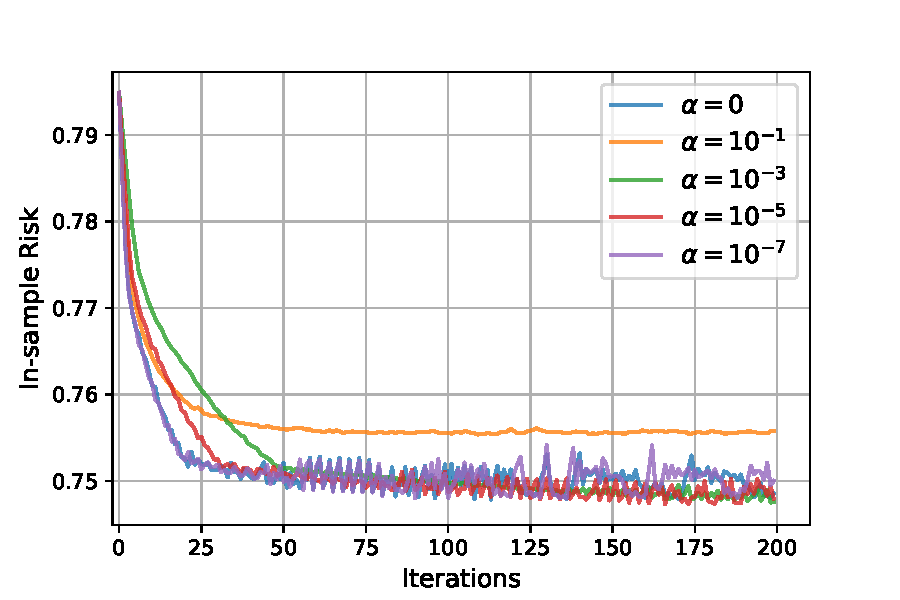
\includegraphics[width=0.46\textwidth]{Images/convergence_toy.pdf}
%     \caption{Caption}
%     \label{fig:toy_example_cvgence}
% \end{figure}
\begin{figure*}[!ht]
\begin{center}

\textbf{Adversarial Training, CIFAR-10 dataset results}
 \begin{small}
\begin{tabular}{c|c|ccc} 
\textbf{ Models} & \textbf{Acc. }&\textbf{$\textrm{APGD}_\textrm{CE}$}& \textbf{$\textrm{APGD}_\textrm{DLR}$} & \textbf{Rob. Acc.} \\ \hline
 1 & $81.9\%$ &	$47.6\%$ & $47.7\%$ & $45.6\%$ \\ 
 2 & $81.9\%$ & $49.0\%$ & ${49.6\%}$ & ${47.0\%}$\\ 
  3 & ${81.7\%}$& ${49.0\%}$ & $49.3\%$ & ${46.9\%}$\\
    4 & $\bm{82.6\%}$& $\bm{49.7\%}$ & $\bm{49.8}\%$ & $\bm{47.2\%}$\\

\end{tabular}
\end{small}\\
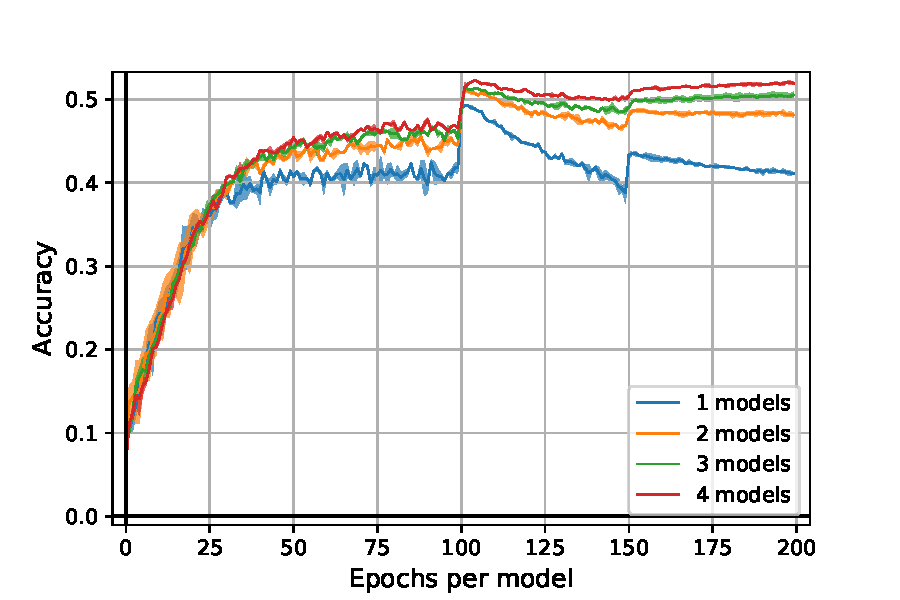
\includegraphics[width=0.35\textwidth]{Images/robust_acc_finalrun_ResNet18_1024_200_0.001.pdf}\includegraphics[width=0.35\textwidth]{Images/standard_acc_finalrun_ResNet18_1024_200_0.001.pdf} 
  

\textbf{TRADES, CIFAR-10 dataset results}

 \begin{small}
\begin{tabular}{c|c|ccc} 
\textbf{ Models} & \textbf{Acc. }&\textbf{$\textrm{APGD}_\textrm{CE}$}& \textbf{$\textrm{APGD}_\textrm{DLR}$} & \textbf{Rob. Acc.} \\ \hline
 1 &  $79.6\%$ &$50.9\%$& $48.9\%$ &$48.3\%$ \\ 
 2 & $80.3\%$& $52.3\%$ &$51.2\%$ &$50.2\%$\\ 
  3 & $80.7\%$& $52.8\%$ &$51.7\%$ &$50.7\%$\\
    4 & \bm{$80.9\%$} & \bm{$53.0\%$}& \bm{$51.8\%$}& \bm{$50.8\%$}\\

\end{tabular}
\end{small}

\includegraphics[width=0.35\textwidth]{Images/robust_acc_CIFAR10_final_cam_ready_bisss_ResNet18_1024_200_0.001.pdf}\includegraphics[width=0.35\textwidth]{Images/standard_acc_CIFAR10_final_cam_ready_bisss_ResNet18_1024_200_0.001.pdf} 
  

\textbf{Adversarial Training, CIFAR-100 dataset results}
 \begin{small}
\begin{tabular}{c|c|ccc} 
\textbf{ Models} & \textbf{Acc. }&\textbf{$\textrm{APGD}_\textrm{CE}$}& \textbf{$\textrm{APGD}_\textrm{DLR}$} & \textbf{Rob. Acc.} \\ \hline
 1 & $55.2\%$& $24.1\%$& $23.8\%$ & $22.5\%$\\ 
 2 & $55.2\%$ & $25.3\%$ &$26.1\%$ &$23.6\%$\\ 
  3 & \bm{$55.4\%$} & $25.7\%$ &$26.8\%$ &$24.2\%$\\
    4 & $55.3\%$ & \bm{$26.0\%$} & \bm{$27.5\%$}& \bm{$24.5\%$}\\

\end{tabular}
\end{small}
\includegraphics[width=0.35\textwidth]{Images/robust_acc_CIFAR100_finalrun_ResNet18_1024_200_0.001.pdf}\includegraphics[width=0.35\textwidth]{Images/standard_acc_CIFAR100_finalrun_ResNet18_1024_200_0.001.pdf} 


 \caption{Upper plots: Adversarial Training, CIFAR-10 dataset results. Middle plots:  TRADES, CIFAR-10 dataset results. Bottom plots: CIFAR-100 dataset results. {On left}: Comparison of our algorithm with a standard adversarial training (one model). We reported the results for the model with the best robust accuracy obtained over two independent runs because adversarial training might be unstable. Standard and Robust accuracy (respectively in the middle and on right) on CIFAR-10 test images in function of the number of epochs per classifier with $1$ to $3$ ResNet18 models. The performed attack is PGD with $20$ iterations and $\varepsilon=8/255$.}
\label{fig:results_cifar}

\end{center}
\end{figure*}

To evaluate the convergence of our algorithms, we compute the adversarial risk of our mixture for each iteration of both the oracle and regularized algorithms. Figure~\ref{fig:toy_example} illustrates the convergence of the algorithms w.r.t the regularization parameter. We observe that the risk for both algorithms converge. Moreover, they converge towards the oracle minimizer when the regularization parameter $\alpha$ goes to $0$.

Finally, to demonstrate the improvement randomized techniques offer against deterministic defenses, we plot in Figure~\ref{fig:toy_example} (right) the minimum adversarial risk for both randomized and deterministic classifiers w.r.t. $\varepsilon$. The adversarial risk is strictly better for randomized classifier whenever the adversarial budget $\varepsilon$ is bigger than $2$. This illustration validates our analysis of Theorem~\ref{thm:duality-rand}, and motivates a in depth study of a more challenging framework, namely image classification with neural networks.

% \begin{figure}[ht]
%     \centering
%     \includegraphics[width=0.46\textwidth]{Images/risk_toy.pdf}
%     \caption{Caption}
%     \label{fig:toy_example_risk}
% \end{figure}

\subsection{CIFAR Datasets}

% \begin{figure*}[!ht]
% \begin{center}

% \vskip 0.15in
%  \begin{minipage}[ht!]{0.39\textwidth}
%  \begin{scriptsize}
% \begin{tabular}{c|c|ccc} 
% \textbf{ Models} & \textbf{Acc. }&\textbf{$\textrm{APGD}_\textrm{CE}$}& \textbf{$\textrm{APGD}_\textrm{DLR}$} & \textbf{Rob. Acc.} \\ \hline
%  1 & $81.9\%$ &	$47.6\%$ & $47.7\%$ & $45.6\%$ \\ 
%  2 & $81.9\%$ & $49.0\%$ & ${49.6\%}$ & ${47.0\%}$\\ 
%   3 & ${81.7\%}$& ${49.0\%}$ & $49.3\%$ & ${46.9\%}$\\
%     4 & $\bm{82.6\%}$& $\bm{49.7\%}$ & $\bm{49.8}\%$ & $\bm{47.2\%}$\\

% \end{tabular}
% \end{scriptsize}
%   \end{minipage}\begin{minipage}[!ht]{0.61\textwidth}
% \includegraphics[width=0.49\textwidth]{Images/robust_acc_finalrun_ResNet18_1024_200_0.001.pdf}\includegraphics[width=0.49\textwidth]{Images/standard_acc_finalrun_ResNet18_1024_200_0.001.pdf} 
%   \end{minipage}
  
% Adversarial Training, CIFAR-10 dataset results

% \vskip 0.15in
%  \begin{minipage}[ht!]{0.39\textwidth}
%  \begin{scriptsize}
% \begin{tabular}{c|c|ccc} 
% \textbf{ Models} & \textbf{Acc. }&\textbf{$\textrm{APGD}_\textrm{CE}$}& \textbf{$\textrm{APGD}_\textrm{DLR}$} & \textbf{Rob. Acc.} \\ \hline
%  1 &  $79.6\%$ &$50.9\%$& $48.9\%$ &$48.3\%$ \\ 
%  2 & $80.3\%$& $52.3\%$ &$51.2\%$ &$50.2\%$\\ 
%   3 & $80.7\%$& $52.8\%$ &$51.7\%$ &$50.7\%$\\
%     4 & \bm{$80.9\%$} & \bm{$53.0\%$}& \bm{$51.8\%$}& \bm{$50.8\%$}\\

% \end{tabular}
% \end{scriptsize}
%   \end{minipage}\begin{minipage}[!ht]{0.61\textwidth}
% \includegraphics[width=0.49\textwidth]{Images/robust_acc_CIFAR10_final_cam_ready_bisss_ResNet18_1024_200_0.001.pdf}\includegraphics[width=0.49\textwidth]{Images/standard_acc_CIFAR10_final_cam_ready_bisss_ResNet18_1024_200_0.001.pdf} 
%   \end{minipage}
  
% TRADES, CIFAR-10 dataset results
% \vskip 0.15in
%  \begin{minipage}[ht!]{0.39\textwidth}
%  \begin{scriptsize}
% \begin{tabular}{c|c|ccc} 
% \textbf{ Models} & \textbf{Acc. }&\textbf{$\textrm{APGD}_\textrm{CE}$}& \textbf{$\textrm{APGD}_\textrm{DLR}$} & \textbf{Rob. Acc.} \\ \hline
%  1 & $55.2\%$& $24.1\%$& $23.8\%$ & $22.5\%$\\ 
%  2 & $55.2\%$ & $25.3\%$ &$26.1\%$ &$23.6\%$\\ 
%   3 & \bm{$55.4\%$} & $25.7\%$ &$26.8\%$ &$24.2\%$\\
%     4 & $55.3\%$ & \bm{$26.0\%$} & \bm{$27.5\%$}& \bm{$24.5\%$}\\

% \end{tabular}
% \end{scriptsize}
%   \end{minipage}\begin{minipage}[!ht]{0.61\textwidth}
% \includegraphics[width=0.49\textwidth]{Images/robust_acc_CIFAR100_finalrun_ResNet18_1024_200_0.001.pdf}\includegraphics[width=0.49\textwidth]{Images/standard_acc_CIFAR100_finalrun_ResNet18_1024_200_0.001.pdf} 
%   \end{minipage}
%   Adversarial Training, CIFAR-100 dataset results

%  \caption{Upper plots: Adversarial Training, CIFAR-10 dataset results. Middle plots:  TRADES, CIFAR-10 dataset results. Bottom plots: CIFAR-100 dataset results. {On left}: Comparison of our algorithm with a standard adversarial training (one model). We reported the results for the model with the best robust accuracy obtained over two independent runs because adversarial training might be unstable. Standard and Robust accuracy (respectively in the middle and on right) on CIFAR-10 test images in function of the number of epochs per classifier with $1$ to $3$ ResNet18 models. The performed attack is PGD with $20$ iterations and $\varepsilon=8/255$.}
% \label{fig:results_cifar}

% \end{center}
% \end{figure*}

% Adversarial examples are known to be easily transferrable from one model to another~\cite{tramer2017space}. To counter this and support our theoretical claims, we propose an heuristic algorithm (see Algorithm~\ref{algo:heuristic}) to train a robust mixture of $L$ classifiers. We alternatively train these classifiers with adversarial examples against the current mixture and update the probabilities of the mixture according to the algorithms we proposed in Section~\ref{sec:proposed-algo}. More details on the heuristic algorithm are available in Appendix~\ref{sec:additional-xp}. 
% \begin{algorithm}[h!]
% \small
% \SetAlgoLined
% $L$: number of models, $T$: number of iterations,\\
% $T_\theta$: number of updates for the models $\bm{\theta}$,\\
% $T_\lambda$: number of updates for the mixture $\bm{\lambda}$,\\ $\bm{\lambda}_0=(\lambda_0^1,\dots\lambda_0^L),~\bm{\theta}_0=(\theta_0^1,\dots\theta_0^L)$\\
%  \For{$t=1,\dots,T$}{
%  Let $B_t$ be a batch of data.\\
% \eIf{$t \mod (T_\theta L+1)\neq 0$}{
% $k$ sampled uniformly in $\{1,\dots,L\}$\\
% $\Tilde{B}_t\leftarrow$ Attack of images in $B_t$ for the  model $(\bm{\lambda}_t,\bm{\theta}_t)$\\
% $\theta^t_k\leftarrow$ Update $\theta^{t-1}_k$ with $\Tilde{B}_t$ for fixed $\bm{\lambda}_t$ with a SGD step}{
% $\bm{\lambda}_t\leftarrow$Update $\bm{\lambda}_{t-1}$ on $B_t$ for fixed $\bm{\theta}_t$
% with oracle or regularized algorithm with $T_\lambda$ iterations.
% }
%   }
%  \caption{Adversarial Training for Mixtures}
 
%  \label{algo:heuristic}
% \end{algorithm}

\paragraph{Experimental Setup.} We now implement our heuristic algorithm (Alg.~\ref{algo:heuristic}) on CIFAR-10 and CIFAR-100 datasets for both Adversarial Traning~\citep{madry2017towards} and TRADES~\citep{zhang2019theoretically} loss. To evaluate the performance of Algorithm~\ref{algo:heuristic}, we trained from $1$ to $4$ ResNet18~\citep{He_2016_CVPR} models on $200$ epochs per model\footnote{$L\times200$ epochs in total, where $L$ is the number of models.}. We study the robustness with regards to $\ell_\infty$ norm and fixed adversarial budget $\varepsilon=8/255$. The attack we used in the inner maximization of the training is an adapted (adaptative) version of PGD for mixtures of classifiers with $10$ steps. Note that for one single model, Algorithm~\ref{algo:heuristic} exactly corresponds to adversarial training~\citep{madry2017towards} or TRADES. For each of our setups, we made two independent runs and select the  best one. The training time of our algorithm is around four times longer than a standard Adversarial Training (with PGD 10 iter.) with two models, eight times with three models and twelve times with four models. We trained our models with a batch of size  $1024$ on $8$ Nvidia V100 GPUs. 

\paragraph{Optimizer.} For each of our models, The optimizer we used in all our implementations is SGD with learning rate set to $0.4$ at epoch $0$ and is divided by $10$ at half training then by $10$ at the three quarters of training. The momentum is set to $0.9$ and the weight decay to $5\times10^{-4}$. The batch size is set to $1024$. 
\paragraph{Adaptation of Attacks.} Since our classifier is randomized, we need to adapt the attack accordingly. To do so we used the expected loss:
\begin{align*}
\Tilde{\loss}\left((\bm{\lambda},\bm{\theta}),(x,y)\right) = \sum_{k=1}^L \lambda_k \loss(\theta_k,(x,y))
\end{align*}
to compute the gradient in the attacks, regardless the loss (DLR or cross-entropy). For the inner maximization at training time, we used a PGD attack on the cross-entropy loss with $\varepsilon=0.03$. For the final evaluation, we used the untargeted $DLR$ attack with default parameters.
\paragraph{Regularization in Practice.} The entropic regularization in higher dimensional setting need to be adapted to be more likely to find adversaries. To do so, we computed PGD attacks with only $3$ iterations with $5$ different restarts instead of sampling uniformly $5$ points  in the $\ell_\infty$-ball. In our experiments in the main paper, we use a regularization parameter $\alpha=0.001$. The learning rate for the minimization on $\bm{\lambda}$ is always fixed to $0.001$. 
\paragraph{Alternate Minimization Parameters.} Algorithm~\ref{algo:heuristic} implies an alternate minimization algorithm. We set the number of updates of $\bm{\theta}$ to $T_\theta = 50$ and, the update of $\bm{\lambda}$ to $T_\lambda = 25$. 

\subsection{Effect of the Regularization}
In this subsection, we experimentally investigate the effect of the regularization. In Figure~\ref{fig:xp-regularization}, we notice, that the regularization has the effect of stabilizing, reducing the variance and improving the level of the robust accuracy for adversarial training for mixtures (Algorithm~\ref{algo:heuristic}). The standard accuracy curves are very similar in both cases.



\paragraph{Evaluation Protocol.} At each epoch, we evaluate the current mixture on test data against PGD attack  with $20$ iterations. To select our model and avoid overfitting~\citep{rice2020overfitting}, we kept the most robust against this PGD attack.
To make a final evaluation of our mixture of models, we used an adapted version of $\textrm{AutoPGD}$ untargeted attacks~\citep{croce2020reliable} for randomized classifiers with both Cross-Entropy (CE) and Difference of Logits Ratio (DLR) loss. For both attacks, we made $100$ iterations and $5$ restarts.

\paragraph{Results.} The results are presented in Figure~\ref{fig:results_cifar}. We remark our algorithm outperforms a standard adversarial training in all the cases by more $1\%$ on CIFAR-10 and CIFAR-100, without additional loss of standard accuracy as it is attested by the left figures. On TRADES, the gain is even more important by more than $2\%$ in robust accuracy. Moreover, it seems our algorithm, by adding more and more models, reduces the overfitting of adversarial training. It also appears that robustness increases as the number of models increases. So far, experiments are computationally very costful and it is difficult to raise precise conclusions. Further, hyperparameter tuning ~\citep{gowal2020uncovering} such as architecture, unlabeled data~\citep{carmon2019unlabeled} or activation function may still increase the results.





% \begin{figure*}[!ht]
% \begin{center}


% \label{table:results}
% \vskip 0.15in
%  \begin{minipage}[!ht]{0.39\textwidth}
%  \begin{scriptsize}
% \begin{tabular}{c|c|ccc} 
% \textbf{ Models} & \textbf{Acc. }&\textbf{$\textrm{APGD}_\textrm{CE}$}& \textbf{$\textrm{APGD}_\textrm{DLR}$} & \textbf{Rob. Acc.} \\ \hline
%  1 & $81.9\%$ &	$47.6\%$ & $47.7\%$ & $45.6\%$ \\ 
%  2 & $81.9\%$ & $49.0\%$ & ${49.6\%}$ & ${47.0\%}$\\ 
%   3 & ${81.7\%}$& ${49.0\%}$ & $49.3\%$ & ${46.9\%}$\\
%     4 & $\bm{82.6\%}$& $\bm{49.7\%}$ & $\bm{49.8}\%$ & $\bm{47.2\%}$\\

% \end{tabular}
% \end{scriptsize}
%   \end{minipage}\begin{minipage}[!ht]{0.61\textwidth}
% \includegraphics[width=0.49\textwidth]{Images/robust_acc_finalrun_ResNet18_1024_200_0.001.pdf}\includegraphics[width=0.49\textwidth]{Images/standard_acc_finalrun_ResNet18_1024_200_0.001.pdf} 
%   \end{minipage}
  
% \caption{On left: Comparison of our algorithm with a standard adversarial training (one model). We reported the results for the model with the best robust accuracy obtained over two independent runs because adversarial training might be unstable. Standard and Robust accuracy ( respectively in the center and on left) on CIFAR-10 test images in function of the number of epochs per classifier with $1$ to $3$ ResNet18 models. The performed attack is PGD with $20$ iterations and $\varepsilon=8/255$.}
% \label{fig:results_cifar}
% \end{center}
% \end{figure*}











% \begin{figure}[!ht]
% \includegraphics[width=0.46\textwidth]{Images/standard_acc_finalrun_ResNet18_1024_200_0.001.pdf}    \caption{Standard accuracy on CIFAR-10 test images in function of the number of epochs per classifier with $1$ to $3$ ResNet18 models.}
%     \label{fig:plot_standard_acc}
% \end{figure}

% \begin{figure}[!ht]
% \includegraphics[width=0.46\textwidth]{Images/robust_acc_finalrun_ResNet18_1024_200_0.001.pdf}    \caption{Robust accuracy on CIFAR-10 test images in function of the number of epochs per classifier with $1$ to $3$ ResNet18 models. The attack performed is PGD with $20$ iterations and $\varepsilon=8/255$.}
%     \label{fig:plot_robust_acc}
% \end{figure}



% mettre ca au propre mais les resultats sont la!!

% setup: ResNet18 ou WRN28x10

% Details in supmat: loss +lr + format of training etc

% In supmat: 
% \begin{enumerate}
%     \item details HP (attack + training)
%     \item details runtime
%     \item additional results (with other attacks maybe + other archis...)
    
    
% \end{enumerate}
% Epochs 100

\section{Conclusion}
We presented several settings for online attacks on contextual bandits.
We showed that an attacker can force any contextual bandit algorithm to almost always pull an arbitrary target arm $a^{\dagger}$ with only sublinear modifications of the rewards. When the attacker can only modify the contexts, we prove that \linucb can still be attacked and made to almost always pull an arm in $A^{\dagger}$ by adding sublinear perturbations to the contexts. 
When the attacker can only attack a single context, we derive a feasibility condition for the attacks and we introduce a method to compute some attacks of small instantaneous cost for \linucb, \epsgreedy and \lints.
To the best of our knowledge, this paper is the first to describe effective attacks on the contexts of contextual bandit algorithms. Our numerical experiments, conducted on both synthetic and real-world data, validate our results and show that the attacks on all contexts are actually effective on several algorithms and with more permissible settings. 





\begin{subappendices}
% !TEX root = main.tex

\section{Appendix: Proofs}
In this appendix, we present the proofs of different theoretical results presented in the paper.
\subsection{Proof of Proposition \ref{prop:reward_attack}}\label{app:proof_prop_rewd_attack}

\begin{prop*}
	For any $\delta\in(0, 1/K]$, when using Contextual ACE algorithm (Alg. ~\ref{alg:attacker_rewards}) with perturbed rewards $\tilde{r}^{1}$, with probability at least $1-K\delta$, algorithm $\mathfrak{A}$ pulls \changelm{an arm in $A^{\dagger}$} for $T - o(T)$ time steps and the total cost of attacks is $o(T)$.
\end{prop*}

\begin{proof}
	Let us consider the contextual bandit problem $\mathcal{A}_{1}$, with $K$ arms with contexts $x\in \mathcal{D}$ such that every arm in \changelm{$a^\dagger\in A^\dagger$ has mean reward $\langle \theta_{a^{\dagger}}, x\rangle$} and all other arms has mean $0$. Then the regret of algorithm $\mathfrak{A}$ for this bandit problem is upper-bounded with probability at least $1 - \delta$ by a function $f_{\mathfrak{A}}(T)$ such that $f_{\mathfrak{A}}(T) = o(T)$. In addition, the reward process fed to Alg. $\mathfrak{A}$ by the attacker is a stationary reward process with $\sigma^{2}$-subgaussian noise. Therefore, the number of times algorithm $\mathfrak{A}$ pulls an arm \changelm{not in $A^{\dagger}$ is upper-bounded by \changee{$f_{\mathfrak{A}}(T)/\min_{x\in \mathcal{D}} \Delta(x)$ where for every context $x\in\mathcal{D}$, let $a
^{\dagger}_{\star}(x) := \arg\max_{a\in A^{\dagger}} \langle x, \theta_{a}\rangle$ and $\Delta(x) = \langle x, \theta_{a^{\dagger}_{\star}(x)}\rangle - \max_{a\in A^{\dagger}, a\neq a_{\star}^{\dagger}(x)} \langle x, \theta_{a}\rangle$}}. 

\changelm{In addition, the total cost of the attack is upper-bounded by $\max_{a\in \llbracket 1, K\rrbracket} \max_{x\in \mathcal{D}} |\langle x, \theta_{a}\rangle| (T - N_{A^{\dagger}}(T))$ where $N_{A^{\dagger}}(T)$ is the number of times an arm  in $A^{\dagger}$ has been pulled up to time $T$. Thanks to the previous argument, $T - N_{A^{\dagger}}(T) \leq  f_{\mathfrak{A}}(T)/\min_{x\in \mathcal{D}}\Delta(x)$.}
\end{proof}
% \subsection{Proof of Proposition \ref{prop:cost_attack_all_ctx}:}
% \begin{proof}
% The bound of the number of times the arm $a^*$ is the same as for proposition \ref{prop:reward_attack}.
% As the attacker only attacks when the arm $a^{\star}$ is not pulled and the contexts are bounded by 1, the total cost of each attack is upper bounded by $\delta$, hence the bound on the total cost of the attacks.

% \end{proof}

\subsection{Proof of Proposition \ref{prop:cost_attack_all_ctx}}\label{app:proof_attack_all_ctx}

\begin{prop*}
Using the attack described in Alg.~\ref{alg:context_attack_protocol}, for any $\delta\in (0, 1/K]$, with probability at least $1 - K\delta$, the number of times \linucb does not pull \changelm{an arm in $A^{\dagger}$} is at most:
\begin{align*}
    \sum_{j\changelm{\notin A^{\dagger}}} N_{j}(T) \leq 32K^{2}\left( \frac{\lambda}{\alpha^{2}} + \sigma^{2}d\log\left(\frac{\lambda d + TL^2\alpha^{2}}{d\lambda\delta}\right) \right)^{3}
\end{align*}
with $N_{j}(T)$ the number of times arm $j$ has been pulled after $T$ steps, $|| \theta_{a}|| \leq S$ for all arms $a$, $\lambda$ the regularization parameter of \linucb and for all $x\in \mathcal{D}$, $||x||_{2}\leq L$. The total cost for the attacker is bounded by:
\begin{align*}
    \sum_{t=1}^{T} c_{t} \leq \frac{64K^{2}}{\nu}\left( \frac{\lambda}{\alpha^{2}} + \sigma^{2}d\log\left(\frac{\lambda d + TL^2\alpha^{2}}{d\lambda\delta}\right) \right)^{3}
\end{align*}
\end{prop*}

\begin{proof}
Let $a_{t}$ be the arm pulled by \linucb at time $t$. For each arms $a$, let $\tilde{\theta}_a(t)$ be the result of the linear regression with the attacked context and $\hat{\theta}_{a}(t, \lambda/\alpha^{2})$ the one with the unattacked context and a regularization of $\frac{\lambda}{\alpha^{2}}$. At any time step $t$, we can write, for all $a\changebrtwo{\not\in A^\dagger}$:

\begin{align*}
\tilde{\theta}_a(t) &=  \left(\lambda I_d + \sum_{l=0, a_{l} = a}^{t} \alpha^{2} x_l x_l^{\intercal}\right)^{-1} \sum_{k=0, a_{k} = a}^{t} r_k \alpha x_{k} \\
&= \frac{1}{\alpha} \left(\frac{\lambda}{\alpha^2} I_d + \sum_{k=0, a_{k} = a}^t x_k x_k^{\intercal}\right)^{-1} \sum_{k=0, a_{k} = a}^t r_k x_k \\
&= \frac{\hat{\theta}_{a}(t,\lambda/\alpha^{2})}{\alpha}
\end{align*}
\changelm{We also note that, since the contexts are not modified for arms in  $a^\dagger\in A^\dagger$: $\tilde{\theta}_{a^\dagger}(t)=\hat{\theta}_{a^\dagger}(t,\lambda)$. In addition, for any context $x$ and arm $a\notin A^\dagger$, the exploration term used by \linucb becomes:}
\begin{align}
    ||x||_{\tilde{V}_{a,t}^{-1}}&= \frac{1}{\alpha} ||x||_{\hat{V}_{a,t}^{-1}}
\end{align}
where $\tilde{V}_{a,t} = \lambda I_d + \sum_{l=0, a_{l} = a}^{t} \alpha^{2} x_l x_l^{\intercal}$ and $\hat{V}_{a,t}^{-1} =\lambda/ \alpha^2 I_d + \sum_{k=0, a_{k} = a}^t x_k x_k^{\intercal}$. For a time $t$, if presented with context $x_{t}$ \linucb pulls arm \changelm{$a_{t} \notin A^{\dagger}$,} we have:
\begin{align*}
\alpha\left(\left\langle \hat{\theta}_{a^\dagger}(t), x_{t} \right\rangle +\beta_{a^\dagger}(t)||x_t||_{V_{a^\dagger,t}^{-1}}\right)\leq \left\langle \hat{\theta}_{a_{t}}(t, \lambda/\alpha^{2}), x_{t} \right\rangle +  \beta_{a_{t}}(t)||x_{t}||_{\hat{V}_{a_{t},t}^{-1}} 
\end{align*}

As \changelm{$\alpha = \frac2\nu\geq\min_{a^\dagger\in A^\dagger}\frac{2}{\left\langle \theta_{a^\dagger}, x_{t} \right\rangle}$}, we deduce that on the event that the confidence sets (Theorem $2$ in \cite{abbasi2011improved}) hold for arm $a^{\star}$: 
\begin{align*}
    2&\leq\left\langle \hat{\theta}_{a_{t}}(t, \lambda/\alpha^{2}), x_{t} \right\rangle +  \beta_{a_{t}}(t)||x_{t}||_{\hat{V}_{a_{t},t}^{-1}}\leq \langle\theta_{a_{t}}, x_{t}\rangle+2\beta_{a_{t}}(t)||x_{t}||_{\hat{V}_{a_{t},t}^{-1}}
\end{align*}
Thus, $1 \leq 2 - \langle\theta_{a_{t}}, x_{t}\rangle \leq 2\beta_{a_{t}}(t)||x_{t}||_{\hat{V}_{a_{t},t}^{-1}}$. Therefore,
\begin{align*}
    \sum_{t=1}^{T} \mathds{1}_{\{a_{t}\notin A^{\dagger}\}} &\leq \sum_{t=1}^{T} \min(2\beta_{a_{t}}(t)||x_{t}||_{\hat{V}_{a_{t},t}^{-1}},1)\mathds{1}_{\{a_{t} \notin A^{\dagger}\}}\\
    &\leq \sum_{j\notin A^{\dagger}} 2\beta_{j}(T)\sqrt{\sum_{t=1}^{T}\mathds{1}_{\{a_{t}=j\}}\sum_{t=1, a_{t}=j}^{T} \min(1, ||x_{t}||^{2}_{\hat{V}_{j,t}^{-1}})}&
  \end{align*}
  But using Lemma $11$ from \cite{abbasi2011improved} and the bound on the $\beta_{j}(T)$ for all arms $j$, we have with Jensen inequality:
  \begin{align*}
    \sum_{t=1}^{T} \mathds{1}_{\{a_{t}\notin A^{\dagger}\}} \leq &4\sqrt{K\sum_{t=1}^{T} \mathds{1}_{\{a_{t}\notin A^{\dagger}\}}d\log\left(1 + \frac{\alpha^2TL^2}{\lambda d}\right)}\\
    &\times\Big( \sqrt{\lambda/\alpha^{2}} S + \sigma\sqrt{2\log(1/\delta) + d\log(1 + \frac{\alpha^2TL^2}{\lambda d})}\Big)
\end{align*}
\end{proof}



\subsection{Proof of Theorem \ref{thm:feasibility_attack_one_user}}\label{app:feasibility_attack_one_user}

\begin{thm*}
For any $\xi>0$, Problem \eqref{eq:attack_one_user} is feasible if and only if:
\begin{align}\label{eq:feasibilty_condition_bis}
\exists \theta \in  \changelm{\bigcup_{a^\dagger\in A^{\dagger}}}\mathcal{C}_{t, a^{\dagger}}, \qquad \theta\not\in \text{Conv}\left( \bigcup_{a\notin A^{\dagger}} \mathcal{C}_{t,a}\right)
\end{align}
	where for every arm $a$,  $\mathcal{C}_{t,a} := \big\{\theta \mid ||\theta - \hat{\theta}_{a}(t)||_{\tilde{V}_{a,t}} \leq \beta_{a}(t) \big\}$ with $\hat{\theta}_{a}(t)$ the least squares estimate for arm $a$ built by \linucb and 
	$$\tilde{V}_{a,t} = \lambda I_{d} + \sum_{l=1, x_{l}\neq x^{\dagger}}^{t} \mathds{1}_{\{a_{l} = a\}}x_{l}x_{l}^{\intercal} + \sum_{l=1, x_{l}= x^{\dagger}}^{t} \mathds{1}_{\{a_{l} = a\}}\tilde{x}_{l}\tilde{x}_{l}^{\intercal} $$ 
	the design matrix of \linucb at time $t$ for all arms $a$ (where $\tilde{x}_{l}$ is the modified context)
\end{thm*}

\begin{proof}
The proof of Theorem \ref{thm:feasibility_attack_one_user} is decomposed in two parts. 

First, let us assume that Equation \eqref{eq:feasibilty_condition_bis} is satisfied. Then, \changebrtwo{let us define $a^\dagger \in A^\dagger$ such that} $\theta \in \mathcal{C}_{t,a^{\dagger}}\setminus \text{Conv}\left( \bigcup_{a\notin A^{\dagger}} \mathcal{C}_{t,a}\right) $, then by the theorem of separation of convex sets applied to $\mathcal{C}_{t,a^{\dagger}}$ and $\{ \theta \}$. There exists a vector $v$ and $c_{1}< c_{2}$ such that for all $y \in \text{Conv}\left( \bigcup_{a\neq a^{\dagger}} \mathcal{C}_{t,a}\right)$:
\begin{align*}
\left\langle y, v\right\rangle \leq c_{1} < c_{2} \leq \left\langle \theta,v\right\rangle.
\end{align*}
Hence, for $\xi>0$ we have that for $\tilde{v} = \frac{\xi}{c_{2}-c_{1}} v$ that:
\begin{align*}
    \left\langle y, \tilde{v}\right\rangle + \xi \leq \left\langle \theta, \tilde{v} \right\rangle
\end{align*}
So the problem is feasible.

Secondly, let us assume that an attack is feasible. Then there exists a vector $y$ such that:
\begin{align}
    \changebrtwo{\max_{a^\dagger \in A^\dagger}}\max_{\theta\in \mathcal{C}_{t,a^{\dagger}}} \left\langle y, \theta\right\rangle > c_{1} := \max_{a\notin A^{\dagger}} \max_{\theta\in \mathcal{C}_{t,a}} \left\langle y, \theta\right\rangle
    \label{eq:feasible_in_proof}
\end{align}
% \changebrtwo{We can define $a^\dagger = \argmax_{a\neq a^{\dagger}} \max_{\theta\in \mathcal{C}_{t,a}}$, which verifies:}
%     \begin{align*}
%     \max_{\theta\in \mathcal{C}_{t,a^{\dagger}}} \left\langle y, \theta\right\rangle > c_{1} := \max_{a\neq a^{\dagger}} \max_{\theta\in \mathcal{C}_{t,a}} \left\langle y, \theta\right\rangle
%     \end{align*}
\changelm{
	Let us reason by contradiction. We assume that $ \bigcup_{a\in A^{\dagger}}\mathcal{C}_{t,a^{\dagger}} \subset \text{Conv}\left( \bigcup_{a\notin A^{\dagger}} \mathcal{C}_{t,a}\right)$ and consider 
	\begin{align*}
	    \theta^*\in\bigcup_{a\in A^{\dagger}}\mathcal{C}_{t,a^{\dagger}}\text{ such that } \left\langle y, \theta^*\right\rangle=\max_{a^\dagger \in A^\dagger}\max_{\theta\in \mathcal{C}_{t,a^{\dagger}}} \left\langle y, \theta\right\rangle
	\end{align*}
	As we assumed $ \bigcup_{a\in A^{\dagger}}\mathcal{C}_{t,a^{\dagger}} \subset \text{Conv}\left( \bigcup_{a\notin A^{\dagger}} \mathcal{C}_{t,a}\right)$, there exists $n\in\mathbb{N}^{\star}$, $\lambda_{1},\cdots, \lambda_{n}\geq 0$ and $\theta_{1}, \cdots, \theta_{n}\in \bigcup_{a\notin A^{\dagger}} \mathcal{C}_{t,a}$ \text{such that}
	\begin{align*}
	    \theta^* = \sum_{i=1}^{n} \lambda_{i}\theta_{i}\text{ and } \sum_{i=1}^{n} \lambda_{i} = 1
	\end{align*}
	Thus
\begin{align}
    \left\langle y, \theta^*\right\rangle = \sum_{i} \lambda_{i} \left\langle y, \theta_{i} \right\rangle \leq c_{1}\sum_{i=1}^{n} \lambda_{i} = c_{1}\label{cdas}
\end{align}
\changebrtwo{We assumed that the problem is feasible, so $c_{1}<  
\left\langle y, \theta^*\right\rangle$ according to Eq.~\ref{eq:feasible_in_proof}. It} contradicts Eq. \ref{cdas}.
}
\end{proof}


\subsection{Condition of Sec.~\ref{sec:attack_one_context}}\label{app:condition_linear}
\begin{figure}[ht]
\centering
    \includegraphics[width=0.5\linewidth]{sections/appendix/nips2020-bandits/images/condition_feasibility_acceptance.pdf}
	\caption{Illustrative example of condition \eqref{eq:feasibilty_condition}. The target arm is arm $3$ or $5$ and the dashed black line is the convex hull of the other confidence sets. The ellipsoids are the confidence sets $\mathcal{C}_{t,a}$ for each arm $a$. If we consider only arms $\{1,2,4,5\}$, and we use $5$ as the target arm, the condition \eqref{eq:feasibilty_condition} is satisfied as there is a $\theta$ outside the convex hull of the other confidence sets. On the other hand, if we consider arms $\{1,2,3,4\}$ and we use $3$ as the target arm, the condition is not satisfied anymore. \label{fig:feasibility_condition}}
\end{figure}

\changebr{Let us assume that \changebrtwo{there is an arm in $a^\dagger\in A^\dagger$ which is} optimal for some contexts. More formally, there exists a subspace $V\subset \mathcal{D}$ such that:} 
\begin{equation*}    
\forall x\in V, \exists a^{\dagger}_{\star}(x)\in A^\dagger, \forall a\in \llbracket 1, K\rrbracket\setminus\{a^{\dagger}_{\star}(x)\} \qquad \langle x, \theta_{a^{\dagger}_{\star}(x)}\rangle > \left\langle x, \theta_{a}\right\rangle.
\end{equation*}
\changebr{We also assume that} the distribution of the contexts is such that, for all $t$, $\mu := \mathbb{P}\left(x_{t}\in V\right) >0$.
Then\changebr{,} the regret is lower-bounded in expectation by:
\begin{align*}
    \mathbb{E}(R_{T}) &= \mathbb{E}\left(\sum_{t=1}^{T} \mathds{1}_{\{x_{t}\in V\}}\big( \left\langle x_{t}, \theta_{a^{\dagger}_{\star}(x_{t})} - \theta_{a_{t}}\right\rangle\big)\right) \geq \mu m(T) \min_{x\in V} \max_{a\neq a^{\dagger}_\star(x)} \langle \theta_{a^{\dagger}_{\star}(x)} - \theta_{a}, x\rangle
\end{align*}
where $m(T)$ is the expected number of times $t\leq T$ such that condition \eqref{eq:feasibilty_condition} is not met. \changebr{\linucb guarantees that}  $\mathbb{E}(R_{T}) \leq \mathcal{O}(\sqrt{T})$ for every $T$. Hence, 
\begin{align*}
    m(T) \leq \mathcal{O}\left(\frac{\sqrt{T}}{\mu\min_{x\in V}\max_{a\neq a^{\dagger}_\star(x)} \langle \theta_{a^{\dagger}_{\star}(x)} - \theta_{a}, x\rangle}\right)
\end{align*}
This means that, in an unattacked problem, condition \eqref{eq:feasibilty_condition} is met $T - \mathcal{O}(\sqrt{T})$ times. On the other hand, when the algorithm is attacked the regret of \linucb is not sub-linear as the confidence bound for the target arm is not valid anymore. Hence we cannot provide the same type of guarantees for the attacked problem.



% !TEX root = main.tex
\section{Experiments}

\subsection{Datasets and preprocessing}\label{app:experiments_setup}
% \todoe{This section also explain how we preprocessed the real-wolrd datasets too.}

We present here the datasets used in the article and how we preprocess them for numerical experiments conducted in Section \ref{sec:experiments}.

We consider two types of experiments, one on synthetic data with a contextual MAB problems with $K = 10$ arms such that for every arm $a$, $\theta_{a}$ is drawn from a folded normal distribution in dimension $d = 30$. We also use a finite number of contexts ($10$), each of them is drawn from a folded normal distribution projected on the unit circle multiplied by a uniform radius variable (i.i.d. across all contexts). Finally, we scale the expected rewards in $(0,1]$ and the noise is drawn from a centered Gaussian distribution $\mathcal{N}(0, 0.01)$. 
% The target arm is chosen at random among all arms. %I removed it because this is not always true 

The second type of experiments is conducted in the real-world datasets Jester \cite{goldberg2001eigentaste} and MovieLens25M \cite{harper2015movielens}. Jester consists of joke ratings on a continuous scale from $-10$ to $10$ for $100$ jokes from a total of $73421$ users. We use the features extracted via a low-rank matrix factorization ($d = 35$) to represent the actions (i.e., the jokes). We consider a complete subset of $40$ jokes and $19181$ users . Each user  rates all the $40$ jokes. At each time, a user is randomly selected from the $19181$ users and mean rewards are normalized in $[0, 1]$. The reward noise is $\mathcal{N} (0, 0.01)$. The second dataset we use is MovieLens25M. It contains $25000095$ ratings created by $162541$ users on $62423$ movies. We perform a low-rank matrix factorization to compute users features and movies features. We keep only movies with at least $1000$ ratings, which leave us with $162539$ users and $3794$ movies. At each time step, we present a random user, and the reward is the scalar product between the user feature and the recommend movie feature. All rewards are scaled to lie in $[0,1]$ and a Gaussian noise $\mathcal{N}(0, 0.01)$ is added to the rewards. 


\subsection{Attacks on Rewards}\label{app:additional_fig_rwds}
In this appendix, we present empirical evolution of the total cost and the number of draws for a unique target arm as a function of the attack parameter $\gamma$ for the Contextual ACE attack with perturbed rewards $\tilde{r}^{2}$ on generated data.

\begin{figure}[htbp]
    \centering
    \subfigure[Total cost]{\includegraphics[width=0.35\textwidth]{images/attack_reward/simulations/cost_epsilon.pdf}}
    \subfigure[Number of draws]{\includegraphics[width=0.3\textwidth]{images/attack_reward/simulations/draws_epsilon.pdf}}
    \caption{Total cost of attacks and number of draws of the target arm at $T = 10^{6}$ as a function of $\gamma$ on synthetic data}
    \label{fig:synth_cost_draws_gamma}
\end{figure}

Fig.~\ref{fig:synth_cost_draws_gamma} (left) shows that the total cost of attacks seems to be quite invariant w.r.t.  $\gamma$ except when $\gamma \rightarrow 0$ because the difference between the target arm and the other becomes negligible. This is also depicted by the total number of draws (Fig.~\ref{fig:synth_cost_draws_gamma}, Right) as the number of draws plummets when $\gamma \rightarrow 0$.

\begin{table}
\begin{center}
	\caption{\label{table:number_of_draws}Number of draws of the target arm $a^{\dagger}$ at $T=10^{6}$, for the synthetic data, $\gamma = 0.22$ for the Contextual ACE algorithm and for the Jester and MovieLens datasets $\gamma = 0.5$\otc{.}}
\begin{tabular}{lccc}
\toprule
{} & Synthetic &  Jester & Movilens \\
\midrule
\linucb          &      $86, 731.6$ &  $23, 548.16$ &    $25, 017.31$ \\
CACE \linucb     &     $996, 238.6$ &  $921, 083.69$ &   $944, 721.28$ \\
Stationary CACE \linucb &     $995, 578.88$ & $862, 095.67$ &   $931, 531.6$ \\
\epsgreedy       &     $111, 380.44$ & $21, 911.54$ &    $3, 165.81$    \\
CACE \epsgreedy  &    $999, 812.92$ &  $999, 755.72$ &   $999, 776.82$ \\
Stationary CACE \epsgreedy &     $999, 806.32$ &  $999, 615.98$ &   $999, 316.76$ \\
\lints           &      $91, 664.8$ &  $23, 398.3$ &    $30, 189.84$ \\
CACE \lints      &      $998, 997.04$ &   $976, 708.9$ &   $990, 250.67$ \\
Stationary CACE \lints &     $977, 850.96$ & $784, 715.62$ &   $845, 512.98$ \\
\expfour         &     $93, 860.4$ &  $29, 147.01$ &    $17, 985.78$ \\
CACE \expfour    &    $992, 793.36$ &   $989, 214.36$ &    $936, 230.4$ \\
Stationary CACE \expfour &     $993, 673.24$ &  $988, 463.56$ &   $934, 304.23$ \\
\bottomrule
\end{tabular}

\end{center}
\end{table}

\subsection{Attacks on all Contexts}\label{app:additional_fig_all_ctx}

% \begin{figure}[h]
%     \centering
%     \subfigure[Synthetic data]{\includegraphics[width=0.33\textwidth]{images/all_context_3_alg_sim/gen_cost_all.pdf}}\hfill
%     \subfigure[Jester Dataset]{\includegraphics[width=0.23\textwidth]{images/all_contexts_3_algs_jester/gen_jester_cost_all.pdf}}\hfill
%     \subfigure[MovieLens Dataset]{\includegraphics[width=0.23\textwidth]{images/all_contexts_3_alg_movielens/gen_movielens_cost_all.pdf}}
%     \caption{Total cost of the attacks for the attack of Sec.~\ref{sec:attack_all_context} on our synthetic dataset, Jester and MovieLens}
%     \label{fig:cost_all_algs_attack_all_ctx}
% \end{figure}

% Fig.~\ref{fig:cost_all_algs_attack_all_ctx} shows the total cost for all the attacks (that is to say including CC \lints and CC$20$ \lints compared to Fig~\ref{fig:costs_plot} (Right)). This figure shows that even though the total cost of attacks is linear for the synthetic and Jester dataset, it seems that for MovieLens the attacker achieves their goal with a logarithmic total. Therefore, despite the fact that the estimate of $\theta_{a^\dagger}$ can be polluted by attacked samples, it seems that \lints can still pick up $a^{\dagger}$ as being optimal for this particular instance.

\begin{figure}[h]
   \begin{minipage}{0.25\linewidth}
        \centering
        \includegraphics[width=0.85\linewidth]{images/regret_cost_attacks_context/simulations/legend.pdf}
        %\caption{Lorem ipsum}
    \end{minipage}\hfill
    \begin{minipage}{0.25\linewidth}
    \centering
    \includegraphics[width=0.95\linewidth]{images/regret_cost_attacks_context/simulations/standalone.pdf}
    % \caption{Synthetic}
    \end{minipage}\hfill
    \begin{minipage}{0.25\linewidth}
    \centering
    \includegraphics[width=0.85\linewidth]{images/regret_cost_attacks_context/jester/standalone.pdf}
    % \caption{Jester}
    \end{minipage}\hfill
    \begin{minipage}{0.25\linewidth}
    \centering
    \includegraphics[width=0.85\linewidth]{images/regret_cost_attacks_context/movielens/standalone.pdf}
    % \caption{MovieLens}
    \end{minipage}
    \label{fig:regret_all_algs_attack_all_ctx}
\end{figure}

Fig.~\ref{fig:regret_all_algs_attack_all_ctx} shows the regret for all the attacks. This figure shows that even though the total cost of attacks is linear for algorithms like \lints in the synthetic dataset, the regret is linear. More generally, we observe that the regret is linear for all attacked algorithms on all datasets.

\subsection{Attack on a single context}\label{app:additional_fig_one_ctx}

The attacks are computed by solving the optimization problems \ref{eq:attack_one_user} and \ref{eq:relaxed_attack_one_user} (Sec.~\ref{sec:attack_one_context}). We choose the libraries according to their efficiency for each problem we need to solve. For Problem \eqref{eq:relaxed_attack_one_user} and Problem \eqref{eq:relaxed_TS_attack_one_user} we use \textsc{cvxpy}  \cite{cvxpy_rewriting} and the \textsc{ECOS} solver. %to solve the convex relaxations of the optimization problems for \linucb and \lints (equations \ref{eq:relaxed_attack_one_user}, \ref{eq:relaxed_TS_attack_one_user})
For Problem \eqref{eq:attack_one_user} we use the \textsc{SLSQP} method from the Scipy optimize library \cite{scipy} to solve the full \linucb problem (Equation \ref{eq:attack_one_user}) and \textsc{quadprog} to solve the quadratic problem to attack \epsgreedy.


\begin{figure}[htbp]
    \centering
    \subfigure[Synthetic data]{\includegraphics[width=0.33\textwidth]{images/one_context/simulations/standalone.pdf}}\hfill
    \subfigure[Jester Dataset]{\includegraphics[width=0.33\textwidth]{images/one_context/jester/standalone.pdf}}\hfill
    \subfigure[MovieLens Dataset]{\includegraphics[width=0.33\textwidth]{images/one_context/movielens/standalone.pdf}}
    \caption{Total cost of the attacks for the attacks one one context on our synthetic dataset, Jester and MovieLens. As expected, the total cost is linear.}
    \label{fig:cost_attack_one_ctx}
\end{figure}
% !TEX root = main.tex
\section{Problem \eqref{eq:relaxed_TS_attack_one_user} as a Second Order Cone (SOC) Program}\label{app:one_context_ts_linucb}
Problem \eqref{eq:relaxed_attack_one_user} and Problem \eqref{eq:relaxed_TS_attack_one_user} are both SOC programs. We can see the similarities between both problems as follows. Let us define for every arm \changee{$a\not\in A^{\dagger}$}, the ellipsoid:

$$\mathcal{C}_{t,a}^{'} := \Big\{ y \in \mathbb{R}^{d} \mid || y - \hat{\theta}_{a}(t)||_{A_{a}^{-1}(t)} \leq \upsilon\Phi^{-1}\left( 1 - \frac{\delta}{K-|A^{\dagger}|}\right)\Big\}$$

with $A_{a}(t) = \tilde{V}_{a}^{-1}(t) + \tilde{V}_{a^{\dagger}}^{-1}(t)$ with $\tilde{V}_{a}(t)$ and $\tilde{V}_{a^{\dagger}}(t)$ the design matrix built by \lints and $\hat{\theta}_{a}(t)$ the least squares estimate of $\theta_a$ at time $t$. Therefore for an arm $a$, the constraint in Problem \eqref{eq:relaxed_TS_attack_one_user} can be written for any $y\in\mathbb{R}^{d}$ and some arm $a^{\dagger}\in A^{\dagger}$ as:
\begin{align*}
    \left\langle x^{\star}+y, \hat{\theta}_{a^{\dagger}}(t)\right\rangle - \xi \geq \max_{z\in \mathcal{C}_{t,a}^{'}} \left\langle z, x^{\star} + y\right\rangle
\end{align*}
Indeed for any $x\in \mathbb{R}^{d}$,
\begin{align*}
    \max_{y\in \mathcal{C}_{t,a}^{'}} \left\langle y,x\right\rangle &= \left\langle x, \hat{\theta}_{a}(t)\right\rangle + \upsilon\Phi^{-1}\left( 1 - \frac{\delta}{K-|A^{\dagger}|}\right)\times\max_{ ||A_{a}^{-1/2}(t)u||_{2}\leq 1} \left\langle u, x\right\rangle\\
    &= \left\langle x, \hat{\theta}_{a}(t)\right\rangle + \upsilon\Phi^{-1}\left( 1 - \frac{\delta}{K-|A^{\dagger}|}\right)\max_{ ||z||_{2}\leq 1} \left\langle z, A_{a}^{1/2}(t)x\right\rangle \\
    &= \left\langle x, \hat{\theta}_{a}(t)\right\rangle + \upsilon\Phi^{-1}\left( 1 - \frac{\delta}{K-|A^{\dagger}|}\right)\lVert A_{a}^{1/2}(t)x\rVert_{2}
\end{align*}
Thus, the constraint is feasible if and only if:
\begin{align*}
    \hat{\theta}_{a^{\dagger}}(t) \not\in \text{Conv}\left( \bigcup_{a\not\in A^{\dagger}}  \mathcal{C}_{t,a}^{'}\right)
\end{align*}

\section{Appendix: Attacks on Adversarial Bandits}\label{app:adversarial_rewards}
In the previous sections, we studied algorithms with sublinear regret $R_T$, \ie mainly bandit algorithms designed for stochastic stationary environments. Adversarial algorithms like \expfour do not provably \otc{enjoy} a \changee{sublinear \textbf{stochastic} regret $R_{T}$ (as defined in the introduction) \footnote{\expfour enjoys a sublinear hindsight regret though. Showing a sublinear upper-bound for the stochastic regret of \expfour is still an open problem (see Section $29.1$ in \cite{lattimore2018bandit})}}. In addition, because this type of algorithms are, by design, robust to non-stationary environments, one could expect them to induce a linear cost on the attacker. In this section, we show that this is not the case for most contextual adversarial algorithms. Contextual adversarial algorithms are studied through the reduction to the bandit with expert advice problem. This is a bandit problem with $K$ arms where at every step, $N$ experts suggest a probability distribution over the arms. The goal of the algorithm is to learn which expert gets the best expected reward in hindsight after $T$ steps. The regret in this type of problem is defined as $R_{T}^{\text{exp}} = \mathbb{E}\left( \max_{m\in \llbracket 1, N \rrbracket}\sum_{t=1}^{T} \sum_{j=1}^{K} E_{m,j}^{(t)}r_{t,j} - r_{t,a_{t}}\right)$
% \begin{equation*}
% R_{T}^{\text{exp}} = \mathbb{E}\left( \max_{m\in \llbracket 1, N \rrbracket}\sum_{t=1}^{T} \sum_{j=1}^{K} E_{m,j}^{(t)}r_{t,j} - r_{t,a_{t}}\right)
% \end{equation*} 
where $E_{m,j}^{(t)}$ is the probability of selecting arm $j$ for expert $m$. In the case of contextual adversarial bandit\changebr{s}, the experts first observe the context $x_{t}$ before recommending an expert $m$. 
% In the setting studied in \otc{the present paper, we assume that the rewards are linear. However, defining  a no-regret, similar to the stochastic regret, algorithm for adversarial bandit with this assumption is still an open problem\cite{lattimore2018bandit}.}
% \todobr{I'm not sure I understand this sentence. Does it mean that getting a sublinear regret for linear adversarial bandits is an open problem ? 
% Should we say: In our setting, we assume that the rewards are linear. Finding an sublinear-regret algorithm for adversarial bandits in this setting is still an open problem \cite{lattimore2018bandit}.}
Assuming the current setting with linear rewards, we can show that if an algorithm $\mathfrak{A}$, like \expfour, enjoys a sublinear regret $R_{T}^{\text{exp}}$, then, using the Contextual ACE attack with either $\tilde{r}^{1}$ or $\tilde{r}^{2}$, the attacker can fool the algorithm into pulling arm $a^{\dagger}$ a linear number of times under some \otc{mild} assumptions. However, attacking contexts for this type of algorithm is difficult because, even though the rewards are linear, the experts are not assumed to use a specific model for selecting an action.

% However, for contextual adversarial algorithms like \expfour the regret is not defined in the same way. But through the reduction to bandit with expert advice. Where 
% Proposition \ref{prop:reward_attack} assumes that the regret $R_{T}$ of algorithm $\mathfrak{A}$ is of order $o(T)$ which excludes adversarial algorithms in like \expfour. However, it does not mean that adversarial algorithms are robust to adversarial attacks similar to Contextual ACE. Indeed, for contextual adversarial algorithms the regret is defined through a reduction to bandit with expert advice where at each step a context is presented to a set of $N$ policies and the bandit algorithm has to find the best policy in hindsight after $T$ steps. In that case, the regret is defined as:

% By assuming that to be in the same setting as previously, that is to say for all arms $a$, the reward for arm $a$ is $\langle \theta_{a}, x_{t}\rangle + \eta_{t}$, we can show a similar result concerning the number of times arm $a^{\dagger}$ is pulled as in proposition \ref{prop:rewards_attack} using Contextual ACE with either $\tilde{r}^{1}$ or $\tilde{r}^{2}$ as adversarial algorithms can adapt to no-stationary reward processes.
%\todol{Explain the condition on the expert}
\begin{prop}\label{prop:rwd_attack_adv}
	Suppose an adversarial algorithm $\mathfrak{A}$ satisfies a regret $R_{T}^{\exp}$ of order $o(T)$ for any bandit problem and that there exists an expert $m^{\star}$ such that $ T - \sum_{t=1}^{T} \mathbb{E}\left(E^{(t)}_{m^{\star}, a_{t,\star}^{\dagger}}\right) = o(T)$ with $a_{t,\star}^{\dagger}$ the optimal arim in $A^{\dagger}$ at time $t$. Then attacking alg. $\mathfrak{A}$ with Contextual ACE leads to pulling arm $a^{\dagger}$, $T-o(T)$ of times in expectation with a total cost of $o(T)$ for the attacker.
\end{prop}

\begin{proof}
Similarly to the proof of Proposition \ref{prop:reward_attack}, let's define the bandit with expert advice problem, $\mathcal{A}_{i}$, such that at each time $t$ the reward vector is $(\tilde{r}^{i}_{t,a})_{a}$ (with $i\in\{1, 2\}$). The regret of this algorithm is: $\Tilde{R}_{T}^{i,\text{exp}} = \mathbb{E}\left( \max_{m\in \llbracket 1, N \rrbracket}\sum_{t=1}^{T} E_{m}^{(t)}\Tilde{r}^i_{t} - \Tilde{r}^i_{t,a_{t}}\right)\in o(T)$. The regret of the learner is: $\mathbb{E}\left( \max_{m\in \llbracket 1, N \rrbracket}\sum_{t=1}^{T} E_{m}^{(t)}r_{t} - r_{t,a_{t}}\right)$ where $a_t$ are the actions taken by algorithm $\mathcal{A}_i$ to minimize $\Tilde{R}_{T}^{i,\text{exp}}$. Then we have:
\begin{align*}
    \Tilde{R}_{T}^{i,\text{exp}} \geq \mathbb{E}\left(\sum_{t=1}^{T}\sum_{j=1}^{K} (E_{m^{\star}, j}^{(t)} - \mathds{1}_{\{\changee{j = a_{t,\star}^{\dagger}}\}})\tilde{r}_{t,j}^{i} + \sum_{t=1}^{T} \tilde{r}^{i}_{t, a^{\dagger}_{t,\star}} - \tilde{r}^{i}_{t,a_{t}} \right)
\end{align*}
Therefore, 
\begin{align*}
  \mathbb{E}\left(\sum_{t=1}^{T} \tilde{r}^{i}_{t, a^{\dagger}_{t, \star}} - \tilde{r}^{i}_{t,a_{t}} \right) &\leq \Tilde{R}_{T}^{i,\text{exp}} + \mathbb{E}\left(\sum_{t=1}^{T}\sum_{j=1}^{K} (\mathds{1}_{\{\changee{j = a_{t,\star}^{\dagger}}\}} - E_{m^{\star}, j}^{(t)})\tilde{r}_{t,j}^{i}\right) \\
  &\leq \Tilde{R}_{T}^{i,\text{exp}} + \mathbb{E}\left(\sum_{t=1}^{T}(1 - E_{m^{\star}, a^{\dagger}_{t,\star}}^{(t)})\tilde{r}_{t,j}^{i}\right) \\
  &\leq \Tilde{R}_{T}^{i,\text{exp}} + \mathbb{E}\left(\sum_{t=1}^{T}(1 - E_{m^{\star}, a^{\dagger}_{t,\star}}^{(t)})\right)
\end{align*}

For strategy $i=1$, we have:
\begin{align*}
    \mathbb{E}\left(\sum_{t=1}^{T} \tilde{r}^{1}_{t, a^{\dagger}_{t, \star}} - \tilde{r}^{1}_{t,a_{t}} \right) &=
    \changee{\sum_{t=1}^{T} \mathbb{E}\left(r_{t,a_{t,\star}^{\dagger}} - \mathds{1}_{\{ a_{t}\in A^{\dagger}\}}\right)\geq \left(T-\mathbb{E}\left(\sum_{t=1}^{T} \mathds{1}_{\{ a_{t} = a_{t,\star}^{\dagger}\}}\right)\right)\Delta}
\end{align*}
\changee{where $\Delta := \min_{x\in \mathcal{D}}\left\{ \langle \theta_{a^\dagger(x)}, x\rangle - \max_{a\in A^{\dagger},a\neq a^{\dagger}(x)} \langle \theta_{a'}, x\rangle\right\}$ with $a^{\dagger}(x) := \arg\max_{a\in A^{\dagger}} \langle \theta_{a}, x\rangle$}. Then, as $\Tilde{R}_{T}^{1,\text{exp}}\in o(T)$ and $\mathbb{E}\left(\sum_{t=1}^{T}(1 - E_{m^{\star}, a^{\dagger}_{t, \star}}^{(t)})\right)\in o(T)$, we deduce that
\begin{align*}
    \mathbb{E}(\sum_{t} \mathds{1}_{\{ a_{t} = a_{t,\star}
^{\dagger}\}}) = T-o(T)\quad.
\end{align*}

% For this strategy the cost is therefore bounded by: 
% \begin{align*}
% \mathbb{E}\left( \sum_{t=1}^{T} c_{t}\right) &\leq \mathbb{E}\left(\sum_{t=1}^{T} \mathds{1}_{\{a_{t}\neq a^{\dagger}\}} + |\eta_{a_{t}, t}|+ |\eta_{a_{t},t}'|\right) \leq (1 + 2\sigma) \mathbb{E}\left( N_{a^{\dagger}}(T)\right)
% \end{align*}

For strategy $i=2$, and $\delta>0$, let us denote by $E_{\delta}$ the event that all confidence intervals hold with probability $1 - \delta$. But on the event $E_{\delta}$, for a time $t$ where $a_{t}\neq a^{\dagger}_{t,\star}$ and such that $-1\leq C_{t,a_{t}} \leq 0$:
\begin{align*}
\tilde{r}^{2}_{t,a_{t}} = r_{t, a_{t}} + C_{t,a_{t}} &= (1 - \gamma)\min_{a^{\dagger}\in A^{\dagger}} \min_{\theta\in \mathcal{C}_{t,a^{\dagger}}} \langle \theta, x_{t}\rangle + \eta_{a_{t},t} + \langle\theta_{a}, x_{t}\rangle - \max_{\theta\in \mathcal{C}_{t,a_{t}}} \langle \theta, x_{t}\rangle \\
&\leq (1 - \gamma) \langle \theta_{a^{\dagger}_{t,\star}}, x_{t}\rangle + \eta_{a_{t},t}
\end{align*}
when $C_{t,a_{t}} >0$ (still on the event $E_{\delta}$):
\begin{align*}
\tilde{r}^{2}_{t,a_{t}} = r_{t,a_{t}} \leq (1 - \gamma) \langle \theta_{a^{\dagger}_{t,\star}}, x_{t}\rangle + \eta_{a_{t},t}
\end{align*}
because $C_{t,a_{t}}>0$ means that $(1 - \gamma) \langle \theta_{a^{\dagger}_{t,\star}}, x_{t}\rangle \geq (1 - \gamma)\min_{a^{\dagger}\in A^{\dagger}}\min_{\theta\in \mathcal{C}_{t,a^{\dagger}}} \langle \theta, x_{t}\rangle \geq \max_{\theta\in \mathcal{C}_{t,a_{t}}} \langle \theta, x_{t}\rangle \geq \langle \theta_{a}, x_{t}\rangle$. But finally, when $C_{t,a_{t}} \leq -1$, $\tilde{r}^{2}_{t,a_{t}} = r_{t,a_{t}} -1 \leq \eta_{a_{t},t} \leq (1- \gamma)\langle \theta_{a^{\dagger}_{t,\star}}, x_{t}\rangle + \eta_{a_{t},t}$.  But on the complementary event $E_{\delta}^{c}$,  $ \tilde{r}^{2}_{t,a_{t}} \leq r_{t,a_t}$. Thus, given that the expected reward is assumed to be bounded in $(0,1]$ (Assumption~\ref{assumption1}):
\begin{align*}
    \mathbb{E}\left(\sum_{t=1}^{T} \tilde{r}^{2}_{t, a^{\dagger}_{t,\star}} - \tilde{r}^{2}_{t,a_{t}} \right) & =  \mathbb{E}\left(\sum_{t=1}^{T} (r_{t, a^{\dagger}} - \tilde{r}^{2}_{t,a_{t}})\mathds{1}_{\{a_{t}\neq a^{\dagger}_{t,\star}\}} \right) \\
    &\geq \mathbb{E}\left(\sum_{t=1}^{T} \min\{\gamma\min_{x\in\mathcal{D}} \langle x, \theta_{a^{\dagger}_{t,\star}}\rangle, \Delta\} \mathds{1}_{\{a_{t}\neq a^{\dagger}_{t,\star}\}}\mathds{1}_{\{E_{\delta}\}}\right)-T\delta
\end{align*}
Finally, putting everything together we have:
\begin{align*}
    \mathbb{E}&\left(\sum_{t=1}^{T} \gamma\min_{x\in\mathcal{D}} \langle x, \theta_{a^{\dagger}_{t,\star}}\rangle \mathds{1}_{\{a_{t}\neq a^{\dagger}_{t,\star}\}}\right) \leq &\Tilde{R}_{T}^{2,\text{exp}} + \mathbb{E}\left(\sum_{t=1}^{T}(1 - E_{m^{\star}, a^{\dagger}_{t,\star}}^{(t)})\right)\\
     &+ \delta T \left(\min\{\gamma\min_{a^{\dagger}\in A^{\dagger}}\min_{x\in\mathcal{D}} \langle x, \theta_{a^{\dagger}}\rangle, \Delta\} +1\right)
\end{align*}
Hence, because $\Tilde{R}_{T}^{1,\text{exp}} = o(T)$ and $\mathbb{E}\left(\sum_{t=1}^{T}(1 - E_{m^{\star}, a^{\dagger}}^{(t)})\right) = o(T)$ we have that for $\delta \leq 1/T$, the expected number of pulls of the optimal arm in $A^{\dagger}$ is of order $o(T)$. In addition, the cost for the attacker is bounded by: 
\begin{align*}
\mathbb{E}\left(\sum_{t=1}^{T} c_{t}\right) &= \mathbb{E}\left(\sum_{t=1}^{T} \mathds{1}_{\{a_{t}\neq a^{\dagger}_{t,\star}\}} \big|\max(-1, \min(C_{t, a_{t}},0))\big| \right)\leq  \mathbb{E}\left( \sum_{t=1}^{T} \mathds{1}_{\{a_{t}\neq a^{\dagger}_{t,\star}\}}\right)
\end{align*}
\end{proof}

The proof is similar to the one of Prop.~\ref{prop:reward_attack}. The condition on the expert in Prop.~\ref{prop:rwd_attack_adv} means that there exists an expert which believes an arm $a^{\dagger}\in A^{\dagger}$ is optimal most of the time. The adversarial algorithm will then learn that this expert is optimal. %The rewards presented to the algorithm are build in such a way that the latter learns that the expert pulling arm $a^{\dagger}$ the majority of times being optimal.% \begin{proof}
% Similarly to the proof of Proposition \ref{prop:reward_attack}, let's define the bandit with expert advice problem, $\mathcal{A}_{i}$, such that at each time $t$ the reward vector is $(\tilde{r}^{i}_{t,a})_{a}$ (with $i\in\{1, 2\}$). The regret of this algorithm is: $\Tilde{R}_{T}^{i,\text{exp}} = \mathbb{E}\left( \max_{m\in \llbracket 1, N \rrbracket}\sum_{t=1}^{T} E_{m}^{(t)}\Tilde{r}^i_{t} - \Tilde{r}^i_{t,a_{t}}\right)\in o(T)$. The regret of the learner is: $\mathbb{E}\left( \max_{m\in \llbracket 1, N \rrbracket}\sum_{t=1}^{T} E_{m}^{(t)}r_{t} - r_{t,a_{t}}\right)$ where $a_t$ are the actions taken by algorithm $\mathcal{A}_i$ to minimize $\Tilde{R}_{T}^{i,\text{exp}}$. Then we have:
% \begin{align*}
%     \Tilde{R}_{T}^{i,\text{exp}} \geq \mathbb{E}\left(\sum_{t=1}^{T}\sum_{j=1}^{K} (E_{m^{\star}, j}^{(t)} - \mathds{1}_{\{j\neq a^{\dagger}\}})\tilde{r}_{t,j}^{i} + \sum_{t=1}^{T} \tilde{r}^{i}_{t, a^{\dagger}} - \tilde{r}^{i}_{t,a_{t}} \right)
% \end{align*}
% Therefore, 
% \begin{align*}
%   \mathbb{E}\left(\sum_{t=1}^{T} \tilde{r}^{i}_{t, a^{\dagger}} - \tilde{r}^{i}_{t,a_{t}} \right) &\leq \Tilde{R}_{T}^{i,\text{exp}} + \mathbb{E}\left(\sum_{t=1}^{T}\sum_{j=1}^{K} (\mathds{1}_{\{j\neq a^{\dagger}\}} - E_{m^{\star}, j}^{(t)})\tilde{r}_{t,j}^{i}\right) \\
%   &\leq \Tilde{R}_{T}^{i,\text{exp}} + \mathbb{E}\left(\sum_{t=1}^{T}(1 - E_{m^{\star}, a^{\dagger}}^{(t)})\tilde{r}_{t,j}^{i}\right) \\
%   &\leq \Tilde{R}_{T}^{i,\text{exp}} + \mathbb{E}\left(\sum_{t=1}^{T}(1 - E_{m^{\star}, a^{\dagger}}^{(t)})\right)
% \end{align*}
% For strategy $i=1$, and $\delta>0$, let denote $E_{\delta}$ the event that all confidence intervals holds with probability $1 - \delta$. But on the event $E_{\delta}$, for a time $t$ where $a_{t}\neq a^{\dagger}$ and such that $-1\leq C_{t,a_{t}} \leq 0$:
% \begin{align*}
% \tilde{r}^{1}_{t,a_{t}} = r_{t, a_{t}} + C_{t,a_{t}} &= (1 - \gamma) \min_{\theta\in \mathcal{C}_{t,,a^{\dagger}}} \langle \theta, x_{t}\rangle + \eta_{a_{t},t} + \langle\theta_{a}, x_{t}\rangle - \max_{\theta\in \mathcal{C}_{t,a_{t}}} \langle \theta, x_{t}\rangle \\
% &\leq (1 - \gamma) \langle \theta_{a^{\dagger}}, x_{t}\rangle + \eta_{a_{t},t}
% \end{align*}
% when $C_{t,a_{t}} >0$ (still on the event $E_{\delta}$):
% \begin{align*}
% \tilde{r}^{1}_{t,a_{t}} = r_{t,a_{t}} \leq (1 - \gamma) \langle \theta_{a^{\dagger}}, x_{t}\rangle + \eta_{a_{t},t}
% \end{align*}
% because $C_{t,a_{t}}>0$ means that $(1 - \gamma) \langle \theta_{a^{\dagger}}, x_{t}\rangle \geq (1 - \gamma)\min_{\theta\in \mathcal{C}_{t,,a^{\dagger}}} \langle \theta, x_{t}\rangle \geq \max_{\theta\in \mathcal{C}_{t,a_{t}}} \langle \theta, x_{t}\rangle \geq \langle \theta_{a}, x_{t}\rangle$. But finally, when $C_{t,a_{t}} \leq -1$, $\tilde{r}^{1}_{t,a_{t}} = r_{t,a_{t}} -1 \leq \eta_{a_{t},t} \leq (1- \gamma)\langle \theta_{a^{\dagger}}, x_{t}\rangle + \eta_{a_{t},t}  $.  But on the complementary event $E_{\delta}^{c}$,  $ \tilde{r}^{1}_{t,a_{t}} \leq r_{t,a_t}$. Thus we have because the expected reward are assumed to be bounded in $(0,1]$:
% \begin{align*}
%     \mathbb{E}\left(\sum_{t=1}^{T} \tilde{r}^{1}_{t, a^{\dagger}} - \tilde{r}^{1}_{t,a_{t}} \right)  =  \mathbb{E}\left(\sum_{t=1}^{T} (r_{t, a^{\dagger}} - \tilde{r}^{1}_{t,a_{t}})\mathds{1}_{\{a_{t}\neq a^{\dagger}\}} \right) &\\
%     \geq \mathbb{E}\left(\sum_{t=1}^{T} \gamma\min_{x\in\mathcal{D}} \langle x, \theta_{a^{\dagger}}\rangle \mathds{1}_{\{a_{t}\neq a^{\dagger}\}}\mathds{1}_{\{E_{\delta}\}}\right)-T\delta
% \end{align*}
% Finally, putting everything together we have:
% \begin{align*}
%     \mathbb{E}&\left(\sum_{t=1}^{T} \gamma\min_{x\in\mathcal{D}} \langle x, \theta_{a^{\dagger}}\rangle \mathds{1}_{\{a_{t}\neq a^{\dagger}\}}\right) \leq \Tilde{R}_{T}^{1,\text{exp}} \\
%     &+ \mathbb{E}\left(\sum_{t=1}^{T}(1 - E_{m^{\star}, a^{\dagger}}^{(t)})\right) + \delta T \left(\gamma\min_{x\in\mathcal{D}} \langle x, \theta_{a^{\dagger}}\rangle +1\right)\\
% \end{align*}
% Hence, because $\Tilde{R}_{T}^{1,\text{exp}} = o(T)$ and $\mathbb{E}\left(\sum_{t=1}^{T}(1 - E_{m^{\star}, a^{\dagger}}^{(t)})\right) = o(T)$ we have that for $\delta \leq 1/T$, the expected number of pulls of arm $a^{\dagger}$ is of order $o(T)$. In addition, the cost for the attacker is bounded by: 
% \begin{align*}
% \mathbb{E}\left(\sum_{t=1}^{T} c_{t}\right) &= \mathbb{E}\left(\sum_{t=1}^{T} \mathds{1}_{\{a_{t}\neq a^{\dagger}\}} \big|\max(-1, \min(C_{t, a_{t}},0))\big| \right)\\
% &\leq  \mathbb{E}\left( \sum_{t=1}^{T} \mathds{1}_{\{a_{t}\neq a^{\dagger}\}}\right)
% \end{align*}
% For strategy $i=2$, we have:
% \begin{align*}
%     \mathbb{E}\left(\sum_{t=1}^{T} \tilde{r}^{2}_{t, a^{\dagger}} - \tilde{r}^{2}_{t,a_{t}} \right) &=
%     \sum_{t=1}^{T} \mathbb{E}\left(r_{t, a^{\dagger}}\mathds{1}_{a_t\neq a^\star}\right)\\
%  &\geq (T-\mathbb{E}(N_{a^\star}(T)))\min_{x\in\mathcal{D}} \langle x, \theta_{a^{\dagger}}\rangle 
% \end{align*}
% Then, as $\Tilde{R}_{T}^{2,\text{exp}}\in o(T)$ and $\mathbb{E}\left(\sum_{t=1}^{T}(1 - E_{m^{\star}, a^{\dagger}}^{(t)})\right)\in o(T)$, we deduce that $\mathbb{E}(N_{a^\star}(T)) = T-o(T)$. For this strategy the cost is bounded by: 
% \begin{align*}
% \mathbb{E}\left( \sum_{t=1}^{T} c_{t}\right) &\leq \mathbb{E}\left(\sum_{t=1}^{T} \mathds{1}_{\{a_{t}\neq a^{\dagger}\}} + |\eta_{a_{t}, t}|+ |\eta_{a_{t},t}'|\right) \\
% &\leq (1 + 2\sigma) \mathbb{E}\left( N_{a^{\dagger}}(T)\right)
% \end{align*}
% \todol{add regret (I have it but need to write) + add details on line 480 col 2}
% \end{proof}
Algorithm \expfour has a regret $R_{T}^{\text{exp}}$ bounded by $\sqrt{2TK\log(N)}$, thus the total number of pulls of arms not in $A^{\dagger}$ %different from $a^{\dagger}$ 
is bounded by $\sqrt{2TK\log(M)}/\gamma$. This result also implies that for adversarial algorithms like \expthree \cite{auer2002finite}, the same type of attacks could be used to fool $\mathfrak{A}$ into pulling arms in $A^{\dagger}$ because the MAB problem can be seen as a reduction of the contextual bandit problem with a unique context and one expert for each arm.

%consisting of the mean of each arm as coordinate and each experts selects only one arm.

% !TEX root = main.tex
\section{Contextual Bandit Algorithms}\label{app:algorithms}

In this appendix, we present the different bandit algorithms studied in this paper. All algorithms we consider except \expfour uses disjoint models for building estimate of the arm feature vectors $(\theta_{a})_{a\in\llbracket 1, K\rrbracket}$. Each algorithm (except \expfour) builds least squares estimates of the arm features.

\begin{algorithm}[h]
  \caption{Contextual \linucb}
  \label{alg:linucb}
\begin{algorithmic}
  \STATE {\bfseries Input:} regularization  $\lambda$, number of arms $K$, number of rounds $T$, bound on context norms: $L$, bound on norms $\theta_{a}$: $D$
  \STATE Initialize for every arm $a$, $\bar{V}_{a}^{-1}(t) = \frac1\lambda I_{d}$, $\hat{\theta}_{a}(t) = 0$ and $b_{a}(t) = 0$
  \FOR{$t=1,..., T$}
  \STATE Observe context $x_{t}$
  \STATE Compute $\beta_{a}(t) = \sigma\sqrt{d\log\left(\frac{1 +  N_{a}(t)L^{2}/\lambda}{\delta}\right)}$ with $N_{a}(t)$ the number of pulls of arm $a$
  \STATE Pull arm  $a_{t} =\argmaxB_a \langle \hat{\theta}_{a}(t),x_t\rangle + \beta_{a}(t)||x_{t}||_{\bar{V}_{a}^{-1}(t)}$
  \STATE Observe reward $r_{t}$ and update parameters $\hat{\theta}_{a}(t)$ and $\bar{V}_{a}^{-1}(t)$ such that:
  \begin{align*}
      \bar{V}_{a_{t}}(t+1) = \bar{V}_{a_{t}}(t) + x_{t}x_{t}^{\intercal},\quad b_{a_{t}}(t+1) = b_{a_{t}}(t) + r_{t}x_{t},\quad\theta_{a_{t}}(t+1) = \bar{V}_{a_{t}}^{-1}(t+1)b_{a_{t}}(t+1)
  \end{align*}
  \ENDFOR
\end{algorithmic}
\end{algorithm}

\begin{algorithm}[h]
  \caption{Linear Thompson Sampling with Gaussian prior}
  \label{alg:linTS}
\begin{algorithmic}
  \STATE {\bfseries Input:} regularization  $\lambda$, number of arms $K$, number of rounds $T$, variance $\upsilon$
  \STATE Initialize for every arm $a$, $\bar{V}_{a}^{-1}(t) = \lambda I_{d}$ and $\hat{\theta}_{a}(t) = 0$, $b_{a}(t) = 0$
  \FOR{$t=1,..., T$}
  \STATE Observe context $x_{t}$
  \STATE Draw $\tilde{\theta}_{a}\sim\mathcal{N}(\hat{\theta}_{a}(t), \upsilon^{2}\bar{V}_{a}^{-1}(t))$
  \STATE Pull arm $a_{t} = \argmaxB_{a\in \llbracket 1, K\rrbracket} \left\langle \tilde{\theta}_{a}, x_{t}\right\rangle$
  \STATE Observe reward $r_{t}$ and update parameters $\hat{\theta}_{a}(t)$ and $\bar{V}_{a}^{-1}(t)$
    \begin{align*}
      \bar{V}_{a_{t}}(t+1) = \bar{V}_{a_{t}}(t) + x_{t}x_{t}^{\intercal},\quad b_{a_{t}}(t+1) = b_{a_{t}}(t) + r_{t}x_{t},\quad\theta_{a_{t}}(t+1) = \bar{V}_{a_{t}}^{-1}(t+1)b_{a_{t}}(t+1)
  \end{align*}
  \ENDFOR
\end{algorithmic}
\end{algorithm}

\begin{algorithm}[h]
  \caption{\epsgreedy}
  \label{alg:egreedy}
\begin{algorithmic}
  \STATE {\bfseries Input:} regularization  $\lambda$, number of arms $K$, number of rounds $T$, exploration parameter $(\varepsilon)_{t}$
	\STATE Initialize, for all arms $a$, $\bar{V}_{a}^{-1}(t) = \lambda I_{d}$ and $\hat{\theta}_{a}(t) = 0$, $\varepsilon_{t} = 1$, $b_{a}(t) = 0$
  \FOR{$t=1,..., T$}
  \STATE Observe context $x_{t}$
  \STATE With probability $\varepsilon_{t}$, pull $a_{t} \sim \mathcal{U}\left(\llbracket 1,K\rrbracket\right)$, or pull $a_{t} = \argmaxB \langle \theta_{a}, x_{t}\rangle$ 
  \STATE Observe reward $r_{t}$ and update parameters $\hat{\theta}_{a}(t)$ and $\bar{V}_{a}^{-1}(t)$
    \begin{align*}
      &\bar{V}_{a_{t}}(t+1) = \bar{V}_{a_{t}}(t) + x_{t}x_{t}^{\intercal},\quad b_{a_{t}}(t+1) = b_{a_{t}}(t) + r_{t}x_{t},\\
      &\theta_{a_{t}}(t+1) = \bar{V}_{a_{t}}^{-1}(t+1)b_{a_{t}}(t+1)
  \end{align*}
  \ENDFOR
\end{algorithmic}
\end{algorithm}

\begin{algorithm}[h]
  \caption{\expfour}
  \label{alg:exp4}
\begin{algorithmic}
	\STATE {\bfseries Input:} number of arms $K$, experts: $(E_{m})_{m\in\llbracket 1, N\rrbracket}$, parameter $\eta$
  \STATE Set $Q_{1} = (1/N)_{j\in\llbracket 1, N\rrbracket}$
  \FOR{$t=1,..., T$}
  \STATE Observe context $x_{t}$ and probability recommendation $(E_{m}^{(t)})_{m\in\llbracket 1, N\rrbracket}$
  \STATE Pull arm $a_{t}\sim P_{t}$ where $P_{t,j} = \sum_{k=1}^{N} Q_{t,k}E_{j,k}^{(t)}$ 
  \STATE Observe reward $r_{t}$ and define for all arms $i$ $\hat{r}_{t,i} = 1 - \mathds{1}_{\{ a_{t}=i\}}( 1 - r_{t})/P_{t,i}$
  \STATE Define $\tilde{X}_{t,k} = \sum_{a} E_{k, a}^{(t)}\hat{r}_{t,a}$
  \STATE Update $Q_{t+1, j} = \exp(\eta Q_{t,i})/\sum_{j=1}^{N} \exp(\eta Q_{t,j})$ for all experts $i$
  \ENDFOR
\end{algorithmic}
\end{algorithm}

% !TEX root = main.tex
\section{Semi-Online Attacks}

\cite{liu2019data} studies what they call the offline setting for adversarial attacks on stochastic bandits. They consider a setting where a bandit algorithm is successively updated with mini-batch\changebr{es} of fixed size $B$. \changebr{The attacker can tamper with some of the incoming mini-batches. % Each mini-batch that can be t\changebr{a}mpered with by the attacker. 
 More precisely, they can modify the context, the reward and even the arm that was pulled for any entry of the attacked mini-batches.}
% That is to say, that the attacker can change the context, arm chosen and the reward obtained for each entry in the mini-batch. 
\changebr{The main difference between this type of attacks and the online attacks we considered in the main paper is that we do not assume that we can attack from the start of the learning process: the bandit algorithm may have already converged by the time we attack}. 

We can still study the cumulative cost for the attacker to change the mini-batch in order to fool a bandit algorithm to pull a target arm $a^{\dagger}$ (\changee{here we take $A^{\dagger} = \{ a^{\dagger}\}$}). Contrarily to \cite{liu2019data}, we call this setting semi-online. We first study the impact of an attacker on \linucb where we show that, by modifying only $(K-1)d$ entries from the batch $\mathcal{B}$, the attacker can force \linucb to pull arm $a^{\dagger}$, $M'B - o(M'B)$ times with $M'$ the number of remaining batches updates. The cost of our attack is $\sqrt{MB}$ with $M$ the total number of batches.

\paragraph{Cost of an attack:} If presented with a mini-batch $\mathcal{B}$, with elements $(x_{t}, a_{t}, r_{t})$ composed of the context $x_{t}$ presented at time $t$, the action taken $a_{t}$ and the reward received $r_{t}$, the attacker modifies element $i$, namely  $(x^{i}_{t}, a^{i}_{t}, r^{i}_{t})$ into $(\tilde{x}^{i}_{t}, \tilde{a}^{i}_{t}, \tilde{r}^{i}_{t})$. The cost of doing so is $c^{i}_{t} = ||x^{i}_{t} - \tilde{x}^{i}_{t}||_{2} + \big|\tilde{r}^{i}_{t} - r^{i}_{t}\big| + \mathds{1}_{\{a^{i}_{t} \neq \tilde{a}^{i}_{t}\}}$ and the total cost for mini-batch $\mathcal{B}$ is defined as $c_{\mathcal{B}} = \sum_{i\in \mathcal{B}} c_{t}^{i}$. Finally, we consider the cumulative cost of the attack over $M$ different mini-batches $\mathcal{B}_{1}, \hdots, \mathcal{B}_{M}$, $\sum_{l=1}^{M} c_{\mathcal{B}_{l}}$. The interaction between the environment, the attacker and the learning algorithm is summarized in Alg.~\ref{alg:semi_online_setting}.  
\begin{algorithm}[h]
	\caption{Semi-Online Attack Setting.}
  \label{alg:semi_online_setting}
\begin{algorithmic}
  \STATE {\bfseries Input:} Bandit alg.~$\mathfrak{A}$, size of a mini-batch: $B$
  \STATE Set $t = 0$
  \WHILE{True}
  \STATE $\mathfrak{A}$ observe context $x_{t}$
  \STATE $\mathfrak{A}$ pulls arm $a_{t}$ and observes reward $r_{t}$
  \STATE Interaction $(x_{t}, a_{t}, r_{t})$ is saved in mini-batch $\mathcal{B}$
  \IF{$\big|\mathcal{B}\big| = B$}
  \STATE Attacker modifies mini-batch $\mathcal{B}$ into $\tilde{\mathcal{B}}$
  \STATE Update alg.~$\mathfrak{A}$ with poisoned mini-batch $\tilde{\mathcal{B}}$
  \ENDIF
  \ENDWHILE
\end{algorithmic}
\end{algorithm}


% If the attacker can also choose the arm that is pulled, it is possible to attack \linucb with attacks of cumulative norm $O(\sqrt T)$. In practice, it can happen if the attacker manages to infiltrate a server on which part of training data is stored. Modifying or injecting $(K-1) \times d$ lines in the training data with attacks of norm $O(\sqrt T)$ is enough to make the algorithm pull the arm $a^{\dagger}$ all the time. 

The attack presented here is based on the Ahlberg–Nilson–Varah bound \cite{varah1975lower}, which gives a control on the sup norm of a matrix with dominant diagonal elements. More precisely, when presented with a mini-batch $\mathcal{B}$, the attacker needs to modify the contexts and the rewards. We assume that the attacker knows the number of mini-batch updates $M$ and has access to a lower-bound on the reward of the target arm, $\nu$ as in Assumption~\ref{assumption2}. 

The attacker changes $(K-1)\times d$ rows of the first mini-batch to rewards of $0$ with a context $\delta_a e_i$ for each arm $a \neq a^{\dagger}$ with $(e_i)$ the canonical basis of $\mathbb{R}^{d}$. Moreover, $\delta_{a}$ is chosen such that: 
\begin{equation}
    \delta_{a}  > \max\left(\sqrt{\frac{2MBL^{2}d}{\nu} + dMB},  \sqrt{\frac{4\beta_{max}^2L^{2}d}{\nu^{2}} + dMB}\right)
    \label{eq:delta_botnets}
\end{equation}
with $\beta_{max} = \max_{t=0}^{MB} \beta_a(t)$ and $M$ the number of mini-batch updates.

\begin{prop}\label{prop:attacker_can_choose}
After the first attack, with probability $1-\delta$, \linucb always pulls arm $a^{\dagger}$, 
\end{prop}

\begin{proof}
After having poisoned the first mini-batch $\mathcal{B}$, the latter can be partitioned into two subsets, $\mathcal{B}_{c}$ (with non-perturbed rows) and $\mathcal{B}_{nc}$ (with the poisoned rows). The design matrix of arm $a\neq a^{\dagger}$ for every time $t$ after the poisoning is:
\begin{align}
    V_{t,a} = \lambda I_d +  \sum_{l=1, a_{l} = a}^{t} x_{l}x_{l}^{\intercal} + \delta_{a}^2 \sum_{i=1}^{d} e_i e_i^{\intercal}
\end{align}
For every time $t$, non diagonal elements of $V_{t,a} = (v_{i,j})_{i,j}$ are bounded by: 
\begin{align}\label{non_diagonal_element}
    \forall i, r_i &:= \sum_{j \neq i} v_{i,j}\leq \sum_{j \neq i} \sum_{l=1, a_{l} = a}^{t} \lVert x_l x_{l}^{\intercal}\rVert_\infty\leq dN_{a}(kB)
\end{align}
Whereas for all diagonal elements, $v_{i,i} \geq \delta_{a}^2 > r_i$. Thus $V_{t,a}$ is strictly diagonal dominant and by the Ahlberg–Nilson–Varah bound \cite{varah1975lower}:
\begin{align}\label{eq:bound_norm_design_matrix}
\lVert V_{t,a}^{-1} \rVert_\infty &\leq \frac{1}{\min_{i} \left(\lVert v_{i,i}\rVert - r_i\right)} \leq \frac{1}{\delta_{a}^{2} - dMB}
\end{align}
Then, for every arm $a \neq a^{\dagger}$ and any context $x\in \mathcal{D}$ and any time $t$ after the attack:
\begin{align*}
    \langle\hat{\theta}_{a,t}, x\rangle + \beta_{a}(t) ||x||_{V_{t,a}^{-1}} & \leq  \sum_{l=1, a_{l} = a}^{t} r_t (V_{t,a}^{-1} x_t)^{\intercal} x + \beta_{a}(t)||x||_{1}\sqrt{\lVert V_{t,a}^{-1} \rVert_\infty}\\
    & \leq  \lVert V_{t,a}^{-1} \rVert_\infty dN_{t}(a) \sup_{y\in\mathcal{D}} ||y||_{2}^{2} + \beta_{\text{max}}\sqrt{d}\sup_{y\in\mathcal{D}} ||y||_{2}\sqrt{\lVert V_{t,a}^{-1} \rVert_\infty} < \nu
\end{align*}

    % &= \left({A'}^{-1} \sum_{t=0}^{N(a)} r_t x_t\right)^{\intercal} x + \beta_{a}(t) \sqrt{x^{\intercal} A'^{-1} x}\\
    % & =  (\sum_{t=0}^{N(a)} r_t {A'}^{-1} x_t)^{\intercal} x + \beta_{a}(t) \sqrt{x^{\intercal} A'^{-1} x}\\
    
We have shown that for any arm $a \neq a^{\dagger}$ and any time step $t$ after the attack, the upper confidence bound computed by \linucb is upper-bounded bu $\nu$ the arm $a^{\dagger}$. Then, with probability $1-\delta$, the confidence set for arm $a^{\dagger}$ holds and, for all $x \in \mathcal{D}$, arm $a^{\dagger}$ is chosen by \linucb. The total cost of this attack is $d \sum_{a\neq a^{\dagger}} \delta_{a} L = O(\sqrt{MB})$
\end{proof}




\end{subappendices}






\chapter{ROPUST}
\label{paper:ropust}
\includepdf[pages=-]{sections/appendix/icml2021-ropust/ropust.pdf}


% \chapter{Equitable and Optimal Transport with Multiple Agents}
% \label{paper:eot}

% 
We introduce an extension of the Optimal Transport problem when multiple costs are involved. Considering each cost as an agent, we aim to share equally between agents the work of transporting one distribution to another. To do so, we minimize the transportation cost of the agent who works the most. Another point of view is when the goal is to partition equitably goods between agents according to their heterogeneous preferences. Here we aim to maximize the utility of the least advantaged agent. This is a fair division problem. Like Optimal Transport, the problem can be cast as a linear optimization problem. When there is only one agent, we recover the Optimal Transport problem. When two agents are considered, we are able to recover Integral Probability Metrics defined by $\alpha$-Hölder functions, which include the widely-known Dudley metric. To the best of our knowledge, this is the first time a link is given between the Dudley metric and Optimal Transport. We provide an entropic regularization of that problem which leads to an alternative algorithm faster than the standard linear program. 
 %We validate our proposed approximation with experiments on real and synthetic datasets.


\section{Introduction}
% Optimal Transport (OT) has gained interest last years in machine learning with diverse applications in imaging~\citep{rabin2011wasserstein}, generative models~\citep{arjovsky2017wasserstein}, supervised learning~\citep{courty2016optimal}, or even adversarial examples~\citep{wong2019wasserstein}. The growing interest is also  due to easier computation thanks to  Sinkhorn algorithm~\citep{cuturi2013sinkhorn}. Although OT has a rich theoretical history~\citep{villani2003topics}, the  problem of the choice of the cost is a difficult and often arbitrary question and not treated in literatue. Choosing the ``right'' cost requires a strong knowledge about the problem. Indeed, one may ask whether the used cost is really relevant for the problem at hand. In this paper, we  introduce a new family of variational problems extending optimal transport, involving two or more costs which deals with such issues. 
%Here we propose a propose an envy-  % Given $N\geq 1$ cost functions, we are able to exactly determine locally which cost should be used in order to minimize the global objective while keeping robust to this local choice.\todo{change: robust to this local choice}

% Such a formulation generalizes the idea of Dudley metric where 


% we can choose locally between any arbirary cost

% define by generalizing the process under the construction behind the Dudley metric, we manage to build an extension of the OT problem where the quantity involves two or more generally a family of costs. %Recently,~\cite{paty2019subspace} proposed to project the distributions on a $k$-dimensional subspace that
% %maximizes their transport cost. In that sense, they aim to choose a cost among Mahalanobis square distances with kernels of rank $k$. In this paper, we consider a family of arbitrary costs. 

% One may ask whether the used cost is really relevant for the problem considered. Here, we define by generalizing the process under the construction behind the Dudley metric, we manage to build an extension of the OT problem where the quantity invo lves two or more generally a family of costs. %and tends to be robust against it while keeping trust in one of the cost if one is well adapted.
% %follow this line of research about choosing the right cost.  We come up with the question of the choice of the cost among $N\geq1$ arbitrary costs. 

% Optimal Transport (OT) has gained interest last years in machine learning with diverse applications in neuroimaging~\citep{janati2020multi}, generative models~\citep{arjovsky2017wasserstein,salimans2018improving}, supervised learning~\citep{courty2016optimal}, word embeddings \cite{alvarez2018towards}, reconstruction cell trajectories \citep{yang2020predicting,schiebinger2019optimal} or adversarial examples~\citep{wong2019wasserstein}. The key to use OT in these applications lies in the gain of computation efficiency thanks to regularizations that smoothes the OT problem. More specifically, when one uses an entropic penalty, one recovers the so called Sinkhorn distances~\citep{cuturi2013sinkhorn}. Although OT has a rich theoretical history~\citep{villani2003topics}, the choice of the cost is often a difficult question. Choosing the ``right'' cost requires a strong knowledge about the problem and one may ask whether the used cost to compare distributions is relevant for the problem at hand. In this paper, we introduce a new family of variational problems extending the optimal transport problem when multiple costs are involved. 
Optimal Transport (OT) has gained interest last years in machine learning with diverse applications in neuroimaging~\citep{janati2020multi}, generative models~\citep{arjovsky2017wasserstein,salimans2018improving}, supervised learning~\citep{courty2016optimal}, word embeddings \citep{alvarez2018towards}, reconstruction cell trajectories \citep{yang2020predicting,schiebinger2019optimal} or adversarial examples~\citep{wong2019wasserstein}. The key to use OT in these applications lies in the gain of computation efficiency thanks to regularizations that smoothes the OT problem. More specifically, when one uses an entropic penalty, one recovers the so called Sinkhorn distances~\citep{cuturi2013sinkhorn}. In this paper, we introduce a new family of variational problems extending the optimal transport problem when multiple costs are involved with various applications in fair division of goods/work and operations research problems. 

Fair division~\citep{steinhaus1949fair} has been widely studied by the artificial intelligence~\citep{lattimore2015linear} and economics~\citep{moulin2004fair} communities. Fair division consists in partitioning diverse resources among agents according to some fairness criteria. One of the standard problems in fair division is the fair cake-cutting problem~\citep{dubins1961cut,brandt2016handbook}. The cake is an heterogeneous resource, such as a cake with different toppings, and the agents have heterogeneous preferences over different parts of the cake, i.e., some people prefer the chocolate toppings, some prefer the cherries, others just want a piece as large as possible. Hence, taking into account these preferences, one might share the cake equitably between the agents. A generalization of this problem, for which achieving fairness constraints is more challenging, is when the splitting involves several heterogeneous cakes, and where the agents have linked preferences over the different parts of the cakes. This problem has many variants such as the cake-cutting with two cakes \citep{cloutier2010two}, or the Multi Type Resource Allocation~\citep{mackin2015allocating,wang2019multi}. In all these models it is assumed that there is only one indivisible unit per type of resource available in each cake, and once an agent choose it, he or she has to take it all. In this setting, the cake can be seen as a set where each element of the set represents a type of resource, for instance each element of the cake represents a topping. A natural relaxation of these problems is when a divisible quantity of each type of resources is available.
We introduce $\MOT$ (\textbf{E}quitable and \textbf{O}ptimal \textbf{T}ransport), a formulation that solves
both the cake-cutting and the cake-cutting with two cakes problems in this setting. 

Our problem expresses as an optimal transportation problem. Hence, we prove duality results and provide fast computation based on Sinkhorn algorithm. As interesting properties, some Integral Probability Metrics ($\textsc{IPM}$s)~\citep{muller1997integral} as Dudley metric~\citep{dudley1966weak}, or standard Wasserstein metric~\citep{villani2003topics} are particular cases of the $\MOT$ problem.
% Given two distributions and $N\geq 1$ cost functions, we present a new transportation problem where the goal is to partition among the costs the task of transporting one distribution towards an other, in order to minimize the global transporting cost while ensuring that every cost contributes equally to the transportation task. 
% % In that sense, we aim to get every cost involved equally in the transportation problem so that we can get the most out of it. 
% For instance, consider a government who has $N$ available shippers to transport its goods from one place to another and who tries to stimulate the economy after a pandemic outbreak. To do so, it may decide to pay its shippers equally for this task while still minimizing the global cost of transportation for the goods. We introduce $\MOT$ (\textbf{M}ultiple cost \textbf{O}ptimal \textbf{T}ransport), a formulation that solves this problem. We prove duality results and give interpretation for both primal and dual problems. $\MOT$ has strong links with notions of fairness and can be interpreted as  a criterion of fair division. Every shipper feels that their payoff is at least as good as the payoff of any other shipper, and thus no shipper feels envy~\cite{balcan2019envy}. As interesting properties, some Integral Probability Metrics ($\textsc{IPM}$s)~\citep{muller1997integral} as Dudley metric~\citep{dudley1966weak}, or standard Wasserstein metric~\citep{villani2003topics} are particular cases of the $\MOT$ problem.

% The problem as defined above, provides a principled answer to an open problem in optimal transport theory, and more importantly in its now numerous applications fields (e.g. imaging~\citep{rabin2011wasserstein}, generative models~\citep{arjovsky2017wasserstein}, supervised learning~\citep{courty2016optimal}, or even adversarial examples~\citep{wong2019wasserstein}). This problem is the one of choosing the most appropriate cost function to the problem at hand and its associated data space topology. 
% Indeed, although  OT has a rich theoretical history~\citep{villani2003topics}, this  problem has received little attention, and in the absence of a strong knowledge about the application domain, the choice of the cost function is rather arbitrary. Our formalism addresses this issue by considering a set of costs, and adaptively choosing the most locally appropriate one. For instance, if one has no knowledge of which cost to use for a given problem, $\MOT$ gives a good compromise to be robust to the selection of cost.


%Optimal Transport (OT) has gained interest last years in machine learning with diverse applications in imaging~\citep{rabin2011wasserstein}, generative models~\citep{arjovsky2017wasserstein}, supervised learning~\citep{courty2016optimal}, or even adversarial examples~\citep{wong2019wasserstein}. The growing interest is also  due to easier computation thanks to  Sinkhorn algorithm~\citep{cuturi2013sinkhorn}. Although OT has a rich theoretical history~\citep{villani2003topics}, the  problem of the choice of the cost is a difficult and often arbitrary question and not treated in literatue. Choosing the ``right'' cost requires a strong knowledge about the problem. Indeed, one may ask whether the used cost is really relevant for the problem at hand. In this paper, we  introduce a new family of variational problems extending optimal transport, involving two or more costs which deals with such issues. \todo{cite more recent litterature }

%We compute a dual formulation and propose an algorithm to compute it.

% Given $N\geq 1$ cost functions, we are able to exactly determine locally which cost should be used in order to minise to total transport cost of moving one distribution towards another one while having exactly the same costs for used for each cost functions. For example, assume that  you are at the head of a government that produces goods and you need to export them around the world. Moreover assume you have  access to many transport providers which propose different prices according to their locations. For example some regional providers may have very low prices to transport goods around their regions but expensive to transport outside. However to support all of providers, you wish to work with each of them, while paying a low global transport cost. Here is the problem: what is the cheapest strategy to follow to transport all your goods while giving exactly the same amount of money to each transport providers ? In this work, we answer this question by providing a new formulation of the transportation problem for multiple costs functions. 
% \todo{Illustration of the banana story with figure}

% \paragraph{Integral Probabilbity Metrics ($\textsc{IPM}$s)}
% Integral probability metrics are (semi-)metrics on the space of probability measures. We define for a set of functions $\mathcal{F}$ and two probability distributions $\mu$ and $\nu$: $\textsc{IPM}_\mathcal{F}(\mu,\nu)=\sup_{f\in\mathcal{F}}\int fd\mu-\int fd\nu$. They are defined with regards to the notion of weak convergence, i.e. $\mu_n\rightharpoonup \mu$ \emph{iff} for all $f$ continuous and bounded, $\int fd\mu_n\to \int fd\mu$. Conditions on $\mathcal{F}$ so that $\textsc{IPM}_\mathcal{F}$ metrizes weak convergence have been studied by~\cite{muller1997integral}. MMD metric, total variation distance, or the Dudley metric are standard and well studied examples of $\textsc{IPM}$s
% ~\citep{sriperumbudur2012empirical}.They recently regained interest in the Machine Learning community thanks to Generative Adversarial Networks (GANs)~\citep{goodfellow2014generative} where  $\textsc{IPM}$s are natural metrics  for  the discriminator~\citep{dziugaite2015training,arjovsky2017wasserstein}.  They also helped to build consistent two-sample tests~\cite{scetbon2019comparing}. So far, exact computation of $\textsc{IPM}$s and OT problems  between discrete distributions is often costly. For instance, exact computation of Dudley metric or Wasserstein-1 distances are Linear Programs whose resolution is usually polynomial. 

% \paragraph{Entropic Regularization.} As $\textsc{IPM}$s, the exact computation of Wasserstein distances in the discrete case (i.e. where distributions are sum of Diracs), defines a finite Linear Program, that might be costly to compute.
% ~\cite{cuturi2013sinkhorn} proposed to relax the OT problem with an an entropic regularization on the joint probability. With such a regularization, computation of OT distances are faster. Entropic regularization is based on Sinkhorn Algorithm CITE SINKHORN which enjoys a linear rate of convergence\todo{check here}. Computation implies matrix multiplications and hence, is suited to run fast on GPUs. Since this seminal work, the Sinkhorn iterations have been studied with links proximal gradient with $\KL$ operator and Bregman  iterative projections. Following this line of work, we propose an entropic regularisation to fasten the computation of the solution to  our problem\todo{lau:j'aime pas  ce que j'ai ecrit}

% \todo{Bullet points for contributions (which does in the same time the Outline)}
% \paragraph{Contributions.}  Given $N$ ground costs $\mathbf{c}:=(c_i)_{1\leq i\leq N}$, which one suits the best the transport problem locally on the ground space? How to select the most relevant one? Which mass should be transported with a cost $i$?
% In this paper, we introduce a new problem to tackle these questions. We study the problem from both theoretical and algorithmic point of view. We prove strong duality results in both continuous and discrete case. We also make the link with standard probability metrics. Following the line of work of~\cite{cuturi2013sinkhorn}, we provide a fast and efficient computation of the problem using entropic regularization. In Figure XXX, we illustrate our approach: we notice that costs are adapted  locally in the ground space, BLABLA TO COMPLETE


% \paragraph{Outline of the paper.} This work makes the following contributions. In Section~\ref{sec:got}, we introduce the multiple cost optimal transport problem and derive its dual formulation. We show that strong duality holds under mild assumptions. In Section~\ref{sec:properties}, we study the topologies induced on the space of probability distributions. In particular we recover a wide class of problems as standard Optimal Transport and the Holder metrics. In Section~\ref{sec:entropic}, we derive an entropic regularization for our problem, and a fast algorithm to compute the solution to the problem with discrete distributions. We round off the paper with numerical illustrations on both real and synthetic datasets to validate the approximation scheme.
\textbf{Contributions.} In this paper we introduce $\MOT$ an extension of Optimal Transport which aims at finding an equitable and optimal transportation strategy between multiple agents. We make the following contributions:
\begin{itemize}%[noitemsep,nosep,wide,partopsep=-4pt]\
    \item  In Section~\ref{sec:MOT}, we introduce the problem and show that it solves a fair division problem where heterogeneous resources have to be shared among multiple agents. We derive its dual and prove strong duality results. As a by-product, we show that $\MOT$ is related to some usual $\textsc{IPM}$s families and in particular the widely known Dudley metric.
    % derive its dual and prove strong duality results. We show that our problem solves a proportional and equitable resource allocation problem. Moreover, we show that the problem we defined is related to some usual $\textsc{IPM}$s families. As a by-product, we close the bridge between optimal transport and the Dudley metric. %and obtain as a consequence sufficient conditions on the cost functions for $\MOT$ to metrize the weak convergence.
    \item In Section~\ref{sec:entropic}, we propose an entropic regularized version of the problem, derive its dual formulation, obtain strong duality. We then provide an efficient algorithm to compute $\MOT$. Finally we propose other applications of $\MOT$ for Operations Research problems.
    %As a by-product, we obtain the differentiability of the regularized version and apply our approximation to compute barycenters between measures.
    % Then following the seminal work of~\cite{cuturi2013sinkhorn}, we propose a regularization to the problem by adding an entropic term (Section~\ref{sec:entropic}). We then provide algorithms based on this entropic regularization (Section~\ref{sec:algorithms}) and we illustrate $\MOT$ on both synthetic and real data to validate our claim. 
    
    % Finally in Sections~\ref{sec:entropic} and~\ref{sec:experiments}, we regularize our problem with an entropic term following the line of work of~\cite{cuturi2013sinkhorn}, and we lead experiments to validate our claim.
\end{itemize}
% Proofs are left in Appendix~\ref{sec:proofs}, along with discrete case computations in Appendix~\ref{sec:discrete}, other properties in Appendix~\ref{sec:other-pptys} and additional experiments.

% \paragraph{Contributions.} In this paper we introduce a new problem to handle multiple costs in optimal transport to answer our equality constraint among provider payoffs. After recalling  essential background from Optimal Transport theory, entropic regularization, and also $\textsc{IPM}$s in Section~\ref{sec:background}, we make the following contribution:
% \begin{enumerate}
%     \item We introduce a problem the following question: given $N$ shippers, and a transport objective, what is the cheapest transport while paying every single shippers the same amount of money? In Section~\ref{sec:got}, we answer positively by setting an adequate problem.  We provide duality results and interpretations for primal and dual problems. In Section~\ref{sec:properties}, we show mathematical and topological properties of the problem by making links with Wasserstein distance and $\textsc{IPM}$s.
%     \item Solving exactly this new problem corresponds to solve a Linear Program as in standard optimal transport problem. Then following the seminal work of~\cite{cuturi2013sinkhorn}, we propose a regularization to the problem by adding an entropic term (Section~\ref{sec:entropic}). We then provide algorithms based on this entropic regularization (Section~\ref{sec:algo}). Finally in Section~\ref{sec:experiments}, we lead experiments on both synthetic ans real data to validate our claim.
%     % Finally in Sections~\ref{sec:entropic} and~\ref{sec:experiments}, we regularize our problem with an entropic term following the line of work of~\cite{cuturi2013sinkhorn}, and we lead experiments to validate our claim.
% \end{enumerate}
% Additional details and proofs are left in supplementary material.

% One may ask whether the cost used when computing the OT distance is really relevant for the problem considered. Here by generalizing the process under the construction behind the dudley metric, we manage to build a generalization of the OT problem where the quantity involve two or more generally a family of costs and tends to be robust against it while keeping trust in one of the cost if one is well adapted.

% \begin{description}
% \item[C1.] At the extreme points of the spectrum, we have Wassertein  and Total Variation, a good compromise is the Dudley distance which enjoy the appealing property of allowing to locally interpolate between both. Two questions hold:
%     \begin{description}
%          \item[Q1] Can we generalize the idea behind the Dudley metric, that is to adapt locally by choosing the appropriate cost (i.e the finer one)?
%          \item[Q2] Can we come up with an efficient procedure to compute this generalized metric?
%     \end{description}
%     \begin{description}
%          \item[A1] We define a new family of variational problems generalizing Dudley and Wasserstein metrics , where we can choose locally between any arbirary cost - contrary to Dudley  where the interpolation is restricted to the trivial semi-metric and an arbitrary distance. A first contribution on which we built on the findings of our work is  to reformulate the Dudley distance as a supremum of the Wasserstein distance. More precisely this allowed to define a new set of constraints of the Dudley distance.
%           \item[A2] exact resolution of the primal problem, entropic relaxation, the problem is convex in its three variables, efficient coordinate descent algorithm 
%     \end{description}
% \item[C2.] Generalisation to an infinte set of costs.
% \end{description}

% This work makes the following contributions.
% \begin{itemize}
%     \item In section~\ref{sec:got}, we introduce a generalized formulation of the optimal transport problem and derive its dual formulation. We show that strong duality holds under mild assumptions.  
%     \item  In section~\ref{sec:properties}, we study the topologies induced on the space of probability distributions. In particular we recover a wide class of problems as standard Optimal Transport and the Holder metrics. 
%     \item In section~\ref{sec:entropic}, we derive  an entropic regularization for our problem, and a fast algorithm to compute the solution to the problem with discrete distributions. 
% \end{itemize}
% We round off the paper with numerical illustrations on both real and synthetic datasets
% to validate the approximation scheme.


% \paragraph{Outline of the paper} In the paper, we first recall some background in optimal transportation . We introduce a generalized problem of optimal transport, with providing primal and dual problems and proving strong duality under mild assumptions. We then lead a general study of our problem and show we recover a wide class of problems as standard Optimal Transport and Dudley metric. Then, we derive an entropic regularization for our problem, and a fast algorithm to compute the solution to the problem with discrete distributions. Finally, we run experiments on both real and synthetic datasets to validate the regularization.
    

%\section{Related work}
%\paragraph{Optimal Transport.} Optimal Transport (OT) is a long-standing and widely studied problem. OT is a infinite Linear optimization problem. The primal problem was first introduced as a mass transport problem by Monge, but the problem is not always feasible. Kantorovich refined the primal problem as an optimization of transference plan, proposed a dual formulation, and proved strong duality~\citep[Theorem 1.3]{villani2003topics}. Optimal transport computation was an issue until the seminal work of
%~\citep{cuturi2013sinkhorn} and the introduction of the entropic regularization. %Optimal transport as interesting in neural networks with AutoEncoders and Generra

% \paragraph{Integral Probabilbity Metrics ($\textsc{IPM}$s)}
% Integral probability metrics are (semi-)metrics on the space of probability measures. We define for a set of functions $\mathcal{F}$ and two probability distributions $\mu$ and $\nu$: $\textsc{IPM}_\mathcal{F}(\mu,\nu)=\sup_{f\in\mathcal{F}}\int fd\mu-\int fd\nu$. They are defined with regards to the notion of weak convergence, i.e. $\mu_n\rightharpoonup \mu$ \emph{iff} for all $f$ continuous and bounded, $\int fd\mu_n\to \int fd\mu$. Conditions on $\mathcal{F}$ so that $\textsc{IPM}_\mathcal{F}$ metrizes weak convergence have been studied by
% ~\cite{muller1997integral}. MMD metric, total variation distance, or the Dudley metric are standard and well studied examples of $\textsc{IPM}$s
% ~\citep{sriperumbudur2012empirical}.They recently regained interest in the Machine Learning community thanks to Generative Adversarial Networks (GANs)~\citep{goodfellow2014generative} where  $\textsc{IPM}$s are natural metrics  for  the discriminator~\citep{dziugaite2015training,arjovsky2017wasserstein}.  They also helped to build consistent two-sample tests~\cite{scetbon2019comparing}.So far, exact computation of $\textsc{IPM}$s and OT problems  between discrete distributions is often costly. For instance, exact computation of Dudley metric or Wasserstein-1 distances are Linear Programs whose resolution is usually polynomial. 

% \paragraph{Entropic Regularization.} As $\textsc{IPM}$s, the exact computation of Wasserstein distances in the discrete case (i.e. where distributions are sum of Diracs), defines a finite Linear Program, that might be costly to compute.
% ~\cite{cuturi2013sinkhorn} proposed to relax the OT problem with an an entropic regularization on the joint probability. With such a regularization, computation of OT distances are faster. Entropic regularization is based on Sinkhorn Algorithm CITE SINKHORN which enjoys a linear rate of convergence\todo{check here}. Computation implies matrix multiplications and hence, is suited to run fast on GPUs. Since this seminal work, the Sinkhorn iterations have been studied with links proximal gradient with $\KL$ operator and Bregman  iterative projections. Following this line of work, we propose an entropic regularisation to fasten the computation of the solution to  our problem\todo{lau:j'aime pas  ce que j'ai ecrit}




%\item[C1.] Variational formulation of the generalized Dudley distance (generalization in the sense we can consider any norms or cost). Interest : compute the Dudley efficiently. Why Dudley: Weaker than Wasserstein, take into account two norms. Interpolation between TV and Wasserstein. The very interest of our work, adapt locally to the problem at hand. Robustness wrt to the choice of the cost. Locally choose the best cost.



\section{Related Work}
\label{sec:background}
% \paragraph{Notations.} Let $\mathcal{Z}$ be a Polish space, we denote $\mathcal{M}(\mathcal{Z})$ the set of Radon measures. We call $\mathcal{M}_+(\mathcal{Z})$ the sets of positive Radon measures, and  $\mathcal{M}_+^1(\mathcal{Z})$ the set of probability measures. We denote $\mathcal{C}^b(\mathcal{Z})$ the vector space of bounded continuous functions on $\mathcal{Z}$. Let $\mathcal{X}$ and $\mathcal{Y}$ be two Polish spaces.  We denote $\Pi_1:(x,y)\in\mathcal{X}\times\mathcal{Y}\mapsto x$ and $\Pi_2:(x,y)\in\mathcal{X}\times\mathcal{Y}\mapsto y$ respectively the projections on $\mathcal{X}$ and  $\mathcal{Y}$, which are continuous applications. For an application $g$ and a measure $\mu$, we denote $g_\sharp\mu$ the pushforward measure of $\mu$ by $g$.  For  $\mathcal{X}$ and $\mathcal{Y}$ two Polish spaces, we denote $\text{LSC}(\mathcal{X}\times\mathcal{Y})$ the space of lower semi-continuous functions on $\mathcal{X}\times\mathcal{Y}$.
\paragraph{Optimal Transport.} Optimal transport aims to move a distribution towards another at lowest cost. More formally, if $c$ is a cost function on the ground space $\mathcal{X}\times\mathcal{Y}$, then the relaxed Kantorovich formulation of OT is defined for $\mu$ and $\nu$ two distributions as $$\wass_c(\mu,\nu) := \inf_{\gamma} \int_{\mathcal{X}\times\mathcal{Y}}c(x,y)d\gamma(x,y)$$
where the infimum is taken over all distributions $\gamma$ with marginals $\mu$ and $\nu$. Kantorovich theorem  states the following strong duality result under mild assumptions~\citep{villani2003topics}
$$\wass_c(\mu,\nu) = \sup_{f,g} \int_{\mathcal{X}}f(x)d\mu(x) + \int_{\mathcal{Y}}g(y)d\nu(y)$$
where the supremum is taken over continuous bounded functions satisfying for all $x,y$,  $f(x)+g(y)\leq c(x,y)$.
% Let $c:\mathcal{X}\times\mathcal{Y}\rightarrow\mathbb{R}_+\cup\{+\infty\}\in\text{LSC}(\mathcal{X}\times\mathcal{Y})$, then the classical primal problem of optimal transport is defined for $\mu\in\mathcal{M}_+^1(\mathcal{X})$ and $\nu \in\mathcal{M}_+^1(\mathcal{Y})$ as
% \begin{align*}
%     \wass_c(\mu,\nu) := \inf_{\gamma\in\Gamma_{\mu,\nu}} \int_{\mathcal{X}\times\mathcal{Y}}c(x,y)d\gamma(x,y)
% \end{align*}
% where $\Gamma_{\mu,\nu}:=\left\{\gamma\in \mathcal{M}_+^1(\mathcal{X}\times \mathcal{Y})\text{ s.t. } \Pi_{1\sharp}\gamma=\mu \text{ and } \Pi_{2\sharp}\gamma=\nu\right\}$.
% If $\mathcal{X}$ and $\mathcal{Y}$ are two Polish spaces, and $c:\mathcal{X}\times\mathcal{Y}\rightarrow\mathbb{R}_+\cup\{+\infty\}$ is a lower semi-continuous cost, Kantorovich theorem  states the following strong duality result~\citep{villani2003topics}:
% \begin{align*}
%     \wass_c(\mu,\nu) = \sup\limits_{\substack{f\in\mathcal{C}^b(\mathcal{X}),~g\in\mathcal{C}^b(\mathcal{Y})\\ f\oplus g\leq c}} \int_{\mathcal{X}}f(x)d\mu(x) + \int_{\mathcal{Y}}f(y)d\nu(y)
% \end{align*}
% However, the problem of choosing the cost or handling multiple costs is a difficult question which, to our knowledge, does not seem to be fully understood.
The question of considering an optimal transport problem when multiple costs are involved has already been raised in recent works. For instance,~\citep{paty2019subspace} proposed a robust Wasserstein distance where the distributions are projected on a $k$-dimensional subspace that maximizes their transport cost. In that sense, they aim to choose the most expensive cost among Mahalanobis square distances with kernels of rank $k$. In articles~\citep{li2019learning,sun2020learning}, the authors aim to learn a cost given observed matchings by inversing the optimal transport problem~\citep{dupuy2016estimating}. In~\citep{petrovich2020feature} the authors study ``feature-robust'' optimal transport, which can be also seen as a robust cost selection for optimal transport. In articles~\citep{genevay2017learning,scetbon2020linear}, the authors learn an adversarial cost to train a generative adversarial network. Here, we do not aim to consider a worst case scenario among the available costs but rather consider that the costs work together in order to split equitably the transportation problem among them at lowest cost.
 % Total distance is defined as $\TV(\mu,\nu) =\frac{1}{2} \sup_{A\subset \mathcal{B}}|\mu(A)-\nu(A)|$ for two probability measures $\mu$ and $\nu$ where $\mathcal{B}$ denotes the class of Borel sets.
% This standard is a particular case of Wasserstein distance for the cost $c(x,y) = \mathbf{1}_{x\neq y}$. In this particular case, the space endowed with cost $c$ is \emph{not} complete hence, the space is not Polish. In terms of convergence, the convergence in $\TV$ is called \textit{strong convergence}, in contrast with \textit{weak convergence}. It has been proved  that  when $\mathcal{X}$ endowed with $d$ is a Polish space and $d$ is bounded, $\wass_{d}$ metrizes weak convergence.\todo{not sure that we need all this discussion about convergence. Do we state results about weak convergence of the problems we define?}

\paragraph{Entropic relaxation of OT.} Computing exactly the optimal transport cost requires solving a linear program with a supercubic complexity $(n^3 \log n)$~\citep{Tarjan1997} that results in an output that is \textit{not} differentiable with respect to the measures' locations or weights~\citep{bertsimas1997introduction}. Moreover, OT suffers from the curse of dimensionality~\citep{dudley1969speed,fournier2015rate} and is therefore likely to be meaningless when used on samples from high-dimensional densities. Following the line of work introduced by~\cite{cuturi2013sinkhorn}, we propose an approximated computation of our problem by regularizing it with an entropic term. Such regularization in OT accelerates the computation, makes the problem differentiable with regards to the distributions~\citep{feydy2018interpolating} and reduces the curse of dimensionality~\citep{genevay2018sample}. Taking the dual of the approximation, we obtain a smooth and convex optimization problem under a simplicial constraint.

\paragraph{Fair Division.} Fair division of goods has a long standing history in economics and computational choice. A classical problem is the fair cake-cutting that consists in splitting the cake between $N$ individuals according to their heterogeneous preferences. The cake $\mathcal{X}$, viewed as a set, is divided in $\mathcal{X}_1,\dots,\mathcal{X}_N$ disjoint sets among the $N$ individuals. The utility for a single individual $i$ for a slice $S$ is denoted $V_i(S)$. It is often assumed that $V_i(\mathcal{X}) = 1$ and that $V_i$ is additive for disjoint sets. There exists many criteria to assess fairness for a partition $\mathcal{X}_1,\dots,\mathcal{X}_N$ such as proportionality ($V_i(\mathcal{X}_i)\geq 1/N$), envy-freeness ($V_i(\mathcal{X}_i)\geq V_i(\mathcal{X}_j)$) or equitability ($V_i(\mathcal{X}_i)= V_j(\mathcal{X}_j)$).
The cake-cutting problem has applications in many fields such as dividing land estates, advertisement space or broadcast time. An extension of the cake-cutting problem is the cake-cutting with two cakes problem~\citep{cloutier2010two} where two heterogeneous cakes are involved. In this problem, preferences of the agents can be coupled over the two cakes. The slice of one cake that an agent prefers might be influenced by the slice of the other cake that he or she might also obtain. The goal is to find a partition of the cakes that satisfies fairness conditions for the agents sharing the cakes.~\citet{cloutier2010two} studied the envy-freeness partitioning. Both the cake-cutting and the cake-cutting with two cakes problems assume that there is only one indivisible unit of supply per element $x\in\mathcal{X}$ of the cake(s). Therefore sharing the cake(s) consists in obtaining a paritition of the set(s). In this paper, we show that $\MOT$ is a relaxation of the cutting cake and the cake-cutting with two cakes problems, when there is a divisible amount of each element of the cake(s). In that case, cakes are no more sets but distributions that we aim to divide between the agents according to their coupled preferences.


% We provide in this paper a proportional and equitable partition of the cutting with two cakes problem.



% for instance one need to partition food and beverage among two
% families who have heterogeneous preferences over combinations of food and beverage they wish to consume. 

% Instead of decomposing the cake into disjoint subsets, we suppose food and beverages are probability distributions that we aim to divide, which is a natural extension of the MTRA problem when a certain quantity of each type of goods is available.
% Since this seminal work, many other algorithms derived from this idea have been proposed using other regularizers~\citep{muzellec2016tsallis,dessein2018regularized}, or using Bregman projection iterations~\citep{benamou2015iterative} for instance. 


% Entropic regularized transport has been introduced by~\cite{cuturi2013sinkhorn} to provide an efficient and fast computation of optimal transportation problems by adding an entropic regularization term to the primal problem. For some $\varepsilon>0$: 

% \begin{align*}
%     \wass^\varepsilon_c(\mu,\nu) := \inf_{\gamma\in\Gamma_{\mu,\nu}} \int_{\mathcal{X}\times\mathcal{Y}}c(x,y)d\gamma(x,y)+\varepsilon \KL(\gamma || \mu\otimes\nu)
% \end{align*}

% where $\KL$ denotes the standard Kullback-Leibler divergence. The idea behind regularized optimal transport is to make the problem strongly convex and hence apply fast optimization methods such as Sinkhorn's algorithm~\citep{cuturi2013sinkhorn}.  The strong duality can be proved  in the case of a  lower semi-continuous cost $c$:
% \begin{align*}
%     \wass^\varepsilon_c(\mu,\nu) = \sup\limits_{\substack{f\in\mathcal{C}^b(\mathcal{X})\\g\in\mathcal{C}^b(\mathcal{Y})}} \int_{\mathcal{X}}fd\mu + \int_{\mathcal{Y}}fd\nu+\varepsilon\left(\int_{\mathcal{X}\times\mathcal{Y}} \exp{\frac{f(x)+g(y)-c(x,y)}{\varepsilon}}d\mu(x)d\nu(y)-1\right)
% \end{align*}


\paragraph{Integral Probability Metrics. }
In our work, we make links with some integral probability metrics. IPMs are (semi-)metrics on the space of probability measures. For a set of functions $\mathcal{F}$ and two probability distributions $\mu$ and $\nu$, they are defined as $$\textsc{IPM}_\mathcal{F}(\mu,\nu)=\sup_{f\in\mathcal{F}}\int fd\mu-\int fd\nu.$$ For instance, when $\mathcal{F}$ is chosen to be the set of bounded functions with uniform norm less or equal than 1, we recover the Total Variation distance~\citep{steerneman1983total} (TV). They recently regained interest in the Machine Learning community thanks to their application to Generative Adversarial Networks (GANs)~\citep{goodfellow2014generative} where  $\textsc{IPM}$s are natural metrics  for  the discriminator~\citep{dziugaite2015training,arjovsky2017wasserstein,mroueh2017fisher,husain2019primal}. They also helped to build consistent two-sample tests~\citep{gretton2012kernel,scetbon2019comparing}. However when a closed form of the IPM is not available, exact computation of $\textsc{IPM}$s between discrete distributions may not be possible or can be costful. For instance, the Dudley metric can be written as a Linear Program~\citep{sriperumbudur2012empirical} which has at least the same complexity as standard OT. Here, we show that the Dudley metric is in fact a particular case of our problem and obtain a faster approximation thanks to the entropic regularization.




% The are defined with regards to the notion of \emph{weak convergence}, i.e. $\mu_n\rightharpoonup \mu$ \emph{iff} for all $f$ continuous and bounded, $\int fd\mu_n\to \int fd\mu$. Conditions on $\mathcal{F}$ so that $\textsc{IPM}_\mathcal{F}$ metrizes weak convergence have been studied by~\cite{muller1997integral}. 

% \begin{defn}
% Let $G$ a subset of function from $\mathcal{X}$ to $\mathbb{R}$. We define the integral probability metric (IPM) on $G$, for all probability distributions over $\mathcal{X}$ $\mathbb{P}$, $\mathbb{Q}$:
% \begin{align*}
% \text{IPM}_{G}(\mathbb{P},\mathbb{Q}) = \sup_{g \in G} |\mathbb{E}_{\mathbb{P}}(g)-\mathbb{E}_{\mathbb{Q}}(g)|
% \end{align*}
% \end{defn}

% Let $\mathcal{X}$ a metrizable space. We denote $\lVert f \rVert_\infty = \sup_{x\in\mathcal{X}} |f(x)|$,  $\Vert g\Vert_{\infty}^{d\Gamma}=\sup \left\{C \text{:\quad}|g(x)|\leq C\text{\quad} \Gamma-\text{a.s}\right\} $ for any probability measure $\Gamma$ and for any metric $d$ on $\mathcal{X}\times \mathcal{X}$, $\Vert f\Vert_{d}:=\sup_{x\neq y}\frac{|f(x)-f(y)|}{d(x,y)}$
% which may be infinite.



% \textbf{Examples.} \todo{cite the good references for each of them}

% If we denote $B_H:=\left\{f\text{:\quad} \Vert f\Vert_{H} \leq 1\right\}$ where $H$ represents a reproducing kernel Hilbert space (RKHS) with $k$ as its reproducing kernel,\footnote{A function $k :\mathcal{X} \times \mathcal{X} \rightarrow k(x,y)$ is a reproducing kernel of the Hilbert space $H$ if and only if the following hold: (i) $\forall y\in\mathcal{X}$, $k(\cdot,y)\in H$ and (ii) $\forall y\in\mathcal{X}$, $\forall f\in H$, $\langle f,k(\cdot ,y)\rangle_H = f(y)$. H is called a reproducing kernel Hilbert space.} then $\text{IPM}_{B_H}$ is the \textit{Maximum Mean Discrepancy} (MMD) given as the RKHS distance between the mean embeddings
% $\text{MMD}(P,Q):= \Vert \mu_P - \mu_Q\Vert_H$ where 
% \begin{equation*}
% \mu_P(t):=\int_{\mathbb{R}^d}k(x,t)dP(x) 
% \end{equation*}
% If we denote by $T_{k,\Gamma}(B_\infty):=\left\{T_{k,\Gamma}(g)\text{:\quad} \Vert g\Vert_{\infty}^{d\Gamma} \leq 1\right\}$ where $T_{k,\Gamma}$ represents the integral operator associated to a kernel $k$ and a $\Gamma$ a continuous probability measure defined as
% $$\begin{array}{ccccc}
% \mathcal{T}_{k} & : &  L_{2}^{d\Gamma}(\mathbb{R}^d) & \to &  L_{2}^{d\Gamma}(\mathbb{R}^d)\\
%  & & f &\to & \int_{\mathbb{R}^d} k(x,.)f(x)d\Gamma(x)
% \end{array}$$
% then $\text{IPM}_{T_{k,\Gamma}(B_\infty)}$ is the $L_1^{d\Gamma}$ distance between the mean embeddings $d_{L^1,\Gamma,}^2(P,Q) = \Vert \mu_P - \mu_Q\Vert_{L_1^{d\Gamma}}$.


% If we denote $G_{TV}:=\{f\text{:\quad} \Vert f\Vert_{\infty}\leq 1\}$, we get the \textit{total variation distance}: $TV(P,Q) :=2\sup_{A}|P(A)-Q(A)|$\footnote{Usually $TV$ is defined  as $\sup_{A}|P(A)-Q(A)|$, but for sake of simplicity, we use this definition.}. 

% If $d$ is a metric and $G_d:=\left\{f\text{:\quad} \Vert f\Vert_{d}\leq 1\right\}$, then $\text{IPM}_{G_d}$ is the \textit{Wassertein-1 metric} : $W_d(P,Q) := \inf_\gamma \int_{\mathcal{X}\times\mathcal{X}}d(x,y)d\gamma(x,y)$ where the infimum is taken over all probability distributions on  $\mathcal{X}\times\mathcal{X}$ with marginals $P$ and $Q$. The special case where $d(x,y)=2\times\mathbf{1}_{x\neq y}$ gives the total variation distance.

% If $d$ is a metric and $\mathcal{G}_d:=\left\{f\text{:\quad} \Vert f\Vert_{\infty} + \Vert f\Vert_{d}\leq 1\right\}$ then $\text{IPM}_{\mathcal{G}_d}$ is called the \textit{Dudley Metric} and we denote such metric $\beta_d$. It is also called the Bounded Lipchitz distance.
 

% \begin{figure*}[t]
% \begin{tabular}{@{}c@{}c@{}c@{}c@{}}
% \includegraphics[width=0.25\textwidth]{figures/primal_W_1_neg_norm.pdf}&
% \includegraphics[width=0.25\textwidth]{figures/primal_W_2_neg_norm.pdf}&
% \includegraphics[width=0.25\textwidth]{figures/primal_W_3_neg_norm.pdf}&
% \includegraphics[width=0.25\textwidth]{figures/primal_W_1_2_3_neg_norm.pdf}
% % \\[-.15cm]
% % (a)&(b)&(c)&(d)
% \end{tabular}
% \caption{Comparison of the optimal matchings obtained from standard OT for three different negative costs (utilities) and $\MOT$. Blue dots and red squares represent the different type of resources available in each cake. We consider the case where there is exactly one unit of supply of each of them. \emph{Left, middle left, middle right}: Kantorovich matching between the two measures for the negative Euclidean cost, negative square Euclidean cost and negative square L1 norm respectively. These matchings represent   \emph{Right}: Equitable and optimal division of the resources given by $\MOT$. Note that the total utilities of the agents are equal and bigger than $1/N$ where $N=3$.}
% \label{fig:transport-map}
% \end{figure*}

\begin{figure}[h!]
\centering
\includegraphics[width=0.3\linewidth]{figures/primal_W_1_2_3_neg_norm.pdf}
\caption{Equitable and optimal division of the resources between $N=3$ different negative costs (i.e. utilities) given by $\MOT$. Utilities have been normalized. Blue dots and red squares represent the different elements of resources available in each cake. We consider the case where there is exactly one unit of supply per element in the cakes, which means that we consider uniform distributions. Note that the partition between the agents is equitable (i.e. utilities are equal) and proportional (i.e. utilities are larger than $1/N$).}
\label{fig:transport-map}
\end{figure}



\section{Equitable and Optimal Transport}
\label{sec:MOT}
\paragraph{Notations.} Let $\mathcal{Z}$ be a Polish space, we denote $\mathcal{M}(\mathcal{Z})$ the set of Radon measures on $\mathcal{Z}$. We call $\mathcal{M}_+(\mathcal{Z})$ the sets of positive Radon measures, and  $\mathcal{M}_+^1(\mathcal{Z})$ the set of probability measures. We denote $\mathcal{C}^b(\mathcal{Z})$ the vector space of bounded continuous functions on $\mathcal{Z}$. Let $\mathcal{X}$ and $\mathcal{Y}$ be two Polish spaces.  We denote for $\mu\in\mathcal{M}(\mathcal{X})$ and $\nu\in\mathcal{M}(\mathcal{Y})$, $\mu\otimes\nu$ the tensor product of the measures $\mu$ and $\nu$, and $\mu\ll\nu$ means that $\nu$ dominates $\mu$. We denote $\Pi_1:(x,y)\in\mathcal{X}\times\mathcal{Y}\mapsto x$ and $\Pi_2:(x,y)\in\mathcal{X}\times\mathcal{Y}\mapsto y$ respectively the projections on $\mathcal{X}$ and  $\mathcal{Y}$, which are continuous applications. For an application $g$ and a measure $\mu$, we denote $g_\sharp\mu$ the pushforward measure of $\mu$ by $g$.  For  $\mathcal{X}$ and $\mathcal{Y}$ two Polish spaces, we denote $\mathrm{LSC}(\mathcal{X}\times\mathcal{Y})$ the space of lower semi-continuous functions on $\mathcal{X}\times\mathcal{Y}$,  $\mathrm{LSC}^+(\mathcal{X}\times\mathcal{Y})$ the space of non-negative lower semi-continuous functions on $\mathcal{X}\times\mathcal{Y}$ and $\mathrm{LSC}^-_{*}(\mathcal{X}\times\mathcal{Y})$ the set of negative bounded below lower semi-continuous functions on $\mathcal{X}\times\mathcal{Y}$ . We also denote $\mathrm{C}^+(\mathcal{X}\times\mathcal{Y})$ the space of non-negative continuous functions on $\mathcal{X}\times\mathcal{Y}$ and $\mathrm{C}^-_{*}(\mathcal{X}\times\mathcal{Y})$ the set of negative continuous functions on $\mathcal{X}\times\mathcal{Y}$. Let $N\geq 1$ be an integer and denote $\Delta_N^{+}: = \{\lambda\in\mathbb{R}_+^N~\mathrm{s.t.}~\sum_{i=1}^N\lambda_i=1\}$, the probability simplex of $\mathbb{R}^N$.
% and $\Delta_N : = \{\lambda\in\mathbb{R}^N~\mathrm{s.t.}~\sum_{i=1}^N\lambda_i=1\}$. 
For two positive measures of same mass $\mu\in\mathcal{M}_+(\mathcal{X})$ and $\nu\in\mathcal{M}_+(\mathcal{Y})$, we define the set of couplings with marginals $\mu$ and $\nu$:
\begin{align*}
    \Pi_{\mu,\nu}:=\left\{\gamma~\mathrm{s.t.}~ \Pi_{1\sharp}\gamma=\mu ~,~ \Pi_{2\sharp}\gamma=\nu\right\}\; .
\end{align*}
We introduce the subset of $(\mathcal{M}_+^1(\mathcal{X})\times \mathcal{M}_+^1(\mathcal{Y}))^N$ representing marginal decomposition: 
\begin{align*}
 \textstyle\Upsilon_{\mu,\nu}^N:=&\Big\{(\mu_i,\nu_i)_{i=1}^N ~\mathrm{ s.t. }~ \sum_i \mu_i = \mu \mathrm{, } \sum_i \nu_i = \nu \\ 
 &~\mathrm{ and }~\forall i,~ \mu_i(\mathcal{X}) = \nu_i(\mathcal{Y})\;   \Big\}.
\end{align*}
We also define the following subset of $\mathcal{M}_+(\mathcal{X}\times \mathcal{Y})^N$ corresponding to the coupling decomposition:
\begin{align*}
    \Gamma^N_{\mu,\nu}:=\left\{(\gamma_i)_{i=1}^N~\mathrm{s.t.}~ \Pi_{1\sharp}\sum\gamma_i=\mu ~,~ \Pi_{2\sharp}\sum\gamma_i=\nu\right\} .
\end{align*}



\subsection{Primal Formulation}
\label{sec:primal-dual}
Consider a fair division problem where several agents aim to share two sets of resources, $\mathcal{X}$ and $\mathcal{Y}$, and assume that there is a divisible amount of each resource $x\in\mathcal{X}$ (resp. $y\in\mathcal{Y}$) that is available. Formally, we consider the case where resources are no more sets but rather distributions on these sets. Denote $\mu$ and $\nu$ the distribution of resources on respectively $\mathcal{X}$ and $\mathcal{Y}$. For example, one might think about a situation where agents want to share fruit juices and ice creams and there is a certain volume of each type of fruit juices and a certain mass of each type of ice creams available. Moreover each agent defines his or her paired preferences for each couple $(x,y)\in\mathcal{X}\times\mathcal{Y}$. Formally, each person $i$ is associated to an upper semi-continuous mapping  $u_i:\mathcal{X}\times\mathcal{Y}\xrightarrow{} \mathbb{R}^{+}$ corresponding to his or her preference for any given pair $(x,y)$. For example, one may prefer to eat chocolate ice cream with apple juice, but may prefer pineapple juice when it comes with vanilla ice cream. The total utility for an individual $i$ and a pairing $\gamma_i\in\mathcal{M}_+(\mathcal{X}\times\mathcal{Y})$ is then given by $V_i(\gamma_i) := \int u_i d\gamma_i$. To partition fairly among individuals, we maximize the minimum of individual utilities.

From a transport point of view, let assume that there are $N$ workers available to transport a distribution $\mu$ to another one $\nu$. The cost of a worker $i$ to transport a unit mass from location $x$ to the location $y$ is $c_i(x,y)$. To partition the work among the $N$ workers fairly, we minimize the maximum of individual costs. 

These problems are in fact the same where the utility $u_i$, defined in the fair division problem, might be interpreted as the opposite of the cost $c_i$ defined in the transportation problem, i.e. for all $i$, $c_i = -u_i$. The two above problem motivate the introduction of $\MOT$ defined as follows.
\begin{definition}[Equitable and Optimal Transport]
\label{def-mot}
Let $\mathcal{X}$ and $\mathcal{Y}$ be Polish spaces. Let $\mathbf{c}:=(c_i)_{1\leq i\leq N}$ be a family of bounded below lower semi-continuous cost functions on $\mathcal{X}\times \mathcal{Y}$, and $\mu\in\mathcal{M}^1_+(\mathcal{X})$ and  $\nu\in\mathcal{M}^1_+(\mathcal{Y})$. We define the equitable and optimal transport primal problem:
% \begin{align}
% \label{eq-primal}
%   \MOT_{\mathbf{c}}(\mu,\nu) :=  &\inf_{\substack{(\mu_i,\nu_i)_{i=1}^N\in\Upsilon^N_{\mu,\nu}
%         \\ \forall i,~\gamma_i\in\Pi_{\mu_i,\nu_i}}}   \max_i \int c_i d\gamma_i
% \end{align}
\begin{align}
\label{eq-primal}
\MOT_{\mathbf{c}}(\mu,\nu) := \inf_{\substack{(\gamma_i)_{i=1}^N\in\Gamma^N_{\mu,\nu}\
}}   \max_i \int c_i d\gamma_i\; .
\end{align}
\end{definition}

We prove along with Theorem~\ref{thm:duality-GOT} that the problem is well defined and the infimum is attained. Lower-semi continuity is a standard assumption in OT. In fact, it is the weakest condition to prove Kantorovich duality~\citep[Chap. 1]{villani2003topics}. Note that the problem defined here is a linear optimization problem and when $N=1$ we recover standard optimal transport. Figure~\ref{fig:transport-map} illustrates the equitable and optimal transport problem we consider. Figure~\ref{fig:transport-map-ot-view} in Appendix~\ref{appendix-illustrations} shows an illustration with respect to the transport viewpoint in the exact same setting, i.e. $c_i = - u_i$. As expected, the couplings obtained in the two situations are not the same. 
% An alternative formulation only considering coupling distributions is possible:
% \begin{align*}
%   \MOT_{\mathbf{c}}(\mu,\nu) =  &\inf_{\substack{(\gamma_i)_{i=1}^N\in\Gamma^N_{\mu,\nu}
% }}   \max_i \int c_i d\gamma_i
% \end{align*}
% In this case, the induced reparametrization is: for all $i$, $\Pi_{1\sharp}\gamma_i=\mu_i$ $\Pi_{2\sharp}\gamma_i=\nu_i$.
% Each agent $i$ receives a measure $\mu_i$ and $\nu_i$ and solves his or her optimal matching himself or herself between $\mu_i$ and $\nu_i$.
% It comes to the same thing that each agent solves its optimal matching or that the matching is made during the partition. 

We now show that in fact, $\MOT$ optimum satisfies equality constraints in case of constant sign costs, i.e. total utility/cost of each individual are equal in the optimal partition. See Appendix~\ref{prv:mot-equality} for the proof.
\begin{prop}[$\MOT$ solves the problem under equality constraints]
\label{prop:mot-equality}
Let $\mathcal{X}$ and $\mathcal{Y}$ be Polish spaces. Let $\mathbf{c}:=(c_i)_{1\leq i\leq N}\in\mathrm{LSC}^+(\mathcal{X}\times\mathcal{Y})^N\cup\mathrm{LSC}^-_{*}(\mathcal{X}\times\mathcal{Y})^N$, $\mu\in\mathcal{M}^1_+(\mathcal{X})$ and  $\nu\in\mathcal{M}^1_+(\mathcal{Y})$. Then the following are equivalent:
\vspace{-0.3cm}
\begin{itemize}
    \item $(\gamma_i^{*})_{i=1}^N\in\Gamma^N_{\mu,\nu}$ is solution of Eq.~(\ref{eq-primal}),
    \item $(\gamma_i^{*})_{i=1}^N\in \argminB\limits_{\substack{(\gamma_i)_{i=1}^N\in\Gamma^N_{\mu,\nu}
}}   \left\{t~\mathrm{s.t.}~ \forall i~\int c_i d\gamma_i=t\right\}$.
\end{itemize}
% $(\gamma_i^{*})_{i=1}^N\in\Gamma^N_{\mu,\nu}$ is solution Eq.~(\ref{eq-primal}), we have
% \begin{align*}
% \int c_i d\gamma_i^{*} = \int c_j d\gamma_j ^{*}~~\forall~i,j\in\{1,\dots,N\}\; .
% \end{align*}
\vspace{-0.4cm}
Moreover,
\vspace{-0.3cm}
\begin{align*}
  \MOT_{\mathbf{c}}(\mu,\nu) =  \min_{\substack{(\gamma_i)_{i=1}^N\in\Gamma^N_{\mu,\nu}
}}   \left\{t~\mathrm{s.t.}~ \forall i~\int c_i d\gamma_i=t\right\}\; .
\end{align*}
\end{prop}
% \begin{rmq}
% Let us now consider the case where all the cost functions are bounded non-positive lower semi-continuous functions. Then by assuming that for all $i\in\{1,\dots,N\},\exists z_i\in\mathcal{X}\times\mathcal{Y}$ s.t $$\max_{j\in\{1,\dots,N\}}\min_{z\in\mathcal{X}\times\mathcal{Y}}c_j(z)<c_i(z_i)<0$$
% then we have that
% \begin{align}
%   \MOT_{\mathbf{c}}(\mu,\nu) =  \inf_{\substack{(\mu_i,\nu_i)_{i=1}^N\in\Upsilon^N_{\mu,\nu}
%         \\ \forall i,~\gamma_i\in\Pi_{\mu_i,\nu_i}}}   \left\{t~\mathrm{s.t.}~ \forall i~\int c_i d\gamma_i=t\right\}
% \end{align}
% \end{rmq}

This property highly relies on the sign of the costs. For instance if two costs are considered, one always positive and the other always negative, then the constraints cannot be satisfied. When the cost functions are non-negatives, $\MOT$ refers to a transportation problem while when the costs are all negatives, costs become utilities and $\MOT$ refers to a fair division problem. The two points of view are concordant, but proofs and interpretations rely on the sign of the costs.

\subsection{An Equitable and Proportional Division } 
When the cost functions considered $c_i$ are all negatives, $\MOT$ become a fair division problem where the utility functions are defined as $u_i:=-c_i$. Indeed according to Proposition~\ref{prop:mot-equality}, $\MOT$ solves
\begin{align*}
\max_{\substack{(\gamma_i)_{i=1}^N\in\Gamma^N_{\mu,\nu}
}}   \left\{t~\mathrm{s.t.}~ \forall i,~\int u_i d\gamma_i=t\right\}\; .
\end{align*}
Recall that in our model, the total utility of the agent $i$ is given by $V_i(\gamma_i):=\int u_i d\gamma_i$. Therefore $\MOT$ aims to maximize the total utility of each agent $i$ while ensuring that they are all equal. Let us now analyze which fairness conditions the partition induced by $\MOT$ verifies. Assume that the utilities are normalized, i.e., $\forall i$, there exists $\gamma_i\in\mathcal{M}_+^1(\mathcal{X}\times\mathcal{Y})$ such that $V_i(\gamma_i)=1$. For example one might consider the cases where $\forall i$,  $\gamma_i=\mu\otimes\nu$ or $\gamma_i\in\argminB_{\gamma\in\Pi_{\mu,\nu}}  \int c_i d\gamma$. Then any solution $(\gamma_i^{*})_{i=1}^N\in\Gamma^N_{\mu,\nu}$ of $\MOT$ satisfies:
% These conditions
% For instance it is possible to cast the following normalization:  $V_i(\gamma^*_i)=1$ with $\gamma^*_i\in \arg\min_{\gamma\in\Pi_{\mu,\nu}}\int c_i d\gamma$. 
% Let $(\gamma_i)_{i=1}^N\in\Gamma^N_{\mu,\nu}$, we extend in a natural way the usual fairness criteria in resource allocation:
\begin{itemize}
    \item \textbf{Proportionality}: for all $i$, $V_i(\gamma_i^{*})\geq 1/N$,
    %\item \textbf{Envy-freeness}: for all $i,j$, $V_i(\gamma_i)\geq V_i(\gamma_j)$
    \item \textbf{Equitablity}: for all $i,j$, $V_i(\gamma_i^{*})=V_j(\gamma_j^{*})$.

\end{itemize}
% The intuition behind Proposition~\ref{prop:mot-equality}, some individual whose satisfaction about the allocation is strictly higher than others, will give a part of his distributions $\mu_i$ and $\nu_i$ to satisfy more of the others, but will be less satisfied. Hence this case is suboptimal and so, at the optimum, the satisfaction of individuals are the same. 
Proportionality is a standard fair division criterion for which a resource is divided among $N$ agents, giving each agent at least $1/N$ of the heterogeneous resource by his/her own subjective valuation. Therefore here, this situation corresponds to the case where the normalized utility of each agent is at least $1/N$. Moreover, an equitable division is a division of an heterogeneous resource, in which each partner is equally happy with his/her share. Here this corresponds to the case where the utility of each agent are all equal.

The problem solved by $\MOT$ is a fair division problem where heterogeneous resources have to be shared among multiple agents according to their preferences. This problem is a relaxation of the two cake-cutting problem when there are a divisible amount of each item of the cakes. In that case, cakes are distributions and $\MOT$ makes a proportional and equitable partition of them. Details are left in Appendix~\ref{prv:mot-equality}.

\paragraph{Fair Cake-cutting.} Consider the case where the cake is an heterogeneous resource and there is a certain divisible quantity of each type of resource available. For example chocolate and vanilla are two types of resource present in the cake for which a certain mass is available. In that case, each type of resource in the cake is pondered by the actual quantity present in the cake. Up to a normalization, the cake is no more the set $\mathcal{X}$ but rather a distribution on this set. Note that for the two points of view to coincide, it suffices to assume that there is exactly the same amount of mass for each type of resources available in the cake. In that case, the cake can be represented by the uniform distribution over the set $\mathcal{X}$, or equivalently the set $\mathcal{X}$ itself. When cakes are distributions, the fair cutting cake problem can be interpreted as a particular case of $\MOT$ when the utilities of the agents do not depend on the variable $y\in\mathcal{Y}$. In short, we consider that utilities are functions of the form $u_i(x,y)=v_i(x)$ for all $(x,y)\in\mathcal{X}\times\mathcal{Y}$. The normalization of utilities can be cast as follows: $\forall i$, $V_i(\mu) = \int v_i(x) d\mu(x) = 1$. Then Proposition~\ref{prop:mot-equality} shows that the partition of the cake made by $\MOT$ is proportional and equitable. Note that for $\MOT$ to coincide with the classical cake-cutting problem, one needs to consider that the uniform masses of the cake associated to each type of resource cannot be splitted. This can be interpreted as a Monge formulation~\citep{villani2003topics} of $\MOT$ which is out of the scope of this paper. 

\subsection{Optimality of $\MOT$} 
We next investigate the coupling obtained by solving $\MOT$. In the next proposition, we show that under the same assumptions of Proposition~\ref{prop:mot-equality}, $\MOT$ solutions are optimal transportation plans. See Appendix~\ref{prv:mot-otplans} for the proof.
\begin{prop}[$\MOT$ realizes optimal plans]
\label{prop:mot-otplans}
Under the same conditions of Proposition~\ref{prop:mot-equality}, for any $(\gamma_i^{*})_{i=1}^N\in\Gamma^N_{\mu,\nu}$ solution of Eq.~(\ref{eq-primal}), we have for all $i\in\{1,\dots,N\}$
\begin{equation}
  \begin{aligned}
  \label{eq-optimal-coupling}
    \gamma_i^{*}&\in\argminB_{\gamma\in\Pi_{\mu_i^{*},\nu_i^{*}}}  \int c_i d\gamma\\
    \text{where\quad} & \mu_i^{*}:=\Pi_{1\sharp}\gamma_i^{*} ~,~ \nu_i^{*}:=\Pi_{2\sharp}\gamma_i^{*}\; ,
\end{aligned}
\end{equation}
and
\begin{equation}
\begin{aligned}
\label{eq-mot-optimality}
  \MOT_{\mathbf{c}}(\mu,\nu)=  &\min_{\substack{(\mu_i,\nu_i)_{i=1}^N\in\Upsilon^N_{\mu,\nu}}} t\\
  &\mathrm{s.t.}~ \forall i~ \wass_{c_i}(\mu_i,\nu_i) =t \; .
\end{aligned}
\end{equation}
\end{prop}

Given the optimal matchings $(\gamma_i^{*})_{i=1}^N\in\Gamma^N_{\mu,\nu}$, one can easily obtain the partition of the agents of each marginals. Indeed for all $i$, $\mu_i^{*}:=\Pi_{1\sharp}\gamma_i^{*}$ and $ \nu_i^{*}:=\Pi_{2\sharp}\gamma_i^{*}$ represent respectively the portion of the agent $i$ from distributions $\mu$ and $\nu$.

\begin{rmq}[Utilitarian and Optimal Transport]
To contrast with $\MOT$, an alternative problem is to maximize the sum of the total utilities of agents, or equivalently minimize the sum of the total costs of agents. This problem can be cast as follows:
\begin{align}
\label{eq-UOT}
  \inf_{\substack{(\gamma_i)_{i=1}^N\in\Gamma^N_{\mu,\nu}\
}}  \sum_i \int c_i d\gamma_i
\end{align}
Here one aims to maximize the total utility of all the agents, while in $\MOT$ we aim to maximize the total utility per agent under egalitarian constraint. The solution of~(\ref{eq-UOT}) is not fair among agents and one can show that this problem is actually equal to $\wass_{\min_i (c_i)}(\mu,\nu)$. Details can be found in Appendix~\ref{res:min-sum}.
\end{rmq} 



% We now introduce a more general version of the standard OT problem to handle multiple costs. Given $N\geq 1$ costs, the purpose here is to minimize the global cost of transportation of a distribution towards another under the constraint that the task of transportation has to be partitioned among the costs such that each cost cannot earn more than the others. One can imagine a government wishing equity among his shippers by paying them equally. Formally the problem studied here is defined as follows.
% We propose a problem The question of the choice of the cost, e.g. Euclidean distance, square Euclidian distance or any $\ell^p$ distance ($p\geq1$), might be arbitrary and even non representative for the considered problem. In this section, we propose a problem that handles multiple costs in optimal transport by allocating the transport plan locally with regards to the different cost functions.
%In the case where $d$ is a distance on $\mathcal{X}$, we have $W_d(\mu,\nu)=\sup_{f}
% \begin{align*}
% \mathcal{F}_{(c_i)_i}:=\bigcup_{\alpha\in[0,1]}\left\{(f,g)\text{:\quad} f \oplus g\leq \min(\alpha c_1,(1-\alpha)c_2)\right\}
% \end{align*}
%We can then defined the Generalized Optimal Transport problem. }
%\subsection{A Primal-Dual Formulation}
% \todo{First introduce the minmax formulation: then explain that when replacing the max with the sum we obtain the wasserstein where the cost considered in the min of all costs locally: explain difference and interests of considering the max.}
% \todo{MOT is comprised between $W_{\min}$ and $\frac{1}{N}W_{\min}$ }
% \todo{Prove that first each $\gamma_i^{*}$ is an optimal transport plan for each $c_i$ and moreover that the $\sum\gamma_i^{*}$ is also an optimal transport plan.}
% \begin{definition}[Primal problem]
% Let $\mathcal{X}$ and $\mathcal{Y}$ be Polish spaces. Let $\mathbf{c}:=(c_i)_{1\leq i\leq N}$ be a family of nonnegative lower semi-continuous cost functions on $\mathcal{X}\times \mathcal{Y}$, and $\mu\in\mathcal{M}^1_+(\mathcal{X})$ and  $\nu\in\mathcal{M}^1_+(\mathcal{Y})$. We define the \emph{multiple cost optimal transport primal problem}:
% \begin{align}
% \label{eq-primal}
%   \MOT_{\mathbf{c}}(\mu,\nu) :=  &\inf_{(t,\gamma)\in\mathbb{R}\times\Gamma_{\mu,\nu}^N}   \hspace{0.5em} \left\{t~\mathrm{s.t.}~\forall i\in\{1,\dots,N\},\right.\\
%   &\left. ~ \int_{\mathcal{X}\times\mathcal{Y}}c_i(x,y)d\gamma_i(x,y) = t\right\}\nonumber
% \end{align}
% where  $\Gamma_{\mu,\nu}^N:=\left\{(\gamma_i)_{1\leq i\leq N}\in \mathcal{M}_+(\mathcal{X}\times \mathcal{Y})^N~\mathrm{ s.t. }~ \Pi_{1\sharp}\sum_i\gamma_i=\mu ~\mathrm{ and }~ \Pi_{2\sharp}\sum_i\gamma_i=\nu\right\}$. 
% \end{definition}


% We prove along with Theorem~\ref{thm:duality-GOT} that the problem is well defined and the infimum is attained. The well definition highly relies on the non negativity of the cost. For instance if two costs are considered, one always positive and the other always negative, then the constraints cannot be satisfied. Lower-semi continuity is a standard assumption in OT. In fact, it is the weakest condition to prove Kantorovich duality~\citep[Chap. 1]{villani2003topics}.Note that the problem defined here is a linear optimization problem and when $N=1$ we recover standard optimal transport. Figure~\ref{fig:transport-map} illustrates the multiple cost optimal transport problem we consider. The definition above can be interpreted as in the following example.

% \paragraph{Government and goods.} Assume a government can work with $N$ shippers to transport its goods $\mu$ from its stocks to stores $\nu$. To transport one unit of good from $x$ the location to $y$, each shipper $i$ proposes a price $c_i(x,y)$. Assuming that the shipper $i$ move just a fraction of the goods to some stores, and by denoting this coupling $\gamma_i$, the shipper will bill $\int c_id\gamma_i$. Therefore the government whose objective function is Problem~\eqref{eq-primal}  aims to find a partition of the work among the shippers that minimizes the total cost of transport while ensuring that shippers get equally paid.
% Therefore for a given partition of labor between the shippers $(\gamma_i)_{1\leq i\leq N}$, each shipper will bill $\int_{\mathcal{X}\times\mathcal{Y}}c_i(x,y)d\gamma_i$.
% Then the government whose objective function is Problem~\eqref{eq-primal} 
% aims to minimize the cost of transport while ensuring that he pays equally each shipper.
%Note that from the definition, the government will pay a single shipper less than if this shipper was alone on the market: in mathematical terms, it means that $\MOT_{\mathbf{c}}(\mu,\nu)\leq \min\limits_i\wass_{c_i}(\mu,\nu)$.

\begin{figure*}[t]
\begin{tabular}{@{}c@{}c@{}c@{}c@{}}
\includegraphics[width=0.24\textwidth]{figures/dual_MOT_1_neg_norm.png}&
\includegraphics[width=0.24\textwidth]{figures/dual_MOT_2_neg_norm.png}&
\includegraphics[width=0.24\textwidth]{figures/dual_MOT_3_neg_norm.png}&
\includegraphics[width=0.275\textwidth]{figures/dual_MOT_1_2_3_neg_norm.png}
% \\[-.15cm]
% (a)&(b)&(c)&(d)
\end{tabular}
\caption{\emph{Left, middle left, middle right}: the size of dots and squares is proportional to the weight of their representing atom in the distributions $\mu_k^{*}$ and $\nu_k^{*}$ respectively. %The corresponding dual potentials $f_k^{*}$ and $g_k^{*}$ are also displayed. 
The utilities $f_k^{*}$ and $g_k^{*}$ for each point in respectively $\mu_k^{*}$ and $\nu_k^{*}$ are represented by the color of dots and squares according to the color scale on the right hand side. The gray dots and squares correspond to the points that are ignored by agent $k$ in the sense that there is no mass or almost no mass in distributions $\mu^*_k$ or $\nu^*_k$. \emph{Right}: the size of dots and squares are uniform since they correspond to the weights of uniform distributions $\mu$ and $\nu$ respectively. The values of $f^*$ and $g^*$ are given also by the color at each point. Note that each agent gets exactly the same total utility, corresponding exactly to $\MOT$. This value can be computed using dual formulation~\eqref{eq-dual} and for each figure it equals the sum of the values (encoded with colors) multiplied by the weight of each point (encoded with sizes).\label{fig:potential-dual}}
\end{figure*}


% In the following proposition we introduce a reformulation of the primal problem which allows also to consider the case where costs may be negative.
% \begin{prop}
% \label{prop:max}
% Let $\mathcal{X}$ and $\mathcal{Y}$ be Polish spaces. Let $\mathbf{c}:=(c_i)_{1\leq i\leq N}$ be a family of nonnegative lower semi-continuous costs on $\mathcal{X}\times \mathcal{Y}$, then for $\mu\in\mathcal{M}^1_+(\mathcal{X})$ and  $\nu\in\mathcal{M}^1_+(\mathcal{Y})$ we have
% \begin{align}
%     \MOT_{\mathbf{c}}(\mu,\nu):= \inf_{\gamma\in\Gamma_{\mu,\nu}^N} \max_{1\leq i\leq N}\int_{\mathcal{X}\times\mathcal{Y}}c_i(x,y)d\gamma_i(x,y)
% \end{align}
% \end{prop}
% For example in the discrete case we obtain the following linear program which does not require any assumptions on the positiviness of the costs.


% \begin{prop}[All costs contribute equally]
% \label{prop:equality}
% Let $\mathcal{X}$ and $\mathcal{Y}$ be Polish spaces. Let $\mathbf{c}:=(c_i)_{1\leq i\leq N}$ be a family of nonnegative lower semi-continuous costs on $\mathcal{X}\times \mathcal{Y}$, then for $\mu\in\mathcal{M}^1_+(\mathcal{X})$ and  $\nu\in\mathcal{M}^1_+(\mathcal{Y})$, at optimum $\gamma^*$, we have that for all  $i,j\in\{1,\dots,N\}$, $\int c_id\gamma^*_i=\int c_jd\gamma^*_j$. 
% \end{prop}
% The proof is deferred in Appendix~\ref{app:equality}. This property relies on the non negativity of the cost functions. This property is fundamental to understand the purpose of the problem we introduce. In fact, to be ``fair'' with all shippers, the government might want to equally pay them.
%The following theorem shows a strong duality result similar to standard optimal transport theory. \todo{add text}
% The next property, we prove a first duality property derived from Sion's Theorem~\citep{sion1958}, and also that infimum and supremum are attained for the considered problems. 
% \begin{prop}
% \label{prop:sup-sum-P}
% Let $\mathcal{X}$ and $\mathcal{Y}$ be Polish spaces. Let $\mathbf{c}:=(c_i)_{1\leq i\leq N}$ be a family of nonnegative lower semi-continuous costs on $\mathcal{X}\times \mathcal{Y}$, then for $\mu\in\mathcal{M}^1_+(\mathcal{X})$ and  $\nu\in\mathcal{M}^1_+(\mathcal{Y})$, we have
% \begin{align}
% \label{eq:supinf}
%     \MOT_{\mathbf{c}}(\mu,\nu)= \sup_{\lambda\in\Delta_N^{+}}\inf_{\gamma\in\Gamma^N_{\mu,\nu}} \sum_{i=1}^N\lambda_i\int_{\mathcal{X}\times\mathcal{Y}}c_i(x,y)d\gamma_i(x,y)
% \end{align}
% and both the infimum and the supremum of~\eqref{eq-primal} and~\eqref{eq:supinf} are attained. Moreover, if $\gamma^*$ be an optimum for~\eqref{eq-primal} and $\lambda^*$ an optimum for~\eqref{eq:supinf}, then $(\lambda^*,\gamma^*)$ is a saddle point for the minmax problem.
% \end{prop}
% This  rewriting is more of  theoretical purpose. If $(\lambda^*,\gamma^*)$ is an optimum for Problem~\eqref{eq:supinf}. Then, thanks to Proposition~\ref{prop:equality}, the value of $\lambda^*$ is arbitrary as long as the costs are positive and the equality of transport cost is satisfied. The following theorem shows a strong duality result similar to standard optimal transport theory.
% \todo{give interpretation for saddle point and especially $\lambda^*$ if possible}

% Assuming a government have a choice between $N$ transport shippers that propose costs $(c_1,\dots,c_N)$ to transport your goods.   you aim to partition your transport among all shippers, so that everyone works, while paying the cheapest price. Let $(\lambda^*,\gamma^*)$ be a saddle point of the problem. Then $\gamma^*_i$ represent the  transport that is allocated to shipper $i$ and $\lambda^*_i$ represent the importance given in the partition by the government to shipper $i$. Next theorem shows  strong duality holds as in standard optimal transport.

% \begin{figure*}[h!]
% \label{fig:spheres3d}\begin{tabular}{@{}c@{}c@{}c@{}}
% \includegraphics[width=0.33\textwidth]{figures/dual_W_1.pdf}&
% \includegraphics[width=0.33\textwidth]{figures/dual_W_2.pdf}&
% \includegraphics[width=0.33\textwidth]{figures/dual_W_1_2.pdf}&
% \\[-.15cm]
% (a)&(b)&(c)
% \end{tabular}
% \caption{blabla}
% \end{figure*}


% Let $\gamma^* = (\gamma^*_1,...,\gamma^*_N)$ be the optimum for the minimum problem, that exists according to next proposition. We remark for each single $i$, $\gamma^*_i$ is not a  probability distribution, but their sum is. $\gamma$ will not necessarily be fully allocated to one single coordinate. For each single $i$, $\gamma^*_i$ will represent the optimal transport plan to be locally allocated with cost $i$. The primal problem hence aims to adapt the most locally 
% ``suited'' cost $c_i$ on the ground space while being robust to ``non represntative''  costs. 

% \begin{definition}[Dual problem]
% Let $\mathcal{X}$ and $\mathcal{Y}$ be Polish spaces. Let $ \mathbf{c}=(c_i)_{1\leq i\leq N}$ be a family  of nonnegative lower semi-continuous costs on $\mathcal{X}\times \mathcal{Y}$, and $\mu\in\mathcal{M}^1_+(\mathcal{X})$ and  $\nu\in\mathcal{M}^1_+(\mathcal{Y})$. We define the \emph{generalized dual optimal transport problem}
% \begin{align*}
%     \MOT_{\mathbf{c}}(\mu,\nu):=\sup_{\lambda\in\Delta_N^{+}} \sup\limits_{(f,g)\in\mathcal{F}_{\mathbf{c}}^{\lambda}}\int_{x\in\mathcal{X}} f(x)d\mu(x)+ \int_{y\in\mathcal{Y}} g(y)d\nu(y)
% \end{align*}
% where  $\mathcal{F}^{\lambda}_{\mathbf{c}}:=\{(f,g)\in\mathcal{C}^b(\mathcal{X})\times\mathcal{C}^b(\mathcal{Y})\text{ s.t. }\forall i\in\{1,...,N\},~ f\oplus g\leq\lambda_ic_i\}.$

% \end{definition}
%This result can interpret our problem as a minimax game. 
\subsection{Dual Formulation}

Let us now introduce the dual formulation of the problem and show that strong duality holds under some mild assumptions. See Appendix~\ref{prv:duality-GOT} for the proof.
\begin{thm}[Strong Duality] 
\label{thm:duality-GOT}
Let $\mathcal{X}$ and $\mathcal{Y}$ be Polish spaces. Let $\mathbf{c}:=(c_i)_{i=1}^{N}$ be bounded below lower semi-continuous costs. Then \emph{strong duality holds}, i.e. for $(\mu,\nu)\in\mathcal{M}_{+}^{1}(\mathcal{X})\times\mathcal{M}_{+}^{1}(\mathcal{Y})$:
\begin{align}
\label{eq-dual}
   \MOT_{\mathbf{c}}(\mu,\nu)= \sup\limits_{\substack{\lambda\in\Delta^+_N\\(f,g)\in\mathcal{F}_{\mathbf{c}}^{\lambda}}}\int fd\mu+ \int gd\nu
\end{align}
where  $\mathcal{F}^{\lambda}_{\mathbf{c}}:=\{(f,g)\in\mathcal{C}^b(\mathcal{X})\times\mathcal{C}^b(\mathcal{Y})~\mathrm{ s.t. }~\forall i\in\{1,...,N\},~ f\oplus g\leq\lambda_ic_i\}$.
%and the infimum of the primal problem~(\ref{eq-primal}) is attained.
\end{thm}

This theorem holds under the same hypothesis and follows the same reasoning as the one in~\citep[Theorem 1.3]{villani2003topics}. While the primal formulation of the problem is easy to understand, we want to analyse situations where the dual variables also play a role. For that purpose we
show in the next proposition a simple characterisation
of the primal-dual optimality in case of constant sign
cost functions.  See Appendix~\ref{prv:optimality-cond} for the proof.
% The result is more difficult to interpret if we do not constraint the sign of the cost functions to be constant, but will be useful in Section~\ref{sec:entropic} to compute an efficient algorithm. 
%  a simple characterisation of the primal-dual optimality. See Appendix~\ref{appendix:optimality-condition} for the proof.
\begin{prop}
\label{prop:optimality-cond}
Let $\mathcal{X}$ and $\mathcal{Y}$ be compact Polish spaces. Let $\mathbf{c}:=(c_i)_{1\leq i\leq N}\in\mathrm{C}^+(\mathcal{X}\times\mathcal{Y})^N\cup\mathrm{C}^-_{*}(\mathcal{X}\times\mathcal{Y})^N$, $\mu\in\mathcal{M}^1_+(\mathcal{X})$ and  $\nu\in\mathcal{M}^1_+(\mathcal{Y})$. Let also $(\gamma_k)_{k=1}^N\in\Gamma^N_{\mu,\nu}$ and $(\lambda,f,g)\in\Delta_n^{+}\times\mathcal{C}^b(\mathcal{X})\times\mathcal{C}^b(\mathcal{Y})$. Then Eq.~(\ref{eq-dual}) admits a solution and the following are equivalent:
\begin{itemize}
    \item $(\gamma_k)_{k=1}^N$ is a solution of Eq.~(\ref{eq-primal}) and $(\lambda,f,g)$ is a solution of Eq.~(\ref{eq-dual}).
    \item \begin{enumerate}
        \item $\forall i\in\{1,...,N\},~ f\oplus g\leq\lambda_i c_i$
        \item $\forall i,j\in\{1,...,N\}~\int c_i d\gamma_i=\int c_j d\gamma_j$
        \item $f \oplus g= \lambda_i c_i ~~\gamma_{i}\text{-a.e.}$
    \end{enumerate}
\end{itemize}
\end{prop}
\begin{rmq}
\label{rk:lambdanonzero}
It is worth noting that when we assume that $\mathbf{c}:=(c_i)_{1\leq i\leq N}\in\mathrm{C}^+_{*}(\mathcal{X}\times\mathcal{Y})^N\cup\mathrm{C}^-_{*}(\mathcal{X}\times\mathcal{Y})^N$, then we can refine the second point of the equivalence presented in Proposition~\ref{prop:optimality-cond} by adding the following condition: $\forall i\in\{1,...,N\}~\lambda_i\neq 0$.
\end{rmq}
% To give more interpretability to this problem, we reformulate the problem as follows. Let us introduce the subset of $(\mathcal{C}^b(\mathcal{X})\times\mathcal{C}^b(\mathcal{Y}))^N$:
% $$  
% \mathcal{G}_{\mathbf{c}}^N := \left\{ (f_k,g_k)_{k=1}^N ~\mathrm{  s.t.  }~
%      \forall k,~ f_k\oplus g_k\leq c_k\right\}
%      $$

% Let us now show the  following reformulation of the problem. See Appendix~\ref{prv:dual-reformulation} for the proof.
% \begin{prop}
% \label{prop:dual-reformulation}
% Under the same assumptions of Proposition~\ref{prop:mot-equality},  we have
% \begin{align}
% \label{eq:dual_interp}
%   \MOT_{\mathbf{c}}(\mu,\nu) = & \sup\limits_{  (f_k,g_k)_{k=1}^N
%  \in\mathcal{G}^N_{\mathbf{c}}}\inf_{\substack{t\in  \mathbb{R}\\(\mu_k,\nu_k)_{k=1}^N\in\Upsilon_{\mu,\nu}^N }}
%  \hspace{0.3em}t\\
%  &\nonumber\mathrm{ s.t.}~\forall k, ~ \int f_kd\mu_k+ \int g_kd\nu_k = t 
% \end{align} 
% \end{prop}
% %By convention, the infimum equals $+\infty$ if one constraint $\int f_kd\mu_k+ \int g_kd\nu_k = t$ is not satisfied for some $k$ and equals $t$ otherwise. 


% \begin{rmq}
% As soon as  Problem~\eqref{eq-dual} admits a solution  $(\lambda^*,f^*,g^*)$ such that for all $k\in\{1,\dots,N\}$,  $\lambda^*_k\neq 0$, then by defining for all $k\in\{1,\dots,N\}$, $f_k^* = \frac{f^*}{\lambda_k^*}$ and $g_k^* = \frac{g^*}{\lambda_k^*}$, 
% % \begin{align*}
% % f_k^* = \frac{f^*}{\lambda_k^*} \text{\quad and \quad } g_k = \frac{g^*}{\lambda_k^*} 
% % \end{align*}
% the family $(f_k^{*},g_k^{*})_{k=1}^N \in\mathcal{G}^N_{\mathbf{c}}$ is an optimal solution of the Problem~\eqref{eq:dual_interp}. See Appendix~\ref{prv:dual-reformulation} for the proof.
% \end{rmq}
Given two distributions of resources represented by the measures $\mu$ and $\nu$, and $N$ utility functions denoted $(u_i)_{i=1}^N$, we want to find an \emph{equitable} and \emph{stable} partition among the agents in case of \emph{transferable utilities}. Let $k$ be an agent. We say that his or her utility is transferable when once $x\in\mathcal{X}$ and $y\in\mathcal{Y}$ get matched, he or she has to decide how to split his or her associated utility $u_k(x,y)$ . She or he divides $u_k(x,y)$ into a quantity $f_k(x)$ which can be seen as the utility of having $x$ and $g_k(y)$ for having $y$. Therefore in that problem we ask for $(\gamma_k,f_k,g_k)_{k=1}^N$ such that
\begin{align}
\label{eq-1-dual}
    u_k(x,y)=f_k(x)+g_k(y) ~~\gamma_{k}\text{-a.e.} 
\end{align}
Moreover, for the partition to be \emph{stable}~\citep{rothm}, we want to ensure that, for every agent $k$, none of the resources $x\in\mathcal{X}$ and $y\in\mathcal{Y}$ that have not been matched together for this agent would increase their utilities, $f_k(x)$ and $g_k(y)$, if there were matched together in the current matching instead. Formally we ask that for $k\in\{1,\dots,N\}$ and all $(x,y)\in\mathcal{X}\times\mathcal{Y}$,
\begin{align}
\label{eq-2-dual}
    f_k(x)+g_k(y)\geq u_k(x,y)\; .
\end{align}
Indeed if there exist $k$, $x$ and $y$ such that $u_k(x,y)>f_k(x)+g_k(y)$, then $x$ and $y$ will not be matched together in the share of the agent $k$ and he can improve his utility for both $x$ and $y$ by matching $x$ with $y$. 

Finally we aim to share equitably the resources among the agents which boils down to ask 
\begin{align}
    \label{eq-3-dual}
    \forall i,j\in\{1,...,N\}~\int u_i d\gamma_i=\int u_j d\gamma_j
\end{align}
Thanks to Proposition~\ref{prop:optimality-cond}, finding  $(\gamma_k,f_k,g_k)_{k=1}^N$ satisfying \eqref{eq-1-dual}, \eqref{eq-2-dual} and \eqref{eq-3-dual} can be done by solving Eq.~\eqref{eq-primal} and Eq.~\eqref{eq-dual}. Indeed let $(\gamma_k)_{k=1}^N$ an optimal solution of Eq.~(\ref{eq-primal}) and $(\lambda,f,g)$ an optimal solution of Eq.~(\ref{eq-dual}). Then by denoting for all $k=1,\dots,N$, 
   $f_k = \frac{f}{\lambda_k}$ and $g_k = \frac{g}{\lambda_k}$,
we obtain that $(\gamma_k,f_k,g_k)_{k=1}^N$ solves the \emph{equitable} and \emph{stable} partition problem in case of \emph{transferable utilities}. Note that again, we end up with equality constraints for the optimal dual variables. Indeed, for all $i,j\in\{1,\dots,N\}$, at optimality we have 
$\int f_i + g_i d\gamma_i = \int f_j + g_j d\gamma_j  \; $. Figure~\ref{fig:potential-dual} illustrates this formulation of the problem with dual potentials. Figure~\ref{fig:potential-dual-ot-viewpoint} in Appendix~\ref{appendix-illustrations} shows the dual solutions with respect to the transport viewpoint in the exact same setting, i.e. $c_i = - u_i$. Once again, the obtained solutions differ.



% \paragraph{Outsourcing logistics.} Assume that the government cannot solve the Linear Program~\eqref{eq-primal} stated above (primal formulation), and decides instead to outsource that task to another organization which aims making everyone work equally for the cheapest price. Assume that this organization has at disposal $N$ salespersons which may propose different prices to transport goods. Each salesperson $k$ chooses a pricing scheme with the following structure: the salesperson splits the logistic task into that of collecting and then delivering the goods, and will apply a collection price $f_k(x)$ for one unit of good located at $x$ (no matter where that unit is sent to), and a delivery price $g_k(y)$ for one unit to the location $y$ (no matter from which place that unit comes from). Then the salesperson for transporting some goods $\mu_k$ to some stores $\nu_k$ will charge $\int_{x\in\mathcal{X}} f_k(x)d\mu_k(x)+ \int_{y\in\mathcal{Y}} g_k(y)d\nu_k(y)$.

% \paragraph{Outsourcing logistics.} Assume that the government cannot solve the Linear Program~\eqref{eq-primal} stated above (primal formulation), and decides instead to outsource that task to another organization which aims making everyone work equally for the cheapest price. Assume that this organization has at disposal $N$ salespersons which may propose different prices to transport goods. Each salesperson $k$ chooses a pricing scheme with the following structure: the salesperson splits the logistic task into that of collecting and then delivering the goods, and will apply a collection price $f_k(x)$ for one unit of good located at $x$ (no matter where that unit is sent to), and a delivery price $g_k(y)$ for one unit to the location $y$ (no matter from which place that unit comes from). Then the salesperson for transporting some goods $\mu_k$ to some stores $\nu_k$ will charge $\int_{x\in\mathcal{X}} f_k(x)d\mu_k(x)+ \int_{y\in\mathcal{Y}} g_k(y)d\nu_k(y)$.


% \paragraph{Checking prices.} The government must ensure the price of transport given by the outsourcing organization will be at least lower than if he has followed the primal problem~\eqref{eq-primal}.
% For each salesperson $k$, the salesperson’s pricing scheme implies that transferring one unit of the resource from $x$ to $y$ costs exactly $f_k(x) + g_k(y)$. Yet, the government also knows that the cost of shipping one unit from $x$ to $y$ as priced by the transporting company $k$ is $c_k(x,y)$. Therefore, if for any pair $(x,y)$ the aggregate price $f_k(x) + g_k(y)$ is strictly larger that $c_k(x,y)$, the salesperson is charging more than the fair price charged by the transportation company for that task, and the government should reject the $k$-th salesperson’s offer. It is therefore in the interest of the government to check that for all pairs $(x, y)$ the prices offered by the salesperson verify $f_k\oplus g_k(x,y)\leq c_k(x,y)$. Moreover the government wants all its goods have been transported by the salespersons at their destinations. Therefore the government needs to check that $\sum_{i=1}^N \mu_i = \mu$ and that $\sum_{i=1}^N \nu_i = \nu$. Finally recall the organization wants every salesperson to earn the same, which gives for all $j,k$, $\int_{x\in\mathcal{X}} f_j(x)d\mu_j(x)+ \int_{y\in\mathcal{Y}} g_j(y)d\nu_j(y) =\int_{x\in\mathcal{X}} f_k(x)d\mu_k(x)+ \int_{y\in\mathcal{Y}} g_k(y)d\nu_k(y) $.

% \paragraph{Optimal Prices.} The salespersons must find a set of prices $(f_k,g_k)_{k=1}^N$ and a distribution of the masses $(\mu_k,\nu_k)_{k=1}^N$ that maximize their profits while minimizing the mass that they have to transport such that they earn exactly the same which is exactly the problem described in Eq.~\eqref{eq:dual_interp}. 
% \begin{rmq}[Primal-Dual Optimality]
% Note that the problem in Eq.~\eqref{eq:dual_interp} admits a saddle point as soon as
% the cost functions $(c_i)_{1\leq i\leq N}$ are continuous and the spaces $\mathcal{X}$ and $\mathcal{Y}$ are compact. Moreover at the optimum the new formulation of the problem implies that each agent receives the exact same amount of money from the government which was expected from the primal formulation. In fact, given an optimal solution of Eq.~(\ref{eq-primal}) there exists an optimal solution of Eq.~(\ref{prop:dual-reformulation}) such that for all $k\in\{1,...,N\}$ we have
% \begin{align*}
% f_k^* \oplus g_k^* (x,y) &= c_k(x,y) \mathrm{~for~all~  }(x,y)\in\mathrm{Supp}(\gamma_k^*), \\
% &\Pi_{1\sharp}\gamma_k^*=\mu_k^*,\quad\Pi_{2\sharp}\gamma_k^*=\nu_k^*.
% \end{align*} 
% Such optimal solutions can be obtained by solving Eq.~(\ref{eq-dual}).
% \end{rmq}


% \paragraph{Discrete case.} When the distributions $\mu$ and $\nu$ are discretes, primal~\eqref{eq-primal} and dual~\eqref{eq-dual} formulations
% are Linear Programs which can be solved exactly using linear solvers with complexity at least super cubic. Note that the primal problem has less constraints than the dual problems, then using primal formulation will result in a faster algorithm to compute the solution. Details on the discrete case and its dual are left in Appendix~\ref{dis:exact}.


% In case of discrete observations, we can easily adapt the problem. Let $a\in\Delta_N^{+}$ and $b\in\Delta^+_m$ and $\mathbf{C}:=(C_i)_{1\leq i\leq N}\in\left(\mathbb{R}_+^{n\times m}\right)^N$ be $N$ cost matrices. Then the discretized problem is defined as $\widehat{\MOT}_{\textbf{C}}(a,b) := \inf_{P\in\Gamma_{a,b}^N}\left\{t:~\mathrm{s.t.}~\forall i,~\langle P_i,C_i\rangle=t\right\}$ where $\Gamma_{a,b}^N:=\left\{(P_i)_{1\leq i\leq N}\in\left(\mathbb{R}_+^{n\times m}\right)^N\text{ s.t. } (\sum_i P_i)\mathbf{1}_m=a \text{ and } (\sum_i P_i^T)\mathbf{1}_n=b \right\}$. This defines a finite Linear Program whose complexity is polynomial. However, the primal problem has less constraints than the dual problem, then using primal formulation will result in a faster algorithm to compute the solution. Details on the discrete case and its dual are left in Appendix~\ref{dis:exact}.


% \subsection{Discrete Case}
% \label{sec:discrete}
% Let $a\in\Delta_N^{+}$ and $b\in\Delta_m$ and $\mathbf{C}:=(C_i)_{1\leq i\leq N}\in\left(\mathbb{R}^{n\times m}\right)^N$ be $N$ cost matrices. Let also $\mathbf{X}:=\{x_1,...,x_n\}$ and $\mathbf{Y}:=\{y_1,...,y_m\}$ two subset of $\mathcal{X}$ and $\mathcal{Y}$ respectively. Moreover we define the two following discrete measure $\mu=\sum_{i=1}^n a_i \delta_{x_i}$ and $\nu=\sum_{i=1}^n b_i \delta_{y_i}$ and for all $i$, $C_i = (c_i(x_k,y_l))_{1\leq k\leq n,1\leq l\leq m}$ where $(c_i)_{i=1}^N$ a family of cost functions. The discretized multiple cost optimal transport primal problem can be written as follows:
% \begin{align*}
% \MOT_{\mathbf{c}}(\mu,\nu)=\widehat{\MOT}_{\textbf{C}}(a,b) := \inf_{P\in\Gamma_{a,b}^N}\max_{1\leq i\leq N} \langle P_i,C_i\rangle 
% \end{align*}
% where $\Gamma_{a,b}^N:=\left\{(P_i)_{1\leq i\leq N}\in\left(\mathbb{R}_+^{n\times m}\right)^N\text{ s.t. } (\sum_i P_i)\mathbf{1}_m=a \text{ and } (\sum_i P_i^T)\mathbf{1}_n=b \right\}$. This problem can be rewritten in its Linear Programming form:
% \begin{align*}
% \widehat{\MOT}_{\mathbf{C}}(a,b)=\inf\limits_{\substack{(t,P)\in \mathbb{R}\times \Gamma_{a,b}^N\\\forall i,~ \langle P_i,C_i\rangle\leq t}} t
% \end{align*}
% As in the continuous case, strong duality holds and we can rewrite the dual in the discrete case also.
% \begin{prop}[Duality for the discrete problem]
% \label{prop:discrete-dual}

% Let $a\in\Delta_N^{+}$ and $b\in\Delta_m$ and $\mathbf{C}:=(C_i)_{1\leq i\leq N}\in\left(\mathbb{R}^{n\times m}\right)^N$ be $N$ cost matrices. Strong duality holds for the discrete problem and
% \begin{align*}
% \widehat{\MOT}_{\mathbf{C}}(a,b)=\sup_{\lambda\in\Delta_N^{+}}\sup\limits_{(f,g)\in\mathcal{F}^{\lambda}_{\mathbf{C}}} \langle f,a\rangle+\langle g,b\rangle.
% \end{align*}
% where $\mathcal{F}^{\lambda}_{\mathbf{C}}:=\{(f,g)\in\mathbb{R}_{+}^n\times\mathbb{R}_{+}^m\text{ s.t. }\forall i\in\{1,...,N\},~ f\mathbf{1}_m^T+\mathbf{1}_n g^T\leq\lambda_i C_i\}$.
% \end{prop}

% Solving Linear Programs have been widely studied in the literature, but these methods are costful since their complexity is usually polynomial. We  propose in Section~\ref{sec:entropic}  an entropic relaxation of this Linear Program to accelerate the computation.

\subsection{Link with other Probability Metrics}
\label{sec:properties}
In this section, we provide some topological properties on the object defined by the $\MOT$ problem. In particular, we make links with other known probability metrics, such as Dudley and Wasserstein metrics and give a tight upper bound. 
    
When $N=1$, recall from the definition~\eqref{eq-primal} that the problem considered is exactly the standard OT problem. Moreover any $\MOT$ problem with $k\leq N$ costs can always be rewritten as a $\MOT$ problem with $N$ costs. See Appendix~\ref{res:MOT-gene} for the proof. From this property, it is interesting to note that, for any $N\geq 1$, $\MOT$ generalizes standard Optimal Transport.
% \begin{prop} \todo{Move supp mat}
% \label{prop:sup_wasser}
% Let $\mathcal{X}$ and $\mathcal{Y}$ be Polish spaces. Let $\mathbf{c}:=(c_i)_{1\leq i\leq N}$ a family of nonnegative lower semi-continuous costs. For $(x,y)\in \mathcal{X}\times \mathcal{Y}$ and $\lambda\in\Delta_N^{+}$, we define $c_\lambda(x,y):=\min_{1\leq i\leq N}(\lambda_i c_i(x,y))$, then for any $(\mu,\nu)\in\mathcal{M}_+^{1}(\mathcal{X})\times\mathcal{M}_+^{1}(\mathcal{Y})$  
% \begin{align}
%     \MOT_{\mathbf{c}}(\mu,\nu)=\sup_{\lambda\in\Delta_N^{+}} \wass_{c_\lambda}(\mu,\nu)
% \end{align}
% \end{prop}
% This proposition and rewriting is also interpretable with regards to the choice of costs: the least informative costs will have  a weight $\lambda_i$ close to $0$, and the most informative ones  have a higher coefficient $\lambda_i$.  From the above proposition, we are able to show that as the number of cost functions increases, for well chosen costs, we recover all the $\MOT$ costs with at most the same number of costs.

% \begin{prop}
% \label{prop:gene-GOT}
% Let $\mathcal{X}$ and $\mathcal{Y}$ be Polish spaces. Let $N\geq 0$, $\mathbf{c}=(c_i)_{1\leq i\leq N}$ be a family of nonnegative lower semi-continuous costs and let us denote for all $k\in\{1,\dots,N\}$, $\mathbf{c}_k=(c_i)_{1\leq i\leq k}$. Then for all $k\in\{1,\dots,N\}$, there exists a family of costs $\mathbf{d}_k\in\text{LSC}(\mathcal{X}\times\mathcal{Y})^N$ such that  
% \begin{align}
%     \MOT_{\mathbf{d}_k}(\mu,\nu) = \MOT_{\mathbf{c}_k}(\mu,\nu)
% \end{align}
% \end{prop}
% Let us now introduce some particular cases of the $ \MOT_{\mathbf{c}}$. First we recover classical Wasserstein distance. See Appendix~\ref{prv:GOT-wass} for the proof. 
% \begin{prop}
% \label{prop:GOT-wass}
% Let $N\geq 1$, $\mathcal{X}$ and $\mathcal{Y}$ be Polish spaces and $c$ a cost function on $\mathcal{X}\times\mathcal{Y}$. Let us now define for all $i=1,\dots,N$, $c_i= N\times c$. Then for any $(\mu,\nu)\in\mathcal{M}_+^{1}(\mathcal{X})\times\mathcal{M}_+^{1}(\mathcal{Y})$  
% \begin{align}
%     \MOT_{\mathbf{c}}(\mu,\nu)=\MOT_{c}(\mu,\nu)=\wass_{c}(\mu,\nu).
% \end{align}
% \end{prop}
% In the light of interpretability we propose in Section~\ref{sec:got}, It means that if there are $N$ shippers who propose exactly the same transport cost, the the government will give them exactly the same quantity to ship and will pay them the amount of money they would get if they were alone divided by $N$. 
\paragraph{Optimal Transport.} Given a cost function $c$, if we consider the problem $\MOT$ with $N$ costs such that, for all $i$, $c_i=N\times c$ then, the problem $\MOT_\mathbf{c}$ is exactly $\wass_c$. See Appendix~\ref{res:MOT-gene} for the proof.


Now we have seen that all standard OT problems are sub-cases of the $\MOT$ problem, one may ask whether $\MOT$ can recover other families of metrics different from standard OT. Indeed we show that the $\MOT$ problem recovers an important family of $\textsc{IPM}$s with supremum taken over the space of $\alpha$-Hölder functions with $\alpha\in (0,1]$. See Appendix~\ref{prv:GOT-holder} for the proof.
\begin{prop} 
\label{prop:GOT-holder}
Let $\mathcal{X}$ be a Polish space. Let $d$ be a metric on $\mathcal{X}^2$ and $\alpha\in (0,1]$. Denote $c_1= 2\times\mathbf{1}_{x\neq y}$, $c_2=d^{\alpha}$ and $\mathbf{c}:=(c_1,(N-1)\times c_2,...,(N-1)\times c_2)\in \mathrm{LSC}(\mathcal{X}\times\mathcal{X})^N$
then for any $(\mu,\nu)\in\mathcal{M}_+^{1}(\mathcal{X})\times\mathcal{M}_+^{1}(\mathcal{X})$  
\begin{align}
\label{eq-holder}
    \MOT_{\mathbf{c}}(\mu,\nu) =\sup_{f\in B_{d^{\alpha}}(\mathcal{X})} \int_{\mathcal{X}} f d\mu - \int_{\mathcal{X}} f d\nu
\end{align}
where $B_{d^{\alpha}}(\mathcal{X}):=\left\{f\in C^{b}(\mathcal{X})\mathrm{:}~\Vert f\Vert_{\infty}+\lVert f\rVert_\alpha\leq 1 \right\}$ and $\lVert f\rVert_\alpha := \sup_{x\neq y}\frac{|f(x)-f(y)|}{d^{\alpha}(x,y)}$.
\end{prop}

\paragraph{Dudley Metric.} When $\alpha=1$, then for $(\mu,\nu)\in\mathcal{M}_+^{1}(\mathcal{X})\times\mathcal{M}_+^{1}(\mathcal{X})$, we have 
$$\MOT_{\mathbf{c}}(\mu,\nu) = \MOT_{(c_1,d)}(\mu,\nu) = \beta_d(\mu,\nu)$$
where  $\beta_d$ is the \textit{Dudley Metric}~\citep{dudley1966weak}. In other words, the Dudley metric can be interpreted as an equitable and optimal transport between the measures with the trivial cost and a metric $d$. We acknowledge that~\cite{chizat2018unbalanced} made a link between Unbalanced Optimal Transport and the ``flat metric'', an IPM close to the Dudley metric, defined on the space $\left\{f\mathrm{:}~\Vert f\Vert_{\infty}\leq 1,~\lVert f\rVert_1\leq 1 \right\}$. 

\paragraph{Weak Convergence.} When $d$ is an unbounded metric on $\mathcal{X}$, it is well known that $\wass_{d^{p}}$ with $p\in(0,+\infty)$ metrizes a convergence a bit stronger than weak convergence~\citep[Chap. 7]{villani2003topics}.  A sufficient condition for Wasserstein distances to metrize weak convergence on the space of distributions is that the metric $d$ is bounded. In contrast, metrics defined by Eq.~\eqref{eq-holder} do not require such assumptions and $\MOT_{(\mathbf{1}_{x\neq y},d^{\alpha})}$  metrizes the weak convergence of probability measures~\citep[Chap. 1-7]{villani2003topics}. 
%From an algorthmic point of view, in the case of Dudley metric,~\citep{sriperumbudur2012empirical} have reformulated the problem as a Linear Program to compute its solution, which can be recasted as our dual formulation. Using our primal formulation would make the computation faster as there are less constraints. 

For an arbitrary choice of costs $(c_i)_{1\leq i\leq N}$, we obtain a tight upper control of $\MOT$ and show how it is related to the OT problem associated to each cost involved. See Appendix~\ref{prv:ineqharmonic} for the proof. 
\begin{prop}

\label{prop:ineqharmonic}
Let  $\mathcal{X}$ and $\mathcal{Y}$ be Polish spaces. Let $\mathbf{c}:=(c_i)_{1\leq i\leq N}$ be a family of nonnegative lower semi-continuous costs. For any $(\mu,\nu)\in\mathcal{M}_+^{1}(\mathcal{X})\times\mathcal{M}_+^{1}(\mathcal{Y})$
\begin{align}
\label{eq:harmonic}
    %\frac1N  \wass_{\min\limits_i c_i}(\mu,\nu)\leq 
    \MOT_{\mathbf{c}}(\mu,\nu)\leq \left(\sum\limits_{i=1}^N\frac{1}{\wass_{c_i}(\mu,\nu)}\right)^{-1} %\leq\frac1N \min_i \wass_{c_i}(\mu,\nu)
\end{align}
\end{prop}
%To give interpretability to this inequality, one can see that the more mass the shipper $k$ carries, the more his bill increases. 
Proposition~\ref{prop:ineqharmonic} means that %the solution given by $\MOT_{\mathbf{c}}$, which is 
the minimal cost to transport all goods under the constraint that all workers contribute equally is lower than the case where agents share equitably and optimally the transport with distributions $\mu_i$ and $\nu_i$ respectively proportional to $\mu$ and $\nu$, which equals the harmonic sum written in Equation~\eqref{eq:harmonic}.

\begin{example*}
Applying the above result in the case of the  Dudley metric recovers the following inequality~\citep[Proposition 5.1]{sriperumbudur2012empirical} \begin{align*}
    \beta_d(\mu,\nu)\leq \frac{\TV(\mu,\nu)\wass_d(\mu,\nu)}{\TV(\mu,\nu)+\wass_d(\mu,\nu)}.
\end{align*}
\end{example*}
% \begin{align*}
%     \beta_d(\mu,\nu)\leq \frac{\TV(\mu,\nu)\wass_d(\mu,\nu)}{\TV(\mu,\nu)+\wass_d(\mu,\nu)} 
% \end{align*}



% \subsection{Discrete Case}
% \label{sec:discrete}
% Let $a\in\Delta_N^{+}$ and $b\in\Delta_m$ and $\mathbf{C}:=(C_i)_{1\leq i\leq N}\in\left(\mathbb{R}^{n\times m}\right)^N$ be $N$ cost matrices. Let also $\mathbf{X}:=\{x_1,...,x_n\}$ and $\mathbf{Y}:=\{y_1,...,y_m\}$ two subset of $\mathcal{X}$ and $\mathcal{Y}$ respectively. Moreover we define the two following discrete measure $\mu=\sum_{i=1}^n a_i \delta_{x_i}$ and $\nu=\sum_{i=1}^n b_i \delta_{y_i}$ and for all $i$, $C_i = (c_i(x_k,y_l))_{1\leq k\leq n,1\leq l\leq m}$ where $(c_i)_{i=1}^N$ a family of cost functions.  

% The discretized generalized primal optimal transport problem can be written as follows:
% \begin{align*}
% \MOT_{\mathbf{c}}(\mu,\nu)=\widehat{\MOT}_{\textbf{C}}(a,b) := \inf_{P\in\Gamma_{a,b}^N}\max_{1\leq i\leq N} \langle P_i,C_i\rangle 
% \end{align*}
% where $\Gamma_{a,b}^N:=\left\{(P_i)_{1\leq i\leq N}\in\left(\mathbb{R}_+^{n\times m}\right)^N\text{ s.t. } (\sum_i P_i)\mathbf{1}_m=a \text{ and } (\sum_i P_i^T)\mathbf{1}_n=b \right\}$. This problem can be rewritten in its Linear Programming form:
% \begin{align*}
% \widehat{\MOT}_{\mathbf{C}}(a,b)=\inf\limits_{\substack{(t,P)\in \mathbb{R}\times \Gamma_{a,b}^N\\\forall i,~ \langle P_i,C_i\rangle\leq t}} t
% \end{align*}
% As in the continuous case, strong duality holds and we can rewrite the dual in the discrete case also.
% \begin{prop}[Duality for the discrete problem]
% \label{prop:discrete-dual}

% Let $a\in\Delta_N^{+}$ and $b\in\Delta_m$ and $\mathbf{C}:=(C_i)_{1\leq i\leq N}\in\left(\mathbb{R}^{n\times m}\right)^N$ be $N$ cost matrices. Strong duality holds for the discrete problem and
% \begin{align*}
% \widehat{\MOT}_{\mathbf{C}}(a,b)=\sup\limits_{(f,g)\in\mathcal{F}^{\lambda}_{\mathbf{C}}} \langle f,a\rangle+\langle g,b\rangle.
% \end{align*}
% where $\mathcal{F}^{\lambda}_{\mathbf{C}}:=\{(f,g)\in\mathbb{R}_{+}^n\times\mathbb{R}_{+}^m\text{ s.t. }\forall i\in\{1,...,N\},~ f\mathbf{1}_m^T+\mathbf{1}_n g^T\leq\lambda_i C_i\}$.
% \end{prop}

% Solving Linear Programs have been widely studied in the literature, but these methods are costful since their complexity is usually polynomial. Considering the primal instead of the dual formulation may speeds up the resolution of such LP. In the particular case of the Dudley metric and classical Wasserstein distance,~\citep{sriperumbudur2012empirical} have reformulated the dual problem as a Linear Program and hence compute the solution.
% In the discrete case, it is clear that strong duality holds.
% Thanks to the duality theorem presented above, we have a simple reformulation of the primal as a linear program. Indeed the following problem 
% \begin{align}
% \MOT_{c_1,c_2}(\mu,\nu)=\inf_{(P_1,P_2)\in \Pi_{a,b}} \max\left(\langle P_1,C_1\rangle  ,\langle P_2,C_2\rangle \right)
% \end{align}
% where $C_1:=(c_1(x_i,y_j))_{i,j}$, $C_2:=(c_2(x_i,y_j))_{i,j}$ and  $$\Pi_{a,b}:=\left\{(P_1,P_2)\in\mathbb{R}_+^{n\times m}\times \mathbb{R}_+^{n\times m}\text{ s.t. } P_1\mathbf{1}+ P_2\mathbf{1}=a \text{ and } P_1^T\mathbf{1}+ P_2^T\mathbf{1}=b \right\}$$
% which can be rewritten as
% \begin{align}
% \MOT_{c_1,c_2}(\mu,\nu)=\inf_{\substack{(t,P_1,P_2)\in \mathbb{R}\times \Pi_{a,b}\\ \langle P_1,C_1\rangle\leq t\\ \langle P_2,C_2\rangle\leq t}} t
% \end{align}
% is a linear program which carries on some sense less constraint that the LP defined by the dual formulation. Indeed in the particular case of the Dudley metric, Gretton\todo{cite gretton} have reformulated the problem as a Linear Program and solve the program.


% \medskip

% Let now prove  the result holds when the spaces $\mathcal{X}$ and $\mathcal{Y}$ are not compact. We still suppose that for all $i$, $c_i$ is uniformly continuous and bounded. We denote $\Vert\mathbf{c}\rVert_\infty := \sup_i \sup_{(x,y)\in\mathcal{X}\times\mathcal{Y}} c_i(x,y)$  Let define $I^\lambda(\gamma):=\sum_i\int_{\mathcal{X}\times\mathcal{Y}}c_id\gamma_i$

% Let $\gamma^*\in \Pi^N_{\mu,\nu}$ such that $I^\lambda(\gamma^*) =\min_{\gamma_\in\Pi^N_{\mu,\nu}}I^\lambda(\gamma)$. \todo{provide existence of min}.

% Let fix $\delta\in (0,1)$. $\mathcal{X}$ and $\mathcal{Y}$ are Polish then $\exists  \mathcal{X}_0\subset \mathcal{X},  \mathcal{Y}_0\subset \mathcal{Y}$ compacts such that $\mu(\mathcal{X}_0^c) \leq  \delta$ and $\mu(\mathcal{Y}_0^c) \leq  \delta$.  It follows that $\forall i$, $\gamma^*_i((\mathcal{X}_0\times\mathcal{Y}_0)^c)\leq 2\delta$. Let define: $\gamma^{*0}$ such that for all $i$, $\gamma^{*0}_{i}=\frac{\mathbf{1}_{\mathcal{X}_0\times\mathcal{Y}_0}}{\gamma
% ^*(\mathcal{X}_0\times\mathcal{Y}_0)}\gamma^*_i$. We define $\mu_0 = \Pi_1\#\sum_i\gamma_{i}^{*0}$ and  $\nu_0 = \Pi_2\#\sum_i\gamma_{i}^{*0}$. We then naturally define $\Pi^{N}_{0,\mu_0,\nu_0} :=\left\{(\gamma_i)_{1\leq i\leq N}\in \mathcal{M}_+(\mathcal{X}_0\times \mathcal{Y}_0)^N\text{ s.t. } \Pi_1\#\sum_i\gamma_i=\mu_0 \text{ and } \Pi_2\#\sum_i\gamma_i=\nu_0\right\}$ and $I^\lambda_0(\gamma_0) := \sum_i\lambda_i\int_{\mathcal{X}_0\times\mathcal{Y}_0}c_id\gamma_{0,i}$ for $\gamma_0\in\Pi^{N}_{0,\mu_0,\nu_0}$. 

% Let $\tilde{\gamma}_0$ verifying  $I^\lambda_0(\tilde{\gamma}_0) = \min_{\gamma_0\in\Pi^N_{0,\mu_0,\nu_0}}I^\lambda_0(\gamma_0)$. Let $\tilde{\gamma} = \gamma^*(\mathcal{X}_0\times\mathcal{Y}_0)\tilde{\gamma}_0+\mathbf{1}_{(\mathcal{X}_0\times\mathcal{Y}_0)^c}\gamma^*\in \Pi^N_{\mu,\nu}$. Then we get 
% \begin{align*}
% I^\lambda(\tilde{\gamma})\leq \min_{\gamma_0\in\Pi^N_{0,\mu_0,\nu_0}}I^\lambda_0(\gamma_0)+2N\lVert \mathbf{c}\rVert_\infty\delta
% \end{align*}

% We have already proved that:

% \begin{align*}
% \sup\limits_{(f,g)\in\mathcal{F}^\lambda_{0,\mathbf{c}}}J_0^\lambda(f,g) = \inf\limits_{\gamma_0\in\Pi^N_{0,\mu_0,\nu_0}}I_0^\lambda(\gamma_0)
% \end{align*}

% with $J_0^\lambda(f,g) = \int fd\mu_0+\int gd\nu_0$ and $\mathcal{F}^\lambda_{0,\mathbf{c}}$ is the set of $(f,g)\in\mathcal{C}^b(\mathcal{X}_0)\times \mathcal{C}^b(\mathcal{Y}_0)$ satisfying, for every $i$, $f\oplus g\leq\min_i\lambda_i c_i$. Let $(\tilde{f}_0,\tilde{g}_0)\in \mathcal{F}^\lambda_\mathbf{0,c}$ such that :
% \begin{align*}
%     J_0^\lambda(\tilde{f}_0,\tilde{g}_0)\geq \sup\limits_{(f,g)\in\mathcal{F}^\lambda_{0,\mathbf{c}}}J_0^\lambda(f,g)-\delta
% \end{align*}
% Since $J_0^\lambda(0,0)=0$, we get $\sup J_0^\lambda\geq 0$ and then,  $J_0^\lambda(\tilde{f}_0,\tilde{g}_0)\geq \delta\geq-1$.For every $\gamma_0 \in \Pi^N_{0,\mu_0,\nu_0}$:

% \begin{align*}
% J_0^\lambda(\tilde{f}_0,\tilde{g}_0) = \int (\tilde{f}_0(x)+\tilde{g}_0(y))d\gamma_0(x,y)
% \end{align*}
% then we have the existence of $(x_0,y_0)\in\mathcal{X}_0\times\mathcal{Y}_0$ such that : $\tilde{f}_0(x_0)+\tilde{g}_0(y_0)\geq -1$. If we replace $(\tilde{f}_0,\tilde{g}_0)$ by $(\tilde{f}_0-s,\tilde{g}_0+s)$ for an accurate $s$, we get that: $\tilde{f}_0(x_0)\geq \frac12$
% and $\tilde{g}_0(y_0)\geq \frac12$, and then $\forall(x,y)\in\mathcal{X}_0\times\mathcal{Y}_0$:
% \begin{align*}
%     \tilde{f}_0(x)\leq c'(x,y_0)-\tilde{g}_0(y_0)\leq c'(x,y_0)+\frac12\\
%     \tilde{g}_0(y)\leq c'(x_0,y)-\tilde{f}_0(x_0)\leq c'(x_0,y)+\frac12
% \end{align*}
% where $c':=\min_i\lambda_ic_i$.  Let define $\bar{f}_0(x) = \inf_{y\in\mathcal{Y}_0}c'(x,y)-\tilde{g}_0(y)$ for $x\in\mathcal{X}$.  Then $\tilde{f}_0\leq \bar{f}_0$ on $\mathcal{X}_0$. We then get $J_0^\lambda(\bar{f}_0,\tilde{g}_0)\geq J_0^\lambda(\tilde{f}_0,\tilde{g}_0)$ and $\bar{f}_0\leq c(.,y_0)+\frac12$ on $\mathcal{X}$. Let define $\bar{g}_0(y)= \inf_{x\in\mathcal{X}}c'(x,y)-\bar{f}_0(y)$. By construction $(f_0,g_0)\in \mathcal{F}
% ^\lambda_c$ since the costs are uniformly continuous and bounded and $J_0^\lambda(\bar{f}_0,\bar{g}_0)\geq J_0^\lambda(\bar{f}_0,\tilde{g}_0)\geq J_0^\lambda(\tilde{f}_0,\tilde{g}_0)$. We also have  $\bar{g}_0\geq c(x_0,.)+\frac12$ on $\mathcal{Y}$. Then we have in particular: $\bar{g}_0\geq -\lVert\mathbf{c}\rVert-\frac12$ and $\bar{f}_0\geq -\lVert\mathbf{c}\rVert-\frac12$. Finally:

% \begin{align*}
% J(\bar{f}_0,\bar{g}_0)&=\int_{\mathcal{X}_0}\bar{f}d\mu_0+\int_{\mathcal{Y}_0}\bar{g}_0d\nu\\
% &=\sum_i\gamma_i^*(\mathcal{X}_0\times\mathcal{Y}_0)\int_{\mathcal{X}_0\times\mathcal{Y}_0}(\bar{f}_0(x)+\bar{g}_0(y))d\left(\sum_i\gamma^{*0}_i(x,y)\right)\\
% &+\int_{(\mathcal{X}_0\times\mathcal{Y}_0)^c}\bar{f}_0(x)+\bar{g}_0(y)d\left(\sum_i\gamma^{*}_i(x,y)\right)\\
% &\geq (1-2\delta)\left(\int_{\mathcal{X}_0}\bar{f}_0d\mu_0+\int_{\mathcal{Y}_0}\bar{g}_0d\nu_0\right)-(2\lVert\mathbf{c}\rVert_\infty+1)\sum_i\gamma^*((\mathcal{X}_0\times\mathcal{Y}_0)^c)\\
% &\geq (1-2\delta)J_0^\lambda(\bar{f}_0,\bar{g}_0)-2N(2\lVert\mathbf{c}\rVert_\infty+1)\delta\\
% &\geq (1-2\delta)J_0^\lambda(\tilde{f}_0,\tilde{g}_0)-2N(2\lVert\mathbf{c}\rVert_\infty+1)\delta\\
% &\geq (1-2\delta)(\inf I^\lambda_0-\delta)-2N(2\lVert\mathbf{c}\rVert_\infty+1)\delta\\
% &\geq  (1-2\delta)(\inf I^\lambda-(2N\lVert\mathbf{c}\rVert_\infty+1)\delta)-2N(2\lVert\mathbf{c}\rVert_\infty+1)\delta
% \end{align*}

% This being true for arbitrary small $\delta$, we get strong duality holds on non-compact sets $\mathcal{X}$ and $\mathcal{Y}$ 
% \section{Primal Formulation of the Problem}
% In fact we manage to obtain the primal formulation of the problem. Let us define $$\Pi_{P,Q}:=\left\{(\gamma_1,\gamma_2)\in\mathcal{M}^+(\mathcal{X}\times\mathcal{Y})^2\text{ s.t. } \Pi_{1\#}\gamma_1+ \Pi_{1\#}\gamma_2=P \text{ and } \Pi_{2\#}\gamma_1+ \Pi_{2\#}\gamma_2=Q \right\}.$$
% \begin{defn}
% Let $P$ and $Q$ two probability measures on respectively $\mathcal{X}$ and $\mathcal{Y}$, 
% then we define 
% \begin{align*}
% \text{POT}_{c_1,c_2}(P,Q):=\inf_{(\gamma_1,\gamma_2)\in \Pi_{P,Q}} \max\left(\int_{\mathcal{X}\times\mathcal{Y}}c_1(x,y) d\gamma_1(x,y) ,\int_{\mathcal{X}\times\mathcal{Y}}c_2(x,y) d\gamma_2(x,y)\right)
% \end{align*}
% \end{defn}

% \begin{thm}
% Let $P$ and $Q$ two probability measures on respectively $\mathcal{X}$ and $\mathcal{Y}$, as soon as  $c_1$, $c_2$ .....  then we have:
% \begin{align}
% \label{thm:duality-GOT}
% \text{POT}_{c_1,c_2}(P,Q) =\text{GOT}_{c_1,c_2}(P,Q)
% \end{align}
% \end{thm}

\section{Entropic Relaxation}
\label{sec:entropic}
In their original form, as proposed by Kantorovich~\cite{Kantorovich42}, Optimal Transport distances are not a natural fit for applied problems: they minimize a network flow problem, with a supercubic complexity $(n^3 \log n)$~\citep{Tarjan1997}. Following the work of~\cite{cuturi2013sinkhorn}, we propose an entropic relaxation of $\MOT$, obtain its dual formulation and derive an efficient algorithm to compute an approximation of $\MOT$. 

\subsection{Primal-Dual Formulation}
Let us first extend the notion of Kullback-Leibler divergence for positive Radon measures. Let $\mathcal{Z}$ be a Polish space, for $\mu,\nu\in\mathcal{M}_+(\mathcal{Z})$, we define the generalized Kullback-Leibler divergence as $\KL(\mu||\nu) = \int\log{\frac{d\mu}{d\nu}}d\mu+\int  d\nu - \int d\mu$  if $\mu\ll \nu$, and $+\infty$ otherwise.  We introduce the following regularized version of $\MOT$.

\begin{definition}[Entropic relaxed primal problem]
Let $\mathcal{X}$ and $\mathcal{Y}$ be two Polish spaces, $\mathbf{c}:=(c_i)_{1\leq i\leq N}$ a family of bounded below lower semi-continuous costs lower semi-continuous costs on $\mathcal{X}\times\mathcal{Y}$ and $\bm{\varepsilon}:=(\varepsilon_i)_{1\leq i\leq N}$ be non negative real numbers. For $(\mu,\nu)\in\mathcal{M}_+^{1}(\mathcal{X})\times\mathcal{M}_+^{1}(\mathcal{Y})$, we define the \emph{$\MOT$ regularized primal problem}:
% \begin{align*}
% \MOT_{\mathbf{c}}^{\bm{\varepsilon}}(\mu,\nu):=
% \inf_{\gamma\in \Gamma_{\mu,\nu}^N} \max_{1\leq i\leq N} \left(\int_{\mathcal{X}\times\mathcal{Y}} c_i(x,y)d\gamma_i(x,y)\right)+\sum_{i=1}^N \varepsilon_i\KL(\gamma_i||\mu\otimes \nu)
% \end{align*}
\begin{equation}
\vspace{-0.4cm}
\begin{aligned}
\MOT_{\mathbf{c}}^{\bm{\varepsilon}}(\mu,\nu):= & \inf\limits_{\gamma\in\Gamma_{\mu,\nu}^N}   \max_i\int c_id\gamma_i\label{eq-primal-entrop} 
+\sum_{j=1}^N \varepsilon_j\KL(\gamma_j||\mu\otimes \nu)\notag
\end{aligned}
\end{equation}
% \begin{align}
% \label{eq-primal-entrop}
%  \nonumber \MOT_{\mathbf{c}}^{\bm{\varepsilon}}(\mu,\nu) := & \inf\limits_{(t,\gamma)\in\mathbb{R}\times\Gamma_{\mu,\nu}^N}   t +\sum_{i=1}^N \varepsilon_i\KL(\gamma_i||\mu\otimes \nu) \\
%  &\mathrm{ s.t.}~\forall i, ~ \int_{\mathcal{X}\times\mathcal{Y}}c_id\gamma_i = t
% \end{align}
% As in the standard problem, it is possible to show a property similar to Proposition~\ref{prop:sup-sum-P}:
% \begin{align*}
% \MOT_{\mathbf{c}}^{\bm{\varepsilon}}(\mu,\nu)=
% \sup_{\lambda\in \Delta_N^{+}}\min_{\gamma\in \Gamma_{\mu,\nu}^N}  \sum_{i=1}^N\left(\int_{\mathcal{X}\times\mathcal{Y}} \lambda_ic_i(x,y)d\gamma_i(x,y)+ \varepsilon_i\KL(\gamma_i||\mu\otimes \nu)\right)
% \end{align*}
\end{definition}
Note that here we sum the generalized Kullback-Leibler divergences since our objective is function of $N$ measures in $\mathcal{M}_+(\mathcal{X}\times\mathcal{Y})$. This problem can be compared with the one from standard regularized OT. In the case where $N=1$, we recover the standard regularized OT. For $N\geq 1$, the underlying problem  is $\sum_{i=1}^{N}\varepsilon_i-$strongly convex.
%We also define the dual problem for the entropic regularized problem:
% \begin{definition}[Entropic relaxed dual problem]
% Let $\mathcal{X}$ and $\mathcal{Y}$ be two Polish spaces, $\mathbf{c}:=(c_i)_{1\leq i\leq N}$ a family of nonnegative lower semi-continuous costs on $\mathcal{X}\times\mathcal{Y}$ and $\bm{\varepsilon}:=(\varepsilon_i)_{1\leq i\leq N}$ be non negative real numbers. For $(\mu,\nu)\in\mathcal{M}_1^{+}(\mathcal{X})\times\mathcal{M}_1^{+}(\mathcal{Y})$, we define the entropic regularized dual problem:
% \begin{align*}
% \MOT_{\mathbf{c}}^{\bm{\varepsilon}}(\mu,\nu)= \sup_{\lambda\in\Delta_N^{+}} \sup_{(f,g)\in\mathcal{C}_b(\mathcal{X})\times\mathcal{C}_b(\mathcal{Y})}& \int_{\mathcal{X}} f(x)d\mu(x)+ \int_{\mathcal{Y}} g(y)d\nu(y)\\
% &-\sum_{i=1}^N\varepsilon_i\left( \int_{\mathcal{X}\times\mathcal{Y}} e^{\frac{f(x)+g(y)-\lambda_ic_i(x,y)}{\varepsilon_i}} d\mu(x)d\nu(y)-1\right)
% \end{align*}
% \end{definition}
Moreover, we prove the essential property that as $\bm{\varepsilon}\to 0$, the regularized problem converges to the standard problem. See Appendix~\ref{res:epsto0} for the full statement and the proof. As a consequence, entropic regularization is a consistent approximation of the original problem we introduced in Section~\ref{sec:primal-dual}.
% See Appendix~\ref{prv:epsto0} for the proof.
% \begin{prop}
% \label{prop:epsto0}
% For $(\mu,\nu)\in\mathcal{M}_+^{1}(\mathcal{X})\times\mathcal{M}_+^{1}(\mathcal{Y})$ we have $  \lim\limits_{\bm{\varepsilon}\to0} \MOT_{\mathbf{c}}^{\bm{\varepsilon}}(\mu,\nu) = \MOT_{\mathbf{c}}(\mu,\nu)$.
% % \begin{align*}
% %   \lim_{\bm{\varepsilon}\to0} \MOT_{\mathbf{c}}^{\bm{\varepsilon}}(\mu,\nu) = \MOT_{\mathbf{c}}(\mu,\nu)
% % \end{align*}
% \end{prop}
Next theorem shows that strong duality holds for lower semi-continuous costs and compact spaces. This is the basis of the algorithm we will propose in Section~\ref{sec:algorithms}. See Appendix~\ref{prv:duality-entropic} for the proof.
\begin{thm}[Duality for the regularized problem]
\label{thm:duality-entropic}
Let $\mathcal{X}$ and $\mathcal{Y}$ be two compact Polish spaces, $\mathbf{c}:=(c_i)_{1\leq i\leq N}$ a family of bounded below lower semi-continuous costs on $\mathcal{X}\times\mathcal{Y}$ and $\bm{\varepsilon}:=(\varepsilon_i)_{1\leq i\leq N}$ be non negative numbers. For $(\mu,\nu)\in\mathcal{M}^1_{+}(\mathcal{X})\times\mathcal{M}_+^{1}(\mathcal{Y})$, strong duality holds:
\begin{align}
    \MOT_{\mathbf{c}}^{\bm{\varepsilon}}&(\mu,\nu)=\sup_{\lambda\in\Delta^+_N} \sup\limits_{\substack{f\in\mathcal{C}_b(\mathcal{X})\\g\in\mathcal{C}_b(\mathcal{Y})}} \int fd\mu+ \int gd\nu\label{eq-dual-entrop}\\
 &-\sum_{i=1}^N\varepsilon_i\left( \int e^{\frac{f(x)+g(y)-\lambda_ic_i(x,y)}{\varepsilon_i}} d\mu(x)d\nu(y)-1\right)\notag
\end{align}
and the infimum of the primal problem is attained. 
\end{thm}
% \begin{rmq}\todo{rmplacer cette remarque en disant que min max = min egalitaire pour cout constant! (si cest vrai ofc}
% It is worth noting that the constraint on $\lambda$ to live in $\Delta_N$ in the dual formulation Eq.~\eqref{thm:duality-entropic} of the entropic-based version can be restricted to the simplex $\Delta_N^{+}$. This may have practical interest when deriving an efficient algorithm to compute $\MOT$. See Appendix \ref{res:pgd} for the proof.
% \end{rmq}
As in standard regularized optimal transport there is a link between primal and dual variables at optimum. Let $\gamma^*$ solving the reguralized primal problem and $(f^*,g^*,\lambda^*)$ solving the dual one: $$\forall i,~\gamma_i^* = \exp\left(\frac{f^*+g^*-\lambda^*_i c_i}{\varepsilon_i}\right)\cdot\mu\otimes\nu$$.
\vspace{-0.6cm}
% \subsection{Discrete case}
% We now extend the regularization in the discrete case. 
% Let $a\in\Delta_N^{+}$ and $b\in\Delta_m$ and $\mathbf{C}:=(C_i)_{1\leq i\leq N}\in\left(\mathbb{R}^{n\times m}\right)^N$ be $N$ cost matrices and $\bm{\varepsilon}=(\varepsilon_i)_{1\leq i\leq N}$ be nonnegative real numbers. The discretized regularized primal problem is:
% \begin{align*}
%     \widehat{\MOT}^{\bm{\varepsilon}}_{\mathbf{C}}(a,b)=\inf_{P\in \Gamma_{a,b}^N} \max_{1\leq i\leq N}\langle P_i,C_i\rangle -\sum_{i=1}^N\varepsilon_i \ent(P_i) 
% \end{align*}
% where $\ent(P) = \sum_{i,j}P_{i,j}(\log P_{i,j}-1)$ for $P=(P_{i,j})_{i,j}\in \mathbb{R}_+^{n\times m}$ is the discrete entropy. In the discrete case, strong duality holds thanks to Lagrangian duality and Slater sufficient conditions:
 
% \begin{prop}[Duality for the discrete regularized problem]
% \label{prop:discrete-reg-dual}
% Let $a\in\Delta_N^{+}$ and $b\in\Delta_m$ and $\mathbf{C}:=(C_i)_{1\leq i\leq N}\in\left(\mathbb{R}^{n\times m}\right)^N$ be $N$ cost matrices and $\bm{\varepsilon}:=(\varepsilon_i)_{1\leq i\leq N}$ be non negative reals. Strong duality holds and by denoting $K_i^{\lambda_i} =\exp\left(-\lambda_i C_{i}/\varepsilon_i\right)$, we have
% \begin{align*}
% \widehat{\MOT}_{\mathbf{C}}^{\bm{\varepsilon}}(a,b)=\sup_{\lambda\in\Delta_N^{+}}\sup\limits_{f\in \mathbb{R}^n,~g\in \mathbb{R}^m} \langle f, a\rangle+\langle g,b\rangle-\sum_{i=1}^N\varepsilon_i\langle e^{\mathbf{f}/\varepsilon_i},K_i^{\lambda_i} e^{\mathbf{g}/\varepsilon_i}\rangle.
% \end{align*}
% %In this case optimas are attained for primal and dual problemand: 
% \end{prop}
% The objective function for the dual problem is strictly concave in $(\lambda,f,g)$ but is neither smooth or strongly convex. 

% \todo{Add differentiability w.r.t a and b: enveloppe Moreau theorem}
\subsection{Proposed Algorithms}
\label{sec:algorithms}
% \begin{figure}[t]
% %\vspace{-0.3in}
% \bookboxx{

% \textbf{Input:} $\mathbf{C}=(C_i)_{1\leq i\leq N}$, $a$, $b$, $\varepsilon$, $L$\\
% \textbf{Init:} $f^0\leftarrow \mathbf{1}_n\text{;  }$ $g^0 \leftarrow \mathbf{1}_m\text{;  }$ $\lambda^0 \leftarrow (1/N,...,1/N)\in\mathbb{R}^N$\\
% \textbf{For} $k=1,2,...$ \textbf{do}\\
% \forceindent $K^k \leftarrow \sum_{i=1}^N K_i^{\lambda_i^{k-1}},\quad c_k \leftarrow \langle f^{k-1}, K^k g^{k-1}\rangle,\quad f^{k} \leftarrow \frac{c_k a}{K^{k}g^{k-1}},$

% \forceindent $ d_k \leftarrow\langle f^{k}, K^k g^{k-1}\rangle,\quad g^{k} \leftarrow \frac{d_k b}{ (K^k)^Tf^{k}},\quad \lambda^k \leftarrow \mathrm{Proj}_{\Delta^+_N}\left( \lambda^{k-1} + \frac{1}{L_\lambda}\nabla_{\lambda} F_{\mathbf{C}}^{\varepsilon}(\lambda^{k-1},f^{k},g^{k})\right).$
% }
% \vspace{-0.1in}
% \caption{\small Projected Alternating Minimization Algorithm }
% \label{algo:Proj-Sinkhorn}
% \end{figure}
\begin{algorithm}[ht!]
\SetAlgoLined
\textbf{Input:} $\mathbf{C}=(C_i)_{1\leq i\leq N}$, $a$, $b$, $\varepsilon$, $L_{\lambda}$
\textbf{Init:} $f^0\leftarrow \mathbf{1}_n\text{;  }$ $g^0 \leftarrow \mathbf{1}_m\text{;  }$ $\lambda^0 \leftarrow (1/N,...,1/N)\in\mathbb{R}^N$
\For{$k=1,2,...$}{$
K^k \leftarrow \sum_{i=1}^N K_i^{\lambda_i^{k-1}},
c_k \leftarrow \langle f^{k-1}, K^k g^{k-1}\rangle,~f^{k} \leftarrow \frac{c_k a}{K^{k}g^{k-1}},
d_k \leftarrow\langle f^{k}, K^k g^{k-1}\rangle,~g^{k} \leftarrow \frac{d_k b}{ (K^k)^Tf^{k}}, 
\lambda^k \leftarrow \mathrm{Proj}_{\Delta^+_N}\left( \lambda^{k-1} + \frac{1}{L_\lambda}\nabla_{\lambda} F_{\mathbf{C}}^{\varepsilon}(\lambda^{k-1},f^{k},g^{k})\right).$}
\caption{Projected Alternating Maximization \label{algo:Proj-Sinkhorn}}
\textbf{Result}: $\lambda,f,g$
\end{algorithm}

We can now present algorithms obtained from entropic relaxation to approximately compute the solution of $\MOT$. Let $\mu=\sum_{i=1}^n a_i\delta_{x_i}$ and $\nu=\sum_{j=1}^m b_j\delta_{y_j}$ be discrete probability measures where $a\in\Delta_n^{+}$, $b\in\Delta^+_m$, $\{x_1,...,x_n\}\subset \mathcal{X}$ and $\{y_1,...,y_m\}\subset \mathcal{Y}$. Moreover for all $i\in\{1,\dots,N\}$ and $\lambda>0$, define $\mathbf{C}:=(C_i)_{1\leq i\leq N}\in\left(\mathbb{R}^{n\times m}\right)^N$ with $C_i:=(c_i(x_k,y_l))_{k,l}$ the $N$ cost matrices and $K_i^{\lambda}:=\exp\left(-\lambda C_{i}/\varepsilon\right)$. Assume that  $\varepsilon_1=\dots=\varepsilon_N=\varepsilon$.
%Then the objective~\eqref{eq-primal-entrop} can be written as
% \begin{align*}
%   \widehat{\MOT}^{\bm{\varepsilon}}_{\mathbf{C}}(a,b):=&\inf_{t\in\mathbb{R},P\in \Gamma_{a,b}^N} t -\sum_{i=1}^N\varepsilon_i \ent(P_i)\\
%   &\mathrm{s.t.}~\forall i,
%     ~\langle P_i,C_i\rangle=t
% \end{align*}
% \begin{align*}
%   \widehat{\MOT}^{\bm{\varepsilon}}_{\mathbf{C}}(a,b):=&\inf_{P\in \Gamma_{a,b}^N} \max_i ~\langle P_i,C_i\rangle -\sum_{j=1}^N\varepsilon_j \ent(P_j)
% \end{align*}
% where $\ent(P) = \sum_{i,j}P_{i,j}(\log P_{i,j}-1)$ the discrete Shannon entropy, $\mathbf{C}:=(C_i)_{1\leq i\leq N}\in\left(\mathbb{R}^{n\times m}\right)^N$ are $N$ cost matrices with $C_i:=(c_i(x_k,y_l))_{k,l}$ and the subset of $\left(\mathbb{R}^{n\times m}\right)^N$, representing discrete coupling decomposition:
% \begin{align*}
%   \textstyle \Gamma_{a,b}^N:=\left\{(P_i)_{i=1}^N\text{ s.t. } \sum_i P_i\mathbf{1}_m=a, \sum_i P_i^T\mathbf{1}_n=b \right\}.
% \end{align*}
% Note that, as in standard OT \citep{feydy2018interpolating}, applying the envelope theorem to Eq.\eqref{eq-primal-entrop} gives  the gradients of $ \widehat{\MOT}^{\bm{\varepsilon}}_{\mathbf{C}}(a,b)$ with respect to $a$ and $b$. This property will be useful to compute barycenters in the following.
% \textbf{Differentiability.} As in classical OT \citep{feydy2018interpolating}, applying the envelope theorem to Eq.\eqref{eq-primal-entrop} gives  the gradients of $ \widehat{\MOT}^{\bm{\varepsilon}}_{\mathbf{C}}(a,b)$ with respect to $a$ and $b$. This useful property will be used to compute barycenters in the following.
% In the discrete case, deriving the dual of the problem~\eqref{eq-primal-entrop} leads to the discretized version of Eq.~\eqref{eq-dual-entrop}. 
% In fact deriving the dual of the problem~\eqref{eq-primal-entrop} leads to the discretized version of Eq.~\eqref{eq-dual-entrop}.
Compared to the standard regularized OT,  the main difference here is that the problem contains an additional variable $\lambda\in\Delta_N^{+}$. 
% Note that here we consider the simplex instead of the hyperplane for stability issues. 
When $N=1$, one can use Sinkhorn algorithm. However when $N\geq 2$, we do not have a closed form for updating $\lambda$ when the other variables of the problem are fixed. In order to enjoy from the strong convexity of the primal formulation, we consider instead the dual associated with the equivalent primal problem given when the additional trivial constraint $\mathbf{1}_n^T\left(\sum_i P_i\right)\mathbf{1}_m = 1$  is considered. In that the dual obtained is
\begin{align*}
\label{eq-obj-proj-sin}
    \widehat{\MOT}_{\mathbf{C}}^{\bm{\varepsilon}}(a,b)=&\sup\limits_{\substack{\lambda\in\Delta_N^{+}\\f\in \mathbb{R}^n,~g\in \mathbb{R}^m}} \langle f, a\rangle+\langle g,b\rangle
    -\varepsilon\left[\log\left(\sum_i\langle e^{\mathbf{f}/\varepsilon},K_i^{\lambda_i} e^{\mathbf{g}/\varepsilon}\rangle \right) + 1\right]
\end{align*}
We show that the new objective obtained above is smooth w.r.t $(\lambda,f,g)$. See Appendix~\ref{res:pgd} for the proof. One can  apply the accelerated projected gradient ascent~\citep{beck2009fast,tseng2008accelerated} which enjoys an optimal convergence rate for first order methods of $\mathcal{O}(k^{-2})$ for $k$ iterations.%
\begin{figure*}[ht!]
\vspace{-0.3cm}
\begin{tabular}{ c  c  c  c}
% \vspace{-0.1in}\\
\includegraphics[width=0.28\textwidth%, %height=0.15\textwidth
]{sections/appendix/aistats2021_eot/figures/plot_accuracy_vs_time_exp_1.pdf} &
\includegraphics[width=0.28\textwidth%, height=0.15\textwidth
]{sections/appendix/aistats2021_eot/figures/plot_accuracy_vs_time_exp_2.pdf}
&
\includegraphics[width=0.28\textwidth%,height=0.15\textwidth
]{sections/appendix/aistats2021_eot/figures/plot_accuracy_vs_time_exp_3.pdf} &
\hspace*{-0.6cm}
\raisebox{.9\height}{\includegraphics[width=0.08\textwidth%,height=0.15\textwidth
]{sections/appendix/aistats2021_eot/figures/legend.png}}
\end{tabular}
\caption{Comparison of the time-accuracy tradeoffs between the different proposed algorithms. \emph{Left:} we consider the case where the number of days is $N=2$, the size of support for both measures is $n=m=100$ and we vary $\varepsilon$ from $0.005$ to $0.5$. \emph{Middle:} we fix $n=m=100$ and the regularization $\varepsilon=0.05$ and we vary the number of days $N$ from 3 to 5. \emph{Right:} the setting considered is the same as in the figure in the middle, however we increase the sample size such that $n=m=500$. Note that in that case, $\textbf{LP}$ is too costly to be computed. \label{fig-seq-OT}}
\end{figure*}

It is also possible to adapt Sinkhorn algorithm to our problem. See Algorithm~\ref{algo:Proj-Sinkhorn}. We denoted by $\mathrm{Proj}_{\Delta_N^+}$ the orthogonal projection on $\Delta_N^+$~\citep{shalev2006efficient}, whose complexity is in $\mathcal{O}(N\log{N})$.  The smoothness constant in $\lambda$ in the algorithm is $L_\lambda = \max_{i}\Vert C_i\Vert_{\infty}^2/\varepsilon$. In practice  Alg.~\ref{algo:Proj-Sinkhorn} gives better results than the accelerated gradient descent. Note that the proposed algorithm differs from the Sinkhorn algorithm in many points and therefore the convergence rates cannot be applied here. Analyzing the rates of a \emph{projected} alternating maximization method is, to the best of our knowledge, an unsolved problem. Further work will be devoted to study the convergence of this algorithm. We illustrate Algorithm~\ref{algo:Proj-Sinkhorn} by showing the convergence of the regularized version of $\MOT$ towards the ground truth when $\varepsilon\to 0$ in the case of the Dudley Metric. See Figure~\ref{fig:result_acc} in Appendix~\ref{appendix-illustrations}.  

% See Appendix~\ref{dis:entropic} for more details on the discrete regularized case and experimental results. 

% In this section, we propose a reformulation of the dual problem to obtain a smooth objective function. We hence develop two algorithms: one based on the same idea that Sinkhorn algorithm (i.e. block coordinate gradient ascent) and one based on an accelerated gradient ascent. Let first prove introduce another discrete duality result:

% \begin{prop}
% \label{prop:algo-dual}
% Let $a\in\Delta_N^{+}$ and $b\in\Delta^+_m$ and $\mathbf{C}:=(C_i)_{1\leq i\leq N}\in\left(\mathbb{R}^{n\times m}\right)^N$ be $N$ cost matrices and $\bm{\varepsilon}:=(\varepsilon,...,\varepsilon)$ where $\varepsilon>0$. Then by denoting $K_i^{\lambda_i} =\exp\left(-\lambda_i C_{i}/\varepsilon\right)$, we have
% \begin{align*}
% \widehat{\MOT}_{\mathbf{C}}^{\bm{\varepsilon}}(a,b)=\sup_{\lambda\in\Delta_N}\sup\limits_{f\in \mathbb{R}^n,~g\in \mathbb{R}^m} F_{\mathbf{C}}^{\varepsilon}(\lambda,f,g):= \langle f, a\rangle+\langle g,b\rangle -\varepsilon\left[\log\left(\sum_{i=1}^N\langle e^{\mathbf{f}/\varepsilon},K_i^{\lambda_i} e^{\mathbf{g}/\varepsilon}\rangle \right) + 1\right].
% \end{align*}
% Moreover, $F_{\mathbf{C}}^{\varepsilon}$ is concave, differentiable and $\nabla F$ is $\frac{\max\left(\max\limits_{1\leq i\leq N}\Vert C_i\Vert_{\infty}^2,2N\right)}{\varepsilon}$ Lipschitz-continuous on $\mathbb{R}^N\times \mathbb{R}^n \times\mathbb{R}^m$.
% \end{prop}
% Denote $L:= \frac{\max\left(\max\limits_{1\leq i\leq N}\Vert C_i\Vert_{\infty}^2,2N\right)}{\varepsilon}$ the  Lipschitz constant of $F_{\mathbf{C}}^{\varepsilon}$. Moreover for all $\lambda\in\mathbb{R}^N$, let $\text{Proj}_{\Delta_N^{+}}(\lambda)$ the unique solution of the following optimization problem $\min_{x\in\Delta_N^{+}} \Vert x - \lambda\Vert_2^2$.
% % \begin{align}
% % \label{prob:proj}
% %     \min_{x\in\Delta_N^{+}} \Vert x - \lambda\Vert_2^2.
% % \end{align}
% Let us now introduce the following algorithm.

% \begin{algorithm}[H]\label{algo:Proj-grad}
% \SetAlgoLined
% \textbf{Input:} $\mathbf{C}=(C_i)_{1\leq i\leq N}$, $a$, $b$, $\varepsilon$, $L$\\
% \textbf{Init:} $f^{-1}=f^0 \leftarrow \mathbf{0}_n\text{;  }$ $g^{-1} = g^0 \leftarrow \mathbf{0}_m\text{;  }$ $\lambda^{-1} = \lambda^0 \leftarrow (1/N,...,1/N)\in\mathbb{R}^N$\\
% \For{$k=1,2,...$}{
% $(v,w,z)^T \leftarrow (\lambda^{k-1},f^{k-1},g^{k-1})^T+\frac{k-2}{k+1}\left((\lambda^{k-1},f^{k-1},g^{k-1})^T- (\lambda^{k-2},f^{k-2},g^{k-2})^T\right);\\
% \lambda^k \leftarrow \text{Proj}_{\Delta_N^+}\left( v + \frac{1}{L}\nabla_{\lambda} F_{\mathbf{C}}^{\varepsilon}(v,w,z)\right);
% \\ (g^k, f^k)^T \leftarrow (w,z)^T + \frac{1}{L}\nabla_{(f,g)} F_{\mathbf{C}}^{\varepsilon}(v,w,z).$}
% \caption{Accelerated Projected Gradient Ascent Algorithm}
% \textbf{Result}: $\lambda,f,g$
% \end{algorithm}

% \cite{beck2009fast,tseng2008accelerated} give us that the acccelerated projected gradient ascent algorithm achieves the optimal rate for first order methods of $\mathcal{O}(1/k^2)$ for smooth functions. To perform the projection we use the algorithm proposed in~\cite{shalev2006efficient} which finds the projection after $\mathcal{O}(N\log(N))$ algebraic operations \citep{wang2013projection}.


% We also propose a projected alternating minimization algorithm as an alternative to the projected gradient which by similar argument can be proved to have sublinear rates. This algorithm is exactly the Sinkhorn algorithm when the number of cost is exaclty $N=1$.

% We cannot directly apply Sinkhorn algorithm since there is a new variable $\lambda$. However we can adapt it by adding a projected gradient step on $\lambda$ in Sinkhorn iterations, which is in short a coordinate gradient ascent for the dual program. For a fixed $\epsilon$, we denote $L$ the smoothness constant of $F_{\mathbf{C}}^{\varepsilon}$ (see details in \todo{add ref}) and  $\mathrm{Proj}_{\Delta_N}$ the orthogonal projection on the affine hyperplane $\Delta_N$ whose complexity is $\mathcal{O}(N)$. We propose Algorithm~\ref{algo:Proj-Sinkhorn} to compute the solution. 



% \begin{algorithm}[H]
% \SetAlgoLined
% \textbf{Input:} $\mathbf{C}=(C_i)_{1\leq i\leq N}$, $a$, $b$, $\varepsilon$, $L$\\
% \textbf{Init:} $f^0\leftarrow \mathbf{1}_n\text{;  }$ $g^0 \leftarrow \mathbf{1}_m\text{;  }$ $\lambda^0 \leftarrow (1/N,...,1/N)\in\mathbb{R}^N$\\
% \For{$k=1,2,...$}{$
% K^k \leftarrow \sum_{i=1}^N K_i^{\lambda_i^{k-1}},\quad c_k \leftarrow \langle f^{k-1}, K^k g^{k-1}\rangle,\quad f^{k} \leftarrow \frac{c_k a}{K^{k}g^{k-1}},
% \\
% d_k \leftarrow\langle f^{k}, K^k g^{k-1}\rangle,\quad g^{k} \leftarrow \frac{d_k b}{ (K^k)^Tf^{k}},\quad \lambda^k \leftarrow \mathrm{Proj}_{\Delta^+_N}\left( \lambda^{k-1} + \frac{1}{L_\lambda}\nabla_{\lambda} F_{\mathbf{C}}^{\varepsilon}(\lambda^{k-1},f^{k},g^{k})\right).$}
% \caption{Projected Alternating Minimization Algorithm \label{algo:Proj-Sinkhorn}}
% \textbf{Result}: $\lambda,f,g$
% \end{algorithm}
% In this section, we propose a reformulation of the dual problem to obtain a smooth objective function. We hence develop two algorithms: one based on the same idea that Sinkhorn algorithm (i.e. block coordinate gradient ascent) and one based on an accelerated gradient ascent. Let first prove introduce another discrete duality result:

% \begin{prop}
% \label{prop:algo-dual}
% Let $a\in\Delta_N^{+}$ and $b\in\Delta^+_m$ and $\mathbf{C}:=(C_i)_{1\leq i\leq N}\in\left(\mathbb{R}^{n\times m}\right)^N$ be $N$ cost matrices and $\bm{\varepsilon}:=(\varepsilon,...,\varepsilon)$ where $\varepsilon>0$. Then by denoting $K_i^{\lambda_i} =\exp\left(-\lambda_i C_{i}/\varepsilon\right)$, we have
% \begin{align*}
% \widehat{\MOT}_{\mathbf{C}}^{\bm{\varepsilon}}(a,b)=\sup_{\lambda\in\Delta_N}\sup\limits_{f\in \mathbb{R}^n,~g\in \mathbb{R}^m} F_{\mathbf{C}}^{\varepsilon}(\lambda,f,g):= \langle f, a\rangle+\langle g,b\rangle -\varepsilon\left[\log\left(\sum_{i=1}^N\langle e^{\mathbf{f}/\varepsilon},K_i^{\lambda_i} e^{\mathbf{g}/\varepsilon}\rangle \right) + 1\right].
% \end{align*}
% Moreover, $F_{\mathbf{C}}^{\varepsilon}$ is concave, differentiable and $\nabla F$ is $\frac{\max\left(\max\limits_{1\leq i\leq N}\Vert C_i\Vert_{\infty}^2,2N\right)}{\varepsilon}$ Lipschitz-continuous on $\mathbb{R}^N\times \mathbb{R}^n \times\mathbb{R}^m$.
% \end{prop}
% Denote $L:= \frac{\max\left(\max\limits_{1\leq i\leq N}\Vert C_i\Vert_{\infty}^2,2N\right)}{\varepsilon}$ the  Lipschitz constant of $F_{\mathbf{C}}^{\varepsilon}$. Moreover for all $\lambda\in\mathbb{R}^N$, let $\text{Proj}_{\Delta_N^{+}}(\lambda)$ the unique solution of the following optimization problem
% \begin{align}
% \label{prob:proj}
%     \min_{x\in\Delta_N^{+}} \Vert x - \lambda\Vert_2^2.
% \end{align}
% Let us now introduce the following algorithm.

% \begin{algorithm}[H]\label{algo:Proj-grad}
% \SetAlgoLined
% \textbf{Input:} $\mathbf{C}=(C_i)_{1\leq i\leq N}$, $a$, $b$, $\varepsilon$, $L$\\
% \textbf{Init:} $f^{-1}=f^0 \leftarrow \mathbf{0}_n\text{;  }$ $g^{-1} = g^0 \leftarrow \mathbf{0}_m\text{;  }$ $\lambda^{-1} = \lambda^0 \leftarrow (1/N,...,1/N)\in\mathbb{R}^N$\\
% \For{$k=1,2,...$}{
% $(v,w,z)^T \leftarrow (\lambda^{k-1},f^{k-1},g^{k-1})^T+\frac{k-2}{k+1}\left((\lambda^{k-1},f^{k-1},g^{k-1})^T- (\lambda^{k-2},f^{k-2},g^{k-2})^T\right);\\
% \lambda^k \leftarrow \text{Proj}_{\Delta_N}\left( v + \frac{1}{L}\nabla_{\lambda} F_{\mathbf{C}}^{\varepsilon}(v,w,z)\right);
% \\ (g^k, f^k)^T \leftarrow (w,z)^T + \frac{1}{L}\nabla_{(f,g)} F_{\mathbf{C}}^{\varepsilon}(v,w,z).$}
% \caption{Accelerated Projected Gradient Ascent Algorithm}
% \textbf{Result}:$\lambda,f,g$
% \end{algorithm}

% \cite{beck2009fast,tseng2008accelerated} give us that the acccelerated projected gradient ascent algorithm achieves the optimal rate for first order methods of $\mathcal{O}(1/k^2)$ for smooth functions. To perform the projection we use the algorithm proposed in~\cite{shalev2006efficient} which finds the solution of (\ref{prob:proj}) after $\mathcal{O}(N\log(N))$ algebraic operations \citep{wang2013projection}.


% We also propose a projected alternating minimization algorithm as an alternative to the projected gradient which by similar argument can be proved to have sublinear rates. This algorithm is exactly the Sinkhorn algorithm when the number of cost is exaclty $N=1$.
% \begin{algorithm}[H]\label{algo:Proj-Sinkhorn}
% \SetAlgoLined
% \textbf{Input:} $\mathbf{C}=(C_i)_{1\leq i\leq N}$, $a$, $b$, $\varepsilon$, $L$\\
% \textbf{Init:} $\alpha^0= \leftarrow \mathbf{1}_n\text{;  }$ $\beta^0 \leftarrow \mathbf{1}_m\text{;  }$ $\lambda^0 \leftarrow (1/N,...,1/N)\in\mathbb{R}^N$\\
% \For{$k=1,2,...$}{$
% K^k \leftarrow \sum_{i=1}^N K_i^{\lambda_i^{k-1}}\\
% c_k \leftarrow \langle \alpha^{k-1}, K^k \beta^{k-1}\rangle\\
% \\
% \alpha^{k} \leftarrow \frac{c_k a}{K^{k-1}\beta^{k-1}}
% \\
% \\
% d_k \leftarrow\langle \alpha^{k}, K^k \beta^{k-1}\rangle
% \\
% \\
% \beta^{k} \leftarrow \frac{d_k b}{ (K^k)^T\alpha^{k}}\\
% \lambda^k \leftarrow \text{Proj}_{\Delta_N}\left( \lambda^{k-1} + \frac{1}{L}\nabla_{\lambda} F_{\mathbf{C}}^{\varepsilon}(\lambda^{k-1},\alpha^{k},\beta^{k})\right).$}
% \caption{Projected Alternating Minimization Algorithm}
% \textbf{Result}:$\lambda,\alpha,\beta$
% \end{algorithm}


% The approximation obtained is [PRIMAL formulation]. Explain that this is always bigger than the true value. 
% \textbf{Illustration.} We evaluate our algorithm on Dudley metric with comparison to the algorithm given by~\cite{sriperumbudur2012empirical}. We show our method is a lot faster and still accurate. We provide a new transport interpretation to this metric of interest. 
% \textbf{Accuracy vs Regularization.} 

% \begin{figure}[h!]
% \centering
% \includegraphics[width=0.8\linewidth]{figures/box_plot_accuracy.pdf}
% \caption{Accuracy vs Regularization.\label{fig:result_acc}}
% \end{figure}
% \begin{figure*}[t]
% \begin{tabular}{@{}c@{}c@{}c@{}c@{}c@{}c@{}c@{}c@{}}
% \includegraphics[width=0.14\textwidth]{figures/bary_l2_0.png}&
% \includegraphics[width=0.14\textwidth]{figures/bary_wass_1_0.png}&
% \includegraphics[width=0.14\textwidth]{figures/bary_wass_1_1.png}&
% \includegraphics[width=0.14\textwidth]{figures/bary_wass_1_2.png}&
% \includegraphics[width=0.14\textwidth]{figures/bary_wass_1_3.png}&
% \includegraphics[width=0.14\textwidth]{figures/bary_wass_1_4.png}&
% \includegraphics[width=0.14\textwidth]{figures/bary_l2_4.png}
% \\[-.15cm]
% \includegraphics[width=0.14\textwidth]{figures/bary_l2_0.png}&
% \includegraphics[width=0.14\textwidth]{figures/bary_wass_2_0.png}&
% \includegraphics[width=0.14\textwidth]{figures/bary_wass_2_1.png}&
% \includegraphics[width=0.14\textwidth]{figures/bary_wass_2_2.png}&
% \includegraphics[width=0.14\textwidth]{figures/bary_wass_2_3.png}&
% \includegraphics[width=0.14\textwidth]{figures/bary_wass_2_4.png}&
% \includegraphics[width=0.14\textwidth]{figures/bary_l2_4.png}
% \\[-.15cm]
% \includegraphics[width=0.14\textwidth]{figures/bary_l2_0.png}&
% \includegraphics[width=0.14\textwidth]{figures/bary_GOT_0.png}&
% \includegraphics[width=0.14\textwidth]{figures/bary_GOT_1.png}&
% \includegraphics[width=0.14\textwidth]{figures/bary_GOT_2.png}&
% \includegraphics[width=0.14\textwidth]{figures/bary_GOT_3.png}&
% \includegraphics[width=0.14\textwidth]{figures/bary_GOT_4.png}&
% \includegraphics[width=0.14\textwidth]{figures/bary_l2_4.png}
% \end{tabular}
% \caption{It is respectively l2 power 2,l3 power 3 and MOT \label{fig:result_bart_1}}
% \end{figure*}
% \textbf{Illustration with barycenters.} To illustrate $\MOT$, we designed an experiment  with barycenters between two distributions~\citep{agueh2011barycenters}. Although solving costful linear programs to exactly compute such barycenters, we adapt the proposed method from~\cite{CuturiBarycenter} and use Alg.~\ref{algo:Proj-Sinkhorn} to compute them more efficiently. Recall that the algorithm used in~\cite{CuturiBarycenter} is an accelerated  mirror descent which needs the gradient of the $\MOT$ w.r.t. distributions to decrease the overall objective. Figure~\ref{fig:bary-cross} displays the barycenters induced by the $\MOT$ problem compared to standard OT barycenters. We deferred in Appendix~\ref{sec:addexp} additional barycenters experiments on MNIST dataset~\citep{lecunmnist}, and we also provide experiments on the Dudley Metric to show the accuracy of the proposed Alg.~\ref{algo:Proj-Sinkhorn} w.r.t. the regularization $\varepsilon$.

% \begin{figure*}[t]

% \begin{center}

% \begin{tabular}{@{}c@{}c@{}c@{}c@{}c@{}c@{}c@{}c@{}}
% \multirow{3}{*}{\includegraphics[width=0.10\textwidth]{figures/barycenter_special/croix.png}}&
% \includegraphics[width=0.12\textwidth]{figures/barycenter_special/bary_wass_1_0.png}&
% \includegraphics[width=0.12\textwidth]{figures/barycenter_special/bary_wass_1_1.png}&
% \includegraphics[width=0.12\textwidth]{figures/barycenter_special/bary_wass_1_2.png}&
% \includegraphics[width=0.12\textwidth]{figures/barycenter_special/bary_wass_1_3.png}&
% \includegraphics[width=0.12\textwidth]{figures/barycenter_special/bary_wass_1_4.png}&
% \multirow{3}{*}{\includegraphics[width=0.10\textwidth]{figures/barycenter_special/dot_trait.png}}
% \\[-.15cm]
% &
% \includegraphics[width=0.12\textwidth]{figures/barycenter_special/bary_wass_2_0.png}&
% \includegraphics[width=0.12\textwidth]{figures/barycenter_special/bary_wass_2_1.png}&
% \includegraphics[width=0.12\textwidth]{figures/barycenter_special/bary_wass_2_2.png}&
% \includegraphics[width=0.12\textwidth]{figures/barycenter_special/bary_wass_2_3.png}&
% \includegraphics[width=0.12\textwidth]{figures/barycenter_special/bary_wass_2_4.png}&
% %\includegraphics[width=0.12\textwidth]{figures/barycenter_special/dot_trait.png}
% \\[-.15cm]
% &
% \includegraphics[width=0.12\textwidth]{figures/barycenter_special/bary_GOT_0.png}&
% \includegraphics[width=0.12\textwidth]{figures/barycenter_special/bary_GOT_1.png}&
% \includegraphics[width=0.12\textwidth]{figures/barycenter_special/bary_GOT_2.png}&
% \includegraphics[width=0.12\textwidth]{figures/barycenter_special/bary_GOT_3.png}&
% \includegraphics[width=0.12\textwidth]{figures/barycenter_special/bary_GOT_4.png}&
% %\includegraphics[width=0.12\textwidth]{figures/barycenter_special/dot_trait.png}
% \end{tabular}
% \caption{The two first row starting from the above are Wasserstein barycenters using respectively square $\ell_2$ cost  and the cubic $\ell_3$ taken coordinate by coordinate. The last row represent the $\MOT$ barycenter with respect to these two costs. \textit{From left to right}:  Progressive barycentric transformation of the cross shape to the rectangle and circle shapes. Both shapes are normalized to probability distributions. One can notice that the separation of the cross into the rectangle and the circle induced by the $\MOT$ barycenter is more pronounced than for the ones induced by standard OT barycenters.  \label{fig:bary-cross}}
% \end{center}
% \end{figure*}
% \textbf{Conclusion and future work.} In this paper, we introduced a new variational problem to deal with multiple costs in OT by splitting the transportation problem among the costs such that all costs must contribute equally to the global transport problem. Following the idea of~\cite{cuturi2013sinkhorn}, we derived an entropic relaxation and an efficient algorithm to approximately compute solutions to our problem. 


\section{Other applications of EOT}

\paragraph{Minimal Transportation Time.} Assume there are $N$ internet service providers who propose different debits to transport data across locations, and one needs to transfer data from multiple servers to others, the fastest as possible.   We assume that $c_i(x,y)\geq 0$ corresponds to the transportation time needed by provider $i$ to transport one unit of data from a server $x$ to a server $y$. For instance, the unit of data can be one Megabit. Then $\int c_i d\gamma_i$ corresponds the time taken by provider $i$ to transport $\mu_i=\Pi_{1\sharp}\gamma_i$ to $\nu_i=\Pi_{2\sharp}\gamma_i$. Assuming the transportation can be made in parallel and given a partition of the transportation task $(\gamma_i)_{i=1}^N$, $\max_i\int c_i d\gamma_i$ corresponds to the total time of transport the data $\mu=\Pi_{1\sharp}\sum\gamma_i $ to the locations $\nu=\Pi_{2\sharp}\sum\gamma_i$ according to this partition. Then $\MOT$, which minimizes $\max_i\int c_i d\gamma_i$, is finding the fastest way to transport the data from $\mu$ to $\nu$ by splitting the task among the $N$ internet service providers. Note that at optimality, all the internet service providers finish their transportation task at the same time (see Proposition~\ref{prop:mot-equality}).
 
\paragraph{Sequential Optimal Transport.} Consider the situation where an agent aims to transport goods from some stocks to some stores in the next $N$ days. The cost to transport one unit of good from a stock located at $x$ to a store located at $y$ may vary across the days. For example the cost of transportation may depend on the price of gas, or the daily weather conditions. Assuming that he or she has a good knowledge of the daily costs of the $N$ coming days, he or she may want a transportation strategy such that his or her daily cost is as low as possible. By denoting $c_i$ the cost of transportation the $i$-th day, and given a strategy $(\gamma_i)_{i}^N$, the maximum daily cost is then $\max_i\int c_i d\gamma_i$, and $\MOT$ therefore finds the cheapest strategy to spread the transport task in the next $N$ days such that the maximum daily cost is minimized. Note that at optimality he or she has to spend the exact same amount everyday.


In Figure~\ref{fig-seq-OT} we aim to simulate the Sequential OT problem and compare the time-accuracy trade-offs of the proposed algorithms. Let us consider a situation where one wants to transport merchandises from $\mu = \frac{1}{n}\sum_{i=1}^n  \delta_{x_i}$ to $\nu =\frac{1}{m} \sum_{j=1}^m \delta_{y_j}$ in $N$ days. Here we model the locations  $\{x_i\}$ and $\{y_j\}$ by drawing them independently from two Gaussian distributions in $\mathbb{R}^2$: $\forall i,~x_i\sim \mathcal{N}\left(\begin{psmallmatrix}
3\\
3\\
\end{psmallmatrix},\begin{psmallmatrix}
0 & 1\\
1 & 0 \\
\end{psmallmatrix}\right)$ and $\forall j,~y_j\sim \mathcal{N}\left(\begin{psmallmatrix}
4\\
4\\
\end{psmallmatrix},\begin{psmallmatrix}
1 & -.2\\
-.2 & 1\\
\end{psmallmatrix}\right).$
% \begin{align*}
% \forall~i,j,~x_i\sim \mathcal{N}\left(\begin{psmallmatrix}
% 3\\
% 3\\
% \end{psmallmatrix},\begin{psmallmatrix}
% 0 & 1\\
% 1 & 0 \\
% \end{psmallmatrix}\right),
% ~y_j\sim \mathcal{N}\left(\begin{psmallmatrix}
% 4\\
% 4\\
% \end{psmallmatrix},\begin{psmallmatrix}
% 1 & -.2\\
% -.2 & 1\\
% \end{psmallmatrix}\right).
% \end{align*}
We assume that everyday there is wind modeled by a vector $w\sim \mathcal{U}(B(0,1))$ where $B(0,1)$ is the unit ball in $\mathbb {R}^2$ that is perfectly known in advance. We define the cost of transportation on day $i$ as $c_i(x,y) = \lVert y-x\rVert -0.7 \langle w_i,y-x\rangle$ to model the effect of the wind on the transportation cost. In the following figures we plot the estimates of EOT obtained from the proposed algorithms in function of the runtime for various sample sizes $n$, number of days $N$ and regularizations $\varepsilon$. \textbf{PAM} denotes Alg.~\ref{algo:Proj-Sinkhorn}, \textbf{APGA} denotes Alg.~\ref{algo:Proj-grad} (See Appendix C.4), \textbf{LP} denotes the linear program which solves exactly the primal formulation of the EOT problem. Note that when $\textbf{LP}$ is computable (i.e. $n\leq 100$), it is therefore the ground truth. We show that in all the settings, \textbf{PAM} performs better than $\textbf{APGA}$ and provides very high accuracy with order of magnitude faster than $\text{LP}$. 


%\input{sections/sec6}
%\section{Experiments}
\label{sec:experiments}

In this section we provide some experiments to illustrate our theoretical analysis and also the performance of our algorithm. In particular, we evaluate our algorithm on Dudley metric with comparison to the algorithm given by~\cite{sriperumbudur2012empirical}. We show our method is a lot faster and still accurate. We provide a new transport interpretation to this metric of interest. 
\paragraph{Accuracy vs Regularization.} 

\begin{figure}[h!]
\centering
\includegraphics[width=0.8\linewidth]{figures/box_plot_accuracy.pdf}
\caption{Accuracy vs Regularization.\label{fig:result_acc}}
\end{figure}


\paragraph{Time vs Dimension.}

\begin{figure}[h!]
\centering
\includegraphics[width=0.3\linewidth]{figures/Time_vs_Dimension.pdf}
\caption{Accuracy vs Regularization.\label{fig:result_acc}}
\end{figure}


The approximation obtained is [PRIMAL formulation]. Explain that this is always bigger than the true value. 



\paragraph{Real Data.}


\section{Conclusion and future work}

In this paper, we defined a new variational problem to deal with multiple costs in Optimal Transport adding the constraints that all the costs must contribute equally to the global transport problem. Primal and dual formulation provides different but coherent interpretations. This helps to understand better the mechanism behind Dudley metric. Following the idea of~\cite{cuturi2013sinkhorn}, we derived an entropic relaxation and an efficient algorithm to approximately compute the solutions to our problem.

We proposed a new way of treating multiple costs in Optimal Transport. There might exist other ways to handle multiple costs and treat them. We leave as further work these other ways. 

\begin{subappendices}
%%%%%%%%%%%%%%%%%%%%%%%%%%%%%%%%%%%%%%%%%%%%%%%%%%%%%%%
%%%%%%%%%%%%%%%%%%%%%%%%%%%%%%%%%%%%%%%%%%%%%%%%%%%%%%%
%%%%%%%%%%%%%%%%%%%%%%%%%%%%%%%%%%%%%%%%%%%%%%%%%%%%%%%

\section{Appendix: Proofs}
\label{sec:proofs}

\subsection{Notations}


Let $\mathcal{Z}$ be a Polish space, we denote $\mathcal{M}(\mathcal{Z})$ the set of Radon measures on $\mathcal{Z}$ endowed with total variation norm: $\lVert\mu\rVert_{\TV}=\mu_+(\mathcal{Z})+\mu_-(\mathcal{Z})$ with $(\mu_+,\mu_-)$ is the Dunford decomposition of the signed measure $\mu$. We call $\mathcal{M}_+(\mathcal{Z})$ the sets of positive Radon measures, and  $\mathcal{M}^1_+(\mathcal{Z})$ the set of probability measures. We denote $\mathcal{C}^b(\mathcal{Z})$ the vector space of bounded continuous functions on $\mathcal{Z}$ endowed with $\lVert\cdot \rVert_\infty$ norm. We recall the \textit{Riesz-Markov theorem}: if $\mathcal{Z}$ is compact, $\mathcal{M}(\mathcal{Z})$ is the topological dual of $\mathcal{C}^b(\mathcal{Z})$. Let $\mathcal{X}$ and $\mathcal{Y}$ be two Polish spaces. It is immediate  that \textit{$\mathcal{X}\times\mathcal{Y}$ is a Polish space}.  We denote for $\mu\in\mathcal{M}(\mathcal{X})$ and $\nu\in\mathcal{M}(\mathcal{Y})$, $\mu\otimes\nu$ the tensor product of the measures $\mu$ and $\nu$, and $\mu\ll\nu$ means that $\nu$ dominates $\mu$.  We denote $\Pi_1:(x,y)\in\mathcal{X}\times\mathcal{Y}\mapsto x$ and $\Pi_2:(x,y)\in\mathcal{X}\times\mathcal{Y}\mapsto y$ respectively the projections on $\mathcal{X}$ and  $\mathcal{Y}$, which are continuous applications. For an application $g$ and a measure $\mu$, we denote $g_\sharp\mu$ the pushforward measure of $\mu$ by $g$. For $f:\mathcal{X}\rightarrow\mathbb{R}$ and $g:\mathcal{Y}\rightarrow\mathbb{R}$, we denote $f\oplus g:(x,y)\in\mathcal{X}\times\mathcal{Y}\mapsto f(x)+g(y)$ the tensor sum of $f$ and $g$. For  $\mathcal{X}$ and $\mathcal{Y}$ two Polish spaces, we denote $\text{LSC}(\mathcal{X}\times\mathcal{Y})$ the space of lower semi-continuous functions on $\mathcal{X}\times\mathcal{Y}$,  $\mathrm{LSC}^+(\mathcal{X}\times\mathcal{Y})$ the space of non-negative lower semi-continuous functions on $\mathcal{X}\times\mathcal{Y}$ and $\mathrm{LSC}^-_{*}(\mathcal{X}\times\mathcal{Y})$ the set of negative bounded below lower semi-continuous functions on $\mathcal{X}\times\mathcal{Y}$ .  Let $N\geq 1$ be an integer and denote $\Delta_N^{+}: = \{\lambda\in\mathbb{R}_+^N~\mathrm{s.t.}~\sum_{i=1}^N\lambda_i=1\}$, the probability simplex of $\mathbb{R}^N$.
% and $\Delta_N : = \{\lambda\in\mathbb{R}^N~\mathrm{s.t.}~\sum_{i=1}^N\lambda_i=1\}$. 
For two positive measures of same mass $\mu\in\mathcal{M}_+(\mathcal{X})$ and $\nu\in\mathcal{M}_+(\mathcal{Y})$, we define the set of couplings with marginals $\mu$ and $\nu$:
\begin{align*}
    \Pi_{\mu,\nu}:=\left\{\gamma~\mathrm{s.t.}~ \Pi_{1\sharp}\gamma=\mu ~,~ \Pi_{2\sharp}\gamma=\nu\right\}\; .
\end{align*}
For $\mu\in\mathcal{M}_+^1(\mathcal{X})$ and $\nu\in\mathcal{M}_+^1(\mathcal{Y})$, we introduce the subset of $(\mathcal{M}_+^1(\mathcal{X})\times \mathcal{M}_+^1(\mathcal{Y}))^N$ representing marginal decomposition: 
\begin{align*}
 \textstyle\Upsilon_{\mu,\nu}^N:=\left\{(\mu_i,\nu_i)_{i=1}^N ~\mathrm{ s.t. }~ \sum_i \mu_i = \mu \mathrm{, } \sum_i \nu_i = \nu ~\mathrm{ and }~\forall i,~ \mu_i(\mathcal{X}) = \nu_i(\mathcal{Y})  \right\}.
\end{align*}
We also define the following subset of $\mathcal{M}_+(\mathcal{X}\times \mathcal{Y})^N$ corresponding to the coupling decomposition:
\begin{align*}
    \Gamma^N_{\mu,\nu}:=\left\{(\gamma_i)_{i=1}^N~\mathrm{s.t.}~ \Pi_{1\sharp}\sum_i\gamma_i=\mu ~,~ \Pi_{2\sharp}\sum_i\gamma_i=\nu\right\} .
\end{align*}



\subsection{Proof of Proposition~\ref{prop:mot-equality}}
\label{prv:mot-equality}
\begin{proof}

First, it is clear that $\MOT_{\mathbf{c}}(\mu,\nu) \geq  \inf_{\gamma\in\Gamma^N_{\mu,\nu}}\{t\text{ s.t. }\forall i,~t=\int c_id\gamma_i\}$. Let us now show that in fact it is an equality. Thanks to Theorem~\ref{thm:duality-GOT}, the infimum is attained for $\inf_{\gamma\in\Gamma_{\mu,\nu}}\max_i\int c_id\gamma_i$. Indeed,  we recall that $\Gamma^N_{\mu,\nu}$ is compact and that the objective is lower semi-continuous. Let $\gamma^*$ be such a minimizer. Let $I$ be the set of indices $i$ such that $\int c_id\gamma^*_i=\MOT_{\mathbf{c}}(\mu,\nu)$. Assume that there exists $j$ such that, $\MOT_{\mathbf{c}}(\mu,\nu)>\int c_jd\gamma^*_j$. 

In case of costs of $\mathrm{LSC}^+(\mathcal{X}\times\mathcal{Y})$, for all $i\in I$, there exists $(x_i,y_i)\in \text{Supp}(\gamma^*_i)$ such that $c_i(x_i,y_i)>0$. Let us denote $A_{(x_i,y_i)}$ measurable sets such that $(x_i,y_i)\in A_{(x_i,y_i)}$ and let us denote $\tilde{\gamma}$ defined as for all $k\notin I\cup\{j\}$, $\tilde{\gamma}_k = \gamma_k^*$, for $i\in I$, $\tilde{\gamma}_i = \gamma^*_i-\epsilon \mathbf{1}_{A_{(x_i,y_i)}}\gamma^*_i$ and $\tilde{\gamma}_j = \gamma^*_j+\sum_{i\in I}\epsilon \mathbf{1}_{A_{(x_i,y_i)}}\gamma^*_i$ for $\epsilon$ sufficiently small so that $\tilde{\gamma}\in\Gamma^N_{\mu,\nu}$. Now, $\max_k \int c_k d\gamma^*_k>\max_k \int c_k d\tilde{\gamma}_k$, which contradicts that $\gamma^*$ is a minimizer. Then for $i,j$, $\int c_id\gamma^*_i=\int c_jd\gamma^*_j$. And then:
$\MOT_{\mathbf{c}}(\mu,\nu) = \inf_{\gamma\in\Gamma^N_{\mu,\nu}}\max_i\int c_id\gamma_i$.


In case of costs in $\mathrm{LSC}^-_{*}(\mathcal{X}\times\mathcal{Y})$, there exists $(x_0,y_0)\in \text{Supp}(\gamma^*_j)$ such that $c_j(x_0,y_0)<0$. Let us denote $A_{(x_0,y_0)}$ a measurable set such that $(x_0,y_0)\in A_{(x_0,y_0)}$ and let us denote $\tilde{\gamma}$ defined as for all $k\notin I\cup\{j\}$, $\tilde{\gamma}_k = \gamma_k^*$ and for all $i\in I$, $\tilde{\gamma}_i = \gamma^*_i+\frac{\epsilon}{\lvert I\rvert} \mathbf{1}_{A_{(x_0,y_0)}}\gamma^*_j$ and $\tilde{\gamma}_j = \gamma^*_j-\epsilon\mathbf{1}_{A_{(x_0,y_0)}}\gamma^*_j$ for $\epsilon$ sufficiently small so that $\tilde{\gamma}\in\Gamma^N_{\mu,\nu}$. Now, $\max_k \int c_k d\gamma^*_k>\max_k \int c_k d\tilde{\gamma}_i$, which contradicts that $\gamma^*$ is a minimizer. Then for $i,j$, $\int c_id\gamma^*_i=\int c_jd\gamma^*_j$. And then:
$\MOT_{\mathbf{c}}(\mu,\nu) = \inf_{\gamma\in\Gamma^N_{\mu,\nu}}\max_i\int c_id\gamma_i$.

It is clear that equity is verified thanks to the previous proof. For proportionality, assume the normalization:  $\forall i$, there exists $\gamma_i\in\mathcal{M}_+^1(\mathcal{X}\times\mathcal{Y})$ such that $V_i(\gamma_i)=1$. Then for each $i$, $V_i(\gamma_i/N)=1/N$ and $(\gamma_i)_i\in\Gamma^N_{\mu,\nu}$. Then at optimum: $\forall i$, $V_i(\gamma_i^*)\geq 1/N$ and proportionality is verified.


\end{proof}

\subsection{Proof of Proposition~\ref{prop:mot-otplans}}
\label{prv:mot-otplans}

\begin{proof}

 
We prove along with Theorem~\ref{thm:duality-GOT} that the infimum defining $\MOT_\mathbf{c}(\mu,\nu)$ is attained. Let $\gamma^*$ be this infimum. Then at optimum we have shown that for all $i,j$, $\int c_id\gamma^*_i=\int c_jd\gamma^*_j = t$. Let denote for all $i$, $\mu_i=\Pi_{1\sharp}\gamma^*_i$ and $\nu_i=\Pi_{2\sharp}\gamma^*_i$. 

Let assume there exists $i$ such that $\int c_i d\gamma^*_i>\wass_{c_i}(\mu_i,\nu_i)$. Let $\gamma'_i$ realizing the infimum of $\wass_{c_i}(\mu_i,\nu_i)$. Let $\epsilon>0$ be sufficiently small, then let define $\tilde{\gamma}$ as follows: for all $j\neq i$, $\tilde{\gamma}_j=(1-\epsilon)\gamma^*_j$ and $\tilde{\gamma}_i = \gamma'_i+\epsilon \sum_{j\neq i}\gamma^*_j$.
Then for all $j\neq i$, $\int c_j d \tilde{\gamma}_j = (1-\epsilon) t$ and $\int c_i d \tilde{\gamma}_i = \wass_{c_i}(\mu_i,\nu_i)+\epsilon \sum_{j\neq i} \int c_id\gamma^*_j$. It is clear that $\tilde{\gamma}\in \Gamma^N_{\mu,\nu}$. For $\epsilon>0$ sufficiently small, $\max_i\int c_id\tilde{\gamma}_i = (1-\epsilon) t<t$, which contradicts the optimality of $\gamma^*$.

A possible reformulation for $\MOT$ is:
\begin{align*}
\MOT_\mathbf{c}(\mu,\nu) = \min_{\substack{(\mu_i,\nu_i)_{i=1}^N\in\Upsilon^N_{\mu,\nu}\\ \forall i,~\gamma_i\in\Pi_{\mu,\nu}}}\left\{t~\mathrm{s.t.}~\int c_id\gamma_i=t\right\}
\end{align*}
We previously show that at optimum the couplings are optimal transport plans, then:
\begin{align*}
\MOT_\mathbf{c}(\mu,\nu) =\min_{\substack{(\mu_i,\nu_i)_{i=1}^N\in\Upsilon^N_{\mu,\nu}}} \left\{t~\mathrm{s.t.}~ \forall i,~ \wass_{c_i}(\mu_i,\nu_i) =t\right\}
\end{align*}
which concludes the proof.
\end{proof}


\subsection{Proof of Theorem~\ref{thm:duality-GOT}}
\label{prv:duality-GOT}



To prove this theorem, one need to prove the three following technical lemmas. The first one shows the weak compacity of $\Gamma^N_{\mu,\nu}$.

\begin{lemma}
\label{lem:compact-weak}
Let $\mathcal{X}$ and $\mathcal{Y}$ be Polish spaces, and $\mu$ and $\nu$ two probability measures respectively on  $\mathcal{X}$ and $\mathcal{Y}$. Then $\Gamma^N_{\mu,\nu}$  is sequentially compact for the weak topology induced by $\Vert \gamma \Vert = \max\limits_{i=1,..,N} \Vert \gamma_i\Vert_{\TV}$. 
\end{lemma}


\begin{proof}
Let $(\gamma^n)_{n\geq 0}$ a sequence in $\Gamma^N_{\mu,\nu}$, and let us denote for all $n\geq 0$, $\gamma^n=(\gamma^n_i)_{i=1}^N$. We first remark that for all $i\in\{1,...,N\}$ and $n\geq 0$, $\Vert \gamma_i^n\Vert_{\TV}\leq 1$ therefore for all $i\in\{1,...,N\}$, $(\gamma^n_i)_{n\geq 0}$ is uniformly bounded. Moreover as $\{\mu\}$ and $\{\nu\}$ are tight, for any $\delta>0$, there exist $K\subset \mathcal{X} $ and $L\subset \mathcal{Y}$ compact sets such that 
\begin{align}
    \mu(K^c)\leq \frac{\delta}{2} \text{\quad and\quad }  \nu(L^c)\leq \frac{\delta}{2}.
\end{align}
Therefore, we obtain that for any for all $i\in\{1,...,N\}$,
\begin{align}
    \gamma_i^n(K^c\times L^c)&\leq \sum_{k=1}^N \gamma_k^n(K^c\times L^c)\\
    &\leq  \sum_{k=1}^N \gamma_k^n(K^c\times\mathcal{Y})+\gamma_k^n(\mathcal{X}\times L^c)\\
    &\leq  \mu(K^c) + \nu(L^c) = \delta.
\end{align}
Therefore, for all $i\in\{1,...,N\}$,  $(\gamma_i^n)_{n\geq 0}$ is tight and uniformly bounded and Prokhorov's theorem~\citep[Theorem A.3.15]{dupuis2011weak} guarantees for all $i\in\{1,...,N\}$,  $(\gamma_i^n)_{n\geq 0}$ admits a weakly convergent subsequence. By extracting a common convergent subsequence, we obtain that $(\gamma^n)_{n\geq 0}$ admits a weakly convergent subsequence. By continuity of the projection, the limit also lives in $\Gamma
^N_{\mu,\nu}$ and the result follows.
\end{proof}

Next lemma generalizes Rockafellar-Fenchel duality to our case.
\begin{lemma}
\label{lem:rockafellar-gene}
Let $V$ be a normed vector space and $V^*$ its topological dual. Let $V_1,...,V_N$ be convex functions and lower semi-continuous on $V$ and $E$ a convex function on $V$. Let $V^*_1,...V^*_N,E^*$ be the Fenchel-Legendre transforms of $V_1,...V_N,E$. Assume there exists $z_0\in V$ such that for all $i$, $V_i(z_0)<\infty$, $E(z_0)<\infty$, and for all $i$, $V_i$ is continuous at $z_0$. Then:
\begin{align*}
\inf_{u\in V} \sum_i V_i(u) + E(u) = \sup\limits_{\substack{\gamma_1...,\gamma_N,\gamma\in V^*\\\sum_i \gamma_i = \gamma}}-\sum_i V^*_i(-\gamma_i)-E^*(\gamma)
\end{align*}
\end{lemma}
\begin{proof}
This Lemma is an immediate application of Rockafellar-Fenchel duality theorem~\citep[Theorem 1.12]{brezis2010functional} and of Fenchel-Moreau theorem~\citep[Theorem 1.11]{brezis2010functional}. 
Indeed, $V = \sum\limits_{i=1}^N V_i(u)$ is a convex function, lower semi-continuous and its Legendre-Fenchel transform is given by:
\begin{align}
    V^{*}(\gamma^*)=\inf_{\sum\limits_{i=1}^N \gamma_{i}^*=\gamma^*}\sum_{i=1}^N V_i^{*}(\gamma_{i}^*).
\end{align}
\end{proof}


% \begin{lemma}
% \label{lem:mot-max}
% \label{lem:technical-lemma-primal}
% Let $\mathcal{X}$ and $\mathcal{Y}$ be Polish spaces. Let $\mathbf{c}=(c_i)_{1\leq i\leq N}$ be a family of nonnegative lower semi-continuous costs on $\mathcal{X}\times \mathcal{Y}$, then for $\mu\in\mathcal{M}^1_+(\mathcal{X})$ and  $\nu\in\mathcal{M}^1_+(\mathcal{Y})$, we have
% \begin{align}
% \label{eq:max-mot}
% \MOT_{\mathbf{c}}(\mu,\nu)= \inf_{\gamma\in\Gamma_{\mu,\nu}^N} \max_i\int_{\mathcal{X}\times\mathcal{Y}}c_i(x,y)d\gamma_i(x,y)
% \end{align}
% \end{lemma}

% \begin{proof}
% It is clear that $\MOT_{\mathbf{c}}(\mu,\nu)\leq \inf_{\gamma\in\Gamma_{\mu,\nu}^N} \max_i\int_{\mathcal{X}\times\mathcal{Y}}c_i(x,y)d\gamma_i(x,y)$. The infimum is attained for both problem thanks to weak compactness of $\Gamma_{\mu,\nu}^N$ (Lemma~\ref{lem:compact-weak}) and Stone Weierstrass Lemma. Let $\gamma^*$ be the optimum for $\inf_{\gamma\in\Gamma_{\mu,\nu}^N} \max_i\int_{\mathcal{X}\times\mathcal{Y}}c_i(x,y)d\gamma_i(x,y)$. 

% Assume there exists $i,j$ such that $\int c_i d\gamma_i>\int c_j d\gamma_j$
% \end{proof}

Last lemma is an application of Sion's Theorem to this problem.
\begin{lemma}
\label{lem:technical-lemma-primal}
Let $\mathcal{X}$ and $\mathcal{Y}$ be Polish spaces. Let $\mathbf{c}=(c_i)_{1\leq i\leq N}$ be a family of bounded below lower semi-continuous costs on $\mathcal{X}\times \mathcal{Y}$, then for $\mu\in\mathcal{M}^1_+(\mathcal{X})$ and  $\nu\in\mathcal{M}^1_+(\mathcal{Y})$, we have
\begin{align}
\label{eq:supinf}
\MOT_{\mathbf{c}}(\mu,\nu)= \sup_{\lambda\in\Delta_N^{+}}\inf_{\gamma\in\Gamma_{\mu,\nu}^N} \sum_{i=1}^N\lambda_i\int_{\mathcal{X}\times\mathcal{Y}}c_i(x,y)d\gamma_i(x,y)
\end{align}
and the infimum is attained.
% and both the infimum and the supremum are attained. Moreover, if $\gamma^*$ be an optimum for~\eqref{eq-primal} and $\lambda^*$ an optimum for~\eqref{eq:supinf}, then $(\lambda^*,\gamma^*)$ is a saddle point for the minmax problem.
\end{lemma}
\begin{proof}
Taking for granted that a minmax principle can be invoked, we have
\begin{align*}
    \sup_{\lambda\in\Delta_N^{+}}\inf_{\gamma\in\Gamma_{\mu,\nu}^N} \sum_{i=1}^N\lambda_i\int_{\mathcal{X}\times\mathcal{Y}}c_i(x,y)d\gamma_i(x,y) &= \inf_{\gamma\in\Gamma_{\mu,\nu}^N}\sup_{\lambda\in \Delta_N^{+}} \sum_{i=1}^N\lambda_i\int_{\mathcal{X}\times\mathcal{Y}}c_i(x,y)d\gamma_i(x,y)\\
    % &=\inf_{\gamma\in\Gamma_{\mu,\nu}^N}\max_{i} \int_{\mathcal{X}\times\mathcal{Y}}c_i(x,y)d\gamma_i(x,y)\\
    &=\MOT_{\mathbf{c}}(\mu,\nu)
\end{align*}
But thanks to Lemma \ref{lem:compact-weak}, we have that $\Gamma_{\mu,\nu}^N$ is compact for the weak topology. And $\Delta^+_N$ is convex. The objective function $f:(\lambda,\gamma)\in\Delta^+_N\times\Gamma^N_{\mu,\nu} \mapsto \sum_{i=1}^N\lambda_i \int_{\mathcal{X}\times \mathcal{Y}} c^n_id\gamma_i$ is bilinear, hence convex and concave  in its variables, and continuous with respect to $\lambda$. Moreover, let $(c^n_i)_n$ be non-decreasing sequences of bounded cost functions such that $c_i=\sup_n c^n_i$. By monotone convergence, we get $f(\lambda,\gamma) = \sup_n \sum_i\lambda_i \int c^n_i d\gamma_i$, $f(\lambda,.)$. So $f$ the supremum of continuous functions, then $f$ is lower semi-continuous with respect to $\gamma$, therefore Sion's minimax theorem
~\citep{sion1958general} holds.
%Moreover $\lambda\in\Delta^+_N \rightarrow \min_{\gamma\in\Gamma_{P,Q}^N} f(\lambda,\gamma)$ is upper semi continuous as being a infimum of linear (hence continuous) functions. Then then by compacity of $\Delta^+_N$ we can apply the Stone-Weierstass Theorem~\citep[Theorem 5.8]{rudin1991functional} which conclude the existence of minimum and supremum.

% Let $\gamma^*$ be the optimum for~\eqref{eq-primal} and $\lambda^*$ the optimum for~\eqref{eq:supinf}. Since $f:(\lambda,\gamma)\mapsto\sum_{i=1}^N\lambda_i\int_{\mathcal{X}\times\mathcal{Y}}c_i(x,y)d\gamma_i(x,y)$ is linear in both variables, the optimal value of~\eqref{eq-primal} and~\eqref{eq:supinf} coincide at $f(\lambda^*,\gamma^*)$. Following the standard results from convex analysis~\citep[Lemma 36.2, Corollary  37.6.2]{rockafellar1970convex}, $(\lambda^*,\gamma^*)$ is a saddle point for the minmax problem.
\end{proof}

We are now able to prove Theorem~\ref{thm:duality-GOT}.

\begin{proof}
Let $\mathcal{X}$ and $\mathcal{Y}$ be two Polish spaces. For all $i\in \{1,..,N\}$, we define $c_i:\mathcal{X}\times\mathcal{Y}\rightarrow \mathbb{R}$ a bounded below lower-semi cost function. The proof follows the exact same steps as those in the proof of~\citep[Theorem 1.3]{villani2003topics}. First we suppose that $\mathcal{X}$ and $\mathcal{Y}$ are compact and that for all $i$, $c_i$ is continuous, then we show that it can be extended to $X$ and $Y$ non compact and finally to $c_i$ only lower semi continuous.

\medskip
First, let assume $\mathcal{X}$ and $\mathcal{Y}$ are compact and that for all $i$, $c_i$ is continuous. Let fix $\lambda \in\Delta^+_N$. We recall the topological dual of the space of bounded continuous functions $\mathcal{C}^b(\mathcal{X}\times\mathcal{Y})$ endowed with $\lVert.\rVert_\infty$ norm, is the space of Radon measures $\mathcal{M}(\mathcal{X}\times\mathcal{Y})$ endowed with total variation norm. We define, for $u\in \mathcal{C}^b(\mathcal{X}\times\mathcal{Y})$:
\begin{align*}
V^\lambda_i(u) =
\left\{\begin{matrix} 0 &\quad\text{if}\quad& u\geq -\lambda_i c_i\\
+\infty &\quad\text{else}\quad&\end{matrix}\right.
\end{align*}
and:
\begin{align*}
E(u)=\left\{\begin{matrix} \int fd\mu+\int gd\nu &\quad\text{if}\quad& \exists (f,g)\in \mathcal{C}^b(\mathcal{X})\times \mathcal{C}^b(\mathcal{Y}),~ u = f+g\\
+\infty &\quad\text{else}\quad&\end{matrix}\right.
\end{align*}
One can show that for all $i$, $V^\lambda_i$ is convex and lower semi-continuous (as the sublevel sets are closed) and $E^\lambda$ is convex. More over for all $i$, these functions continuous in $u_0\equiv 1$ the hypothesis of Lemma~\ref{lem:rockafellar-gene} are satisfied.


Let now compute the Fenchel-Legendre transform of these function.  Let $\gamma\in \mathcal{M}(\mathcal{X}\times\mathcal{Y})$ :

\begin{align*}
V^{\lambda*}_i(-\gamma) &= \sup_{u\in \mathcal{C}^b(\mathcal{X}\times\mathcal{Y})}\left\{-\int ud\gamma;\quad u\geq-\lambda_i c_i\right\}
\\
& = \left\{\begin{matrix}\int \lambda_i c_i d\gamma &\quad\text{if} \quad& \gamma\in\mathcal{M}_+(\mathcal{X}\times\mathcal{Y}) \\
+\infty &\quad\text{otherwise}\quad& \end{matrix}\right.
\end{align*}

On  the other hand:
\begin{align*}
E^{\lambda*}(\gamma)=\left\{\begin{matrix} 0 &\quad\text{if}\quad& \forall (f,g)\in \mathcal{C}^b(\mathcal{X})\times \mathcal{C}^b(\mathcal{Y}),~ \int fd\mu+\int gd\nu  = \int (f+g)d\gamma\\
+\infty &\quad\text{else}\quad&\end{matrix}\right.
\end{align*}
This dual function is finite and equals $0$ if and only if that the marginals of the dual variable $\gamma$ are $\mu$ and $\nu$. 

Applying Lemma~\ref{lem:rockafellar-gene}, we get:
\begin{align*}
\inf_{u\in \mathcal{C}^b(\mathcal{X}\times\mathcal{Y})} \sum_i V^{\lambda}_i(u)+E(u) = \sup\limits_{\substack{\gamma_1,...,\gamma_N,\gamma\in \mathcal{M}(\mathcal{X}\times\mathcal{Y})\\\sum\gamma_i=\gamma}}\sum -V^{\lambda*}_i(\gamma_i)-E^{\lambda*}(-\gamma)
\end{align*}



Hence, we  have shown that, when $\mathcal{X}$ and $\mathcal{Y}$ are compact sets, and  the costs $(c_i)_i$ are continuous:
\begin{align*}
\sup\limits_{(f,g)\in\mathcal{F}^\lambda_\mathbf{c}}\int fd\mu+\int gd\nu = \inf\limits_{\gamma\in\Gamma^N_{\mu,\nu}}\sum_i\lambda_i \int c_id\gamma_i
\end{align*}



% We now apply Lemma CITE to get the strong duality:
% \begin{align*}
%     WRITE EQUATION
% \end{align*}
% when $\mathbf{c}$ is a family of continuous and sets $\mathcal{X}$ and $\mathcal{Y}$ are compact. 
% Now we need  to prove that we can intervert the supremum over $\lambda\in U:=\{(\lambda_i)_{i\in\Theta}\text{ s.t. }\forall i,~\lambda_i\geq 0\text{ and }\sum_i\lambda_i=1\} $  and the infimum over $\gamma\in V:=\Pi_{P,Q}$.   Let call $f(\lambda,\gamma) = \sum_i\lambda_i \int c_id\gamma_i$. It is clear that $U$ is compact convex, that $V$ is convex and compact for weak topology, and  $f$ is bilinear and continuous in both variables. We can apply Sion's theorem ADD REF and then:
% \begin{align*}
% \sup\limits_{\substack{\lambda\in\mathbb{R}^K\\\lambda\geq 0\\\sum_i\lambda_i=1}}\inf\limits_{\substack{\sub(\gamma_i)_{i\in\Theta}\in\mathcal{M}_+(\mathcal{X}\times\mathcal{Y})^K\\ \Pi_1\#\sum_i\gamma_i = P\\
% \Pi_2\#\sum_i\gamma_i = Q}}\sum_i\lambda_i \int c_id\gamma_i &=\inf\limits_{\substack{\sub(\gamma_i)_{i\in\Theta}\in\mathcal{M}^+(\mathcal{X}\times\mathcal{Y})^K\\ \Pi_1\#\sum_i\gamma_i = P\\
% \Pi_2\#\sum_i\gamma_i = Q}}\sup\limits_{\substack{\lambda\in\mathbb{R}^K\\\lambda\geq 0\\\sum_i\lambda_i=1}} \sum_i\lambda_i \int c_id\gamma_i\\
% &=\inf\limits_{\substack{\sub(\gamma_i)_{i\in\Theta}\in\mathcal{M}^+(\mathcal{X}\times\mathcal{Y})^K\\ \Pi_1\#\sum_i\gamma_i = P\\
% \Pi_2\#\sum_i\gamma_i = Q}}\max_i \int c_id\gamma_i
% \end{align*}

\medskip

Let now prove  the result holds when the spaces $\mathcal{X}$ and $\mathcal{Y}$ are not compact. We still suppose that for all $i$, $c_i$ is uniformly continuous and bounded. We denote $\Vert\mathbf{c}\rVert_\infty := \sup_i \sup_{(x,y)\in\mathcal{X}\times\mathcal{Y}} \lvert c_i(x,y)\rvert$. Let define $I^\lambda(\gamma):=\sum_i\lambda_i\int_{\mathcal{X}\times\mathcal{Y}}c_id\gamma_i$

Let $\gamma^*\in \Gamma^N_{\mu,\nu}$ such that $I^\lambda(\gamma^*) =\min_{\gamma\in\Gamma^N_{\mu,\nu}}I^\lambda(\gamma)$.  The existence of the minimum comes from the lower-semi continuity of $I^\lambda$ and  the compacity of $\Gamma^N_{\mu,\nu}$ for weak topology.

Let fix $\delta\in (0,1)$. $\mathcal{X}$ and $\mathcal{Y}$ are Polish spaces then $\exists  \mathcal{X}_0\subset \mathcal{X},  \mathcal{Y}_0\subset \mathcal{Y}$ compacts such that $\mu(\mathcal{X}_0^c) \leq  \delta$ and $\mu(\mathcal{Y}_0^c) \leq  \delta$.  It follows that $\forall i$, $\gamma^*_i((\mathcal{X}_0\times\mathcal{Y}_0)^c)\leq 2\delta$. Let define $\gamma^{*0}$ such that for all $i$, $\gamma^{*0}_{i}=\frac{\mathbf{1}_{\mathcal{X}_0\times\mathcal{Y}_0}}{\sum_i\gamma_i
^*(\mathcal{X}_0\times\mathcal{Y}_0)}\gamma^*_i$. We define $\mu_0 = \Pi_{1\sharp}\sum_i\gamma_{i}^{*0}$ and  $\nu_0 = \Pi_{2\sharp}\sum_i\gamma_{i}^{*0}$. We then naturally define $\Gamma^{N}_{0,\mu_0,\nu_0} :=\left\{(\gamma_i)_{1\leq i\leq N}\in \mathcal{M}_+(\mathcal{X}_0\times \mathcal{Y}_0)^N\text{ s.t. } \Pi_{1\sharp}\sum_i\gamma_i=\mu_0 \text{ and } \Pi_{2\sharp}\sum_i\gamma_i=\nu_0\right\}$ and $I^\lambda_0(\gamma_0) := \sum_i\lambda_i\int_{\mathcal{X}_0\times\mathcal{Y}_0}c_id\gamma_{0,i}$ for $\gamma_0\in\Gamma^{N}_{0,\mu_0,\nu_0}$. 

Let $\tilde{\gamma}_0$ verifying  $I^\lambda_0(\tilde{\gamma}_0) = \min_{\gamma_0\in\Pi^N_{0,\mu_0,\nu_0}}I^\lambda_0(\gamma_0)$. Let $\tilde{\gamma} = \left(\sum_i\gamma_i^*(\mathcal{X}_0\times\mathcal{Y}_0)\right)\tilde{\gamma}_0+\mathbf{1}_{(\mathcal{X}_0\times\mathcal{Y}_0)^c}\gamma^*\in \Gamma^N_{\mu,\nu}$. Then we get 
\begin{align*}
I^\lambda(\tilde{\gamma})\leq \min_{\gamma_0\in\Gamma^N_{0,\mu_0,\nu_0}}I^\lambda_0(\gamma_0)+2\sum|\lambda_i|\lVert \mathbf{c}\rVert_\infty\delta
\end{align*}

We have already proved that:

\begin{align*}
\sup\limits_{(f,g)\in\mathcal{F}^\lambda_{0,\mathbf{c}}}J_0^\lambda(f,g) = \inf\limits_{\gamma_0\in\Gamma^N_{0,\mu_0,\nu_0}}I_0^\lambda(\gamma_0)
\end{align*}

with $J_0^\lambda(f,g) = \int fd\mu_0+\int gd\nu_0$ and $\mathcal{F}^\lambda_{0,\mathbf{c}}$ is the set of $(f,g)\in\mathcal{C}^b(\mathcal{X}_0)\times \mathcal{C}^b(\mathcal{Y}_0)$ satisfying, for every $i$, $f\oplus g\leq\min_i\lambda_i c_i$. Let $(\tilde{f}_0,\tilde{g}_0)\in \mathcal{F}^\lambda_\mathbf{0,c}$ such that :
\begin{align*}
    J_0^\lambda(\tilde{f}_0,\tilde{g}_0)\geq \sup\limits_{(f,g)\in\mathcal{F}^\lambda_{0,\mathbf{c}}}J_0^\lambda(f,g)-\delta
\end{align*}
Since $J_0^\lambda(0,0)=0$, we get $\sup J_0^\lambda\geq 0$ and then,  $J_0^\lambda(\tilde{f}_0,\tilde{g}_0)\geq \delta\geq-1$. For every $\gamma_0 \in \Gamma^N_{0,\mu_0,\nu_0}$:

\begin{align*}
J_0^\lambda(\tilde{f}_0,\tilde{g}_0) = \int (\tilde{f}_0(x)+\tilde{g}_0(y))d\gamma_0(x,y)
\end{align*}
then we have the existence of $(x_0,y_0)\in\mathcal{X}_0\times\mathcal{Y}_0$ such that : $\tilde{f}_0(x_0)+\tilde{g}_0(y_0)\geq -1$. If we replace $(\tilde{f}_0,\tilde{g}_0)$ by $(\tilde{f}_0-s,\tilde{g}_0+s)$ for an accurate $s$, we get that: $\tilde{f}_0(x_0)\geq \frac12$
and $\tilde{g}_0(y_0)\geq \frac12$, and then $\forall(x,y)\in\mathcal{X}_0\times\mathcal{Y}_0$:
\begin{align*}
    \tilde{f}_0(x)\leq c'(x,y_0)-\tilde{g}_0(y_0)\leq c'(x,y_0)+\frac12\\
    \tilde{g}_0(y)\leq c'(x_0,y)-\tilde{f}_0(x_0)\leq c'(x_0,y)+\frac12
\end{align*}
where $c':=\min_i\lambda_ic_i$.  Let define $\bar{f}_0(x) = \inf_{y\in\mathcal{Y}_0}c'(x,y)-\tilde{g}_0(y)$ for $x\in\mathcal{X}$.  Then $\tilde{f}_0\leq \bar{f}_0$ on $\mathcal{X}_0$. We then get $J_0^\lambda(\bar{f}_0,\tilde{g}_0)\geq J_0^\lambda(\tilde{f}_0,\tilde{g}_0)$ and $\bar{f}_0\leq c'(.,y_0)+\frac12$ on $\mathcal{X}$. Let define $\bar{g}_0(y)= \inf_{x\in\mathcal{X}}c'(x,y)-\bar{f}_0(y)$. By construction $(f_0,g_0)\in \mathcal{F}
^\lambda_\mathbf{c}$ since the costs are uniformly continuous and bounded and $J_0^\lambda(\bar{f}_0,\bar{g}_0)\geq J_0^\lambda(\bar{f}_0,\tilde{g}_0)\geq J_0^\lambda(\tilde{f}_0,\tilde{g}_0)$. We also have  $\bar{g}_0\geq c'(x_0,.)+\frac12$ on $\mathcal{Y}$. Then we have in particular: $\bar{g}_0\geq -\lVert\mathbf{c}\rVert_\infty-\frac12$ on $\mathcal{X}$ and $\bar{f}_0\geq -\lVert\mathbf{c}\rVert_\infty-\frac12$ on $\mathcal{Y}$. Finally:

\begin{align*}
J^\lambda(\bar{f}_0,\bar{g}_0)&:=\int_{\mathcal{X}_0}\bar{f}d\mu_0+\int_{\mathcal{Y}_0}\bar{g}_0d\nu\\
&=\sum_i\gamma_i^*(\mathcal{X}_0\times\mathcal{Y}_0)\int_{\mathcal{X}_0\times\mathcal{Y}_0}(\bar{f}_0(x)+\bar{g}_0(y))d\left(\sum_i\gamma^{*0}_i(x,y)\right)\\
&+\int_{(\mathcal{X}_0\times\mathcal{Y}_0)^c}\bar{f}_0(x)+\bar{g}_0(y)d\left(\sum_i\gamma^{*}_i(x,y)\right)\\
&\geq (1-2\delta)\left(\int_{\mathcal{X}_0}\bar{f}_0d\mu_0+\int_{\mathcal{Y}_0}\bar{g}_0d\nu_0\right)-(2\lVert\mathbf{c}\rVert_\infty+1)\sum_i\gamma^*((\mathcal{X}_0\times\mathcal{Y}_0)^c)\\
&\geq (1-2\delta)J_0^\lambda(\bar{f}_0,\bar{g}_0)-2\sum |\lambda_i|(2\lVert\mathbf{c}\rVert_\infty+1)\delta\\
&\geq (1-2\delta)J_0^\lambda(\tilde{f}_0,\tilde{g}_0)-2\sum |\lambda_i|(2\lVert\mathbf{c}\rVert_\infty+1)\delta\\
&\geq (1-2\delta)(\inf I^\lambda_0-\delta)-2\sum |\lambda_i|(2\lVert\mathbf{c}\rVert_\infty+1)\delta\\
&\geq  (1-2\delta)(\inf I^\lambda-(2\sum |\lambda_i|\lVert\mathbf{c}\rVert_\infty+1)\delta)-2\sum |\lambda_i|(2\lVert\mathbf{c}\rVert_\infty+1)\delta
\end{align*}

This being true for arbitrary small $\delta$, we get $\sup J^\lambda\geq\inf I^\lambda$. The other sens is always true then:
\begin{align*}
\sup\limits_{(f,g)\in\mathcal{F}^\lambda_\mathbf{c}}\int fd\mu+\int gd\nu = \inf\limits_{\gamma\in\Gamma^N_{\mu,\nu}}\sum_i\lambda_i \int c_id\gamma_i
\end{align*}

for $c_i$ uniformly continuous and $\mathcal{X}$ and $\mathcal{Y}$ non necessarily compact.

\medskip
Let now prove that the result holds for lower semi-continuous costs. Let $\mathbf{c}:=(c_i)_i$ be a collection of lower semi-continuous costs. Let $(c^n_i)_n$ be non-decreasing sequences of bounded below cost functions such that $c_i=\sup_n c^n_i$. Let fix $\lambda\in\Delta^+_N$. From last step, we have shown that for all $n$:
\begin{align}
    \label{eq:eq_on_cont}
    \inf_{\gamma\in \Gamma^N_{\mu,\nu}} I^\lambda_n(\gamma)= \sup\limits_{(f,g)\in\mathcal{F}^\lambda_{\mathbf{c}^n}}\int fd\mu+\int gd\nu
\end{align}
where $I^\lambda_n(\gamma)=\sum_i\lambda_i \int c^n_id\gamma_i$. First it is clear that:
\begin{align}
\label{eq:ineq_sup}
\sup\limits_{(f,g)\in\mathcal{F}^\lambda_\mathbf{c}}\int fd\mu+\int gd\nu\leq \sup\limits_{(f,g)\in\mathcal{F}^{\lambda}_{\mathbf{c}^n}}\int fd\mu+\int gd\nu
\end{align}
Let show that:
\begin{align*}
\inf_{\gamma\in \Gamma^N_{\mu,\nu}} I^\lambda(\gamma)=\sup_n\inf_{\gamma\in \Gamma^N_{\mu,\nu}} I^\lambda_n(\gamma) = \lim_n\inf_{\gamma\in \Gamma^N_{\mu,\nu}} I^\lambda_n(\gamma)
\end{align*}
where $I^\lambda(\gamma) = \sum_i\lambda_i \int c_id\gamma_i$. 

Let $(\gamma^{n,k})_k$ a minimizing sequence of $\Gamma^N_{\mu,\nu}$ for the problem $\inf_{\gamma\in \Gamma^N_{\mu,\nu}} \sum_i\lambda_i \int c^n_id\gamma_i$. By Lemma~\ref{lem:compact-weak}, up to an extraction, there exists  $\gamma^n\in \Gamma^N_{\mu,\nu}$ such that $(\gamma^{n,k})_k$ converges weakly to $\gamma^n$. Then:
\begin{align*}
\inf_{\gamma\in \Gamma^N_{\mu,\nu}} I_n^\lambda(\gamma) =I^\lambda_n(\gamma^n)
\end{align*}
Up to an extraction, there also exists $\gamma^*\in\Gamma^N_{\mu,\nu}$ such that $\gamma^n$ converges weakly to $\gamma^*$. For $n\geq m$, $I^\lambda_n(\gamma^n) \geq I^\lambda_m(\gamma^n)\geq I^\lambda_m(\gamma^m) $, so by continuity of $I^\lambda_m$:
\begin{align*}
\lim_n I^\lambda_n(\gamma^n) \geq\limsup_n I^\lambda_m(\gamma^n)\geq I^\lambda_m(\gamma^*)
\end{align*}
By monotone convergence, $I^\lambda_m(\gamma^*)\rightarrow I^\lambda(\gamma^*)$ and $\lim_nI^\lambda_n(\gamma_n) \geq I^\lambda(\gamma^*)\geq\inf_{\gamma\in\Gamma^N_{\mu,\nu}}I^\lambda(\gamma)$.

Along with Eqs.~\ref{eq:eq_on_cont} and \ref{eq:ineq_sup}, we get that:
\begin{align*}
\inf_{\gamma\in \Gamma^N_{\mu,\nu}}I^\lambda(\gamma)\leq\sup\limits_{(f,g)\in\mathcal{F}^\lambda_\mathbf{c}}\int fd\mu+\int gd\nu
\end{align*}
% The other  sens of inequality is always true. 
% Let now take the supremum over $\lambda$ and prove the interversion. The set $U:=\{(\lambda_i)_{i\in\Theta}\text{ s.t. }\forall i,~\lambda_i\geq 0\text{ and }\sum_i\lambda_i=1\} $ is still compact convex and $V:=\Gamma_{P,Q}$ is convex and compact for weak topology. Let call $f(\lambda,\gamma) = \sum_i\lambda_i \int c_id\gamma_i$. $f$ is bilinear, hence convex, and continuous in its variable. As $f(\lambda,\gamma) = \sup_n \sum_i\lambda_i \int c^n_id\gamma_i$ (by monotone convergence), $f(\lambda,.)$ is the supremum of continuous functions, then is lower semi-continuous. We can then still apply Sion's theorem and get the strong duality.
The other sens being always true, we have then  shown that, in the general case we still have:
\begin{align*}
    \inf_{\gamma\in \Gamma^N_{\mu,\nu}}I^\lambda(\gamma)=\sup\limits_{(f,g)\in\mathcal{F}^\lambda_\mathbf{c}}\int fd\mu+\int gd\nu
\end{align*}
To conclude, we apply Lemma~\ref{lem:technical-lemma-primal}, and we get: 
\begin{align*}
\sup_{\lambda\in\Delta^+_N} \sup\limits_{(f,g)\in\mathcal{F}^\lambda_\mathbf{c}}\int fd\mu+\int gd\nu &=\sup_{\lambda\in\Delta^+_N} \inf_{\gamma\in \Gamma^N_{\mu,\nu}}I^\lambda(\gamma)\\
&= \MOT_\mathbf{c}(\mu,\nu)\\
\end{align*}


\end{proof}




\subsection{Proof of Proposition~\ref{prop:optimality-cond}}
\label{prv:optimality-cond}
\begin{proof}
Let recall that, from standard optimal transport results:
\begin{align*}
    \MOT_\mathbf{c}(\mu,\nu) = \sup_{u\in\Phi_\mathbf{c}}\int u d\mu d\nu
\end{align*}
with $\Phi_\mathbf{c}:=\left\{u\in\mathcal{C}^b(\mathcal{\mathcal{X}\times\mathcal{Y}}) ~\mathrm{s.t.}~ \exists\lambda \in \Delta_N^+,~\exists\phi\in\mathcal{C}^b(\mathcal{X}),~ u =\phi^{cc}\oplus\phi^c~\mathrm{with}~c=\min_i\lambda_ic_i\right\}$ where $\phi^c$ is the $c$-transform of $\phi$, i.e. for $y\in\mathcal{Y}$, $\phi^c(y)=\inf_{x\in\mathcal{X}}c(x,y)-\phi(x)$. 

Let denote $\omega_1,\dots,\omega_N$ the continuity modulii of $c_1,...,c_N$. The existence of continuity modulii is ensured by the uniform continuity of $c_1,\dots,c_N$ on the compact sets $\mathcal{X}\times\mathcal{Y}$ (Heine's theorem). Then a modulus of continuity for $\min_i\lambda_ic_i$ is $\sum_i\lambda_i\omega_i$. As $\phi^c$ and $\phi^{cc}$ share the same modulus of continuity than $c=\min_i\lambda_ic_i$, for $u$ is $\Phi_\mathbf{c}$, a common modulus of continuity is $2\times\sum_i\omega_i$. More over, it is clear that for all $x,y$, $\{u(x,y)~\mathrm{s.t.}~u\in \Phi_c\}$ is compact. Then, applying Ascoli's theorem, we get, that $\Phi_{\mathbf{c}}$ is compact for $\lVert.\rVert_\infty$ norm. By continuity of $u\to\int u d\mu d\nu$, the supremum is attained, and we get the existence of the optimum $u^*$. The existence of optima $(\lambda^*,f^*,g^*)$ immediately follows.

Let first assume that $(\gamma_k)_{k=1}^N$ is a solution of Eq.~\eqref{eq-primal} and $(\lambda,f,g)$ is a solution of Eq.~\eqref{eq-dual}. Then it is clear that for all $i,j$, $f\oplus g\leq \lambda_ic_i$, $(\gamma_k)_{k=1}^N\in\Gamma^N_{\mu,\nu}$ and $\int c_jd\gamma_j=\int c_id\gamma_i$ (by Proposition~\ref{prop:mot-equality}). Let $k\in\{1,\dots,N\}$. Moreover, by Theorem~\ref{thm:duality-GOT}:

\begin{align*}
   0&=\int fd\mu +\int gd\nu -\int c_id\gamma_i\\
    & = \sum \int (f(x)+g(y)) d\gamma_i(x,y)-\sum_i\lambda_i\int c_i(x,y) d\gamma_i(x,y)\\
    & = \sum \int (f(x)+g(y)-\lambda_ic_i(x,y)) d\gamma_i(x,y)\\
\end{align*}

Since $f\oplus g\leq \lambda_ic_i$ and $\gamma_i$ are positive measures then $f\oplus g= \lambda_ic_i$, $\gamma_i$-almost everywhere.


Reciprocally, let assume that there exist $(\gamma_k)_{k=1}^N\in\Gamma^N_{\mu,\nu}$ and $(\lambda,f,g)\in \Delta_n^{+}\times\mathcal{C}^b(\mathcal{X})\times\mathcal{C}^b(\mathcal{Y})$ such that $\forall i\in\{1,...,N\},~ f\oplus g\leq\lambda_i c_i$,  $\forall i,j\in\{1,...,N\}~\int c_i d\gamma_i=\int c_j d\gamma_j$ and $f \oplus g= \lambda_i c_i ~~\gamma_{i}\text{-a.e.}$. Then, for any $k$:
\begin{align*}
\int c_k d\gamma_k &= \sum_i\lambda_i\int c_id\gamma_i\\
&= \sum_i\int(f(x)+g(y))d\gamma_i(x,y)\\
&= \int f(x)d\mu(x)+\int g(y)d\nu(y)\\
&\leq \MOT_{\mathbf{c}}(\mu,\nu)\text{ by Theorem~\ref{thm:duality-GOT}}
\end{align*}
then $\gamma_k$ is solution of the primal problem. We also have for any $k$:

\begin{align*}
\int fd\mu +\int gd\nu &= \sum_i\int(f(x)+g(y))d\gamma_i(x,y)\\
&= \sum_i\int\lambda_i c_id\gamma_i\\
&=\int c_k d\gamma_k\\
&\geq \MOT_{\mathbf{c}}(\mu,\nu)\\
\end{align*}
\end{proof}
then, thanks to Theorem~\ref{thm:duality-GOT}, $(\lambda,f,g)$ is solution of the dual problem.

Let now proof the result stated in Remark~\ref{rk:lambdanonzero}. Let assume the costs are strictly positive or strictly negative. If there exist $i$ such that $\lambda_i=0$, thanks to the condition $f\oplus g\leq \lambda_i c_i$, we get $f\oplus g\leq0$ and then $f\oplus g=0$ which contradicts the conditions $f\oplus g = \lambda_kc_k$ for all $k$. 




\subsection{Proof of Proposition~\ref{prop:GOT-holder}}
\label{prv:GOT-holder}



Before proving the result let us first introduce the following lemma.

\begin{lemma}
\label{lem:sup_wasser}
Let $\mathcal{X}$ and $\mathcal{Y}$ be Polish spaces. Let $\mathbf{c}:=(c_i)_{1\leq i\leq N}$ a family of bounded below continuous costs. For $(x,y)\in \mathcal{X}\times \mathcal{Y}$ and $\lambda\in\Delta_N^{+}$, we define 
$$c_\lambda(x,y):=\min_{i=1,...,N}(\lambda_i c_i(x,y))$$
then for any $(\mu,\nu)\in\mathcal{M}_+^{1}(\mathcal{X})\times\mathcal{M}_+^{1}(\mathcal{Y})$  
\begin{align}
    \MOT_{\mathbf{c}}(\mu,\nu)=\sup_{\lambda\in\Delta_N^{+}} \wass_{c_\lambda}(\mu,\nu)
\end{align}
\end{lemma}

\begin{proof}
Let $(\mu,\nu)\in\mathcal{M}_+^{1}(\mathcal{X})\times\mathcal{M}_+^{1}(\mathcal{Y})$ and $\mathbf{c}:=(c_i)_{1\leq i\leq N}$ cost functions on $\mathcal{X}\times \mathcal{Y}$. Let $\lambda\in\Delta_N^{+}$, then by Proposition~\ref{thm:duality-GOT}:
\begin{align*}
    \MOT_{\mathbf{c}}(\mu,\nu)= \sup_{\lambda\in\Delta_N^{+}} \sup_{(f,g)\in \mathcal{F}_{\mathbf{c}}^{\lambda}} \int_{\mathcal{X}} f(x)d\mu(x)+ \int_{\mathcal{Y}} g(y)d\nu(y)
\end{align*}
Therefore by denoting $c_\lambda:=\min_i(\lambda_ic_i)$ which is a continuous. The dual form of the classical Optimal Transport problem gives that:
\begin{align*}
\sup_{(f,g)\in \mathcal{F}_{\mathbf{c}}^{\lambda}} \int_{\mathcal{X}} f(x)d\mu(x)+ \int_{\mathcal{Y}} g(y)d\nu(y) =  \wass_{c_\lambda}(\mu,\nu)
\end{align*}
and the result follows.
\end{proof}


Let us now prove the result of Proposition~\ref{prop:GOT-holder}. 

\begin{proof} 
Let $\mu$ and $\nu$ be two probability measures. Let $\alpha\in (0,1]$. Note that if $d$ is a metric then $d^\alpha$ too. Therefore in the following we consider $d$ a general metric on $\mathcal{X}\times\mathcal{X}$. Let $c_1:(x,y)\rightarrow2\times \mathbf{1}_{x\neq y}$ and $c_2=d^{\alpha}$. For all $\lambda\in[0,1)$:
$$c_\lambda(x,y) := \min(\lambda c_1(x,y),(1-\lambda)c_2(x,y))=\min(2\lambda,(1-\lambda)d(x,y))$$
defines a distance on  $\mathcal{X}\times\mathcal{X}$. Then according to \cite[Theorem 1.14]{villani2003topics}: 
$$\wass_{c_\lambda}(\mu,\nu)=\sup_{f\text{ s.t. } f\text{ }1-c_\lambda\text{ Lipschitz}}\int fd\mu-\int fd\nu$$
Then thanks to Lemma~\ref{lem:sup_wasser} we have
$$\MOT_{(c_1,c_2)}(\mu,\nu) = \sup_{\lambda\in[0,1],f\text{ s.t. } f\text{ }1-c_\lambda\text{ Lipschitz}}\int fd\mu-\int fd\nu$$

Let now prove that in this case: $\MOT_{(c_1,c_2)}(\mu,\nu) = \beta_d(\mu,\nu)$. Let $\lambda \in [0,1)$ and $f$ a $c_\lambda$ Lipschitz function. $f$ is lower bounded: let $m = \inf f$ and $(u_n)_n$ a sequence satisfying $f(u_n)\rightarrow m$. Then for all $x,y$, $f(x)-f(y)\leq2\lambda$ and  $f(x)-f(y)\leq(1-\lambda)d(x,y)$. Let define $g=f-m-\lambda$. For $x$ fixed and for all $n$,  $f(x)-f(u_n)\leq2\lambda$, so taking the limit in $n$ we get $f(x)-m\leq2\lambda$.  So we get that for all $x,y$, $g(x)\in[-\lambda,+\lambda]$ and $g(x)-g(y)\in[-(1-\lambda)d(x,zy),(1-\lambda)d(x,y)]$. Then $||g||_\infty\leq \lambda$ and $||g||_d\leq 1-\lambda$. By construction, we also have $\int fd\mu-\int fd\nu=\int gd\mu-\int gd\nu$.Then $||g||_\infty+||g||_d\leq 1$. So we get that $\MOT_{(c_1,c_2)}(\mu,\nu) \leq \beta_d(\mu,\nu)$.\\
Reciprocally, let $g$ be a function satisfying $||g||_\infty+||g||_d\leq 1$. Let define $f=g+||g||_\infty$ and $\lambda = ||g||_\infty$. Then, for all $x,y$, $f(x)\in[0,2\lambda]$ and so $f(x)-f(y)\leq 2\lambda$. It is immediate that $f(x)-f(y)\in[-(1-\lambda)d(x,y),(1-\lambda)d(x,y)]$. Then we get $f(x)-f(y)\leq \min(\lambda,(1-\lambda)d(x,y))$. And by construction, we still have $\int fd\mu-\int fd\nu=\int gd\mu-\int gd\nu$. So $\MOT_{(c_1,c_2)}(\mu,\nu) \geq \beta_d(\mu,\nu)$.

\medskip

Finally we get $\MOT_{(c_1,c_2)}(\mu,\nu) = \beta_d(\mu,\nu)$ when $c_1:(x,y)\rightarrow2\times \mathbf{1}_{x\neq y}$ and $c_2=d$ a distance on $\mathcal{X}\times\mathcal{X}$.
\end{proof}



\subsection{Proof of Proposition~\ref{prop:ineqharmonic}}
\label{prv:ineqharmonic}
\begin{lemma}
\label{lem:supmin}
Let $x_1,\dots,x_N\geq0$, then:
\begin{align*}
    \sup_{\lambda\in\Delta_N^{+}} \min_i\lambda_i x_i= \frac{1}{\sum_i\frac{1}{x_i}}
\end{align*}
\end{lemma}
\begin{proof}First if there exists $i$ such that $x_i=0$, we immediately have  $\sup_{\lambda\in\Delta_N^{+}} \min_i\lambda_i x_i=0$.\\
$g:\lambda\mapsto \min_i\lambda_i x_i$ is a continuous function on the compact set $\lambda\in\Delta_N^{+}$. Let denote $\lambda^*$ the maximum of $g$. \\
Let show that for all $i,j$, $\lambda^*_ix_i=\lambda^*_jx_j$. Let denote $i_0,\dots,i_k$ the indices such that $\lambda^*_{i_l}x_{i_l}=\min_i\lambda^*_i x_i$. Let assume there exists $j_0$ such that: $\lambda^*_{j_0}x_{j_0}>\min_i\lambda^*_i x_i$, and that all  other indices $i$ have a larger $\lambda^*_i x_i\geq \lambda^*_{j_0}x_{j_0}$. Then for $\epsilon>0$ sufficiently small, let $\tilde{\lambda}$ defined as: $\tilde{\lambda}_{j_0}=\lambda
^*_{j_0}-\epsilon$, $\tilde{\lambda}_{i_l}=\lambda
^*_{i_l}+\epsilon/k$ for all $l\in\{1,\dots,k\}$ and $\tilde{\lambda}_{i}=\lambda
^*_{i}$ for all other indices. Then $\tilde{\lambda}\in\Delta_N^{+}$ and $g(\lambda^*)<g(\tilde{\lambda})$, which contradicts that $\lambda^*$ is the maximum.\\
Then at the optimum for all $i,j$, $\lambda^*_ix_i=\lambda^*_jx_j$. So $\lambda^*_ix_i=C$ for a certain constant $C$. Moreover $\sum_i\lambda^*_i=1$. Then $1/C=\sum_i1/x_i$. Finally, for all $i$, 
\begin{align*}
\lambda^*_i=\frac{1/x_i}{\sum_i1/x_i}   
\end{align*}
and then:
\begin{align*}
\sup_{\lambda\in\Delta_N^{+}} \min_i\lambda_i x_i= \frac{1}{\sum_i\frac{1}{x_i}}.
\end{align*}

\end{proof}
\begin{proof}
Let $\mu$ and $\nu$ be two probability measures respectively on $\mathcal{X}$ and $\mathcal{Y}$. Let $\mathbf{c}:=(c_i)_i$ be a family of cost functions. Let define for $\lambda\in\Delta_N^{+}$, $c_\lambda(x,y) := \min_i(\lambda_i c_i(x,y))$. We have, by linearity $\wass_{c_\lambda}(\mu,\nu)\leq \min_i(\lambda_i \wass_{c_i}(\mu,\nu))$. So we deduce by Lemma~\ref{lem:sup_wasser}:

\begin{align*}
    \MOT_{\mathbf{c}}(\mu,\nu)&=\sup_{\lambda\in\Delta_N^{+}} \wass_{c_\lambda}(\mu,\nu)\\
    &\leq\sup_{\lambda\in\Delta_N^{+}} \min_i\lambda_i \wass_{c_i}(\mu,\nu)\\
    &= \frac{1}{\sum_i\frac{1}{\wass_{c_i}(\mu,\nu)}}\text{ by Lemma~\ref{lem:supmin}}\\ 
\end{align*}
which concludes the proof.
\end{proof}




\subsection{Proof of Theorem~\ref{thm:duality-entropic}}
\label{prv:duality-entropic}




\begin{proof}
To show the strong duality of the regularized problem, we use the same sketch of proof as for the strong duality of the original problem. 
\medskip
Let first assume that, for all $i$, $c_i$ is continuous on the compact set $\mathcal{X}\times\mathcal{Y}$. Let fix $\lambda\in\Delta^+_N$. We define, for all $u\in\mathcal{C}^b(\mathcal{X}\times\mathcal{Y})$:
\begin{align*}
    V^\lambda_i(u) = \varepsilon_i\left(\int_{(x,y)\in\mathcal{X}\times\mathcal{Y}} \exp{\frac{-u(x,y)-\lambda_ic_i(x,y)}{\varepsilon_i}}d\mu(x)d\nu(y)-1\right)
\end{align*}
and:
\begin{align*}
E(u)=\left\{\begin{matrix} \int fd\mu+\int gd\nu &\quad\text{if}\quad& \exists (f,g)\in \mathcal{C}^b(\mathcal{X})\times\mathcal{C}^b(\mathcal{Y}),~ u = f+g\\
+\infty &\quad\text{else}\quad&\end{matrix}\right.
\end{align*}
Let compute the Fenchel-Legendre transform of these functions. Let $\gamma\in\mathcal{M}(\mathcal{X}\times\mathcal{Y})$:
\begin{align*}
    V^{\lambda*}_i(-\gamma) = \sup_{u\in\mathcal{C}^b(\mathcal{X}\times\mathcal{Y})}-\int ud\gamma -\varepsilon_i\left(\int_{(x,y)\in\mathcal{X}\times\mathcal{Y}} \exp{\frac{-u(x,y)-\lambda_ic_i(x,y)}{\varepsilon_i}}d\mu(x)d\nu(y)-1\right) 
\end{align*}
However, by density of $\mathcal{C}^b(\mathcal{X}\times\mathcal{Y})$ in $L^1_{d\mu\otimes\nu}(\mathcal{X}\times\mathcal{Y})$, the set of integrable functions for $\mu\otimes\nu$ measure, we deduce that
\begin{align*}
    V^{\lambda*}_i(-\gamma) = \sup_{u\in L^1_{d\mu\otimes\nu}(\mathcal{X}\times\mathcal{Y})}-\int ud\gamma -\varepsilon_i\left(\int_{(x,y)\in\mathcal{X}\times\mathcal{Y}} \exp{\frac{-u(x,y)-\lambda_ic_i(x,y)}{\varepsilon_i}}d\mu(x)d\nu(y)-1\right) 
\end{align*}
This supremum equals $+\infty$ if $\gamma$ is not positive and not absolutely continuous with regard to $\mu\otimes \nu$. Let us now denote 
$F_{\gamma,\lambda}(u):=-\int ud\gamma -\varepsilon_i\left(\int_{(x,y)\in\mathcal{X}\times\mathcal{Y}} \exp{\frac{-u(x,y)-\lambda_ic_i(x,y)}{\varepsilon_i}}d\mu(x)d\nu(y)-1\right).$
$F_{\gamma,\lambda_*}$ is Fréchet differentiable and its maximum is attained for 
% Moreover by Jensen inequality:
% \begin{align*}
% V^{\lambda*}_i(-\gamma)\leq\varepsilon_i\left(\int \log\left(\frac{d\gamma}{d\mu\otimes\nu}\right)d\gamma +1- \gamma(\mathcal{X}\times\mathcal{Y})\right)+\lambda_i\int c_i d\gamma\\
% \end{align*}
% with equality for 
$u^*=\varepsilon_i \log\left(\frac{d\gamma}{d\mu\otimes\nu}\right)+\lambda_i c_i$. Therefore we obtain that
\begin{align*}
 V^{\lambda*}_i(-\gamma)&=\varepsilon_i\left(\int \log\left(\frac{d\gamma}{d\mu\otimes\nu}\right)d\gamma +1- \gamma(\mathcal{X}\times\mathcal{Y})\right)+\lambda_i\int c_i d\gamma\\
 &=\lambda_i\int c_id\gamma+\varepsilon_i\KL(\gamma_i||\mu\times\nu)
\end{align*}   
Thanks to the compactness of $\mathcal{X}\times\mathcal{Y}$, all the $V_i^{\lambda}$ for $i\in\{1,...,N\}$ are continuous on $\mathcal{C}^b(\mathcal{X}\times\mathcal{Y})$. Therefore by applying Lemma~\ref{lem:rockafellar-gene}, we obtain that:

\begin{align*}
\inf_{u\in \mathcal{C}^b(\mathcal{X}\times\mathcal{Y})} \sum_i V_i^{\lambda}(u) + E(u) = \sup\limits_{\substack{\gamma_1...,\gamma_N,\gamma\in \mathcal{M}(\mathcal{X}\times\mathcal{Y})\\\sum_i \gamma_i = \gamma}}-\sum_i V_i^{\lambda*}(\gamma_i)-E^*(-\gamma)
\end{align*}
\begin{align*}
\sup\limits_{f\in \mathcal{C}^b(\mathcal{X}),~g\in\mathcal{C}^b(\mathcal{Y})}&\int fd\mu+\int gd\nu \\
& - \sum_{i=1}^N \varepsilon_i\left(\int_{(x,y)\in\mathcal{X}\times\mathcal{Y}} \exp{\frac{f(x)+g(y)-\lambda_ic_i(x,y)}{\varepsilon_i}}d\mu(x)d\nu(y)-1\right)\\
&= \inf_{\gamma\in\Gamma^N_{\mu,\nu}} \sum_{i=1}^N \lambda_i\int c_i d\gamma_i + \varepsilon_i\KL(\gamma_i||\mu\otimes\nu)
\end{align*}
Therefore by considering the supremum over the $\lambda\in\Delta_N$, we obtain that
\begin{align*}
 \sup_{\lambda\in\Delta^+_N}  \sup\limits_{f\in \mathcal{C}^b(\mathcal{X}),~g\in\mathcal{C}^b(\mathcal{Y})}&\int fd\mu+\int gd\nu \\
& - \sum_{i=1}^N \varepsilon_i\left(\int_{(x,y)\in\mathcal{X}\times\mathcal{Y}} \exp{\frac{f(x)+g(y)-\lambda_ic_i(x,y)}{\varepsilon_i}}d\mu(x)d\nu(y)-1\right)\\
   &=\sup_{\lambda\in\Delta^+_N}\inf_{\gamma\in\Gamma^N_{\mu,\nu}} \sum_{i=1}^N \lambda_i\int c_i d\gamma_i + \varepsilon_i \KL(\gamma_i||\mu\otimes\nu)
\end{align*}


Let $f: (\lambda,\gamma)\in\Delta^+_N\times\Gamma^N_{\mu,\nu}\mapsto\sum_{i=1}^N \lambda_i\int c_i d\gamma_i + \varepsilon_i \KL(\gamma_i||\mu\otimes\nu)$. $f$ is clearly concave and continuous in $\lambda$. Moreover $\gamma\mapsto \KL(\gamma_i||\mu\otimes\nu)$ is convex and lower semi-continuous for weak topology~\citep[Lemma 1.4.3]{dupuis2011weak}. Hence $f$ is convex and lower-semi continuous in $\gamma$. $\Delta^+_N$ is  convex, and  $\Gamma^N_{\mu,\nu}$ is compact for weak topology (see  Lemma
~\ref{lem:compact-weak}). So by Sion's theorem,  we get the expected  result:
\begin{align*}
\min_{\gamma\in\Gamma^N_{\mu,\nu}} \sup_{\lambda\in\Delta^+_N}\sum_{i}&\lambda_i \int c_i d\gamma_i + \sum_i\varepsilon_i \KL(\gamma_i||\mu\otimes\nu)\\
&=\sup_{\lambda\in\Delta^+_N} \sup_{(f,g)\in\mathcal{C}_b(\mathcal{X})\times\mathcal{C}_b(\mathcal{Y})}\int_{\mathcal{X}} f(x)d\mu(x)+ \int_{\mathcal{Y}} g(y)d\nu(y)\\
&-\sum_{i=1}^N\varepsilon_i\left( \int_{\mathcal{X}\times\mathcal{Y}} e^{\frac{f(x)+g(y)-\lambda_ic_i(x,y)}{\varepsilon_i}} d\mu(x)d\nu(y)-1\right)
\end{align*}
Moreove by fixing $\gamma\in\Gamma^N_{\mu,\nu}$, we have
\begin{align*}
\sup_{\lambda\in\Delta^+_N}\sum_{i}&\lambda_i \int c_i d\gamma_i + \sum_i\varepsilon_i \KL(\gamma_i||\mu\otimes\nu)\\
&=\max_{i}\int c_i d\gamma_i + \sum_j\varepsilon_j \KL(\gamma_j||\mu\otimes\nu)\\
\end{align*}
which concludes the proof in case of continuous costs. A similar proof as the one of the Theorem~\ref{thm:duality-entropic} allows to extend the results for lower semi-continuous cost functions.
% \todo{To recheck proof}
% The objective is convex and continuous in its variable $(\lambda,\gamma)$, and as before the constraint space satisfies the assumption of the Sion's theorem from which the result follows when the cost functions are continuous and the sets compacts. A similar proof as the one of the Theorem [citer DUALITE] allows to extend the results for any Polish space and lower semi continuous cost functions.
\end{proof}




%%%%%%%%%%%%%%%%%%%%%%%%%%%%%%%%%%%%%%%%%%%%%%%%%%%%%%%
%%%%%%%%%%%%%%%%%%%%%%%%%%%%%%%%%%%%%%%%%%%%%%%%%%%%%%%
%%%%%%%%%%%%%%%%%%%%%%%%%%%%%%%%%%%%%%%%%%%%%%%%%%%%%%%
\newpage 

\section{Appendix: Discrete cases}
\subsection{Exact discrete case}
\label{dis:exact}

Let $a\in\Delta_N^{+}$ and $b\in\Delta^+_m$ and $\mathbf{C}:=(C_i)_{1\leq i\leq N}\in\left(\mathbb{R}^{n\times m}\right)^N$ be $N$ cost matrices. Let also $\mathbf{X}:=\{x_1,...,x_n\}$ and $\mathbf{Y}:=\{y_1,...,y_m\}$ two subset of $\mathcal{X}$ and $\mathcal{Y}$ respectively. Moreover we define the two following discrete measure $\mu=\sum_{i=1}^n a_i \delta_{x_i}$ and $\nu=\sum_{i=1}^n b_i \delta_{y_i}$ and for all $i$, $C_i = (c_i(x_k,y_l))_{1\leq k\leq n,1\leq l\leq m}$ where $(c_i)_{i=1}^N$ a family of cost functions. The discretized multiple cost optimal transport primal problem can be written as follows:
\begin{align*}
\MOT_{\mathbf{c}}(\mu,\nu)=\widehat{\MOT}_{\textbf{C}}(a,b) := \inf_{P\in\Gamma_{a,b}^N} \max_i~\langle P_i,C_i\rangle
\end{align*}
where $\Gamma_{a,b}^N:=\left\{(P_i)_{1\leq i\leq N}\in\left(\mathbb{R}_+^{n\times m}\right)^N\text{ s.t. } (\sum_i P_i)\mathbf{1}_m=a \text{ and } (\sum_i P_i^T)\mathbf{1}_n=b \right\}$. 
% This problem can be rewritten in its Linear Programming form:
% \begin{align*}
% \widehat{\MOT}_{\mathbf{C}}(a,b)=\inf\limits_{\substack{(t,P)\in \mathbb{R}\times \Gamma_{a,b}^N\\\forall i,~ \langle P_i,C_i\rangle\leq t}} t
% \end{align*}
As in the continuous case, strong duality holds and we can rewrite the dual in the discrete case also.
\begin{prop}[Duality for the discrete problem]
\label{prop:discrete-dual}

Let $a\in\Delta_N^{+}$ and $b\in\Delta^+_m$ and $\mathbf{C}:=(C_i)_{1\leq i\leq N}\in\left(\mathbb{R}^{n\times m}\right)^N$ be $N$ cost matrices. Strong duality holds for the discrete problem and
\begin{align*}
\widehat{\MOT}_{\mathbf{C}}(a,b)=\sup_{\lambda\in\Delta^+_N}\sup\limits_{(f,g)\in\mathcal{F}^{\lambda}_{\mathbf{C}}} \langle f,a\rangle+\langle g,b\rangle.
\end{align*}
where $\mathcal{F}^{\lambda}_{\mathbf{C}}:=\{(f,g)\in\mathbb{R}_{+}^n\times\mathbb{R}_{+}^m\text{ s.t. }\forall i\in\{1,...,N\},~ f\mathbf{1}_m^T+\mathbf{1}_n g^T\leq\lambda_i C_i\}$.
\end{prop}




\subsection{Entropic regularized discrete case}
\label{dis:entropic}


We now extend the regularization in the discrete case. 
Let $a\in\Delta_n^{+}$ and $b\in\Delta^+_m$ and $\mathbf{C}:=(C_i)_{1\leq i\leq N}\in\left(\mathbb{R}^{n\times m}\right)^N$ be $N$ cost matrices and $\bm{\varepsilon}=(\varepsilon_i)_{1\leq i\leq N}$ be nonnegative real numbers. The discretized regularized primal problem is:
\begin{align*}
    \widehat{\MOT}^{\bm{\varepsilon}}_{\mathbf{C}}(a,b)=\inf_{P\in \Gamma_{a,b}^N} \max_i \langle P_i,C_i\rangle -\sum_{i=1}^N\varepsilon_i \ent(P_i)
\end{align*}
where $\ent(P) = \sum_{i,j}P_{i,j}(\log P_{i,j}-1)$ for $P=(P_{i,j})_{i,j}\in \mathbb{R}_+^{n\times m}$ is the discrete entropy. In the discrete case, strong duality holds thanks to Lagrangian duality and Slater sufficient conditions:
 
\begin{prop}[Duality for the discrete regularized problem]
\label{prop:discrete-reg-dual}
Let $a\in\Delta_n^{+}$ and $b\in\Delta^+_m$ and $\mathbf{C}:=(C_i)_{1\leq i\leq N}\in\left(\mathbb{R}^{n\times m}\right)^N$ be $N$ cost matrices and $\bm{\varepsilon}:=(\varepsilon_i)_{1\leq i\leq N}$ be non negative reals. Strong duality holds and by denoting $K_i^{\lambda_i} =\exp\left(-\lambda_i C_{i}/\varepsilon_i\right)$, we have
\begin{align*}
\widehat{\MOT}_{\mathbf{C}}^{\bm{\varepsilon}}(a,b)=\sup_{\lambda\in\Delta^+_N}\sup\limits_{f\in \mathbb{R}^n,~g\in \mathbb{R}^m} \langle f, a\rangle+\langle g,b\rangle-\sum_{i=1}^N\varepsilon_i\langle e^{\mathbf{f}/\varepsilon_i},K_i^{\lambda_i} e^{\mathbf{g}/\varepsilon_i}\rangle.
\end{align*}
%In this case optimas are attained for primal and dual problemand: 
\end{prop}
The objective function for the dual problem is strictly concave in $(\lambda,f,g)$ but is neither smooth or strongly convex. 

% \subsection{Proofs of Proposition~\ref{prop:discrete-dual} and~\ref{prop:discrete-reg-dual}}

\begin{proof}
The proofs in the discrete case are simpler and only involves Lagrangian duality~\citep[Chapter 5]{boyd2004convex}. Let do the  proof in the regularized case, the one for the standard problem follows exactly the same path.

Let $a\in\Delta_N^{+}$ and $b\in\Delta^+_m$ and $\mathbf{C}:=(C_i)_{1\leq i\leq N}\in\left(\mathbb{R}^{n\times m}\right)^N$ be $N$ cost matrices. 
\begin{align*}
    \widehat{\MOT}^{\bm{\varepsilon}}_{\mathbf{C}}(a,b)&=\inf_{P\in \Gamma_{a,b}^N} \max_{1\leq i\leq N}\langle P_i,C_i\rangle -\sum_{i=1}^N\varepsilon_i \ent(P_i) \\
    &=\inf\limits_{\substack{(t,P)\in \mathbb{R}\times\left(\mathbb{R}_+^{n\times m}\right)^N\\(\sum_i P_i)\mathbf{1}_m=a\\
     (\sum_i P_i^T)\mathbf{1}_n=b\\
    \forall j,~\langle P_j,C_j\rangle \leq t}}t -\sum_{i=1}^N\varepsilon_i \ent(P_i)\\
    &=\inf\limits_{\substack{(t,P)\in \mathbb{R}\times\left(\mathbb{R}_+^{n\times m}\right)^N}}\sup\limits_{\substack{f\in\mathbb{R}^n,~g\in\mathbb{R}^m,~\lambda\in\mathbb{R}_+^N}} t+\sum_{j=1}^N\lambda_j(\langle P_j,C_j\rangle- t) -\sum_{i=1}^N\varepsilon_i \ent(P_i)\\
    &+f^T\left(a-\sum_i P_i\mathbf{1}_m\right)+g^T\left(b-\sum_i P_i^T\mathbf{1}_n\right)\\
\end{align*}
The constraints are qualified for this convex problem, hence by Slater's sufficient condition~\citep[Section 5.2.3]{boyd2004convex}, strong duality holds and:
\begin{align*}
    \widehat{\MOT}^{\bm{\varepsilon}}_{\mathbf{C}}(a,b)
    &=\sup\limits_{\substack{f\in\mathbb{R}^n,~g\in\mathbb{R}^m,~\lambda\in\mathbb{R}_+^N}}\inf\limits_{\substack{(t,P)\in \mathbb{R}\times\left(\mathbb{R}_+^{n\times m}\right)^N}} t+\sum_{j=1}^N\lambda_j(\langle P_j,C_j\rangle- t) -\sum_{j=1}^N\varepsilon_j \ent(P_j)\\
    &+f^T\left(a-\sum_{j=1}^N P_i\mathbf{1}_m\right)+g^T\left(b-\sum_{j=1}^N P_i^T\mathbf{1}_n\right)\\
    %&=\sup\limits_{\substack{f\in\mathbb{R}^n,~g\in\mathbb{R}^m,~\lambda\in\mathbb{R}_+^N}}\inf\limits_{t\in\mathbb{R}} t\left(1-\sum_{i=1}^N\lambda_i\right)+\sum_{j=1}^N\inf_{P_j\in\mathbb{R}_+^{n\times m}}\left(\lambda_j\langle P_j,C_j\rangle -\varepsilon_j \ent(P_j)\right)\\
    %&+f^T\left(a-\sum_i P_i\mathbf{1}_m\right)+g^T\left(b-\sum_i P_i^T\mathbf{1}_n\right)\\
    & = \sup\limits_{\substack{f\in\mathbb{R}^n\\g\in\mathbb{R}^m\\\lambda\in\Delta_N^{+}}} \langle f,a \rangle + \langle g, b \rangle + \sum_{j=1}^N\inf_{P_j\in\mathbb{R}_+^{n\times m}}\left(\langle P_j,\lambda_jC_j-f\mathbf{1}_n^T - \mathbf{1}_m g^T\rangle -\varepsilon_j \ent(P_j) \right)
\end{align*}
But for every $i=1,..,N$ the solution of 
\begin{align*}
    \inf_{P_j\in\mathbb{R}_+^{n\times m}}\left(\langle P_j,\lambda_jC_j-f\mathbf{1}_n^T - \mathbf{1}_m g^T\rangle -\varepsilon_j \ent(P_j)\right)
\end{align*}
is
\begin{align*}
  P_j = \exp\left(\frac{f\mathbf{1}_n^T + \mathbf{1}_m g^T-\lambda_j C_j}{\varepsilon_i}\right)
\end{align*}
Finally we obtain that
\begin{align*}
    \widehat{\MOT}^{\bm{\varepsilon}}_{\mathbf{C}}(a,b)
    &= \sup\limits_{\substack{f\in\mathbb{R}^n,~g\in\mathbb{R}^m,~\lambda\in\Delta_N^{+}}} \langle f,a \rangle + \langle g, b \rangle  - \sum_{k=1}^N \varepsilon_k \sum_{i,j} \exp\left(\frac{f_i+g_j-\lambda_k C_k^{i,j}}{\varepsilon_k}\right)
\end{align*}
\end{proof}


%%%%%%%%%%%%%%%%%%%%%%%%%%%%%%%%%%%%%%%%%%%%%%%%%%%%%%%
%%%%%%%%%%%%%%%%%%%%%%%%%%%%%%%%%%%%%%%%%%%%%%%%%%%%%%%
%%%%%%%%%%%%%%%%%%%%%%%%%%%%%%%%%%%%%%%%%%%%%%%%%%%%%%%

\newpage 
\section{Appendix: Other results}


\subsection{Utilitarian and Optimal Transport}
\label{res:min-sum}

\begin{prop}
Let $\mathcal{X}$ and $\mathcal{Y}$ be Polish spaces. Let $\mathbf{c}:=(c_i)_{1\leq i\leq N}$ be a family of bounded below continuous cost functions on $\mathcal{X}\times \mathcal{Y}$, and $\mu\in\mathcal{M}^1_+(\mathcal{X})$ and  $\nu\in\mathcal{M}^1_+(\mathcal{Y})$. Then we have:
\begin{align}
  \inf_{\substack{(\gamma_i)_{i=1}^N\in\Gamma^N_{\mu,\nu}\
}}  \sum_i \int c_i d\gamma_i = \wass_{\min_i(c_i)}(\mu,\nu)
\end{align}
\end{prop}


\begin{proof}
The proof is a by-product of the proof of Theorem~\ref{thm:duality-GOT}. The continuity of the costs is necessary since $\min_i(c_i)$ is not necessarily lower semi-continuous when the costs are supposed lower semi-continuous.
\end{proof}

\begin{rmq} 
We thank an anonymous reviewer for noticing that the utilitarian problem can be written also as an Optimal Transport on the space  $\mathcal{Z} = (\mathcal{X}\times\{1,\dots,N\})\times(\mathcal{Y}\times\{1,\dots,N\})$:
\begin{align*}
    \min_{\gamma\in\Tilde{\Gamma}_{\mu,\nu}}\int_{x,i,y,j} c((x,i),(y,j))d\gamma(x,i,y,j) 
\end{align*}
where the constraint space is  $\Tilde{\Gamma}_{\mu,\nu}:=\left\{\gamma\in\mathcal{M}_1^+(\mathcal{Z})\text{ s.t. }\Pi_{\mathcal{X}}\gamma = \mu,~\Pi_{\mathcal{Y}}\gamma = \nu\right\}$.
\end{rmq}

% \subsection{The dual supremum is attained for continuous cost on compact sets}
% \label{res:sup-attained}

% \begin{prop}
% Let $\mathcal{X}$ and $\mathcal{Y}$ be Polish compact spaces. Let $\mathbf{c}:=(c_i)_{i=1}^{N}$ be nonnegative continuous costs. Then for $(\mu,\nu)\in\mathcal{M}_{+}^{1}(\mathcal{X})\times\mathcal{M}_{+}^{1}(\mathcal{Y})$
% \begin{align*}
%   \sup_{\lambda\in\Delta^+_N} \sup\limits_{(f,g)\in\mathcal{F}_{\mathbf{c}}^{\lambda}}\int_{x\in\mathcal{X}} f(x)d\mu(x)+ \int_{y\in\mathcal{Y}} g(y)d\nu(y)
% \end{align*}
% is attained.
% \end{prop}
% \begin{prv}
% Let recall that, from standard optimal transport results:
% \begin{align*}
%     \MOT_\mathbf{c}(\mu,\nu) = \sup_{u\in\Phi_\mathbf{c}}\int u d\mu d\nu
% \end{align*}
% with $\Phi_\mathbf{c}:=\left\{u\in\mathcal{C}^b(\mathcal{\mathcal{X}\times\mathcal{Y}}) ~\mathrm{s.t.}~ \exists\lambda \in \Delta_N^+,~\exists\phi\in\mathcal{C}^b(\mathcal{X}),~ u =\phi^{cc}\oplus\phi^c~\mathrm{with}~c=\min_i\lambda_ic_i\right\}$ where $\phi^c$ is the $c$-transform of $\phi$, i.e. for $y\in\mathcal{Y}$, $\phi^c(y)=\inf_{x\in\mathcal{X}}c(x,y)-\phi(x)$. 

% Let denote $\omega_1,\dots,\omega_N$ the continuity modulii of $c_1,...,c_N$. The existence of continuity modulii is ensured by the uniform continuity of $c_1,\dots,c_N$ on the compact sets $\mathcal{X}\times\mathcal{Y}$ (Heine's theorem) . Then a modulus of continuity for $\min_i\lambda_ic_i$ is $\sum_i\lambda_i\omega_i$. As $\phi^c$ and $\phi^{cc}$ share the same modulus of continuity than $c=\min_i\lambda_ic_i$, for $u$ is $\Phi_\mathbf{c}$, a common modulus of continuity is $2\times\sum_i\omega_i$. More over, it is clear that for all $x,y$, $\{u(x,y)~\mathrm{s.t.}~u\in \Phi_c\}$ is compact. Then, applying Ascoli's theorem, we get, that $\Phi_{\mathbf{c}}$ is compact for $\lVert.\rVert_\infty$ norm. By continuity of $u\to\int u d\mu d\nu$, the supremum is attained, and we get the existence of the optimum $u^*$. The existence of optimas $(\lambda^*,f^*,g^*)$ immediately follows.
% \end{prv}

\subsection{MOT generalizes OT}
\label{res:MOT-gene}

\begin{prop}
\label{prop:gene-GOT}
Let $\mathcal{X}$ and $\mathcal{Y}$ be Polish spaces. Let $N\geq 0$, $\mathbf{c}=(c_i)_{1\leq i\leq N}$ be a family of nonnegative lower semi-continuous costs and let us denote for all $k\in\{1,\dots,N\}$, $\mathbf{c}_k=(c_i)_{1\leq i\leq k}$. Then for all $k\in\{1,\dots,N\}$, there exists a family of costs $\mathbf{d}_k\in\text{LSC}(\mathcal{X}\times\mathcal{Y})^N$ such that  
\begin{align}
    \MOT_{\mathbf{d}_k}(\mu,\nu) = \MOT_{\mathbf{c}_k}(\mu,\nu)
\end{align}
\end{prop}
\begin{proof}
For all $k\in\{1,...,N\}$, we define $\mathbf{d}_k:=(c_1,...,(N-k+1)\times c_k,...,(N-k+1)\times c_k)$. Therefore, thanks to Lemma \ref{lem:sup_wasser} we have
\begin{align}
\MOT_{\mathbf{d}_k}(\mu,\nu)& = \sup_{\lambda\in\Delta_N^{+}} \wass_{c_\lambda}(\mu,\nu) \\
& = \sup_{(\lambda,\gamma)\in\Delta^k_n} \inf_{\gamma\in\Gamma_{\mu,\nu}}\int_{\mathcal{X}\times\mathcal{Y}} \min(\lambda_1 c_1,..,\lambda_{k-1}c_{k-1},\lambda_k c_k) d\gamma
\end{align}
where $\Delta^k_n:=\{(\lambda,\gamma)\in \Delta_N^{+}\times\mathbb{R}_{+}\text{:\quad } \gamma=(N-k+1)\times\min(\lambda_k,...,\lambda_N)\}$.
First remarks that
\begin{align}
    \gamma = 1 - \sum_{i=1}^{k-1} \lambda_i &\iff (N-k+1)\times\min(\lambda_k,...,\lambda_N) = \sum_{i=k}^{N} \lambda_i \\
    &\iff \lambda_k=...=\lambda_N
\end{align}
But in that case $(\lambda_1,...,\lambda_{k-1},\gamma)\in\Delta_k$ and therefore we obtain that 
\begin{align*}
     \MOT_{\mathbf{d}_k}(\mu,\nu) \geq \sup_{\lambda\in\Delta_k}\inf_{\gamma\in\Gamma_{\mu,\nu}}  \int_{\mathcal{X}\times\mathcal{Y}} \min(\lambda_1 c_1,..,\lambda_{k-1}c_{k-1},\gamma c_k) d\gamma = \MOT_{\mathbf{c}_k}(\mu,\nu) 
\end{align*}
Finally by definition we have  $\gamma\leq \sum_{i=k}^{N} \lambda_i = 1 -  \sum_{i=1}^{k-1} \lambda_i $ and therefore
\begin{align*}
 \int_{\mathcal{X}\times\mathcal{Y}} \min(\lambda_1 c_1,..,\lambda_{k-1}c_{k-1},\gamma c_k) d\gamma \leq  \int_{\mathcal{X}\times\mathcal{Y}} \min\left(\lambda_1 c_1,..,\lambda_{k-1}c_{k-1},\left(1 -  \sum_{i=1}^{k-1} \lambda_i\right) c_k\right) 
\end{align*}
Then we obtain that 
\begin{align*}
     \MOT_{\mathbf{d}_k}(\mu,\nu)\leq  \MOT_{\mathbf{c}_k}(\mu,\nu) 
\end{align*}
and the result follows.
\end{proof}

\begin{prop}
Let $\mathcal{X}$ and $\mathcal{Y}$ be Polish spaces and $\mathbf{c}:=(c_i)_{1\leq i\leq N}$ a family of nonnegative lower semi-continuous costs on $\mathcal{X}\times \mathcal{Y}$. We suppose that, for all $i$, $c_i= N\times c_1$. Then for any $(\mu,\nu)\in\mathcal{M}_+^{1}(\mathcal{X})\times\mathcal{M}_+^{1}(\mathcal{Y})$  
\begin{align}
    \MOT_{\mathbf{c}}(\mu,\nu)=\MOT_{c_1}(\mu,\nu)=\wass_{c_1}(\mu,\nu).
\end{align}
\end{prop}
\begin{proof}
Let $c:=(c_i)_{1\leq i\leq N}$ such that for all $i$, $c_i=c_1$. for all $(x,y)\in\mathcal{X}\times \mathcal{Y}$ and $\lambda\in\Delta^+_N$, we have:
\begin{align*}
    c_\lambda(x,y):=\min_i(\lambda_i c_i(x,y)) = \min_i(\lambda_i)c_1(x,y)
\end{align*}
Therefore we obtain from Lemma~\ref{lem:sup_wasser} that
\begin{align}
    \MOT_{c}(\mu,\nu)=\sup_{\lambda\in\Delta^+_N} \wass_{c_\lambda}(\mu,\nu)
\end{align}
But we also have that:
\begin{align*}
    \wass_{c_\lambda}(\mu,\nu)&=\inf_{\gamma\in\Gamma(\mu,\nu)}\int_{\mathcal{X}\times \mathcal{Y}} \min_i(\lambda_i c_i(x,y))d\gamma(x,y)\\
    &=\min_i(\lambda_i )\inf_{\gamma\in\Gamma(\mu,\nu)}\int_{\mathcal{X}\times \mathcal{Y}} c_1(x,y) d\gamma(x,y)\\
    &=\min_i(\lambda_i )  \wass_{c_1}(\mu,\nu)
\end{align*}
Finally by taking the supremum over $\lambda\in\Delta^+_N$ we conclude the proof.
\end{proof}

\subsection{Regularized EOT tends to EOT}
\label{res:epsto0}

\begin{prop}
\label{prop:epsto0}
For $(\mu,\nu)\in\mathcal{M}_+^{1}(\mathcal{X})\times\mathcal{M}_+^{1}(\mathcal{Y})$ we have $  \lim\limits_{\bm{\varepsilon}\to0} \MOT_{\mathbf{c}}^{\bm{\varepsilon}}(\mu,\nu) = \MOT_{\mathbf{c}}(\mu,\nu)$.
% \begin{align*}
%   \lim_{\bm{\varepsilon}\to0} \MOT_{\mathbf{c}}^{\bm{\varepsilon}}(\mu,\nu) = \MOT_{\mathbf{c}}(\mu,\nu)
% \end{align*}
\end{prop}


\begin{proof}
Let $(\bm{\varepsilon}_l=(\varepsilon_{l,1},\dots,\varepsilon_{l,N}))_l$ a sequence converging to $0$. Let $\gamma_l = (\gamma_{l,1},\dots,\gamma_{l,N})$ be the optimum of $\MOT^{\bm{\varepsilon_l}}_\mathbf{c}(\mu,\nu)$. By Lemma~\ref{lem:compact-weak}, up to an extraction, $\gamma_l\rightarrow \gamma^\star=(\gamma^\star_{1},\dots,\gamma^\star_{N})\in\Gamma^N_{\mu,\nu}$. Let now $\gamma=(\gamma_{1},\dots,\gamma_{N})$ be the optimum of $\MOT_\mathbf{c}(\mu,\nu)$. By optimality of $\gamma$ and $\gamma_l$, for all $i$: \begin{align*}
    0\leq  \int c_id\gamma_{l,i}-\int c_id\gamma_{i}\leq\sum_i\varepsilon_{l,i}\left(\KL(\gamma_{i}||\mu\otimes\nu)-\KL(\gamma_{l,i}||\mu\otimes\nu)\right)
\end{align*}
By lower semi continuity of $\KL(.||\mu\otimes\nu)$ and by taking the limit inferior as $l\to\infty$, we get for all $i$, $\liminf_{\ell\rightarrow\infty} \int c_id\gamma_{l,i}=\int c_id\gamma_{i}$. Moreover by continuity of $\gamma\rightarrow \int c_i d\gamma_i$  we therefore obtain that for all $i$, $\int c_id\gamma^\star_{i}\leq \int c_id\gamma_{i}$. Then by optimality of $\gamma$ the result follows.
\end{proof}


\subsection{Projected Accelerated Gradient Descent}
\label{res:pgd}


\begin{prop}
\label{prop:algo-dual}
Let $a\in\Delta_N^{+}$ and $b\in\Delta^+_m$ and $\mathbf{C}:=(C_i)_{1\leq i\leq N}\in\left(\mathbb{R}^{n\times m}\right)^N$ be $N$ cost matrices and $\bm{\varepsilon}:=(\varepsilon,...,\varepsilon)$ where $\varepsilon>0$. Then by denoting $K_i^{\lambda_i} =\exp\left(-\lambda_i C_{i}/\varepsilon\right)$, we have
\begin{align*}
\widehat{\MOT}_{\mathbf{C}}^{\bm{\varepsilon}}(a,b)=\sup_{\lambda\in\Delta^+_N}\sup\limits_{f\in \mathbb{R}^n,~g\in \mathbb{R}^m} F_{\mathbf{C}}^{\varepsilon}(\lambda,f,g):= \langle f, a\rangle+\langle g,b\rangle -\varepsilon\left[\log\left(\sum_{i=1}^N\langle e^{\mathbf{f}/\varepsilon},K_i^{\lambda_i} e^{\mathbf{g}/\varepsilon}\rangle \right) + 1\right].
\end{align*}
Moreover, $F_{\mathbf{C}}^{\varepsilon}$ is concave, differentiable and $\nabla F$ is $\frac{\max\left(\max\limits_{1\leq i\leq N}\Vert C_i\Vert_{\infty}^2,2N\right)}{\varepsilon}$ Lipschitz-continuous on $\mathbb{R}^N\times \mathbb{R}^n \times\mathbb{R}^m$.
\end{prop}


\begin{proof}
Let $\mathcal{Q}:=\left\{P:=(P_1,...,P_N)\in(\mathbb{R}_{+}^{n\times m})^N \text{:\quad} \sum_{k=1}^N \sum_{i,j} P_k^{i,j}=1 \right\}$. Note that $\Gamma_{a,b}^N\subset \mathcal{Q}$, therefore from the primal formulation of the problem we have that 
\begin{align*}
    \widehat{\MOT}^{\bm{\varepsilon}}_{\mathbf{C}}(a,b)&=\sup_{\lambda\in\Delta_N^{+}}\inf_{P\in \Gamma_{a,b}^N}  \sum_{i=1}^N \lambda_i \langle P_i,C_i\rangle -\varepsilon \ent(P_i) \\
   &= \sup_{\lambda\in\Delta_N^{+}} \inf_{P\in\mathcal{Q}}  \sup_{f\in\mathbb{R}^n,~g\in\mathbb{R}^m} \sum_{i=1}^N \lambda_i \langle P_i,C_i\rangle -\varepsilon \ent(P_i)\\
   & +f^T\left(a-\sum_i P_i\mathbf{1}_m\right)+g^T\left(b-\sum_i P_i^T\mathbf{1}_n\right)\\
\end{align*}
The constraints are qualified for this convex problem, hence by Slater's sufficient condition~\citep[Section 5.2.3]{boyd2004convex}, strong duality holds. Therefore we have
\begin{align*}
    \widehat{\MOT}^{\bm{\varepsilon}}_{\mathbf{C}}(a,b)&=\sup_{\lambda\in\Delta_N^{+}}\sup_{f\in\mathbb{R}^n,~g\in\mathbb{R}^m} \inf_{P\in \mathcal{Q}} \sum_{i=1}^N \lambda_i \langle P_i,C_i\rangle -\varepsilon \ent(P_i) \\
    &+ f^T\left(a-\sum_i P_i\mathbf{1}_m\right)+g^T\left(b-\sum_i P_i^T\mathbf{1}_n\right)\\
   &= \sup_{\lambda\in\Delta_N^{+}} \sup_{f\in\mathbb{R}^n,~g\in\mathbb{R}^m} \langle f,a \rangle + \langle g, b \rangle \\
   &+ \inf_{P\in\mathcal{Q}}
   \sum_{k=1}^N \sum_{i,j} P_k^{i,j} \left(\lambda_k C_k^{i,j} +\varepsilon\left(\log(P_k^{i,j})-1\right) -f_i - g_j \right)  \\
\end{align*}
Let us now focus on the following problem:
\begin{align*}
\inf_{P\in\mathcal{Q}}
   \sum_{k=1}^N \sum_{i,j} P_k^{i,j} \left(\lambda_k C_k^{i,j} +\varepsilon\left(\log(P_k^{i,j})-1\right) -f_i - g_j \right)
\end{align*}
Note that for all $i, j,k$ and some small $\delta$,
$$ P_k^{i,j}\left(\lambda_k C_k^{i,j} -\varepsilon\left(\log(P_k^{i,j})-1\right) -f_i - g_j \right)<0$$
if $P_k^{i,j}\in(0,\delta)$ and this quantity goes to 0 as $P_k^{i,j}$ goes to 0. Therefore $P_k^{i,j}>0$ and the problem becomes
\begin{align*}
\inf_{P>0}\sup_{\nu \in\mathbb{R}}
   \sum_{k=1}^N \sum_{i,j} P_k^{i,j} \left(\lambda_k C_k^{i,j} +\varepsilon\left(\log(P_k^{i,j})-1\right) -f_i - g_j \right) +\nu\left(\sum_{k=1}^N \sum_{i,j} P_k^{i,j}-1 \right).
\end{align*}
The solution to this problem is for all $k\in\{1,..,N\}$,
\begin{align*}
     P_k = \frac{\exp\left(\frac{f\mathbf{1}_n^T + \mathbf{1}_m g^T-\lambda_k C_k}{\varepsilon}\right)}{\sum_{k=1}^N \sum_{i,j} \exp\left(\frac{f_i + g_j-\lambda_k C_k^{i,j}}{\varepsilon}\right)}
\end{align*}
Therefore we obtain that 
\begin{align*}
    \widehat{\MOT}^{\bm{\varepsilon}}_{\mathbf{C}}(a,b)&=\sup_{\lambda\in\Delta_N^{+}}\sup_{f\in\mathbb{R}^n,~g\in\mathbb{R}^m} \langle f,a \rangle + \langle g, b \rangle\\
    &-  \varepsilon \sum_{k=1}^N \sum_{i,j} P_k^{i,j} \left[\log\left(\sum_{k=1}^N \sum_{i,j} \exp\left(\frac{f_i + g_j-\lambda_k C_k^{i,j}}{\varepsilon}\right)\right) + 1\right]\\
    &= \sup_{\lambda\in\Delta_N^{+}}\sup_{f\in\mathbb{R}^n,~g\in\mathbb{R}^m} \langle f,a \rangle + \langle g, b \rangle -  \varepsilon \left[\log\left(\sum_{k=1}^N \sum_{i,j} \exp\left(\frac{f_i + g_j-\lambda_k C_k^{i,j}}{\varepsilon}\right)\right) + 1\right].
\end{align*}
From now on, we denote for all $\lambda\in\Delta_N^{+}$ 
\begin{align*}
     \widehat{\MOT}^{\bm{\varepsilon},\lambda}_{\mathbf{C}}(a,b)&:= \inf_{P\in \Gamma_{a,b}^N} \sum_{i=1}^N \lambda_i \langle P_i,C_i\rangle -\varepsilon \ent(P_i) \\
      \widehat{\MOT}^{\bm{\varepsilon},\lambda}_{\mathbf{C}}(a,b)&:= \sup_{f\in\mathbb{R}^n,~g\in\mathbb{R}^m} \langle f,a \rangle + \langle g, b \rangle -  \varepsilon \left[\log\left(\sum_{k=1}^N \sum_{i,j} \exp\left(\frac{f_i + g_j-\lambda_k C_k^{i,j}}{\varepsilon}\right)\right) + 1\right] 
\end{align*}
which has just been shown to be dual and equal. Thanks to \citep[Theorem 1]{nesterov2005smooth}, as for all $\lambda\in\mathbb{R}^N$, $P\in\Gamma_{a,b}^N\rightarrow \sum_{i=1}^N \lambda_i \langle P_i,C_i\rangle -\varepsilon \ent(P_i)$ is $\varepsilon$-strongly convex, then for all $\lambda\in\mathbb{R}^N$, $(f,g)\rightarrow \nabla_{(f,g)} F(\lambda,f,g)$ is $\frac{\Vert A\Vert_{1\rightarrow 2}^2}{\varepsilon}$ Lipschitz-continuous where $A$ is the linear operator of the equality constraints of the primal problem. Moreover this norm is equal to the maximum Euclidean norm of a column of A. By definition, each
column of A contains only $2N$ non-zero elements, which
are equal to one. Hence, $\Vert A\Vert_{1\rightarrow 2} = \sqrt{2N}$. Let us now show that for all $(f,g)\in\mathbb{R}^n\times\mathbb{R}^m $ $\lambda\in\mathbb{R}^N \rightarrow \nabla_{\lambda} F(\lambda,f,g)$ is also Lipschitz-continuous. Indeed we remarks that 
\begin{align*}
    \frac{\partial^2 F}{\partial\lambda_q\partial\lambda_k} = \frac{1}{\varepsilon\nu^2}\left[\sigma_{q,1}(\lambda)\sigma_{k,1}(\lambda) - \nu (\sigma_{k,2}(\lambda)1\!\!1_{k=q})\right]
\end{align*}
where $1\!\!1_{k=q}=1$ iff $k=q$ and 0 otherwise, for all $k\in\{1,...,N\}$ and $p\geq 1$
\begin{align*}
    \sigma_{k,p}(\lambda) &= \sum_{i,j} (C_k^{i,j})^p \exp\left(\frac{f_i + g_j-\lambda_k C_k^{i,j}}{\varepsilon}\right) \\
    \nu &= \sum_{k=1}^N \sum_{i,j} \exp\left(\frac{f_i + g_j-\lambda_k C_k^{i,j}}{\varepsilon}\right).\\
\end{align*}
Let $v\in\mathbb{R}^N$, and by denoting $\nabla^2_{\lambda}F$ the Hessian of $F$ with respect to $\lambda$ for fixed $f,g$ we obtain first that 
\begin{align*}
  v^T \nabla^2_{\lambda}F v &=\frac{1}{\varepsilon\nu^2} \left[ \left(\sum_{k=1}^N v_k \sigma_{q,1}(\lambda)\right)^2 -\nu \sum_{k=1}^N v_k^2 \sigma_{k,2}\right]\\
  &\leq \frac{1}{\varepsilon\nu^2}\left(\sum_{k=1}^N v_k \sigma_{q,1}(\lambda)\right)^2 \\
  &-\frac{1}{\varepsilon\nu^2} \left(\sum_{k=1}^N |v_k| \sqrt{\sum_{i,j} \exp\left(\frac{f_i + g_j-\lambda_k C_k^{i,j}}{\varepsilon}\right)}  \sqrt{\sum_{i,j} (C_k^{i,j})^2 \exp\left(\frac{f_i + g_j-\lambda_k C_k^{i,j}}{\varepsilon}\right)} \right)^2 \\
  &\leq \frac{1}{\varepsilon\nu^2}\left[\left(\sum_{k=1}^N v_k \sigma_{q,1}(\lambda)\right)^2- \left(\sum_{k=1}^N |v_k| \sum_{i,j}  |C_k^{i,j}| \exp\left(\frac{f_i + g_j-\lambda_k C_k^{i,j}}{\varepsilon}\right)\right)^2\right]\\
  &\leq 0
 \end{align*}
Indeed the last two inequalities come from Cauchy Schwartz. Moreover we have
\begin{align*}
 \frac{1}{\varepsilon\nu^2} \left[ \left(\sum_{k=1}^N v_k \sigma_{q,1}(\lambda)\right)^2 -\nu \sum_{k=1}^N v_k^2 \sigma_{k,2}\right] & = v^T \nabla^2_{\lambda}F v \leq 0   \\
 - \frac{\sum_{k=1}^N v_k^2 \sigma_{k,2}}{\varepsilon\nu}  & \leq \\
  - \frac{\sum_{k=1}^N v_k^2 \max\limits_{1\leq i\leq N}(\Vert C_i\Vert_{\infty}^2) }{\varepsilon}  & \leq 
 \end{align*}
 Therefore we deduce that $\lambda\in\mathbb{R}^N \rightarrow \nabla_{\lambda} F(\lambda,f,g)$ is $\frac{\max\limits_{1\leq i\leq N}(\Vert C_i\Vert_{\infty}^2)}{\varepsilon}$ Lipschitz-continuous, hence $\nabla F(\lambda,f,g)$ is $\frac{\max\left(\max\limits_{1\leq i\leq N}\Vert C_i\Vert_{\infty}^2,2N\right)}{\varepsilon}$ Lipschitz-continuous on $\mathbb{R}^N\times \mathbb{R}^n \times\mathbb{R}^m$. 
\end{proof}



Denote $L:= \frac{\max\left(\max\limits_{1\leq i\leq N}\Vert C_i\Vert_{\infty}^2,2N\right)}{\varepsilon}$ the  Lipschitz constant of $F_{\mathbf{C}}^{\varepsilon}$. Moreover for all $\lambda\in\mathbb{R}^N$, let $\text{Proj}_{\Delta_N^{+}}(\lambda)$ the unique solution of the following optimization problem
\begin{align}
\label{prob:proj}
    \min_{x\in\Delta_N^{+}} \Vert x - \lambda\Vert_2^2.
\end{align}
Let us now introduce the following algorithm.

% \begin{figure}[t]
% %\vspace{-0.3in}
% \bookboxx{

% \textbf{Input:} $\mathbf{C}=(C_i)_{1\leq i\leq N}$, $a$, $b$, $\varepsilon$, $L$\\
% \textbf{Init:} $f^{-1}=f^0 \leftarrow \mathbf{0}_n\text{;  }$ $g^{-1} = g^0 \leftarrow \mathbf{0}_m\text{;  }$ $\lambda^{-1} = \lambda^0 \leftarrow (1/N,...,1/N)\in\mathbb{R}^N$\\
% \textbf{For} $k=1,2,...$ \textbf{do}\\
% \forceindent $(v,w,z)^T \leftarrow (\lambda^{k-1},f^{k-1},g^{k-1})^T+\frac{k-2}{k+1}\left((\lambda^{k-1},f^{k-1},g^{k-1})^T- (\lambda^{k-2},f^{k-2},g^{k-2})^T\right);$\\

% \forceindent $\lambda^k \leftarrow \text{Proj}_{\Delta_N^{+}}\left( v + \frac{1}{L}\nabla_{\lambda} F_{\mathbf{C}}^{\varepsilon}(v,w,z)\right);$\\
% \forceindent $(g^k, f^k)^T \leftarrow (w,z)^T + \frac{1}{L}\nabla_{(f,g)} F_{\mathbf{C}}^{\varepsilon}(v,w,z).$
% }
% \vspace{-0.1in}
% \caption{\small Accelerated Projected Gradient Ascent Algorithm}
% \label{algo:Proj-grad}
% \end{figure}

\begin{algorithm}[!ht]
\SetAlgoLined
\textbf{Input:} $\mathbf{C}=(C_i)_{1\leq i\leq N}$, $a$, $b$, $\varepsilon$, $L$
\textbf{Init:} $f^{-1}=f^0 \leftarrow \mathbf{0}_n\text{;  }$ $g^{-1} = g^0 \leftarrow \mathbf{0}_m\text{;  }$ $\lambda^{-1} = \lambda^0 \leftarrow (1/N,...,1/N)\in\mathbb{R}^N$
\For{$k=1,2,...$}{
$(v,w,z)^T \leftarrow (\lambda^{k-1},f^{k-1},g^{k-1})^T+\frac{k-2}{k+1}\left((\lambda^{k-1},f^{k-1},g^{k-1})^T- (\lambda^{k-2},f^{k-2},g^{k-2})^T\right);
\lambda^k \leftarrow \text{Proj}_{\Delta_N^{+}}\left( v + \frac{1}{L}\nabla_{\lambda} F_{\mathbf{C}}^{\varepsilon}(v,w,z)\right);
 (g^k, f^k)^T \leftarrow (w,z)^T + \frac{1}{L}\nabla_{(f,g)} F_{\mathbf{C}}^{\varepsilon}(v,w,z).$}
\caption{Accelerated Projected Gradient Ascent Algorithm\label{algo:Proj-grad}}
\textbf{Result}: $\lambda,f,g$
\end{algorithm}

\cite{beck2009fast,tseng2008accelerated} give us that the accelerated projected gradient ascent algorithm achieves the optimal rate for first order methods of $\mathcal{O}(1/k^2)$ for smooth functions. To perform the projection we use the algorithm proposed in~\cite{shalev2006efficient} which finds the solution of (\ref{prob:proj}) after $\mathcal{O}(N\log(N))$ algebraic operations \citep{wang2013projection}.




% \subsection{Dual interpretation for non-negative costs}


% To give more interpretability to the dual problem when the cost are non-negative, we reformulate the problem as follows. Let us introduce the subset of $(\mathcal{C}^b(\mathcal{X})\times\mathcal{C}^b(\mathcal{Y}))^N$:
% $$  
% \mathcal{G}_{\mathbf{c}}^N := \left\{ (f_k,g_k)_{k=1}^N ~\mathrm{  s.t.  }~
%      \forall k,~ f_k\oplus g_k\leq c_k\right\}
%      $$

% Let us now show the  following reformulation of the problem. See Appendix~\ref{prv:dual-reformulation} for the proof.
% \begin{prop}
% \label{prop:dual-reformulation}
% Under the same assumptions of Proposition~\ref{prop:mot-equality},  we have
% \begin{align}
% \label{eq:dual_interp}
%   \MOT_{\mathbf{c}}(\mu,\nu) = & \sup\limits_{  (f_k,g_k)_{k=1}^N
%  \in\mathcal{G}^N_{\mathbf{c}}}\inf_{\substack{t\in  \mathbb{R}\\(\mu_k,\nu_k)_{k=1}^N\in\Upsilon_{\mu,\nu}^N }}
%  \hspace{0.3em}t\\
%  &\nonumber\mathrm{ s.t.}~\forall k, ~ \int f_kd\mu_k+ \int g_kd\nu_k = t 
% \end{align} 
% \end{prop}

% \begin{proof}
% \label{prv:dual-reformulation}
% Let us first introduce the following Lemma which guarantees that compacity of  $\Upsilon^N_{\mu,\nu}$ for the weak topology.
% \begin{lemma}
% \label{lemma:weak-topo-dual-dual}
% Let $\mathcal{X}$ and $\mathcal{Y}$ be Polish spaces, and $\mu$ and $\nu$ two probability measures respectively on  $\mathcal{X}$ and $\mathcal{Y}$. Then $\Upsilon^N_{\mu,\nu}$  is sequentially compact for the weak topology induced by $\Vert \gamma \Vert = \max\limits_{i=1,..,N} \Vert \mu_i\Vert_{\TV} + \Vert \nu_i\Vert_{\TV} $. 
% \end{lemma}


% \begin{proof}
% Let $(\gamma^n)_{n\geq 0}$ a sequence in $\Upsilon^N_{\mu,\nu}$, and let us denote for all $n\geq 0$, $\gamma^n=(\mu^n_i,\nu^n_i)_{i=1}^N$. We first remarks that for all $i\in\{1,...,N\}$ and $n\geq 0$, $\Vert \mu_i^n\Vert_{\TV} \leq 1$ and $\Vert \nu_i^n\Vert_{\TV} \leq 1$ therefore for all $i\in\{1,...,N\}$, $(\mu^n_i)_{n\geq 0}$ and $(\nu^n_i)_{n\geq 0}$  are uniformly bounded. Moreover as $\{\mu\}$ and $\{\nu\}$ are tight, for any $\delta>0$, there exists $K\subset \mathcal{X} $ and $L\subset \mathcal{Y}$ compact such that $\mu(K^c)\leq \delta \text{\quad and\quad }  \nu(L^c)\leq \delta$. Then, we obtain that for any for all $i\in\{1,...,N\}$, $\mu_i^n(K^c)\leq \delta \text{\quad and\quad }  \nu_i^n(L^c)\leq \delta$.
% Therefore, for all $i\in\{1,...,N\}$,  $(\mu_i^n)_{n\geq 0}$ and $(\nu_i^n)_{n\geq 0}$ are tight and uniformly bounded and Prokhorov's theorem~\citep[Theorem A.3.15]{dupuis2011weak} guarantees for all $i\in\{1,...,N\}$,  $(\mu_i^n)_{n\geq 0}$ and $(\nu_i^n)_{n\geq 0}$ admit a weakly convergent subsequence. By extracting a common convergent subsequence, we obtain that $(\gamma^n)_{n\geq 0}$ admits a weakly convergent subsequence. By continuity of the projection, the limit also lives in $\Upsilon
% ^N_{\mu,\nu}$ and the result follows.
% \end{proof}
% We can now prove the Proposition. As shown in the proof of Proposition~\ref{dual-interpret-max}, we have that for any $\lambda\in\Delta_N$
% \begin{align*}
%       &\sup\limits_{(f,g)\in\mathcal{F}_{\mathbf{c}}^{\lambda}} \int_{x\in\mathcal{X}} f(x)d\mu(x)+ \int_{y\in\mathcal{Y}} g(y)d\nu(y)\\
%   &\leq \sup\limits_{(f_k,g_k)_{k=1}^N\in  \mathcal{G}^{N}_{\mathbf{c}}} \inf_{(\mu_k,\nu_k)_{i=1}^N\in\Upsilon_{\mu,\nu}^N } \sum_{k=1}^N \lambda_k \left[\int_{x\in\mathcal{X}} f_k(x)d\mu_k(x)+ \int_{y\in\mathcal{Y}} g_k(y)d\nu_k(y)\right]\\
%   &\leq \MOT_{\mathbf{c}}(\mu,\nu)
% \end{align*}
% Then by taking the supremum over $\lambda\in\Delta_N$, and by applying Theorem~\ref{thm:duality-GOT} we obtain that
% \begin{align*}
% \MOT_{\mathbf{c}}(\mu,\nu)
%  =\sup_{\lambda\in \Delta_N} \sup\limits_{(f_k,g_k)_{k=1}^N\in  \mathcal{G}^{N}_{\mathbf{c}}} \inf_{(\mu_k,\nu_k)_{k=1}^N\in\Upsilon_{\mu,\nu}^N } \sum_{k=1}^N \lambda_k \left[\int_{x\in\mathcal{X}} f_k(x)d\mu_k(x)+ \int_{y\in\mathcal{Y}} g_k(y)d\nu_k(y)\right]
% \end{align*}
% Let $\mathcal{G}^{N}_{\mathbf{c}}$ and $\Upsilon_{\mu,\nu}^N$ be endowed respectively with the uniform norm and the norm defined in Lemma~\ref{lemma:weak-topo-dual-dual}. Note that the objective is linear and continuous with respect to $(\mu_k,\nu_k)_{k=1}^N$ and also $(f_k,g_k)_{k=1}^N$. Moreover the spaces $\mathcal{G}^{N}_{\mathbf{c}}$ and $\Upsilon_{\mu,\nu}^N$ are clearly convex. Finally thanks to Lemma \ref{lemma:weak-topo-dual-dual}, $\Upsilon_{\mu,\nu}^N$ is compact with respect to the weak topology we can apply Sion's theorem \cite{sion1958} and we obtain that
% \begin{align*}
% \MOT_{\mathbf{c}}(\mu,\nu)
%  = \sup\limits_{(f_k,g_k)_{k=1}^N\in  \mathcal{G}^{N}_{\mathbf{c}}} \inf_{(\mu_k,\nu_k)_{k=1}^N\in\Upsilon_{\mu,\nu}^N }\sup_{\lambda\in \Delta_N}  \sum_{k=1}^N \lambda_k \left[\int_{x\in\mathcal{X}} f_k(x)d\mu_k(x)+ \int_{y\in\mathcal{Y}} g_k(y)d\nu_k(y)\right]
% \end{align*}
% Let us now fix $(f_k,g_k)_{k=1}^N\in  \mathcal{G}^{N}_{\mathbf{c}}$ and $(\mu_k,\nu_k)_{k=1}^N\in\Upsilon_{\mu,\nu}^N$, therefore we have:
% \begin{align*}
%     &\sup_{\lambda\in \Delta_N}  \sum_{k=1}^N \lambda_k \left[\int_{x\in\mathcal{X}} f_k(x)d\mu_k(x)+ \int_{y\in\mathcal{Y}} g_k(y)d\nu_k(y)\right] \\
%     &=\sup_{\lambda}\inf_{t}  t\times\left(1-\sum_{i=1}^N \lambda_i \right) + \sum_{k=1}^N \lambda_k \left[\int_{x\in\mathcal{X}} f_k(x)d\mu_k(x)+ \int_{y\in\mathcal{Y}} g_k(y)d\nu_k(y)\right]\\
%      &=\inf_{t} \sup_{\lambda} t + \sum_{k=1}^N \lambda_k \left[\int_{x\in\mathcal{X}} f_k(x)d\mu_k(x)+ \int_{y\in\mathcal{Y}} g_k(y)d\nu_k(y)- t\right]\\
%      &= \inf_{t} \left\{t~\mathrm{ s.t.}~\forall k, ~ \int f_kd\mu_k+ \int g_kd\nu_k = t \right\}
% \end{align*}
% where the inversion is possible as the Slater's conditions are satisfied  and the result follows.
% \end{proof}



% %By convention, the infimum equals $+\infty$ if one constraint $\int f_kd\mu_k+ \int g_kd\nu_k = t$ is not satisfied for some $k$ and equals $t$ otherwise. 
% \paragraph{Government and goods.} Assume a government can work with $N$ shippers to transport its goods $\mu$ from its stocks to stores $\nu$. To transport one unit of good from $x$ the location to $y$, each shipper $i$ proposes a price $c_i(x,y)$. Assuming that the shipper $i$ move just a fraction of the goods to some stores, and by denoting this coupling $\gamma_i$, the shipper will bill $\int c_id\gamma_i$. Therefore the government whose objective function is Problem~\eqref{eq-primal}  aims to find a partition of the work among the shippers that minimizes the total cost of transport while ensuring that shippers get equally paid.
% Therefore for a given partition of labor between the shippers $(\gamma_i)_{1\leq i\leq N}$, each shipper will bill $\int_{\mathcal{X}\times\mathcal{Y}}c_i(x,y)d\gamma_i$.
% Then the government whose objective function is Problem~\eqref{eq-primal} aims to minimize the cost of transport while ensuring that he pays equally each shipper. Note that from the primal problem, the government will pay a single shipper less than if this shipper was alone on the market: in mathematical terms, it means that $\MOT_{\mathbf{c}}(\mu,\nu)\leq \min\limits_i\wass_{c_i}(\mu,\nu)$.


% \paragraph{Outsourcing logistics.} Assume that the government cannot solve the Linear Program~\eqref{eq-primal} stated above (primal formulation), and decides instead to outsource that task to another organization which aims making everyone work equally for the cheapest price. Assume that this organization has at disposal $N$ salespersons which may propose different prices to transport goods. Each salesperson $k$ chooses a pricing scheme with the following structure: the salesperson splits the logistic task into that of collecting and then delivering the goods, and will apply a collection price $f_k(x)$ for one unit of good located at $x$ (no matter where that unit is sent to), and a delivery price $g_k(y)$ for one unit to the location $y$ (no matter from which place that unit comes from). Then the salesperson for transporting some goods $\mu_k$ to some stores $\nu_k$ will charge $\int_{x\in\mathcal{X}} f_k(x)d\mu_k(x)+ \int_{y\in\mathcal{Y}} g_k(y)d\nu_k(y)$.


% \paragraph{Checking prices.} The government must ensure the price of transport given by the outsourcing organization will be at least lower than if he has followed the primal problem~\eqref{eq-primal}.
% % For each salesperson $k$, the salesperson’s pricing scheme implies that transferring one unit of the resource from $x$ to $y$ costs exactly $f_k(x) + g_k(y)$. Yet, the government also knows that the cost of shipping one unit from $x$ to $y$ as priced by the transporting company $k$ is $c_k(x,y)$. Therefore, if for any pair $(x,y)$ the aggregate price $f_k(x) + g_k(y)$ is strictly larger that $c_k(x,y)$, the salesperson is charging more than the fair price charged by the transportation company for that task, and the government should reject the $k$-th salesperson’s offer. It is therefore in the interest of the government to check that for all pairs $(x, y)$ the prices offered by the salesperson verify $f_k\oplus g_k(x,y)\leq c_k(x,y)$. Moreover the government wants all its goods have been transported by the salespersons at their destinations. Therefore the government needs to check that $\sum_{i=1}^N \mu_i = \mu$ and that $\sum_{i=1}^N \nu_i = \nu$. Finally recall the organization wants every salesperson to earn the same, which gives for all $j,k$, $\int_{x\in\mathcal{X}} f_j(x)d\mu_j(x)+ \int_{y\in\mathcal{Y}} g_j(y)d\nu_j(y) =\int_{x\in\mathcal{X}} f_k(x)d\mu_k(x)+ \int_{y\in\mathcal{Y}} g_k(y)d\nu_k(y) $.

% \paragraph{Optimal Prices.} The salespersons must find a set of prices $(f_k,g_k)_{k=1}^N$ and a distribution of the masses $(\mu_k,\nu_k)_{k=1}^N$ that maximize their profits while minimizing the mass that they have to transport such that they earn exactly the same which is exactly the problem described in Eq.~\eqref{eq:dual_interp}. 



\subsection{Fair cutting cake problem}


Let $\mathcal{X}$, be a set representing a cake. The aim of the cutting cake problem is to divide it in $\mathcal{X}_1,\dots,\mathcal{X}_N$ disjoint sets among the $N$ individuals. The utility for a single individual $i$ for a slice $S$ is denoted $V_i(S)$. It is often assumed that $V_i(\mathcal{X}) = 1$ and that $V_i$ is additive for disjoint sets. There exists many criteria to assess fairness for a partition $\mathcal{X}_1,\dots,\mathcal{X}_N$ such as proportionality ($V_i(\mathcal{X}_i)\geq 1/N$), envy-freeness ($V_i(\mathcal{X}_i)\geq V_i(\mathcal{X}_j)$) or equitability ($V_i(\mathcal{X}_i)= V_j(\mathcal{X}_j)$). A possible problem to solve equitability and proportionality in the cutting cake problem is the following:
\begin{align}
    \inf_{\substack{\mathcal{X}_1,...,\mathcal{X}_N\\  \sqcup_{i=1}^N\mathcal{X}_i=\mathcal{X}}}\max_i V_i(\mathcal{X}_i)
\end{align}

Note that here we do not want to solve the problem under equality constraints since the problem might not be well defined. Moreover the existence of the optimum is not immediate. A natural relaxation of this problem is when there is a divisible quantity of each element of the cake ($x\in\mathcal{X}$). In that case, the cake is no more a set but rather a distribution on this set $\mu$. Following the primal formulation of $\MOT$, it is clear that it is a relaxation of the cutting cake problem where the goal is to divide the cake viewed as a distribution. For the cutting cake problem with two cakes $\mathcal{X}$ and $\mathcal{Y}$, the problem can be cast as follows:
\begin{align}
    \inf_{\substack{\mathcal{X}_1,...,\mathcal{X}_N~\text{s.t.}~\sqcup_{i=1}^N\mathcal{X}_i=\mathcal{X}\\\mathcal{Y}_1,...,\mathcal{Y}_N~\text{s.t.}~\sqcup_{i=1}^N\mathcal{Y}_i=\mathcal{Y}}}\max_i  V_i(\mathcal{X}_i,\mathcal{Y}_i)
\end{align}
Here $\MOT$ is the relaxation of this problem where we split the cakes viewed as distributions instead of sets themselves. Note that in this problem, the utility of the agents are coupled.
\newpage

\section{Appendix: Illustrations and Experiments}
\label{appendix-illustrations}

\subsection{Primal Formulation}
Here we show the couplings obtained when we consider three negative costs $\tilde{c}_i$ which corresponds to the situation where we aim to obtain a fair division of goods between three agents. Moreover we show the couplings obtained according to the transport viewpoint where we consider the opposite of these three negative cost functions, i.e. $c_i:=-\tilde{c}_i$. We can see that the couplings obtained in the two situations are completely different, which is expected. Indeed in the fair division problem, we aim at finding couplings which maximize the total utility of each agent ($\int c_id\gamma_i^{1}$) while ensuring that their are equal while in the other case, we aim at finding couplings which minimize the total transportation cost of each agent ($\int c_id\gamma_i^{2}$) while ensuring that their are equal. Obviously we always have 
that  $$\forall i~~\int c_id\gamma_i^{2}\leq \int c_id\gamma_i^{1}.$$

\begin{figure*}[h!]
\begin{tabular}{@{}c@{}c@{}c@{}c@{}}
\includegraphics[width=0.25\textwidth]{sections/appendix/aistats2021_eot/figures/primal_W_1_neg_norm.pdf}&
\includegraphics[width=0.25\textwidth]{sections/appendix/aistats2021_eot/figures/primal_W_2_neg_norm.pdf}&
\includegraphics[width=0.25\textwidth]{sections/appendix/aistats2021_eot/figures/primal_W_3_neg_norm.pdf}&
\includegraphics[width=0.25\textwidth]{sections/appendix/aistats2021_eot/figures/primal_W_1_2_3_neg_norm.pdf}
% \\[-.15cm]
% (a)&(b)&(c)&(d)
\end{tabular}
\caption{Comparison of the optimal couplings obtained from standard OT for three different costs and $\MOT$ in case of negative costs (i.e. utilities). Blue dots and red squares represent the locations of two discrete uniform measures. \emph{Left, middle left, middle right}: Kantorovich couplings between the two measures for negative Euclidean cost ($-\Vert\cdot\Vert_2$), negative square Euclidean cost ($-\Vert\cdot\Vert_2^{2}$) and negative 1.5 L1 norm ($-\Vert\cdot\Vert_1^{1.5}$) respectively. \emph{Right}: Equitable and optimal division of the resources between the $N=3$ different negative costs (i.e. utilities) given by $\MOT$.  Note that the partition between the agents is equitable (i.e. utilities are equal) and proportional (i.e. utilities are larger than $1/N$.}
\label{fig-primal-fair-appendix}
\end{figure*}


\begin{figure*}[h!]
\begin{tabular}{@{}c@{}c@{}c@{}c@{}}
\includegraphics[width=0.25\textwidth]{sections/appendix/aistats2021_eot/figures/primal_W_1_norm.pdf}&
\includegraphics[width=0.25\textwidth]{sections/appendix/aistats2021_eot/figures/primal_W_2_norm.pdf}&
\includegraphics[width=0.25\textwidth]{sections/appendix/aistats2021_eot/figures/primal_W_3_norm.pdf}&
\includegraphics[width=0.25\textwidth]{sections/appendix/aistats2021_eot/figures/primal_W_1_2_3_norm.pdf}
% \\[-.15cm]
% (a)&(b)&(c)&(d)
\end{tabular}
\caption{Comparison of the optimal couplings obtained from standard OT for three different costs and $\MOT$ in case of postive costs. Blue dots and red squares represent the locations of two discrete uniform measures. \emph{Left, middle left, middle right}: Kantorovich couplings between the two measures for Euclidean cost  ($\Vert\cdot\Vert_2$), square Euclidean cost ($\Vert\cdot\Vert_2^{2}$) and 1.5 L1 norm ($\Vert\cdot\Vert_1^{1.5}$) respectively. \emph{Right}: transport couplings of $\MOT$ solving Eq.~\eqref{eq-primal}. Note that each cost contributes equally and its contribution is lower than the smallest OT cost.}
\label{fig:transport-map-ot-view}
\end{figure*}


\newpage
\subsection{Dual Formulation}
Here we show the dual variables obtained in the exact same settings as in the primal illustrations. Figure~\ref{fig-dual-appendix-fair} shows the dual associated to the primal problem exposed in Figure~\ref{fig-primal-fair-appendix} and  Figure~\ref{fig:potential-dual-ot-viewpoint} shows the dual associated to the primal problem exposed in Figure~\ref{fig:transport-map-ot-view}.

\begin{figure*}[h!]
\begin{tabular}{@{}c@{}c@{}c@{}c@{}}
\includegraphics[width=0.23\textwidth]{sections/appendix/aistats2021_eot/figures/dual_MOT_1_neg_norm.pdf}&
\includegraphics[width=0.23\textwidth]{sections/appendix/aistats2021_eot/figures/dual_MOT_2_neg_norm.pdf}&
\includegraphics[width=0.23\textwidth]{sections/appendix/aistats2021_eot/figures/dual_MOT_3_neg_norm.pdf}&
\includegraphics[width=0.268\textwidth]{sections/appendix/aistats2021_eot/figures/dual_MOT_1_2_3_neg_norm.pdf}
% \\[-.15cm]
% (a)&(b)&(c)&(d)
\end{tabular}
\caption{\emph{Left, middle left, middle right}: the size of dots and squares is proportional to the weight of their representing atom in the distributions $\mu_k^{*}$ and $\nu_k^{*}$ respectively. %The corresponding dual potentials $f_k^{*}$ and $g_k^{*}$ are also displayed. 
The utilities $f_k^{*}$ and $g_k^{*}$ for each point in respectively $\mu_k^{*}$ and $\nu_k^{*}$ are represented by the color of dots and squares according to the color scale on the right hand side. The gray dots and squares correspond to the points that are ignored by agent $k$ in the sense that there is no mass or almost no mass in distributions $\mu^*_k$ or $\nu^*_k$. \emph{Right}: the size of dots and squares are uniform since they correspond to the weights of uniform distributions $\mu$ and $\nu$ respectively. The values of $f^*$ and $g^*$ are given also by the color at each point. Note that each agent gets exactly the same total utility, corresponding exactly to $\MOT$. This value can be computed using dual formulation~\eqref{eq-dual} and for each figure it equals the sum of the values (encoded with colors) multiplied by the weight of each point (encoded with sizes).\label{fig-dual-appendix-fair}}
\end{figure*}

\paragraph{Transport viewpoint of the Dual Formulation.} Assume that the $N$ agents are not able to solve the primal problem~(\ref{eq-primal}) which aims at finding the cheapest equitable partition of the work among the $N$ agents for transporting the distributions of goods $\mu$ to the distributions of stores $\nu$. Moreover assume that there is an external agent who can do the transportation work for them with the following pricing scheme: he or she splits the logistic task into that of collecting and then delivering the goods, and will apply a collection price $\tilde{f}(x)$ for one unit of good located at $x$ (no matter where that unit is sent to), and a delivery price $\tilde{g}(y)$ for one unit to the location $y$ (no matter from which place that unit comes from). Then the external agent for transporting some goods $\mu$ to some stores $\nu$ will charge $\int_{x\in\mathcal{X}} \tilde{f}(x)d\mu(x)+ \int_{y\in\mathcal{Y}} \tilde{g}(y)d\nu(y)$. However he or she has the constraint that the pricing must be equitable among the agents and therefore wants to ensure that each agent will pay exactly $\frac{1}{N}\int_{x\in\mathcal{X}} \tilde{f}(x)d\mu(x)+ \int_{y\in\mathcal{Y}} \tilde{g}(y)d\nu(y)$. Denote $f=\frac{\tilde{f}}{N}$, $g=\frac{\tilde{g}}{N}$ and therefore the price paid by each agent becomes  $\int_{x\in\mathcal{X}} f(x)d\mu(x)+ \int_{y\in\mathcal{Y}} g(y)d\nu(y)$. Moreover, to ensure that each agent will not pay more than he would if he was doing the job himself or herself, he or she must guarantee that for all $\lambda\in\Delta_N^{+}$, the pricing scheme ($f$,$g$) satisfies: 
$$f\oplus g\leq \min(\lambda_i c_i).$$
Indeed under this constraint, it is easy for the agents to check that they will never pay more than what they would pay if they were doing the transportation task as we have
$$\int_{x\in\mathcal{X}} f(x)d\mu(x)+ \int_{y\in\mathcal{Y}} g(y)d\nu(y)\leq \int_{\mathcal{X}\times\mathcal{Y}} \min_i(\lambda_i c_i) d\gamma $$ 
which holds for every $\gamma$ in particular for $\gamma^{*}=\sum_{i=1}^N\gamma_i^{*}$ optimal solution of the primal problem~(\ref{eq-primal}) from which follows
\begin{align*}
    \int_{x\in\mathcal{X}} f(x)d\mu(x)+ \int_{y\in\mathcal{Y}} g(y)d\nu(y)&\leq\sum_{i=1}^N \int_{\mathcal{X}\times\mathcal{Y}} \min_i(\lambda_i c_i) d\gamma_i^{*}\\
    &\leq \sum_{i=1}^N \lambda_i \int_{\mathcal{X}\times\mathcal{Y}} c_i d\gamma_i^{*}\\
    &=\MOT_{\mathbf{c}}(\mu,\nu)
\end{align*}
Therefore the external agent aims to maximise his or her selling price under the above constraints which is exactly the dual formulation of our problem.


Another interpretation of the dual problem when the cost are non-negative can be expressed as follows. Let us introduce the subset of $(\mathcal{C}^b(\mathcal{X})\times\mathcal{C}^b(\mathcal{Y}))^N$:
$$  
\mathcal{G}_{\mathbf{c}}^N := \left\{ (f_k,g_k)_{k=1}^N ~\mathrm{  s.t.  }~
     \forall k,~ f_k\oplus g_k\leq c_k\right\}
     $$

Let us now show the  following reformulation of the problem. See Appendix~\ref{prv:dual-reformulation} for the proof.
\begin{prop}
\label{prop:dual-reformulation}
Under the same assumptions of Proposition~\ref{prop:mot-equality},  we have
\begin{align}
\label{eq:dual_interp}
  \MOT_{\mathbf{c}}(\mu,\nu) = & \sup\limits_{  (f_k,g_k)_{k=1}^N
 \in\mathcal{G}^N_{\mathbf{c}}}\inf_{\substack{t\in  \mathbb{R}\\(\mu_k,\nu_k)_{k=1}^N\in\Upsilon_{\mu,\nu}^N }}
 \hspace{0.3em}t\\
 &\nonumber\mathrm{ s.t.}~\forall k, ~ \int f_kd\mu_k+ \int g_kd\nu_k = t 
\end{align} 
\end{prop}

\begin{proof}
\label{prv:dual-reformulation}
Let us first introduce the following Lemma which guarantees that compacity of  $\Upsilon^N_{\mu,\nu}$ for the weak topology.
\begin{lemma}
\label{lemma:weak-topo-dual-dual}
Let $\mathcal{X}$ and $\mathcal{Y}$ be Polish spaces, and $\mu$ and $\nu$ two probability measures respectively on  $\mathcal{X}$ and $\mathcal{Y}$. Then $\Upsilon^N_{\mu,\nu}$  is sequentially compact for the weak topology induced by $\Vert \gamma \Vert = \max\limits_{i=1,..,N} \Vert \mu_i\Vert_{\TV} + \Vert \nu_i\Vert_{\TV} $. 
\end{lemma}


\begin{proof}
Let $(\gamma^n)_{n\geq 0}$ a sequence in $\Upsilon^N_{\mu,\nu}$, and let us denote for all $n\geq 0$, $\gamma^n=(\mu^n_i,\nu^n_i)_{i=1}^N$. We first remarks that for all $i\in\{1,...,N\}$ and $n\geq 0$, $\Vert \mu_i^n\Vert_{\TV} \leq 1$ and $\Vert \nu_i^n\Vert_{\TV} \leq 1$ therefore for all $i\in\{1,...,N\}$, $(\mu^n_i)_{n\geq 0}$ and $(\nu^n_i)_{n\geq 0}$  are uniformly bounded. Moreover as $\{\mu\}$ and $\{\nu\}$ are tight, for any $\delta>0$, there exists $K\subset \mathcal{X} $ and $L\subset \mathcal{Y}$ compact such that $\mu(K^c)\leq \delta \text{\quad and\quad }  \nu(L^c)\leq \delta$. Then, we obtain that for any for all $i\in\{1,...,N\}$, $\mu_i^n(K^c)\leq \delta \text{\quad and\quad }  \nu_i^n(L^c)\leq \delta$.
Therefore, for all $i\in\{1,...,N\}$,  $(\mu_i^n)_{n\geq 0}$ and $(\nu_i^n)_{n\geq 0}$ are tight and uniformly bounded and Prokhorov's theorem~\citep[Theorem A.3.15]{dupuis2011weak} guarantees for all $i\in\{1,...,N\}$,  $(\mu_i^n)_{n\geq 0}$ and $(\nu_i^n)_{n\geq 0}$ admit a weakly convergent subsequence. By extracting a common convergent subsequence, we obtain that $(\gamma^n)_{n\geq 0}$ admits a weakly convergent subsequence. By continuity of the projection, the limit also lives in $\Upsilon
^N_{\mu,\nu}$ and the result follows.
\end{proof}
We can now prove the Proposition. We have that for any $\lambda\in\Delta_N$
\begin{align*}
      &\sup\limits_{(f,g)\in\mathcal{F}_{\mathbf{c}}^{\lambda}} \int_{x\in\mathcal{X}} f(x)d\mu(x)+ \int_{y\in\mathcal{Y}} g(y)d\nu(y)\\
  &\leq \sup\limits_{(f_k,g_k)_{k=1}^N\in  \mathcal{G}^{N}_{\mathbf{c}}} \inf_{(\mu_k,\nu_k)_{i=1}^N\in\Upsilon_{\mu,\nu}^N } \sum_{k=1}^N \lambda_k \left[\int_{x\in\mathcal{X}} f_k(x)d\mu_k(x)+ \int_{y\in\mathcal{Y}} g_k(y)d\nu_k(y)\right]\\
  &\leq \MOT_{\mathbf{c}}(\mu,\nu)
\end{align*}
Then by taking the supremum over $\lambda\in\Delta_N$, and by applying Theorem~\ref{thm:duality-GOT} we obtain that
\begin{align*}
\MOT_{\mathbf{c}}(\mu,\nu)
 =\sup_{\lambda\in \Delta_N} \sup\limits_{(f_k,g_k)_{k=1}^N\in  \mathcal{G}^{N}_{\mathbf{c}}} \inf_{(\mu_k,\nu_k)_{k=1}^N\in\Upsilon_{\mu,\nu}^N } \sum_{k=1}^N \lambda_k \left[\int_{x\in\mathcal{X}} f_k(x)d\mu_k(x)+ \int_{y\in\mathcal{Y}} g_k(y)d\nu_k(y)\right]
\end{align*}
Let $\mathcal{G}^{N}_{\mathbf{c}}$ and $\Upsilon_{\mu,\nu}^N$ be endowed respectively with the uniform norm and the norm defined in Lemma~\ref{lemma:weak-topo-dual-dual}. Note that the objective is linear and continuous with respect to $(\mu_k,\nu_k)_{k=1}^N$ and also $(f_k,g_k)_{k=1}^N$. Moreover the spaces $\mathcal{G}^{N}_{\mathbf{c}}$ and $\Upsilon_{\mu,\nu}^N$ are clearly convex. Finally thanks to Lemma \ref{lemma:weak-topo-dual-dual}, $\Upsilon_{\mu,\nu}^N$ is compact with respect to the weak topology we can apply Sion's theorem \cite{sion1958general} and we obtain that
\begin{align*}
\MOT_{\mathbf{c}}(\mu,\nu)
 = \sup\limits_{(f_k,g_k)_{k=1}^N\in  \mathcal{G}^{N}_{\mathbf{c}}} \inf_{(\mu_k,\nu_k)_{k=1}^N\in\Upsilon_{\mu,\nu}^N }\sup_{\lambda\in \Delta_N}  \sum_{k=1}^N \lambda_k \left[\int_{x\in\mathcal{X}} f_k(x)d\mu_k(x)+ \int_{y\in\mathcal{Y}} g_k(y)d\nu_k(y)\right]
\end{align*}
Let us now fix $(f_k,g_k)_{k=1}^N\in  \mathcal{G}^{N}_{\mathbf{c}}$ and $(\mu_k,\nu_k)_{k=1}^N\in\Upsilon_{\mu,\nu}^N$, therefore we have:
\begin{align*}
    &\sup_{\lambda\in \Delta_N}  \sum_{k=1}^N \lambda_k \left[\int_{x\in\mathcal{X}} f_k(x)d\mu_k(x)+ \int_{y\in\mathcal{Y}} g_k(y)d\nu_k(y)\right] \\
    &=\sup_{\lambda}\inf_{t}  t\times\left(1-\sum_{i=1}^N \lambda_i \right) + \sum_{k=1}^N \lambda_k \left[\int_{x\in\mathcal{X}} f_k(x)d\mu_k(x)+ \int_{y\in\mathcal{Y}} g_k(y)d\nu_k(y)\right]\\
     &=\inf_{t} \sup_{\lambda} t + \sum_{k=1}^N \lambda_k \left[\int_{x\in\mathcal{X}} f_k(x)d\mu_k(x)+ \int_{y\in\mathcal{Y}} g_k(y)d\nu_k(y)- t\right]\\
     &= \inf_{t} \left\{t~\mathrm{ s.t.}~\forall k, ~ \int f_kd\mu_k+ \int g_kd\nu_k = t \right\}
\end{align*}
where the inversion is possible as the Slater's conditions are satisfied  and the result follows.
\end{proof}

\begin{figure*}[h!]
\begin{tabular}{@{}c@{}c@{}c@{}c@{}}
\includegraphics[width=0.23\textwidth]{sections/appendix/aistats2021_eot/figures/dual_MOT_1_norm.pdf}&
\includegraphics[width=0.23\textwidth]{sections/appendix/aistats2021_eot/figures/dual_MOT_2_norm.pdf}&
\includegraphics[width=0.23\textwidth]{sections/appendix/aistats2021_eot/figures/dual_MOT_3_norm.pdf}&
\includegraphics[width=0.268\textwidth]{sections/appendix/aistats2021_eot/figures/dual_MOT_1_2_3_norm.pdf}
% \\[-.15cm]
% (a)&(b)&(c)&(d)
\end{tabular}
\caption{\emph{Left, middle left, middle right}: the size of dots and squares is proportional to the weight of their representing atom in the distributions $\mu_k^{*}$ and $\nu_k^{*}$ respectively. %The corresponding dual potentials $f_k^{*}$ and $g_k^{*}$ are also displayed. 
The collection ``cost'' $f_k^{*}$ for each point in $\mu_k^{*}$, and its delivery counterpart $g_k^{*}$ in $\nu_k^{*}$ are represented by the color of dots and squares according to the color scale on the right hand side. The gray dots and squares correspond to the points that are ignored by agent $k$ in the sense that there is no mass or almost no mass in distributions $\mu^*_k$ or $\nu^*_k$. \emph{Right}: the size of dots and squares are uniform since they corresponds to the weights of uniform distributions $\mu$ and $\nu$ respectively. The values of $f^*$ and $g^*$ are given also by the color at each point. Note that each agent earns exactly the same amount of money, corresponding exactly \MOT cost. This value can be computed using dual formulation~\eqref{eq-dual} or its reformulation~\eqref{eq:dual_interp} and for each figure it equals the sum of the values (encoded with colors) multiplied by the weight of each point (encoded with sizes).}
\label{fig:potential-dual-ot-viewpoint}
\end{figure*}

\newpage

\subsection{Approximation of the Dudley Metric}

Figure~\ref{fig:result_acc} illustrates the convergence of the entropic regularization approximation when $\epsilon\to 0$. To do so  we plot the relative error from the ground truth defined as $\text{RE}:= \frac{ \MOT_{\mathbf{c}}^{\bm{\varepsilon}}-\beta_d}{\beta_d}\ $ for different regularizations where $\beta_d$ is obtained by solving the exact linear program and $\MOT_{\mathbf{c}}^{\bm{\varepsilon}}$ is obtained by our proposed Alg.~\ref{algo:Proj-Sinkhorn}.

\begin{figure}[h!]
\centering
\includegraphics[width=0.6\linewidth]{sections/appendix/aistats2021_eot/figures/box_plot_accuracy.pdf}
\caption{In this experiment, we draw 100 samples from two normal distributions and we plot the relative error from ground truth for different regularizations. We consider the case where two costs are involved: $c_1= 2\times\mathbf{1}_{x\neq y}$, and $c_2=d$ where $d$ is the Euclidean distance. This case corresponds exactly to the Dudley metric (see Proposition~\ref{prop:GOT-holder}). We remark that as $\varepsilon\to 0$, the approximation error goes also to $0$.\label{fig:result_acc}}
\end{figure}

\end{subappendices}




% \chapter{Variance Reduction for better sampling in continuous domains}
% \label{paper:rescaling}

% 
 \newcommand{\mtbxx}[1]{\textcolor{black}{#1}}
  \newcommand{\br}[1]{\textcolor{black}{#1}}

\newcommand{\ccc}[1]{\textcolor{black}{#1}}
\newcommand{\cc}[1]{\textcolor{black}{#1}}
\newcommand{\brtwo}[1]{\textcolor{black}{#1}}

\newcommand{\carola}[1]{\textcolor{black}{#1}}
  \newcommand{\olivier}[1]{\textcolor{black}{#1}}






\newcommand{\mlc}[1]{\textcolor{black}{[#1]}}
%\newcommand{\todo}[1]{\textcolor{red}{#1}}
\newcommand{\ot}[1]{\textcolor{black}{#1}}
\newcommand{\removeme}[1]{\textcolor{black}{#1}}
\newcommand{\TODODimo}[1]{{\color{red} TODO Dimo: #1}}
 
Design of experiments, random search, initialization of population-based methods, or sampling inside an epoch of an evolutionary algorithm uses a sample drawn according to some probability distribution for approximating the location of an optimum. Recent papers have shown that the optimal {\textit{search}} distribution, used for the sampling, might be more peaked around the center of the distribution than the {\textit{prior}} distribution modelling our uncertainty about the location of the optimum.
We confirm this statement, provide explicit values for this reshaping of the search distribution depending on the population size $\lambda$ and the dimension $d$, and validate our results experimentally.

\section{Introduction}
We consider the setting in which one aims to locate an optimal solution $x^* \in \RR^d$ for a given black-box problem $f:\RR^d \to \RR$ 
%that is known to follow the standard normal distribution $\N(0,I_d)$. 
through a parallel evaluation of $\lambda$ solution candidates. A simple, yet effective strategy for this \textit{one-shot optimization} setting is to choose the $\lambda$ candidates from a normal distribution $\mathcal{N}(\mu,\sigma^2)$, typically centered around an \textit{a priori} estimate $\mu$ of the optimum and using a variance $\sigma^2$ that is calibrated according to the uncertainty with respect to the optimum. 
%that the optimum is indeed close to $\mu$. 
\olivier{Random independent} sampling is -- despite its simplicity -- still a very commonly used and performing good technique in one-shot optimization settings. There also exist more sophisticated sampling strategies like Latin Hypercube Sampling (LHS~\cite{LHS}), or quasi-random constructions such as Sobol, Halton, Hammersley sequences~\cite{DickP10,Mat99} -- see~\cite{bergstra,icmldoe} for examples. However, no general superiority of these strategies over random sampling can be observed when the benchmark set is sufficiently diverse~\cite{BossekKNND19}. It is therefore not surprising that in several one-shot settings -- for example, the design of experiments~\cite{nie,mckay,hammersley,atanasov} or the initialization (and sometimes also further iterations) of evolution strategies -- the solution candidates are \olivier{frequently} sampled from \olivier{random independent} distributions \olivier{(though sometimes improved by mirrored sampling~\cite{antithetic})}. 
A surprising finding was recently communicated in~\cite{icmldoe}, where the authors consider the setting in which the optimum $x^*$ is known to be distributed according to a standard normal distribution $\mathcal{N}(0,I_d)$, and the goal is to minimize the distance of the best of the $\lambda$ samples to this optimum. In the context of evolution strategies, one would formulate this problem as minimizing the sphere function with a normally distributed optimum. Intuitively, one might guess that sampling the $\lambda$ candidates from the same prior distribution, $\mathcal{N}(0,I_d)$, should be optimal. This intuition, however, was disproved in~\cite{icmldoe}, where it is shown that -- unless the sample size $\lambda$ grows exponentially fast in the dimension $d$ -- the median quality of sampling from $\mathcal{N}(0,I_d)$ is worse than that of sampling a single point, \carola{namely} the center point $0$. A similar observation was previously made in~\cite{centerbased}, without \carola{mathematically proven guarantees.} %any proof.
%
\begin{figure}[t]
    \centering
    \begin{minipage}{0.72\textwidth}
        \centering
        \includegraphics[width=0.90\textwidth]{sections/appendix/ppsn2020-rescaling/figures/rescaling_sphere.pdf} % first figure itself
        \caption{Average regret, normalized by $d$, on the sphere function for various dimensions and budgets in terms of rescaled standard deviation. Each mean has been estimated from $100,000$ samples. Table on the right: Average regret for $\sigma^*=\sqrt{\log(\lambda)/d}$ and $\sigma=1$.}
        \label{valsphere}
    \end{minipage}\hfill
    \begin{minipage}{0.25\textwidth}
           {\footnotesize{
        \centering
        % \begin{table}
    % \centering
    \scalebox{0.8}{
    \begin{tabular}{|c|c||c|c|}
\hline
$d$&	 $\lambda$&  $\sigma^*$&    $\sigma=1$\\
\hline
\multirow{3}{*}{20}&     $100$&		$\mathbf{0.73}$&	$0.88$\\
&	    $500$&		$\mathbf{0.63}$&	$0.72$\\
&	    $1000$&		$\mathbf{0.59}$&	$0.66$\\
\hline
\multirow{3}{*}{50}&	    $100$&		$\mathbf{0.89}$&	$1.23$\\
&	    $500$&		$\mathbf{0.83}$&	$1.10$\\
& 	$1000$&		$\mathbf{0.81}$&	$1.05$\\
\hline
\multirow{3}{*}{100}&	$100$&		$\mathbf{0.94}$&	$1.44$\\
&    $500$&		$\mathbf{0.91}$&	$1.33$\\
&    $1000$&		$\mathbf{0.90}$&	$1.29$\\
\hline
\multirow{3}{*}{150}&	$100$&		$\mathbf{0.96}$&	$1.53$\\
&	$500$&		$\mathbf{0.94}$&	$1.44$\\
&	$1000$&		$\mathbf{0.93}$&	$1.41$\\
\hline
\multirow{3}{*}{500} &	$100$&    	$\mathbf{0.99}$&	$1.74$\\
&	$500$&    	$\mathbf{0.98}$&	$1.68$\\
&	$1000$&		$\mathbf{0.98}$&	$1.66$\\
\hline    
    \end{tabular} 
}}}
    \end{minipage}
\end{figure}
\paragraph{Our Theoretical Result.} It was left open in~\cite{icmldoe} how to optimally scale the variance $\sigma^2$ when sampling the $\lambda$ solution candidates from a normal distribution $\mathcal{N}(0,\sigma^2 I_d)$. While the result from~\cite{icmldoe} suggests to use $\sigma=0$, we show in this work that a more effective strategy exists. More precisely, we show that setting $\sigma^2=\min\{1,\Theta(\log(\lambda)/d)\}$ is asymptotically optimal, as long as $\lambda$ is sub-exponential, but growing in $d$. Our variance scaling factor reduces the median approximation error by a $1-\varepsilon$ factor, with $\varepsilon=\Theta(\log(\lambda)/d)$. We also prove that no constant variance nor any other variance scaling as $\omega(\log(\lambda)/d)$ can achieve such an approximation error. Note that several optimization algorithms operate with rescaled sampling. Our theoretical results  therefore set the mathematical foundation for empirical rules of thumb \olivier{such as, for example, used in e.g.~\cite{centerbased,recenterbase,papapam,r1,r2,r3,icmldoe}. }
\paragraph{Our Empirical Results.} 
We complement our theoretical analyses by an empirical investigation of the rescaled sampling strategy. Experiments on the sphere function confirm \olivier{the results}. We also show that our scaling factor for the variance yields excellent performance on two other benchmark problems, the Cigar and the Rastrigin function. Finally, we demonstrate that these improvements are not restricted to the one-shot setting by applying them to the initialization of iterative \carola{optimization} %sampling 
strategies. More precisely, we show a positive impact on the initialization of Bayesian optimization algorithms~\cite{ego} and on differential evolution~\cite{de}.   
% 
% Our results are relevant beyond evolutionary computation: they have applications in Machine Learning (where random search is ubiquitous) and, more generally, in design of experiments. Our theoretical results are in Sec.~\ref{sec:theory}), and the experimental validation is in Sec.~\ref{sec:experiments}.
% Design of experiments~\cite{nie,mckay,hammersley,atanasov}, the initialization of population-based algorithms\otc{, or each iteration of an evolutionary optimization algorithm,} estimate the location of the optimum using a sampling of $\lambda$ points according to some current candidate distribution, \otc{e.g. }a Gaussian distribution $\mathcal{N}(0,\sigma^2 I_d)$, in the search domain of dimension $d$.
% Recent works~\cite{centerbased,icmldoe}, however, proved  that -- unless the population size $\lambda$ is exponentially large in the problem dimension $d$ -- the expected distance of the best of these $\lambda$ points to a randomly placed optimum is larger than the expected distance of this optimum \otc{to $(0,\dots,0)$}. This suggests that, in terms of minimizing the expected distance to the optimum, deterministically sampling the middle point (i.e. choosing $\sigma=0$) is superior to sampling $\lambda$ points from the same distribution from which the optimum is chosen (i.e. $\sigma=1$). 
% In the present work, we propose a scaling factor $\sigma$ for given $\lambda$ and $d$:
% we show that by choosing $\sigma^2=\min(1,\Theta(\sqrt{\log(\lambda)/d}))$ and sampling the $\lambda$ points from $\mathcal{N}(0,\sigma^2 I_d)$, the probability that the best of these points has smaller distance\olivier{, by a margin $\alpha>0$,} to the optimum, \carola{than the middle point \otc{$(0,\dots,0)$} alone}, is greater than $1/2$.
% Our result therefore confirms that a proper scaling of the initial sampling contribution is essential, and, compared to previous works, we propose a scaling (i) provably better  than $\sigma=0$ (2) empirically better than previous proposals. 
% 
%\carolanote{Olivier, would you have some concrete examples or references where a better scaling would easily be seen to be beneficial? Willing to bet for a beer (or two ;-) )that reviewers will ask for it... Alternatively, we could just integrate the references from the first paragraph from the theory section here, but we should ideally also have some concrete examples (ideally from ML)} 
%
%\carolanote{following needs to be merged into the text of intro}
%
%~\cite{centerbased,icmldoe} have proposed to use a sampling more peaked around the center when the population size $\lambda$ is not large \olivier{compared to} \olivier{some exponential function} of the dimension. 
%Interestingly, heavily tuned implementations of CMA~\cite{hansen2006cma} typically also use, without proof \carolanote{suggest to replace ``proof'' by ``proven performance advantage'' -- but to be honest, I would drop this comment about absence of theoretical justification here and rather split this paragraph in two: one for what has been proven theoretically (probably only~\cite{icmldoe} to be mentioned) and what is done empirically. It is then more visible what we know and what we just "do because it works"}, an initial step-size decreasing in high dimension with moderate population size. 
%TODO\carolanote{can we be more precise here? Which variants of CMA-ES do this, and how do they scale? Also, in the experiments it would be nice to compare against these.} 
%However, the state of the art does not provide an explicit factor for the rescaling. We will close this gap in the remainder of this paper, by presenting an explicit rescaling factor with provable performance guarantee (these theoretical results are presented in Sec.~\ref{sec:theory}), and by demonstrating its effectiveness through rigorous experimentation (Sec.~\ref{sec:experiments}).% on a set of  benchmark functions (Sec.~\ref{sec:experiments})..}
% We do prove an explicit factor,
% and provide experiments using a publicly available platform. \carolanote{sounds too obscure to me ;-) Why not mention nevergrad here, or see suggestion above if you want to avoid mentioning nevergrad}
\paragraph{Related Work.} While the most relevant works for our study have been mentioned above, we briefly note that a similar surprising effect as observed here is the ``Stein phenomenon''~\cite{Stein56,JamesStein61}. Although an intuitive way to estimate the mean of a standard gaussian distribution is to compute the empirical mean, Stein showed that this strategy is sub-optimal w.r.t. mean squared error and that the empirical mean needs to be rescaled by some factor to be optimal.
\section{Problem Statement and Related Work}\label{statement}
\label{sec:basics}
The context of our \otc{theoretical analysis} is \textit{one-shot optimization}. In one-shot optimization, we are allowed to select $\lambda$ points $x_1, \ldots, x_{\lambda} \in \RR^d$. The quality $f(x_i)$ of these points is evaluated, and we measure the performance of our samples in terms of simple regret~\cite{bubeck2009pure} 
$\min_{i=1, \ldots,\lambda}f(x_i)-\inf_{x \in \RR^d} f(x)$.\footnote{This requires knowledge of $\inf_{x} f(x)$, which may not be available in real-world \olivier{applications. In this case, without loss of generality (this is just for the sake of plotting regret values), the infimum can be replaced by an empirical minimum. In all} applications considered in this work the value of $\inf_x f(x)$ is known.} That is, we aim to minimize the distance -- measured in \textit{quality space} -- of the best of our points to the optimum. This formulation, however, also covers the case in which we aim to minimize the distance to the optimum in the \textit{search space}: we simply take as $f$ the root of the sphere function $f_{x^*}: \RR^d \to \RR, x \mapsto \lVert x - x^*\rVert^2$, where here and in the following $\lVert .\rVert$ denotes the Euclidean norm. 
\paragraph{Rescaled Random Sampling for Randomly Placed Optimum.} In the setting studied in Sec.~\ref{sec:theory} we assume that the optimum $x^*$ is sampled from the standard multivariate Gaussian distribution $\mathcal{N}(0,I_d)$, and that we aim to minimize the \olivier{regret} $\min_{i=1,\ldots,\lambda} \lVert x_i-x^*\rVert^2$ through i.i.d. samples $x_i \sim \mathcal{N}(0,\sigma^2 I_d)$. That is, in contrast to the classical \textit{design of experiments} (DoE) setting, we are only allowed to choose the scaling factor $\sigma$, whereas in DoE more sophisticated (often quasi-random and space-filling designs -- which are typically not i.i.d. samples\olivier{)} are admissible.
Intuitively, one might be tempted to guess that $\sigma=1$ should be a good choice, as in this case the $\lambda$ points are chosen from the same distribution as the optimum $x^*$. This intuition, however, was refuted in~\cite[Theorem~1]{icmldoe}, where is was shown that the middle point sampling strategy, which uses $\sigma=0$ (i.e., all $\lambda$ points collapse to $(0,\ldots,0)$) yields smaller regret than sampling from $\mathcal{N}(0,I_d)$ unless $\lambda$ grows exponentially in $d$. More precisely, it is shown in~\cite{icmldoe} that, for this regime of $\lambda$ and $d$, the median of $\lVert x^*\rVert^2$ is smaller than the median of $\lVert x_i - x^*\rVert^2$ for i.i.d. $x_i \in \mathcal{N}(0,I_d)$.  
This shows that sampling a single point can be better than sampling $\lambda$ points with the wrong scaling factor, unless the budget $\lambda$ is very large. \\
%Naturally, the regret of the middle point strategy is $\lVert x^*\rVert$, which follows the central $\chi^2$ distribution and has expectation $d$.
Our goal is to improve upon the middle point strategy, by deriving a scaling factor $\sigma$ such that the $\lambda$ i.i.d. samples yield smaller regret with a decent probability. More precisely, we aim at identifying $\sigma$ such that
\begin{equation}
\mathbb{P}\left[\min_{1\leq i \leq \lambda} \lVert x_i-x^*\rVert^2\leq (1-\varepsilon){\lVert x^*\rVert}^2\right]\geq \delta,
\label{beginning}
\end{equation}
for some $\delta \ge 1/2$ and $\varepsilon >0$ as large as possible. \olivier{Here, }in line with~\cite{icmldoe}, we have switched \olivier{to regret}, for convenience of notation. \olivier{\cite{icmldoe} proposed, without proof, such a scaling factor: our proposal is dramatically better in some regimes.}
\section{Theoretical Results}
\label{sec:theory}
We derive sufficient and necessary conditions on the scaling factor $\sigma$ such that Eq.~\eqref{beginning} can be satisfied. More precisely, we prove that 
Eq.~\eqref{beginning} holds with approximation gain $\varepsilon \approx \log(\lambda)/d$ when the \carola{variance} %rescaling factor 
$\sigma^2$ is chosen proportionally to $\log \lambda/d$ (and $\lambda$ does not grow too rapidly in $d$). We then show that Eq.~\eqref{beginning} cannot be satisfied for $\sigma^2 = \omega(\log(\lambda)/d)$. Moreover, we prove that $\varepsilon = O(\log(\lambda)/d)$, which, together with the first result, shows that our scaling factor is asymptotically optimal. The precise statements are summarized in Theorems~\ref{thm:suff}, \ref{thm:nec}, and~\ref{thm:approx}, respectively. Proof sketches are available in Sec.~\ref{sketch}. Proofs are left in the full version available on the ArXiv version~\cite{arxivrescaling}.
% \paragraph{Sufficient condition for $\sigma^2>0$ to be better than $\sigma=0$.}  In Theorem~\ref{thm:suff} we show that the scaling factor $\sigma=0$ is not optimal. More precisely, we show that there exists a constant $C>0$ such that the median performance of the scaling factor $\sigma^2 = C \log(\lambda)/d$ is better than that of $\sigma^2=0$, if \carolanote{[verbally describe the conditions here].}
% We consider the probability that the best of $\lambda$ points sampled with a scaling $\sigma$ is better than $(0,\dots,0)$ as an approximation of $x^*$ by a factor at least $1-\varepsilon$, i.e. we consider $\sigma$ such that
% \begin{equation}
%     \mathbb{P}\left[\min_{i\in[\lambda]}\lVert x^*-x_i\rVert^2 \leq \left(1-\varepsilon\right)\lVert x^*\rVert^2\big| x^*\right]\geq \delta\label{biggoal}
% \end{equation}
% for some $\delta\geq\frac12$. This corresponds to Eq.~\eqref{beginning} with $\varepsilon=\frac{\alpha}{\lVert x^*\rVert^2}$. \carolanote{I suggest we merge that last reformulation into that section in which we also have Eq.~\ref{propro}, since this is still rather basic stuff. We can also introduce the $f_{x^*}$ up there.}
% \begin{theorem}{(Sufficient condition on rescaling)}
% \label{thm:suff}
% For every $x^*$, let $f_{x^*}:x\in \mathbb{R}^d\rightarrow \lVert x-x^*\rVert^2$, the square of the distance between $x$ and $x^*$. We assume that $x^*$ is distributed as a standard Gaussian distribution $\mathcal{N}(0,I)$.
% %Consider $\lambda\in \mathbb{N}$.
% \olivier{Consider $\delta\in[\frac12,1)$. 
% We assume that $\lambda$ and $\sigma$ depend on $d$. We denote $\lambda=\lambda_d$ and $\sigma=\sigma_d$.
% We assume that as $d \to \infty$:
% \begin{eqnarray}
% %d\to\infty, \label{ass1b}\\
% \lambda_d\to\infty,\label{ass1b}\\
% \log(\lambda_d)\in o(d).\label{ass3b}
% \end{eqnarray}
% There exist non-negative constants $c_1$, $c_2$, which are independent of $d$, 
% such that there exists \carola{I would prefer to write $\sigma_d^2 = c_1 \frac{\log \lambda_d}{d}$, or is there any reason you use $\sim$?}
% \begin{equation}\sigma_d^2 \sim c_1 \frac{\log \lambda_d}{d}\label{eq6}
% \end{equation}%, then
% satisfying}
% \begin{eqnarray}
% \mathbb{P}\left[\min_{i\in[\lambda_d]}\lVert x^*-x_i\rVert^2 \leq \left(1-\varepsilon\right)\lVert x^*\rVert^2\right]\geq \delta
% \label{eq:betterdelta}
% \end{eqnarray}
% with $x_i$ independently drawn from $\mathcal{N}(0,\sigma_d^2 I)$ and $\varepsilon\sim c_2 \frac{\log \lambda_d}{d}$. \carolanote{$\varepsilon \to 0$. So our advantage decreases with increasing dimension. Hm...}
% \end{theorem}

\begin{figure}[t]
    \centering
    \includegraphics[trim=5 5 5 5,clip,width=.5\textwidth]{sections/appendix/ppsn2020-rescaling/figures/fig_rescaling_sphere_d_fixed.pdf}
    % \includegraphics[width=.3\textwidth]{fig_boxplot_500.pdf}     
    \includegraphics[width=.44\textwidth]{sections/appendix/ppsn2020-rescaling/figures/fig_boxplot_1000.pdf}   \\ 
    %     \includegraphics[trim=5 5 5 5,clip,width=.35\textwidth]{fig_rescaling_sphere_d_fixed.pdf}
    % \includegraphics[width=.3\textwidth]{fig_boxplot_500.pdf}     
    % \includegraphics[width=.3\textwidth]{fig_boxplot_1000.pdf}   \\ 
\caption{Comparison of methods: without rescaling ($\sigma=1$), middle point sampling ($\sigma = 0$), and our rescaling method ($\sigma=\sqrt{\frac{\log\lambda}{d}}$). Each mean has been estimated from $10^5$ samples. (On left) Average regret, normalized by $d$, on the sphere function for diverse population sizes $\lambda$ at fixed dimension $d=20$. The gain of rescaling decreases as $\lambda$ increases.  (On right) Distribution of the regret for the strategies on the $50d$-sphere function for $\lambda=1000$. %\carola{We see that the dispersion of regret is similar.} %$\lambda\in\{500,1000\}$. \otc{We notice the variances are close.}
}
\label{fig:boxplots}
\end{figure}
\begin{thm}[Sufficient condition on rescaling]
%\laurentnote{I changed a few things in the statement}
\label{thm:suff}
Let $\delta\in[\frac12,1)$. 
Let $\lambda=\lambda_d$, satisfying :
\begin{align}
\label{ass3b}
\lambda_d\to\infty \text{ as } d\to\infty \text{ and } \log(\lambda_d)\in o(d)
\end{align}.
% \begin{eqnarray}
% \lambda_d\to\infty \text{ as } d\to\infty \text{~~~~and~~~~}
% \log(\lambda_d)\in o(d).\label{ass3b}
% \end{eqnarray}
Then there exist two positive constants $c_1$, $c_2$, and $d_0$, such that for all $d\geq d_0$ it holds that
\begin{align}
\label{eq:betterdelta}
\mathbb{P}\left[\min_{i=1,\ldots,\lambda}\lVert x^*-x_i\rVert^2 \leq \left(1-\varepsilon\right)\lVert x^*\rVert^2\right]\geq \delta\end{align}
% \begin{eqnarray}
% \mathbb{P}\left[\min_{i=1,\ldots,\lambda}\lVert x^*-x_i\rVert^2 \leq \left(1-\varepsilon\right)\lVert x^*\rVert^2\right]\geq \delta,
% \label{eq:betterdelta}
% \end{eqnarray}
when $x^*$ is sampled from the standard Gaussian distribution $\mathcal{N}(0,I_d)$, 
$x_1,\ldots, x_{\lambda}$ are independently sampled from $\mathcal{N}(0,\sigma^2 I_d)$ with $\sigma^2 = \sigma^2_d=c_2 \log(\lambda)/d$ and 
$\varepsilon=\varepsilon_d=c_1 \log(\lambda)/d$. 
\end{thm}
Theorem~\ref{thm:suff} shows that i.i.d. Gaussian sampling can outperform the middle point strategy derived in~\cite{icmldoe} (i.e., the strategy using $\sigma^2=0$) if the scaling factor $\sigma$ is chosen appropriately. Our next theorem summarizes our findings for the conditions that are \textit{necessary} for the scaling factor $\sigma^2$ to outperform this middle point strategy. This result, in particular, illustrates why neither the natural choice $\sigma=1$, nor any other constant scaling factor can be optimal.
% \begin{theorem}{(Necessary condition on rescaling)}
% \label{thm:nec}
% \olivier{For every $x^*$, let $f_{x^*}:x\in \mathbb{R}^d\rightarrow \lVert x-x^*\rVert^2$, the square of the distance between $x$ and $x^*$. }We suppose that $x^*$ is distributed as a standard Gaussian distribution $\mathcal{N}(0,I)$.  Let $\lambda=\lambda_d\in \mathbb{N}$. \olivier{We also assume Assumptions~\ref{ass1b}-~\ref{ass3b} still holds. 
% Under these assumptions, let $\delta\in[1/2,1)$, and }let us assume that there exists $\varepsilon>0$ \olivier{such that for $d$ sufficiently large:}
% \begin{equation}
%     P\left[\min_{i\in[\lambda_d]}\lVert x^*-x_i\rVert^2 \leq \left(1-\varepsilon\right)\lVert x^*\rVert^2\big| x^*\right]\geq \delta
% \end{equation}
% with $x_i$ independently drawn from $N(0,\sigma_d^2 I)$. Then, \olivier{
% \begin{equation}\sigma^2=\sigma_d^2 \in O\left( \frac{\log\lambda_d}{d}\right).\label{eq6bis}\end{equation}}
% \end{theorem}
\begin{thm}[Necessary condition on rescaling]
\label{thm:nec}
Consider $\lambda=\lambda_d$ satisfying assumptions~\eqref{ass3b}. %and  
There exists an absolute constant $C>0$ such that for all $\delta\in[\frac12,1)$, there exists $d_0>0$ such that, for all $d>d_0$ and for all $\sigma$ the property 
\begin{align}
\label{eq6bis}
  \exists \varepsilon>0,\mathbb{P}\left[\min_{i=1,\ldots,\lambda}\lVert x^*-x_i\rVert^2 \leq \left(1-\varepsilon\right)\lVert x^*\rVert^2\right]\geq \delta
\end{align}
% depending on $d$ and $\lambda$:  %\ref{eq:betterdelta}:
% \begin{small}
% \begin{equation}
% \exists \varepsilon>0,\mathbb{P}\left[\min_{i=1,\ldots,\lambda}\lVert x^*-x_i\rVert^2\leq \left(1-\varepsilon\right)\lVert x^*\rVert^2\right]\geq \delta,
% %\label{eq:betterdelta}
% %\end{eqnarray}
% %implies
% %\begin{equation}
% %log\lambda/d\in O\left( \frac{\log\lambda}{d}\right).
% \label{eq6bis}
% \end{equation}
% \end{small}
for $x^* \sim \mathcal{N}(0,I_d)$ and $x_1,\ldots, x_{\lambda}$ independently sampled from $\mathcal{N}(0,\sigma^2 I_d)$,
implies that $\sigma^2 \leq C \log(\lambda)/d$.
\end{thm}
While Theorem~\ref{thm:nec} induces a necessary condition on the scaling factor $\sigma$ to improve over the middle point strategy, it does not bound the gain that one can achieve through a proper scaling. Our next theorem shows that the factor derived in Theorem~\ref{thm:suff} is asymptotically optimal. 
\begin{thm}[Upper bound for the approximation factor]
Consider $\lambda=\lambda_d$ satisfying assumptions~\eqref{ass3b}. %and  
There exists an absolute constant $C'>0$ such that for all $\delta\in[\frac12,1)$, there exists $d_0>0$ such that, for all $d>d_0$ and for all $\varepsilon,\sigma>0$, it holds that if $\mathbb{P}\left[\min_{i=1,\ldots,\lambda}\lVert x^*-x_i\rVert^2\leq \left(1-\varepsilon\right)\lVert x^*\rVert^2\right]\geq \delta$
for $x^* \sim \mathcal{N}(0,I_d)$ and $x_1,\ldots, x_{\lambda}$ independently sampled from $\mathcal{N}(0,\sigma^2 I_d)$,
then $\varepsilon\leq C' \log(\lambda)/d$.
\label{thm:approx}
\end{thm}
\textbf{Proof Sketches.} 
% \subsection{Proof Sketches}
\begin{figure}[t]
    \centering
    % \includegraphics[trim={10 10 12 97}, clip,width=.8\textwidth]{newnewnewdoe.png}
    \includegraphics[trim={10 25 12 80}, clip,width=0.85\textwidth]{sections/appendix/ppsn2020-rescaling/figures/newnewnewdoe.png}
    \caption{Comparison of various one-shot optimization methods from the point of view of the simple regret. Reading guide in Sec.~\ref{rg}. Results are averaged over objective functions Cigar, Rastrigin, Sphere in dimension $20$, $200$, $2000$, and budget $30$, $100$, $3000$, $10000$, $30000$, $100000$. \otc{\texttt{MetaTuneRecentering} performs best overall. Only the 30 best performing methods are displayed as columns, and the 6 best as rows. Red means superior performance of row vs col. Rows and cols ranked by performance.}}
    \label{doexp}
\end{figure}
\label{sketch}
% The full proofs of Theorems~\ref{thm:suff},~\ref{thm:nec} and~\ref{thm:approx} are in Appendices ADD REF with all technical details. We also remind in Appendix properties of $\chi^2$ distributions which are essential to our proofs. Here we add a fast skecth of the proofs. We just give the main ideas of the proofs, all technical  details are left in Appendix.\\
We first notice that as $x^*$ is sampled from a standard normal distribution $\mathcal{N}(0,I_d)$, its norm satisfies $\lVert x^*\rVert^2  = d + o(d)$ as $d\rightarrow\infty$. 
We then use that, conditionally to $x^*$, it holds that 
\begin{equation*}
\resizebox{.99\hsize}{!}{ $\mathbb{P}\left[\min_{i\in[\lambda]}\lVert x^*-x_i\rVert^2 \leq \left(1-\varepsilon\right)\lVert x^*\rVert^2\big| x^*\right]  
=1-\left(1-\mathbb{P}\left[\lVert x-x^*\rVert^2 \leq \left(1-\varepsilon\right)\lVert x^*\rVert^2\big|x^*\right]\right)^\lambda$}
\end{equation*}
% \begin{align*}
%  \mathbb{P}&\left[\min_{i\in[\lambda]}\lVert x^*-x_i\rVert^2 \leq \left(1-\varepsilon\right)\lVert x^*\rVert^2\big| x^*\right] \\ 
% &=1-\left(1-\mathbb{P}\left[\lVert x-x^*\rVert^2 \leq \left(1-\varepsilon\right)\lVert x^*\rVert^2\big|x^*\right]\right)^\lambda\,.  
% \end{align*}
We therefore investigate when the condition 
\begin{align}
\mathbb{P}\left[\lVert x-x^*\rVert^2 \leq \left(1-\varepsilon\right)\lVert x^*\rVert^2\big|x^*\right]>1-(1-\delta)^{\frac{1}{\lambda}}
\label{eq:requiredCondi}
\end{align}
 is satisfied. 
To this end, we make use of the fact that  the squared distance $\lVert x^*\rVert^2$ of $x^*$ to the middle point $0$ follows the central $\chi^2(d)$ distribution, whereas, for a given point $x^* \in \RR^d$, the distribution of the squared distance $\lVert x - x^*\rVert^2/\sigma^2$ for $x \sim \mathcal{N}(0,\sigma^2I_d)$ follows the non-central $\chi^2(d,\mu)$ distribution with non-centrality parameter $\mu:=\lVert x^*\rVert^2/\sigma^2$. Using the concentration inequalities provided in~\cite[Theorem 7]{chi2magical} for non-central $\chi^2$ distributions, we then derive sufficient and necessary conditions for condition~\eqref{eq:requiredCondi} to hold. 
With this, and using assumptions~\eqref{ass3b}, we are able to derive the results from Theorems~\ref{thm:suff}, \ref{thm:nec}, and~\ref{thm:approx}. 
\section{Experimental Performance Comparisons}
\label{sec:experiments_rescaling}
\carola{The theoretical results presented above are in asymptotic terms, and do not specify the constants. We therefore complement our mathematical investigation with an empirical analysis of the rescaling factor. Whereas results for the setting studied in Sec.~\ref{sec:theory} are presented in Sec.~\ref{laurentsigma}, we show in Sec.~\ref{rg} that the advantage of our rescaling factor is not limited to minimizing the distance in search space. More precisely, we show that the rescaled sampling achieves good results also in a classical DoE task, in which we aim for minimizing the regret for the Cigar and for the Rastrigin functions. 
Finally, we investigate in Sec.~\ref{sec:initialization} the impact of initializing two common optimization heuristics, Bayesian Optimization (BO) and differential evolution (DE), by a population sampled from the Gaussian distribution $\mathcal{N}(0,\sigma^2 I_d)$ using our rescaling factor $\sigma={\sqrt{\log(\lambda)/ d}}$}.
% \carolanote{we should briefly say what we see. Also, check if we do Gaussian or quasi-random sampling in the experiments} 
\subsection{Validation of Our Theoretical Results on the Sphere Function}
\label{laurentsigma}
%In this section, we lead experiments to validate our claim on the sphere function. 
Fig.~\ref{valsphere} displays the normalized \olivier{average regret} $\frac1d\mathbb{E}\left[\min_{i=1,\ldots,\lambda}\lVert x^*-x_i\rVert^2 \right] $ in terms of %$\frac{\sigma}{\sqrt{\log(\lambda)/d}}$ 
$\sigma/\sqrt{\log(\lambda)/d}$ 
for different dimensions and budgets. We observe that the best parametrization of $\sigma$ is around $\sqrt{\log(\lambda)/d}$ in all displayed cases. Moreover, we also see that -- as expected -- the gain of the rescaled sampling over the middle point sampling ($\sigma=0$) goes to $0$ as $d\rightarrow\infty$ (i.e. we get a result closer to the case $\sigma=0$ as dimension goes to infinity). We also see that, for the regimes plotted in Fig.~\ref{valsphere}, the advantage of the rescaled variance grows with the budget~$\lambda$. Figure~\ref{fig:boxplots} (on left) displays the average regret (average over multiple samplings and multiple positions of the optimum) as a function of increasing values of~$\lambda$ for the different rescaling methods ($\sigma\in\{0,\sqrt{\log \lambda/d},1\}$). We remark, unsurprisingly, that the gain of rescaling is diminishing as $\lambda\rightarrow\infty$. Finally, Figure~\ref{fig:boxplots} (on right) shows the distribution of regrets for the different rescaling methods. The improvement of the expected regret is not at the expense of a higher \carola{dispersion} %variance 
of the regret. 
%The experiments validate our theoretical claims on sphere function. 
%% CAROLA TRYING TO PUT TABLE NEXT TO FIG:
% \begin{figure}[t]
%     \centering
%     \begin{minipage}{0.72\textwidth}
%         \centering
%         \includegraphics[width=0.95\textwidth]{rescaling_sphere.pdf} % first figure itself
%         \caption{Average regret, normalized by $d$, on the sphere function for various dimensions and budgets in terms of rescaled standard deviation. Each mean has been estimated from $100,000$ samples. Table on the right: Average regret for $\sigma^*=\sqrt{\log(\lambda)/d}$ and $\sigma=1$.}
%         \label{valsphere}
%     \end{minipage}\hfill
%     \begin{minipage}{0.25\textwidth}
%           {\footnotesize{
%         \centering
%         % \begin{table}
%     % \centering
%     \begin{tabular}{|c|c\rVertc|c|}
% \hline
% $d$&	 $\lambda$&  $\sigma^*$&    $\sigma=1$\\
% \hline
% \multirow{3}{*}{20}&     $100$&		$\mathbf{0.73}$&	$0.88$\\
% &	    $500$&		$\mathbf{0.63}$&	$0.72$\\
% &	    $1000$&		$\mathbf{0.59}$&	$0.66$\\
% \hline
% \multirow{3}{*}{50}&	    $100$&		$\mathbf{0.89}$&	$1.23$\\
% &	    $500$&		$\mathbf{0.83}$&	$1.10$\\
% & 	$1000$&		$\mathbf{0.81}$&	$1.05$\\
% \hline
% \multirow{3}{*}{100}&	$100$&		$\mathbf{0.94}$&	$1.44$\\
% &    $500$&		$\mathbf{0.91}$&	$1.33$\\
% &    $1000$&		$\mathbf{0.90}$&	$1.29$\\
% \hline
% \multirow{3}{*}{150}&	$100$&		$\mathbf{0.96}$&	$1.53$\\
% &	$500$&		$\mathbf{0.94}$&	$1.44$\\
% &	$1000$&		$\mathbf{0.93}$&	$1.41$\\
% \hline
% \multirow{3}{*}{500} &	$100$&    	$\mathbf{0.99}$&	$1.74$\\
% &	$500$&    	$\mathbf{0.98}$&	$1.68$\\
% &	$1000$&		$\mathbf{0.98}$&	$1.66$\\
% \hline    
%     \end{tabular} 
% }}
%     \end{minipage}
% \end{figure}
% \begin{figure}[t]
%     \centering
%     % \includegraphics[trim=5 25 5 5,clip,width=.7\textwidth]{rescaling_sphere.pdf}
%     \includegraphics[trim=5 5 5 5,clip,width=.7\textwidth]{rescaling_sphere.pdf}
%     \caption{Average regret, normalized by $d$, on the sphere function for various dimensions and budgets in terms of rescaled standard deviation. Each mean have been estimated with $100000$ points. \otc{We see that $\sigma=1.1\sqrt{\log(\lambda)/d}$ is a sensible choice.}
%     %The dimensions and budgets are chosen to respect Assumptions~\eqref{ass1b} and~\eqref{ass3b}
%     }
%     \label{valsphere}
% \end{figure}
% \begin{figure}[t]
%     \centering
%     % \includegraphics[trim=5 25 5 5,clip,width=.7\textwidth]{rescaling_sphere.pdf}
%     \includegraphics[trim=5 5 5 5,clip,width=.4\textwidth]{fig_rescaling_sphere_d_fixed.pdf}
%     \caption{Average regret, normalized by $d$, on the sphere function for diverse population sizes $\lambda$ with fixed dimension $d=50$ in terms of rescaled standard deviation. Each mean has been estimated from $100,000$ samples.}
%     %The dimensions and budgets are chosen to respect Assumptions~\eqref{ass1b} and~\eqref{ass3b}
%     \label{fig:valspheredfixed}
% \end{figure}

\subsection{Comparison with the DoEs Available in Nevergrad}%Rescaled Sampling for DoE Tasks (aka One-Shot Optimization)}
\label{rg}
%
\begin{figure}[t]
    \centering
\includegraphics[trim={30 25 12 80}, clip,width=.32\textwidth]{sections/appendix/ppsn2020-rescaling/figures/fight_namesphere}      \includegraphics[trim={30 25 12 80}, clip,width=.32\textwidth]{sections/appendix/ppsn2020-rescaling/figures/fight_namecigar.png}     
\includegraphics[trim={30 25 12 80}, clip,width=.32\textwidth]{sections/appendix/ppsn2020-rescaling/figures/fight_namerastrigin.png}   \\ 
~\hfill Sphere function\hfill ~ \hfill Cigar function\hfill ~ \hfill Rastrigin function\hfill ~\\
\caption{Same experiment as Fig.~\ref{doexp}, but separately over each objective function. Results are still averaged over 6 distinct budgets ($30$, $100$, $3000$, $10000$, $30000$, $100000$) and 3 distinct dimensionalities ($20$, $200$, $2000$). \otc{\texttt{MetaTuneRecentering} performs well in each case, and is not limited to the sphere function for which it was derived. Variants of LHS are sometimes excellent and sometimes not visible at all (only the 30 best performing methods are shown).}}
    \label{toto3}
\end{figure}
%
\begin{figure}[t]
    \centering %top trimming was 97, but that removed too much
\includegraphics[trim={10 20 12 80}, clip,width=.48\textwidth]{sections/appendix/ppsn2020-rescaling/figures/fight_namesphere,budget30.png}
\includegraphics[trim={10 20 12 80}, clip,width=.48\textwidth]{sections/appendix/ppsn2020-rescaling/figures/fight_namesphere,budget100.png}\\
~\hfill Budget $\lambda=30$ \hfill ~ \hfill Budget $\lambda=100$ \hfill ~ \\
\includegraphics[trim={10 20 12 80}, clip,width=.48\textwidth]{sections/appendix/ppsn2020-rescaling/figures/fight_namesphere,budget3000.png}
\includegraphics[trim={10 20 12 80}, clip,width=.48\textwidth]{sections/appendix/ppsn2020-rescaling/figures/fight_namesphere,budget10000.png}\\
~\hfill Budget $\lambda=3000$ \hfill ~ \hfill Budget $\lambda=10000$ \hfill ~ \\
\includegraphics[trim={10 20 12 80}, clip,width=.48\textwidth]{sections/appendix/ppsn2020-rescaling/figures/fight_namesphere,budget30000.png}
\includegraphics[trim={10 20 12 80}, clip,width=.48\textwidth]{sections/appendix/ppsn2020-rescaling/figures/fight_namesphere,budget100000.png}\\
~\hfill Budget $\lambda=30000$ \hfill ~ \hfill Budget $\lambda=100000$ \hfill ~ \\
\caption{Methods ranked by performance on the sphere function, per budget. Results averaged over dimension $20$, $200$, $2000$. \texttt{MetaTuneRecentering} performs among the best in all cases. \otc{LHS is excellent on this very simple setting, namely the sphere function.} }
    \label{toto}
\end{figure}
%
\begin{figure}[t]
\centering
\includegraphics[trim={10 20 12 80}, clip,width=.32\textwidth]{sections/appendix/ppsn2020-rescaling/figures/fight_namesphere,useful_dimensions20.png}
\includegraphics[trim={10 20 12 80}, clip,width=.32\textwidth]{sections/appendix/ppsn2020-rescaling/figures/fight_namesphere,useful_dimensions200.png}
\includegraphics[trim={10 20 12 80}, clip,width=.32\textwidth]{sections/appendix/ppsn2020-rescaling/figures/fight_namesphere,useful_dimensions2000.png}   \\
~\hfill Dimension $20$ \hfill ~ \hfill Dimension $200$ \hfill ~ \hfill Dimension $2000$\hfill ~\\
\caption{Results on the sphere function, per dimensionality. Results are  averaged over 6 values of the budget: $30$, $100$, $3000$, $10000$, $30000$, $100000$. \otc{Our method becomes better and better as the dimension increases.}}
    \label{toto2}
\end{figure}
\begin{figure}[t]
    \centering
\includegraphics[width=.49\textwidth]{sections/appendix/ppsn2020-rescaling/figures/xpresults_block_dimension20,dimension20,namesphere,useful_dimensions20.png}
 \includegraphics[width=.49\textwidth]{sections/appendix/ppsn2020-rescaling/figures/xpresults_block_dimension200,dimension200,namesphere,useful_dimensions200.png}\\
 ~\hfill Dimension $20$ \hfill ~ \hfill Dimension $200$ \hfill ~ \\
  \includegraphics[width=.49\textwidth]{sections/appendix/ppsn2020-rescaling/figures/xpresults_block_dimension2000,dimension2000,namesphere,useful_dimensions2000.png}     \includegraphics[width=.49\textwidth]{sections/appendix/ppsn2020-rescaling/figures/xpresults_block_dimension20000,dimension20000,namesphere,useful_dimensions20000.png}\\
 ~\hfill Dimension $2000$ \hfill ~ \hfill Dimension $20000$ \hfill ~ \\  
 \vspace{-10pt}
    \caption{Same context as Fig. \ref{toto2}, with $x$-axis = budget and $y$-axis = average simple regret. We see the failure of \texttt{MetaRecentering} in the worsening performance as budget goes to infinity: the budget has an impact on $\sigma$ which becomes worse, hence worse overall performance. We note that quasi-opposite sampling can perform decently in a wide range of values. Opposite Sampling is not much better than random search in high-dimension. \carola{Our \texttt{MetaTuneRecentering} shows decent performance: in particular, simple regret decreases as $\lambda\to\infty$.}}
    \label{toto2bis}
\end{figure}
%
\carola{Motivated by the significant improvements presented above, we now investigate whether the advantage of our rescaling factor translates to other optimization tasks. To this end, we first analyze a DoE setting, in which an underlying (and typically not explicitly given) function $f$ is to be minimized through a parallel evaluation of $\lambda$ solution candidates $x_1, \ldots, x_{\lambda}$, and regret is measured in terms of $\min_i f(x_i) - \inf_x f(x)$. In the broader \olivier{machine learning} literature, and in particular in the context of hyper-parameter optimization, this setting is often referred to as \textit{one-shot optimization}~\cite{bergstra,icmldoe}.}
\paragraph{Experimental Setup.} All our experiments are implemented and freely available in the Nevergrad platform~\cite{nevergrad}.  
Results are presented as shown in Fig.~\ref{doexp}. Typically, the six best methods are displayed as rows. \olivier{The 30 best performing} methods are presented as columns. The order for rows and for columns is the same: algorithms are ranked by their average winning frequency, measured against all other algorithms in the portfolio. 
% The heatmaps show the winning frequency for a given method $x$ \carola{(row)} against method $y$ \carola{(column)}, averaged over all settings and all replicas \olivier{(i.e. random repetitions)}, i.e., the fraction of runs in which algorithm $x$ outperformed algorithm $y$.
The heatmaps show \olivier{the fraction} of runs in which algorithm $x$ \carola{(row)} outperformed algorithm $y$ \carola{(column)}, averaged over all settings and all replicas (i.e. random repetitions).
The settings are typically sweepings over various budgets, dimensions, and objective functions.\footnote{\carola{Detailed results for individual settings are available at \url{http://dl.fbaipublicfiles.com/nevergrad/allxps/list.html}.}}%\carolanotetwo{Olivier, pls check if you want to have the reference to that webpage...} 
%\carola{The numbers in the captions of the columns indicate the number of  settings for which the algorithms are compared against each other. That is, a bracket ``(6/6)'' is to be read as ``the winning frequencies are averaged over all six out of a total number of six settings''.} 
For each tested (algorithm, problem) pair, $20$ independent runs are performed: a case with $N$ settings is thus based on a total number of $20\times N$ runs. The number $N$ of distinct problems is at least $6$ and often high in the dozens, hence the minimum number of independent runs is at least 120.
\paragraph{Algorithm Portfolio.}
Several rescaling methods are already available on Nevergrad. A large fraction of these have been implemented by the authors of~\cite{icmldoe}; in particular:
\begin{itemize}
    \item The replacement of one sample by the center. These methods are named ``\texttt{midpointX}'' or ``\texttt{XPlusMiddlePoint}'', where \texttt{X} is \olivier{the original method that has been modified that way.} 
    \item The rescaling factor \texttt{MetaRecentering} derived in~\cite{icmldoe}: $\sigma = \frac{1+\log(\lambda)}{4\log(d)}$.
    %presented in Eq.~\eqref{metarctg} below. 
    %This factor has been empirically derived in~\cite{icmldoe}.%, a step-size $\sigma$ as in.
    %\carolanote{which name does this one have? Should be mentioned here}
    \item The quasi-opposite methods suggested in~\cite{centerbased}, with prefix ``\texttt{QO}''\olivier{: when $x$ is sampled, then another sample $c-rx$ is added, with $r$ uniformly drawn in $[0,1]$ and $c$ the center of the distribution.}
    \end{itemize}\carola{\olivier{We also include} in our comparison \olivier{a different type of one-shot optimization techniques, independent of the present work, currently available in the platform:} they use the information obtained from the sampled points to recommend a point $x$ that is not necessarily one of the $\lambda$ evaluated ones. These \textit{``one-shot+1''} strategies \olivier{have the prefix} ``\texttt{Avg}''. }%\olivier{Remarkably,} our rescaled sampling still outperforms these more powerful methods.}
We keep all these and all other sampling strategies available in Nevergrad for our experiments.   %\otc{The methods containing ``Avg'' in the name are different by nature: they find an approximation of the optimum using the sampled points (assuming a model of the fitness values), but do not have to choose a point among the $X_1,\dots,X_\lambda$: we note that we still outperform those methods.}
We add to this existing Nevergrad portfolio our own rescaling strategy, which uses the scaling factor derived in Sec.~\ref{sec:theory}; i.e.,  $\sigma = \sqrt{\log(\lambda)/d}$. We refer to this sampling strategy as \texttt{MetaTuneRecentering}, defined below.
Both scaling factors \texttt{MetaRecentering}~\cite{icmldoe} and \texttt{MetaTuneRecentering} (our equations) are applied to quasirandom sampling (more precisely, scrambled Hammersley~\cite{hammersley,atanasov}) rather than random sampling. We provide detailed specifications of these methods and the most important ones below, whereas \olivier{we skip the dozens of other methods: they are open sourced in Nevergrad~\cite{nevergrad}.}
\paragraph{From $[0,1]^d$ to Gaussian quasi-random, random or LHS sampling:}
\olivier{Random sampling, quasi-random sampling, Latin Hypercube Sampling (or others) have a well known definition in $[0,1]^d$ (for quasi-random, see Halton~\cite{halton60} or Hammersley~\cite{hammersley}, possibly boosted by scrambling~\cite{atanasov}; for LHS, see \cite{mckay}). To extend to multidimensional Gaussian sampling, we use that if $U$ is a uniform  random variable on $[0,1]$ and $\Phi$ the standard Gaussian CDF, then $\Phi^{-1}(U)$ simulates a $\mathcal{N}(0,1)$ distribution. We do so on each dimension: this provides a Gaussian quasi-random, random or LHS sampling. }

\olivier{Then, one can rescale the Gaussian quasi-random sampling with the corresponding factor $\sigma$ for \texttt{MetaRecentering} ($\sigma = \frac{1+\log(\lambda)}{4\log(d)}$~\cite{icmldoe}) and \texttt{MetaTuneRecentering} ($\sigma=\sqrt{\log(\lambda)/d}$): for $i\leq \lambda$ and $j\leq d$, $x_{i,j}=\sigma\phi^{-1}(h_{i,j})$ where $h_{i,j}$ is the $j^{th}$ coordinate of a $i^{th}$ Scrambled-Hammersley point.} %Then, \texttt{MetaTuneRecentering} corresponds to a scrambled-Hammersley sampling, with rescaling $\sigma=\sqrt{\log(\lambda)/d}$.
%}
% \olivier{The general principle is as follows:
% \begin{itemize}
%     \item Random sampling or quasi-random sampling or Latin Hypercube Sampling (or others) have a well known definition in $[0,1]^d$. Nevergrad proposes several quasi-random samplings, including Halton\cite{halton1960}, Hammersley\cite{hammersley}, possibly boosted by scrambling\cite{atanasov}.
%     \item This sampling is translated into a Gaussian random sampling (or quasi-random sampling, etc) using cumulative distribution functions. This corresponds to ${\cal N}(0,I_d)$ in the random Gaussian case: using other samplings leads to a natural definition of quasi-random Gaussian sampling or Latin Hypercube Gaussian Sampling.
%     \item Possibly, we multiply by a rescaling factor $\sigma$.
%     \item If the target domain is $[0,1]^d$ we can then come back using, again, cumulative distribution functions.
% \end{itemize}
% MetaTuneRecentering corresponds to a scrambled-Hammersley sampling, with rescaling $\sigma=\sqrt{\log(\lambda)/d}$.
% }
%\carolanote{Olivier, is this a good reference, i.e., do you describe there what it means to superpose the scaling on the quasi-random sampling?}
% \subsubsection{Design of experiments (DOE): the testbed in Nevergrad.}
% We compare the simple regret of various one-shot optimization methods. Results are presented in Fig.~\ref{doexp}.
\paragraph{Results for the Full DoE Testbed in Nevergrad.} 
\carola{Fig.~\ref{doexp} displays aggregated results for the Sphere, the Cigar, and the Rastrigin functions, for three different dimensions and six different budgets. We observe that our \texttt{MetaTuneRecentering} strategy performs best, with a winning frequency of 80\%. It positively compares against all other strategies from the portfolio, with the notable exception of \texttt{AvgLHS}, which, in fact, compares favorably against every single other strategy, but with a lower average winning frequency of 73.6\%. Note here that \texttt{AvgLHS} is one of the \textbf{``oneshot+1''} strategies, i.e., it has not only one more sample, but it is also allowed to sample its recommendation adaptively, in contrast to our fully parallel \texttt{MetaTuneRecentering} strategy. It performs poorly in some cases (Rastrigin) and does not make sense as an initialization \olivier{(Sect. \ref{sec:initialization})}. } 
\paragraph{Selected DoE Tasks.} 
Fig.~\ref{toto3} breaks down the aggregated results from Fig.~\ref{doexp} to the three different functions. We see that \texttt{MetaTuneRecentering} scores second on sphere (where \texttt{AvgLHS} is winning), third on Cigar (after \texttt{AvgLHS} and \texttt{QORandom}), and first on Rastrigin. This fine performance is remarkable, given that the portfolio contains quite sophisticated and highly tuned methods. \olivier{In addition, the {\texttt{AvgLHS}} methods, sometimes performing better on the sphere, besides using more capabilities than we do (as it is a ``oneshot+1'' method), had poor results \olivier{for Rastrigin} (not even in the 30 best methods).} On sphere, the difference to the third and following strategies is significant (87.3\% winning rate against 77.5\% for the next runner-up). On Cigar, the differences between the first four strategies are greater than 4 percentage points each, whereas on Rastrigin the average winning frequencies of the first five strategies is comparable, but significantly larger than that of the sixth one (which scores 78.8\% against $>$94.2\% for the first five DoEs). 
Fig.~\ref{toto} zooms into the results for the sphere function, and breaks them further down by available budget $\lambda$ (note that the results are still averaged over the three tested dimensions). \texttt{MetaTuneRecentering} scores second in all six cases. 
A breakdown of the results for sphere by dimension (and aggregated over the six available budgets) is provided in Fig.~\ref{toto2} and Fig.~\ref{toto2bis}. \olivier{For dimension $20$, we see that \texttt{MetaTuneRecentering} ranks third, but, interestingly, the two first methods are ``oneshot+1'' style (\texttt{Avg} prefix).}
%\texttt{AvgMetaRecenteringNoHull} variant (which is the \textit{one-shot+1} coounterpart of {\texttt{MetaRecentering}} using as final recommendation the average of the best \olivier{$\min(d,\lambda/4)$}} evaluated points) ranks second, whereas the already mentioned \texttt{AvgLHS} ranks first. 
%The difference between \texttt{MetaTuneRecentering} and \texttt{AvgMetaRecenteringNoHull} is quite small, with winning frequencies of 87.9\% against 89.8\%. 
In dimension $200$, \texttt{MetaTuneRecentering} ranks second, with considerable advantage over the third-ranked strategy (88.0\% vs. 80.8\%). Finally, for the largest tested dimension, $d=2000$, our method ranks first, with an average winning frequency of 90.5\%.  
% \subsection{Rescaled Sampling for Better Initialization of Iterative Optimization Heuristics}\label{sec:initialization}
\subsection{Application to Iterative Optimization Heuristics}\label{sec:initialization}
We now move from the one-shot settings considered thus far to \textit{iterative optimization}, and show that our scaling factor can also be beneficial in this context. More precisely, we analyze the impact of initializing efficient global optimization (EGO~\cite{ego}, a special case of Bayesian optimization) and differential evolution (DE~\cite{de}) by a population that is sampled from a distribution that uses our variance scaling scheme. 
It is well known that a proper initialization can be very critical for the performance of these solvers;  see~\cite{feurer2015initializing,inoculation2,centerbased,qrinit,BossekDK20} for discussions. %, and several initialization schemes have been proposed in the literature. 
\begin{figure}[t]
    \centering
    \includegraphics[trim={10 30 12 80}, clip,width=.49\textwidth]{sections/appendix/ppsn2020-rescaling/figures/parahdbo4d.png}
    \includegraphics[trim={10 30 12 80}, clip,width=.49\textwidth]{sections/appendix/ppsn2020-rescaling/figures/paraalldes.png}
    %     \includegraphics[trim={10 10 12 80}, clip,width=.80\textwidth]{parahdbo4d.png}
    % \includegraphics[trim={10 10 12 80}, clip,width=.80\textwidth]{paraalldes.png}
    \vspace{-10pt}
    \caption{Performance comparison of different strategies to initialize Bayesian Optimization (BO, left) and Differential Evolution (DE, right). A detailed description is given in Sec.~\ref{sec:initialization}. \otc{\texttt{MetaTuneRecentering} performs best as an initialization method. In the case of DE, methods different from the traditional DE remain the best on this testcase: when we compare DE with a given initialization and DE initialized with \texttt{MetaTuneRecentering}, \texttt{MetaTuneRecentering} performs best in almost all cases. }}
    \label{deinitxp}\label{boinit}
\end{figure}
Fig.~\ref{boinit} summarizes the results of our experiments. As in the previous setups, we compare against existing methods from the Nevergrad platform, to which we have just added our rescaling factor termed \texttt{MetaTuneRecentering}. For each initialization scheme, \carola{four} different initial population sizes are considered: denoting by $d$ the dimension, by $w$ the  parallelism \carola{(i.e., the number of workers)}, and by $b$ the total budget that the algorithms can spend on optimizing the given optimization task, the initial population $\lambda$ is set as   
$\lambda=\sqrt{b}$ for \texttt{Sqrt}, as $\lambda=d$ for \texttt{Dim}, $\lambda=w$ for no suffix, and as $\lambda=30$ when the suffix is \texttt{30}. 
% We recall that our variance scaling from  Eq.~\eqref{metatunerecentering} is termed \texttt{MetaTuneRecentering}, and that 
As in Sec.~\ref{rg} we \carola{superpose} our scaling scheme on top of the quasi-random Scrambled Hammersley sequence suggested in~\cite{icmldoe}, but we also consider random initialization rather than quasi-random (indicated by the suffix ``\texttt{R}'') and Latin Hypercube Sampling~\cite{mckay} (suffix ``\texttt{LHS}''). 
% versions for choosing the  number $\lambda$ of points in the initialization depending on the dimension $d$, the degree of parallelism $w$, and the budget $b$: $\lambda=\sqrt{b}$  for Sqrt, $\lambda=d$ for Dim, $\lambda=w$ for no suffix, $\lambda=30$ when the suffix is 30. 
% \texttt{MetaTuneRecentering} is our scaling as in Eq.~\eqref{metatunerecentering}, combined with  Scrambled Hammersley, i.e. the recommended quasirandom method used in~\cite{icmldoe}. \texttt{MetaRecentering} is the previous state of the art in the platform, using Eq.~\ref{metarctg} as a scaling.
The left chart in Fig.~\ref{boinit} is for the Bayesian optimization case. It aggregates results for 48 settings, which stem from Nevergrad's ``parahdbo4d'' suite. It comprises the four benchmark problems Sphere, Cigar, Ellipsoid and Hm. Results are averaged over the total budgets $b\in \{25, 31, 37, 43, 50, 60\}$, dimension $d\in\{20,2000\}$, and parallelism $w=\max(d,\lfloor b/6\rfloor)$.  
We observe that a BO version using our \texttt{MetaTuneRecentering} performs best, and that several other variants using this scaling appear among the top-performing configurations. 
The chart on the right of Fig.~\ref{boinit} summarizes results for Differential Evolution. Since DE can handle larger budgets, we consider here a total number of 100 settings, which correspond to the testcase named ``paraalldes'' in Nevergrad. In this suite, results are averaged over budgets $b \in \{10, 100, 1000, 10000, 100000\}$, dimensions $d\in \{5, 20, 100, 500, 2500\}$, parallelism $w=\max(d,\lfloor b/6\rfloor)$, and again the objective functions Sphere, Cigar, Ellipsoid, and Hm.  Specialized versions of DE perform best for this testcase, but we see that DE initialized with our \texttt{MetaTuneRecentering} strategy ranks fifth \olivier{(outperformed only by ad hoc variants of DE)}, with an overall winning frequency that is not much smaller than that of the top-ranked \texttt{NoisyDE} strategy (76.3\% for \texttt{ChainDEwithMetaTuneRecentering} vs. 81.7\% for \texttt{NoisyDE}) - and almost always outperforms the rescaling used in the original Nevergrad.
% We observe that our \texttt{MetaTuneRecentering} 
%scaling performs best in most cases as a one-shot optimization method (Fig. \ref{doexp}, \ref{toto}, \ref{toto2}, and~\ref{toto3}). This scaling also 
% performs quite well as an initialization method for optimization algorithms. \carolanote{We should add a few more details about the results}
%(Fig.~\ref{boinit}).
% \otc{With just this rescaling, we perform quite well also compared to methods building an approximate optimum $\hat X$ using a model of the objective function (methods with ``Avg'' in the name) - whereas we do not have to spend time validating our approximate optimum given that it is one of the evaluated points $X_1,\dots,X_\lambda$.}
%\subsection{The multi-epochs case}
%TODO discuss choice of values in the state of the art
%
%TODO experimental results
\section{Conclusions and Future Work}
\carola{
We have investigated \olivier{the scaling} of the variance of random sampling in order to minimize the expected \olivier{regret.} While previous work~\cite{icmldoe} had already shown that, in the context of the sphere function, the optimal scaling factor is not identical to that of the prior distribution from which the optimum is sampled (unless the sample size is exponentially large in the dimension), it did not answer the question how to scale the variance optimally. We have proven that a standard deviation scaled as $\sigma=\sqrt{\log(\lambda)/d}$ gives, with probability at least $1/2$, a sample that is significantly closer to the optimum than \olivier{the previous known strategies}. We have also proven that the gain achieved by our scaling strategy is asymptotically optimal and that any decent scaling factor is asymptotically at most as large as our suggestion.}\\
\carola{The empirical assessment of our rescaled sampling strategy confirmed decent performance not only on the sphere function, but also on other classical benchmark problems. We have furthermore given indications that the sampling might help improve state-of-the-art numerical heuristics based on differential evolution or using Bayesian surrogate models. \olivier{Our proposed one-shot method performs best in many cases, sometimes outperformed by e.g. \texttt{AvgLHS}, but is stable on a wide range of problems and meaningful also as an initialization method (as opposed to \texttt{AvgLHS})}.}
\carola{Whereas our theoretical results can be extended to quadratic forms \olivier{(by conservation of barycenters through linear transformations)}, an extension to wider families of functions (e.g., families of functions with order 2 Taylor expansion) is not straightforward. Apart from extending our results to broader function classes, another direction for future work comprises extensions to the multi-epoch case. Our empirical results on DE and BO gives a first indication that a properly scaled variance can also be beneficial in iterative sampling. \olivier{Note, however, that in the latter case, we only adjusted the initialization}, not the later sampling steps. This forms another promising direction for future work.}
% We prove a rescaling factor (Eq.~\ref{metatunerecentering}) for the sampling of a population. This validates empirical rules of thumb such as~\cite{hansen2006cma,centerbased,icmldoe}, with a more precise rule. This rule is validated in experimental results using an open source platform\cite{nevergrad}.
% {\bf{Further work.}}
% Our results can be extended easily to quadratic forms (by conservations of barycenters through linear transformations) but the extension to wider families of functions (e.g. families of functions with order 2 Taylor expansion) is not straightforward. In addition, we did not prove anything for the multi-epoch case.




%%%%%%%%%%%%%%%%%%%%%%%%%%%%%%%%%%%%%%%%%%
%%%%%%%%%%%%    APPENDIX   %%%%%%%%%%%%%%
%%%%%%%%%%%%%%%%%%%%%%%%%%%%%%%%%%%%%%%%%%
\begin{subappendices}

\section{Relevant Concentration Bounds for $\chi^2$ Distributions}
\label{back}

We recall some basic definitions and properties of the central and the non-central $\chi^2$ distributions, which are needed in the proofs of Theorems~\ref{thm:suff} and~\ref{thm:nec}. %\carolanote{For reasons of space, we can only sketch these here; the interested reader is referred to~\cite{SomeBook} for a more extended discussion.@Laurent, do you happen to know a good textbook?} 

\begin{definition}{(Central $\chi^2$-distribution)}
Let $X_1,...,X_d$ be $d$ independent random variables drawn from the standard normal distribution $\mathcal{N}(0,1)$. Then the random variable $U = X_1^2+...+X_d^2$ follows a central $\chi^2(d)$ distribution with $d$ degrees of freedom. 
\end{definition}
As mentioned previously, the squared distance $\lVert x^*\rVert^2$ of $x^*$ to the middle point $0$ follows the central $\chi^2(d)$ distribution. This is thus also the distribution of the performance of the random sampling strategy using $\sigma^2=0$. In our proofs we will make use of the following properties of this distribution. 
%e central $\chi^2$ distribution. 
% \carola{If we run short of space, we can omit the properties environment} 
\begin{property}{(Properties of $\chi^2$ distribution)}
\label{ppty:chi2}
% Let $U\sim \chi^2(d)$.
% \begin{enumerate}
%     \item $\mathbb{E}(U)=d$, $\text{var}(U) = 2d$.
%     %\item The density of a $\chi^2(d)$ distribution is $p_U(x)=\frac{1}{2^{k/2}\Gamma(k/2)}x^{k/2-1}e^{-x/2}$, for all $x\geq0$.\carolanote{Do we need this?}
%     \item \textbf{Concentration bound:} For all $t\in[0,1]$ it holds that  $\mathbb{P}\left[\lvert\frac{U}{d}-1\rvert\geq t\right]\leq 2e^{-\frac{dt^2}{8}}$.
% \end{enumerate}
Let $U\sim \chi^2(d)$. Then $\mathbb{E}(U)=d$, $\text{var}(U) = 2d$, and for all $t\in[0,1]$ it holds that $\mathbb{P}\left[\lvert\frac{U}{d}-1\rvert\geq t\right]\leq 2\exp({-\frac{dt^2}{8}})$.
\end{property}

While the central $\chi^2$ distribution suffices for the analysis of the middle point sampling strategy, \textit{non-central $\chi^2$ distribution} are required in the analysis of our Gaussian sampling with rescaled variance.
%The definition of the $\chi^2$ distributions can be extended to the non-zero mean normal case. This is the \textit{non-central $\chi^2$ distribution}, defined as follows.
\begin{definition}{(Non-central $\chi^2$-distribution)}
Let $X_1,...,X_d$ be independently drawn random variables satisfying $X_i \sim \mathcal{N}(\mu_i,1)$. 
Let $U = X_1^2+...+X_d^2$. 
The random variable $U$ follows a central $\chi^2(d,\mu)$ distribution with $d$ degrees of freedom and non-centrality parameter $\mu=\sum_{i=1}^d \mu_i^2$.
% \carolanote{$\mu$ was $\lambda$, but this is not good here, since we use $\lambda$ to denote the population size.}
\end{definition}
Note here that the non-central $\chi^2$ distribution only depends on $\sum_{i=1}^d \mu_i^2$, but not on the individual values $(\mu_1,...,\mu_d)$. 
Note further that, for a given point $x^* \in \RR^d$, the distribution of the squared distance $\lVert x - x^*\rVert^2$ for $x \sim \mathcal{N}(0,I)$ follows the non-central $\chi^2(d,\mu)$ distribution with non-centrality parameter $\mu:=\lVert x^*\rVert^2$.

We recall some important properties of the non-central $\chi^2$ distribution.
% \carolanote{If we run short of space, we can omit the properties environment}  
\begin{property}{(Properties of the non-central $\chi^2$ distribution)}
\label{ppty:ncchi^2}
Let $U\sim \chi^2(d,\mu)$. Then $\mathbb{E}(U)=d+\mu$, $\text{var}(U) = 2(d+2\mu)$, and for any $\beta>1$ there exist positive constants $C_1$, $C_{\beta}$ such that for all $x\leq (\mu+d)/\beta$ it holds that 
\begin{equation}
\label{concentration1}
P\left(U\leq -x\right) \geq C_1 \exp{\left(-C_\beta \frac{x^2}{2\mu+d}\right)}.
\end{equation}
Moreover, for all $x>0$, it holds that 
\begin{equation}
    \label{concentration2}
P\left(U\leq -x\right) \leq \exp{\left(-\frac14 \frac{x^2}{2\mu+d}\right)}.
\end{equation}
% \begin{enumerate}
%     \item $\mathbb{E}(U)=d+\mu$, $\text{var}(U) = 2(d+2\mu)$.
% %    \item The density of a $U$ is $p_U(x)=\frac12 x^{k/2-1}e^{-(x+\mu)/2}\left(\frac{x}{\mu}\right)^{k/4-1/2}I_{k/2-1}(\sqrt{\mu x})$, for all $x\geq0$, where $I$ refers to a modified Bessel function of first kind. \carolanote{possible notation clash between $I_d$ from the normal distribution and this $I$ here. Can we use $B$ instead? Do we actually need this expression anywhere?}
%     \item \textbf{Concentration bounds from~\cite[Theorem~7]{chi2magical}.} For any $\beta>1$ there exist constants \carola{$C_1>0$ and $C_\beta>0$} 
%     %\carolanote{was:non-negative, but for $C_1=0$ the statement is trivial, so I replaced this by $>0$} 
%     such that for all $x\leq (\mu+d)/\beta$ it holds that 
% $$P\left(U\leq -x\right) \geq C_1 \exp{\left(-C_\beta \frac{x^2}{2\mu+d}\right)}.$$
% Moreover, for all $x>0$, it holds that  
% $$P\left(U\leq -x\right) \leq \exp{\left(-\frac14 \frac{x^2}{2\mu+d}\right)}.$$
% \end{enumerate}
\end{property}
Proofs for the concentration inequalities~\ref{concentration1} and~\ref{concentration2} can be found in~\cite[Theorem~7]{chi2magical}. 
\section{Proof of Theorem~\ref{thm:suff} (Sufficient condition)}
\label{sec:suff}
\begin{prv*}

We now present the proof of Theorem~\ref{thm:suff}, the sufficient condition for the scaling factor $\sigma^2$ to be beneficial over sampling the middle point. 
% \begin{proof}
% Let $\delta\in[1/2,1)$ and let $\lambda, d \in \mathbb{N}$. 
Let $\delta$, $\lambda$ and $d$ satisfy the conditions of Theorem~\ref{thm:suff}. 
Let $\varepsilon,\sigma>0$. By the law of total probability it holds that, for all $t\leq 1$,  
\begin{align*}
  \mathbb{P}&\left[\min_{i\in[\lambda]}\lVert x^*-x_i\rVert^2 \leq \left(1-\varepsilon\right)\lVert x^*\rVert^2\right] \\ &=\mathbb{P}\left[\min_{i\in[\lambda]}\lVert x^*-x_i\rVert^2 \leq \left(1-\varepsilon\right)\lVert x^*\rVert^2 \mid \lvert\frac{\lVert x^*\rVert^2}{d}-1\rvert\leq t\right]
  \mathbb{P}\left[\lvert\frac{\lVert x^*\rVert^2}{d}-1\rvert\leq t\right]\\
  &+\mathbb{P}\left[\min_{i\in[\lambda]}\lVert x^*-x_i\rVert^2 \leq \left(1-\varepsilon\right)\lVert x^*\rVert^2\big| \lvert\frac{\lVert x^*\rVert^2}{d}-1\rvert> t\right]
  \mathbb{P}\left[\lvert\frac{\lVert x^*\rVert^2}{d}-1\rvert> t\right].
\end{align*}
Eq.~\ref{eq:betterdelta} is therefore satisfied if 
\begin{eqnarray*}
\mathbb{P}\left[\min_{i\in[\lambda]}\lVert x^*-x_i\rVert^2 \leq \left(1-\varepsilon\right)\lVert x^*\rVert^2\big| \lvert\frac{\lVert x^*\rVert^2}{d}-1\rvert\leq t\right]
  \mathbb{P}\left[\lvert\frac{\lVert x^*\rVert^2}{d}-1\rvert\leq t\right]\geq \delta.
% \label{eq:suff1}
\end{eqnarray*}
This equation, in turn, is satisfied if for all $y$ with $\lvert\frac{\rVert y\rVert^2}{d}-1\rvert\leq t$ it holds that
\begin{eqnarray}
\mathbb{P}\left[\min_{i\in[\lambda]}\lVert x^*-x_i\rVert^2 \leq \left(1-\varepsilon\right)\lVert x^*\rVert^2\big|x^*=y\right]
\geq \frac{\delta}{\mathbb{P}\left[\lvert\frac{\lVert x^*\rVert^2}{d}-1\rvert\leq t\right]}.
\label{eq:suff2}
\end{eqnarray}
For the following computations, we fix $t:=d^{-1/3}$ and we set $\delta':=\delta/\mathbb{P}\left[\lvert\frac{\lVert x^*\rVert^2}{d}-1\rvert\leq t\right]$.

Let $x^*$ be such that $\lvert\frac{\lVert x^*\rVert^2}{d}-1\rvert\leq t$. Then, conditionally to $x^*$, we have 
\begin{align*}
  \mathbb{P}&\left[\min_{i\in[\lambda]}\lVert x^*-x_i\rVert^2 \leq \left(1-\varepsilon\right)\lVert x^*\rVert^2\big| x^*\right] \\
  & = 1- \mathbb{P}\left[\min_{i\in[\lambda]}\lVert x^*-x_i\rVert^2 \geq \left(1-\varepsilon\right)\lVert x^*\rVert^2\big|x^*\right]\\
  &=1-\mathbb{P}\left[\lVert x-x^*\rVert^2 \geq \left(1-\varepsilon\right)\lVert x^*\rVert^2\big|x^*\right]^\lambda\\
  &=1-\left(1-\mathbb{P}\left[\lVert x-x^*\rVert^2 \leq \left(1-\varepsilon\right)\lVert x^*\rVert^2\big|x^*\right]\right)^\lambda
\end{align*}
for an $x$ is distributed as a normal distribution $\mathcal{N}(0,\sigma^2 I)$. We recall that for such an $x$ the distribution of the term $\lVert x-x^*\rVert^2/\sigma^2$ (for fixed $x^*$) follows the non-central $\chi^2(d,\mu)$ distribution with non-centrality parameter $\mu:=\lVert x^*\rVert^2/\sigma^2$. We therefore obtain (through simple algebraic manipulations) that condition~\eqref{eq:suff2} holds if and only if 
\begin{align*}
% &\mathbb{P}\left[\min_{i\in[\lambda]}\lVert x^*-x_i\rVert^2 \leq \left(1-\varepsilon\right)\lVert x^*\rVert^2\big| x^*\right]\geq \delta'\\
% \iff&
\mathbb{P}\left[U \leq \left(1-\varepsilon\right)\frac{\lVert x^*\rVert^2}{\sigma^2}\right]\geq1-(1-\delta')^{1/\lambda}\,,
\end{align*}
with $U \sim \chi^2(d,\mu)$. % the non-central $\chi^2$ distribution with $d$ degrees of freedom with parameter $\frac{\lVert x^*\rVert^2}{\sigma^2}$. 
Let $Y  := U-\left(\frac{\lVert x^*\rVert^2}{\sigma^2}+d\right)$.
Then the previous condition is equivalent to
\begin{equation*}
    \mathbb{P}\left[Y \leq -\left(\varepsilon\frac{\lVert x^*\rVert^2}{\sigma^2}+d\right)\right]\geq1-(1-\delta)^{1/\lambda}\,.
    % \label{ilovenumberedequations}
\end{equation*}

According to the concentration inequality~\ref{concentration1}, it holds that for any $\beta>1$, there exist constants $C_1>0$ and $C_\beta>0$ such that if 
\begin{equation}
\label{epscondi}
    \varepsilon\frac{\lVert x^*\rVert^2}{\sigma^2}+d \leq \frac1\beta \left(\frac{\lVert x^*\rVert^2}{\sigma^2}+d\right),
\end{equation}
then 
% \begin{equation}
% (\varepsilon\frac{\lVert x^*\rVert^2}{\sigma^2}+d)\leq \frac1\beta (\frac{\lVert x^*\rVert^2}{\sigma^2}+d)  
%  \label{eq:assbeta}
% \end{equation}
% Therefore Eq.~\ref{ilovenumberedequations} becomes: 
$$\mathbb{P}\left(Y\leq -\left(\varepsilon\frac{\lVert x^*\rVert^2}{\sigma^2}+d\right)\right) \geq C_1 \exp{\left(-C_\beta \frac{(\varepsilon\frac{\lVert x^*\rVert^2}{\sigma^2}+d)^2}{2\frac{\lVert x^*\rVert^2}{\sigma^2}+d}\right)}.$$
We deduce a sufficient condition for~\eqref{eq:suff2}, by noting that it is satisfied if, for all $x^*$ such that $\lvert\frac{\lVert x^*\rVert^2}{d}-1\rvert\leq t$, it holds that
\begin{equation}
\frac{\left(\varepsilon\frac{\lVert x^*\rVert^2}{\sigma^2}+d\right)^2}{2\frac{\lVert x^*\rVert^2}{\sigma^2}+d} \leq A_\lambda,
\label{eq:suff3}
\end{equation}
with $A_\lambda := -\frac{1}{C_\beta}\left(\log\left(1-(1-\delta')^{1/\lambda}\right)-\log C_1\right)$. 

Let us now fix $\beta:=2$, $\varepsilon := c_1\frac{\log\lambda}{d}$ and $\sigma^2:=c_2\frac{\log\lambda}{d}$, with $c_1 := \frac{1}{3 C_\beta}$ and $c_2:=c_1$. 
We show that, with these choices of $\beta$, $\varepsilon$ and $\sigma$, inequalities~\eqref{epscondi} and~\ref{eq:suff3} are satisfied if $d$ is sufficiently large and $x^*$ satisfies $\lvert\frac{\lVert x^*\rVert^2}{d}-1\rvert\leq t$. 
% $\frac{\varepsilon\frac{\lVert x^*\rVert^2}{\sigma^2}+d}{\frac{\lVert x^*\rVert^2}{\sigma^2}+d} \leq \frac1\beta$ and 
% $\frac{(\varepsilon\frac{\lVert x^*\rVert^2}{\sigma^2}+d)^2}{2\frac{\lVert x^*\rVert^2}{\sigma^2}+d} \leq A_\lambda$ 
% are satisfied for such choice of $\beta$, $\varepsilon$ and $\sigma$. We also recall that $t = d^{-1/3}$.
To this end, first note that 
$$\frac{\varepsilon\frac{\lVert x^*\rVert^2}{\sigma^2}+d}{ (\frac{\lVert x^*\rVert^2}{\sigma^2}+d)}\leq  \frac{\frac{c_1}{c_2}(1+t)+1}{\frac{d}{c_2\log\lambda}(1-t)+1}.$$
Under the assumptions stated in~\eqref{ass3b} the term $\frac{\frac{c_1}{c_2}(1+t)+1}{\frac{d}{c_2\log\lambda}(1-t)+1}$ converges to zero as $d\rightarrow \infty$. 
We therefore obtain that, for $d$ sufficiently large and $x^*$ satisfying $\lvert\frac{\lVert x^*\rVert^2}{d}-1\rvert\leq t$, it holds that  $$\frac{\varepsilon\frac{\lVert x^*\rVert^2}{\sigma^2}+d}{\frac{\lVert x^*\rVert^2}{\sigma^2}+d} \leq \frac1\beta,$$
which proves~\eqref{epscondi}. 

To show~\eqref{eq:suff3}, we first note that 
$$\frac{(\varepsilon\frac{\lVert x^*\rVert^2}{\sigma^2}+d)^2}{2\frac{\lVert x^*\rVert^2}{\sigma^2}+d} \leq \frac{\left(\frac{c_1}{c_2}(1+t)+1\right)^2}{2\frac{d}{c_2\log\lambda}(1-t)+1}.$$ 
Under the assumptions stated in~\eqref{ass3b}, and since $d\rightarrow\infty$, we approximate $$\frac{\frac{c_1}{c_2}(1+t)+1}{\frac{d}{c_2\log\lambda}(1-t)+1}=\frac{c_2}{2}\left(\frac{c_1}{c_2}+1\right)^2\log \lambda+o(\log \lambda) = \frac{2}{3 C_\beta} \log \lambda+o(\log \lambda)$$ 
and $A_\lambda= \frac{1}{C_\beta}\log \lambda+o(\log\lambda)$, which shows that condition~\ref{eq:suff3} holds for $d$ sufficiently large and $x^*$ satisfying $\lvert\frac{\lVert x^*\rVert^2}{d}-1\rvert\leq t$. 
\end{prv*}

%%%%%%%%%%%%%%%%%%%%%%%%%
%%%% Nec Case %%%%%%
%%%%%%%%%%%%%%%%%%%%%%%%
\section{Proof of Theorem~\ref{thm:nec} (Necessary condition)}
\label{sec:nec}
\begin{prv*}
We now prove the necessary condition which we have stated in Theorem~\ref{thm:nec}.
Let $d$, $\lambda$, $\varepsilon$, and $\sigma$ satisfy the condition of Theorem~\ref{thm:nec}.  
As in the beginning of the proof for Theorem~\ref{thm:suff}, we can deduce the following necessary condition. For all $t\leq1$ it holds that 
\begin{align*}
    \mathbb{P}\left[\min_{i\in[\lambda]}\lVert x^*-x_i\rVert^2 \leq \left(1-\varepsilon\right)\lVert x^*\rVert^2\big| \lvert\frac{\lVert x^*\rVert^2}{d}-1\rvert\leq t\right]
  \mathbb{P}\left[\lvert\frac{\lVert x^*\rVert^2}{d}-1\rvert\leq t\right]\\
  +\mathbb{P}\left[\lvert\frac{\lVert x^*\rVert^2}{d}-1\rvert> t\right]\geq \delta
\end{align*}
Then there exists $x^*$ such that $\lvert\frac{\lVert x^*\rVert^2}{d}-1\rvert\leq t$ and 
\begin{eqnarray}
\mathbb{P}\left[\min_{i\in[\lambda]}\lVert x^*-x_i\rVert^2 \leq \left(1-\varepsilon\right)\lVert x^*\rVert^2\big| x^*\right]
  \geq\frac{\delta- \mathbb{P}\left[\lvert\frac{\lVert x^*\rVert^2}{d}-1\rvert > t\right]}{ \mathbb{P}\left[\lvert\frac{\lVert x^*\rVert^2}{d}-1\rvert\leq t\right]}\,. 
\label{eq:nec}
\end{eqnarray}
Set $\delta' := \frac{\delta- \mathbb{P}\left[\lvert\frac{\lVert x^*\rVert^2}{d}-1\rvert > t\right]}{ \mathbb{P}\left[\lvert\frac{\lVert x^*\rVert^2}{d}-1\rvert\leq t\right]} $. 
Then the necessary condition~\eqref{eq:nec} can be written as
$$\mathbb{P}\left[Y\leq -\left(\varepsilon\frac{\lVert x^*\rVert^2}{\sigma^2}+d\right)\right]\geq1-(1-\delta')^{1/\lambda}$$
with $Y := U-(\frac{\lVert x^*\rVert^2}{\sigma^2}+d)$ and 
$U$ being distributed according to a non-central $\chi^2$ distribution with $d$ degrees of freedom and non-centrality parameter $\lVert x^*\rVert^2/\sigma^2$.
According to the concentration bound~\eqref{concentration2}, we have 
$$\mathbb{P}\left(Y\leq -\left(\varepsilon\frac{\lVert x^*\rVert^2}{\sigma^2}+d\right)\right) \leq\exp{\left(-\frac14 \frac{(\varepsilon\frac{\lVert x^*\rVert^2}{\sigma^2}+d)^2}{2\frac{\lVert x^*\rVert^2}{\sigma^2}+d}\right)}.$$
%
% From this we derive a necessary condition for 
Condition~\eqref{eq:nec} therefore requires   
$$ \exp{\left(-\frac14 \frac{(\varepsilon\frac{\lVert x^*\rVert^2}{\sigma^2}+d)^2}{2\frac{\lVert x^*\rVert^2}{\sigma^2}+d}\right)}\geq1-(1-\delta')^{1/\lambda}.$$
%
From this we derive
$\varepsilon \leq \left( \sqrt{ \tilde{A}_\lambda\left(2\frac{\lVert x^*\rVert^2}{\sigma^2}+d\right)}-d \right)\frac{\sigma^2}{\lVert x^*\rVert^2},$ 
with $\tilde{A}_\lambda =-4\log\left(1-(1-\delta')^{1/\lambda}\right)$. 
As $\varepsilon>0$, we obtain that 
$$\sigma^2< \tilde{\sigma}^2 := 2\frac{\lVert x^*\rVert^2/d}{\frac{d}{\bar{A}_\lambda}-1}.$$ 
Fixing $t = d^{-1/3}$ and considering the requirements stated in~\eqref{ass3b} we obtain that 
$\tilde{\sigma}= 2\frac{\tilde{A}_\lambda}{d}+o\left(\frac{\tilde{A}_\lambda}{d}\right)=8 \frac{\log \lambda}{d}+o\left(\frac{\log \lambda}{d}\right)$,
which concludes the proof of the necessary condition, as it shows 
$\sigma^2\in O\left( \frac{\log\lambda_d}{d}\right)$.
\end{prv*}

%%%%%%%%%%%%%%%%%%%%%%%%%
%%%% Upper bound %%%%%%
%%%%%%%%%%%%%%%%%%%%%%%%
\section{Proof of Theorem~\ref{thm:approx} (Upper Bound for the Gain)}
\label{sec:approx} 

\begin{prv*}

The proof of Theorem~\ref{thm:approx} uses the same argument as the one of Theorem~\ref{thm:nec}. We have proved that $\sigma^2$ must be between $0$ and $\tilde{\sigma}=2\frac{\lVert x^*\rVert^2/d}{\frac{d}{\bar{A}_\lambda}-1}$. Then  we get that:

$$\varepsilon\leq \sup_{\sigma\in\left[0,\tilde{\sigma}\right]}\left( \sqrt{ \tilde{A}_\lambda\left(2\frac{\lVert x^*\rVert^2}{\sigma^2}+d\right)}-d \right)\frac{\sigma^2}{\lVert x^*\rVert^2}.$$

Noticing that: 
\begin{align*}
    \sup_{\sigma\in\left[0,\tilde{\sigma}\right]}&\left( \sqrt{ \tilde{A}_\lambda\left(2\frac{\lVert x^*\rVert^2}{\sigma^2}+d\right)}-d \right)\frac{\sigma^2}{\lVert x^*\rVert^2} \\
    &= \sup_{\alpha\in\left[0,1\right]}\left( \sqrt{ \tilde{A}_\lambda\left(2\frac{\lVert x^*\rVert^2}{\alpha\tilde{\sigma}^2}+d\right)}-d \right)\frac{\alpha\tilde{\sigma}^2}{\lVert x^*\rVert^2}
\end{align*}

We get after simple algebraic simplifications and for $d$ sufficiently large under assumptions~\eqref{ass3b}:
\begin{align*}
     \sup_{\sigma\in\left[0,\tilde{\sigma}\right]}&\left( \sqrt{ \tilde{A}_\lambda\left(2\frac{\lVert x^*\rVert^2}{\sigma^2}+d\right)}-d \right)\frac{\sigma^2}{\lVert x^*\rVert^2}\\
     &\leq\frac{d\tilde{\sigma}^2}{\lVert x^*\rVert^2} \sup_{\alpha\in\left[0,1\right]}\alpha\left(\sqrt{\alpha^{-1}+\frac{\tilde{A}_\lambda}{d^2}}-1\right)\\
     &\leq\frac{d\tilde{\sigma}^2}{\lVert x^*\rVert^2} \sup_{\alpha\in\left[0,1\right]}\alpha\left(\sqrt{\alpha^{-1}+1}-1\right)\\
     &\leq 8\frac{\log\lambda}{d}+o\left(\frac{\log\lambda}{d}\right)
\end{align*}

Then $\varepsilon\in O\left( \frac{\log\lambda_d}{d}\right)$, which concludes the proof of Theorem~\ref{thm:approx}.
% \newpage

\end{prv*}

\end{subappendices}



% \chapter{On averaging the best samples in evolutionary computation}
% \label{paper:kbest}
% Choosing the right selection rate is a long standing issue in evolutionary computation. \otc{In the continuous unconstrained case, }we prove mathematically that a single parent $\mu=1$ leads to a sub-optimal simple regret in the case of the sphere function. We provide a theoretically-based selection rate $\mu/\lambda$ that leads  to better progress rates. With our choice of selection rate, we get a provable regret of order $O(\lambda^{-1})$ which has to be compared with $O(\lambda^{-2/d})$ in the case where $\mu=1$. We complete our study with experiments to confirm our theoretical claims. %This lead to a selection rate:  %We solve this in the single-epoch case for the continuous case and the sphere function: we prove an explicit formula for the selection rate $\mu/\lambda$, depending on the population size $\lambda$ and the dimension $d$: $\mu=\lceil \lambda/1.1^d\rceil$.
%\setcounter{tocdepth}{5}
%\tableofcontents
\section{Introduction}
In evolutionary computation, the selected population size often depends linearly on the total population size, with a ratio between $1/4$ and $1/2$: $0.270$ is proposed in~\cite{escompr}, ~\cite{HAN,cmsa} suggest $1/4$ and $1/2$.
However,
some sources~\cite{amorales} recommend a lower value $1/7$. Experimental results in~\cite{ratio} and theory in \cite{fournierAlgorithmica} together suggest a ratio $\min(d,\lambda/4)$ with $d$ the dimension, i.e. keep a population size at most the dimension. \cite{jeb} suggests to keep increasing $\mu$ besides that limit, but slowly enough so that that rule $\mu=\min(d,\lambda/4)$ would be still nearly optimal. Weighted recombination is common~\cite{weightdirk}, but not with a clear gap when compared to truncation ratios~\cite{esniko}, except in the case of large population size~\cite{sumotori}.
There is, overall, limited theory around the optimal choice of $\mu$ for optimization in the continuous setting. 
In the present paper, we focus on a simple case (sphere function and single epoch), but prove exact theorems. 
We point out that the single epoch case is important \otc{by} itself - this is fully parallel optimization~\cite{nie,mckay,bergstra2012random,bousquet}.
Experimental results with a publicly available platform support the approach.
\section{Theory}
We consider the case of a single batch of evaluated points. We generate $\lambda$ points according to some probability distribution. We then select the $\mu$ best and average them. The result is our approximation of the optimum. This is therefore an extreme case of evolutionary algorithm, with a single population; this is commonly used for e.g. hyperparameter search in machine learning~\cite{bergstra,bousquet}, though in most cases with the simplest case $\mu=1$.
\subsection{Outline}
% \begin{figure}[t]
%     \centering
%     \includegraphics[width=.45\textwidth]{imgs/fig_y=0.pdf}
%     \caption{Centered case: validation of the theoretical formula for $\mathbb{E}_{X_1...X_\lambda\sim\mathcal{B}(0,r)}\left[ f(\bar X_{(\mu)})\right]$ when $y=0$ from Theorem~\ref{thm:formula_k_best} for $d=5$, $\lambda=1000$ and $R=1$. $10000$  samples have been drawn to estimate the expectation. \otc{The theory matches the practice.}}
%     \label{fig:exp_th_c}
% \end{figure}
% \begin{figure}[t]
%     \centering
%     \includegraphics[width=.45\textwidth]{imgs/n=100.pdf}
%     \includegraphics[width=.45\textwidth]{imgs/n=10000.pdf}
%     \caption{Non centered  case: validation of the theoretical bounds for $\mathbb{E}_{X_1...X_\lambda\sim\mathcal{B}(0,r)}\left[ f(\bar X_{(\mu)})\right]$ when $\rVert y\rVert =\frac{R}{3}$ (i.e. $\epsilon=\frac{1}{3}$) from Theorem~\ref{thm:noncentered} for $d=5$ and $R=1$. We implemented $\lambda=100$ and $\lambda=10000$ and draw the vertical line $\frac{\mu}{\lambda} = (1-\epsilon)^d$ to illustrate the result in Theorem~\ref{thm:asymp} for $\mu$ when $\lambda\rightarrow \infty$ . $10000$  samples have been drawn to estimate the expectation. We see that such a value for $\mu$ is a good approximation of the minimum of the empirical values\otc{: we can recommend $\mu=\lceil \lambda (1-\epsilon)^d\rceil$.}}
%     \label{fig:exp_th_nc}
% \end{figure}
% \begin{figure}[t]
% \centering
% \includegraphics[trim={0 0 0 2}, clip, width=.47\textwidth]{imgs/hugewidedoenonw/xpresults_block_dimension3,dimension3,namehm,useful_dimensions3.png}
% \includegraphics[trim={0 0 0 2}, clip, width=.47\textwidth]{imgs/hugewidedoenonw/xpresults_block_dimension3,dimension3,namecigar,useful_dimensions3.png}
% \includegraphics[trim={0 0 0 20}, clip, width=.47\textwidth]{imgs/hugewidedoenonw/xpresults_block_dimension3,dimension3,namerastrigin,useful_dimensions3.png}
% \includegraphics[trim={0 0 0 20}, clip, width=.47\textwidth]{imgs/hugewidedoenonw/xpresults_block_dimension3,dimension3,namesphere,useful_dimensions3.png}\caption{\label{nevergrad}Experimental curves comparing various methods for choosing $\mu$ as a function of $\lambda$ in dimension $3$. Standard deviations are shown by lighter lines (close to the average lines). Each x-axis value is computed independently. Our proposed formulas HCH and THCH perform well overall. See Fig. \ref{nevergrad25} for results in dimension 25.}
% \end{figure}
% \begin{figure}[t]
% \centering
% \includegraphics[trim={0 0 0 0}, clip, width=.48\textwidth]{imgs/hugewidedoenonw/xpresults_block_dimension25,dimension25,namehm,useful_dimensions25.png}
% \includegraphics[trim={0 0 0 20}, clip, width=.48\textwidth]{imgs/hugewidedoenonw/xpresults_block_dimension25,dimension25,namecigar,useful_dimensions25.png}
% \includegraphics[trim={0 0 0 20}, clip, width=.48\textwidth]{imgs/hugewidedoenonw/xpresults_block_dimension25,dimension25,namerastrigin,useful_dimensions25.png}
% \includegraphics[trim={0 0 0 20}, clip, width=.48\textwidth]{imgs/hugewidedoenonw/xpresults_block_dimension25,dimension25,namesphere,useful_dimensions25.png}\caption{\label{nevergrad25}Experimental curves comparing various methods for choosing $\mu$ as a function of $\lambda$ in dimension $25$ (Fig. \ref{nevergrad}, continued for dimension 25; see Fig. \ref{nevergrad200} for dimension 200). Our proposals are nearly ok but we notice that they are outperformed by TEAvg and EAvg for Rastrigin: it is better to not take into account non quasi-convexities because the overall shape is more meaningful that local ruggedness. This phenomenon does not happen for the more rugged HM (Highly Multimodal) function. It also does not happen in dimension 3 or dimension 200 (previous and next figures). Confidence intervals shown in lighter color (they are quite small, and therefore they are difficult to notice).}
% \end{figure}
% \begin{figure}[t]
% \centering
% \includegraphics[trim={0 0 0 20}, clip, width=.48\textwidth]{imgs/hugewidedoenonw/xpresults_block_dimension200,dimension200,namehm,useful_dimensions200.png}
% \includegraphics[trim={0 0 0 20}, clip, width=.48\textwidth]{imgs/hugewidedoenonw/xpresults_block_dimension200,dimension200,namecigar,useful_dimensions200.png}
% \includegraphics[trim={0 0 0 20}, clip, width=.48\textwidth]{imgs/hugewidedoenonw/xpresults_block_dimension200,dimension200,namerastrigin,useful_dimensions200.png}
% \includegraphics[trim={0 0 0 20}, clip, width=.48\textwidth]{imgs/hugewidedoenonw/xpresults_block_dimension200,dimension200,namesphere,useful_dimensions200.png}\caption{\label{nevergrad200}Experimental curves comparing various methods for choosing $\mu$ as a function of $\lambda$ in dimension $200$ (Figs. \ref{nevergrad} and \ref{nevergrad25}, continued for dimension 200). Confidence intervals shown in lighter color (they are quite small, and therefore they are difficult to notice). Our proposed methods THCH and HCH perform well overall.}
% \end{figure}
We consider the optimization of the simple function $x\mapsto \lVert x-y\rVert ^2$ for an unknown $y\in \mathcal{B}(0,r)$.
In Section \ref{notations} we introduce notations.
In Section \ref{easier} we analyze the case of random search uniformly in a ball of radius $h$ centered on $y$. \otc{We can, therefore, exploit the knowledge of the optimum's position and assume that $y=0$.} We then extend the results to random search in a ball of radius $r$ centered on $0$, provided that $r>\rVert y\rVert $ and show that results are essentially the same up to an exponentially decreasing term (Section \ref{harder}).
\subsection{Notations}\label{notations}
We are interested in minimizing the function $f:x\in\mathbb{R}^d\mapsto \lVert x-y\rVert ^2$ for a fixed unknown $y$ in parallel one-shot black box optimization, i.e. we sample $\lambda$ points $X_1,...,X_\lambda$ from some distribution $\mathcal{D}$ and we search for $x^\star = \arg\min_x f(x)$. In what follows we will study the sampling from $\mathcal{B}(0,r)$, the uniform distribution on the $\ell_2$-ball of radius $r$; w.l.o.g. $\mathcal{B}(y,r)$ will also denote the $\ell_2$-ball centered in $y$ and of radius $r$.  \\
We are interested in comparing the strategy ``$\mu$-best'' vs ``$1$-best''. We denote $X_{(1)},...,X_{(\lambda)}$, the sorted values of $X_i$ \otc{i.e. $(1)$,\dots,$(\lambda)$ are such that} $f(X_{(1)})\leq...\leq f(X_{(\lambda)})$. The ``$\mu$-best'' strategy is to return  $\bar{X}_{(\mu)} = \frac1\mu\sum_{i=1}^\mu X_{(i)}$ as an estimate of the optimum and the ``1-best'' is to return $X_{(1)}$. We will hence compare :
$\mathbb{E}\left[f\left(\bar{X}_{(\mu)}\right)\right]$ and $\mathbb{E}\left[f\left(X_{(1)}\right)\right]$. 
We recall the definition of the gamma function $\Gamma$: $\forall z>0$, $\Gamma(z) = \int_0^{\infty}t^{z-1}e^{-t}dt$, as well as the property $\Gamma(z+1)=z\Gamma(z)$.
% \begin{itemize}
% \item $\mathcal{D}$ distribution on $\mathcal{X}\subseteq\mathbb{R}^{d}$
% \item $S=(X_{1}\ldots X_{\lambda})$ where $X_{i}$ are random vectors drawn from
% $\mathcal{D}$
% \item $X^{j}$ is the $j^{th}$ component of vector $X$.
% \item $X_{(1)}\ldots X_{(N)}=sort\left(X_{1}\ldots X_{n}\right)$. So $X_{(1)}=\min_{i\in[N]}X_{i}$
% \item Let $\bar{X}_{(\mu)}=\frac{1}{\mu}\sum_{i=1}^{\mu}X_{(\mu)}$
% \item $f:\mathcal{X}\rightarrow\mathbb{R}$. For now, to simplify, let $f(x)=\left\Vert x-y\right\Vert ^{2}$
% where $y\in\mathcal{X}$ is fixed.
% \item Let $\mathcal{X}_{h}=\left\{ x\in\mathcal{X}:f(x)\le h\right\} $
% for any $h\in\mathbb{R}$
% \item Let $\mathcal{D}_{h}$ be the distribution defined as $\mathbb{P}_{X\sim\mathcal{D}_{h}}\left[\cdot\right]=\mathbb{P}_{X\sim\mathcal{D}}\left[\cdot\mid X\in\mathcal{X}_{h}\right]$.
% \item $\mathcal{B}\left(z,r\right)$ refers to the uniform distribution
% over the $\ell_{2}$ ball centered on $z$ and of radius $r$.
% \item The expected value of the ``k-best averages'' is $\mathbb{E}_{S}\left[f\left(\bar{X}_{(\mu)}\right)\right]$
% and the expected value of the ``1-best'' is $\mathbb{E}_{S}\left[f\left(X_{(1)}\right)\right]$.
% \item $\Gamma$ is the gamma function : $\forall z>0$, $\Gamma(z) = \int_0^{\infty}t^{z-1}e^{-t}dt$. We also remind the property $\Gamma(z+1)=z\Gamma(z)$
% \end{itemize}
\subsection{When the center of the distribution is also the optimum} \label{easier}
In this section we assume that $y=0$ (i.e. $f(x)=\lVert x\rVert ^2$) and consider sampling in $\mathcal{B}(0,r)\subset \mathbb{R}^d$. In this simple case, we show that keeping the best $\mu>1$ sampled points is asymptotically a better strategy than selecting a single best point. The choice of $\mu$ will be discussed in Section~\ref{harder}.
%\otc{In particular it is, asymptotically, a better strategy than taking only one. We will see later how to non-asymptotically choose $\mu$. }\laurentnote{This part is not asymptotic, this is the next one}
\begin{thm}
\label{thm:k_avg_best_vs_1_best}For all $\lambda>\mu\geq2$  and $d\geq2,$ $r>0$,
for $f(x)=\left\Vert x\right\Vert ^{2}$,
\[
\mathbb{E}_{X_1,...,X_\lambda\sim \mathcal{B}(0,r)}\left[f\left(\bar{X}_{(\mu)}\right)\right]<\mathbb{E}_{X_1,...,X_\lambda\sim \mathcal{B}(0,r)}\left[f\left(X_{(1)}\right)\right].
\]
\end{thm}
To prove this result, we will compute the value of $\mathbb{E}\left[f\left(\bar{X}_{(\mu)}\right)\right]$ for all $\lambda$ and $\mu$. The following lemma gives a simple way of computing the expectation of a function depending only on the norm of its argument.
\begin{lemma}
\label{lem:ball_volume} Let $d\in \mathbb{N}^*$. Let $X$ be drawn uniformly in $\mathcal{B}(0,r)$ the $d$-dimensional ball of radius $r$.
Then for any measurable function $g:\mathbb{R}\rightarrow\mathbb{R}$, we have 
\begin{align*}
\mathbb{E}_{X\sim\mathcal{B}(0,r)}\left[g\left(\left\Vert X\right\Vert \right)\right] & =\frac{d}{r^d}\int_{0}^{r}g\left(\alpha\right)\alpha^{d-1}d\alpha.
\end{align*}
In particular, we have
%\begin{align*}
$\mathbb{E}_{X\sim\mathcal{B}(0,r)}\left[\left\Vert X\right\Vert ^{2}\right] =\frac{d}{d+2}\times r^{2}$.
%\end{align*}
\end{lemma}
\begin{proof}
Let $V(r,d)$ be the volume of a ball of radius $r$ in $\mathbb{R}^d$ and $S(r,d)$
be the surface of a sphere of radius $r$ in $\mathbb{R}^d$. Then
 $\forall r>0, V(r,d)=\frac{\pi^{d/2}}{\Gamma\left(\frac{d}{2}+1\right)}r^{d}$ and
 $S(r,d-1)=\frac{2\pi^{d/2}}{\Gamma\left(\frac{d}{2}\right)}r^{d-1}.$
Let $g:\mathbb{R}\rightarrow\mathbb{R}$ be a continuous function. Then:
\begin{align*}
\mathbb{E}_{X\sim\mathcal{B}(0,r)}\left[g\left(\left\Vert X\right\Vert \right)\right] & =
\frac{1}{V(r,d)}\int_{x:\lVert x\rVert \leq r} g(\lVert x\rVert )dx\\
&=\frac{1}{V(r,d)}\int_{\alpha=0}^{r}\int_{\theta:\lVert \theta\rVert  = \alpha} g(\alpha)d\theta d\alpha\\
&=\frac{1}{V(r,d)}\int_{\alpha=0}^{r} g(\alpha)S(\alpha,d-1) d\alpha\\
&=\frac{S(1,d-1)}{V(r,d)}\int_{\alpha=0}^{r} g(\alpha)\alpha^{d-1}d\alpha=\frac{d}{r^d}\int_{\alpha=0}^{r} g(\alpha)\alpha^{d-1}d\alpha.\\
%\end{align*}
%This yields
%\begin{align*}
\mbox{So,~}\mathbb{E}_{X\sim\mathcal{B}(r)}\left[\left\Vert X\right\Vert ^{2}\right] & = \frac{d}{r^d}\int_{\alpha=0}^{r} \alpha^2\alpha^{d-1}d\alpha\\
&=\frac{d}{r^d}\left[\frac{\alpha^{d+2}}{d+2}\right]^r_0=\frac{d}{d+2}r^2.
\end{align*}
\end{proof}
We now use the previous lemma to compute the expected regret\cite{bubeck2009pure} of the average of the $\mu$ best points conditionally to the value of $f(X_{(\mu+1)})$. The trick of the proof is that, conditionally to  $f(X_{(\mu+1)})$, the order of $X_{(1)},...,X_{(\mu)}$ has no influence over the average. Computing the expected regret conditionally to $f(X_{(\mu+1)})$ thus becomes straightforward.
\begin{lemma}\label{lm3}
\label{lem:expectation_k_avg}For all $d>0$, $r^2>h>0$ and $\lambda>\mu\geq 1$, for $f(x)=\left\Vert x\right\Vert ^{2}$, %the expectation of
\[
\mathbb{E}_{X_1,...,X_\lambda\sim \mathcal{B}(y,r)}\left[f\left(\bar{X}_{(\mu)}\right)\mid f(X_{(\mu+1)})=h\right]=\frac{h}{\mu}\times\frac{d}{d+2}.
\]
\end{lemma}
\begin{proof}
Let us first compute $\mathbb{E}\left[f\left(\bar{X}_{(\mu)}\right)\mid f(X_{(\mu+1)})=h\right]$.
Note that for any function $g:\mathbb{R}^d\rightarrow\mathbb{R}$ and distribution $\mathcal{D}$, we
have 
\begin{align*}
\mathbb{E}_{X_{1}\ldots X_{\lambda}\sim\mathcal{D}}&\left[g(\bar{X}_{(\mu)})\mid f(X_{(\mu+1)})=h\right]\\ &=\mathbb{E}_{X_{1}\ldots X_{\mu}\sim\mathcal{D}}\left[g\left(\frac{1}{\mu}\sum_{i=1}^{\mu}X_{i}\right)\mid X_{1}\ldots X_{\mu}\in\{x:f(x)\leq h\}\right]\\
 & =\mathbb{E}_{X_{1}\ldots X_{\mu}\sim\mathcal{D}_{h}}\left[g\left(\frac{1}{\mu}\sum_{i=1}^{\mu}X_{i}\right)\right],
\end{align*}
where $\mathcal{D}_h$ is the restriction of $\mathcal{D}$ to the level set $\{x:f(x) \le h\}$. In our setting, we have $\mathcal{D}=\mathcal{B}(0,r)$ and $\mathcal{D}_h = \mathcal{B}(0,\sqrt{h})$. Therefore,
\begin{align*}
 \mathbb{E}_{X_1,...,X_\lambda\sim\mathcal{B}(0,r)}&\left[f\left(\bar{X}_{(\mu)}\right)\mid f(X_{(\mu+1)})=h\right]\\
 &=\mathbb{E}_{X_1,...,X_\lambda\sim\mathcal{B}(0,r)}\left[\lVert \bar{X}_{(\mu)}\rVert ^2\mid f(X_{(\mu+1)})=h\right]  \\
 & =\mathbb{E}_{X_{1}\ldots X_{\mu}\sim\mathcal{B}(0,\sqrt{h})}\left[\lVert \frac1\mu\sum_{i=1}^\mu X_i\rVert ^2\right]\\
 & =\frac{1}{\mu^2}\mathbb{E}_{X_{1}\ldots X_{\mu}\sim\mathcal{B}(0,\sqrt{h})}\left[\sum_{i,j=1}^\mu X_i^TX_j\right]\\
 & = \frac{1}{\mu^2}\sum_{i,j=1,i\neq j}^\mu \mathbb{E}_{X_{i}\ldots X_{j}\sim\mathcal{B}(0,\sqrt{h})}\left[X_i^TX_j\right]\\
 &+\frac{1}{\mu^2}\sum_{i=1}^\mu\mathbb{E}_{X_{i}\sim\mathcal{B}(0,\sqrt{h})}\left[\lVert X_i\rVert ^2\right]
 = \frac1\mu \mathbb{E}_{X\sim\mathcal{B}(0,\sqrt{h})}\left[\lVert X\rVert ^2\right].
%  &+\left.\left(\mathbb{E}_{X_{1}\ldots X_{\mu}\sim\mathcal{D}_{h}}\left[\frac{1}{\mu}\sum_{i=1}^{\mu}X_{i}^{j}-y^{j}\right]\right)^{2}\right\} \\
%  & =\sum_{j=1}^{d}\left\{ \frac{1}{k^{2}}\sum_{i=1}^{\mu}Var_{\mathcal{D}_{h}}\left(X_{i}^{j}\right)+\left(\mathbb{E}_{\mathcal{D}_{h}}\left[\frac{1}{\mu}\sum_{i=1}^{\mu}X_{i}^{j}-y^{j}\right]\right)^{2}\right\} \\
%  & =\sum_{j=1}^{d}\left\{ \frac{1}{\mu}Var_{X\sim\mathcal{D}_{h}}\left(X^{j}\right)+\left(\mathbb{E}_{X\sim\mathcal{D}_{h}}\left[X^{j}-y^{j}\right]\right)^{2}\right\} \\
%  & =\frac{1}{\mu}tr\left(Var_{X\sim\mathcal{D}_{h}}\left(X\right)\right)+\left\Vert \mathbb{E}_{X\sim\mathcal{D}_{h}}\left[X-y\right]\right\Vert ^{2}
\end{align*}
By Lemma \ref{lem:ball_volume}, we have: 
$\mathbb{E}_{X\sim\mathcal{B}(0,\sqrt{h})}\left[\lVert X\rVert ^2\right]=\frac{d}{d+2}h$.
Hence ~ 
 $\mathbb{E}_{X_1,...,X_\lambda\sim\mathcal{B}(0,r)}\left[f\left(\bar{X}_{(\mu)}\right)\mid f(X_{(\mu+1)})=h\right]= \frac{d}{d+2}\frac{h}{\mu}.$
% Because $f(x)=\left\Vert x-y\right\Vert ^{2}$, the support of $\mathcal{D}_{h}$
% is a $\ell_{2}$ ball centered around $y$ so we have $\mathbb{E}_{X\sim\mathcal{D}_{h}}\left[X-y\right]=0$.
% Also, we have $$tr\left(Var_{X\sim\mathcal{D}_{h}}\left(X\right)\right)=\mathbb{E}_{X\sim\mathcal{D}_{h}}\left[\left\Vert X-y\right\Vert ^{2}\right]$$ $$=\mathbb{E}_{X\sim\mathcal{B}\left(y,\sqrt{h}\right)}\left[\left\Vert X\right\Vert ^{2}\right]=\frac{d}{d+2}.h$$
% (by lemma \ref{lem:ball_volume}). Thus, we have 
% \[
% \mathbb{E}_{S}\left[f\left(\bar{X}_{(\mu)}\right)\mid f(X_{(\mu+1)})=h\right]=\frac{h}{\mu}.\frac{d}{d+2}.
% \]
\end{proof}
% \begin{lem}
% \label{lem:expectation_1_best}For any $h>0$, and $d\ge2,$ for $f(x)=\left\Vert x-y\right\Vert ^{2}$,
% if $\mathcal{D}_{h}$ is uniform over $\mathcal{X}_{h}$, then 
% \[
% \mathbb{E}_{S}\left[f\left(X_{(1)}\right)\mid X_{(\mu+1)}=h\right]>\text{\ensuremath{\frac{2h}{\mu}}}\left(1-k\left(\frac{2}{\mu}\right)^{\frac{d}{2}}\right)
% \]
% \end{lem}
% \begin{proof}
% First note that
% $$\mathbb{P}\left[f\left(X_{(1)}\right)>\beta:X_{(\mu+1)}=h\right]
% $$
% \begin{align*}
%  & =\mathbb{P}_{X_{1}\ldots X_{\mu}\sim\mathcal{D}_{h}}\left[f\left(X_{1}\right)>\beta,\ldots,f\left(X_{\mu}\right)>\beta\right]\\
%  & =\mathbb{P}_{X\sim\mathcal{D}_{h}}\left[f\left(X\right)>\beta\right]^{\mu}
% \end{align*}
% By definition of $f(x)$, we get:
% \begin{align*}
% \mathbb{P}_{X\sim\mathcal{D}_{h}}\left[f\left(X\right)<\beta\right] & =\mathbb{P}_{X\sim\mathcal{B}(\sqrt{h})}\left[\left\Vert X\right\Vert <\sqrt{\beta}\right]
% \end{align*}
% Recall that the volume of a $d$-dimensional ball of radius $r$ is
% proportional to $r^{d}$. Thus, in case $\beta<h$ we get:%\footnote{{[}formule vérifiée numériquement (section code){]}}:
% \begin{align*}
% \mathbb{P}_{X\sim\mathcal{D}_{h}}\left[f\left(X\right)<\beta\right] & =\frac{\sqrt{\beta}^{d}}{\sqrt{h}^{d}}=\left(\frac{\beta}{h}\right)^{\frac{d}{2}}
% \end{align*}
% \begin{align*}
% \mathbb{P}\left[f\left(X_{(1)}\right)>\beta:X_{(\mu+1)}=h\right] & =\left(1-\left(\frac{\beta}{h}\right)^{\frac{d}{2}}\right)^{\mu}\\
%  & \ge1-k\left(\frac{\beta}{h}\right)^{\frac{d}{2}}
% \end{align*}
% By Markov inequality, we have 
% \begin{align*}
% \mathbb{E}\left[f\left(X_{(1)}\right):f(X_{(\mu+1)})=h\right] & \ge\text{\ensuremath{\frac{2h}{\mu}}}\mathbb{P}\left[f\left(X_{(1)}\right)>\frac{2h}{\mu}:f(X_{(\mu+1)})=h\right]\\
%  & \ge\text{\ensuremath{\frac{2h}{\mu}}}\left(1-k\left(\frac{2}{\mu}\right)^{\frac{d}{2}}\right)
% \end{align*}
% \end{proof}
%\crc{I wonder if we should point out that the result of Lemma~\ref{lem:expectation_k_avg} also applies to the case $\mu=1$.}
%\laurentnote{Actually it is not. The two formula are necessary to prove thm 6}
The result of Lemma~\ref{lem:expectation_k_avg} shows that $\mathbb{E}\left[f\left(\bar{X}_{(\mu)}\right)\mid f(X_{(\mu+1)})=h\right]$ depends linearly on $h.$ We now establish a similar dependency for 
$\mathbb{E}\left[f\left(X_{(1)}\right)\mid f(X_{(\mu+1)})=h\right]$.
\begin{lemma}\label{lm4} \label{lem:expectation_1_cond} For $d>0,\ h>0,\ \lambda>\mu\geq1$,  and $f(x)=\lVert x\rVert ^2$,
$$\mathbb{E}_{X_1,...,X_\lambda\sim\mathcal{B}(0,r)}\left[f\left(X_{(1)}\right)\mid f(X_{(\mu+1)})=h\right] = h \frac{\Gamma(\frac{d+2}{d})\Gamma(\mu+1)}{\Gamma(\mu+1+2/d)}.$$
\end{lemma}
\begin{proof}
First note that using the same argument as in Lemma~\ref{lem:expectation_k_avg}, $\forall\beta\in (0,h]$:
\begin{align*}
\mathbb{P}_{X_{1}\ldots X_{\lambda}\sim\mathcal{B}(0,\sqrt{h})}&\left[f\left(X_{(1)}\right)>\beta\mid f(X_{(\mu+1)})=h\right]\\
&=\mathbb{P}_{X_{1}\ldots X_{\mu}\sim\mathcal{B}(0,\sqrt{h})}\left[f\left(X_{1}\right)>\beta,\ldots,f\left(X_{\mu}\right)>\beta\right]\\
 & =\mathbb{P}_{X\sim\mathcal{B}(0,\sqrt{h})}\left[f\left(X\right)>\beta\right]^{\mu}.
\end{align*}
Recall that the volume of a $d$-dimensional ball of radius $r$ is
proportional to $r^{d}$. Thus, we get:%\footnote{{[}formule vérifiée numériquement (section code){]}}:
\begin{align*}
\mathbb{P}_{X\sim\mathcal{B}(0,\sqrt{h})}\left[f\left(X\right)<\beta\right] & =\frac{\sqrt{\beta}^{d}}{\sqrt{h}^{d}}=\left(\frac{\beta}{h}\right)^{\frac{d}{2}}.
\end{align*}
It is known that for every positive random variable $X$, $\mathbb{E}(X)=\int_0^\infty\mathbb{P}(X>\beta)d\beta$. Therefore:
\begin{align*}
\mathbb{E}_{S}\left[f\left(X_{(1)}\right)\mid f(X_{(\mu+1)})=h\right] &=\int_0^h \mathbb{P}\left[f\left(X_{(1)}\right)>\beta\mid f(X_{(\mu+1)})=h\right]d\beta\\
&=\int_0^h \left(1-\left(\frac{\beta}{h}\right)^{\frac{d}{2}}\right)^{\mu}d\beta\\
&=h\int_0^1 \left(1-u^{\frac{d}{2}}\right)^{\mu}du\\
&=h\frac2d \int_0^1 \left(1-t\right)^{\mu} t^{2/d-1}dt
= h \frac{\Gamma(\frac{d+2}{d})\Gamma(\mu+1)}{\Gamma(\mu+1+2/d)}.
\end{align*}
To obtain the last equality, we identify the integral with the beta function of parameters $\mu+1$ and $\frac2d$.%\crc{Tried to address Olivier's comment. OT: Thx!}
%For the last equality, we use the formula\oliviernote{unclear; which formula} for the beta function of parameters $\mu+1$ and $\frac2d$.
\end{proof}
We now directly compute $\mathbb{E}_{X_1,...,X_\lambda\sim\mathcal{B}(0,r)}\left[ f(X_{(1)})\right]$.
%\crc{I removed the notation $S$ that was used below and in a number of places throughout the paper. I think we do not need it (and we haven't defined it anyway). It is probably better to be explicit about the variables we're taking the expectation on.}
\begin{lemma}\label{lem:expectation_1}\label{lm5}
For all $d>0$, $\lambda>0$ and $r>0$:
 $$\mathbb{E}_{X_1,...,X_\lambda\sim\mathcal{B}(0,r)}\left[ f(X_{(1)})\right]=r^2\frac{\Gamma(\frac{d+2}{d})\Gamma(\lambda+1)}{\Gamma(\lambda+1+2/d)}.$$
\end{lemma}
\begin{proof}
As in Lemma~\ref{lem:expectation_1_cond}, we have for any 
$\beta \in (0,r^2]$:
\begin{align*}
\mathbb{P}_{X_{1}\ldots X_{\lambda}\sim\mathcal{B}(0,r)}\left[f\left(X_{(1)}\right)>\beta\right] &=\mathbb{P}_{X_{1}\ldots X_{\lambda}\sim\mathcal{B}(0,r)}\left[f\left(X_{1}\right)>\beta,...,f\left(X_{\lambda}\right)>\beta\right]\\
&=\mathbb{P}_{X\sim\mathcal{B}(0,r)}\left[f\left(X\right)>\beta\right]^\lambda\\
&= \left(\frac{\sqrt{\beta}}{r}\right)^{d}.
\end{align*}
The result then follows by reasoning as in the proof of Lemma~\ref{lem:expectation_1_cond}. 
\end{proof}
By combining the results above, we obtain the exact formula for 
%We now compute, from previous lemmas, the exact formula for 
$\mathbb{E}\left[ f(\bar X_{(\mu)})\right]$.
\begin{thm}\label{thm:formula_k_best}
For all $d>0$, $r>0$ and $\lambda >\mu \ge 1$:
$$\mathbb{E}_{X_{1}\ldots X_{\lambda}\sim\mathcal{B}(0,r)}\left[ f(\bar X_{(\mu)})\right]=\frac{r^2d\times\Gamma(\lambda+1)\Gamma(\mu+1+2/d)}{\mu(d+2)\Gamma(\mu+1)\Gamma(\lambda+1+2/d)}.$$
\end{thm}
\begin{proof}
%\crc{If we draw $\mu=\lambda$ points, how is $X_{\mu+1}=X_{(\lambda+1)}$ defined? OT: looks like this is addressed now.}
% \begin{align*}
% \mathbb{E}_{X_{1}\ldots X_{\lambda}\sim\mathcal{B}(0,r)}\left[ f(\bar X_{(\mu)})\right]&=\mathbb{E}\left[ f(\bar X_{(\mu)})\mid f\left(X_{(\mu+1)}=h\right)\right]\mathds{1}\left(f\left(X_{(\mu+1)}\right)=h\right)\\
% &=\frac{h}{\mu}\frac{d}{d+2}\mathds{1}\left(f\left(X_{(\mu+1)}\right)=h\right)\\
% %&=\frac{1}{\mu}\frac{d}{d+2}\mathbb{E}\left[ f\left(X_{(\mu+1)}\right)\right]\\
% &=\frac{1}{\mu}\frac{d}{d+2} \frac{\Gamma(\mu+1+2/d)}{\Gamma(\mu+1)\Gamma(1+2/d)}\mathbb{E}\left[ f( X_{(1)})\mid f\left(X_{(\mu+1)}\right)=h\right]\mathds{1}\left(f\left(X_{(\mu+1)}\right)=h\right)\\
% &=\frac{1}{\mu}\frac{d}{d+2} \frac{\Gamma(\mu+1+2/d)}{\Gamma(\mu+1)\Gamma(1+2/d)}\mathbb{E}\left[ f( X_{(1)})\right]\\
% &=\frac{r^2d\times\Gamma(\lambda+1)\Gamma(\mu+1+2/d)}{\mu(d+2)\Gamma(\mu+1)\Gamma(\lambda+1+2/d)}
% \end{align*}
The proof follows by applying our various lemmas and integrating over all possible values for $h$. We have:
\begin{align*}
&\mathbb{E}_{X_{1}\ldots X_{\lambda}\sim\mathcal{B}(0,r)}\left[ f(\bar X_{(\mu)})\right]\\
&=\mathbb{E}\left[\mathbb{E}\left[ f(\bar X_{(\mu)})\mid f\left(X_{(\mu+1)}\right)\right]\right]\\
&=\frac{1}{\mu}\frac{d}{d+2}\mathbb{E}\left[ f\left(X_{(\mu+1)}\right)\right]\mbox{  by Lemma \ref{lm3}}\\
&=\frac{1}{\mu}\frac{d}{d+2} \frac{\Gamma(\mu+1+2/d)}{\Gamma(\mu+1)\Gamma(\frac{d+2}{d})}\mathbb{E}\left[\mathbb{E}\left[ f( X_{(1)})\mid f\left(X_{(\mu+1)}\right)\right]\right]\mbox{ by Lemma \ref{lm4}}\\
&=\frac{1}{\mu}\frac{d}{d+2} \frac{\Gamma(\mu+1+2/d)}{\Gamma(\mu+1)\Gamma(\frac{d+2}{d})}\mathbb{E}\left[ f( X_{(1)})\right]\\
&=\frac{r^2d\times\Gamma(\lambda+1)\Gamma(\mu+1+2/d)}{\mu(d+2)\Gamma(\mu+1)\Gamma(\lambda+1+2/d)}\mbox{ by Lemma~\ref{lm5}}.
\end{align*}
\end{proof}
We have checked experimentally the result of Theorem~\ref{thm:noncentered} (see Figure~\ref{fig:exp_th_c}): the result of Theorem~\ref{thm:k_avg_best_vs_1_best} follows from Theorem~\ref{thm:noncentered} since for $d\geq2$, $\lambda$ and $r$ fixed, $\mathbb{E}\left[ f(\bar X_{(\mu)})\right]$ is strictly decreasing in $\mu$. In addition, we can obtain asymptotic progress rates:
\begin{coro}\label{cor:equiv}
Consider $d>0$.
When $\lambda\rightarrow\infty$, we have
$$\mathbb{E}_{X_{1}\ldots X_{\lambda}\sim\mathcal{B}(0,r)}\left[ f(\bar X_{(\mu)})\right]\sim \lambda^{-\frac{2}{d}}\frac{r^2d\times\Gamma(\mu+1+2/d)}{\mu(d+2)\Gamma(\mu+1)},$$
$$\mbox{while if $\lambda\rightarrow \infty$ and $\mu(\lambda)\rightarrow\infty$,~}
\mathbb{E}_{X_{1}\ldots X_{\lambda}\sim\mathcal{B}(0,r)}\left[ f(\bar X_{(\mu(\lambda))})\right]\sim r^2\frac{ d}{d+2}\frac{\mu(\lambda)^{\frac{2}{d}-1}}{\lambda^{\frac{2}{d}}}.$$
As a result, $\forall c\in(0,1)$, $\mathbb{E}\left(f(\bar X_{(\left\lfloor c\lambda\right\rfloor)})\right)\in \Theta\left(\frac1\lambda\right)$ and $\mathbb{E}\left(f(X_{(1)})\right)\in \Theta\left(\frac{1}{\lambda^{2/d}}\right)$.
\end{coro}
\begin{proof}
We recall the Stirling equivalent formula for the gamma function: when $z\rightarrow\infty$,
$$\Gamma(z) = \sqrt{\frac{2\pi}{z}}\left(\frac{z}{e}\right)^z\left(1+O\left(\frac{1}{z}\right)\right).$$
Using this approximation, we get the expected results.
\end{proof}
This result shows that by keeping a single parent, we lose more than a constant factor: the progress rate is significantly impacted. Therefore it is preferable to use more than one parent.%Hence we might \emph{not} use a single parent, since the rate is worse. 
% \begin{proof}
% (of theorem \ref{thm:k_avg_best_vs_1_best}) By lemma \ref{lem:expectation_1_best},
% $\mathbb{E}_{S}\left[f\left(X_{(1)}\right)\mid f(X_{(\mu+1)})=h\right]>\text{\ensuremath{\frac{2h}{\mu}}}\left(1-k\left(\frac{2}{\mu}\right)^{\frac{d}{2}}\right)$. 
% Because $k>2$, we have $k^{\frac{2-d}{2}}<2^{-\frac{d+2}{2}}$. Thus
% $k\left(\frac{2}{\mu}\right)^{\frac{d}{2}}<\frac{1}{2}$. So we have
% \[
% \text{\ensuremath{\frac{2h}{\mu}}}\left(1-k\left(\frac{2}{\mu}\right)^{\frac{d}{2}}\right)>\frac{h}{\mu}
% \]
% By lemma \ref{lem:expectation_k_avg}, we have for any value of $h$:
% \[
% \mathbb{E}\left[f\left(\bar{X}_{(\mu)}\right)\mid X_{(\mu+1)}=h\right]<\mathbb{E}\left[f\left(X_{(1)}\right):X_{(\mu+1)}=h\right]
% \]
% Finally, note that
% \begin{align*}
% \mathbb{E}\left[f\left(\bar{X}_{(\mu)}\right)\right] & =\mathbb{E}_{X_{(\mu+1)}}\mathbb{E}\left[f\left(\bar{X}_{(\mu)}\right)\mid X_{(\mu+1)}\right]\\
% \mathbb{E}\left[f\left(X_{(1)}\right)\right] & =\mathbb{E}_{X_{(\mu+1)}}\mathbb{E}\left[f\left(X_{(1)}\right)\mid X_{(\mu+1)}\right]
% \end{align*}
% Thus, 
% \[
% \mathbb{E}\left[f\left(\bar{X}_{(\mu)}\right)\right]<\mathbb{E}\left[f\left(X_{(1)}\right)\right]
% \]
% \end{proof}
% %
% \begin{lem}
% \label{lem:ball_volume}Assume $X$ is drawn randomly from $\mathcal{B}(0,r)$.
% Then for any $g(\cdot)$, we have 
% \begin{align*}
% \mathbb{E}_{X\sim\mathcal{B}(0,r)}\left[g\left(\left\Vert X\right\Vert \right)\right] & =\int_{0}^{r}\frac{S\left(\alpha,d-1\right)}{V(r,d)}g\left(\alpha\right)d\alpha\\
% \mathbb{E}_{X\sim\mathcal{B}(0,r)}\left[\left\Vert X\right\Vert ^{2}\right] & =\frac{d}{d+2}.r^{2}
% \end{align*}
% \end{lem}
% \begin{proof}
% Let $V(r,d)$ be the volume of $d$-ball of radius $r$. Let $S(r,d)$
% be surface\footnote{Note that the surface of a $d$-ball is a $(d-1)$-sphere}
% of $d$-sphere of radius $r$. We have $V(r,d)=V(1,d).r^{d}$ and
% $S(r,d)=S(1,d).r^{d}$. Also\footnote{see \url{https://en.wikipedia.org/wiki/N-sphere}},
% $V(1,d+1)=\int_{0}^{1}S(r,d)dr=S(1,d)\int_{0}^{1}r^{d}dr=\frac{S(1,d)}{d+1}$.
% The probability density function $\mathbb{P}\left[\left\Vert X\right\Vert =\alpha\right]$
% is equal to $\frac{S\left(\alpha,d-1\right)}{V(r,d)}$. Then,
% \begin{align*}
% \mathbb{E}_{X\sim\mathcal{B}(r)}\left[\left\Vert X\right\Vert ^{2}\right] & =\int_{0}^{r}\alpha^{2}\frac{S\left(\alpha,d-1\right)}{V\left(r,d\right)}d\alpha\\
%  & =\frac{S\left(1,d-1\right)}{r^{d}V\left(1,d\right)}\int_{0}^{r}\alpha^{d-1}\alpha^{2}d\alpha\\
%  & =\frac{S\left(1,d-1\right)}{r^{d}.V\left(1,d\right)}\left[\frac{\alpha^{d+2}}{d+2}\right]_{0}^{r}\\
%  & =\frac{S\left(1,d-1\right)}{V\left(1,d\right)}\text{\ensuremath{\frac{r^{d+2}}{(d+2).r^{d}}}}\\
%  & =\frac{d}{d+2}.\frac{r^{d+2}}{r^{d}}\\
%  & =\frac{d}{d+2}.r^{2}
% \end{align*}
% \end{proof}
\def\rere{
\subsection{Ratio mean $/$ min when sampling in $B(y,r)$}\label{ouaip}
Consider
$mean_\mu$ the expectation of $g(\bar x_\mu)$
and $min_\mu$ the expectation of $g(x_{1})$.
Using previous results,
\begin{itemize}
\item $mean_h\leq\frac h\mu \frac{d}{d+2}$.
\item $min_h\geq h\frac{\Gamma(\frac{d+2}{d})\Gamma(\mu+1)}{\Gamma(\mu+1+\frac2d)}$.
\end{itemize}
Then 
$$\frac{mean_h}{min_h}=\frac{d\Gamma(\mu+1+2/d)}{\mu(d+2)\Gamma(\frac{d+2}d)\Gamma(\mu+1)}\leq \mu^{2/d-1}(1+o(1)),$$
where the $o(1)$ depends on $d$ only.
}
\subsection{Convergence when the sampling is not centered on the optimum}\label{harder}
So far we treated the case where the center of the distribution and the optimum are the same. We now assume that we sample from the distribution $\mathcal{B}(0,r)$ and that the function $f$ is $f(x) = \lVert x-y\rVert ^2$ with $\lVert y\rVert \leq r$. We define $\epsilon = \frac{\lVert y\rVert }{r}$. 
%Let $h=f(x_{(k+1)})$.
\begin{lemma}\label{lem:bin} Let $r>0$, $d>0$, $\lambda>\mu\geq1$, we have:
 $$\mathbb{P}_{X_{1}\ldots X_{\lambda}\sim\mathcal{B}(0,r)}(f(X_{(\mu+1)})>(1-\epsilon)^2r^2)= \mathbb{P}_{U\sim B\left(\lambda,(1-\epsilon)^{d}\right)}\left(U\leq \mu\right),$$
where $B(\lambda,p)$ is a binomial law of parameters $\lambda$ and $p$.
\end{lemma}
\begin{proof}
We have
$ f(X_{(\mu+1)})>(1-\epsilon)r\iff \sum_{i=1}^{\lambda} \mathds{1}_{\{f(X_{i})\leq(1-\epsilon)^2r^2\}}\leq \mu$
since $\mathds{1}_{\{f(X_{i})\leq(1-\epsilon)^{2}r^{2}\}}$ are independent Bernoulli variables of parameter $(1-\epsilon)^{d}$,  hence the result.
\end{proof}
Using Lemma~\ref{lem:bin}, we now get lower and upper bounds on $\mathbb{E}\left[f\left(X_{(\mu+1)}\right)\right]$: %as follows.
% \def\zehoeffdingbound{\exp\left(-2n\left(\left(\frac{r-\rVert y\rVert }r\right)^d-k/n\right)^2\right)}
% \begin{lem}\label{totoro}
% Assume $r>\rVert y\rVert $. Then
% with $\alpha=(r-\rVert y\rVert )^2$,
% $P(\rVert \bar x_\mu\rVert >r-\rVert y\rVert )\leq \zehoeffdingbound$.
% \end{lem}
% \begin{proof}
% Application of Hoeffding's bound to the sum of $\lambda$ independent identically distributed random variables with values in $[0,1]$.
% \end{proof}
% Define
% \begin{eqnarray*}
% R&=&\E f(\bar X_\mu)\mbox{ with sampling in $B(0,r)$}\\
% R'&=&\E f(\bar X_\mu)\mbox{ with sampling in $B(y,r)$}\\
% R_h&=&\E f(\bar X_\mu|f(X_{(\mu)})\leq h)\mbox{ with sampling in $B(0,r)$}\\
% R'_h&=&\E f(\bar X_\mu|f(X_{(\mu)}\leq h)\mbox{ with sampling in $B(y,r)$}
% \end{eqnarray*}
% \begin{lem}\label{ttt}
%  If $r>\rVert y\rVert $, then
%  there exists $e\in[0,1]$ such that
%  $R= R'+2e(2r)^2p=R'+8r^2p$,
%  where $p=P(\lVert x\rVert >r-\rVert y\rVert )$ for $x$ uniformly drawn in $B(0,r)$.
% \end{lem}
% \begin{proof}
% By Lemma\ref{totoro},
% \begin{eqnarray*}
% |R-R_h|&\leq & (2r)^2p\\
% |R'-R'_h|&\leq & (2r)^2p\\
% \end{eqnarray*}
% In addition,
% $R_h=R'_h$, hence the expected result.
% \end{proof}
% Then Theorem \ref{barx}
% becomes as follows:
% \begin{thm}
% When sampling with $B(0,r)$, if $r>\rVert y\rVert $,
% $$\mathbb{E}_S\left[ f(\bar X_{(\mu)})\right]= \frac{r^2d\times\Gamma(n+1)\Gamma(k+1+2/d)}{k(d+2)\Gamma(k+1)\Gamma(n+1+2/d)}$$
% $$+8r2e\zehoeffdingbound$$
% for some $e\in [0,1]$.
% \end{thm}
\begin{thm}\label{thm:noncentered} 
Consider $d>0$, $r>0$, $\lambda>\mu \ge 1$.
The expected value of $f(\bar{X}_{(\mu)})$ satisfies both
\begin{align*}
\mathbb{E}_{X_{1}\ldots X_{\lambda}\sim\mathcal{B}(0,r)}\left[f(\bar{X}_{(\mu)})\right]\leq &4r^2\mathbb{P}_{U\sim B\left(\lambda,(1-\epsilon)^{d}\right)}\left(U\leq \mu\right)\\
&+\frac{r^2 d\times\Gamma(\lambda+1)\Gamma(\mu+1+2/d)}{\mu(d+2)\Gamma(\mu+1)\Gamma(\lambda+1+2/d)}
\end{align*}
$$\mbox{ and ~~}\mathbb{E}_{X_{1}\ldots X_{\lambda}\sim\mathcal{B}(0,r)}\left[f(\bar{X}_{(\mu)})\right]\geq \frac{r^2 d\times\Gamma(\lambda+1)\Gamma(\mu+1+2/d)}{\mu(d+2)\Gamma(\mu+1)\Gamma(\lambda+1+2/d)}.$$
\end{thm}
\begin{proof}
\begin{align*}
\mathbb{E}\left[f(\bar{X}_{(\mu)})\right]  
&= \mathbb{E}\left(f(\bar{X}_{(\mu)})|f(X_{(\mu+1)})\geq (1-\epsilon)^{2}r^{2}\right)\mathbb{P}\left(f(X_{(\mu+1)})\geq (1-\epsilon)^{2}r^{2}\right)\\
&+\mathbb{E}\left(f(\bar{X}_{(\mu)})|f(X_{(\mu+1)})< (1-\epsilon)^{2}r^{2}\right)\mathbb{P}\left(f(X_{(\mu+1)})<(1-\epsilon)^2r^2\right).
 \end{align*}
In this Bayes decomposition, we can bound the various terms as follows:  \begin{eqnarray*}
\mathbb{E}\left(f(\bar{X}_{(\mu)})|f(X_{(\mu+1)})\geq (1-\epsilon)^2r^2\right)&\leq& 4r^2,\\
\mathbb{P}\left(f(X_{(\mu+1)})\geq (1-\epsilon)^2r^2\right)&\leq &1,\\ \mathbb{E}\left[f(\bar{X}_{(\mu)})|f(X_{(\mu+1)})< (1-\epsilon)^2r^2\right]&\leq&\frac{r^2 d\times\Gamma(\lambda+1)\Gamma(\mu+1+2/d)}{\mu(d+2)\Gamma(\mu+1)\Gamma(\lambda+1+2/d)}.
\end{eqnarray*}
Combining these equations yields the first (upper) bound.
%\otc{Combining these equations yields the first bound.}
The second (lower) bound is deduced from the centered case (i.e. when the distribution is centered on the optimum) as in the previous section.
%\otc{: this case provides the lower bound.}
\end{proof}
Figure~\ref{fig:exp_th_nc} gives an illustration of the bounds. Until $\mu\simeq (1-\epsilon)^{d}\lambda$, the centered and non centered case coincide when $\lambda\rightarrow\infty$: in this case, we can have a more precise asymptotic result for the choice of $\mu$.
\begin{thm}\label{thm:asymp}
Consider $d>0$, $r>0$ and $y\in\RR^d$.
%The optimal choice for $\mu$ when $n\rightarrow\infty$ is $\frac{\mu}{n}\rightarrow(1-\rVert y\rVert /R)^d$.
Let $\epsilon = \frac{\lVert y\rVert }{r}\in [0,1)$ and $f(x) = \lVert x-y\rVert ^2$. When using $\mu=\lfloor c\lambda\rfloor$ with $0<c<(1-\epsilon)^{d}$,
we get as $\lambda\to\infty$, for a fixed $d$,
$$\mathbb{E}_{X_1...X_\lambda\sim\mathcal{B}(0,r)}\left[ f(\bar X_{(\mu)})\right]= \frac{dr^2c^{2/d-1}}{(d+2)\lambda}+o\left(\frac1\lambda\right).$$
\end{thm}
\begin{proof}
Let $\mu_\lambda=\lfloor c\lambda\rfloor$ with $0<c<(1-\epsilon)^{d}$. We  immediately have from Hoeffding's concentration inequality: $$\mathbb{P}_{U\sim B\left(\lambda,(1-\epsilon)^d\right)}\left(U\leq \mu_\lambda\right)\in o(\frac{1}{\lambda})$$ when $\lambda \rightarrow \infty$.
%From Corollary~\ref{cor:equiv}, we have: $$\frac{r^2 d\times\Gamma(\lambda+1)\Gamma(\mu+1+2/d)}{\mu(d+2)\Gamma(\mu+1)\Gamma(\lambda+1+2/d)}\sim \frac{r^2c^{2/d-1}}{(d+2)\lambda}$$
From Corollary~\ref{cor:equiv}, we also get: $$\frac{r^2 d\times\Gamma(\lambda+1)\Gamma(\mu_\lambda+1+2/d)}{\mu_\lambda(d+2)\Gamma(\mu_\lambda+1)\Gamma(\lambda+1+2/d)}\sim \frac{d\,r^2 c^{2/d-1}}{(d+2)\lambda}.$$
Using the inequalities of Theorem~\ref{thm:noncentered}, we obtain the desired result.
\end{proof}
The result of Theorem~\ref{thm:asymp} shows that a convergence rate $O(\lambda^{-1})$ can be attained for the $\mu$-best approach with $\mu>1$. The rate for $\mu=1$ is $\Theta(\lambda^{-2/d})$, proving that the $\mu$-best approach leads asymptotically to a better estimation of the optimum. 
    %\item $\Theta(n^{-1})$ for all algorithms, including not one-shot algorithms\cite{fabian,chen1988}, for a wider range of objective functions.
%\end{itemize}
If we consider the problem $\min_\mu\max_{y:\lVert y\rVert \leq \epsilon r}\mathbb{E}\left[f_y(\bar{X}_{(\mu)})\right]$ with $f_y$ the objective function $x\mapsto \lVert x-y\rVert ^2$, then $\mu=\lfloor c\lambda\rfloor$ with $0<c<(1-\epsilon)^{d}$ achieves the  $O\left(\lambda^{-1}\right)$ progress rate. 

All the results we proved in this section are easily extendable to strongly convex quadratic functions. For larger class of functions, it is  less immediate, and left as future work.
% \todo{Normal with reweighting! Iterative case (should be easy in the case of the sphere) and get rates, which class of function to generalize??}
% % \section{General case}
% % General hypotheses on $f$: if the exists $m,M>0$ s.t. $m I \leq \nabla^2f(x)\leq M I$ then the results holds assymptotically (for the simple regret of $f$, the second ca be) . (the idea is that $m I \leq \nabla^2f(x)$ ensures the order of the the evaluated values is the same than the ellipsoid is the same 
% \section{Generalization to $\mathcal{C}^2$-strongly convex functions}
% Let first recall what is a strongly convex function. A $\mathcal{C}^2$-function $f$ is said to $\mu$-strongly convex iif for all $x$, $\nabla^2 f(x)\succeq \mu I$. It is a well known fact that $f$ has a unique optimum $x^\star$. Around this optimum we have: $$f(x) = f(x^\star)+\left(x-x^\star\right)^T\nabla^2 f(x^*)\left(x-x^\star\right) +o\left(\lVert x-x^\star\rVert ^2\right)$$.
% Close to $x^*$ the order of $f$ is hence the same as $x\mapsto \left(x-x^\star\right)^T\nabla^2 f(x^*)\left(x-x^\star\right)$. In a more formal way, $\exists \epsilon>0,\text{ }\forall{x,y}\in B(x^\star,\epsilon)$ s.t. :
% $$f(x)\leq f(y)\iff \left(x-x^\star\right)^T\nabla^2 f(x^*)\left(x-x^\star\right)\leq  \left(y-x^\star\right)^T\nabla^2 f(x^*)\left(y-x^\star\right) $$
\subsection{Using quasi-convexity}\label{qc}
\begin{figure}[t]
    \centering
    \includegraphics[width=.45\textwidth]{sections/appendix/ppsn2020-kbest/imgs/fig_y=0}
    \caption{Centered case: validation of the theoretical formula for $\mathbb{E}_{X_1...X_\lambda\sim\mathcal{B}(0,r)}\left[ f(\bar X_{(\mu)})\right]$ when $y=0$ from Theorem~\ref{thm:formula_k_best} for $d=5$, $\lambda=1000$ and $R=1$. $1000$  samples have been drawn to estimate the expectation. \otc{The two curves overlap, showing agreement between theory and practice.}}
    \label{fig:exp_th_c}
\end{figure}


The method above was designed for the sphere function, yet its adaptation to other quadratic convex functions is straightforward. On the other hand, our reasoning might break down when applied to 
multimodal functions.
%But we can guess that it can be detrimental in multimodal functions.
We thus consider an adaptive strategy to define $\mu$.  A desirable property to a $\mu$-best approach is that the level-sets of the functions are convex.  \otc{A simple workaround is to choose $\mu$ maximal such that there is a quasi-convex function which is identical to $f$ on $\{X_{(1)},\dots,X_{(\mu)}\}$.}
%\laurentnote{This part is not very clear}
%\crc{I agree with Laurent. I tried to reformulate what I think is more a discussion than a rigorous argument.}
%{\bf{Preserving theoretical guarantees:}}
If the objective function is quasi-convex on the convex hull of $\{X_{(1)},\dots,X_{(\tilde{\mu})}\}$ with $\tilde{\mu} \le \lambda$, then: for any $i \le \tilde{\mu}$,
$X_{(i)}$ is on the frontier (denoted $\partial$) of the convex hull of $\{X_{(1)},\dots,X_{(i)}\}$ and the value $$h=\max \left\{ i\in [1,\lambda], \forall j\leq i, X_{(j)}\in \partial\left[\texttt{ConvexHull}(X_{(1)},\dots,X_{(j)})\right]\right\}$$ verifies $h \geq \tilde \mu$ so that $\mu=\min(h,\tilde\mu)$ is actually equal to $\tilde \mu$.
%If the objective function is quasi-convex, then:
% \begin{itemize}
% \item for any $i \le \tilde{\mu}$,
% $X_{(i)}$ is on the frontier (denoted $\partial$) of the convex hull of $\{X_{(1)},\dots,X_{(i)}\}$.
% %\item By definition, $X_{(i)}$ is on the frontier (denoted $\partial$) of the convex hull of $\{X_{(1)},\dots,X_{(i)}\}$.
% %\item Therefore, for all $\tilde \mu\leq \lambda$, the value $$h=\max \left\{ i\in [1,\lambda], \forall j\leq i, X_{(j)}\in \partial\left[\texttt{ConvexHull}(X_{(1)},\dots,X_{(j)})\right]\right\}$$ verifies $h\geq \lambda\geq \tilde \mu$ so that $\mu=\min(h,\tilde\mu)$ is actually equal to $\tilde \mu$.
% \item Thus, the value $$h=\max \left\{ i\in [1,\lambda], \forall j\leq i, X_{(j)}\in \partial\left[\texttt{ConvexHull}(X_{(1)},\dots,X_{(j)})\right]\right\}$$ verifies $h \geq \tilde \mu$ so that $\mu=\min(h,\tilde\mu)$ is actually equal to $\tilde \mu$.
% \end{itemize}
\otc{As a result:
\begin{itemize}
    \item in the case of the sphere function, or any quasi-convex function, if we set $\tilde \mu=\lfloor \lambda (1-\epsilon)^d\rfloor$, using $\mu=\min(h,\tilde \mu)$ leads to the same value of $\mu=\tilde \mu = \lfloor \lambda (1-\epsilon)^d\rfloor$. In particular, we preserve the theoretical guarantees of the previous sections for the sphere function $x\mapsto \lVert x-y\rVert ^2$.
    \item if the objective function is not quasi-convex, we can still compute the quantity $h$ defined above, but we might get a $\mu$ smaller than $\tilde \mu$. However, this strategy remains meaningful at it prevents from keeping too many points when the function is  ``highly'' non-quasi-convex.
\end{itemize}
}
% \begin{figure}[t]
%     \centering
%     \includegraphics[width=.45\textwidth]{imgs/fig_y=0.pdf}
%     \caption{Centered case: validation of the theoretical formula for $\mathbb{E}_{X_1...X_\lambda\sim\mathcal{B}(0,r)}\left[ f(\bar X_{(\mu)})\right]$ when $y=0$ from Theorem~\ref{thm:formula_k_best} for $d=5$, $\lambda=1000$ and $R=1$. $10000$  samples have been drawn to estimate the expectation. \otc{The theory matches the practice.}}
%     \label{fig:exp_th_c}
% \end{figure}

%We observe that, with this modified version using quasi-convexity, we will prevent $\mu$ from becoming too large. %\oliviernote{Keep $h$ for consistency with other parts of the doc}
% when non-convexity is visible we will prevent $\mu$ from being too large.
\section{Experiments}
\begin{figure}[t]
    \centering
    \includegraphics[width=.45\textwidth]{sections/appendix/ppsn2020-kbest/imgs/n=100.pdf}
    \includegraphics[width=.45\textwidth]{sections/appendix/ppsn2020-kbest/imgs/n=10000.pdf}
    \caption{Non centered  case: validation of the theoretical bounds for $\mathbb{E}_{X_1...X_\lambda\sim\mathcal{B}(0,r)}\left[ f(\bar X_{(\mu)})\right]$ when $\rVert y\rVert =\frac{R}{3}$ (i.e. $\epsilon=\frac{1}{3}$) from Theorem~\ref{thm:noncentered} for $d=5$ and $R=1$. We implemented $\lambda=100$ and $\lambda=10000$. $10000$  samples have been drawn to estimate the expectation. We see that such a value for $\mu$ is a good approximation of the minimum of the empirical values\otc{: we can thus recommend $\mu=\lfloor \lambda (1-\epsilon)^d\rfloor$ when $\lambda\rightarrow\infty$.} We also added some classical choices of values for $\mu$ from literature: when $\lambda\rightarrow\infty$, our method performs the best.}
    \label{fig:exp_th_nc}
\end{figure}


%\subsection{Validation of the theoretical results}
%\otc{the theoretical formula from Theorem~\ref{thm:formula_k_best} and its empirical estimation: we note that the results coincide}
To validate our theoretical findings, we first compare the formulas obtained in Theorems~\ref{thm:formula_k_best} and~\ref{thm:noncentered} with their empirical estimates. We then perform larger scale experiments in a one-shot optimization setting. 

\subsection{Experimental validation of theoretical formulas}
Figure~\ref{fig:exp_th_c} compares the theoretical formula from Theorem~\ref{thm:formula_k_best} and its empirical estimation: we note that the results coincide and validate our formula. Moreover, the plot confirms that taking the $\mu$-best points leads to a lower regret than the $1$-best approach.



We also compare in Figure~\ref{fig:exp_th_nc} the theoretical bounds from Theorem~\ref{thm:noncentered} with their empirical estimates. We remark that for $\mu\leq (1-\epsilon)^d\lambda$ the convergence of the two bounds to $\mathbb{E}(f(\bar{X}_{(\mu)}))$ is fast. There exists a transition phase around $\mu\simeq (1-\epsilon)^d\lambda$ on which the regret is reaching a minimum: thus, one needs to choose $\mu$ both small enough to reduce bias and large enough to reduce variance. We compared to other empirically estimated values for $\mu$ from~\cite{escompr,HAN,cmsa}. It turns out that if the population is large, our formula for $\mu$ leads to a smaller regret. Note that our strategy assumes that $\epsilon$ is known, which is not the case in practice. It is interesting to note that if the center of the distribution and the optimum are close (i.e. $\epsilon$ is small), one can choose a larger $\mu$ to get  a lower variance on the estimator of the optimum.

\subsection{One-shot optimization in Nevergrad}



\begin{figure}[t]
\centering
\includegraphics[trim={0 0 0 2}, clip, width=.47\textwidth]{sections/appendix/ppsn2020-kbest/imgs/hugewidedoenonw/xpresults_block_dimension3,dimension3,namehm,useful_dimensions3.png}
\includegraphics[trim={0 0 0 2}, clip, width=.47\textwidth]{sections/appendix/ppsn2020-kbest/imgs/hugewidedoenonw/xpresults_block_dimension3,dimension3,namecigar,useful_dimensions3.png}
\includegraphics[trim={0 0 0 20}, clip, width=.47\textwidth]{sections/appendix/ppsn2020-kbest/imgs/hugewidedoenonw/xpresults_block_dimension3,dimension3,namerastrigin,useful_dimensions3.png}
\includegraphics[trim={0 0 0 20}, clip, width=.47\textwidth]{sections/appendix/ppsn2020-kbest/imgs/hugewidedoenonw/xpresults_block_dimension3,dimension3,namesphere,useful_dimensions3.png}\caption{\label{nevergrad}Experimental curves comparing various methods for choosing $\mu$ as a function of $\lambda$ in dimension $3$. Standard deviations are shown by lighter lines (close to the average lines). Each x-axis value is computed independently. Our proposed formulas \texttt{HCHAvg} and \texttt{THCHAvg} perform well overall. See Fig. \ref{nevergrad25} for results in dimension 25.}
\end{figure}

In this section we test different formulas and variants for the choice of $\mu$ for a larger scale of experiments in the one-shot setting. Equations \ref{eqbeg}-\ref{eqlast} present the different formulas for $\mu$ used in our comparison.
\begin{figure}[t]
\centering
\includegraphics[trim={0 0 0 0}, clip, width=.48\textwidth]{sections/appendix/ppsn2020-kbest/imgs/hugewidedoenonw/xpresults_block_dimension25,dimension25,namehm,useful_dimensions25.png}
\includegraphics[trim={0 0 0 20}, clip, width=.48\textwidth]{sections/appendix/ppsn2020-kbest/imgs/hugewidedoenonw/xpresults_block_dimension25,dimension25,namecigar,useful_dimensions25.png}
\includegraphics[trim={0 0 0 20}, clip, width=.48\textwidth]{sections/appendix/ppsn2020-kbest/imgs/hugewidedoenonw/xpresults_block_dimension25,dimension25,namerastrigin,useful_dimensions25.png}
\includegraphics[trim={0 0 0 20}, clip, width=.48\textwidth]{sections/appendix/ppsn2020-kbest/imgs/hugewidedoenonw/xpresults_block_dimension25,dimension25,namesphere,useful_dimensions25.png}\caption{\label{nevergrad25}Experimental curves comparing various methods for choosing $\mu$ as a function of $\lambda$ in dimension $25$ (Fig. \ref{nevergrad}, continued for dimension 25; see Fig. \ref{nevergrad200} for dimension $200$). Our proposals lead to good results but we notice that they are outperformed by \texttt{TEAvg} and \texttt{EAvg} for Rastrigin: it is better to not take into account non-quasi-convexity because the overall shape is more meaningful that local ruggedness. This phenomenon does not happen for the more rugged HM (Highly Multimodal) function. It also does not happen in dimension 3 or dimension 200 (previous and next figures): in those cases, THCH performed best. Confidence intervals shown in lighter color (they are quite small, and therefore they are difficult to notice).}
\end{figure}
\begin{footnotesize}
\begin{align}
    \mu & = 1 &\mbox{No prefix}\label{eqbeg} \\
    \mu & = \texttt{clip}\left(1, d,\frac{\lambda}{4}\right) &\mbox{Prefix: \texttt{Avg} (averaging)}\label{fabienteytaud}\\
    \mu & = \texttt{clip}\left(1, \infty, \frac{\lambda}{1.1^d}\right) &\mbox{Prefix: \texttt{EAvg} (Exp. Averaging)}\label{eqp1}\\
\mu & = \texttt{clip}\left(1, \min\left(h,\frac{\lambda}{4}\right), d+\frac{\lambda}{1.1^d}\right) &\mbox{Prefix: \texttt{HCHAvg} ($h$ from Convex Hull)}\label{eqmid}\\
    \mu & = \texttt{clip}\left(1, \infty, \frac{\lambda}{1.01^d}\right) &\mbox{Prefix: \texttt{TEAvg} (Tuned Exp. Avg)}\label{eqproved}\\
    \mu & = \texttt{clip}\left(1, \min\left(h,\frac{\lambda}{4}\right), d+\frac{\lambda}{1.01^d}\right) &\mbox{Prefix: \texttt{THCHAvg} (Tuned HCH Avg)}\label{eqlast}
\end{align}\end{footnotesize}
    where $\texttt{clip}(a,b,c)=\max(a,\min(b,c))$ is the projection of $c$ in $[a,b]$ and $h$ is the maximum $i$ such that, for all $j\leq i$, $X_{(j)}$ is on the frontier of the convex hull of $\{X_{(1)},\dots,X_{(j)}\}$ (Sect. \ref{qc}).
Equation \ref{eqbeg} is the naive recommendation ``pick up the best so far''.
Equation \ref{fabienteytaud} existed before the present work: it was, until now, the best rule~\cite{ratio} , overall, in the Nevergrad platform. Equations \ref{eqp1} and \ref{eqproved} are the proposals we deduced from Theorem \ref{thm:asymp}: asymptotically on the sphere, they should have a better rate than Equation \ref{eqbeg}.  Equations \ref{eqmid} and \ref{eqlast} are counterparts of Equations \ref{eqp1} and \ref{eqproved} that combine the latter formulas with ideas from~\cite{ratio}.
 Theorem \ref{thm:asymp} remains true if we add to $\mu$ some constant depending on $d$ so we fine tune our theoretical equation (Eq.~\ref{eqp1}) with the one provided by~\cite{ratio}, so that $\mu$ is close to
 the value in Eq. \ref{fabienteytaud} for moderate values of $\lambda$.
We perform experiments in the open source platform Nevergrad~\cite{nevergrad}.
% \begin{figure}[t]
% \centering
% \includegraphics[trim={0 0 0 0}, clip, width=.48\textwidth]{imgs/hugewidedoenonw/xpresults_block_dimension25,dimension25,namehm,useful_dimensions25.png}
% \includegraphics[trim={0 0 0 20}, clip, width=.48\textwidth]{imgs/hugewidedoenonw/xpresults_block_dimension25,dimension25,namecigar,useful_dimensions25.png}
% \includegraphics[trim={0 0 0 20}, clip, width=.48\textwidth]{imgs/hugewidedoenonw/xpresults_block_dimension25,dimension25,namerastrigin,useful_dimensions25.png}
% \includegraphics[trim={0 0 0 20}, clip, width=.48\textwidth]{imgs/hugewidedoenonw/xpresults_block_dimension25,dimension25,namesphere,useful_dimensions25.png}\caption{\label{nevergrad25}Experimental curves comparing various methods for choosing $\mu$ as a function of $\lambda$ in dimension $25$ (Fig. \ref{nevergrad}, continued for dimension 25; see Fig. \ref{nevergrad200} for dimension $200$). Our proposals lead to good results but we notice that they are outperformed by \texttt{TEAvg} and \texttt{EAvg} for Rastrigin: it is better to not take into account non quasi-convexities because the overall shape is more meaningful that local ruggedness. This phenomenon does not happen for the more rugged HM (Highly Multimodal) function. It also does not happen in dimension 3 or dimension 200 (previous and next figures): in those cases, THCH performed best. Confidence intervals shown in lighter color (they are quite small, and therefore they are difficult to notice).}
% \end{figure}


While previous experiments (Figures \ref{fig:exp_th_c} and \ref{fig:exp_th_nc}) were performed in a controlled ad hoc environment, we work here with more realistic conditions: the sampling is Gaussian (i.e. not uniform in a ball), the objective functions are not all sphere-like, and budgets vary but are not asymptotic.
% \begin{itemize}
%     \item The sampling is Gaussian (i.e. not uniform in a ball), 
%     \item The objective functions are not all sphere-like,
%     \item Budgets vary but are not asymptotic.
% \end{itemize}
Figures \ref{nevergrad}, \ref{nevergrad25}, \ref{nevergrad200} present our results in dimension $3$, $25$ and $200$ respectively.
The objective functions are randomly translated using ${\cal N}(0,0.2I_d)$.
The objective functions are defined as
  $f_{Sphere}(x) = \lVert x\rVert ^2$, 
%f_{griewank}(x) &=& 1+\frac1{4000}f_{sphere}(x)-(\Pi_i cos(x_i/\sqrt{i}))\\
%(s,\mu_1,\mu_2)&=&(1-\frac1{2\sqrt{d+20} + 8.2}, 2.5,-\sqrt{(\mu_1^2-1)/s})\\
%f_{lunacek}(x) &=& \min\left(\sum_i(x_i-\mu_1)^2,d+s\sum_i (x_i-\mu_1)^2\right)+\\
% & & 10\sum_i \left(1-\cos\left(2\Pi (x_i-\mu_1)\right)\right)\\
%\alpha &=& 418.982887\\
%f_{schwefel}(x) &=& \alpha d - \sum_i \sin(\sqrt{|x_i|})\\
%f_{ellipsoid}(x) &=& \sum_i 10^{6(i-2)/(d-1)}x_i^2\\
%f_{discus}(x) &=& f_{sphere}(x) + 999999x_0^2\\
$f_{Cigar}(x) = 10^6 \sum_{i=2}^d x_i^2 + x_1^2$, 
%f_{altcigar}(x) &=& 1000000 \sum_{i=1}^{d-1} x_i^2 + x_d^2\\
$f_{HM}(x)=\sum_{i=1}^d x_i^2\times(1.1+\cos(1/x_i))$,
$f_{Rastrigin}(x) = 10d + f_{sphere}(x) - 10 \sum_i \cos(2\pi x_i)$.
Our proposed equations \texttt{TEAvg} and \texttt{EAvg} are unstable: they sometimes perform excellently (e.g. everything in dimension $25$, Figure \ref{nevergrad25}), but they can also fail dramatically  (e.g. dimension $3$, Figure \ref{nevergrad}).  
Our combinations \texttt{THCHAvg} and \texttt{HCHAvg} perform well: in most settings, \texttt{THCHAvg} performs best. But the gap with the previously proposed \texttt{Avg} is not that big. The use of quasi-convexity as described in Section \ref{qc} was usually beneficial: however, in dimension $25$ for the Rastrigin function, it prevented the averaging from benefiting from the overall ``approximate'' convexity of Rastrigin. This phenomenon did not happen for the ``more'' multimodal function HM, or in other dimensions for the Rastrigin function.
\begin{figure}[t]
\centering
\includegraphics[trim={0 0 0 20}, clip, width=.48\textwidth]{sections/appendix/ppsn2020-kbest/imgs/hugewidedoenonw/xpresults_block_dimension200,dimension200,namehm,useful_dimensions200.png}
\includegraphics[trim={0 0 0 20}, clip, width=.48\textwidth]{sections/appendix/ppsn2020-kbest/imgs/hugewidedoenonw/xpresults_block_dimension200,dimension200,namecigar,useful_dimensions200.png}
\includegraphics[trim={0 0 0 20}, clip, width=.48\textwidth]{sections/appendix/ppsn2020-kbest/imgs/hugewidedoenonw/xpresults_block_dimension200,dimension200,namerastrigin,useful_dimensions200.png}
\includegraphics[trim={0 0 0 20}, clip, width=.48\textwidth]{sections/appendix/ppsn2020-kbest/imgs/hugewidedoenonw/xpresults_block_dimension200,dimension200,namesphere,useful_dimensions200.png}\caption{\label{nevergrad200}Experimental curves comparing various methods for choosing $\mu$ as a function of $\lambda$ in dimension $200$ (Figures \ref{nevergrad} and \ref{nevergrad25}, continued for dimension 200). Confidence intervals shown in lighter color (they are quite small, and therefore they are difficult to notice). Our proposed methods \texttt{THCHAvg} and \texttt{HCHAvg} perform well overall.}
\end{figure}
\section{Conclusion}
We have proved formally that the average of the $\mu$ best is better than the single best in the case of the sphere function (simple regret $O(1/\lambda)$ instead of $O(1/\lambda^{2/d})$) with uniform sampling. We suggested a value $\mu=\lfloor c\lambda\rfloor$ with $0<c<(1-\epsilon)^{d}$. Even better results can be obtained in practice using quasi-convexity, without losing the theoretical guarantees of the convex case on the sphere function. Our results have been successfully implemented in \cite{nevergrad}. The improvement compared to the state of the art, albeit moderate, is obtained without any computational overhead in our method, and supported by a theoretical result.\\
%We nonetheless provide a proof of an improved rate, and did better without any computational overhead in our method. \\

{\bf{Further work.}} Our theorem is limited to a single iteration, i.e. fully parallel optimization, and to the sphere function. Experiments are positive in the convex case, encouraging more theoretical developments in this setting. We did not explore approaches based on surrogate models. Our experimental methods include an automatic choice of $\mu$ in the multimodal case using quasi-convexity, for which the theoretical analysis has yet to be fully developed - we show that this is not detrimental in the convex setting, but not that it performs better in a non-convex setting.
We need an upper bound on the distance between the center of the sampling and the optimum for our results to be applicable (see parameter $\epsilon$): removing this need is an worthy consideration, as such a bound is rarely available in real life. 



% \chapter{Asymptotic convergence rates for averaging strategies}
% \label{paper:kbestgen}
% The present paper extends the paper presented in Chapter~\ref{paper:kbest}
% \chapter{Asymptotic convergence rates for averaging strategies}
\section{Introduction}
Finding the minimum of a function from a set of $\lambda$ points $(x_i)_{i\leq \lambda}$ and their images $(f(x_i))_{i\leq \lambda}$ is a standard task used for instance in hyper-parameter tuning \cite{bergstra2012random}, or control problems. While random search estimate of the optimum consists in returning $\arg\min f(x_i)_{i\leq \lambda}$, in this paper we focus on the similar strategy that consists in averaging the $\mu$ best samples, i.e. returning $\frac1\mu\sum_{i=1}^\mu x_{(i)}$ where $f(x_{(1)})\leq\ldots\leq f(x_{(\lambda)})$.

These kinds of strategies are used in many evolutionary algorithms such as CMA-ES. Although experiments show that these methods perform well, it is not still understood why taking the average of best points actually leads to a lower regret. In \cite{ppsnkbest}, it is proved in the case of quadratic functions that the regret is indeed lower for the averaging strategy than for pure random search. In this paper, we extend the result of this paper by proving convergence rates for a wide class of functions including three times continuously differentiable functions with unique optima.


\subsection{Related Work}

\subsubsection{Better than picking up the best}
Given a finite number of samples $\lambda$ equipped with their fitness values, we can simply pick up the best, or average the ``best ones''~\cite{beyerbenefitofsex,ppsnkbest}, or apply a surrogate model~\cite{sm1,sm2,sm3,AST,sm4,bach}. Overall, the best is quite robust, but the surrogate or the averaging usually provides  better convergence rates. Using surrogate modeling is fast when the dimension is moderate and the objective function is smooth (simple regret in $O(\lambda^{-m/d})$ for $\lambda$ points in dimension $d$ with $m$ times differentiability, leading to superlinear rates in evolutionary computation~\cite{AST}). In this paper, we are interested in the rates obtained by averaging the best samples for a wide class of functions. We extend the results of~\cite{ppsnkbest} which only hold for the sphere function.

\subsubsection{Weighted averaging}
Among the various forms of averaging,
it has been proposed to take into account the fact that the sampling is not uniform (evolutionary algorithms in continuous domains typically use Gaussian sampling) in \cite{sumo}: we here simplify the analysis by considering a uniform sampling in a ball, though we acknowledge that this introduces the constraint that the optimum is indeed in the ball. \cite{arnoldweights,anneweights} have proposed weights depending on the fitness value, though they acknowledge a moderate impact: we here consider equal weights for the $\mu$ best.

\subsubsection{Choosing the selection rate}
The choice of the selection rate $\mu/\lambda$ is quite debated in evolutionary computation: one can find $\mu=\lambda/7$ \cite{amorales}, $\mu=\lambda/2$ \cite{cmsa}, $\mu=0.27\lambda$ \cite{escompr}, $\mu=\lambda/4$ \cite{HAN}, $\mu=\min(d,\lambda/4)$ \cite{chooselambda,fournierAlgorithmica} and still others in \cite{beyerbenefitofsex,jeb}. In this paper, we focus on the selection rate when the number of samples $\lambda$ is very large in the case of parallel optimization. In this case, the selection ratio would tend to $0$. We carefully analyze this ratio and derive convergence rates using this selection ratio.

\subsubsection{Taking into account many basins} While averaging the best samples, the non-uniqueness of an optimum might lead to averaging points coming from different basins. Thus we consider at first the case of a unique optimum and hence a unique basin. Then we aim to tackle the case where there are possibly different basins. Island models~\cite{islands} have also been proposed for taking into account different basins. \cite{ppsnkbest} has proposed a tool for adapting $\mu$ depending on the (non) quasi-convexity. In the present work, we extend the methodology proposed in \cite{ppsnkbest}.

\subsection{Outline}
In the present paper, we first introduce, in Section~\ref{sec:assumptions}, the large class of functions we will study, and study some useful properties of these functions in Section~\ref{sec:teclemmas}. Then, in Section~\ref{sec:randomsearch}, we prove upper and lower convergence rates for random search for these functions. In Section~\ref{sec:mubestrate}, we extend \cite{ppsnkbest} by showing that asymptotically in the number of samples $\lambda$, the handled functions satisfy a better convergence rate than random search. We then extend our results on wider classes of functions in Section~\ref{sec:wider}. Finally we validate experimentally our theoretical findings and compare with other parallel optimization methods.

\section{Beyond quadratic functions}
\label{sec:assumptions}
In the present section, we present the assumptions to extend the results from \cite{ppsnkbest} to the non-quadratic case. We will denote $B(0,r)$ the closed ball centered at $0$ of radius $r$ in $\mathbb{R}^d$ endowed with its canonical Euclidean norm denoted by $\lVert\cdot\rVert$. We will also denote by $\overset{\circ}{B}(0,r)$ the corresponding \emph{open} ball. All other balls intervening in what follows will also follow that notation. For any subset $S\subset B(0,r)$, we will denote $U(S)$ the uniform law on $S$. 

Let $f:B(0,r)\to \mathbb{R}$ be a continuous function for which we would like to find an optimum point $x^*$. The existence of such an optimum point is guaranteed by continuity on a compact set.
%if B(0,r) denotes the open ball, it is not compact. If we want to use compactness, we have to work with \bar{B}(0,r) the closed ball. This also ensures that the sublevel set is closed for the topology of R^{d} (as a subset of the closed ball which is also closed for the topology of the closed ball)
For the sake of simplicity, we assume that $f(x^{\star}) = 0$. We define the $h$-level sets of $f$ as follows.
%h-level set or sublevel set of level/height h I prefer.
\begin{definition}
Let $f:B(0,r)\to \mathbb{R}$ be a continuous function. The closed sublevel set of $f$ of level $h$ is defined as:
\begin{align*}
    S_{h}:=\{x\in B(0,r)\mid f(x)\leq h\}.
\end{align*}
\end{definition}
We now describe the assumptions we will make on the function $f$ that we optimize. 
\begin{assump}
\label{ass:principal}
$f:B(0,r)\to \mathbb{R}$ is a continuous function and admits a unique optimum point $x^\star$ such that $\lVert x^{\star}\rVert<r$. Moreover we assume that $f$ can be written:
\begin{align*}
f(x)=\left(x-x^\star\right)^T\mathbf{H}\left(x-x^\star\right)+ \left(\left(x-x^\star\right)^T\mathbf{H}\left(x-x^\star\right)\right)^{\alpha/2} \varepsilon(x-x^\star)
\end{align*}
for some bounded function $\varepsilon$ (there exists $M>0$ such that for all $x$, $\lvert \varepsilon(x)\rvert \leq M$), $\mathbf{H}$ a symmetric positive definite matrix and $\alpha>2$ a real number. 

\end{assump}
Note that $H$ is uniquely defined by the previous relation.
In the following we will denote by $e_1(\mathbf{H})$ and $e_d(\mathbf{H})$ respectively the smallest and the largest eigenvalue of $\mathbf{H}$. As $\mathbf{H}$ is positive definite, we have $0<e_1(\mathbf{H})\leq e_d(\mathbf{H})$. We will also set $\lVert x\rVert_{\mathbf{H}}=\sqrt{x^T\mathbf{H}x}$, which is a norm (\emph{the $\mathbf{H}$-norm}) on $\mathbb{R}^{d}$ as $\mathbf{H}$ is symmetric positive definite. We then have $f(x)=\lVert x-x^{\star}\rVert_{\mathbf{H}}^2+ \lVert x-x^{\star}\rVert_{\mathbf{H}}^{\alpha} \varepsilon(x-x^\star)$ 
%here this should be ||x-x^{\star}||_H. Do you want to redefine ||.||_H to change this ?
\begin{rmq}[Why a unique optimum ?]The uniqueness of the optimum is an hypothesis required to avoid that chosen samples come from two or more wells for $f$. In this case the averaging strategy would lead to a mistaken point because points from the different wells would be averaged. {Nonetheless, multimodal functions can be tackled using our non-quasiconvexity trick (Section \ref{nonqc}).}\end{rmq}
	\begin{rmq}[Which functions $f$ satisfy Assumption~\ref{ass:principal}?] One may wonder if Assumption~\ref{ass:principal} is restrictive or not. We can remark that three times continuously differentiable functions satisfy the assumption with $\alpha=3$, as long as the {unique} optimum satisfies a strict second order stationary condition. {Also, we will see in Section \ref{invar} that results are immediately valid for strictly increasing transformations of any $f$ for which Assumption~\ref{ass:principal} holds, so that we indirectly include all piecewise linear functions as well as long as they have a unique optimum. } So the class of functions is very large, and in particular allows non symmetric functions to be treated, which might seem counter intuitive at first. 
\end{rmq}


The aim of this paper is to study a parallel optimization problem as follows. We sample $X_{1},\cdots,X_{\lambda}$ from the uniform distribution
on $B(0,r)$. Let $X_{(1)},\cdots,X_{(\lambda)}$ denote
the ordered random variables, where the order is given by the objective
function 
\[
f(X_{(1)})\leq\cdots\leq f(X_{(\lambda)}).
\]
We then introduce the $\mu$-best average 
\[
\overline{X}_{(\mu)}=\frac{1}{\mu}\sum_{i=1}^{\mu}X_{(i)}
\]

In the following of the paper, we will compare the standard random search algorithm (i.e. $\mu=1$) with the algorithm that consists in returning the average of the $\mu$ best points. To this end, we will study the expected simple regret for functions satisfying the assumption: \[\mathbb{E}\left[f(\overline{X}_{(\mu)})\right]\]


\section{Technical lemmas}
\label{sec:teclemmas}
In this section, we prove two technical lemmas on $f$ that will be useful to study the convergence of the algorithm. The first one shows that $f$ can be upper bounded and lower bounded by two spherical functions. 
\begin{lemma}
\label{lem:sandwich}
Under Assumption~\ref{ass:principal}, there exist two real numbers $0<l\leq L$, such that, for all $x\in B(0,r)$:
\begin{align}
\label{eq:lip-cond}
   l\lVert x-x^\star\rVert^2 \leq f(x)\leq L\lVert x-x^\star\rVert^2.
\end{align}
Moreover such $l$ and $L$ must satisfy  $0< l\leq e_1(\mathbf{H})\leq e_d(\mathbf{H})\leq L$.
\end{lemma}
\begin{proof}
As $\mathbf{H}$ is symmetric positive definite, we have the following
classical inequality for the $\mathbf{H}$-norm
\begin{equation}\label{eq:sym-mat-ineq}
e_{1}(\mathbf{H})\lVert x-x^{\star}\rVert^{2}\le\lVert x-x^{\star}\rVert_{\mathbf{H}}^{2}\le e_{d}(\mathbf{H})\lVert x-x^{\star}\rVert^{2}
\end{equation}
Now set for $x\in B(0,r)\setminus\{x^{\star}\}$
\[
\phi(x):=\frac{f(x)-f(x^{\star})}{\lVert x-x^{\star}\rVert^{2}}=\frac{\lVert x-x^{\star}\rVert_{\mathbf{H}}^{2}}{\lVert x-x^{\star}\rVert^{2}}(1+\lVert x-x^{\star}\rVert_{\mathbf{H}}^{\alpha-2}\varepsilon(x-x^{\star})).
\]
By the above inequalities, we have 
\[
e_{1}(\mathbf{H})^{(\alpha-2)/2}\lVert x-x^{\star}\rVert^{\alpha-2}\le\lVert x-x^{\star}\rVert_{\mathbf{H}}^{\alpha-2}\le e_{d}(\mathbf{H})^{(\alpha-2)/2}\lVert x-x^{\star}\rVert^{\alpha-2}.
\]
Thus, as $\alpha>2$, we obtain $\lVert x-x^{\star}\rVert_{\mathbf{H}}^{\alpha-2}\rightarrow_{x\rightarrow x^{\star}}0$.
By assumption, the function $\varepsilon$ is also bounded as $x\rightarrow x^{\star}$.
\\
We thus conclude that there exists $\delta>0$ such that, for all
$x\in\overset{\circ}{B}(x^{\star},\delta)$
\[
\frac{1}{2}e_{1}(\mathbf{H})\le\phi(x)\le2e_{d}(\mathbf{H}).
\]
Now notice that $B(0,r)\setminus\overset{\circ}{B}(x^{\star},\delta)$
is a closed subset of the compact set $B(0,r)$ hence it is also compact.
Moreover, by assumption $f$ is continuous on $B(0,r)$ and $f(x)>0=f(x^{\star})$
for all $x\neq x^{\star}.$ Hence $\phi$ is continuous and positive
on this compact set. Thus it attains its minimum and maximum on this
set and its minimum is positive. In particular, we can write, on this set, for
some $l_{0},L_{0}>0$
\[
l_{0}\le\phi(x)\le L_{0}.
\]
We now set $l=\min\{l_{0},\frac{1}{2}e_{1}(\mathbf{H})\}$. Note that
$l>0$ because $l_{0}>0$ and $e_{1}(\mathbf{H})>0$ (as $\mathbf{H}$
is positive definite). We also set $L=\max\{L_{0},2e_{1}(\mathbf{H})\}$
which is also positive. These are global bounds for $\phi$ which gives the first part of the result.\\
For the second part, let $\mathbf{u}_{1}$ be a normalized eigenvector
respectively associated to $e_{1}(\mathbf{H})$. Then 
\begin{align*}
\frac{f(x^{\star}+\epsilon\mathbf{u}_{1})}{\lVert\epsilon\mathbf{u}_{1}\rVert^{2}}=e_{1}(\mathbf{H})+\epsilon^{\alpha-2}\varepsilon(\epsilon\mathbf{u}_{1})
\end{align*}
Taking the limit as $\epsilon\to0$. we get that, if $l$ satisfies~\eqref{eq:lip-cond},
then $l\leq e_{1}(\mathbf{H})$. Similarly, we can prove that $L\geq e_{d}(\mathbf{H})$.\end{proof}
Secondly, we frame $S_h$ into two ellipsoids as $h\to 0$. This lemma is a consequence of the assumptions we make on $f$.
\begin{lemma}
\label{lemma:sandwich-set}
Under Assumption~\ref{ass:principal}, there exists $h_0\geq 0$ such that for $h\leq h_0$, we have $A_h\subset S_h\subset B_h$ where:
\begin{align*}
A_h:=\{x\mid  \lVert x-x^\star\rVert_{\mathbf{H}}\leq \phi_-(h)\}\\
B_h:=\{x\mid   \lVert x-x^\star\rVert_{\mathbf{H}}\leq \phi_+(h)\}
\end{align*}
with $\phi_-(h)$ and $\phi_+(h)$ two functions satisfying 
\begin{eqnarray*}\phi_-(h)&=&\sqrt{h}-\frac{M}{2}h^{(\alpha-1)/2}+o(h^{(\alpha-1)/2}) \\
\mbox{ and } \phi_+(h)&=&\sqrt{h}+\frac{m}{2}h^{(\alpha-1)/2}+o(h^{(\alpha-1)/2})\end{eqnarray*} when $h\to 0$ for some constants $m>0$ and $M>0$ which are respectively a (specific) lower and upper bound for $\varepsilon$.
\end{lemma}
\begin{proof}
By assumption $\lvert\varepsilon\rvert\leq M$, hence we have: 
\begin{align*}
\{x\in B(0,r) & \mid\lVert x-x^{\star}\rVert_{\mathbf{H}}^{2}+M\lVert x-x^{\star}\rVert_{\mathbf{H}}^{\alpha}\leq h\}\subset S_{h}
\end{align*}
Let $g\colon u\mapsto u^{2}+Mu^{\alpha}$. This is a continuous,
strictly increasing function on $[0,+\infty)$. By a classical consequence
of the intermediate value theorem, this implies that $g$ admits a
continuous, strictly increasing inverse function. Note that $g(0)=0$
hence $g^{-1}(0)=0$. Thus we can write $\{u\geq 0|u^{2}+Mu^{\alpha}\le h\}=[0,g^{-1}(h)]$.
We now denote $g^{-1}$ by $\phi_{-}$. As $\phi_{-}$ is non-decreasing,
we get
\begin{align*}
\{x\in B(0,r) & \mid\lVert x-x^{\star}\rVert_{\mathbf{H}}^{2}+M\lVert x-x^{\star}\rVert_{\mathbf{H}}^{\alpha}\leq h\}=A_{h}\cap B(0,r)
\end{align*}
Now observe that for $h$ sufficiently small
\[
\{x\in B(0,r)\mid\lVert x-x^{\star}\rVert_{\mathbf{H}}^{2}+M\lVert x-x^{\star}\rVert_{\mathbf{H}}^{\alpha}\leq h\}=A_{h}.
\]
Indeed, if $x\in A_{h}$, we have by the triangle inequality and~\eqref{eq:sym-mat-ineq}
\begin{align*}
\lVert x\rVert & \le\lVert x^{\star}\rVert+\lVert x-x^{\star}\rVert\\
 & \le\lVert x^{\star}\rVert+e_{1}(\mathbf{H})^{-1/2}\lVert x-x^{\star}\rVert_{\mathbf{H}}\\
 & \le\lVert x^{\star}\rVert+e_{1}(\mathbf{H})^{-1/2}\phi_{-}(h)
\end{align*}
Recall that by assumption $\lVert x^{\star}\rVert<r$ and let $\delta=r-\lVert x^{\star}\rVert$.
As $\phi_{-}(h)\rightarrow_{h\rightarrow0}0$, for $h$ sufficiently
small, we have $e_{1}(\mathbf{H})^{-1/2}\phi_{-}(h)\le\delta$ hence
$\lVert x\rVert\le r$ for $h$ sufficiently small, which gives the inclusion $A_h \subset S_h$.\\
For the asymptotics of $\phi_{-}$, as we have by definition $\phi_{-}(h)^{2}(1+M\phi_{-}(h)^{\alpha-2})=h$,
and as $\phi_{-}(h)\rightarrow_{h\rightarrow0}0$ we deduce that $\phi_{-}(h)\sim_{0}\sqrt{h}$.
Let us define $u(h)=\phi_{-}(h)-\sqrt{h}$. We have $u(h)\in o(\sqrt{h})$.
We then compute: 
\begin{align*}
(\sqrt{h}+u(h))^{2}+M(\sqrt{h}+u(h))^{\alpha}=h
\end{align*}
This gives
\begin{align*}
u(h)(u(h)+2\sqrt{h}) & =-Mh^{\alpha/2}(1+\frac{u(h)}{\sqrt{h}})^{\alpha}\\
u(h)(\frac{u(h)}{2\sqrt{h}}+1) & =-\frac{M}{2}h^{(\alpha-1)/2}(1+\frac{u(h)}{\sqrt{h}})^{\alpha}
\end{align*}
As $u(h)\in o(\sqrt{h})$ for $h\rightarrow0$, we obtain
\[
u(h)\sim-\frac{M}{2}h^{(\alpha-1)/2}.
\]
which concludes for $\phi_{-}$.

On the other side, we recall that $f(x)>0$ for all $x\neq x^{\star}$
as $x^{\star}$ is the unique minimum of $f$ on $B(0,r)$. Write
\[
0<\lVert x-x^{\star}\rVert_{\mathbf{H}}^{2}(1+\lVert x-x^{\star}\rVert_{\mathbf{H}}^{\alpha-2}\varepsilon(x-x^{\star})).
\]
Now observe that, as $\lVert x^{\star}\rVert<r$, we have for $x\in B(0,r)$,
by the triangle inequality, $\lVert x-x^{\star}\rVert<2r$. Hence,
by the classical inequality for the $\mathbf{H}$-norm~\eqref{eq:sym-mat-ineq}, we get
\begin{align*}
\varepsilon(x-x^{\star}) & >-\frac{1}{\lVert x-x^{\star}\rVert_{\mathbf{H}}^{\alpha-2}}\geq-\left(\sqrt{e_{d}(\mathbf{H})}2r\right)^{-(\alpha-2)}=:-m
\end{align*}
So we have: 
\begin{align*}
S_{h}\subset\{x\in B(0,r) & \mid\lVert x-x^{\star}\rVert_{\mathbf{H}}^{2}-m\lVert x-x^{\star}\rVert_{\mathbf{H}}^{\alpha}\leq h\}
\end{align*}
The function $g\colon u\mapsto u^{2}-mu^{\alpha}$ is differentiable.
A study of the derivative shows that $g$ is continuous, strictly
increasing on $[0,r_{0}]$ and continuous, strictly decreasing on
$[r_{0},+\infty[$ where $r_{0}=(\frac{2}{\alpha m})^{1/(\alpha-2)}$.
Hence $g_{|[0,r_{0}]}$ admits a continuous strictly increasing inverse
$\phi_{+}$ and $g_{|[r_{0},+\infty[}$ a continuous strictly decreasing
inverse $\Tilde{\phi}$. We thus write 
\[
\{u\ge0|u^{2}-mu^{\alpha}\le h\}=[0,\phi_{+}(h)]\cup[\Tilde{\phi}(h),+\infty).
\]
Hence 
\begin{align*}
 \{x\in B(0,r)\mid&\lVert x-x^{\star}\rVert_{\mathbf{H}}^{2}-m\lVert x-x^{\star}\rVert_{\mathbf{H}}^{\alpha}\leq h\}\\
&=\big(B_{h}\cap B(0,r)\big)\cup\big(B(0,r)\cap V_{h}\big)
\end{align*}

with $V_{h}=\{x\in\mathbb{R}^{d}|\ \lVert x-x^{\star}\rVert_{\mathbf{H}}>\tilde{\phi}(h)\}$.
We now show that for $h$ sufficiently small
\[
\{x\in B(0,r)\mid\lVert x-x^{\star}\rVert_{\mathbf{H}}^{2}-m\lVert x-x^{\star}\rVert_{\mathbf{H}}^{\alpha}\leq h\}=B_{h}.
\]
Indeed, note first that if $x\in B(0,r)$, we obtain by~\eqref{eq:sym-mat-ineq}
\[
\lVert x-x^{\star}\rVert_{\mathbf{H}}^{2}\le e_{d}(\mathbf{H})\lVert x-x^{\star}\rVert^{2}<4e_{d}(\mathbf{H})r^{2}.
\]
where we have used that, as $\lVert x\rVert<r$, the triangle inequality
gives $\lVert x-x^{\star}\rVert<2r$. Hence $B(0,r)\subset\{x\in\mathbb{R}^{d}|\ \lVert x-x^{\star}\rVert_{\mathbf{H}}^{2}<4e_{d}(\mathbf{H})r^{2}\}$.
We now show that $B(0,r)\subset\{x\in\mathbb{R}^{d}|\ \lVert x-x^{\star}\rVert_{\mathbf{H}}\le\Tilde{\phi}(h)\}$.
Indeed, at $h=0$, $0=\phi_{+}(0)<\Tilde{\phi}(0)$ are by definition,
the two roots of 
\[
u^{2}-mu^{\alpha}=0.
\]
Hence $\Tilde{\phi}(0)=\sqrt{e_{d}(\mathbf{H})2r}$. By continuity
of $\Tilde{\phi}(h)$ at $h=0$, we obtain that $B(0,r)\subset\{x\in\mathbb{R}^{d}|\ \lVert x-x^{\star}\rVert_{\mathbf{H}}\le\Tilde{\phi}(h)\}$
for $h$ sufficiently small. As $\phi_{+}(h)\le\Tilde{\phi}(h)$,
we thus obtain that, for $h$ sufficiently small, $V_{h}\cap B(0,r)=\emptyset$.
Next, the same line of reasoning as the one for $\phi_{-}$, using
that $\phi_{+}(h)\rightarrow_{h\rightarrow0}0$ and $\lVert x^{\star}\rVert<r$,
shows that $B_{h}\cap B(0,r)=B_{h}$ for $h$ sufficiently small.
\\
Hence, for $h$ small enough we have
\[
\{x\in B(0,r)\mid\lVert x-x^{\star}\rVert_{\mathbf{H}}^{2}-m\lVert x-x^{\star}\rVert_{\mathbf{H}}^{\alpha}\leq h\}=B_{h}.
\]
This gives $S_h \subset B_h$.\\
Finally, similarly to $\phi_{-}$, we can show that $\phi_{+}(h)=\sqrt{h}+\frac{m}{2}h^{(\alpha-1)/2}+o(h^{(\alpha-1)/2})$,
which concludes the proof of this lemma. 
\end{proof}



\section{Bounds for random search}
\label{sec:randomsearch}
In this section we provide upper bounds and lower bounds for the random search algorithm for functions satisfying Assumption~\ref{ass:principal}. These bounds will also be useful for analyzing the convergence of the $\mu$-best approach.
\subsection{Upper Bound}
First, we prove an upper bound for functions satisfying Assumption~\ref{ass:principal}.
% \begin{lemma}[Upper bound for random search algorithm]\label{lem:upper1best}
% Let $f$ be a function satisfying Assumption~\ref{ass:principal}. Let $\lambda$ be a positive integer. As $\lambda\to\infty$ we have:
% $$\mathbb{E}_{X_1,\cdots,X_\lambda\sim U(B(0,r))}\left[ f\left(X_{(1)}\right)\right] \leq C_1 \lambda^{-\frac2d} +o(\lambda^{-\frac2d}) $$
% with $C_1>0$ a constant independent of $\lambda$.
% \end{lemma}

\begin{lemma}[Upper bound for random search algorithm]\label{lem:upper1best}
Let $f$ be a function satisfying Assumption~\ref{ass:principal}. There exists a constant $C_0>0$ and an integer $\lambda_0\in \mathbb{N}$ such that for all integers $ \lambda\geq \lambda_0$:
$$\mathbb{E}_{X_1,\cdots,X_\lambda\sim U(B(0,r))}\left[ f\left(X_{(1)}\right)\right] \leq C_0 \lambda^{-\frac2d}\quad. $$
\end{lemma}
\begin{proof}
Let us first recall the following classical property about the expectation of a positive valued random variable:    
\begin{align*}
\mathbb{E}_{X_1,\dots,X_\lambda\sim U(B(0,r))}&\left[ f\left(X_{(1)}\right)\right]= \int_0^\infty \mathbb{P}\left[ f\left(X_{(1)}\right)\geq t\right] dt
\end{align*}
By independence of the samples we have:  
\begin{align*}
\int_0^\infty \mathbb{P}\left[ f\left(X_{(1)}\right)\geq t\right] dt= \int_0^\infty \mathbb{P}_{X\sim U(B(0,r))}\left[ f\left(X\right)\geq t\right]^\lambda dt
\end{align*}
Then thanks to Lemma~\ref{lem:sandwich}:
\begin{align*}
     \int_0^\infty \mathbb{P}_{X\sim U(B(0,r))}&\left[ f\left(X\right)\geq t\right]^\lambda dt\\
 &\leq \int_0^\infty \mathbb{P}_{X\sim U(B(0,r))}\left[ L\lVert X-x^\star\rVert^2 \geq t\right]^\lambda dt\\
  &= \int_0^{L\left(r+\lVert x^\star\rVert\right)^2} \mathbb{P}\left[ \lVert X-x^\star\rVert \geq \sqrt{\frac{t}{L}}\right]^\lambda dt
\end{align*}
where the second equality follows because $\lVert X-x^{\star} \rVert \leq r$ almost surely.
Then, by definition of the uniform law as well as the non-increasing character of $t\mapsto \mathbb{P}_{X\sim U(B(0,r))}\left[ \lVert X-x^\star\rVert \geq \sqrt{\frac{t}{L}}\right]$, we obtain
\begin{align*}
  &\int_0^{L\left(r+\lVert x^\star\rVert\right)^2} \mathbb{P}_{X\sim U(B(0,r))}\left[ \lVert X-x^\star\rVert \geq \sqrt{\frac{t}{L}}\right]^\lambda dt \\
&=\int_0^{L\left(r-\lVert x^\star\rVert\right)^2} \mathbb{P}_{X\sim U(B(0,r))}\left[ \lVert X-x^\star\rVert \geq \sqrt{\frac{t}{L}}\right]^\lambda dt \\
&+ \int_{L\left(r-\lVert x^\star\rVert\right)^2}^{L\left(r+\lVert x^\star\rVert\right)^2} \mathbb{P}_{X\sim U(B(0,r))}\left[ \lVert X-x^\star\rVert \geq \sqrt{\frac{t}{L}}\right]^\lambda dt\\
&\leq \int_0^{L\left(r-\lVert x^\star\rVert\right)^2} \left[ 1-\left(\sqrt{\frac{t}{Lr^2}}\right)^d\right]^\lambda dt\\
 &+L\left(\left(r+\lVert x^\star\rVert\right)^2-\left(r-\lVert x^\star\rVert\right)^2\right) \mathbb{P}\left[ \lVert X-x^\star\rVert \geq r-\lVert x^\star\rVert\right]^\lambda \\
&\leq \int_0^{Lr^2} \left[ 1-\left(\frac{t}{Lr^2}\right)^{\frac{d}{2}}\right]^\lambda dt+4Lr\lVert x^\star\rVert\mathbb{P}\left[ \lVert X-x^\star\rVert \geq r-\lVert x^\star\rVert\right]^\lambda\\
&= Lr^2\int_0^{1} \left[ 1-u^{\frac{d}{2}}\right]^\lambda du+4Lr\lVert x^\star\rVert\mathbb{P}\left[ \lVert X-x^\star\rVert \geq r-\lVert x^\star\rVert\right]^\lambda
\end{align*}
Note that  $\mathbb{P}\left[ \lVert X-x^\star\rVert < r-\lVert x^\star\rVert\right] < 1$. Thus the second term in the last equality satisfies $\mathbb{P}\left[ \lVert X-x^\star\rVert < r-\lVert x^\star\rVert\right]^\lambda
\in o(\lambda^{-2/d})$.
The first term has a closed form given in~\cite{ppsnkbest}:
\begin{align*}
    \int_0^{1} \left[ 1-u^{\frac{d}{2}}\right]^\lambda du=\frac{\Gamma(\frac{d+2}{d})\Gamma(\lambda+1)}{\Gamma(\lambda+1+2/d)}
\end{align*}
Finally thanks to the Stirling approximation, we conclude:
\begin{align*}
\mathbb{E}_{X_1,\dots,X_\lambda\sim U(B(0,r))}&\left[ f\left(X_{(1)}\right)\right]\leq C_1 \lambda^{-2/d}+o(\lambda^{-2/d})
\end{align*}
where $C_1>0$ is a constant independent from $\lambda$.
\end{proof}
This lemma proves that the strategy consisting in returning the best sample (i.e. random search) has an upper rate of convergence of order $\lambda^{-2/d}$, which depends on dimension of the space. It also worth noting this result is common in the literature~\cite{bach,bergstra2012random}

\subsection{Lower Bound}
We now give a lower bound for the convergence of the random search algorithm. We also prove a conditional expectation bound that will be useful for the analysis of the $\mu$-best averaging approach.


\begin{lemma}[Lower bound for random search algorithm]\label{lem:lower1best}
Let $f$ be a function satisfying Assumption~\ref{ass:principal}. There exist a constant $C_1>0$ and $\lambda_1\in \mathbb{N}$ such that for all integers $\lambda\geq \lambda_1$, we have the following lower bound for random search:
\begin{align*}
\mathbb{E}_{X_1,\dots,X_\lambda\sim U(B(0,r))}&\left[ f\left(X_{(1)}\right)\right]\geq C_1 \lambda^{-2/d}\quad.
\end{align*}
Moreover, let $(\mu_\lambda)_{\lambda\in\mathbb{N}}$ be a sequence of integers such that $\forall\lambda\geq 2$, $1\leq \mu_\lambda \leq \lambda -1$ and $\mu_\lambda\to\infty$. Then, there exist a constant $C_2>0$ and $\lambda_2\in \mathbb{N}$ such that for all $h\in [0,\max f]$ and $\lambda\geq\lambda_2$, we have the following lower bound when the sampling is conditioned: 
\begin{align*}
   \mathbb{E}_{X_1,\dots,X_\lambda\sim U(B(0,r))}&\left[ f\left(X_{(1)}\right)\mid f(X_{(\mu_{\lambda}+1)})= h\right] \geq C_2 h\mu_\lambda^{-2/d}\quad.
\end{align*}
\end{lemma}
\begin{proof}
The proof is very similar to the previous one. Let us first show the unconditional inequality. We use the identity for the expectation of a positive random variable
\begin{align*}
\mathbb{E}&_{X_1,\dots,X_\lambda\sim  U(B(0,r))}\left[ f\left(X_{(1)}\right)\right] \\
&= \int_0^\infty \mathbb{P}_{X_1,\dots,X_\lambda\sim  U(B(0,r))}\left[ f\left(X_{(1)}\right)\geq t\right] dt
\end{align*}
Since the samples are independent, we have
\begin{align*}
 \int_0^\infty &\mathbb{P}_{X_1,\dots,X_\lambda\sim U(B(0,r))}\left[ f\left(X_{(1)}\right)\geq t \right] dt\\ 
 & = \int_0^\infty \mathbb{P}_{X\sim  U(B(0,r))}\left[ f\left(X\right)\geq t\right]^\lambda dt
 \end{align*}
 Using Lemma~\ref{lem:sandwich}, we get:
 \begin{align*}
 \int_0^\infty& \mathbb{P}_{X\sim U(B(0,r))}\left[ f\left(X\right)\geq t\right]^\lambda dt\\
& \geq \int_0^\infty \mathbb{P}_{X\sim  U(B(0,r))}\left[ l\lVert X-x^\star\rVert^2 \geq t\right]^\lambda dt\\
& \geq \int_0^{l(r-\lVert x^\star\rVert)^2} \mathbb{P}_{X\sim U(B(0,r))}\left[ l\lVert X-x^\star\rVert^2 \geq t\right]^\lambda dt\\
&=\int_0^{l(r-\lVert x^\star\rVert)^2} \left[ 1-\left(\sqrt{\frac{t}{lr^2}}\right)^d\right]^\lambda dt
\end{align*}
%I don't think Chasles' relation is the right term in English.
We can decompose the integral to obtain:
\begin{align*}
    &\int_0^{l(r-\lVert x^\star\rVert)^2} \left[ 1-\left(\sqrt{\frac{t}{lr^2}}\right)^d\right]^\lambda dt\\
    &=\int_0^{lr^2} \left[ 1-\left(\sqrt{\frac{t}{lr^2}}\right)^d\right]^\lambda - \int_{l(r-\lVert x^\star\rVert)^2}^{lr^2} \left[ 1-\left(\sqrt{\frac{t}{lr^2}}\right)^d\right]^\lambda dt\\
    &\geq lr^2\frac{\Gamma(\frac{d+2}{d})\Gamma(\lambda+1)}{\Gamma(\lambda+1+\frac2d)}- l(r^2-(r-\lVert x^\star\rVert)^2)\left[ 1-\left(\frac{r-\lVert x^\star\rVert}{r}\right)^{d}\right]^\lambda\\
    &\geq \frac12 lr^2 \Gamma(\frac{d+2}{d}) \lambda^{-2/d}\text{ for $\lambda$ sufficiently large.}
\end{align*}
where the last inequality follows by Stirling's approximation applied to the first term and because the second term is $o(\lambda^{-2/d})$ as in previous proof.\\
This concludes the proof of the first part of the lemma. Let us now treat the case of the conditional inequality. Using the same first identity as above we have
\begin{align*}
\mathbb{E}&_{X_1,\dots,X_\lambda\sim U(B(0,r))}\left[ f\left(X_{(1)}\right)\mid f(X_{(\mu_{\lambda}+1)}) = h\right] \\
&= \int_0^\infty \mathbb{P}_{X_1,\dots,X_\lambda\sim U(B(0,r))}\left[ f\left(X_{(1)}\right)\geq t \mid f(X_{({\mu_{\lambda}}+1)}) = h\right] dt
\end{align*}
% Note that sampling $\mu$ independent ordered variables on $B(0,r)$ while conditioning on the $\mu+1$ belonging to the $h$-level set of $f$ is equivalent to sampling $\mu$ independent \emph{unordered} variables on the $h-$level set of $f$ directly.
%
\begin{rmq}
\label{rk:samples}
Note that if we sample $\lambda$ independent variables $X_1 \ldots X_\lambda$ while conditioning on $f(X_{(\mu+1)})=h$ % belonging to the $h$-level set of $f$
and keep only the $\mu$-best variables $X_i$ such that $f(X_i)\le h$, this is exactly equivalent to sampling directly $X_1 \ldots X_\mu$ from the $h$-level set. This result was justified and used in~\cite{ppsnkbest} in their proofs.
\end{rmq}
%
Hence we obtain
\begin{align*}
 \int_0^\infty &\mathbb{P}_{X_1,\dots,X_\lambda\sim U(B(0,r))}\left[ f\left(X_{(1)}\right)\geq t \mid f(X_{(\mu_{\lambda}+1)})= h\right] dt\\ 
 & = \int_0^\infty \mathbb{P}_{X\sim U(S_h)}\left[ f\left(X\right)\geq t\right]^{\mu_{\lambda}} dt
 \end{align*}
 Using Lemma~\ref{lem:sandwich}, we get:
 \begin{align*}
 \int_0^\infty& \mathbb{P}_{X\sim U(S_h)}\left[ f\left(X\right)\geq t\right]^{\mu_{\lambda}} dt\\
& \geq \int_0^\infty \mathbb{P}_{X\sim U(S_h)}\left[ l\lVert X-x^\star\rVert^2 \geq t\right]^{\mu_{\lambda}} dt\\
& \geq \int_0^\infty \mathbb{P}_{X\sim U(B(x^\star,\sqrt{\frac{h}{l}}))}\left[ l\lVert X-x^\star\rVert^2 \geq t\right]^{\mu_{\lambda}} dt
\end{align*}
where the last inequality follows from the inclusion $S_h\subset B(x^\star,\sqrt{\frac{h}{l}})$, which is also a consequence of Lemma~\ref{lem:sandwich}. We then get
\begin{align*}
\int_0^\infty& \mathbb{P}_{X\sim U(B(x^\star,\sqrt{\frac{h}{l}}))}\left[ l\lVert X-x^\star\rVert^2 \geq t\right]^{\mu_{\lambda}} dt\\
& = \int_0^h \mathbb{P}_{X\sim U(B(x^\star,\sqrt{\frac{h}{l}}))}\left[ l\lVert X-x^\star\rVert^2 \geq t\right]^{\mu_{\lambda}} dt\\
& = \int_0^{h} \left[ 1-\left(\sqrt{\frac{t}{h}}\right)^d\right]^{\mu_{\lambda}} dt\\
& = h\frac{\Gamma(\frac{d+2}{d})\Gamma(\mu_\lambda+1)}{\Gamma(\mu_\lambda+1+2/d)}\\
& \geq \frac12 h \Gamma(\frac{d+2}{d})\mu_\lambda^{-2/d}\text{ for $\lambda$ sufficiently large.}
\end{align*}
%TODO: change by $\mu_\lambda$
\end{proof}
This lemma, along with Lemma~\ref{lem:upper1best}, proves that for any function satisfying Assumption~\ref{ass:principal}, its rate of convergence is exponentially dependent on the dimension and of order $\lambda^{-2/d}$ where $\lambda$ is the number of points sampled to estimate the optimum. 
\begin{rmq}[Convergence of the distance to the optimum]
It is worth noting that, thanks to Lemma~\ref{lem:sandwich}, the convergence rates are also valid for the square distance to the optimum $x^\star$. 
\end{rmq}



\section{Convergence rates for the $\mu$-best averaging approach}
\label{sec:mubestrate}
% \begin{lemma} 
% \label{lem:condit-upper} 
% Let $f$ be a function satisfying Assumption~\ref{ass:principal}. Let $h\in[0,\max f]$. Let $\lambda$ and $\mu$ be two integers such that $1\leq \mu \leq \lambda-1$. Then we have
% \[
% \mathbb{E}_{X_{1},...X_{\lambda}\sim U(B(0,r))}\left[f(\bar{X}_{(\mu)})\mid f(X_{(\mu+1)})=h\right]\le C\frac{h}{\mu}+O(h^{\alpha-1})
% \]
% as $h\rightarrow0$, for some $C>0$ independent from $h$, $\mu$ and $\lambda$. \end{lemma} 
In the next section we focus on the case where we average the $\mu$ best samples among the $\lambda$ samples.  We first prove a lemma when the sampling is conditional on the $(\mu+1)$-th value.
\begin{lemma} 
\label{lem:condit-upper} 
Let $f$ be a function satisfying Assumption~\ref{ass:principal}. There exists a constant $C_3>0$ such that for all $h\in[0,\max f]$ and $\lambda$ and $\mu$ two integers such that $1\leq \mu \leq \lambda-1$, we have the following conditional upper bound:
\[
\mathbb{E}_{X_{1},...X_{\lambda}\sim U(B(0,r))}\left[f(\bar{X}_{(\mu)})|f(X_{(\mu+1)})=h\right]\le C_3\left(\frac{h}{\mu}+h^{\alpha-1}\right).
\]


\end{lemma} 
\begin{proof}
We first decompose the expectation as follows.
\begin{align}
\mathbb{E}&_{X_{1},...X_{\lambda}\sim U(B(0,r))}  \left[f(\bar{X}_{(\mu)})|f(X_{(\mu+1)}))=h\right]\nonumber\\
 & =\mathbb{E}_{X_{1},...X_{\mu}\sim U(S_{h})}\left[f(\bar{X}_{\mu})\right]\nonumber\\
 & =\mathbb{E}_{X_{1},\cdots,X_{\mu}\sim U(S_{h})}\left[\lVert \bar{X}_{\mu}-x^\star\rVert_{\mathbf{H}}^2\right]\label{eq:first-term}\\
 &+\mathbb{E}_{X_{1},\cdots,X_{\mu}\sim U(S_{h})}\left[\lVert\bar{X}_{\mu}-x^\star\rVert^{\alpha}_{\mathbf{H}}\varepsilon(\bar{X}_{\mu}-x^\star)\right]\label{eq:snd-term}
\end{align}
where we have use the same argument as in Remark~\ref{rk:samples} in the first equality.
We will treat the terms~\eqref{eq:first-term} and~\eqref{eq:snd-term} independently. We first look at~\eqref{eq:first-term}. We have the following ``bias-variance'' decomposition.
\begin{align*}
\mathbb{E}_{X_{1},\cdots,X_{\mu}\sim U(S_{h})}\lVert\bar{X}_{\mu}-x^{\star}\rVert^{2}_{\mathbf{H}} 
=&(1-\frac{1}{\mu})\lVert\mathbb{E}_{X\sim U(S_{h})}X-x^{\star}\rVert^{2}_{\mathbf{H}}\\
&+\frac{1}{\mu}\mathbb{E}_{X\sim U(S_{h})}\lVert X-x^{\star}\rVert^{2}_{\mathbf{H}}
\end{align*}
We will use Lemma~\ref{lemma:sandwich-set}. We have $A_h\subset S_h\subset B_h$. Hence for the variance term
\[
\frac{1}{\mu}\mathbb{E}_{X\sim U(S_{h})}\lVert X-x^{\star}\rVert^{2}_{\mathbf{H}}\leq\frac{1}{\mu}\mathbb{E}_{X\sim U(S_{h})} \phi_+(h)^{2} \leq \frac{\phi_+(h)^{2}}{\mu}\sim_{0} \frac{h}{\mu}.
\]
where $\sim_0$ means ''is equivalent to $\dots$ when $h\to0$, in other words, $u(h)\sim_0 v(h)$ iff $\frac{u(h)}{v(h)}\to 0$ as $h\to0$. For the bias term, recall that \[\mathbb{E}_{X\sim U(S_{h})}\left[X-x^\star\right] = \frac{1}{\mathrm{vol}(S_h)}\int_{S_h} (x-x^\star) dx.\] We then have by inclusion of sets
\begin{align*}
    \mathrm{vol}(A_h)\leq \mathrm{vol}(S_h)\leq \mathrm{vol}(B_h)
\end{align*}
Note that the volume of the $d$-dimensional ellipsoid $B_h$ satisfies $\mathrm{vol}(B_h)=\phi_+(h)^{d}\frac{\omega_{d}}{\mathrm{det}(\mathbf{H})}$ with $\omega_{d}=\mathrm{vol}(B(0,1))$ and similarly for $A_h$.
From this we deduce by the squeeze theorem that 
\[\mathrm{vol}(S_h)\sim \frac{\omega_dh^{d/2}}{\mathrm{det}(\mathbf{H})}.\]We now decompose the integral 
\begin{align*}
\int_{S_{h}}(x-x^\star)dx & =\int_{A_{h}}(x-x^\star)dx+\int_{S_{h}\setminus A_{h}}(x-x^\star)dx\\
 & =\int_{S_{h}\setminus A_{h}}(x-x^\star)dx
\end{align*}
(because $A_{h}$ is an ellipsoid centered at $x^\star$ hence the integral of $x-x^\star$
over it is $0$). We then upper-bound using the triangle inequality for the $\mathbf{H}-$norm:
\begin{align*}
\lVert\int_{{S}_{h}\setminus A_{h}}(x-x^\star)dx\rVert_{\mathbf{H}} &\leq \int_{{S}_{h}\setminus A_{h}}\lVert x-x^\star\rVert_{\mathbf{H}} dx\\
& \le \phi_+(h)\mathrm{vol}({S}_{h}\setminus A_{h})\\
 & = \phi_+(h)(\mathrm{vol}({S}_{h})-\mathrm{vol}(A_{h}))\\
 &\leq \phi_+(h)(\mathrm{vol}(B_h)-\mathrm{vol}(A_h))\\
 & \sim d\frac{\omega_d}{\mathrm{det}(\mathbf{H})}\frac{m+M}{2}h^{d/2}h^{(\alpha-1)/2}
\end{align*}
For the last equivalent, we used a Taylor expansion for the volume of $A_h$ and $B_h$. We conclude that there exist $h_1>0$ and a constant $C>0$ not depending on $\lambda$ and $\mu$ such that for $h\leq h_1$,
\begin{align*}
\lVert\mathbb{E}_{X\sim U(S_{h})}\left[X\right]-x^\star\rVert^{2}_{\mathbf{H}} \leq C h^{\alpha-1}
\end{align*}
Since $h$ is upper bounded by $\max f$, the previous inequality can be extended to $h\in[0,\max f]$, with a possibly larger constant still not depending on $\lambda$ and $\mu$. Let us now upper bound the remainder term~\eqref{eq:snd-term}.
As $\varepsilon \leq M$ by assumption, we can write
\begin{align*}
\mathbb{E}_{X_{1},\cdots,X_{\mu}\sim U(S_{h})}&\left[\lVert\bar{X}_{\mu}-x^\star\rVert^{\alpha}_{\mathbf{H}}\varepsilon(\bar{X}_{\mu}-x^\star)\right]\\
&\le M\mathbb{E}_{X_{1},\cdots,X_{\mu}\sim U(S_{h})}\left[\lVert\bar{X}_{\mu}-x^\star\rVert^{\alpha}_{\mathbf{H}}\right]
\end{align*}

We have $X_{1},\cdots,X_{\mu}\in S_{h}\subset B_{h}$
hence by the convexity of $B_h$ (which is a ball for the $\mathbf{H}$-norm) we also have $\bar{X}_{\mu}\in B_{h}$ and
thus, for $h$ sufficiently small, we have:
\[
\lVert\bar{X}_{\mu}-x^\star\rVert_{\mathbf{H}}\le \phi_+(h).
\]
Note that $\phi_+(h)\sim_{0} \sqrt{h} $ thus, for $h$ sufficiently small, $ \lVert\bar{X}_{\mu}-x^\star\rVert_{\mathbf{H}}\le 1$
almost surely, hence, as $\alpha > 2$
\begin{align*}
\lVert\bar{X}_{\mu}-x^\star\rVert^{\alpha}_{\mathbf{H}}\leq \lVert\bar{X}_{\mu}-x^\star\rVert^{2}_{\mathbf{H}}
\end{align*}
almost surely. Since $h$ is upper bounded, we have the existence of a constant $C'>0$ not depending on $\lambda$ and $\mu$, such that for all $h\in [0,\max f]$,
\begin{align*}
\lVert\bar{X}_{\mu}-x^\star\rVert^{\alpha}_{\mathbf{H}}\leq C'\lVert\bar{X}_{\mu}-x^\star\rVert^{2}_{\mathbf{H}}
\end{align*}
Thus we can upper bound the remainder with the same bounds as the one for the main term (up to constants), for any $h\in[0,\max f]$.
We now group the ``main'' term and remainder term to get the existence of a constant $C_3>0$ not depending on $\lambda$ and $\mu$ such that for all $h\in [0,\max f]$,
\[
\mathbb{E}_{X_{1},...X_{\lambda}\sim U(B(0,r))}\left[f(\bar{X}_{(\mu)})|f(X_{(\mu+1)})=h\right]\le C_3\left(\frac{h}{\mu}+h^{\alpha-1}\right)\quad.
\]


\end{proof}



% \begin{theorem} 
% Under assumptions~\ref{ass:principal}
% and also with $1\le \mu<n\big(\frac{L(r-||x^{\star}||)^{2}}{r}\big)^{d}$
% we have 
% \begin{align*}
% \mathbb{E}_{X_{1},...X_{\lambda}\simB(0,r)} & \left[f(\bar{X}_{(\mu)})-f(x^{\star})\right]\\
%  & \leq C\bigg[\mu^{\alpha/d}n^{\alpha/d}+\mu^{2/d-1}n^{-2/d}+\mu^{2/d-1}a^{n}+\exp(-\frac{2\varepsilon^{2}}{n})\bigg]
% \end{align*}
% for some $C\ge0$ depending on $L,\mu,r,d,x^{\star}$, some $|a|<1$
% and $\varepsilon=n\big(\frac{L(r-||x^{\star}||)^{2}}{r}\big)^{d}-\mu$.
% With the choice $\mu=C'n^{\frac{\alpha-2}{\alpha+d-2}}$, we get a main
% rate of $n^{-\alpha/(\alpha+d-2)}$ which is \emph{strictly }better
% than the rate of the 1-best whenever $\alpha>2$, $d>2$ 
% \end{theorem} 

We are now set to prove our main result, which is an upper convergence rate for the $\mu$-best approach. This is the main result of the paper.
\begin{thm}\label{thm:principal}
Let $f$ be a function satisfying Assumption~\ref{ass:principal}.  Let $(\mu_\lambda)_{\lambda\in\mathbb{N}}$ be a sequence of integers such that $\forall\lambda\geq 2$, $1\leq \mu_\lambda \leq \lambda -1$ and $\mu_\lambda\to\infty$. Then, there exist two constants $C,C'>0$ and $\Tilde{\lambda}\in \mathbb{N}$ such that  for $\lambda\geq\Tilde{\lambda}$, we have the upper bound: 
\begin{align*}
 \mathbb{E}_{X_{1},\dots,X_{\lambda}\sim U(B(0,r))}\left[f(\bar{X}_{(\mu_\lambda)})\right] \leq C\frac{\mu_\lambda^{\frac{2(\alpha-1)}{d}}}{\lambda^{\frac{2(\alpha-1)}{d}}}+C'\frac{\mu_\lambda^{\frac{2}{d}-1}}{\lambda^{\frac{2}{d}}}\quad.
\end{align*}
In particular if $\mu_{\lambda}\sim C^{''}\lambda^{\frac{2(\alpha-2)}{d+2(\alpha-2)}}$
for some $C^{''}>0$, we obtain:
\begin{align*}
\mathbb{E}_{X_{1},\dots,X_{\lambda}\sim U(B(0,r))}\left[f(\bar{X}_{(\mu_{\lambda})})\right] & \le C^{'''}\lambda^{-\frac{2(\alpha-1)}{d+2(\alpha-2)}}
\end{align*}
for some $C'''>0$ independent of $\lambda$.\end{thm}

{We note that $\frac{\mu}{\lambda}\to 0$ as $\lambda\to 0$. This makes sense intuitively: we average points in a sublevel set, which makes sense only if, asymptotically in $\lambda$, this sublevel set shrinks to a neighborhood of the optimum.}

\begin{proof}
The random variable $f(X_{(\mu_\lambda+1)})$ takes its values in $[0,\max f]$ almost surely. As such, thanks to Lemma~\ref{lem:condit-upper}, there exists a constant $C_3>0$ such that for all $\lambda\geq 1$:
 \begin{align*}
      \mathbb{E}\left[f(\bar{X}_{(\mu_\lambda)})\right]&=\mathbb{E}\left[\mathbb{E}\left[f(\bar{X}_{(\mu_\lambda)})\mid f(X_{(\mu_\lambda+1)}) \right]\right]\\
        &\leq \mathbb{E}\left[C_3\left(\frac{1}{\mu_\lambda}f(X_{(\mu_\lambda+1)})+f(X_{(\mu_\lambda+1)})^{\alpha-1}\right)\right]\\
      &= C_3\left(\frac{1}{\mu_\lambda}\mathbb{E}\left[f(X_{(\mu_\lambda+1)})\right]+\mathbb{E}\left[f(X_{(\mu_\lambda+1)})^{\alpha-1}\right]\right)
 \end{align*}
 
Let us first bound $\mathbb{E}\left[f(X_{(\mu_\lambda+1)})\right]$. Thanks to Lemma~\ref{lem:lower1best}, there exist a constant $C_2>0$ and $\lambda_2\in \mathbb{N}$ such that:
\begin{align*}
  \mathbb{E} \left[f(X_{(\mu_\lambda+1)})\right]&\leq \frac{\mu_\lambda^{2/d}}{C_2}\mathbb{E}\left[\mathbb{E} \left[f(X_{(1)})\mid f(X_{(\mu_\lambda+1)})\right]\right]\\
  &=\frac{\mu_\lambda^{2/d}}{C_2}\mathbb{E} \left[f(X_{(1)})\right]
\end{align*}

Thanks to Lemma~\ref{lem:upper1best}, there exists a constant $C_0>0$ and an integer $\lambda_0\in \mathbb{N}$ such that for all integers $ \lambda\geq \lambda_0$:
$$\mathbb{E}_{X_1,\cdots,X_\lambda\sim U(B(0,r))}\left[ f\left(X_{(1)}\right)\right] \leq C_0 \lambda^{-\frac2d}\quad. $$

Then finally for $\lambda\geq\max(\lambda_0,\lambda_2)$
\begin{align*}
    \mathbb{E} \left[f(X_{(\mu_\lambda+1)})\right]\leq\frac{C_0}{C_2} \frac{\mu_\lambda^{2/d}}{\lambda^{2/d}}\quad.
\end{align*}

For the term $\mathbb{E}\left[f(X_{(\mu_{\lambda}+1)})^{\alpha-1}\right]$,
we write thanks to Lemma~\ref{lem:lower1best}
\[
\mathbb{E}\left[f(X_{(\mu_{\lambda}+1)})^{\alpha-1}\right]\leq\frac{\mu_{\lambda}^{2(\alpha-1)/d}}{C_{2}^{\alpha-1}}\mathbb{E}\left[\mathbb{E}\left[f(X_{(1)})\mid f(X_{(\mu_{\lambda}+1)})\right]^{\alpha-1}\right].
\]
Then, by Jensen's inequality for the conditional expectation, we get
\[
\mathbb{E}\left[f(X_{(\mu_{\lambda}+1)})^{\alpha-1}\right]\le\frac{\mu_{\lambda}^{2(\alpha-1)/d}}{C_{2}^{\alpha-1}}\mathbb{E}\left[f(X_{(1)})^{\alpha-1}\right].
\]
Similarly to Lemma~\ref{lem:upper1best}, by replacing $\lVert X-x^\star\rVert^2$ by $\lVert X-x^\star\rVert^{2(\alpha-1)}$, one can show $\mathbb{E}\left[f(X_{(1)})^{\alpha-1}\right]\le C'_{3}\lambda^{-2(\alpha-1)/d}$
for some $C'_{3}>0$ independent of $\lambda$. We thus get $\mathbb{E}\left[f(X_{(\mu_{\lambda}+1)})^{\alpha-1}\right]\le C\frac{\mu_{\lambda}^{2(\alpha-1)/d}}{\lambda^{2(\alpha-1)/d}}$
for some $C>0$ independent of $\lambda$, which, combined with the
above bound on $\mathbb{E}\left[f(X_{(\mu_{\lambda}+1)})\right]$,
concludes the proof of the main bound.\\ To conclude for the final bound, it suffices to notice that this choice of $\mu_{\lambda}$ ensures that the two terms in the upper bound are of the same order.\end{proof}

This theorem gives an asymptotic upper rate of convergence for the algorithm that consists in averaging the best samples to optimize a function with parallel evaluations. The proof of the optimality of the rate is left as further work. We also remark that the selection ratio depends on the dimension and goes to $0$ as $\lambda\to\infty$. It sounds natural since the level sets might be assymetric and then keeping a constant selection rate would give a biased estimate of the optimum (see Figure~\ref{fig:levelset}). However, the choice proposed for $\mu$ is the best one can make with regards to the upper bound we obtained. We make two important remarks about the theorem.
\begin{figure}
\centering
	\includegraphics[width=.4\textwidth]{sections/appendix/foga2021-kbest/samples/joli.png}
	\caption{\label{zoli}Assume that we consider a fixed ratio $\mu/\lambda$ and that $\lambda$ goes to $\infty$. The average of selected points, in an unweighted setting and with uniform sampling, converges to the center of the area corresponding to the ratio $\mu/\lambda$: we will not converge to the optimum if that optimum is not the middle of the sublevel. This explains why we need $\mu/\lambda\to 0$ as $\lambda \to \infty$: we do not want to stay at a fixed sublevel. }
	\label{fig:levelset}
\end{figure}
\begin{rmq}[Comparison with random search] The asymptotic
rate obtained for the $\mu$-best averaging approach is of order $\lambda^{-\frac{2(\alpha-1)}{d+2(\alpha-2)}}$,
which is strictly better than the $\lambda^{-2/d}$ rate obtained
with random search, as soon as $d>2$ (because $\alpha>2$) .
This theorem then proves our claim on a wide range of functions. 
\end{rmq}
% \begin{rmq}[Non-smooth or high-dimensional functions]
% Moreover,
% thanks to Lemma~\ref{lem:sandwich}, both rates hold also for the
% expectation of the quadratic distance to the optimum $x^{\star}$: interestingly, this result becomes true for any $\tilde f = g \circ f$ for $g$ increasing and $f$ verifying Assumption \ref{ass:principal}. This extension, classical in evolutionary computation, is valid for our setting (see Section \ref{invar}).
% Results based on surrogate models (e.g. \cite{bach}) are not applicable here. Even in the differentiable case, our results is faster when the ratio smoothness/dimension is small.
% \end{rmq}


% \begin{rmq}
% The results we show are asymptotic in $\lambda$, and do not quantify the domain of validity of the bounds, hence the number of samples $\lambda$ might be exponential in function of the dimension for the bound to be valid non asymptotically. 
% \end{rmq}

\begin{rmq}[Comparison with~\cite{ppsnkbest}] ~\cite{ppsnkbest} obtained a rate of order $\lambda^{-1}$ for the sphere function. This rate is better than the one described in Theorem~\ref{thm:principal}. This comes from the bias term in Lemma~\ref{lem:condit-upper}. Indeed for the sphere function, sublevel sets are symmetric, hence the bias term equals $0$, which is not the case in general for functions satisfying Assumption~\ref{ass:principal}. In this paper we are able to deal with potentially non symmetric functions. One can remark, that if the sublevel sets are symmetric the bias term vanishes and we recover the rate of~\cite{ppsnkbest}.
\end{rmq}
% \begin{proof}
% In what follows, we will use many times a decomposition of the form
% \[
% h(Y)=h(Y)\bigg[\mathbb{I}_{g(Y)\le a}+\mathbb{I}_{g(Y)>a}\bigg]
% \]
% All the $h(Y)\mathbb{I}_{g(Y)>a}$ will be treated using the Hoeffding
% inequality and the fact that $f$ is bounded in essentially the same
% way. As such, we leave this for the end of the proof and we focus
% on the $\mathbb{I}_{g(Y)\leq a}$ term. \\
% We first decompose 
% \[
% f\left(\bar{X}_{(\mu)}\right)=f\left(\bar{X}_{(\mu)}\right)\left[\mathbb{I}_{f\left(X_{(\mu+1)}\right)\leq h_{0}}+\mathbb{I}_{f\left(X_{(\mu+1)}\right)>h_{0}}\right]
% \]
% where $h_{0}>0$ is sufficiently small so that for $h\leq h_{0}$,
% the conclusion of lemma~\ref{lem:condit-upper} holds. We first concentrate
% on the expectation of the first term. We use the notation $\mathbb{J}=\mathbb{I}_{f\left(X_{(\mu+1)}\right)\leq h_{0}}$.
% Note that this is a random variable generated by $f(X_{(\mu+1)})$.
% By lemma~\ref{lem:condit-upper}, we have 
% \begin{align*}
% \mathbb{E}_{X_{1},...X_{\lambda}\sim U(B(0,r))} & \left[f\left(\bar{X}_{(\mu)}\right)\mathbb{I}_{f\left(X_{(\mu+1)}\right)\leq h_{0}}\right]\\
%  & =\mathbb{E}\left[\mathbb{E}\left[f\left(\bar{X}_{(\mu)}\right)\mathbb{I}_{f\left(X_{(\mu+1)}\right)\leq h_{0}}|f\left(X_{(\mu+1)}\right)\right]\right]\\
%  & \leq\mathbb{E}\left[\mathbb{I}_{f\left(X_{(\mu+1)}\right)\leq h_{0}}[C\frac{f(X_{(\mu+1)})}{\mu}+O(f(X_{(\mu+1)})^{\alpha-1})]\right]\\
%  & \leq C'\mathbb{E}\left[\frac{f(X_{(\mu+1)})}{\mu}+f(X_{(\mu+1)})^{\alpha-1}\right]
% \end{align*}
% for some constant $C'>0$. For the first term above, we do another
% decomposition to use lemma 4
% \[
% f(X_{(\mu+1)})=f(X_{(\mu+1)})\bigg\{\mathbb{I}{}_{f\left(X_{(\mu+1)}\right)\leq L(r-||x^{\star}||)^{2}}+\mathbb{I}{}_{f\left(X_{(k+1)}\right)>L(r-||x^{\star}||)^{2}}\bigg\}
% \]
% As previously, we leave aside for now the second term. By lemma 4
% and then lemma 3 and using a Stirling approximation for the ratio
% of $\Gamma$ factors, we obtain
% \begin{align*}
% \mathbb{E}\left[f(X_{(\mu+1)})\mathbb{I}{}_{f\left(X_{(\mu+1)}\right)\leq L(r-||x^{\star}||)^{2}}\right] & \le C_{2}^{-1}\mu^{2/d}\mathbb{E}\left[f(X_{(1)})-f(x^{\star})\right]\\
%  & \le C_{1}C_{2}^{-1}\mu^{2/d}\bigg[\lambda^{-\frac{2}{d}}+o(\lambda^{-\frac{2}{d}})\bigg]
% \end{align*}
% We now study the term $f(X_{(\mu+1)})^{\alpha-1}$. We decompose again
% and focus on $\mathbb{E}f(X_{(\mu+1)})^{\alpha-1}\mathbb{I}{}_{f\left(X_{(\mu+1)}\right)\leq L(r-||x^{\star}||)^{2}}$.
% By lemma 4, we get
% \[
% \mathbb{E}f(X_{(\mu+1)})^{\alpha-1}\mathbb{I}{}_{f\left(X_{(\mu+1)}\right)\leq L(r-||x^{\star}||)^{2}}\le\mu^{2/d}C_{2}^{-1}\mathbb{E}\biggg[\mathbb{E}_{X_{1},...X_{\lambda}\sim }\left[f(X_{(1)})|f(X_{(\mu+1)})=h\right]\biggg]^{\alpha-1}
% \]
% We now use Jensen's inequality (for conditional expectation) on the
% convex function $u\mapsto u^{\alpha-1}$ to get
% \[
% \mathbb{E}f(X_{(\mu+1)})^{\alpha-1}\mathbb{I}{}_{f\left(X_{(k+1)}\right)\leq L(r-||x^{\star}||)^{2}}\le\mu^{\alpha/d}C_{2}^{-(\alpha-1)}\mathbb{E}_{X_{1,\cdots,}X_{\lambda}\sim U(B(0,r))}[f(X_{(1)})^{\alpha-1}]
% \]
% We compute the last quantity. By a proof similar to the one in lemma
% 3, we obtain, with $u_{\alpha}=\left(L\left(r-||x^{\star}||\right)^{2\alpha-2}-L\left(r+||x^{\star}||\right)^{2\alpha-2}\right)$
% \[
% \mathbb{E}_{X_{1},...X_{\lambda}\sim U(B(0,r)) }\left[ f(X_{(1)})^{\alpha-1}\right]=(\alpha-1)Lr^{2}\frac{2}{d}\frac{\Gamma(\frac{2}{d}(\alpha-1))\Gamma(\lambda+1)}{\Gamma(\lambda+1+2(\alpha-1)/d)}+u_{\alpha}\mathbb{P}_{X\sim U(B(0,r))}\left[||X-x^{\star}||\geq r-||x^{\star}||\right]^{\lambda}
% \]
% It remains to bound 
% \[
% \mathbb{E}_{X_{1},...X_{\lambda}\sim U(B(0,r))}\left[f\left(\bar{X}_{(\mu)}\right)\mathbb{I}_{f\left(X_{(\mu+1)}\right)>h_{0}}\right]
% \]
% \[
% \mathbb{E}\left[f(X_{(\mu+1)})\mathbb{I}{}_{f\left(X_{(\mu+1)}\right)>L(r-||x^{\star}||)^{2}}\right]
% \]
% \[
% \mathbb{E}f(X_{(\mu+1)})^{\alpha-1}\mathbb{I}{}_{f\left(X_{(\mu+1)}\right)>L(r-||x^{\star}||)^{2}}
% \]
% Recall that $f$ is upper-bounded (for instance because it is continuous
% on a compact set). Each quantity above can then be upper-bounded by
% a constant times $\mathbb{P}(f(X_{(\mu+1)})>a)$ for some $a>0$.
% We now note that 
% \[
% \mathbb{P}_{X_{1},\cdots,X_{\lambda}\sim U(B(0,r))}\left(f(X_{(\mu+1)})>a\right)=\mathbb{P}_{U\sim B(n,(a/r)^{d})}(U\le\mu)
% \]
% where $\mathcal{B}(n,p)$ means a binomial variable of parameters
% $(n,p)$ for some $a>0$. Let now $\delta=\lambda(\frac{a}{r})^{d}-\mu$.
% Assume that $\delta>0$. Then Hoeffding's inequality gives
% \[
% \mathbb{P}_{U\sim\mathcal{B}(n,(a/r)^{d})}(U\le\mu)\le\exp(-\frac{2\delta^{2}}{\lambda})
% \]
% By taking $b=\min a_{i}$ for the $a_{i}=a$ appearing above, and
% corresponding $\delta$ we thus obtain Note that theHence we obtain
% \[
% \mathbb{E}_{X_{1},...X_{\lambda}\sim U(B(0,r))}\left[f\left(\bar{X}_{(\mu)}\right)\right]\le C(\mu^{\alpha/d}\lambda^{\alpha/d}+\mu^{2/d-1}\lambda^{-2/d}+\mu^{2/d-1}o(\lambda^{-2/d})+\exp(-\frac{2\delta^{2}}{\lambda}))
% \]
% \end{proof}

\section{Handling wider classes of functions}
\label{sec:wider}
The results we proved are valid for functions satisfying Assumption~\ref{ass:principal}. In particular, the functions are supposed to be regular and have a unique optimum point. In this section, we propose to extend our results to wider classes of functions.

\subsection{Invariance by Composition with Non-Decreasing Functions}\label{invar}

{Mathematical results are typically proved under some smoothness assumptions: however, algorithms enjoying some invariance to monotonic transformations of the objective functions do converge on wider spaces of functions as well \cite{monoto}.}
Since the method is based on comparison between the samples, the rank is invariant when the function $f$ is composed with a strictly increasing function $g$. Let $f$ be a function satisfying Assumption~\ref{ass:principal} and $g$ be a strictly increasing function. Consider $h=g\circ f$. Then $h$ admits a unique minimum $x^\star$ coinciding with the one of $f$. As such, the expectation  $\mathbb{E}_{X_{1},...X_{\lambda}\sim U(B(0,r))}\left[\lVert X_{(\mu)}-x^\star\rVert^2\right]$ satisfies the same rates than Theorem~\ref{thm:principal}.
% Moreover,  let $(\mu_\lambda)_{\lambda\in\mathbb{N}}$ be a sequence of integers such that $\forall\lambda\geq 2$, $1\leq \mu_\lambda \leq \lambda -1$ and $\mu_\lambda\to\infty$. Then, there exist two constants $C,C'>0$ and $\Tilde{\lambda}\in \mathbb{N}$ such that  for $\lambda\geq\Tilde{\lambda}$, we have the upper bound: 
% \begin{align*}
%  \mathbb{E}_{X_{1},...X_{\lambda}\sim U(B(0,r))}\left[\lVert X_{(\mu)}-x^\star\rVert^2\right] \leq C\frac{\mu_\lambda^{\frac{2(\alpha-1)}{d}}}{\lambda^{\frac{2(\alpha-1)}{d}}}+C'\frac{\mu_\lambda^{\frac{2}{d}-1}}{\lambda^{\frac{2}{d}}}\quad.
% \end{align*}
This an immediate consequence of Lemma~\ref{lem:sandwich}. In particular, using the square distance criteria, the rate are preserved even for potentially non regular functions. 
{For example, our theorem can be adapted to convex piecewise-linear functions, compositions of quadratic functions with non-differentiable increasing functions, and many others.}
Results based on surrogate models  are not applicable here. 


\subsection{Beyond Unique Optima: the Convex Hull trick, Revisited}\label{nonqc}

One of the drawbacks of averaging strategies is that they do not work when there are two basins of optima. For instance, if the two best points $x_{(1)}$ and $x_{(2)}$ have objective values close to those of two distinct optima $x^{\star},y^{\star}$ respectively then averaging $x_{(1)}$ and $x_{(2)}$ may result in a point whose objective value is close to neither. However, in the presence of quasi-convexity this can be countered. It thus makes sense to take into account the possible obstructions to the quasi-convexity of the function and try to counter these, while still maintaining the same basic algorithm as in the case of a unique optimum. \cite{ppsnkbest} proposed to take into account contradictions to quasi-convexity by restricting the number $\mu$ of points used in the averaging. Based on their ideas, we propose the following heuristic.

Let us fix the number of initially selected  points equal to $\mu_{\max}$. Let $x_{(1)},\dots,x_{(\mu_{\max})}$ be these points ranked from best to worst. Define $S_i=(x_{(1)},\dots,x_{(i)})$ and $C_i$ the interior of the convex hull of $S_i$. Assume that there is no tie in fitness values, that is no $i\neq j$ such that $f(x_{i})=f(x_{j})$. Given $\mu_{\max}$, choose $\mu$ maximal such that
\begin{equation}\forall i\leq \mu, x_{(i)} \not \in C_i.\label{oldeq}\end{equation}

One can remark that
$x_{(\mu)}\in C_\mu\Rightarrow f\mbox{ is not quasi-convex on }C_\mu$. However, this may not detect all cases in which $f$ is not quasi-convex on $C_\mu$. More generally,
\begin{equation}\exists j > \mu-1,\ x_{(j)}\in C_\mu \Rightarrow f \mbox{ is not quasi-convex on }C_\mu.\label{neweq}\end{equation} 
If such a $j$ is not $\mu$, Eq. \eqref{oldeq} does not detect the non-quasiconvexity: therefore, \eqref{neweq} detects more non-quasiconvexities than Eq. \eqref{oldeq}.

Therefore we choose $\mu$ maximal such that for all $i<\mu, j>i$, $x_{(j)}\not\in C_i$. This heuristic leads to a choice of average which is "consistent" with the existence of multiple basins.

\begin{figure*}[!h]
    \centering
    \includegraphics[width=0.3\textwidth]{sections/appendix/foga2021-kbest/plots/sphere_3.pdf}~ \includegraphics[width=0.3\textwidth]{sections/appendix/foga2021-kbest/plots/sphere_6.pdf}~    \includegraphics[width=0.3\textwidth]{sections/appendix/foga2021-kbest/plots/sphere_9.pdf}\\ Sphere function\\
    \includegraphics[width=0.3\textwidth]{sections/appendix/foga2021-kbest/plots/rastrigin_3.pdf}~ \includegraphics[width=0.3\textwidth]{sections/appendix/foga2021-kbest/plots/rastrigin_6.pdf}~     \includegraphics[width=0.3\textwidth]{sections/appendix/foga2021-kbest/plots/rastrigin_9.pdf}\\ Rastrigin function\\
    
        \includegraphics[width=0.3\textwidth]{sections/appendix/foga2021-kbest/plots/perturbed_sphere_3.pdf}~  \includegraphics[width=0.3\textwidth]{sections/appendix/foga2021-kbest/plots/perturbed_sphere_6.pdf}~     \includegraphics[width=0.3\textwidth]{sections/appendix/foga2021-kbest/plots/perturbed_sphere_9.pdf}\\ Perturbed sphere function\\
    \caption{Average regret $f(\bar{X}_{(\mu)})-f(x^\star)$ in logarithmic scale in function of the selection ratio $\mu /\lambda$ for different values of $\lambda\in\{5000,10000,20000,50000\}$. The experiments are run on Sphere, Rastrigin and Perturbed Sphere function for different dimensions  $d\in \{3,6,9\}$. All results are averaged over $30$ independent runs. We observe, consistently with our theoretical results and intuition, that (i) the optimal $r=\frac{\mu}{\lambda}$ decreases as $d$ increases (ii) we need a smaller $r$ when the function is multimodal (Rastrigin) (iii) we need a smaller $r$ in case of dissymmetry at the optimum (perturbed sphere).}
    \label{fig:examples}
\end{figure*}
\section{Experiments}
\label{sec:xps}
We divide the experimental section in two parts. In a first part, we focus on validating theoretical findings, then we compare with existing optimization methods.

\subsection{Validation of Theoretical Findings}

In this section, we will assume that $r=1$ and that the optimum $x^*$ will be sampled uniformly in the ball of radius $0.9$. We compare results on the following functions:
\begin{enumerate}
    \item Sphere function: 
    \begin{align*}
        f(x)=\sum_{i=1}^d (x_i-x_i^\star)^2
    \end{align*}
    \item Rastrigin function: 
    \begin{align*}
        f(x)=\sum_{i=1}^d (x_i-x_i^\star)^2 + 1-\cos{\left(2\pi (x_i-x_i^\star) \right)}
    \end{align*}
    \item Perturbed sphere function:
       \begin{align*}
        f(x)=\sum_{i=1}^d (x_i-x_i^\star)^2 +\left(\sum_{i=1}^d g(x_i-x_i^\star) \right)^3
    \end{align*}
    with $g(x) = x$ if $x>0$ and $-2x$ otherwise. This function has highly non symmetric sublevel sets, but still satisfies Assumption~\ref{ass:principal}.
\end{enumerate}

We plotted in Figure~\ref{fig:examples} the regret $f(\bar{X}_{(\mu)})-f(x^\star)$ as a function of $\mu/\lambda$ for different dimensions $d$ and number of samples $\lambda$. The experiments are averaged over $30$ runs. We remark for instance on the Rastrigin function that for the $\mu$-best averaging approach to be better than random search, we need a very large number of samples as the dimension increases. Overall, these plots validate our theoretical findings that averaging a few best points leads to a better regret than only taking the best one.


\subsection{Comparison with Other Methods}
\begin{figure*}
    \centering
    \includegraphics{sections/appendix/foga2021-kbest/samples/fight_all.png}
    %\includegraphics{samples/xpresults_all.png}
    \caption{Experimental results: row A and col B presents the frequency (over all 144 test cases) at which A outperforms B in terms of average loss. Then rows are sorted per average winning rate and we keep the 6 best ones. Zero is a naive method just choosing zero: we see that, consistently with \cite{icmldoe}, many methods are worse than that when the dimension is huge compared to the budget.}
    \label{figxp}
\end{figure*}
In this section, we compare averaging strategies with other standard strategies, using the Nevergrad library~\cite{nevergrad}. 
Figure \ref{figxp} presents experimental results based on Nevergrad. Instead of the uniform sampling used in the theoretical results and the previous experimental validation, we use Gaussian sampling in this set of experiments. Following the notation from \cite{ppsnkbest}, we consider distinct averaging prefixes:
\begin{itemize}
    \item \texttt{AvgXX} = method \texttt{XX}, plus averaging of the $\mu=\lambda/(1.1^d)$ best points in dimension $d$.
    \item \texttt{HAvgXX} = = method  \texttt{XX}, plus averaging of the $\lambda/(1.1^d)$ best points, restricted by {the convex hull trick (Section \ref{nonqc}).}
\end{itemize}
{Many other methods are included: we refer to \cite{nevergrad} for more information.}
Recently, \cite{icmldoe,ppsnrescaling} pointed out that when the optimum is randomly drawn from a standard normal distribution, we should use rescaling methods for focusing closer to the center in high dimensional setting. Several such methods have been proposed:
\begin{itemize}
\item \texttt{QOXX} = method \texttt{XX}, plus quasi-opposite sampling \cite{quasiopposite}, i.e. each time we draw $x$ with ${\mathcal{N}}$, we also use $-rx$ where $r$ is uniformly independently drawn in $(0,1)$.
\item \texttt{XXPlusMiddlePoint} = method \texttt{XX}, except that there is one point forced at the center of the domain. 
\item \texttt{MetaRecentering} \cite{icmldoe}:  rescaling $\sigma = (1+\log(n))/(4\log(d))$, i.e. we randomly draw with $\sigma \times {\mathcal{N}(0,I_d)}$ instead of ${\mathcal{N}(0,I_d)}$.
\item \texttt{MetaTuneRecentering} \cite{ppsnrescaling}: rescaling $\sigma = \sqrt{\log(\lambda) / d}$, i.e. we randomly draw with $\sigma \times {\mathcal{N}(0,I_d)}$ instead of ${\mathcal{N}(0,I_d)}$.
\end{itemize}

\paragraph{Experimental setup.}

We measure the simple regret and compare methods by average frequency of win against other methods. For each test case, we randomly draw the optimum as ${\mathcal {N}(0,I_d)}$ (multivariate standard Gaussian), with
different budgets $\lambda$ in $\{30, 100, 300,$ $ 1000,3000, 10000, 100000\}$ and
dimensions $d$ in $\{3,10,30,100,300,$ $1000, 3000\}$. Due to their time of evaluation, we did not run the cases with both $d=3000$ and $\lambda = 100000$. We evaluated on 3 different functions: the sphere function, the Griewank function, and the Highly Multimodal function. Previous results~\cite{bousquet} from the literature have already shown that replacing random sampling by scrambled Hammersley sampling (i.e. modern low discrepancy sequences compatible with high dimension) leads to better results.



\paragraph{Analysis of results.}

Analyzing the table results from Figure \ref{figxp}, we observe that
\begin{itemize}
\item Averaging performs well overall: \texttt{AvgXX} is better than \texttt{XX};
\item The quasi-convex trick from Section \ref{nonqc} does work: \texttt{HAvgXX} is better than \texttt{AvgXX};
\item The rescaling strategy from \cite{ppsnrescaling} outperforms the ones in \cite{icmldoe} 
 (\texttt{MetaTuneRecentering} better than \texttt{MetaRecentering} or than \texttt{PlusMiddlePoint}) which are already better than standard quasi-random sampling. Quasi-Opposite sampling is also competitive.
 \end{itemize}
 We also include various methods present in the platform, including those which are based on Cauchy or Hammersley without scrambling (Hammersley in the name without ``Scr'' prefix), or sophisticated uses of convex hulls for estimating the location of the optimum (HCH in the name).


\section{Conclusion}
We proved that averaging $\mu>1$ points rather than picking up the best works even for non quadratic functions, in the sense that the convergence rate is better than the one obtained just by picking up the best point. We also proved faster rates than methods based on meta-models (such as \cite{bach}) unless the objective function is very smooth and low dimensional. {We also show that our results cover a wider family of functions (Section \ref{invar}).}
{We also propose a rule for choosing $\mu$, depending on $\lambda$ and the dimension. This shows that the optimal $\mu/\lambda$ ratio decreases to $0$ as the dimension goes to infinity, which is confirmed by Fig. \ref{fig:examples}. We also note, by comparing with \cite{ppsnkbest}, that the optimal ratio should be smaller (Fig. \ref{zoli}), which is confirmed by our experiments on the perturbed sphere (Fig. \ref{fig:examples}).
We also propose a method for adapting this $\mu$, by automatically detecting non-quasi-convexity and reducing it: and prove that it detects more non-quasiconvexities than the method proposed in \cite{ppsnkbest}. Finally, we validate the approach on a reproducible open-sourced platform (Fig. \ref{figxp}).}

\subsection*{Further Work}
Using density-dependent weights as in \cite{sumo} should allow us to get rid of the constraint $||x^*||<r$ using a Gaussian sampling instead of a uniform sampling. Better rates might be obtained with rank-dependent weights as in \cite{arnoldweights}. We also leave as further work the proof of the optimality of the rate for this strategy. Moreover, we also believe better rates can be obtained for smoother functions, and leave this study for further work.
{The case of noisy objective functions \cite{arnoldbeyer} is critical. The study is harder, and good evolutionary algorithms use large populations, making the overall algorithm closer to a small number of one-shot optimization algorithms: actually, some fast algorithms use mainly learning \cite{astete,clop,noisymesh}. Population control\cite{beyerhellwignoise} is successful and its last stage looks exactly like a one-shot optimization method.}

% \chapter{Black-Box Optimization Revisited: Improving Algorithm Selection Wizards through MassiveBenchmarking}
% \label{paper:benchmark}
% \includepdf[pages=-]{sections/appendix/tevc-benchmarking/tevc_final.pdf}


\end{appendices}


  %\include{Sources/AppendixResume}



\bookmarksetup{startatroot}
\backmatter


\bibliography{biblio}
\bibliographystyle{plainnat}

\end{document}
